% LaTeX source for ``Think Python: How to Think Like a Computer Scientist''
% Copyright (c)  2015  Allen B. Downey.

% License: Creative Commons Attribution-NonCommercial 3.0 Unported License.
% http://creativecommons.org/licenses/by-nc/3.0/
%

% subbook I (basic python programming): บท 2-9 (8 บท) = Aj Namtan
% subbook II (adv python data structure): บท 1, บท 10-14, A (7 บท) = TK
% subbook III (object oriented python): บท 15-19, B (6 บท) = Aj Jiradej

% Compile with
%\begin{verbatim}
%xelatex thaipython.tex
%xelatex thaipython.tex
%bibtex thaipython
%makeindex thaipython
%xelatex thaipython.tex
%xelatex thaipython.tex

%# Commit to gitlab/project with:
%Project 
%http://gitlab.en.kku.ac.th/tatpong/pythonbookthai

%git add <file, e.g., thaipython.tex> 
%git commit -m "<comments>" 
%git push -u origin master


%\end{verbatim}


%\documentclass[10pt,b5paper]{book}
%\documentclass[16pt, a4paper]{extbook}
\documentclass[fontsize=16pt, paper=a4paper, openright]{scrbook}
%\usepackage[width=5.5in,height=8.5in,hmarginratio=3:2,vmarginratio=1:1]{geometry}
\usepackage[width=6in,height=8.5in,hmarginratio=3:2,vmarginratio=1:1]{geometry} % July 13th, 2021.


\DeclareOldFontCommand{\rm}{\normalfont\rmfamily}{\mathrm}
\DeclareOldFontCommand{\sf}{\normalfont\sffamily}{\mathsf}
\DeclareOldFontCommand{\tt}{\normalfont\ttfamily}{\mathtt}
\DeclareOldFontCommand{\bf}{\normalfont\bfseries}{\mathbf}
\DeclareOldFontCommand{\it}{\normalfont\itshape}{\mathit}
\DeclareOldFontCommand{\sl}{\normalfont\slshape}{\@nomath\sl}
\DeclareOldFontCommand{\sc}{\normalfont\scshape}{\@nomath\sc}


% for some of these packages, you might have to install
% texlive-latex-extra (in Ubuntu)

\usepackage[T1]{fontenc}
\usepackage{textcomp}
\usepackage{mathpazo}
\usepackage{url}
\usepackage{fancyhdr}
\usepackage{graphicx}
\usepackage{amsmath}
\usepackage{amsthm}
%\usepackage{amssymb}
\usepackage{exercise}                        % texlive-latex-extra
\usepackage{makeidx}
\usepackage{setspace}
\usepackage{hevea}                           
\usepackage{upquote}
\usepackage{appendix}
\usepackage[bookmarks]{hyperref}

% Thai-ize
\usepackage{polyglossia}
%\usepackage{fontspec}
\setdefaultlanguage{thai} % this makes ``'' not work, but w/o this, thai gets ugly.
\setotherlanguage{english}
\newfontfamily\englishfont[Scale=0.8]{Times New Roman}
%\newfontfamily\thaifont{TH Sarabun New}
\newfontfamily\thaifontsf[Script=Thai]{TH Sarabun New Bold}
\setmainfont[Scale=1.0]{TH Sarabun New:Script=Thai}
\newfontfamily{\thaifonttt}[Scale=0.8]{Consolas} % to fix polyglossia and verbatim, Mar 27, 2014.
\newfontfamily{\thaifont}[Scale=1, Mapping=tex-text]{TH Sarabun New} % fix ``'' issue. July 13, 2021
\newfontfamily{\englishfonttt}[Scale=1]{Consolas} % July 13, 2021


%To fix bad thai word segmentation Dec 7th, 2020.
\newcommand\atom[1]{\noindent\mbox{#1}\noindent}
% it works!

% For automatic switching between languages
\usepackage[Latin,Thai]{ucharclasses} % tested on July 13th, 2021: it does not help fix the `` '' things


\XeTeXlinebreaklocale "th_TH" %สำหรับตัดคำ
\XeTeXlinebreakskip = 0pt plus 0pt
% July 2nd, 2021 for better word segmentation



%\usepackage{longtable} % to allow table span multi

\title{คิดไพธอน Think Python}
\author{อัลเลน ดาวนี่ Allen B. Downey}
\newcommand{\thetitle}{Think Python: How to Think Like a Computer Scientist}
%\newcommand{\theversion}{ตำราเวอร์ชั่น 2.2.20
%2nd Edition, Version 2.2.20
%}
\newcommand{\thedate}{}

% these styles get translated in CSS for the HTML version
\newstyle{a:link}{color:black;}
\newstyle{p+p}{margin-top:1em;margin-bottom:1em}
\newstyle{img}{border:0px}

% change the arrows
%\setlinkstext
%  {\imgsrc[ALT="Previous"]{back.png}}
%  {\imgsrc[ALT="Up"]{up.png}}
%  {\imgsrc[ALT="Next"]{next.png}}

\makeindex

\newif\ifplastex
\plastexfalse



\usepackage{fancyvrb} 
% to allow smaller verbatim
% July 13th, 2021



\begin{document}

% somehow `` '' and ` ' do not work
% This is a patch. Aug 8th, 2018.
\newcommand{\dqb}{“}
\newcommand{\dqe}{”}
\newcommand{\sqb}{‘}
\newcommand{\sqe}{’}
%\newcommand{``}{“}



\frontmatter


% PLASTEX ONLY
\ifplastex
    \usepackage{localdef}
    \maketitle

\newcount\anchorcnt
\newcommand*{\Anchor}[1]{%
  \@bsphack%
    \Hy@GlobalStepCount\anchorcnt%
    \edef\@currentHref{anchor.\the\anchorcnt}% 
    \Hy@raisedlink{\hyper@anchorstart{\@currentHref}\hyper@anchorend}% 
    \M@gettitle{}\label{#1}% 
    \@esphack%
}


\else
% skip the following for plastex

%\newtheorem{exercise}{Exercise}[chapter]
\newtheorem{exercise}{แบบฝึกหัด}[chapter]

% LATEXONLY

\input{latexonly}

\begin{latexonly}

\renewcommand{\blankpage}{\thispagestyle{empty} \quad \newpage}

%\blankpage
%\blankpage

% TITLE PAGES FOR LATEX VERSION

%-half title--------------------------------------------------

\includegraphics[width=\textwidth]{cover/python1a.pdf}

\thispagestyle{empty}

\begin{flushright}
%\vspace*{2.0in}

\begin{spacing}{3}
{\Huge คิดไพธอน}\\
{\huge วิธีคิดแบบวิศวกรคอมพิวเตอร์}
\end{spacing}



\vspace{0.25in}


%\theversion

\thedate

%\vfill

\end{flushright}



%--verso------------------------------------------------------

\blankpage
\blankpage
%\clearemptydoublepage
%\pagebreak
%\thispagestyle{empty}
%\vspace*{6in}

%--title page--------------------------------------------------
\pagebreak
\thispagestyle{empty}

\begin{flushright}
\vspace*{2.0in}

\begin{spacing}{3}
{\huge คิดไพธอน}\\
{\Large วิธีคิดแบบวิศวกรคอมพิวเตอร์}
\end{spacing}

\vspace{0.25in}


%\theversion

\thedate

\vspace{1in}


{\Large
อัลเลน ดาวนี่
%Allen Downey\\
}

{\large
แปลโดย
\\
ธัชพงศ์ กตัญญูกุล
\\
จิระเดช พลสวัสดิ์
\\
กรชวัล ชายผา
\\
}

\vspace{0.5in}

%{\Large Green Tea Press}

%{\small Needham, Massachusetts}

%\includegraphics[width=1in]{figs/logo1.pdf}
\vfill

\end{flushright}


%--copyright--------------------------------------------------
\pagebreak
\thispagestyle{empty}

{\small
Copyright \copyright ~2015 Allen Downey.


\vspace{0.2in}

%\begin{flushleft}
%Green Tea Press       \\
%9 Washburn Ave        \\
%Needham MA 02492
%\end{flushleft}

Permission is granted to copy, distribute, and/or modify this document
under the terms of the Creative Commons Attribution-NonCommercial 3.0 Unported
License, which is available at \url{http://creativecommons.org/licenses/by-nc/3.0/}.

The original form of this book is \LaTeX\ source code.  Compiling this
\LaTeX\ source has the effect of generating a device-independent
representation of a textbook, which can be converted to other formats
and printed.

The \LaTeX\ source for this book is available from
\url{http://www.thinkpython2.com}

\vspace{0.2in}

} % end small

\end{latexonly}


% HTMLONLY
\begin{htmlonly}
TITLE PAGE FOR HTML VERSION
{\Large \thetitle}
{\large อัลเลน บี ดาวนี่}
%{\large Allen B. Downey
แปลโดย
\\
กรชวัล ชายผา
\\
จิระเดช พลสวัสดิ์
\\
ธัชพงศ์ กตัญญูกุล

%\theversion

\thedate

\setcounter{chapter}{-1}

\end{htmlonly}

\fi
% END OF THE PART WE SKIP FOR PLASTEX


\chapter{คำนำ}

\section*{ประวัติแปลก ๆ ของหนังสือเล่มนี้}
%\section*{The strange history of this book}

%“``ทดสอบภาษาไทย''” (``test English'') \texttt{``Python code''}
%\\เปรียบเทียบกับ
%``ทดสอบภาษาไทย'' \textenglish{(``test English'')} \texttt{``Python code''}
%
%``test double quotes''
%\\
%`test single quote'
%\\
%\dqb test \dqe (using defined dqb dqe)
%\\
%\sqb test \sqe (using defined sqb sqe)
%\\
%
%\verb|`test verbatim'|
%\\
%\texttt{`test texttt'}
%\\
%textquotesingle: \textquotesingle 
%\\
%textasciigrave: \textasciigrave
%\\
%char13: \char13
%\\
%char18: \char18
%\\

%In January 1999 I was preparing to teach an introductory programming class in Java.  I had taught it three times and I was getting
%frustrated.  The failure rate in the class was too high and, even for
%students who succeeded, the overall level of achievement was too low.

เดือนมกราคม ปีค.ศ. 1999 ตอนนั้น
ผมกำลังเตรียมสอนวิชาการเขียนโปรแกรมเบื้องต้น
ที่เป็นภาษาจาวา.
ผมสอนวิชานี้มาแล้วสามครั้ง
จนผมเองเริ่มกลุ้มใจ
อัตราการตกสูงมาก
และแม้กับนักศึกษาที่ผ่าน ระดับของความสำเร็จโดยรวมก็ยังต่ำมาก.

%One of the problems I saw was the books.  
%They were too big, with too much unnecessary detail about Java, and
%not enough high-level guidance about how to program.  And they all
%suffered from the trap door effect: they would start out easy,
%proceed gradually, and then somewhere around Chapter 5 the bottom would
%fall out.  The students would get too much new material, too fast,
%and I would spend the rest of the semester picking up the pieces.

ปัญหาหนึ่งที่ผมเห็นก็คือ หนังสือ.
แต่ละเล่มหนามาก
มีรายละเอียดภาษาจาวาที่เกินความจำเป็นเยอะมาก
แต่มีการสอนเกี่ยวกับการเขียนโปรแกรมน้อยเกินไป.
และหนังสือพวกนี้ ทั้งหมดก็มีปัญหา\textit{ประตูลับ} เหมือนกันหมดเลย
คือ มันจะเริ่มจากง่าย ๆ และค่อย ๆ ดำเนินไปช้า ๆ 
จนประมาณบทที่ 5 อยู่ดี ๆ เหมือนพื้นร่วงไปเลย ทุกอย่างเปลี่ยน.
เรื่องใหม่ ๆ มาเยอะมาก เร็วมาก
จนผมต้องใช้เวลาที่เหลือในเทอม มาแก้ มาเก็บซากหักพังต่าง ๆ.

%Two weeks before the first day of classes, I decided to write my
%own book.  My goals were:

สองสัปดาห์ก่อนจะเริ่มสอนเทอมใหม่
ผมเลยตัดสินใจว่าจะเขียนหนังสือของตัวเอง.
เป้าหมายคือ

\begin{itemize}

%\item Keep it short.  It is better for students to read 10 pages
%than not read 50 pages.

\item ทำให้สั้นกระชับ.
ให้นักศึกษาอ่านหนังสือ 10 หน้า ดีกว่าให้อ่าน 50 หน้า.

%\item Be careful with vocabulary.  I tried to minimize jargon
%and define each term at first use.

\item ระวังเรื่องคำศัพท์.
ผมพยายามจะลดการใช้\textit{ศัพท์เฉพาะ}
และจะนิยามก่อนที่จะใช้ทุกครั้ง.

%\item Build gradually. To avoid trap doors, I took the most difficult
%topics and split them into a series of small steps. 

\item ดำเนินเรื่องค่อยเป็นค่อยไป.
หลีกเลี่ยง\textit{ประตูลับ}
ผมแตกเรื่องที่ยาก ๆ ออกเป็นขั้นเล็ก ๆ หลาย ๆ ขั้น.

%\item Focus on programming, not the programming language.  I included
%the minimum useful subset of Java and left out the rest.

\item เน้นที่การเขียนโปรแกรม ไม่ใช่ภาษาโปรแกรมคอมพิวเตอร์.
นั่นรวมถึง เน้นการใช้คำสั่งที่จำเป็นจำนวนน้อย ๆ และตัดพวกคำสั่งจำนวนมาก ที่ไม่ค่อยจำเป็นออกไป.

\end{itemize}

%I needed a title, so on a whim I chose {\em How to Think Like
%a Computer Scientist}.

ผมต้องการชื่อหนังสือ และก็ลังเล ๆ ผมก็เลือก\textit{วิธีคิดแบบวิศวกรคอมพิวเตอร์}.
%\textit{How to Think Like a Computer Scientist}.

%My first version was rough, but it worked.  Students did the reading,
%and they understood enough that I could spend class time on the hard
%topics, the interesting topics and (most important) letting the
%students practice.

เวอร์ชั่นแรกของหนังสือค่อนข้างหยาบ แต่มันก็ได้ผล.
นักศึกษาอ่านหนังสือ 
และก็เข้าใจเนื้อหาพอที่ผมใช้เวลาไปสอนเนื้อหาที่ยาก ๆ และน่าสนใจได้ 
และ (สำคัญที่สุด) ผมได้มีเวลาให้นักศึกษาได้ฝึกปฏิบัติ.

%I released the book under the GNU Free Documentation License,
%which allows users to copy, modify, and distribute the book.
%\index{GNU Free Documentation License}
%\index{Free Documentation License, GNU}

ผมออกหนังสือเล่มนี้ภายใต้\textit{ลิขสิทธิ์เอกสารอิสระจีเอนยู} (\textit{GNU Free Documentation License})
ที่อนุญาตให้ผู้ใช้ สำเนา แก้ไข หรือแจกจ่าย หนังสือได้.
\index{GNU Free Documentation License}
\index{Free Documentation License, GNU}
\index{ลิขสิทธิ์เอกสารอิสระจีเอนยู}

%What happened next is the cool part.  Jeff Elkner, a high school
%teacher in Virginia, adopted my book and translated it into
%Python.  He sent me a copy of his translation, and I had the
%unusual experience of learning Python by reading my own book.
%As Green Tea Press, I published the first Python version in 2001.
%\index{Elkner, Jeff}

เรื่องที่เกิดต่อมา เป็นสิ่งที่เจ๋งมาก.
เจฟ เอลค์เนอร์ ครูมัธยมในรัฐเวอร์จิเนีย ใช้หนังสือของผม
และแปลมันไปเป็นภาษาไพธอน.
เขาส่งสำเนาการแปลของเขาให้ผม
ผมก็เลยได้ประสบการณ์ที่ประหลาดของการเรียนไพธอน
จากการอ่านหนังสือของผมเอง.
ในฐานของ\textit{สำนักพิมพ์กรีนที} ผมก็เผยแพร่หนังสือไพธอนเวอร์ชั่นแรกในปี ค.ศ. 2001.
\index{Elkner, Jeff}

%In 2003 I started teaching at Olin College and I got to teach
%Python for the first time.  The contrast with Java was striking.
%Students struggled less, learned more, worked on more interesting
%projects, and generally had a lot more fun.
%\index{Olin College}

ปี ค.ศ. 2003 ผมเริ่มสอนที่\textit{วิทยาลัยโอลิน}
และผมก็ได้สอนไพธอนเป็นครั้งแรก.
มันต่างกับจาวาชัดมาก.
นักศึกษามีปัญหาลดลง เรียนได้มากขึ้น ทำโปรเจคที่น่าสนใจได้มากขึ้น
และโดยส่วนใหญ่ ก็สนุกขึ้นมาก.
\index{Olin College}
\index{วิทยาลัยโอลิน}

%Since then I've continued to develop the book,
%correcting errors, improving some of the examples and
%adding material, especially exercises.

ตั้งแต่นั้นมา ผมก็พัฒนาหนังสือมาเรื่อย ๆ
แก้ข้อผิด ปรับปรุงตัวอย่าง เพิ่มเนื้อหา โดยเฉพาะแบบฝึกหัดต่าง ๆ.
%
%The result is this book, now with the less grandiose title
%{\em Think Python}.  Some of the changes are:
%
ผลลัพธ์ก็คือ หนังสือเล่มนี้
ที่ปัจจุบันชื่ออหังการน้อยลง เป็น\textit{คิดไพธอน}.
การเปลี่ยนแปลงส่วนหนึ่ง ได้แก่

\begin{itemize}

%\item I added a section about debugging at the end of each chapter.
%  These sections present general techniques for finding and avoiding
%  bugs, and warnings about Python pitfalls.

\item ผมเพิ่มหัวข้อการดีบัก ที่ท้ายบทแต่ละบท.
หัวข้อการดีบักเหล่านี้ สอนวิธีทั่ว ๆ ไปในการหาและหลีกเลี่ยงข้อผิดพลาดในการเขียนโปรแกรม 
รวมถึงเตือนเกี่ยวกับปัญหาของไพธอนที่อาจเกิดขึ้นได้.

%\item I added more exercises, ranging from short tests of
%  understanding to a few substantial projects.  Most exercises
%  include a link to my solution.

\item ผมเพิ่มแบบฝึกหัด ที่มีตั้งแต่ ทดสอบความเข้าใจเล็ก ๆ น้อย ๆ ไปจนถึง โปรเจคใหญ่ ๆ.
แบบฝึกหัดเกือบทั้งหมด จะมีลิงค์ไปที่เฉลยที่ผมเตรียมไว้.

%\item I added a series of case studies---longer examples with
%  exercises, solutions, and discussion.

\item ผมเพิ่มกรณีศึกษาต่าง ๆ ซึ่งเป็นตัวอย่างยาว ๆ กับแบบฝึกหัด เฉลย และบทอภิปราย.


%\item I expanded the discussion of program development plans
%  and basic design patterns.

\item ผมขยายการอภิปรายแผนการพัฒนาโปรแกรม และ\textit{ดีไซน์แพตเทิร์น}พื้นฐาน
\index{design pattern}
\index{ดีไซน์แพตเทิร์น}

%\item I added appendices about debugging and analysis of algorithms.

\item ผมเพิ่มภาคผนวก เรื่องการดีบัก และการวิเคราะห์อัลกอริทึม


\end{itemize}

ฉบับพิมพ์ที่สองของ\textit{คิดไพธอน}มีการปรับปรุง ดังนี้
%The second edition of {\em Think Python} has these new features:

\begin{itemize}

%\item The book and all supporting code have been updated to Python 3.

\item หนังสือ และโปรแกรมที่เกี่ยวข้องทั้งหมด ปรับเปลี่ยนเป็น\textit{ไพธอนสาม} (\textit{Python 3})

%\item I added a few sections, and more details on the web, to help
%beginners get started running Python in a browser, so you don't have
%to deal with installing Python until you want to.

\item ผมเพิ่มหัวข้อ พร้อมรายละเอียดในเวป 
เพื่อช่วยให้ผู้เรียนใหม่ได้ลองรันไพธอนใน\textit{เบราว์เซอร์} (\textit{browser})
ดังนั้นผู้เรียนใหม่ยังไม่ต้องยุ่งกับการติดตั้งไพธอน จนกว่าจะอยากทำ.

%\item For Chapter~\ref{turtle} I switched from my own turtle graphics
%  package, called Swampy, to a more standard Python module, \texttt{turtle}, which is easier to install and more powerful.

\item บท~\ref{turtle} ผมเปลี่ยนจากโมดูลกราฟฟิก \texttt{Swampy} ที่เขียนเอง ไปเป็นโมดูลมาตราฐานของไพธอน \texttt{turtle}
ที่ติดตั้งง่ายกว่า แล้วก็มีความสามารถมากกว่า.

%\item I added a new chapter called ``The Goodies'', which introduces
%some additional Python features that are not strictly necessary, but
%sometimes handy.

\item ผมเพิ่มบทใหม่ ``ของดี ๆ'' ที่แนะนำความสามารถใหม่ ๆ ของไพธอน
ที่อาจจะไม่ได้จำเป็น แต่มีประโยชน์.

\end{itemize}

%I hope you enjoy working with this book, and that it helps
%you learn to program and think like
%a computer scientist, at least a little bit.

ผมหวังว่า ผู้อ่าน จะสนุกที่เรียนรู้จากหนังสือเล่มนี้
และว่ามันจะได้ช่วยผู้อ่านเรียนเขียนโปรแกรม 
และฝึกที่จะคิดแบบวิศวกรคอมพิวเตอร์ (อย่างน้อยก็สักนิดหนึ่ง).

%Allen B. Downey \\
\hfill อัลเลน บี ดาวนี่ (Allen B. Downey)

%Olin College \\
\hfill วิทยาลัยโอลิน (Olin College) \\

%\section*{Acknowledgments}
\section*{กิตติกรรมประกาศ}

%Many thanks to Jeff Elkner, who
%translated my Java book into Python, which got this project
%started and introduced me to what has turned out to be my
%favorite language.
%\index{Elkner, Jeff}

ขอบคุณมาก ๆ กับเจฟเอลค์เนอร์ ผู้ที่แปลหนังสือจาวาของผมมาเป็นไพธอน
ที่ทำให้โปรเจคนี้เริ่ม
และทำให้ผมได้รู้จักสิ่งที่ได้กลายมาเป็นภาษาโปรดของผม
\index{Elkner, Jeff}

%Thanks also to Chris Meyers, who contributed several sections
%to {\em How to Think Like a Computer Scientist}.
%\index{Meyers, Chris}

ขอบคุณเช่นกันกับคริสเมเยอส์
ที่ช่วยหลาย ๆ หัวข้อของ
\textit{วิธีคิดแบบวิศวกรคอมพิวเตอร์}.
\index{Meyers, Chris}

%Thanks to the Free Software Foundation for developing
%the GNU Free Documentation License, which helped make
%my collaboration with Jeff and Chris possible, and Creative
%Commons for the license I am using now.
%\index{GNU Free Documentation License}
%\index{Free Documentation License, GNU}
%\index{Creative Commons}

ขอบคุณ\textit{มูลนิธิซอฟต์แวร์อิสระ} 
ที่ได้ทำ\textit{ลิขสิทธิ์เอกสารอิสระจีเอนยู}ขึ้น
ซึ่งได้ช่วยให้เกิดความร่วมมือกันกับเจฟและคริสได้
รวมถึง\textit{ครีเอทิฟคอมมอนส์} (\textit{Creative Commons}) ที่เป็นลิขสิทธิ์ที่ผมใช้อยู่ตอนนี้.
\index{GNU Free Documentation License}
\index{Free Documentation License, GNU}
\index{Creative Commons}

%Thanks to the editors at Lulu who worked on
%{\em How to Think Like a Computer Scientist}.

ขอบคุณเหล่าบรรณาธิการที่\textit{ลูลู}
ที่ช่วยทำ\textit{วิธีคิดแบบวิศวกรคอมพิวเตอร์}.

%Thanks to the editors at O'Reilly Media who worked on
%{\em Think Python}.

ขอบคุณเหล่าบรรณาธิการที่\textit{โอไรลี่มีเดีย}
ที่ช่วยทำ \textit{คิดไพธอน}.


%Thanks to all the students who worked with earlier
%versions of this book and all the contributors (listed
%below) who sent in corrections and suggestions.

ขอบคุณนักเรียนนักศึกษาทุกคน ที่ใช้เวอร์ชั่นแรก ๆ ของหนังสือเล่มนี้
และก็ผู้ช่วยเหลือทุก ๆ ท่าน (ดังรายนามข้างล่าง)
ที่ช่วยส่งการแก้ไขจุดผิด และคำแนะนำต่าง ๆ.

%\section*{Contributor List}
\section*{รายนามผู้ช่วยเหลือ}

\index{contributors}

[รายนามนี้เป็นเสมือนการสื่อสารระหว่างผู้เขียน, อัลเลน ดาวนี่, กับผู้ช่วยเหลือ
คณะผู้แปลเห็นควรปล่อยไว้ในรูปของภาษาต้นฉบับ]

More than 100 sharp-eyed and thoughtful readers have sent in
suggestions and corrections over the past few years.  Their
contributions, and enthusiasm for this project, have been a
huge help.

If you have a suggestion or correction, please send email to 
\texttt{feedback@thinkpython.com}.  If I make a change based on your
feedback, I will add you to the contributor list
(unless you ask to be omitted).

If you include at least part of the sentence the
error appears in, that makes it easy for me to search.  Page and
section numbers are fine, too, but not quite as easy to work with.
Thanks!

\begin{itemize}

\small
\item Lloyd Hugh Allen sent in a correction to Section 8.4.

\item Yvon Boulianne sent in a correction of a semantic error in
Chapter 5.

\item Fred Bremmer submitted a correction in Section 2.1.

\item Jonah Cohen wrote the Perl scripts to convert the
LaTeX source for this book into beautiful HTML.

\item Michael Conlon sent in a grammar correction in Chapter 2
and an improvement in style in Chapter 1, and he initiated discussion
on the technical aspects of interpreters.

\item Benoit Girard sent in a
correction to a humorous mistake in Section 5.6.

\item Courtney Gleason and Katherine Smith wrote \texttt{horsebet.py},
which was used as a case study in an earlier version of the book.  Their
program can now be found on the website.

\item Lee Harr submitted more corrections than we have room to list
here, and indeed he should be listed as one of the principal editors
of the text.

\item James Kaylin is a student using the text. He has submitted
numerous corrections.

\item David Kershaw fixed the broken \texttt{ catTwice} function in Section
3.10.

\item Eddie Lam has sent in numerous corrections to Chapters 
1, 2, and 3.
He also fixed the Makefile so that it creates an index the first time it is
run and helped us set up a versioning scheme.  

\item Man-Yong Lee sent in a correction to the example code in
Section 2.4.  

\item David Mayo pointed out that the word ``unconsciously"
in Chapter 1 needed
to be changed to ``subconsciously".

\item Chris McAloon sent in several corrections to Sections 3.9 and
3.10.

\item Matthew J. Moelter has been a long-time contributor who sent
in numerous corrections and suggestions to the book.  

\item Simon Dicon Montford reported a missing function definition and
several typos in Chapter 3.  He also found errors in the \texttt{increment}
function in Chapter 13.

\item John Ouzts corrected the definition of ``return value"
in Chapter 3.

\item Kevin Parks sent in valuable comments and suggestions as to how
to improve the distribution of the book.

\item David Pool sent in a typo in the glossary of Chapter 1, as well
as kind words of encouragement.

\item Michael Schmitt sent in a correction to the chapter on files
and exceptions.

\item Robin Shaw pointed out an error in Section 13.1, where the
printTime function was used in an example without being defined.

\item Paul Sleigh found an error in Chapter 7 and a bug in Jonah Cohen's
Perl script that generates HTML from LaTeX.

\item Craig T. Snydal is testing the text in a course at Drew
University.  He has contributed several valuable suggestions and corrections.

\item Ian Thomas and his students are using the text in a programming
course.  They are the first ones to test the chapters in the latter half
of the book, and they have made numerous corrections and suggestions.

\item Keith Verheyden sent in a correction in Chapter 3.

\item Peter Winstanley let us know about a longstanding error in
our Latin in Chapter 3.

\item Chris Wrobel made corrections to the code in the chapter on
file I/O and exceptions. 

\item Moshe Zadka has made invaluable contributions to this project.
In addition to writing the first draft of the chapter on Dictionaries, he
provided continual guidance in the early stages of the book.

\item Christoph Zwerschke sent several corrections and
pedagogic suggestions, and explained the difference between {\em gleich}
and {\em selbe}.

\item James Mayer sent us a whole slew of spelling and
typographical errors, including two in the contributor list.

\item Hayden McAfee caught a potentially confusing inconsistency
between two examples.

\item Angel Arnal is part of an international team of translators
working on the Spanish version of the text.  He has also found several
errors in the English version.

\item Tauhidul Hoque and Lex Berezhny created the illustrations
in Chapter 1 and improved many of the other illustrations.

\item Dr. Michele Alzetta caught an error in Chapter 8 and sent
some interesting pedagogic comments and suggestions about Fibonacci
and Old Maid.

\item Andy Mitchell caught a typo in Chapter 1 and a broken example
in Chapter 2.

\item Kalin Harvey suggested a clarification in Chapter 7 and
caught some typos.

\item Christopher P. Smith caught several typos and helped us
update the book for Python 2.2.

\item David Hutchins caught a typo in the Foreword.

\item Gregor Lingl is teaching Python at a high school in Vienna,
Austria.  He is working on a German translation of the book,
and he caught a couple of bad errors in Chapter 5.

\item Julie Peters caught a typo in the Preface.

\item Florin Oprina sent in an improvement in \texttt{makeTime},
a correction in \texttt{printTime}, and a nice typo.

\item D.~J.~Webre suggested a clarification in Chapter 3.

\item Ken found a fistful of errors in Chapters 8, 9 and 11.

\item Ivo Wever caught a typo in Chapter 5 and suggested a clarification
in Chapter 3.

\item Curtis Yanko suggested a clarification in Chapter 2.

\item Ben Logan sent in a number of typos and problems with translating
the book into HTML.

\item Jason Armstrong saw the missing word in Chapter 2.

\item Louis Cordier noticed a spot in Chapter 16 where the code
didn't match the text.

\item Brian Cain suggested several clarifications in Chapters 2 and 3.

\item Rob Black sent in a passel of corrections, including some
changes for Python 2.2.

\item Jean-Philippe Rey at Ecole Centrale
Paris sent a number of patches, including some updates for Python 2.2
and other thoughtful improvements.

\item Jason Mader at George Washington University made a number
of useful suggestions and corrections.

\item Jan Gundtofte-Bruun reminded us that ``a error'' is an error.

\item Abel David and Alexis Dinno reminded us that the plural of
``matrix'' is ``matrices'', not ``matrixes''.  This error was in the
book for years, but two readers with the same initials reported it on
the same day.  Weird.

\item Charles Thayer encouraged us to get rid of the semi-colons
we had put at the ends of some statements and to clean up our
use of ``argument'' and ``parameter''.

\item Roger Sperberg pointed out a twisted piece of logic in Chapter 3.

\item Sam Bull pointed out a confusing paragraph in Chapter 2.

\item Andrew Cheung pointed out two instances of ``use before def''.

\item C. Corey Capel spotted the missing word in the Third Theorem
of Debugging and a typo in Chapter 4.

\item Alessandra helped clear up some Turtle confusion.

\item Wim Champagne found a brain-o in a dictionary example.

\item Douglas Wright pointed out a problem with floor division in
\texttt{arc}.

\item Jared Spindor found some jetsam at the end of a sentence.

\item Lin Peiheng sent a number of very helpful suggestions.

\item Ray Hagtvedt sent in two errors and a not-quite-error.

\item Torsten H\"{u}bsch pointed out an inconsistency in Swampy.

\item Inga Petuhhov corrected an example in Chapter 14.

\item Arne Babenhauserheide sent several helpful corrections.

\item Mark E. Casida is is good at spotting repeated words.

\item Scott Tyler filled in a that was missing.  And then sent in
a heap of corrections.

\item Gordon Shephard sent in several corrections, all in separate
emails.

\item Andrew Turner \texttt{spot}ted an error in Chapter 8.

\item Adam Hobart fixed a problem with floor division in \texttt{arc}.

\item Daryl Hammond and Sarah Zimmerman pointed out that I served
up \texttt{math.pi} too early.  And Zim spotted a typo.

\item George Sass found a bug in a Debugging section.

\item Brian Bingham suggested Exercise~\ref{exrotatepairs}.

\item Leah Engelbert-Fenton pointed out that I used \texttt{tuple}
as a variable name, contrary to my own advice.  And then found
a bunch of typos and a ``use before def''.

\item Joe Funke spotted a typo.

\item Chao-chao Chen found an inconsistency in the Fibonacci example.

\item Jeff Paine knows the difference between space and spam.

\item Lubos Pintes sent in a typo.

\item Gregg Lind and Abigail Heithoff suggested Exercise~\ref{checksum}.

\item Max Hailperin has sent in a number of corrections and
  suggestions.  Max is one of the authors of the extraordinary {\em
    Concrete Abstractions}, which you might want to read when you are
  done with this book.

\item Chotipat Pornavalai found an error in an error message.

\item Stanislaw Antol sent a list of very helpful suggestions.

\item Eric Pashman sent a number of corrections for Chapters 4--11.

\item Miguel Azevedo found some typos.

\item Jianhua Liu sent in a long list of corrections.

\item Nick King found a missing word.

\item Martin Zuther sent a long list of suggestions.

\item Adam Zimmerman found an inconsistency in my instance
of an ``instance'' and several other errors.

\item Ratnakar Tiwari suggested a footnote explaining degenerate
triangles.

\item Anurag Goel suggested another solution for \verb|is_abecedarian|
and sent some additional corrections.  And he knows how to
spell Jane Austen.

\item Kelli Kratzer spotted one of the typos.

\item Mark Griffiths pointed out a confusing example in Chapter 3.

\item Roydan Ongie found an error in my Newton's method.

\item Patryk Wolowiec helped me with a problem in the HTML version.

\item Mark Chonofsky told me about a new keyword in Python 3.

\item Russell Coleman helped me with my geometry.

\item Nam Nguyen found a typo and pointed out that I used the Decorator
pattern but didn't mention it by name.

\item St\'{e}phane Morin sent in several corrections and suggestions.

\item Paul Stoop corrected a typo in \verb+uses_only+.

\item Eric Bronner pointed out a confusion in the discussion of the
order of operations.

\item Alexandros Gezerlis set a new standard for the number and
quality of suggestions he submitted.  We are deeply grateful!

\item Gray Thomas knows his right from his left.

\item Giovanni Escobar Sosa sent a long list of corrections and
suggestions.

\item Daniel Neilson corrected an error about the order of operations.

\item Will McGinnis pointed out that \texttt{polyline} was defined
differently in two places.

\item Frank Hecker pointed out an exercise that was under-specified, and
some broken links.

\item Animesh B helped me clean up a confusing example.

\item Martin Caspersen found two round-off errors.

\item Gregor Ulm sent several corrections and suggestions.

\item Dimitrios Tsirigkas suggested I clarify an exercise.

\item Carlos Tafur sent a page of corrections and suggestions.

\item Martin Nordsletten found a bug in an exercise solution.

\item Sven Hoexter pointed out that a variable named \texttt{input}
shadows a build-in function.

\item Stephen Gregory pointed out the problem with \texttt{cmp}
in Python 3.

\item Ishwar Bhat corrected my statement of Fermat's last theorem.

\item Andrea Zanella translated the book into Italian, and sent a
number of corrections along the way.

\item Many, many thanks to Melissa Lewis and Luciano Ramalho for
  excellent comments and suggestions on the second edition.

\item Thanks to Harry Percival from PythonAnywhere for his help
getting people started running Python in a browser.

\item Xavier Van Aubel made several useful corrections in the second
edition.

\item William Murray corrected my definition of floor division.

\item Per Starb{\"a}ck brought me up to date on universal newlines in Python 3. 

% ENDCONTRIB

In addition, people who spotted typos or made corrections include
Czeslaw Czapla,
Richard Fursa, Brian McGhie, Lokesh Kumar Makani, Matthew Shultz, Viet
Le, Victor Simeone, Lars O.D. Christensen, Swarup Sahoo, Alix Etienne,
Kuang He, Wei Huang, Karen Barber, and Eric Ransom.

\end{itemize}

\pagebreak

\section*{คำนำจากผู้แปล}

เป็นเรื่องที่แปลกมาก ที่คณะผู้แปลเองก็มีประสบการณ์คล้าย ๆ กับผู้เขียน.
นั่นคือ จากการสอนการเขียนโปรแกรมคอมพิวเตอร์พื้นฐาน ซึ่งเป็นวิชาเขียนโปรแกรมวิชาแรก
ของนักศึกษาวิศวกรรมคอมพิวเตอร์ มหาวิทยาลัยขอนแก่น
คณะผู้แปลพบว่า
การสอนการเขียนโปรแกรมให้กับนักศึกษา 
เป็นหนึ่งในงานที่ท้าทายที่สุด
โดยเฉพาะสำหรับนักศึกษาที่ไม่เคยเขียนโปรแกรมมาก่อน.
นอกจากนั้น คณะผู้แปลเองก็มองว่า สิ่งที่สำคัญที่สุดสำหรับวิชาการเขียนโปรแกรมนั้น
น่าจะเป็น\textit{ทักษะการแก้ปัญหา}
ซึ่งก็ตรงกับความเห็นของผู้เขียนเช่นกัน.
ดังนั้น เมื่อคณะผู้แปลได้พบหนังสือเล่มนี้ (ฉบับภาษาอังกฤษ) 
ก็รู้สึกว่า หนังสือเล่มนี้เขียนขึ้นมา ด้วยปรัชญาที่ตรงกับใจของคณะผู้แปล (กระชับ เรียบง่าย ค่อย ๆ ดำเนินเนื้อหาทีละขั้น\atom{เล็ก ๆ} และที่สำคัญคือ เน้นที่การเขียนโปรแกรม มากกว่าตัวภาษา 
และมีกลุ่มเป้าหมายหลักคือ นักศึกษาที่เพิ่งเรียนเขียนโปรแกรมเป็นครั้งแรก)
คณะผู้แปลจึงสนใจที่จะแปลมาเป็นภาษาไทย เพื่อให้นักศึกษา รวมถึงผู้สนใจทั่วไป ได้มีตำราที่เหมาะสำหรับผู้เริ่มเรียนเขียนโปรแกรมใหม่ และเข้าถึงได้ง่ายขึ้นจากการที่เป็นภาษาแม่ที่คุ้นเคย. 
คณะผู้แปล 
รู้สึกขอบคุณที่ผู้เขียน อัลเลน ดาวนี่ ที่ได้เผยแพร่หนังสือเล่มนี้ภายใต้ลิขสิทธิ์ ที่ช่วยให้ผู้อ่านเข้าถึงได้ง่าย จึงได้ขออนุญาตผู้เขียน เพื่อทำการแปลหนังสือเล่มนี้ออกมาเป็นตำราภาษาไทย.

อย่างไรก็ตาม ในการแปลอาจมีการปรับคำศัพท์บางอย่าง เพื่อให้กระชับ ตรงตามความหมาย และเข้ากับบริบทของไทย รวมถึงสะท้อนจุดประสงค์และกลุ่มเป้าหมายหลักของผู้แปล. การปรับคำศัพท์นี้ คณะผู้แปลได้กระทำอย่างระมัดระวัง เพื่อไม่ให้กระทบกับจุดประสงค์ และเนื้อหาหลัก ๆ ของตำรา.
นอกจากนั้น เนื่องจากตำรานี้เป็นการแปล
จากภาษาอังกฤษที่สื่อสารด้วยทำนองที่ค่อนข้างเป็นกันเอง
และจุดประสงค์หลักคือ มุ่งเน้นให้ผู้อ่านเข้าถึงได้ง่าย
ดังนั้น
คณะผู้แปลจึงขออนุญาตแปล โดยใช้ภาษาไทยในรูปแบบที่เป็นทางการน้อยกว่า ตำราวิชาการทั่วไป 
คณะผู้แปลก็ขออภัยมา ณ ที่นี้ด้วย. 

%\section*{เทียบคำศัพท์ภาษาอังกฤษและภาษาไทย}
%
%\begin{longtable}{|p{0.25\textwidth}|p{0.35\textwidth}|p{0.4\textwidth}|}
%\hline
%English & ไทย  & หมายเหตุ \\
%\hline
%\hline
%\endhead
%accumulator & ตัวสะสม &
%\\ \hline 
%addition & การบวก & ใช้ทั้งในความหมายของ addition operator
%\\ \hline
%algorithm & อัลกอริทึม หรือ	ขั้นตอนวิธี &
%\\ \hline 
%alias & สมนาม &
%\\ \hline 
%argument & อาร์กิวเมนต์  &  ในความหมายของ function arguments
%\\ \hline 
%article & คำกำกับนาม &
%\\ \hline
%assignment & การกำหนดค่า &
%\\ \hline
%attribute & ลักษณะประจำ & ในความหมายของ OOP
%\\ \hline 
%augmented assignment & การกำหนดเสริมค่า &
%\\ \hline 
%base case & กรณีฐาน &
%\\ \hline 
%benchmarking & การวัดเปรียบเทียบสมรรถนะ & 
%\\ \hline
%bisection search & วิธีค้นหาแบบแบ่งสอง &
%\\ \hline 
%boolean & บูลีน & 
%\\ \hline 
%bracket operator & ตัวดำเนินการวงเล็บสี่เหลี่ยม &
%\\ \hline 
%browser & เบราว์เซอร์ &
%\\ \hline 
%building block & ส่วนประกอบพื้นฐาน &
%\\ \hline 
%built-in functions & ฟังก์ชันที่มีอยู่ในตัว หรือ ฟังก์ชันสำเร็จที่มีอยู่ในตัว หรือ ฟังก์ชันสำเร็จรูป &
%\\ \hline 
%built-in type & ชนิดข้อมูลที่มีอยู่ในตัว หรือ ชนิดข้อมูลในตัว หรือ ชนิดข้อมูลสำเร็จ &
%\\ \hline 
%caller & โปรแกรมที่เรียกฟังก์ชัน & ผมใช้คำว่าโปรแกรมที่เรียกฟังก์ชัน ตามความหมายในบริบท แต่ถ้าจำเป็นอาจจะต้องมีศัพท์เฉพาะ (ขึ้นกับบทต้น ๆ ว่ามีพูดถึงอย่างไร)
%\\ \hline 
%chained conditional & เงื่อนไขลูกโซ่ & ในความหมายของ if-elif-else และผมใช้ \textit{เงื่อนไขลูกโซ่} (คำสั่งพวก \texttt{if-elif-else})
%\\ \hline 
%call graph & กราฟการเรียกใช้  &  Figure~\ref{fig.fibonacci} (11.2)
%\\ \hline 
%class & คลาส & ในความหมายของ OOP class
%\\ \hline
%code & โปรแกรม หรือ รหัสโปรแกรม หรือ โค้ด (ถ้าจำเป็น) &
%\\ \hline 
%copy & สำเนา & เช่น copying การทำสำเนา ผมใช้ การทำสำเนา (copy) เพื่อกันสับสนในตอนอ้างถึงต้น ๆ
%\\ \hline 
%collection & กลุ่มหมู่ & 
%\\ \hline 
%colon & เครื่องหมายจุดคู่ หรือ ทวิภาค &
%\\ \hline 
%debugging & การดีบัก &
%\\ \hline 
%default & ดีฟอลท์ หรือ โดยปริยาย หรือ ตัวเลือกอัตโนมัติ &
%\\ \hline 
%delimiter & ตัวแบ่งคำ & ในความหมาย เช่น ';' ใน "[file1; file2; file3]"
%\\ \hline 
%deterministic & ลักษณะชี้เฉพาะ &
%\\ \hline 
%dictionary & ดิกชันนารี & ในความหมายของ Python Dictioanry
%\\ \hline 
%dict & ดิกต์ & 
%\\ \hline 
%directory & สารบบ & ในความหมาย file directory
%\\ \hline
%download & ดาวน์โหลด &
%\\ \hline 
%elements & อิลิเมนต์ & ในความหมายของสมาชิกของ List
%\\ \hline 
%empty list & ลิสต์ว่าง &
%\\ \hline 
%environment & เอนไวรอนเมนต์ &
%\\ \hline 
%equivalence & การเทียบเท่ากัน &
%\\ \hline 
%error message & ข้อความแจ้งข้อผิดพลาด &
%\\ \hline
%evaluate & ประเมินค่า หรือ ประเมินผล & ผมพยายามระวังการแปลคำนี้ เพราะดูเหมือน คำนี้มักใช้ความหมาย run statement
%\\ \hline 
%exception & เอ็กเซ็ปชั่น & ในความหมายของ raise causes exception
%\\ \hline 
%expression & นิพจน์ &
%\\ \hline 
%fibonacci function & ฟังก์ชันฟีโบนัชชี &
%\\ \hline 
%flag & ตัวบ่งชี้  & หัวข้อ 11.7
%\\ \hline 
%folder & โฟลเดอร์ & 
%\\ \hline
%format sequence & ชุดจัดรูปแบบ & ในความหมายตาม หัวข้อ~\ref{file Format operator}
%\\ \hline
%format string & สายอักขระจัดรูปแบบ & ในความหมายตาม หัวข้อ~\ref{file Format operator}
%\\ \hline 
%frame & ขอบเขต & ในความหมายของ scope หัวข้อ 11.7
%\\ \hline 
%floating-point number & เลขทศนิยม (หรือจำนวนโฟลตติ้งพอยต์) & ส่วนใหญ่ผมใช้ เลขทศนิยม
%\\ \hline 
%function & ฟังก์ชัน &
%\\ \hline 
%gather & การรวบรวม, รวบรวม & ดู Tuple
%\\ \hline 
%general & กว้างขวาง & ในความหมาย เช่น A dictionary is like a list, but more general.
%\\ \hline 
%global statement & คำสั่งกำหนดตัวแปรส่วนกลาง
%\\ \hline 
%global variable & ตัวแปรส่วนกลาง & หัวข้อ 11.7
%\\ \hline 
%glossary & อภิธานศัพท์ &
%\\ \hline 
%hash & แฮช &
%\\ \hline 
%hash value & ค่าแฮช &
%\\ \hline 
%hashable & สามารถทำแฮชได้ &
%\\ \hline 
%hashtable & ตารางแฮช &
%\\ \hline 
%histogram & ฮิสโตแกรม  &
%\\ \hline 
%hyphen & เครื่องหมายยัติภังค์  &  มีไม่บ่อย ผมใช้วงเล็บประกอบ เพราะคิดว่าคงไม่มีใครรู้จักคำนี้
%\\ \hline 
%IDE & ไอดีอี &
%\\ \hline 
%identity & การเป็นอันเดียวกัน & ใช้ในความหมายที่อธิบาย aliasing: identical v.s. copying: equivalent
%\\ \hline 
%implementation & อิมพลิเมนเตชั่น &
%\\ \hline 
%immutable & ไม่สามารถเปลี่ยนแปลงได้ &
%\\ \hline 
%import & นำเข้า &
%\\ \hline
%index & ดัชนี (หรือเลขลำดับ) &
%\\ \hline 
%input & อินพุต &
%\\ \hline 
%integer & จำนวนเต็ม หรือ เลขจำนวนเต็ม &
%\\ \hline 
%interactive mode & การทำงานแบบโต้ตอบ หรือการรันแบบโต้ตอบ & ผมใช้ การทำงานแบบโต้ตอบ (interactive mode)
%\\ \hline 
%interpreter & อินเตอร์พรีเตอร์ &
%\\ \hline 
%item & รายการ หรือ ค่ารายการ & ในความหมายของ list item (element) หรือ dict item (key-value pair)
%\\ \hline 
%iteration & การวนซ้ำ &
%\\ \hline 
%iterable & สามารถวนซ้ำได้ &
%\\ \hline 
%iterator & ตัววนซ้ำ &
%\\ \hline 
%key & กุญแจ & ทั้งในความหมายของ key-value แต่ผมอาจจะใช้ กุญแจ (key) หรืออาจใช้ \texttt{key} ขึ้นกับบริบท 
%\\ \hline 
%list & ลิสต์ & ในความหมายของ Python List
%\\ \hline 
%local variable & ตัวแปรเฉพาะที่
%\\ \hline 
%lookup & เทียบค้น & ในความหมายของ lookup table, reverse lookup
%\\ \hline 
%loop & ลูป &
%\\ \hline 
%loop body & ตัวลูป &
%\\ \hline 
%map & การแปลง & ในความหมายของการแปลงค่าในลิสต์
%\\ \hline 
%markov analysis & การวิเคราะห์มาร์คอฟ & 
%\\ \hline 
%Method & เมธอด & ในความหมายของ OOP Method
%\\ \hline 
%memo & เมโม &  หัวข้อ 11.6
%\\ \hline 
%module & โมดูล &
%\\ \hline 
%multiline strings & สายอักขระหลายบรรทัด &
%\\ \hline
%mutability & ความสามารถในการเปลี่ยนแปลงได้ &
%\\ \hline 
%nested list & ลิสต์ซ้อนใน &
%\\ \hline 
%object & ออบเจ๊คต์ & ในความหมายของ OOP Object
%\\ \hline 
%operand & ตัวถูกดำเนินการ &
%\\ \hline
%operator & ตัวดำเนินการ  &
%\\ \hline 
%optional argument & อาร์กิวเมนต์ทางเลือก &
%\\ \hline 
%output & เอาต์พุต &
%\\ \hline 
%parameter & พารามิเตอร์ &
%\\ \hline 
%parsing & การแจงส่วน & ผมมักใช้ การแจงส่วน (parsing) ในจังหวะเริ่มต้น
%\\ \hline 
%path & เส้นทาง & ในความหมาย file path
%\\ \hline
%persistent & คงอยู่ & ในความหมายของ persistent storage
%\\ \hline 
%pickling & การทำพิกเกิล & ในความหมายของการใช้โมดูล pickle
%\\ \hline
%pipe & ไปป์ & ในความหมายของ pipe object
%\\ \hline 
%plain text & ข้อความธรรมดา &
%\\ \hline 
%portability & ความเคลื่อนย้ายง่าย &
%\\ \hline 
%prefix & พรีฟิกซ์ & ในความหมายของหัวข้อ~\ref{markov}
%\\ \hline 
%print statement & คำสั่งพิมพ์ &
%\\ \hline 
%pseudorandom & สุ่มเทียม &
%\\ \hline 
%Python & ไพธอน &
%\\ \hline 
%quotation marks & อัญประกาศ & ผมมักใช้ อัญประกาศ (quotation marks) ในจังหวะเริ่มต้น
%\\ \hline 
%raise statement & คำสั่งเรส &
%\\ \hline 
%recursive & เรียกซ้ำ &
%\\ \hline 
%reduce & การยุบ &  หมายถึง การยุบลิสต์ เช่น sum([1, 3, 5, 8])
%\\ \hline 
%return & ให้ค่าออกมา หรือรีเทิร์น & ถ้าไม่จำเป็นอย่างอื่น ผมมักใช้ ให้ค่าออกมา
%\\ \hline 
%run & รัน & ในความหมายของการรันโปรแกรม
%\\ \hline 
%run time & เวลาทำงาน &
%\\ \hline
%runtime error & ข้อผิดพลาดเวลาดำเนินการ &
%\\ \hline 
%save & เซฟ & ในความหมายของ save file 
%\\ \hline
%scaffolding & การทำทำโครงโปรแกรม  & 
%\\ \hline 
%scatter & การแยกกระจาย &  ดู Tuple
%\\ \hline 
%search space & ปริภูมิค้นหา &
%\\ \hline
%semantic error & ข้อผิดพลาดเชิงความหมาย &
%\\ \hline
%singleton & เซตโทน &
%\\ \hline 
%slicing & การตัด หรือ การตัดช่วง & ในความหมายของ List Slicing
%\\ \hline 
%stack & กองซ้อน & เช่น stack diagram ผมใช้ แผนภาพกองซ้อน
%\\ \hline 
%state diagram & แผนภาพสถานะ &
%\\ \hline 
%statement & ข้อความคำสั่ง (หรือคำสั่ง) &
%\\ \hline
%storage & หน่วยเก็บข้อมูล &
%\\ \hline
%storage space & พื้นที่เก็บข้อมูล &
%\\ \hline
%string & สายอักขระ (หรือบางครั้งใช้ คำ) & ส่วนใหญ่ผมใช้ สายอักขระ แต่บางจังหวะอาจมีวงเล็บ เช่น สายอักขระ (string)
%\\ \hline 
%suffix & ซับฟิกซ์ & ในความหมายของหัวข้อ~\ref{markov}
%\\ \hline
%syntax & วากยสัมพันธ์ หรือไวยากรณ์ &
%\\ \hline 
%syntax error & ข้อผิดพลาดเชิงวากยสัมพันธ์ &
%\\ \hline
%tokens & โทเค็น &
%\\ \hline 
%traversal & การท่องสำรวจ &
%\\ \hline 
%tuple & ทูเพิล &
%\\ \hline 
%type (data) & ชนิดข้อมูล &
%\\ \hline 
%value & ค่า &
%\\ \hline 
%zip object & ซิปออปเจ๊คต์  &  ดู Tuple
%\\ \hline  
%Zipf's law & กฏของซิปฟ์ &
%\\ \hline
%\end{longtable}


\normalsize
\clearemptydoublepage

% TABLE OF CONTENTS
\begin{latexonly}

\tableofcontents

\clearemptydoublepage

\end{latexonly}

% START THE BOOK
\mainmatter

\chapter{วิถีของโปรแกรม}% (The way of the program)}

จุดประสงค์ของตำรานี้ คือ สอนให้เราคิดอย่าง%
%นักวิทยาศาสตร์คอมพิวเตอร์ หรือ
วิศวกรคอมพิวเตอร์. 
วิธีคิดนี้ รวมเอาส่วนของแง่มุมที่ดีที่สุดของคณิตศาสตร์ วิศวกรรม และวิทยาศาสตร์ธรรมชาติ. ในลักษณะเดียวกับนักคณิตศาสตร์ วิศวกรคอมพิวเตอร์ใช้ ภาษารูปนัย (formal language) เพื่อสื่อถึงความคิด (โดยเฉพาะ การคำนวณ การประมวณข้อมูล). ในลักษณะเดียวกับวิศวกรอื่น ๆ วิศวกรคอมพิวเตอร์ออกแบบสิ่งต่างๆ ประกอบส่วนประกอบต่างๆเข้าด้วยกันเป็นระบบที่ใหญ่ขึ้น และประเมินข้อดี-ข้อเสีย (tradeoffs) ของทางเลือกต่าง ๆ. ในลักษณะเดียวกับนักวิทยาศาสตร์ วิศวกรคอมพิวเตอร์สังเกตพฤติกรรมของระบบที่ซับซ้อน ตั้งสมมติฐาน และทดสอบสมมติฐาน.

ทักษะที่สำคัญที่สุดของวิศวกรคอมพิวเตอร์ คือ {\bf ทักษะการแก้ปัญหา} (\textbf{problem solving}). ทักษะการแก้ปัญหา หมายถึง ความสามารถในการอ่าน-ตีความปัญหา (formulate problems) คิดอย่างสร้างสรรค์เกี่ยวกับวิธีการแก้ปัญหา (think creatively about solutions) และ การนำเสนอวิธีแก้ปัญหาได้อย่างกระจ่างและตรงประเด็น (express a solution clearly and accurately). 
\index{problem solving skills}
\index{ทักษะการแก้ปัญหา}
%
นั่นเท่ากับว่า กระบวนการเรียนการเขียนโปรแกรม เป็น โอกาสที่ดีในการฝึกฝนทักษะการแก้ปัญหา. นั่นเป็นเหตุผลว่า บทนี้เรียกว่า ``วิถีของโปรแกรม'' (the way of the program)

หากมองในระดับผิวเผิน เราจะได้เรียนรู้วิธีการเขียนโปรแกรม ซึ่งในตัวมันเอง ก็เป็นทักษะที่มีประโยชน์. แต่เมื่อมองลึกลงไป เราจะใช้ การเขียนโปรแกรมเป็นวิธีหนึ่ง เพื่อไปสู่จุดหมายที่แท้จริง. ในขณะที่เราเรียนเขียนโปรแกรมไปเรื่อย ๆ จุดหมายที่แท้จริงจะค่อย ๆ ชัดเจนขึ้น.  

\section{อะไรคือโปรแกรม}
\index{program}
\index{โปรแกรม}

\textbf{โปรแกรม} เป็น ลำดับของคำสั่งต่าง ๆ ที่บอกคอมพิวเตอร์ว่า จะคำนวณ จะประมวณข้อมูล อย่างไร.
การคำนวณ อาจจะเป็นแบบคณิตศาสตร์ เช่น แก้ปัญหาระบบสมการ หรือ หารากของพหุนาม 
แต่ก็อาจจะหมายรวมถึง การคำนวณเชิงสัญญลักษณ์ เช่น การค้นหา และแทนข้อความ ในเอกสาร หรืออาจจะหมายถึง การทำงานเกี่ยวกับภาพ เช่น การประมวลผลภาพ หรือการเปิดดูวิดีโอ.

รายละเอียดของโปรแกรม แตกต่างกันไปบ้างตามแต่ละภาษา แต่คำสั่งพื้นฐานต่าง ๆ ก็มีอยู่ในทุกๆภาษา ได้แก่

\begin{description}

\item[อินพุต (input):] รับข้อมูลเข้าจากแป้นพิมพ์ ไฟล์ เครือข่าย หรือ อุปกรณ์อื่น ๆ.

\item[เอาต์พุต (output):] แสดงข้อมูลออกหน้าจอ บันทึกข้อมูลลงไฟล์ ส่งข้อมูลผ่านเครือข่าย หรือ ส่งข้อมูลไปอุปกรณ์อื่น ๆ.
    
\item[คณิตศาสตร์ (math):] ทำการคิดคณิตศาสตร์พื้นฐาน เช่น การบวก และการคูณ.
    
\item[การทำเงื่อนไข (conditional execution):] ตรวจสอบเงื่อนไขที่ระบุ และเลือกทำคำสั่งที่เหมาะสม.
    
\item[การทำซ้ำ (repetition):] ทำคำสั่งซ้ำ ๆ โดยแต่ละรอบของการทำซ้ำอาจมีความต่างบ้าง.

\end{description}

จริง ๆ แล้ว นี่ก็เกือบทั้งหมดของคำสั่งต่าง ๆ คอมพิวเตอร์แล้ว.
ทุก ๆ โปรแกรมที่เราเคยใช้ ไม่ว่าจะซับซ้อนแค่ไหน เขียนขึ้นจากคำสั่งต่าง ๆ ข้างต้นนี้.
ดังนั้น เราอาจจะมองว่า การเขียนโปรแกรม เป็น กระบวนการที่แตกงานใหญ่ที่ซับซ้อน ออกเป็นงานย่อย ๆ จนกระทั่งงานย่อยๆเล็กลง จนสามารถที่จะทำให้สำเร็จได้ด้วยคำสั่งพื้นฐานต่าง ๆ ข้างต้นนี้.

\section{การรันโปรแกรมไพธอน}

เรื่องหนึ่งที่ยากที่สุดของการเริ่มใช้ไพธอน (Python) คือ เราอาจจะต้องติดตั้งไพธอน รวมถึงซอฟต์แวร์ที่เกี่ยวข้อง.
ถ้าคุณคุ้นเคยกับระบบปฏิบัติการ โดยเฉพาะถ้าคุณสะดวกที่จะใช้คอมมานไลน์ (command-line interface) คุณไม่น่ามีปัญหาในการติดตั้งไพธอน.
แต่สำหรับมือใหม่ มันก็อาจจะลำบากบ้างที่จะต้องเรียนการจัดการระบบไปพร้อม ๆ กับการเรียนเขียนโปรแกรม.
\index{running Python}
\index{การรันโปรแกรมไพธอน}

เพื่อไม่มีปัญหาข้างต้น แนะนำว่าให้คุณเริ่มรันโปรแกรมไพธอนในเบราว์เซอร์ดูก่อน.
จากนั้น ถ้าพอคุ้นเคยกับไพธอนบ้างแล้ว ค่อยติดตั้งไพธอนลงเครื่อง.
มีเวปต่าง ๆ มากมายที่สามารถรันไพธอนได้. ถ้าคุณมีเวปที่ชอบอยู่แล้ว ก็ใช้ได้เลย.
แต่ถ้าไม่มี ก็แนะนำ \texttt{PythonAnywhere} โดยมีคำแนะนำสำหรับมือใหม่ที่ \url{http://tinyurl.com/thinkpython2e.}
\index{Python in a browser}

ไพธอนมีสองเวอร์ชั่น คือ ไพธอน 2 และไพธอน 3.
ทั้งสองเวอร์ชั่นคล้ายกันมาก ถ้าเรียนอันหนึ่ง ก็ไม่ยากที่จะเปลี่ยนเป็นอีกเวอร์ชั่น.
จริง ๆ แล้ว มีความต่างแค่นิดหน่อยเท่านั้น สำหรับการเขียนโปรแกรมเบื้องต้น.
ตำราเล่มนี้เขียนสำหรับไพธอน 3 แต่ก็แนะนำข้อสังเกตบางอย่างเกี่ยวกับไพธอน 2.
\index{Python 2}
\index{ไพธอน 2}

ไพธอน \textbf{อินเตอร์พรีเตอร์} (\textbf{interpreter}) เป็นโปรแกรมที่อ่านและรันคำสั่งภาษาไพธอน.
ขึ้นกับ\textit{เอนไวรอนเมนต์}%
\footnote{เอนไวรอนเมนต์ (operating environment) ในที่นี้ หมายถึง โครงสร้างพื้นฐานที่ใช้รันไพธอนอินเตอร์พรีเตอร์
ซึ่งอาจหมายถึง 
ระบบปฏิบัติการ เช่น ไมโครซอฟต์วินโดว์ ลีนุกซ์ รวมไปถึง \textit{ไอดีอี} (\textit{IDE}, ย่อจาก Integrated development environment) ซึ่งเป็นระบบอำนวยความสะดวก สำหรับการพัฒนา เช่น \texttt{Anaconda} (\url{https://anaconda.org/anaconda/python}) เป็นต้น.}
ของเรา บางเอนไวรอนเมนต์ อาจจะเปิดไพธอนอินเตอร์พรีเตอร์
ด้วยการคลิกไอคอน
หรือ บางเอนไวรอนเมนต์ อาจจะด้วยการพิมพ์คำสั่ง \texttt{python} ที่\textit{หน้ารับคำสั่ง} (\textit{command console}).
หลังจากที่ไพธอนอินเตอร์พรีเตอร์เปิดขึ้นมา เราอาจจะเห็น
\index{interpreter}
\index{อินเตอร์พรีเตอร์}

\begin{Verbatim}[fontsize=\small]
Python 3.4.0 (default, Jun 19 2015, 14:20:21) 
[GCC 4.8.2] on linux
Type "help", "copyright", "credits" or "license" for more information.
>>> 
\end{Verbatim}

สามบรรทัดแรก บอกข้อมูลเกี่ยวกับตัวอินเตอร์พรีเตอร์ และระบบปฏิบัติการ
ดังนั้นข้อมูลนี้อาจจะต่าง ๆ จากที่คุณได้.
แต่คุณควรจะตรวจสอบเวอร์ชั่นดูด้วย
เวอร์ชั่น ที่ในตัวอย่างนี้เป็น \texttt{3.4.0} ตัวเลขแรกบอกว่าเป็น ไพธอน 3.
ถ้าตัวเลขแรกเป็น 2 แปลว่า คุณกำลังรัน ไพธอน 2 อยู่.

บรรทัดสุดท้ายเป็น \textbf{ตัวพร้อม} (\textbf{prompt}) ที่เป็นตัวบอกว่า อินเตอร์พรีเตอร์พร้อมที่จะรับคำสั่งจากเรา.
ถ้าคุณพิมพ์คำสั่งและกด ``\texttt{Enter}'' อินเตอร์พรีเตอร์จะแสดงผลออกมา
\index{prompt}

\begin{verbatim}
>>> 1 + 1
2
\end{verbatim}
%
ตอนนี้ เรารู้แล้วว่า การเปิดไพธอนอินเตอร์พรีเตอร์ และการรันคำสั่ง ทำอย่างไร.
ตอนนี้เราก็พร้อมแล้วที่จะเริ่มเขียนโปรแกรม.

\section{โปรแกรมแรก}
\label{hello}
\index{Hello, World}

ตามธรรมเนียมแล้ว โปรแกรมแรกที่เราจะเขียนในภาษาใหม่ จะเรียกว่า โปรแกรม ``Hello, World!''
เพราะว่า มันจะทำแค่แสดงคำว่า ``Hello, World!''
สำหรับไพธอน หน้าตาของโปรแกรมจะเป็นดังนี้

\begin{verbatim}
>>> print('Hello, World!')
\end{verbatim}
%
นี่เป็นตัวอย่างของ \textbf{คำสั่งพิมพ์} (\textbf{print statement})
แม้ว่าจริง ๆ แล้ว มันไม่ได้พิมพ์อะไรลงกระดาษ
มันแค่แสดงข้อความออกหน้าจอ
ซึ่งในกรณีนี้ ผลลัพธ์คือ

\begin{verbatim}
Hello, World!
\end{verbatim}
%
เครื่องหมายคำพูด (\texttt{'}...\texttt{'}) 
ในโปรแกรม ใช้ระบุจุดเริ่มต้นและจุดจบ ของข้อความที่จะแสดง
ผลลัพธ์จะไม่แสดงเครื่องหมายคำพูดนี้ออกมา
\index{quotation mark}
\index{print statement}
\index{statement!print}

วงเล็บใช้บอกว่า \texttt{print} เป็นฟังก์ชัน (function).  
เราจะเรียนเรื่องฟังก์ชันกัน ในบทที่~~\ref{funcchap}.
\index{function} \index{print function}

ในไพธอน 2 คำสั่งพิมพ์จะต่างออกไปเล็กน้อย 
นั่นคือ มันไม่ใช่ฟังก์ชัน ดังนั้นจึงไม่ต้องการวงเล็บ เช่น
\index{Python 2}

\begin{verbatim}
>>> print 'Hello, World!'
\end{verbatim}
%
จุดต่างนี้จะค่อย ๆ กระจ่างขึ้นทีหลัง 
%แต่ตอนนี้ก็น่าเพียงพอแล้ว สำหรับโปรแกรมแรก.

\section{ตัวดำเนินการพีชคณิต}
\index{ตัวดำเนินการพีชคณิต}
\index{operator!arithmetic}
\index{arithmetic operator}

จาก ``Hello, World!'' ขั้นต่อไปคือ การคำนวณพีชคณิต (arithmetic).
ไพธอนมี \textbf{ตัวดำเนินการ} (\textbf{operators}) ที่ใช้สัญญลักษณ์พิเศษ เพื่อแสดงการคำนวณ เช่น บวกและคูณ.

ตัวดำเนินการ \texttt{+}, \texttt{-}, และ \texttt{*} 
ทำการบวก, ทำการลบ, และทำการคูณ ดังแสดงในตัวอย่าง เช่น

\begin{verbatim}
>>> 40 + 2
42
>>> 43 - 1
42
>>> 6 * 7
42
\end{verbatim}
%
ตัวดำเนินการ \texttt{/} ทำการหาร เช่น

\begin{verbatim}
>>> 84 / 2
42.0
\end{verbatim}
%
คุณอาจจะสงสัยว่า ทำไมผลลัพธ์ถึงเป็น \texttt{42.0} แทนที่จะเป็น \texttt{42}.
เราจะอธิบายเรื่องนี้ในหัวข้อถัดไป.

ส่วน ตัวดำเนินการ \texttt{**} ทำการยกกำลัง 
นั่นคือ เช่น

\begin{verbatim}
>>> 6**2 + 6
42
\end{verbatim}
%
บางภาษาคอมพิวเตอร์จะใช้ \verb"^" สำหรับการยกกำลัง
แต่ไพธอนใช้ \verb"^" สำหรับ\textit{ตัวดำเนินการตามบิต} (\textit{bitwise operator}) ที่เรียกว่า เอ็กซ์ออร์ (XOR).  
ถ้าคุณยังไม่คุ้นเคยกับ\textit{ตัวดำเนินการตามบิต} 
ผลลัพธ์อาจจะดูแปลก ๆ เช่น

\begin{verbatim}
>>> 6 ^ 2
4
\end{verbatim}
%
เนื้อหาของตำรานี้ไม่ครอบคลุม\textit{ตัวดำเนินการตามบิต}
แต่ถ้าสนใจ ก็สามารถค้นคว้าเพิ่มเติมได้จาก \url{http://wiki.python.org/moin/BitwiseOperators}.
\index{bitwise operator}
\index{operator!bitwise}

\section{ค่าและชนิดข้อมูล}
\index{value}
\index{type}
\index{string}
\index{ชนิดข้อมูล}

\textbf{ค่าข้อมูล} (\textbf{value}) เป็นสิ่งพื้นฐานที่โปรแกรมทำงานด้วย
ค่าที่พูดถึง ได้แก่ ตัวอักษร และ ตัวเลข.
บางค่าที่เราดูกันไปแล้ว เช่น  
\texttt{2},
\texttt{42.0}, และ \verb"'Hello, World!'".

ค่าต่าง ๆ เหล่านี้ เป็น\textbf{ชนิดข้อมูล} (\textbf{types}) ต่าง ๆ กัน
เช่น
ค่า \texttt{2} เป็นชนิด\textbf{จำนวนเต็ม} (\textbf{integer})
\index{ชนิดข้อมูล!จำนวนเต็ม}
ค่า \texttt{42.0} เป็นชนิดเลขทศนิยม หรือ
\textbf{จำนวนโฟลตติ้งพอยต์} (\textbf{floating-point number})
\index{ชนิดข้อมูล!จำนวนโฟลตติ้งพอยต์}
และ \verb"'Hello, World!'" เป็นชนิด\textbf{สายอักขระ} (\textbf{string})
ที่เรียกเช่นนี้ ก็เพราะตัวอักษรถูกนำมาเรียงร้อยต่อกัน.
\index{integer}
\index{floating-point}

ถ้าไม่แน่ใจว่าค่าข้อมูลเป็นชนิดไหน เราก็ใช้อินเตอร์พรีเตอร์บอกเราได้ เช่น

\begin{verbatim}
>>> type(2)
<class 'int'>
>>> type(42.0)
<class 'float'>
>>> type('Hello, World!')
<class 'str'>
\end{verbatim}
%
ตัวอย่างข้างต้น คำว่า ``class'' ในที่นี้ ถูกใช้ ในแง่ที่หมายถึง ชนิดหมวดหมู่.
\textit{ชนิดข้อมูล} ก็คือ หมวดหมู่ของ\textit{ค่าข้อมูล}.
\index{class}
%
ผลที่ได้ก็ไม่น่าแปลกใจว่า จำนวนเต็ม เป็นชนิดข้อมูล \texttt{int}.
สายอักขระ เป็นชนิดข้อมูล \texttt{str}.
และเลขทศนิยม (จำนวนโฟลตติ้งพอยต์) เป็นชนิดข้อมูล. \texttt{float}.  
\index{type}
\index{string type}
\index{type!str}
\index{int type}
\index{type!int}
\index{float type}
\index{type!float}

แล้วถ้าเป็นค่าแบบ \verb"'2'" และ \verb"'42.0'" จะนับเป็นชนิดข้อมูลแบบไหน
ค่าเหล่านี้ดูเหมือนตัวเลข
แต่ค่าเหล่านี้อยู่ในอัญประกาศ (quotation marks) เหมือนสายอักขระ.
\index{quotation mark}

\begin{verbatim}
>>> type('2')
<class 'str'>
>>> type('42.0')
<class 'str'>
\end{verbatim}
%
มันเป็น สายอักขระ.

เวลาที่เราพิมพ์เลขจำนวนเต็มค่าใหญ่ ๆ
เราอาจจะอยากที่จะใช้เครื่องหมายจุลภาคคั่นกลุ่มของตัวเลข แบบ \texttt{1,000,000}.  
นี่ไม่ใช่รูปแบบ\textbf{จำนวนเต็ม}ที่ถูกต้องในไพธอน

\begin{verbatim}
>>> 1,000,000
(1, 0, 0)
\end{verbatim}
%
ไม่เหมือนที่เราคิดเลย. 
ไพธอนมอง \texttt{1,000,000} 
เป็นลำดับของจำนวนเต็มที่คั่นด้วยจุลภาค. 
เราจะเรียนชนิดของลำดับแบบนี้ทีหลัง (บทที่~\ref{tuplechap}).
\index{sequence}

%This is the first example we have seen of a semantic error: the code
%runs without producing an error message, but it doesn't do the
%``right'' thing.
%\index{semantic error}
%\index{error!semantic}
%\index{error message}
% TODO: use this as an example of a semantic error later

\section{ภาษารูปนัยและภาษาธรรมชาติ}
\index{formal language}
\index{natural language}
\index{language!formal}
\index{language!natural}
\index{ภาษารูปนัย}
\index{ภาษาธรรมชาติ}
\index{ภาษา!รูปนัย}
\index{ภาษา!ธรรมชาติ}

\textbf{ภาษาธรรมชาติ} เป็นภาษาที่คนใช้พูด เช่น ภาษาไทย ภาษาจีน ภาษาอังกฤษ.
ภาษาธรรมชาติไม่ได้ถูกออกแบบ โดยนักออกแบบภาษา (แม้ว่าจะมีคนพยายามจะใส่กฏเกณฑ์เข้าไป).
ภาษาธรรมชาติพัฒนาและมีวิวัฒนาการตามธรรมชาติที่ผู้คนใช้มัน.

\textbf{ภาษารูปนัย} เป็นภาษาที่ถูกออกแบบ โดยนักออกแบบสำหรับจุดประสงค์เฉพาะ.
ตัวอย่างเช่น สัญกรณ์ (notation) ที่นักคณิตศาสตร์ใช้
ก็เป็นภาษารูปนัยที่ออกแบบมาเฉพาะ 
สำหรับแสดงถึงความสัมพันธ์ระหว่างตัวเลขและสัญญลักษณ์ต่าง ๆ.
นักเคมีก็ใช้ภาษารูปนัย แสดงโครงสร้างทางเคมีของโมเลกุล.
และที่สำคัญ

\begin{quote}
\textbf{ภาษาคอมพิวเตอร์ เป็นภาษารูปนัย
ที่ออกแบบมาเพื่อระบุวิธีการประมวลผล.}
\end{quote}

ภาษารูปนัยมักจะมีกฎ\textbf{วากยสัมพันธ์} (\textbf{syntax}) ที่เข้มงวด 
ซึ่งกฎวากยสัมพันธ์ ใช้เพื่อควบคุมโครงสร้างของข้อความ (หรือโครงสร้างของคำสั่ง). 
ตัวอย่างเช่น ในคณิตศาสตร์ ข้อความ
$3 + 3 = 6$ มีวากยสัมพันธ์ที่ถูกต้อง
แต่
$3 + = 3 \$ 6$ ไม่ถูก.  
ในเคมี
$H_2O$ 
เป็นสูตรที่ถูกต้องตามวากยสัมพันธ์
แต่ $_2Zz$ ไม่ถูก.
\index{syntax}
\index{วากยสัมพันธ์}

กฎวากยสัมพันธ์มาในสองรูปแบบ ซึ่งคือเกี่ยวกับ \textbf{โทเค็น}ต่าง ๆ (\textbf{tokens}) และโครงสร้าง (structure).
โทเค็น เป็นส่วนประกอบพื้นฐานของภาษา
เช่น คำ (ในภาษาธรรมชาติ) ตัวเลข (ในคณิตศาสตร์) ธาตุทางเคมี (ในเคมี).

หนึ่งในปัญหาของ
$3 += 3 \$ 6$ คือ
\( \$ \) ไม่ใช่โทเค็นที่ถูกต้องทางคณิตศาสตร์ (อย่างน้อยก็เท่าที่ผมรู้).
ในทำนองเดียวกัน $_2Zz$ ไม่ถูกต้อง 
เพราะว่า
ไม่มีธาตุทางเคมีที่ใช้ตัวย่อ $Zz$.
\index{token}
\index{structure}

กฎวากยสัมพันธ์แบบที่สอง จะเกี่ยวกับ วิธีที่รวมโทเค็นเข้าด้วยกัน.
สมการ $3 += 3$ ไม่ถูกวากยสัมพันธ์ทางคณิตศาสตร์
เพราะว่า แม้ $+$ และ $=$ จะเป็นโทเค็นที่ถูกต้อง
แต่เราไม่สามารถเอาโทเค็นสองตัวนี้มาวางต่อกันแบบนี้ได้.
ทำนองเดียวกัน ในสูตรเคมี ตัวห้อยจะต้องมาหลังจากธาตุ ไม่ใช่มาก่อนธาตุ.

ตัวอย่าง ข้อความภาษาอังกฤษที่ถูกวากยสัมพันธ์ด้านโครงสร้าง 
แต่ผิดด้านโทเค็น ได้แก่
``This is @ well-structured Engli\$h
sentence with invalid t*kens in it.'' \;  
เปรียบเทียบกับ ข้อความภาษาอังกฤษที่ถูกวากยสัมพันธ์ด้านโทเค็น
แต่ผิดด้านโครงสร้าง ได้แก่
This sentence all valid tokens
has, but invalid structure with.

ปร:โยคนี้ถูก$\int$ครงสร้7งภ7ษ7ไท$\epsilon$ 11ต่ผิดด้าน$\int$ทเค็น.
ส่วนทั้งหมดโทเค็นถูกนี้ประโยค แต่ไม่โครงสร้างถูก

เวลาที่เราอ่านประโยคภาษาไทย 
หรือข้อความในภาษารูปนัย
เราจะมองหาโครงสร้างของภาษา (แม้ว่า เรามักจะทำด้วยจิตใต้สำนึก สำหรับภาษาธรรมชาติ).
กระบวนนี้ (จัดโทเค็นเข้าโครงสร้าง) จะเรียกว่า \textbf{การแจงส่วน} (\textbf{parsing}).
\index{parse}
\index{การแจงส่วน}

แม้ว่า ภาษารูปนัย และภาษาธรรมชาติ จะมีลักษณะหลาย ๆ อย่างคล้าย ๆ กัน ไม่ว่าจะเป็น โทเค็น โครงสร้าง และวากยสัมพันธ์
แต่ก็มีความแตกต่างกันอยู่มาก ได้แก่
\index{ambiguity}
\index{redundancy}
\index{literalness}

\begin{description}

\item[ความกำกวม (ambiguity):] 
ภาษาธรรมชาติจะเต็มไปด้วยความกำกวม
ที่คนมักจะใช้บริบทหรือข้อมูลอื่น ๆ ช่วย.
ภาษารูปนัยถูกออกแบบมาให้ปราศจาก (หรือเกือบปราศจาก) ความกำกวมเลย.
นั่นคือ ข้อความในภาษารูปนัย จะมีความหมายอย่างเดียวแน่นอน โดยไม่เกี่ยวกับบริบท.

\item[ความซ้ำซ้อน (redundancy):] 
เพื่อชดเชยความกำกวม และลดการเข้าใจผิด
ภาษาธรรมชาติมักใช้ความซ้ำซ้อนเข้ามาช่วย.
ผลคือ ภาษาธรรมชาติมักจะใช้ถ้อยคำมากเกินไป.  
ภาษารูปนัยไม่ค่อยซ้ำซ้อนและกระชับกว่า.

\item[ความตรงตามตัวอักษร (literalness):] 
ภาษาธรรมชาติเต็มไปด้วยสำนวนและการอุปมา.
ภาษาอังกฤษ มีสำนวน ``The penny dropped'' ที่ไม่ได้หมายถึง เศษเงิน หรือแม้แต่มีอะไรร่วงหล่น 
(สำนวนนี้หมายถึง การที่ใครสักคนได้เข้าใจเรื่องราวสักที หลังจากงงมานาน\footnote{
สำนวน เป็นการอุปมากับ เครื่องขายของอัตโนมัติ ที่เหรียญค้างไม่ยอมทำงาน
จนพักใหญ่ ๆ กว่าที่เหรียญจะหลุดเข้าไปในเครื่อง และเครื่องทำงานได้
จากคณะผู้แปล
}).  
ภาษาไทย ก็มีสำนวน เช่น
``ตีเหล็กเมื่อแดง กินแกงเมื่อร้อน''
ซึ่งไม่ได้หมายถึง ทั้งเหล็ก หรือว่าแกง แต่หมายถึง
การทำสิ่งที่มีประโยชน์ เมื่อยังมีโอกาส.
ภาษารูปนัยหมายความตรงตามที่เขียน.

\end{description}

เพราะว่า เราใช้ภาษาธรรมชาติมาตลอด
ทำให้บางครั้ง มันอาจจะยากหน่อยที่จะปรับตัว เพื่อใช้ภาษารูปนัย.
ความต่างของภาษารูปนัยกับภาษาธรรมชาติ 
ก็ต่างกันแบบที่ ร้อยกรอง(บทกวี)ต่างจากร้อยแก้ว(ข้อความธรรมดา)
แต่ภาษารูปนัยกับภาษาธรรมชาติต่างกันมากกว่า.
\index{poetry} \index{prose}

\begin{description}

\item[ร้อยกรอง หรือ บทกวี:] 
คำจะถูกเลือกใช้ จากเสียงของคำพอ ๆ กับจากความหมายของมัน.
ร้อยกรองทั้งบทจะสร้างผลเชิงอารมณ์.
ความกำกวมไม่ใช่แค่มาตามปกติ แต่หลาย ๆ ครั้งเป็นความตั้งใจของผู้แต่ง.

\item[ร้อยแก้ว หรือ ข้อความธรรมดา:] 
คำที่ใช้ถูกเลือกตามความหมายของคำมากกว่าเสียงของคำ
และโครงสร้างประโยคจะบอกความหมาย.
ร้อยแก้วจะเข้าใจได้ง่ายกว่าร้อยกรอง แต่ก็ยังกำกวมอยู่.

\item[โปรแกรม (Programs):] 
ความหมายของโปรแกรมคอมพิวเตอร์ชัดเจน ไม่กำกวน และตรงตามตัวอักษร 
และความหมายสามารถเข้าใจได้อย่างครบถ้วน
โดยการวิเคราะห์โทเค็นและโครงสร้าง.

\end{description}

ภาษารูปนัยจะมีข้อความแน่นกว่าภาษาธรรมชาติ
ดังนั้นภาษารูปนัยจึงใช้เวลาอ่านมากกว่าภาษาธรรมชาติ.
นอกจากนั้น โครงสร้างก็สำคัญ
ดังนั้น การอ่านจากบนลงล่าง ซ้ายไปขวา จึงไม่ใช่วิธีที่ดีที่สุดเสมอไป.
เราจึงควรฝึก\textit{แจงส่วน}โปรแกรมในหัว
นั่นคือ ลองระบุโทเค็น ลองตีความโครงสร้าง ในหัว.
นอกจากนั้นแล้ว รายละเอียดสำคัญมาก.
ความผิดพลาดเล็ก ๆ น้อย ๆ ในการสะกดคำ หรือการใช้เครื่องหมายวรรคตอน ที่อาจจะไม่มีผลมากในภาษาธรรมชาติ.
ความผิดพลาดเล็ก ๆ น้อย ๆ ในลักษณะเดียวกัน จะมีผลต่างกันมากในภาษารูปนัย.

\section{การดีบัก}
\index{debugging}
\index{การดีบัก}

นักเขียนโปรแกรมทำผิดพลาดได้.
ด้วยเหตุผลแปลก	 ๆ ความผิดพลาดในโปรแกรม (programming errors) ถูกเรียกว่า \textbf{บัก} (\textbf{bugs})
และกระบวนการตรวจหาข้อผิดพลาดนี้ เรียกว่า
การตรวจแก้จุดบกพร่อง หรือ การ\textbf{ดีบัก} (\textbf{debugging}).
\index{debugging}
\index{bug}
\index{บัก}
\index{ดีบัก}

บางครั้ง การเขียนโปรแกรม โดยเฉพาะการดีบัก อาจจะทำให้อารมณ์เสียได้.
บางครั้ง ที่เรามีปัญหากับบัคที่ยาก ๆ
เราอาจจะรู้สึกโมโห รู้สึกท้อ หรือรู้สึกอาย.

มีหลักฐานว่า คนมักจะปฏิสัมพันธ์กับคอมพิวเตอร์ ราวกับว่าคอมพิวเตอร์เป็นคน.
เวลาที่คอมพิวเตอร์ทำงานได้ดี เรามักมองคอมพิวเตอร์เหมือนเป็นเพื่อนร่วมทีม
แต่เวลาที่คอมพิวเตอร์ดื้อหรือหยาบคาย 
เราก็มักจะทำกับคอมพิวเตอร์ เหมือนกับที่เราทำกับคนดื้อ หรือคนหยาบคาย (จาก Reeves and Nass, \textit{The Media
    Equation: How People Treat Computers, Television, and New Media
    Like Real People and Places}).
\index{debugging!emotional response}
\index{emotional debugging}

เตรียมใจไว้สำหรับปฏิกิริยาแบบนี้ จะช่วยให้เราจัดการกับมันได้ดีขึ้น.
แนวทางหนึ่ง ก็คือ ให้มองคอมพิวเตอร์ เป็นเสมือนลูกน้องที่เก่งเฉพาะเรื่อง เช่น ความเร็ว ความแม่นยำ
แต่มีจุดอ่อน คือ ไม่มีความรู้สึก และไม่สามารถที่จะเข้าใจภาพรวมของงานได้.

งานของเราก็คือ เป็นลูกพี่ที่ดี
นั่นคือ หาวิธีที่จะใช้ประโยชน์จากจุดแข็ง
แก้จุดอ่อน 
และใช้พลังงานและอารมณ์ของเรา กับงานที่ทำ
โดยไม่ให้อารมณ์เข้าไปกวนความสามารถในการทำงานของเรา.

การเรียนรู้วิธีดีบัก อาจจะทำให้สับสน แต่มันก็จะเป็นทักษะที่มีค่ามาก เป็นประโยชน์กับเรื่องอื่น ๆ ด้วย นอกเหนือจากการเขียนโปรแกรม.
%
ส่วนท้ายของแต่ละบท จะมีหัวข้อคล้าย ๆ หัวข้อนี้ (การดีบัก) ที่แนะนำวิธีดีบัก และหวังว่า คำแนะนำเหล่านี้จะช่วยได้บ้าง.

\section{อภิธานศัพท์}

\begin{description}

\item[การแก้ปัญหา (problem solving):] 
กระบวนการที่รวม การอ่านปัญหา การตีความปัญหา การหาวิธีแก้ปัญหา และการอธิบายวิธีแก้ปัญหาที่ได้.
\index{problem solving}

\item[ภาษาระดับสูง (high-level language):]  
ภาษาโปรแกรม เช่น ไพธอน ที่ออกแบบมาให้คนอ่านและเขียนได้ง่าย.
\index{high-level language}

\item[ภาษาระดับล่าง (low-level language):]  
ภาษาโปรแกรม
ที่ออกแบบมาให้คอมพิวเตอร์ทำงานได้ง่าย
บางครั้ง ภาษาระดับล่าง เรียกว่า ``ภาษาเครื่อง'' (machine language) หรือ
``ภาษาแอสเซมบลี'' (assembly language).
\index{low-level language}

\item[ความเคลื่อนย้ายง่าย (portability):]  
คุณสมบัติของโปรแกรม ที่สามารถทำงานบนคอมพิวเตอร์ได้หลายประเภท.
\index{portability}

\item[อินเตอร์พรีเตอร์  (interpreter):]  
โปรแกรมที่อ่าน โปรแกรมอื่น และดำเนินการตามโปรแกรมที่อ่าน
\index{interpret}

\item[พร้อม (prompt):] 
ตัวอักขระที่แสดงโดยอินเตอร์พรีเตอร์ 
เพื่อจะบอกว่า อินเตอร์พรีเตอร์พร้อมที่จะรับอินพุตจากผู้ใช้.
\index{prompt}

\item[โปรแกรม (program):] 
ชุดของคำสั่งที่ระบุวิธีการประมวลผล.
\index{program}

\item[ข้อความพิมพ์ (print statement):]  
คำสั่ง ที่ทำให้ไพธอนอินเตอร์พรีเตอร์แสดงค่าออกหน้าจอ.
\index{print statement}
\index{statement!print}

\item[ตัวดำเนินการ (operator):]  
สัญญลักษณ์พิเศษ ที่แทนการประมวลผลพื้นฐาน เช่น
การบวก การคูณ หรือการต่อสายอักขระ.
\index{operator}

\item[ค่า (value):]  
หนึ่งในหน่วยพื้นฐานของข้อมูลที่โปรแกรมใช้ เช่น ตัวเลข หรือ สายอักขระ.
\index{value}

\item[ชนิด (type):] ประเภทของ\textit{ค่า}ข้อมูล.  
ชนิดข้อมูลที่เราได้เห็นกันไปแล้ว ได้แก่ จำนวนเต็ม (ชนิด \texttt{int})
จำนวนโฟลตติ้งพอยต์ (ชนิด \texttt{
float})
และ สายอักขระ (ชนิด \texttt{str}).
\index{type}

\item[จำนวนเต็ม (integer):] ชนิดข้อมูลที่แทนจำนวนเต็ม.
\index{integer}

\item[โฟลตติ้งพอยต์ (floating-point):] ชนิดข้อมูลที่แทนเลขที่มีเศษส่วน.
\index{floating-point}

\item[สายอักขระ (string):] ชนิดข้อมูลที่แทนชุดลำดับของตัวอักษร.
\index{string}

\item[ภาษาธรรมชาติ (natural language):]  
ภาษาใด ๆ ที่ผู้คนใช้พูดกัน และมีวิวัฒนาการของภาษาไปตามธรรมชาติ.
\index{natural language}

\item[ภาษารูปนัย (formal language):]  
ภาษาใด ๆ ที่คนได้ออกแบบมาสำหรับจุดประสงค์เฉพาะ 
เช่น เพื่อแสดงความคิดเชิงคณิตศาสตร์ หรือโปรแกรมคอมพิวเตอร์.
ภาษาคอมพิวเตอร์ทุกภาษาเป็นภาษารูปนัย.
\index{formal language}

\item[โทเค็น (token):] 
หน่วยพื้นฐาน ของโครงสร้างไวยากรณ์ของโปรแกรม 
ในลักษณะเดียวกับ คำ ของภาษาธรรมชาติ.
\index{token}

\item[วากยสัมพันธ์ (syntax):] กฏเกณฑ์ต่าง ๆ ที่กำหนดโครงสร้างของโปรแกรม.
\index{syntax}

\item[แจงส่วน (parse):] 
ตรวจสอบโปรแกรม และวิเคราะห์โครงสร้างตามวากยสัมพันธ์.
\index{parse}

\item[บัก (bug):] 
ความผิดพลาดในโปรแกรม.
\index{bug}

\item[การดีบัก (debugging):] 
กระบวนการหาและแก้ไขบัก.
\index{debugging}

\end{description}


\section{แบบฝึกหัด}

\begin{exercise}

ถ้าเราอ่านหนังสือนี้หน้าคอมพิวเตอร์ มันก็จะดีที่ว่า เราสามารถทดลองตัวอย่างต่าง ๆ ตามที่อ่านไปได้เลย.

เมื่อเราทดลองความรู้ใหม่ ๆ ที่ได้เรียน เราควรจะลองที่จะทำอะไรผิดด้วย.
ตัวอย่างเช่น ในโปรแกรม ``Hello, world!'' 
มันจะเกิดอะไรขึ้น ถ้าเราใส่อัญประกาศ (\texttt{'}) แค่ตัวเดียว?
มันจะเกิดอะไรขึ้น ถ้าเราไม่ใส่อัญประกาศเลย?
มันจะเกิดอะไรขึ้น ถ้าเราสะกด \texttt{print} ผิด?
\index{error message}

การทดลองในลักษณะนี้ จะช่วยให้เราจำสิ่งที่เราอ่านได้
และมันก็จะช่วยตอนที่เราเขียนโปรแกรมด้วย
เพราะ เราจะรู้ว่าข้อความแจ้งข้อผิดพลาด (error messages) หมายความว่าอย่างไร

มันดีกว่าที่ เราจะทำพลาดตอนนี้ โดยตั้งใจ
ดีกว่าที่ เราไปพลาดตอนหลัง โดยไม่ตั้งใจ.

\begin{enumerate}

\item ในคำสั่ง \texttt{print} 
มันจะเกิดอะไรขึ้น ถ้าเราใส่วงเล็บแค่อันเดียว หรือไม่ใส่เลย?

\item ถ้าเราลองพิมพ์สายอักขระ (string) ออกมา
มันจะเกิดอะไรขึ้น ถ้าเราใส่อัญประกาศ (\texttt{'}) อันเดียว
หรือไม่ใส่เลย?

\item เราสามารถใช้เครื่องหมายลบ เพื่อสร้างเลขลบออกมาได้ เช่น
\texttt{-2}.  
มันจะเกิดอะไรขึ้น ถ้าเราใส่เครื่องหมายบวกไปหน้าตัวเลข?
ถ้าอันนี้จะได้อะไรออกมา \texttt{2++2}?

\item ในคณิตศาสตร์ การใส่ศูนย์ข้างหน้าตัวเลขไม่มีปัญหาอะไร เช่น \texttt{02}.
มันจะเกิดอะไรขึ้น ถ้าทำแบบนี้ในไพธอน?

\item มันจะเกิดอะไรขึ้น ถ้าเราลองสองตัวเลข โดยไม่มีตัวดำเนินการ (operator) ระหว่างตัวเลขเลย? 
ลอง \texttt{4 8}

\end{enumerate}

\end{exercise}



\begin{exercise}

เปิดไพธอนอินเตอร์พรีเตอร์มา และใช้มันเป็นเหมือนเครื่องคิดเลข.

\begin{enumerate}

\item 42 นาที 42 วินาที คิดเป็นกี่วินาที?

\item 10 กิโลเมตร คิดเป็นกี่ไมล์?
คำใบ้: 1.61 กิโลเมตร เท่ากับ 1 ไมล์.

\item ถ้าเราใช้เวลา 42 นาที 42 วินาทีวิ่งได้ 10 กิโลเมตร
เราใช้เวลากี่นาทีในการวิ่งต่อไมล์?
เราวิ่งได้เร็วกี่ไมล์ต่อชั่วโมง?

\index{calculator}
\index{running pace}

\end{enumerate}

\end{exercise}




\chapter{ตัวแปร นิพจน์ และคำสั่ง} % (variables, expressions, and statements)}

สิ่งที่ทรงพลังมากที่สุดสิ่งหนึ่งในภาษาของการเขียนโปรแกรม คือ การที่เราสามารถจัดการกับ {\bf ตัวแปร (variable)}  
ตัวแปร คือ ชื่อที่ถูกอ้างถึงค่าหนึ่ง ๆ 

(หมายเหตุผู้แปล: ค่าที่ถูกเก็บอยู่ในหน่วยความจำ) 
\index{variable}
\index{ตัวแปร}


\section{คำสั่งที่ใช้ในการกำหนดค่า} % (assignment statement)}
\label{variables}
\index{assignment statement}
\index{statement!assignment}
\index{คำสั่งที่ใช้ในการกำหนดค่า}
\index{คำสั่ง!การกำหนดค่า}

{\bf คำสั่งกำหนดค่า} จะสร้างตัวแปรตัวใหม่ขึ้นมา พร้อมให้ค่ากับตัวแปรนั้น:

\begin{verbatim}
>>> message = 'And now for something completely different'
>>> n = 17
>>> pi = 3.141592653589793
\end{verbatim}
%
ตัวอย่างข้างบนนี้ได้ทำการกำหนดค่า 3 ค่า คำสั่งแรกกำหนดสายอักขระ (string) ในตัวแปรใหม่ที่ชื่อว่า
\texttt{message};
คำสั่งที่สอง กำหนดค่าจำนวนเต็ม (integer) \texttt{17} ให้กับตัวแปร {\tt n};
คำสั่งที่สาม กำหนดค่าประมาณของค่า $\pi$ ให้กับตัวแปรที่ชื่อว่า {\tt pi}
\index{state diagram}
\index{diagram!state}
\index{แผนภาพสถานะ}
\index{แผนภาพ!สถานะ}

โดยปกติแล้ว เราแสดงตัวแปรบนหน้ากระดาษโดยใช้การเขียนชื่อตัวแปรแล้วชี้ไปที่ค่าของมัน 
การเขียนแบบนี้เรียกว่า {\bf แผนภาพสถานะ (state diagram)} เพราะว่ามันแสดงสถานะว่าค่าของตัวแปร
นั้นเป็นอย่างไรในตอนนี้ (ให้ลองนึกถึงสถานะต่าง ๆ ที่เปลี่ยนแปลงไปของจิตของเรา) 
รูปที่~\ref{fig.state2} แสดงให้เห็นถึงผลการให้ค่าของตัวอย่างที่แล้ว

\begin{figure}
\centerline
{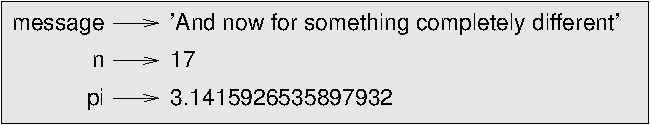
\includegraphics[scale=0.8]{figs/state2.pdf}}
\caption{แผนภาพสถานะ}
\label{fig.state2}
\end{figure}



\section{ชื่อตัวแปร} % (variable names)}
\index{variable}
\index{ตัวแปร}

โดยทั่วไปแล้ว นักเขียนโปรแกรมเลือกชื่อสำหรับตัวแปรที่มีความหมาย---พวกเขาทำการบันทึก
ว่าตัวแปรหนึ่ง ๆ เอาไว้ทำอะไรหรือเก็บค่าอะไร

ชื่อของตัวแปรสามารถยาวเท่าที่เราต้องการได้ ชื่อของตัวแปรสามารถมีทั้งตัวอักษรและตัวเลข
แต่ชื่อนั้นไม่สามารถขึ้นต้นด้วยตัวเลขได้  จริง ๆ แล้วเราสามารถขึ้นต้นชื่อตัวแปรด้วยอักษร
ตัวใหญ่ได้ แต่เรานิยมเริ่มต้นด้วยอักษรตัวเล็กซะมากกว่า

ในชื่อตัวแปรนั้นสามารถมีเครื่องหมายขีดล่าง (underscore), \verb|_|, ส่วนใหญ่แล้วเราจะ
ใช้ชื่อตัวแปรที่มีเครื่องหมายขีดล่างในชื่อที่ประกอบด้วยคำหลายคำ เช่น \verb|your_name| หรือ
 \verb|airspeed_of_unladen_swallow|
\index{underscore character}
\index{อักขระขีดล่าง}

ถ้าเราตั้งชื่อตัวแปรผิดกฎ เราจะได้ข้อผิดพลาดทางวากยสัมพันธ์ (syntax error) หรือข้อผิดพลาด
เชิงกฎเกณฑ์ของภาษา

\begin{verbatim}
>>> 76trombones = 'big parade'
SyntaxError: invalid syntax
>>> more@ = 1000000
SyntaxError: invalid syntax
>>> class = 'Advanced Theoretical Zymurgy'
SyntaxError: invalid syntax
\end{verbatim}
%
ชื่อตัวแปร {\tt 76trombones} นั้นผิดกฎเพราะว่ามันเริ่มด้วยตัวเลข
ส่วนชื่อตัวแปร {\tt more@} นั้นผิดกฎเพราะว่ามันมีอักขระต้องห้าม {\tt @}
แล้วสำหรับชื่อตัวแปร {\tt class} มันผิดอย่างไรกันนะ

ปรากฏว่า ชื่อตัวแปร {\tt class} นั้นเป็น {\bf คำสำคัญ (keywords)} ของภาษาไพธอน
ตัวแปลภาษาใช้คำสำคัญเหล่านี้ในการรู้จำโครงสร้างของโปรแกรม เราจึงไม่สามารถใช้คำสำคัญเหล่านี้
ในการตั้งชื่อตัวแปรได้
\index{keyword}
\index{คำสำคัญ}

ไพธอนเวอร์ชัน 3 มีคำสำคัญดังนี้:

\begin{verbatim}
False      class      finally    is         return
None       continue   for        lambda     try
True       def        from       nonlocal   while
and        del        global     not        with
as         elif       if         or         yield
assert     else       import     pass
break      except     in         raise
\end{verbatim}
%
เราไม่จำเป็นต้องจำคำสำคัญเหล่านี้ทั้งหมด ในโปรแกรมที่มีสภาพแวดล้อมสำหรับการพัฒนา 
(development environment) ส่วนใหญ่แล้วจะแสดงคำสำคัญเหล่านี้ โดยใช้สีที่แตกต่างจาก
โค้ดธรรมดา ถ้าเราพยายามจะใช้คำเหล่านี้ในโปรแกรม เราก็จะรู้ได้โดยสังเกตจากสีที่แตกต่างออกไป


\section{นิพจน์และคำสั่ง} % (expressions and statements)}

{\bf นิพจน์ (expression)} เป็นการรวมกันของค่า ตัวแปร และตัวดำเนินการต่าง ๆ
ค่า (value) เดี่ยว ๆ ก็ถือเป็นนิพจน์ เช่นเดียวกับ ตัวแปรเดี่ยว ๆ ด้วย
ดังนั้น สิ่งต่าง ๆ ต่อไปนี้ถือเป็นนิพจน์ที่ถูกต้องตามวากยสัมพันธ์
\index{expression}
\index{นิพจน์}

\begin{verbatim}
>>> 42
42
>>> n
17
>>> n + 25
42
\end{verbatim}
%
เมื่อเราพิมพ์นิพจน์ที่ข้อความพร้อมรับ (prompt) ตัวแปลภาษาจะทำการ {\bf ประเมินค่า (evaluates)}  
ซึ่งหมายความว่ามันจะหาค่าของนิพจน์นั้นออกมา ในตัวอย่างนี้ {\tt n} มีค่า 17
และ {\tt n + 25} มีค่าเท่ากับ 42
\index{evaluate}
\index{ประเมินค่า}

{\bf คำสั่ง (statement)} เป็นหน่วยของโค้ดที่ทำให้เกิดการทำงานต่าง ๆ เช่น สร้างตัวแปร หรือแสดงค่า
\index{statement}
\index{คำสั่ง}

\begin{verbatim}
>>> n = 17
>>> print(n)
\end{verbatim}
%
บรรทัดแรกเป็นคำสั่งที่ให้ค่ากับตัวแปร {\tt n}
บรรทัดที่สองเป็นคำสั่งพิมพ์ ที่ใช้แสดงค่าของตัวแปร {\tt n}

เมื่อเราพิมพ์คำสั่ง ตัวแปลภาษาจะ {\bf ดำเนินงาน (execute)} ตามคำสั่งนั้น ซึ่งหมายความว่า
มันจะทำตามที่คำสั่งนั้นบอกให้ทำ  โดยทั่วไปแล้ว คำสั่ง (statement) จะไม่มีค่าใด ๆ 
(ไม่ได้ให้ค่า หรือเก็บค่า)
\index{execute}
\index{ดำเนินงาน}


\section{โหมดสคริปต์} % (script mode)}

จนถึงตอนนี้ เราได้รันไพธอนใน {\bf โหมดโต้ตอบ (interactive mode)} ซึ่งหมายความว่า 
เราพิมพ์โค้ดเพื่อโต้ตอบโดยตรงกับตัวแปลภาษา โหมดโต้ตอบเป็นโหมดที่ดีสำหรับการเริ่มต้นเขียนโปรแกรม
แต่หากเราต้องการเขียนมากกว่าสองสามบรรทัด มันอาจจะดูงุ่มง่ามหน่อย
\index{interactive mode}
\index{โหมดโต้ตอบ}

อีกทางเลือกในการเขียนโปรแกรม คือ การเขียนและบันทึก (save) โค้ดลงในไฟล์ที่เรียกว่า 
{\bf สคริปต์ (script)} และให้ตัวแปลภาษาทำงานใน {\bf โหมดสคริปต์ (script mode)} 
เพื่อที่จะปฏิบัติตามสคริปต์นั้น เรานิยมตั้งชื่อไฟล์สคริปต์โดยใช้นามสกุล {\tt .py}  
\index{script}
\index{script mode}
\index{สคริปต์}
\index{โหมดสคริปต์}


ถ้าเกิดเรารู้ว่าจะสร้างและรันสคริปต์บนเครื่องคอมพิวเตอร์ของเราได้อย่างไร เราก็พร้อมที่จะไปต่อแล้ว
แต่หากยังไม่รู้ ผมแนะนำให้ใช้ระบบ PythonAnywhere อีกครั้ง ผมได้เขียนขั้นตอนการรัน
โหมดสคริปต์ในระบบที่ \url{http://tinyurl.com/thinkpython2e}.

เนื่องจากภาษาไพธอนสามารถทำงานได้ในทั้งสองโหมด เราสามารถทดสอบบางส่วนของโค้ดในโหมดโต้ตอบ
ก่อนที่จะเอาโค้ดไปวางในสคริปต์ได้ แต่มันก็มีความแตกต่างระหว่างสองโหมดนี้บางประการ
ที่ทำให้นักเขียนโปรแกรมสับสนได้เช่นกัน
\index{interactive mode}
\index{script mode}
\index{โหมดโต้ตอบ}
\index{โหมดสคริปต์}

ตัวอย่างเช่น ถ้าเราเอาไพธอนเป็นเครื่องคิดเลข เราจะพิมพ์ว่า

\begin{verbatim}
>>> miles = 26.2
>>> miles * 1.61
42.182
\end{verbatim}

บรรทัดแรกกำหนดค่าให้ตัวแปร {\tt miles} แต่มันไม่ได้มีผลที่แสดงให้เห็นได้
บรรทัดที่สองเป็นนิพจน์ ดังนั้น ตัวแปลภาษาจึงประเมินค่าและแสดงผลออกมาให้เราดู 
นั่นคือ ระยะทางของการวิ่งมาราธอน คือ ประมาณ 42 กิโลเมตร

แต่ถ้าเราพิมพ์โค้ดดังกล่าวในไฟล์สคริปต์และรันสคริปต์นั้น เราจะไม่ได้เห็นการแสดงค่าเลย
ในโหมดสคริปต์นั้น ตัวของนิพจน์เองจะไม่มีผลที่แสดงให้เห็นได้ ไพธอนจะมีการประเมินนิพจน์
นั้นอยู่ แต่มันจะไม่แสดงผลออกมาให้เห็น นอกจากเราจะบอกมันให้แสดง (โดยใช้คำสั่ง
แสดงผล): 

\begin{verbatim}
miles = 26.2
print(miles * 1.61)
\end{verbatim}

พฤติกรรมนี้อาจจะทำให้นักเขียนโปรแกรมงงได้ในตอนแรก ๆ

โดยปกติแล้ว ไฟล์สคริปต์จะมีลำดับของคำสั่ง ถ้ามีคำสั่งในสคริปต์มากกว่าหนึ่งคำสั่ง 
คำสั่งจะปฏิบัติและแสดงผลออกมาทีละคำสั่งตามลำดับ (จากบนลงล่าง)

ตัวอย่างเช่น ในสคริปต์ต่อไปนี้

\begin{verbatim}
print(1)
x = 2
print(x)
\end{verbatim}
%
ทำให้เกิดการแสดงผล คือ

\begin{verbatim}
1
2
\end{verbatim}
%
คำสั่งกำหนดค่า (assignment statement) ไม่ได้ทำให้เกิดการแสดงผลใด ๆ

เพื่อที่จะตรวจสอบความเข้าใจของเรา ให้พิมพ์คำสั่งต่อไปนี้ในตัวแปลภาษาไพธอน (โหมดโต้ตอบ) 
และลองดูว่ามันทำอะไรบ้าง:

\begin{verbatim}
5
x = 5
x + 1
\end{verbatim}

คราวนี้ ให้เอาคำสั่งข้างบนเดียวกันนี้ไปใส่ในไฟล์สคริปต์ แล้วลองรันดู
มันให้ผลอย่างไรบ้าง?

จากนั้น ให้แก้ไขแต่ละคำสั่งให้เป็นคำสั่งพิมพ์ (print) และลองรันดูอีกที



\section{ลำดับการดำเนินการ } %(orders of operations)}
\index{order of operations}
\index{PEMDAS}
\index{ลำดับการดำเนินการ}

เมื่อนิพจน์ประกอบด้วยตัวดำเนินการ (operator) มากกว่าหนึ่งตัว ลำดับของการประเมินผล
ค่านั้นจะขึ้นอยู่กับ {\bf ลำดับของตัวดำเนินการ (order of operations)} สำหรับ
ตัวดำเนินการทางคณิตศาสตร์ (mathematical operator) ไพธอนจะทำตามลำดับที่เป็น
ที่นิยมกันทั่วไป โดยให้เราจำตัวย่อ {\bf PEMDAS} เพื่อที่จะจำได้ง่ายขึ้น ดังนี้:

\begin{itemize}

\item {\bf P}arentheses หรือ วงเล็บ มีลำดับความสำคัญสูงที่สุด และสามารถใช้เพื่อ
บังคับให้นิพจน์ถูกประเมินค่าตามลำดับที่เราต้องการได้  เนื่องจากนิพจน์ในวงเล็บจะถูกประเมินค่า
ก่อน ดังนั้น {\tt 2 * (3-1)} จะมีค่าเท่ากับ 4 และ {\tt (1+1)**(5-2)} มีค่าเท่ากับ 8 
 เราสามารถใช้วงเล็บเขียนให้นิพจน์อ่านได้ง่ายขึ้นด้วย เช่น ในนิพจน์  {\tt (minute * 100) / 60} 
 ถึงแม้ว่าลำดับการประเมินค่าจะไม่เปลี่ยนเลยก็ตาม

\item {\bf E}xponentiation หรือการยกกำลัง มีลำดับความสำคัญมากที่สุดเป็นลำดับรองลงมา 
ดังนั้น {\tt 1 + 2**3} มีค่า 9 ไม่ใช่ 27 และ {\tt 2 * 3**2} มีค่าเป็น 18 ไม่ใช่ 36

\item {\bf M}ultiplication (การคูณ) และ {\bf D}ivision (การหาร) มีลำดับ
ความสำคัญมากกว่า {\bf A}ddition (การบวก) และ {\bf S}ubtraction การลบ ดังนั้น 
{\tt 2*3-1} มีค่าเป็น 5 ไม่ใช่ 4และ {\tt 6+4/2} มีค่าเป็น 8 ไม่ใช่ 5

\item ตัวดำเนินการที่มีลำดับความสำคัญเท่ากันจะถูกประเมินค่าจากซ้ายไปขวา (นอกจากการยกกำลัง)
 ดังนั้นในนิพจน์ {\tt degrees / 2 * pi} การหารจะถูกทำก่อน และผลของการหารจะถูกคูณด้วยค่า 
 {\tt pi} ถ้าเราต้องการจะหารด้วย $2 \pi$ เราสามารถใช้วงเล็บครอบ $2 \pi$ ไว้ หรือเขียนว่า 
 {\tt degrees / 2 / pi}

\end{itemize}

ผมเองไม่ค่อยจะได้ใส่ใจที่จะจำลำดับความสำคัญพวกนี้เท่าไหร่ แต่จะใช้วิธีว่า ถ้าเกิดผมมองนิพจน์ แล้ว
ประเมินค่าไม่ได้ทันที ก็จะใช้วิธีเขียนวงเล็บเพื่อจะทำให้นิพจน์นั้นชัดเจนขึ้นแทน


\section{การดำเนินการกับสายอักขระ } %(string operations)}
\index{string!operation}
\index{operator!string}
\index{การดำเนินการ!สายอักขระ}
\index{สายอักขระ!การดำเนินการ}

โดยทั่วไปแล้ว เราไม่สามารถดำเนินการทางคณิตศาสตร์กับสายอักขระได้ แม้ว่าสายอักขระจะดูเหมือนเป็น
ตัวเลขก็ตาม  ดังนั้น การทำดังต่อไปนี้จะผิดพลาดเชิงวากยสัมพันธ์:

\begin{verbatim}
'2'-'1'    'eggs'/'easy'    'third'*'a charm'
\end{verbatim}
%
แต่ก็มีข้อยกเว้นสำหรับ 2 อย่าง คือ เครื่องหมาย {\tt +} และ {\tt *}

ตัวดำเนินการ {\tt +} จะทำ {\bf การเชื่อมสายอักขระ (string concatenation)} 
ซึ่งหมายความว่ามันจะเชื่อมสายอักขระสองตัวเข้าด้วยกันทางด้านท้าย เช่น:
\index{concatenation}
\index{การเชื่อม}

\begin{verbatim}
>>> first = 'throat'
>>> second = 'warbler'
>>> first + second
throatwarbler
\end{verbatim}
%
ตัวดำเนินการ {\tt *} ยังสามารถทำงานกับสายอักขระได้ด้วย มันทำให้เกิดการทำซ้ำสายอักขระ เช่น 
\verb"'Spam'*3" ให้ผลว่า \verb"'SpamSpamSpam'" ถ้าตัวถูกดำเนินการตัวใดตัวหนึ่งเป็นสายอักขระ 
อีกตัวหนึ่งจะต้องเป็นจำนวนเต็มเสมอ (ไม่เช่นนั้นจะเกิดข้อผิดพลาดขึ้น) 

การใช้งาน {\tt +} และ {\tt *} ในลักษณะนี้ มันก็สอดคล้องกับการบวกและการคูณ
เปรียบเทียบกับการทำ {\tt 4*3} จะให้ค่าเท่ากับ {\tt 4+4+4} เราจึงคาดว่า \verb"'Spam'*3" 
ก็น่าจะให้ค่าเท่ากับ \verb"'Spam'+'Spam'+'Spam'" และมันก็เป็นเช่นนั้น  ในทางกลับกัน 
การต่อสายอักขระและการทำซ้ำสายอักขระ ก็มีความแตกต่างอย่างมากกับการบวกและคูณจำนวนเต็ม
เราลองคิดดูสิว่า มีคุณสมบัติอะไรบ้างที่การบวกจำนวนเต็มนั้นแตกต่างจากการต่อสายอักขระ
\index{commutativity}
\index{การสลับที่}


\section{คอมเมนต์ } %(Comments)}
\index{comment}
\index{คอมเมนต์}

เมื่อโปรแกรมเริ่มที่จะใหญ่ขึ้นและซับซ้อนมากขึ้น มันก็จะทำให้อ่านยากมากขึ้นด้วย  
พวกภาษาเชิงรูปแบบมักจะมีโค้ดหนาแน่นและมันยากที่จะดูส่วนต่าง ๆ ของโค้ด 
ว่าแต่ละส่วนมันทำอะไรบ้าง และทำไมจึงถูกเขียนขึ้นมาแบบนั้น

จากเหตุผลดังกล่าว มันเลยเป็นการดีที่จะเพิ่มคำอธิบายโค้ดสั้น ๆ เข้าไปในโปรแกรมด้วย 
เพื่ออธิบายให้เป็นภาษามนุษย์ ว่าโปรแกรมทำงานอะไรบ้าง คำอธิบายเหล่านี้เรียกว่า 
{\bf คอมเมนต์ (comments)} และส่วนของคอมเมนต์จะเริ่มด้วยสัญลักษณ์ \verb"#":

\begin{verbatim}
# compute the percentage of the hour that has elapsed
percentage = (minute * 100) / 60
\end{verbatim}
%
ในกรณีนี้ คอมเมนต์อยู่ในบรรทัดเดี่ยว ๆ ของมันเอง  นอกจากนี้เรายังสามารถใส่คอมเมนต์
เข้าไปในท้ายบรรทัดของคำสั่งต่าง ๆ ได้ด้วย:

\begin{verbatim}
percentage = (minute * 100) / 60     # percentage of an hour
\end{verbatim}
%
ทุกอย่างตั้งแต่สัญลักษณ์ {\tt \#} ไปจนถึงจบบรรทัดนั้นจะถูกเมินโดยโปรแกรม---
มันจะไม่มีผลกับการทำงานของโปรแกรมเลย

คอมเมนต์จะมีประโยชน์มากที่สุดเมื่อใช้อธิบายลักษณะเฉพาะของโปรแกรมที่เข้าใจได้ยาก 
หรือไม่ชัดเจน  มันเหมาะสมที่เราจะสมมติว่าผู้ที่อ่านโค้ดนั้นเข้าใจว่าโค้ด {\em ทำอะไร}  
ดังนั้น จะมีประโยชน์มากกว่าที่จะอธิบายว่าโค้ดนั้นมีไว้ {\em ทำไม}

คอมเมนต์ข้างล่างนี้ซ้ำซ้อนกับโค้ดและไม่มีประโยชน์:

\begin{verbatim}
v = 5     # assign 5 to v
\end{verbatim}
%
ส่วนคอมเมนต์ต่อไปนี้ มีข้อมูลที่เป็นประโยชน์ที่ไม่ได้อยู่ในโค้ด:

\begin{verbatim}
v = 5     # velocity in meters/second. 
\end{verbatim}
%
การตั้งชื่อตัวแปรให้ดีมีความหมายจะช่วยลดความจำเป็นในการมีคอมเมนต์ แต่ถ้าชื่อตัวแปร
ยาวเกินไปก็อาจจะทำให้นิพจน์ที่ซับซ้อนนั้นอ่านยาก เราต้องลองชั่งน้ำหนักดู


\section{การดีบัก}
\index{debugging}
\index{bug}
\index{การดีบัก}
\index{บัก}

ข้อผิดพลาดในโปรแกรมสามารถเกิดได้ 3 แบบ: ข้อผิดพลาดเชิงวากยสัมพันธ์ (syntax error), 
ข้อผิดพลาดเวลาดำเนินการ (runtime error) และ ข้อผิดพลาดเชิงความหมาย (semantic error) 
เวลาเกิดข้อผิดพลาดมันจะเป็นประโยชน์ ถ้าเราสามารถแยกแยะได้ว่า เป็นความผิดพลาดประเภทใด
เพื่อที่จะหาสาเหตุได้เร็วขึ้น

\begin{description}

\item[ข้อผิดพลาดเชิงวากยสัมพันธ์ (Syntax error):] ``syntax'' หมายความถึงโครงสร้างของ
โปรแกรม และกฎเกณฑ์ต่าง ๆ ที่เกี่ยวกับโครงสร้างนั้น เช่น วงเล็บจะต้องมีคู่เปิดปิดให้ครบ ดังนั้น 
{\tt (1 + 2)}  จะถูกกฎ แต่ {\tt 8)} จะเป็นข้อผิดพลาดเชิงวากยสัมพันธ์ 
 \index{syntax error} \index{error!syntax}
 \index{error message} \index{syntax} 
 \index{ข้อผิดพลาดเชิงวากยสัมพันธ์} \index{ข้อผิดพลาด!วากยสัมพันธ์}
 \index{ข้อความแจ้งข้อผิดพลาด} \index{วากยสัมพันธ์} 

 หากเกิดข้อผิดพลาดเชิงวากยสัมพันธ์สักแห่งในโปรแกรม ไพธอนจะแสดงข้อความระบุข้อผิดพลาด (error 
 message) และออกจากโปรแกรมไป และเราก็จะไม่สามารถรันโปรแกรมนั้นได้ ในช่วงเวลาที่เราเริ่มฝึกเขียน 
 2-3 สัปดาห์แรก เราอาจจะต้องเวลามากในการหาสาเหตุของข้อผิดพลาดเชิงวากยสัมพันธ์ แต่เมื่อเรามี
 ประสบการณ์ในการเขียนโปรแกรมมากขึ้นแล้ว เราอาจจะมีข้อผิดพลาดเหล่านี้น้อยลงและหาต้นตอได้เร็วขึ้น


\item[ข้อผิดพลาดตอนดำเนินการ (Runtime error):] ข้อผิดพลาดแบบที่สอง คือ ข้อผิดพลาดตอน
ดำเนินการ (เวลารันโปรแกรม)  เราเรียกแบบนั้น เพราะว่าข้อผิดพลาดแบบนี้จะไม่เกิดขึ้นจนกว่าโปรแกรม
จะเริ่มรัน  เรายังเรียกข้อผิดพลาดแบบนี้ได้ว่า {\bf ข้อยกเว้น (exceptions)} เพราะโดยปกติแล้วมันจะ
หมายความว่า มีข้อยกเว้นในการทำงานเกิดขึ้น (และแย่ด้วย)
 \index{runtime error} \index{error!runtime}
 \index{exception} \index{safe language} \index{language!safe}
 \index{ข้อผิดพลาดตอนดำเนินการ} \index{ข้อผิดพลาด!ตอนดำเนินการ}
 \index{ข้อยกเว้น} \index{ภาษาที่ปลอดภัย} \index{ภาษา!ปลอดภัย}

 ข้อผิดพลาดตอนดำเนินการนั้น เกิดได้ยากในโปรแกรมพื้นฐานที่เราจะได้เห็นใน 2-3 บทแรกนี้ 
 ดังนั้น อีกสักพักเลยเราถึงจะเจอข้อผิดพลาดแบบนี้


\item[ข้อผิดพลาดเชิงความหมาย (Semantic error):] ข้อผิดพลาดอย่างที่สาม คือ ``semantic'' 
ซึ่งเกี่ยวกับความหมายของคำสั่ง ถ้าหากโปรแกรมของเราเกิดข้อผิดพลาดเชิงความหมาย โปรแกรมจะยังคงทำงาน
ได้อยู่โดยไม่มีข้อความระบุข้อผิดพลาดใด ๆ  แต่มันจะทำให้โปรแกรมนั้นทำงานไม่ถูกต้องตามที่เราต้องการ 
มันจะทำอย่างอื่นแทน นั่นคือ มันจะทำอะไรที่เราบอกให้มันทำ 

(หมายเหตุผู้แปล: อาจจะไม่ใช่สิ่งที่เราต้องการทำจริง ๆ คือ เราบอกมันผิดจากที่เราต้องการนั่นเอง)
 \index{semantic error}
 \index{error!semantic}  \index{error message}
 \index{ข้อผิดพลาดเชิงความหมาย}
 \index{ข้อผิดพลาด!ความหมาย}  \index{ข้อความแจ้งข้อผิดพลาด}

การระบุข้อผิดพลาดเชิงความหมายอาจจะลำบากหน่อย เพราะเราจะต้องกลับไปไล่ดูผลการทำงานของโปรแกรม
และพยายามที่จะหาว่าโปรแกรมมันทำอะไรกันแน่ (และทำพลาดตรงไหน)

\end{description}


\section{อภิธานศัพท์}

\begin{description}

\item[ตัวแปร (variable):]  ชื่อที่อ้างถึงค่าค่าหนึ่ง (ในหน่วยความจำ)
\index{variable}
\index{ตัวแปร}

\item[การกำหนดค่า (assignment):]  คำสั่งที่กำหนดค่าให้ตัวแปร
\index{assignment}
\index{การกำหนดค่า}

\item[แผนภาพสถานะ (state diagram):]  รูปที่แสดงตัวแปรและค่าที่มันอ้างถึง
\index{state diagram}
\index{แผนภาพสถานะ}

\item[คำสำคัญ (keyword):]  คำที่สงวนไว้สำหรับแยกวิเคราะห์ส่วนต่าง ๆ ของโปรแกรม 
เราไม่สามารถใช้คำสำคัญ เช่น {\tt if}, {\tt  def}, และ {\tt while} เพื่อเป็นชื่อของตัวแปรได้
\index{keyword}
\index{คำสำคัญ}

\item[ตัวถูกดำเนินการ (operand):] ค่าที่ตัวดำเนินการ (operator) ใช้ทำงาน
\index{operand}
\index{ตัวถูกดำเนินการ}

\item[นิพจน์ (expression):]  การประกอบกันของตัวแปร ตัวดำเนินการ และค่าค่าง ๆ 
ที่ทำให้เกิดผลอย่างใดอย่างหนึ่ง
\index{expression}
\index{นิพจน์}

\item[ประเมินค่า (evaluate):]  การทำให้นิพจน์นั้นง่ายขึ้น ด้วยการดำเนินการต่าง ๆ 
เพื่อให้เหลือแค่ค่าเดียว

\item[คำสั่ง (statement):]  ส่วนของโค้ดที่เป็นการสั่งงาน หรือ การกระทำ จนถึงตอนนี้ 
คำสั่งที่เราเจอมีแค่คำสั่งกำหนดค่าและคำสั่งพิมพ์
\index{statement}
\index{คำสั่ง}

\item[ดำเนินงาน (execute):]  รันคำสั่งและทำตามคำสั่ง
\index{execute}
\index{ดำเนินงาน}

\item[โหมดโต้ตอบ (interactive mode):] วิธีการใช้ตัวแปลภาษาไพธอนโดยการพิมพ์โค้ดที่ prompt เลย
\index{interactive mode}
\index{โหมดโต้ตอบ}

\item[โหมดสคริปต์ (script mode):] วิธีการใช้ตัวแปลภาษาไพธอนโดยการให้อ่านโค้ดจากสคริปต์
และรันสคริปต์
\index{script mode}
\index{โหมดสคริปต์}

\item[สคริปต์ (script):] โปรแกรมที่ถูกเก็บในไฟล์
\index{script}
\index{สคริปต์}

\item[ลำดับการดำเนินการ (order of operations):] กฎที่กำหนดลำดับการประเมินค่าในนิพจน์ที่มี
ตัวดำเนินการและตัวถูกดำเนินการหลายตัว  
\index{order of operations} 
\index{ลำดับการดำเนินการ}

\item[เชื่อม (concatenate):]  เชื่อมตัวถูกดำเนินการสองตัวเข้าด้วยกันทางด้านท้าย
\index{concatenation} 
\index{การเชื่อม}

\item[คอมเมนต์ (comment):]  ข้อมูลในโปรแกรมที่เขียนขึ้นสำหรับนักเขียนโปรแกรมคนอื่น (หรือ
ใครก็ตามที่อ่านโค้ด) ให้เข้าใจโค้ด และมันไม่มีผลต่อการดำเนินการหรือการทำงานของโปรแกรม 
\index{comment} 
\index{คอมเมนต์}

\item[ข้อผิดพลาดเชิงวากยสัมพันธ์ (syntax error):]  ข้อผิดพลาดในโปรแกรมที่ทำให้โปรแกรมแยกแยะ
โครงสร้างไม่ได้ (และทำให้แปลความหมายของโปรแกรมไม่ได้) 
\index{syntax error} 
\index{ข้อผิดพลาดเชิงวากยสัมพันธ์}

\item[ข้อยกเว้น (exception):]  ข้อผิดพลาดที่ถูกพบตอนที่โปรแกรมกำลังทำงานอยู่
\index{exception} 
\index{ข้อยกเว้น}

\item[อรรถศาสตร์ (semantics):]  ความหมายของโปรแกรม
\index{semantics} 
\index{อรรถศาสตร์}

\item[ข้อผิดพลาดเชิงความหมาย (semantic error):]   ข้อผิดพลาดในโปรแกรมที่ทำให้โปรแกรม
ทำงานอย่างอื่น นอกเหนือจากที่นักเขียนโปรแกรมตั้งใจให้เป็น 
\index{semantic error} 
\index{ข้อผิดพลาดเชิงความหมาย}

\end{description}


\section{แบบฝึกหัด}

\begin{exercise}

ขอย้ำคำแนะนำจากบทที่แล้ว เมื่อไหร่ก็ตามที่เราได้เรียนรู้ลักษณะเฉพาะใหม่ ๆ ของภาษา 
เราควรที่จะต้องทดลองในโหมดโต้ตอบ และลองทำให้เกิดข้อผิดพลาดต่าง ๆ 
เพื่อที่จะดูว่าจะเกิดอะไรขึ้นได้บ้าง

\begin{itemize}

\item เราเห็นแล้วว่า {\tt n = 42} มันถูกต้องตามวากยสัมพันธ์  แล้วถ้าเป็น {\tt 42 = n} ล่ะ?

\item แล้วถ้าเป็น {\tt x = y = 1} ล่ะ?

\item ในบางภาษา ทุกคำสั่งจะจบด้วยเครื่องหมายอัฒภาค (จุดครึ่ง หรือ เซมิโคลอน), {\tt ;} 
มันจะเกิดอะไรขึ้นถ้าเราใส่เครื่องหมาย {\tt ;} ในตอนท้ายของคำสั่งไพธอน?

\item แล้วถ้าใส่จุดในท้ายคำสั่งไพธอนล่ะ?

\item ในสัญกรณ์ทางคณิตศาสตร์ (math notation) เราสามารถคูณ $x$ กับ $y$ แบบนี้ได้: $x y$
จะเกิดอะไรขึ้นถ้าเราลองทำแบบนี้บ้างในไพธอน?

\end{itemize}

\end{exercise}


\begin{exercise}

ให้ฝึกการใช้ตัวแปลภาษาไพธอนให้เป็นเครื่องคิดเลข: 
\index{calculator}
\index{เครื่องคิดเลข}

\begin{enumerate}

\item ปริมาตรของทรงกลมที่มีรัศมี $r$ คือ $\frac{4}{3} \pi r^3$
แล้วปริมาตรของทรงกลมที่มีรัศมีเท่ากับ 5 เป็นเท่าไหร่

\item สมมติว่า ราคาหน้าปกหนังสือ คือ \$24.95 แต่ร้านหนังสือลดราคาให้ 40\% ค่าส่งหนังสือ คือ 
\$3 สำหรับเล่มแรก และ 75 เซ็นต์ (\$0.75) สำหรับแต่ละเล่มที่เพิ่มขึ้นมา ราคาของการซื้อหนังสือ
จำนวน 60 เล่มจะเป็นเท่าไหร่

\item ถ้าเราออกจากบ้านในเวลา 6:52 และวิ่ง 1 ไมล์แบบเบา ๆ  (8:15 นาทีต่อไมล์) 
จากนั้นวิ่งทำเวลาเป็นจำนวน 3 ไมล์ (7:12 นาทีต่อไมล์) และจบด้วยวิ่งเบา ๆ อีก 1 ไมล์ 
แล้วเราจะได้กลับบ้านไปกินข้าวเช้าในเวลาใด
\index{running pace}
\index{เพซการวิ่ง}

\end{enumerate}
\end{exercise}



\chapter{ฟังก์ชัน } %(functions)}
\label{funcchap}


ในบริบทของการเขียนโปรแกรม {\bf ฟังก์ชัน (function)} เป็นลำดับของคำสั่งต่าง ๆ ที่ทำงาน
ต่อเนื่องกันที่ถูกกำหนดชื่อให้  เมื่อเรานิยามฟังก์ชัน เราต้องระบุชื่อและลำดับของคำสั่งต่าง ๆ 
หลังจากนั้น เราสามารถ ``เรียก'' ฟังก์ชันโดยใช้ชื่อที่ระบุไว้ได้
\index{function}
\index{ฟังก์ชัน}

\section{การเรียกฟังก์ชัน} % (Function calls)}
\label{functionchap}
\index{function call}
\index{การเรียกฟังก์ชัน}

เราได้เห็นตัวอย่างหนึ่งของการเรียกฟังก์ชันไปแล้ว:

\begin{verbatim}
>>> type(42)
<class 'int'>
\end{verbatim}
%
ชื่อของฟังก์ชันนี้คือ {\tt type} นิพจน์ในวงเล็บ เรียกว่า {\bf อาร์กิวเมนต์ (argument)} ของฟังก์ชัน
ผลลัพธ์ของฟังก์ชันนี้ คือ ชนิดของฟังก์ชัน (ในกรณีนี้ คือ ชนิดจำนวนเต็ม (int))  
\index{parentheses!argument in}
\index{วงเล็บ!อาร์กิวเมนต์ อยู่ใน}

โดยปกติแล้วเราพูดได้ว่า ฟังก์ชันจะ ``รับ'' อาร์กิวเมนต์ และ ``ส่งคืน'' ค่าผลลัพธ์ของฟังก์ชัน
ผลลัพธ์นี้ยังสามารถเรียกว่า ``ค่าคืนกลับ'' ได้อีกด้วย 
\index{argument}
\index{return value}
\index{อาร์กิวเมนต์}
\index{ค่าคืนกลับ}

ไพธอนได้เตรียมฟังก์ชันที่แปลงค่าจากชนิดหนึ่งไปยังอีกชนิดหนึ่งไว้ให้ ฟังก์ชัน {\tt int} รับค่าอะไรก็ได้
และแปลงค่าที่รับมานั้นไปเป็นจำนวนเต็มถ้ามันสามารถทำได้ ถ้าทำไม่ได้มันก็จะบ่นใส่เรา: 
\index{conversion!type}
\index{type conversion}
\index{int function}
\index{function!int}
\index{การแปลง!ชนิด}
\index{การแปลงชนิด}
\index{ฟังก์ชัน int}
\index{ฟังก์ชัน!int}

\begin{verbatim}
>>> int('32')
32
>>> int('Hello')
ValueError: invalid literal for int(): Hello
\end{verbatim}
%
ฟังก์ชัน {\tt int} สามารถแปลงเลขจำนวนจุดลอย (floating-point) ไปเป็นจำนวนเต็มได้
แต่มันไม่ได้ใช้การปัดเศษ (ขึ้นหรือลง) มันจะตัดจุดทศนิยมออกไปเลย: 

\begin{verbatim}
>>> int(3.99999)
3
>>> int(-2.3)
-2
\end{verbatim}
%
ฟังก์ชัน {\tt float} แปลงจำนวนเต็มและสายอักขระไปเป็นจำนวนจุดลอย:
\index{float function}
\index{function!float}
\index{ฟังก์ชัน float}
\index{ฟังก์ชัน!float}

\begin{verbatim}
>>> float(32)
32.0
>>> float('3.14159')
3.14159
\end{verbatim}
%
อย่างสุดท้าย ฟังก์ชัน {\tt str} แปลงอาร์กิวเมนต์ของมันไปเป็นสายอักขระ:
\index{str function}
\index{function!str}
\index{ฟังก์ชัน str}
\index{ฟังก์ชัน!str}

\begin{verbatim}
>>> str(32)
'32'
>>> str(3.14159)
'3.14159'
\end{verbatim}
%


\section{ฟังก์ชันทางคณิตศาสตร์} % (Math functions)}
\index{math function}
\index{function, math}
\index{ฟังก์ชันทางคณิตศาสตร์}
\index{ฟังก์ชัน, คณิตศาสตร์}

ไพธอนมีมอดูลสำหรับฟังก์ชันทางคณิตศาสตร์ที่เราคุ้นเคยกัน  {\bf มอดูล (module)} 
เป็นไฟล์ที่บรรจุกลุ่มของฟังก์ชันที่เกี่ยวข้องกันไว้ด้วยกัน
\index{module}
\index{module object}
\index{มอดูล}
\index{วัตถุมอดูล}

ก่อนที่เราจะใช้ฟังก์ชันจากมอดูลใด ๆ เราจะต้องนำเข้า (import) มอดูลนั้นก่อน ด้วย 
{\bf คำสั่งนำเข้า (import statement)}


\begin{verbatim}
>>> import math
\end{verbatim}
%
คำสั่งนี้สร้าง {\bf วัตถุมอดูล (module object)} ที่ชื่อว่า math 
ถ้าเราสั่งให้แสดงวัตถุมอดูลอันนี้ เราจะได้ข้อมูลเกี่ยวกับตัววัตถุออกมา:

\begin{verbatim}
>>> math
<module 'math' (built-in)>
\end{verbatim}
%
วัตถุมอดูลบรรจุฟังก์ชันต่าง ๆ และตัวแปรต่าง ๆ ที่ถูกนิยามขึ้นในมอดูล ในการเข้าถึงฟังก์ชันหนึ่ง ๆ
ที่อยู่ในมอดูลนี้ เราจะต้องระบุชื่อของมอดูลและชื่อของฟังก์ชันที่เราต้องการ โดยการคั่นด้วยจุด 
รูปแบบดังกล่าว เรียกว่า {\bf สัญกรณ์จุด (dot notation)}
\index{dot notation}
\index{สัญกรณ์จุด}

\begin{verbatim}
>>> ratio = signal_power / noise_power
>>> decibels = 10 * math.log10(ratio)

>>> radians = 0.7
>>> height = math.sin(radians)
\end{verbatim}
%
ตัวอย่างแรกใช้ฟังก์ชัน \verb"math.log10" ในการคำนวณอัตราส่วนของสัญญานต่อการรบกวน 
ในหน่วยเดซิเบล (สมมติว่า \verb|signal_power| และ \verb|noise_power| ได้ถูกนิยามไปแล้ว) 
มอดูล math ได้จัดเตรียมฟังก์ชัน {\tt log} ซึ่งจะคำนวณค่า log ฐาน {\tt e} ไว้ให้แล้ว
\index{log function}
\index{function!log}
\index{sine function}
\index{radian}
\index{trigonometric function}
\index{function, trigonometric}
\index{ฟังก์ชัน log}
\index{ฟังก์ชัน!log}
\index{ฟังก์ชัน sin}
\index{เรเดียน}
\index{ฟังก์ชันตรีโกณมิติ}
\index{ฟังก์ชัน, ตรีโกณมิติ}

ตัวอย่างที่สองเป็นการหาค่า sin ของตัวแปร {\tt radians} ซึ่งชื่อของตัวแปรนี้ใบ้ให้เราทราบว่า 
ฟังก์ชัน {\tt sin} และฟังก์ชันอื่นในตรีโกณมิติ ({\tt cos}, {\tt tan}, 
และอื่น ๆ) นั้น รับอาร์กิวเมนต์ในหน่วยเรเดียน (radian)  การแปลงจากหน่วยองศา (degree) 
มาเป็นหน่วยเรเดียนนั้น เราจะหารด้วย 180 และคูณด้วย $\pi$:

\begin{verbatim}
>>> degrees = 45
>>> radians = degrees / 180.0 * math.pi
>>> math.sin(radians)
0.707106781187
\end{verbatim}
%
นิพจน์ {\tt math.pi} นำตัวแปร {\tt pi} มาจากมอดูล math ค่าของมันเป็นค่าจุดลอย
ที่ประมาณค่าของ $\pi$ มาอีกที โดยมีจุดทศนิยมประมาณ 15 ตำแหน่ง
\index{pi}
\index{พาย}

ถ้าเรารู้จักตรีโกณมิติ เราจะสามารถตรวจสอบผลการทำงานก่อนหน้านี้ โดยเปรียบเทียบกับค่ารากที่สองของ 2 
แล้วหารด้วย 2:
\index{sqrt function}
\index{function!sqrt}
\index{ฟังก์ชัน sqrt}
\index{ฟังก์ชัน!sqrt}

\begin{verbatim}
>>> math.sqrt(2) / 2.0
0.707106781187
\end{verbatim}
%


\section{การประกอบ} % (Composition)}
\index{composition}
\index{การประกอบ}

ถึงตอนนี้ เราได้ดูส่วนประกอบต่าง ๆ ของโปรแกรม---ตัวแปร นิพจน์ คำสั่ง---แบบแยกกัน 
โดยที่ไม่ได้พูดถึงว่า เราจะประกอบมันเข้าด้วยกันได้อย่างไร

ลักษณะเฉพาะที่ทรงพลังที่สุดอย่างหนึ่งของภาษาการเขียนโปรแกรม นั่นคือ การที่พวกมันสามารถ
เอาบล็อกก่อสร้างเล็ก ๆ มา {\bf ประกอบ} เข้าด้วยกัน เช่น การที่อาร์กิวเมนต์ของฟังก์ชัน สามารถเป็น
นิพจน์แบบไหนก็ได้ รวมถึงตัวดำเนินการทางคณิตศาสตร์ด้วย:

\begin{verbatim}
x = math.sin(degrees / 360.0 * 2 * math.pi)
\end{verbatim}
%
และแม้แต่การเรียกฟังก์ชัน:

\begin{verbatim}
x = math.exp(math.log(x+1))
\end{verbatim}
%
ในเกือบทุกที่ เราสามารถใส่ค่านิพจน์ใด ๆ ได้ ยกเว้นหนึ่งที่: ทางซ้ายของการกำหนดค่า
จะต้องเป็นชื่อตัวแปร การวางนิพจน์แบบอื่นทางซ้ายนั้น จะเป็นข้อผิดพลาดเชิงวากยสัมพันธ์ (syntax error) 
(เราจะได้เห็นข้อยกเว้นของกฎข้อนี้ในภายหลัง)

\begin{verbatim}
>>> minutes = hours * 60                 # right
>>> hours * 60 = minutes                 # wrong!
SyntaxError: can't assign to operator
\end{verbatim}
%
\index{SyntaxError}
\index{exception!SyntaxError}
\index{ข้อผิดพลาดเชิงวากยสัมพันธ์}
\index{ข้อยกเว้น!ข้อผิดพลาดเชิงวากยสัมพันธ์}


\section{การเพิ่มฟังก์ชันใหม่} % (Adding new functions)}

ถึงตอนนี้ เราได้ใช้แค่ฟังก์ชันที่มากับไพธอน แต่มันเป็นไปได้ที่เราจะเพิ่มฟังก์ชันต่าง ๆ เข้าไปใหม่
{\bf นิยามของฟังก์ชัน (function definition)} ระบุชื่อของฟังก์ชัน และกลุ่มของคำสั่ง
ที่ต่อเนื่องกันในฟังก์ชัน ซึ่งคำสั่งเหล่านี้จะทำงานเมื่อฟังก์ชันถูกเรียกใช้
\index{function}
\index{function definition}
\index{definition!function}
\index{ฟังก์ชัน}
\index{นิยามของฟังก์ชัน}
\index{นิยาม!ฟังก์ชัน}

นี่คือตัวอย่าง:

\begin{verbatim}
def print_lyrics():
    print("I'm a lumberjack, and I'm okay.")
    print("I sleep all night and I work all day.")
\end{verbatim}
%
{\tt def} เป็นคำสำคัญที่ระบุว่า นี่คือ นิยามของฟังก์ชัน  ชื่อของฟังก์ชัน คือ \verb|print_lyrics|
กฎการตั้งชื่อฟังก์ชันนั้นเหมือนกับกฎการตั้งชื่อตัวแปร: ตัวอักษร ตัวเลข และขีดล่างนั้นใช้ได้ 
แต่อักขระตัวแรกต้องไม่เป็นตัวเลข เราไม่สามารถใช้คำสำคัญเป็นชื่อของฟังก์ชัน และเราต้องหลีกเลี่ยง
การใช้ชื่อตัวแปรและชื่อฟังก์ชันที่เหมือนกัน
\index{def keyword}
\index{keyword!def}
\index{argument}
\index{คำสำคัญ def}
\index{คำสำคัญ!def}
\index{อาร์กิวเมนต์}

วงเล็บว่างหลังชื่อฟังก์ชัน ระบุว่าฟังก์ชันนี้ไม่รับอาร์กิวเมนต์ใด ๆ เข้ามาในฟังก์ชัน
\index{parentheses!empty}
\index{header}
\index{body}
\index{indentation}
\index{colon}
\index{วงเล็บ!ว่าง}
\index{ส่วนหัว}
\index{ส่วนตัว}
\index{ย่อหน้า}
\index{ทวิภาค} \index{โคลอน}


บรรทัดแรกของนิยามฟังก์ชันเรียกว่า {\bf ส่วนหัว (header)}; ที่เหลือเรียกว่า {\bf ส่วนตัว (body)}
ส่วนหัวจะต้องลงท้ายด้วยเครื่องหมายทวิภาค (จุดคู่ หรือ โคลอน) (:) และส่วนตัวของฟังก์ชันจะต้อง
ย่อหน้าเข้าไป การย่อหน้าเข้าไปนิยมใช้ช่องว่าง (space) 4 ตำแหน่ง ตัวของฟังก์ชันสามารถบรรจุคำสั่ง
กี่คำสั่งก็ได้

(หมายเหตุผู้แปล: การย่อหน้าสามารถใช้ tab ได้ แต่ต้องเลือกการย่อหน้าให้เป็นรูปแบบเดียวกันทั้งไฟล์)

สายอักขระที่อยู่ในคำสั่งพิมพ์ถูกใส่อยู่ในเครื่องหมายอัญประกาศ  อัญประกาศเดี่ยว (single quotes) 
และอัญประกาศ (double quotes) ทำงานเหมือนกัน คนส่วนใหญ่ใช้อัญประกาศเดี่ยว 
ยกเว้นในกรณีอย่างเช่น การมีเครื่องหมายอัญประกาศเดี่ยวตัวเดียว (apostrophe) ในสายอักขระ

อัญประกาศทุกแบบจะต้องเป็นเครื่องหมายที่เป็น ``เส้นตรง ๆ`` ซึ่งโดยปกติแล้วจะอยู่ถัดจากปุ่ม Enter 
บนคีย์บอร์ด ส่วนเครื่องหมายอัญประกาศ ``แบบโค้ง'' เช่นในประโยคนี้ จะผิดกฎของไพธอน

ถ้าเราพิมพ์นิยามของฟังก์ชันในโหมดโต้ตอบ ตัวแปลภาษาไพธอนจะขึ้นจุดหลาย ๆ จุด ({\tt ...}) มาให้
เพื่อที่เราจะได้รู้ว่านิยามฟังก์ชันนั้นยังไม่สมบูรณ์ดี 
\index{ellipses}
\index{การละไว้}

\begin{verbatim}
>>> def print_lyrics():
...     print("I'm a lumberjack, and I'm okay.")
...     print("I sleep all night and I work all day.")
...
\end{verbatim}
%
ถ้าต้องการจบฟังก์ชัน ให้เรา enter บรรทัดเปล่า ๆ เข้าไปหนึ่งบรรทัด

การนิยามฟังก์ชันจะสร้าง {\bf วัตถุฟังก์ชัน (function object)} ที่มีชนิดเป็น \verb"function":
\index{function type}
\index{type!function}
\index{ชนิดของฟังก์ชัน}
\index{ชนิด!ฟังก์ชัน}

\begin{verbatim}
>>> print(print_lyrics)
<function print_lyrics at 0xb7e99e9c>
>>> type(print_lyrics)
<class 'function'>
\end{verbatim}
%
กฎวากยสัมพันธ์ในการเรียกฟังก์ชันใหม่นั้นเหมือนกับการเรียกฟังก์ชันพร้อมใช้ (built-in function):

\begin{verbatim}
>>> print_lyrics()
I'm a lumberjack, and I'm okay.
I sleep all night and I work all day.
\end{verbatim}
%
เมื่อเราได้นิยามฟังก์ชันแล้ว เราสามารถใช้มันในฟังก์ชันอื่นได้ด้วย เช่น ถ้าเราต้องการจะพิมพ์เนื้อเพลงบทที่แล้วอีกรอบ
เราสามารถเขียนฟังก์ชันที่ชื่อว่า \verb|repeat_lyrics|:

\begin{verbatim}
def repeat_lyrics():
    print_lyrics()
    print_lyrics()
\end{verbatim}
%
จากนั้น ให้เรียก \verb|repeat_lyrics|:

\begin{verbatim}
>>> repeat_lyrics()
I'm a lumberjack, and I'm okay.
I sleep all night and I work all day.
I'm a lumberjack, and I'm okay.
I sleep all night and I work all day.
\end{verbatim}
%
แต่จริง ๆ แล้วเนื้อเพลงมันไม่ได้เป็นแบบนั้นหรอกนะ


\section{นิยามและการใช้งาน} % (Definitions and uses)}
\index{function definition}
\index{นิยามของฟังก์ชัน}

เมื่อทำการรวบรวมโค้ดชิ้นต่าง ๆ จากเนื้อหาในส่วนที่ผ่านมา โปรแกรมที่สมบูรณ์ก็จะหน้าตาเป็นแบบนี้:

\begin{verbatim}
def print_lyrics():
    print("I'm a lumberjack, and I'm okay.")
    print("I sleep all night and I work all day.")

def repeat_lyrics():
    print_lyrics()
    print_lyrics()

repeat_lyrics()
\end{verbatim}
%
โปรแกรมนี้ประกอบด้วยนิยามฟังก์ชัน 2 ตัว: \verb|print_lyrics| และ \verb|repeat_lyrics|
นิยามฟังก์ชันทำงานเหมือนคำสั่งต่าง ๆ ทั่วไป แต่จะส่งผลให้เกิดการสร้างวัตถุฟังก์ชัน  คำสั่งต่าง ๆ ที่อยู่ใน
ฟังก์ชันจะไม่ทำงานจนกว่าฟังก์ชันนั้นจะถูกเรียก และตัวนิยามของฟังก์ชันเองจะไม่ทำให้เกิดผลลัพธ์ใด ๆ 

(หมายเหตุผู้แปล: นั่นคือ จะต้องมีการเรียกฟังก์ชันก่อน ถึงจะมีการทำงานใด ๆ นั่นเอง)
\index{use before def}
\index{การใช้ก่อนการนิยาม}

เราอาจจะพอคาดได้ว่า เราจะต้องสร้างฟังก์ชันก่อนที่เราจะเรียกมันใช้งาน อีกนัยหนึ่งคือ นิยามของฟังก์ชัน
จะต้องถูกรันก่อนที่ฟังก์ชันนั้นจะถูกเรียกใช้งาน

เพื่อเป็นการฝึก ให้ลองย้ายบรรทัดสุดท้ายของโปรแกรมไปไว้ข้างบนสุด ซึ่งทำให้การเรียกฟังก์ชันนั้นเกิดก่อน
การนิยามฟังก์ชัน ให้รันโปรแกรมและดูว่าไพธอนจะให้ข้อความแจ้งข้อผิดพลาดอะไรออกมา

คราวนี้ ให้ย้ายการเรียกฟังก์ชันกลับมาข้างล่างสุดเหมือนเดิม และย้ายนิยามของ \verb|print_lyrics|
ให้ไปอยู่หลังนิยามของ \verb|repeat_lyrics| จะเกิดอะไรขึ้นเมื่อเรารันโปรแกรมนี้?


\section{กระแสการดำเนินการ} % (Flow of execution)}
\index{flow of execution}
\index{กระแสการดำเนินการ}

% To ensure that a function is defined before its first use,
% you have to know the order statements run in, which is
% called the {\bf flow of execution}.
เพื่อที่ให้แน่ใจว่าฟังก์ชันนั้นถูกนิยามก่อนการใช้งานครั้งแรก เราต้องรู้ลำดับการทำงานของคำสั่งก่อน
ซึ่งเรียกว่า {\bf กระแสการดำเนินการ (flow of execution)}

การดำเนินการของคำสั่งเริ่มจากคำสั่งแรกสุดของโปรแกรมเสมอ
คำสั่งจะทำงานทีละคำสั่ง เรียงลำดับจากบนลงล่าง

การนิยามฟังก์ชันไม่ได้เปลี่ยนแปลงกระแสการดำเนินการ แต่ให้จำไว้ว่า
คำสั่งที่อยู่ในฟังก์ชันนั้นจะไม่ทำงานจนกว่าฟังก์ชันนั้นจะถูกเรียกใช้

การเรียกใช้ฟังก์ชันเหมือนกับการเบี่ยงกระแสการดำเนินการ แทนที่โปรแกรมจะทำคำสั่งถัดไป
การทำงานจะกระโดดไปที่ตัวของฟังก์ชัน ทำงานตามคำสั่งในฟังก์ชันนั้น และจากนั้นก็กลับมาทำต่อ
จากตรงที่มันกระโดดออกไป

ก็ฟังดูง่ายนะ จนกระทั่งเราจำได้ว่าฟังก์ชันหนึ่งสามารถเรียกอีกฟังก์ชันหนึ่งได้ด้วย  เมื่ออยู่ระหว่าง
การทำงานในฟังก์ชันหนึ่ง ๆ โปรแกรมอาจจะทำคำสั่งที่ต้องเรียกฟังก์ชันอื่น จากนั้นในขณะที่ทำงานใน
ฟังก์ชันใหม่นั้น โปรแกรมก็อาจจะเรียกทำงานฟังก์ชันอันอื่นอีก!

ยังโชคดีที่ไพธอนนั้นเก่งในการติดตามว่าตอนนี้มันทำงานอยู่ที่ไหนแล้ว ทำให้แต่ละครั้งที่ฟังก์ชันทำงานเสร็จ
โปรแกรมจะกลับไปทำงานค้างในฟังก์ชันที่เรียกฟังก์ชันที่เพิ่งทำงานเสร็จนี้ เมื่อไพธอนทำทุกคำสั่ง
ในโปรแกรมเสร็จแล้ว มันก็จะหยุดทำงาน

โดยสรุปแล้ว เมื่อเราอ่านโปรแกรม เราไม่จำเป็นจะต้องอ่านจากบนลงล่างเสมอไป
บางครั้งมันเข้าท่าที่จะอ่านตามกระแสการดำเนินการ (flow of execution)


\section{พารามิเตอร์และอาร์กิวเมนต์} % (Parameters and arguments)}
\label{parameters}
\index{parameter}
\index{function parameter}
\index{argument}
\index{function argument}
\index{พารามิเตอร์}
\index{พารามิเตอร์ของฟังก์ชัน}
\index{อาร์กิวเมนต์}
\index{อาร์กิวเมนต์ของฟังก์ชัน}

ฟังก์ชันบางอันที่เราได้เห็นมานั้นต้องการอาร์กิวเมนต์ เช่น เมื่อเราเรียกฟังก์ชัน {\tt math.sin}
เราจะต้องผ่านเลขเข้าไปเป็นอาร์กิวเมนต์ ฟังก์ชันบางตัวรับค่ามากกว่าหนึ่งอาร์กิวเมนต์: 
ฟังก์ชัน {\tt math.pow} รับค่าเข้ามาสองตัว คือ เลขฐานและเลขยกกำลัง

ในฟังก์ชัน อาร์กิวเมนต์จะถูกกำหนดตัวแปรให้ เรียกว่า {\bf พารามิเตอร์ (parameters)}
นี่คือนิยามของฟังก์ชันที่รับอาร์กิวเมนต์เข้ามา
\index{parentheses!parameters in}
\index{วงเล็บ!พารามิเตอร์ ใน}

\begin{verbatim}
def print_twice(bruce):
    print(bruce)
    print(bruce)
\end{verbatim}
%
ฟังก์ชันนี้กำหนดให้อาร์กิวเมนต์ที่รับเข้ามาเป็นพารามิเตอร์ที่ชื่อว่า {\tt bruce}  เมื่อฟังก์ชันถูกเรียก
มันจะพิมพ์ค่าของพารามิเตอร์ตัวนี้ (ไม่ว่ามันจะมีค่าอะไรก็ตาม) สองครั้ง 

ฟังก์ชันนี้จะทำงานได้กับค่าอะไรก็ตามที่สามารถพิมพ์ออกมาได้

\begin{verbatim}
>>> print_twice('Spam')
Spam
Spam
>>> print_twice(42)
42
42
>>> print_twice(math.pi)
3.14159265359
3.14159265359
\end{verbatim}
%
กฎของการประกอบ (rules of composition) อันเดียวกันกับที่ใช้กับฟังก์ชันพร้อมใช้ (built-in function) 
สามารถใช้ได้กับฟังก์ชันที่นักเขียนโปรแกรมนิยามขึ้นมาเอง  ดังนั้น เราสามารถใช้นิพจน์ใด ๆ เป็นอาร์กิวเมนต์สำหรับ
ฟังก์ชัน \verb|print_twice|:
\index{composition}
\index{programmer-defined function}
\index{function!programmer defined}
\index{การประกอบ}
\index{ฟังก์ชันที่นักเขียนโปรแกรมนิยามขึ้นมาเอง}
\index{ฟังก์ชัน!นักเขียนโปรแกรมนิยามขึ้นมาเอง}

\begin{verbatim}
>>> print_twice('Spam '*4)
Spam Spam Spam Spam
Spam Spam Spam Spam
>>> print_twice(math.cos(math.pi))
-1.0
-1.0
\end{verbatim}
%
อาร์กิวเมนต์จะถูกประเมินค่าก่อนที่ฟังก์ชันจะถูกเรียก  ดังนั้น ในตัวอย่างนี้ นิพจน์ \verb"'Spam '*4"
และ {\tt math.cos(math.pi)} จะถูกประเมินค่าแค่ครั้งเดียว 

(หมายเหตุผู้แปล: หลังจากประเมินค่า โปรแกรมจะส่งค่าที่ประเมินแล้วเข้าไปทำงานในฟังก์ชัน)
\index{argument}
\index{อาร์กิวเมนต์}

เราสามารถใช้ตัวแปรเป็นอาร์กิวเมนต์ได้ด้วย:

\begin{verbatim}
>>> michael = 'Eric, the half a bee.'
>>> print_twice(michael)
Eric, the half a bee.
Eric, the half a bee.
\end{verbatim}
% 
ชื่อของตัวแปรที่เราผ่านเข้าไปเป็นอาร์กิวเมนต์ ({\tt michael}) ไม่มีอะไรเกี่ยวข้องกับชื่อของพารามิเตอร์ 
({\tt bruce}) มันไม่เกี่ยวว่าค่าหนึ่ง ๆ ถูกเรียกว่าอะไรในที่เดิม (ในส่วนที่เรียกฟังก์ชัน);
ณ ที่นี่ ในฟังก์ชัน \verb|print_twice| เราเรียกทุกตัว (ที่ถูกส่งเข้ามา) ว่า {\tt bruce}

\section{ตัวแปรและพารามิเตอร์เป็นค่าเฉพาะที่} % (Variables and parameters are local)}
\index{local variable}
\index{variable!local}
\index{ตัวแปรเฉพาะที่}
\index{ตัวแปร!เฉพาะที่}

เมื่อเราสร้างตัวแปรข้างในฟังก์ชัน มันจะมีค่า {\bf เฉพาะที่ (local)}
ซึ่งหมายความว่ามันจะมีตัวตนแค่ในฟังก์ชันนี้เท่านั้น เช่น:
\index{parentheses!parameters in}
\index{วงเล็บ!พารามิเตอร์ อยู่ใน}

\begin{verbatim}
def cat_twice(part1, part2):
    cat = part1 + part2
    print_twice(cat)
\end{verbatim}
%
ฟังก์ชันนี้รับอาร์กิวเมนต์เข้ามาสองตัว เชื่อมต่อมันเข้าด้วยกัน และพิมพ์ผลลัพธ์สองครั้ง
นี่คือตัวอย่างที่ใช้ฟังก์ชันนี้:
\index{concatenation}
\index{การเชื่อม}

\begin{verbatim}
>>> line1 = 'Bing tiddle '
>>> line2 = 'tiddle bang.'
>>> cat_twice(line1, line2)
Bing tiddle tiddle bang.
Bing tiddle tiddle bang.
\end{verbatim}
%
เมื่อฟังก์ชัน \verb|cat_twice| จบการทำงาน ตัวแปร {\tt cat} จะถูกทำลาย
ถ้าเราพยายามที่จะพิมพ์มันออกมา เราจะได้ข้อยกเว้น (ข้อผิดพลาดตอนโปรแกรมทำงาน):
\index{NameError}
\index{exception!NameError}
\index{ข้อผิดพลาดในการตั้งชื่อ}
\index{ข้อยกเว้น!ข้อผิดพลาดในการตั้งชื่อ}


\begin{verbatim}
>>> print(cat)
NameError: name 'cat' is not defined
\end{verbatim}
%
พารามิเตอร์ก็เป็นค่าเฉพาะที่เหมือนกัน เช่น ภายนอกฟังก์ชัน \verb|print_twice|
มันไม่มีสิ่งที่เรียกว่า {\tt bruce}
\index{parameter}
\index{พารามิเตอร์}


\section{แผนภาพแบบกองซ้อน} % (Stack diagrams)}
\label{stackdiagram}
\index{stack diagram}
\index{function frame}
\index{frame}
\index{แผนภาพแบบกองซ้อน}
\index{กรอบของฟังก์ชัน}
\index{กรอบ}

เพื่อที่จะติดตามว่าตัวแปรไหนใช้ที่ไหนได้บ้าง บางครั้งมันก็เป็นประโยชน์ที่จะวาด {\bf แผนภาพแบบกองซ้อน (stack diagram)}
เช่นเดียวกับแผนภาพสถานะ แผนภาพแบบกองซ้อนแสดงค่าของแต่ละตัวแปร แต่มันยังแสดงว่าตัวแปรนั้นเป็นของฟังก์ชันไหน 
\index{stack diagram}
\index{diagram!stack}
\index{แผนภาพแบบกองซ้อน}
\index{แผนภาพ!กองซ้อน}

แต่ละฟังก์ชันถูกแสดงด้วย {\bf กรอบ (frame)} กรอบเป็นกล่องที่มีชื่อฟังก์ชันอยู่ข้าง ๆ และมีพารามิเตอร์และตัวแปร
ของฟังก์ชันนั้นอยู่ข้างใน แผนภาพแบบกองซ้อนสำหรับตัวอย่างที่แล้วแสดงอยู่ในรูปที่~\ref{fig.stack} 

\begin{figure}
\centerline
{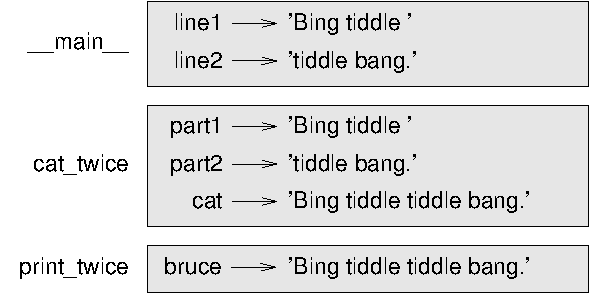
\includegraphics[scale=0.8]{figs/stack.pdf}}
\caption{แผนภาพแบบกองซ้อน (Stack diagram)}
\label{fig.stack}
\end{figure}


กรอบต่าง ๆ ถูกจัดวางเป็นกอง ๆ ซ้อนกัน โดยระบุว่าฟังก์ชันไหนเรียกฟังก์ชันไหน ไปเรื่อย ๆ
ในตัวอย่างนี้ ฟังก์ชัน \verb|print_twice| ถูกเรียกโดยฟังก์ชัน \verb|cat_twice| และ
ฟังก์ชัน \verb|cat_twice| ถูกเรียกเรียกโดยฟังก์ชัน \verb|__main__| ซึ่งเป็นชื่อพิเศษสำหรับเรียกกรอบ
ที่อยู่บนสุดของโปรแกรม เมื่อเราสร้างตัวแปรภายนอกฟังก์ชันอะไรก็ตาม มันจะถือว่าเป็นตัวแปรของส่วน \verb"__main__"
\index{main}
\index{โปรแกรมหลัก}

พารามิเตอร์แต่ละตัวอ้างอิงถึงค่าเดียวกันกับค่าของอาร์กิวเมนต์ที่ผ่านเข้ามา ณ ตำแหน่งเดียวกัน
ดังนั้น {\tt part1} มีค่าเดียวกันกับ {\tt line1}, {\tt part2} มีค่าเดียวกันกับ {\tt line2},
และ {\tt bruce} มีค่าเดียวกันกับ {\tt cat}

ถ้ามีข้อผิดพลาดเกิดขึ้นระหว่างที่มีการเรียกฟังก์ชัน ไพธอนจะพิมพ์ชื่อฟังก์ชันที่มีปัญหา ชื่อฟังก์ชันที่เรียกฟังก์ชันที่มีปัญหา 
และชื่อฟังก์ชันที่เรียกฟังก์ชัน {\em เมื่อกี้นี้} และย้อนกลับไปเรื่อย ๆ จนถึง \verb"__main__"

ตัวอย่างเช่น ถ้าเราพยายามที่จะเข้าถึง {\tt cat} จากในฟังก์ชัน \verb|print_twice| เราจะได้
ข้อผิดพลาดแบบทางชื่อ หรือ {\tt NameError}:

\begin{verbatim}
Traceback (innermost last):
  File "test.py", line 13, in __main__
    cat_twice(line1, line2)
  File "test.py", line 5, in cat_twice
    print_twice(cat)
  File "test.py", line 9, in print_twice
    print(cat)
NameError: name 'cat' is not defined
\end{verbatim}
%
รายชื่อฟังก์ชันเหล่านี้เรียกว่า {\bf การย้อนรอย (traceback)} มันบอกเราว่าโปรแกรมผิดพลาดที่ไฟล์ใด
บรรทัดใด และฟังก์ชันอะไรที่ทำงานอยู่ตอนนั้น  มันยังแสดงเลขบรรทัดของโค้ดที่เป็นเหตุของข้อผิดพลาดอีกด้วย
\index{traceback}
\index{การย้อนรอย}

ลำดับของฟังก์ชันต่าง ๆ ในการย้อนรอยเป็นลำดับเดียวกับลำดับของกรอบในแผนภาพแบบกองซ้อน
ฟังก์ชันที่กำลังทำงานอยู่จะอยู่ข้างล่างสุด 


\section{ฟังก์ชันที่ให้ผลและฟังก์ชันที่ไม่ให้ผล} % (Fruitful functions and void functions)}
\index{fruitful function}
\index{void function}
\index{function, fruitful}
\index{function, void} 
\index{ฟังก์ชันที่ให้ผล}
\index{ฟังก์ชัน void}
\index{ฟังก์ชัน, ที่ให้ผล}
\index{ฟังก์ชัน, void}

บางฟังก์ชันที่เราใช้กันมา เช่น ฟังก์ชันทางคณิตศาสตร์ มีการคืนผลลัพธ์กลับมาให้เรา  เนื่องจากไม่มีชื่อที่ดีกว่านี้
ผมจะเรียกพวกมันว่า {\bf ฟังก์ชันที่ให้ผล (fruitful functions)}  ส่วนฟังก์ชันอื่น ๆ จำพวกฟังก์ชัน 
\verb|print_twice| จะทำงานต่าง ๆ โดยไม่มีการคืนค่ากลับมา พวกมันเรียกว่า 
{\bf ฟังก์ชันที่ไม่ให้ผล หรือฟังก์ชันวอยด์ (void functions)} 

เมื่อเราเรียกฟังก์ชันที่ให้ผล เราต้องทำอะไรสักอย่างกับผลที่ได้คืนมานั้นเกือบจะเสมอ เช่น 
เราอาจจะกำหนดค่าของมันให้กับตัวแปร หรือใช้เป็นส่วนหนึ่งของนิพจน์:

\begin{verbatim}
x = math.cos(radians)
golden = (math.sqrt(5) + 1) / 2
\end{verbatim}
%
เมื่อเราเรียกฟังก์ชันในโหมดโต้ตอบ ไพธอนจะแสดงผลออกมา

\begin{verbatim}
>>> math.sqrt(5)
2.2360679774997898
\end{verbatim}
%
แต่ในโหมดสคริปต์ ถ้าเราเรียกฟังก์ชันที่มีผลแบบลอย ๆ ค่าผลลัพธ์ที่คืนกลับมาจะหายไปเลยชั่วนิรันดร์!

\begin{verbatim}
math.sqrt(5)
\end{verbatim}
% 
สคริปต์นี้คำนวณรากที่สองของ 5 แต่เนื่องจากมันไม่ได้เก็บค่าที่คืนกลับมาหรือแสดงค่าออกมา มันก็ไม่มีประโยชน์อะไรเท่าไหร่
\index{interactive mode}
\index{script mode}
\index{โหมดโต้ตอบ}
\index{โหมดสคริปต์}

ฟังก์ชันวอยด์อาจจะแสดงอะไรสักอย่างบนหน้าจอ หรือมีผลอย่างอื่น แต่มันไม่มีค่าที่ถูกส่งคืนกลับมา
ถ้าเรากำหนดค่าที่คืนกลับมาจากฟังก์ชันวอยด์ให้กับตัวแปร เราจะได้ค่าพิเศษที่เรียกว่า {\tt None}
\index{None special value}
\index{special value!None}
\index{ค่าพิเศษ None}
\index{ค่าพิเศษ!None}

\begin{verbatim}
>>> result = print_twice('Bing')
Bing
Bing
>>> print(result)
None
\end{verbatim}
%
ค่า {\tt None} ไม่ใช่ค่าเดียวกับสายอักขระ \verb"'None'" แต่มันเป็นค่าพิเศษที่มีชนิดของข้อมูลเป็นของมันเอง:

\begin{verbatim}
>>> type(None)
<class 'NoneType'>
\end{verbatim}
%
ฟังก์ชันที่เราเขียนกันมาถึงตอนนี้เป็นฟังก์ชันวอยด์ทั้งหมด เราจะเริ่มเขียนฟังก์ชันที่ให้ผลให้อีกสองสามบทถัดไป
\index{NoneType type}
\index{type!NoneType}
\index{ชนิด NoneType}
\index{ชนิด!NoneType}


\section{ทำไมต้องใช้ฟังก์ชัน} % (Why functions?)}
\index{function, reasons for}
\index{ฟังก์ชัน, เหตุผลในการใช้}

มันอาจจะไม่ชัดเจนเท่าไหร่ว่าทำไมมันถึงคุ้มค่ากับการปวดหัวเพื่อที่จะแบ่งโปรแกรมเป็นฟังก์ชันต่าง ๆ
มันมีเหตุผลหลายประการ ดังนี้:

\begin{itemize}

\item การสร้างฟังก์ชันใหม่สร้างโอกาสให้เราตั้งชื่อให้กลุ่มของคำสั่งได้ ทำให้โปรแกรมของเรานั้นอ่านและดีบักง่าย

\item ฟังก์ชันต่าง ๆ ทำให้โปรแกรมเล็กลงโดยการกำจัดโค้ดที่ซ้ำซ้อน  ในคราวหลัง ถ้าเราเปลี่ยนแปลงโค้ดพวกนั้น 
เราก็เพียงเปลี่ยนในที่เดียวเท่านั้น

\item การแบ่งโปรแกรมยาว ๆ ให้เป็นฟังก์ชันต่าง ๆ ทำให้เราดีบักได้ทีละส่วน จากนั้นเราก็
รวมส่วนต่าง ๆ เข้าด้วยกันให้มันทำงานได้แบบเต็มโปรแกรม

\item ฟังก์ชันที่ถูกออกแบบมาเป็นอย่างดีนั้นบ่อยครั้งจะมีประโยชน์กับหลายโปรแกรม เมื่อเราเขียนและดีบักครั้งหนึ่งแล้ว
เราสามารถใช้มันซ้ำได้ (ในโปรแกรมอื่น ๆ ด้วย)

\end{itemize}


\section{การดีบัก}

ทักษะที่สำคัญมากที่สุดอย่างหนึ่งที่เราจะได้เรียนรู้ คือ การตรวจแก้จุดบกพร่อง หรือการดีบัก (debugging)
ถึงแม้ว่ามันจะน่าท้อแท้อยู่สักหน่อย แต่การดีบักเป็นสิ่งที่ประเทืองปัญญา ท้าทาย 
และเป็นส่วนที่น่าสนใจของการเขียนโปรแกรม 

\index{experimental debugging}
\index{debugging!experimental}
\index{การดีบักแบบทดลอง}
\index{การดีบัก!แบบทดลอง}

ในบางแง่มุม การดีบักเหมือนกับงานสืบสวน เราจะเจอเบาะแสและเราจะต้องวินิจฉัยกระบวนการ
และเหตุการณ์ที่ทำให้เกิดผลลัพธ์แบบที่เราเห็นอยู่นี้ 

(หมายเหตุผู้แปล: คิดว่าผลนี้มันเกิดมาจากไหน ได้อย่างไร)

การดีบักยังเป็นเหมือนกับการทดลองทางวิทยาศาสตร์ เมื่อเรามีความคิดว่าอะไรที่น่าจะผิดพลาด เราจะแก้โปรแกรม
และลองดูอีก ถ้าสมมติฐานของเราถูก เราจะสามารถทำนายผลของการแก้ไขนั้นได้ และเราก็ได้ก้าวเข้าใกล้
โปรแกรมที่สามารถทำงานได้อีกก้าวหนึ่งแล้ว ถ้าสมมติฐานของเราผิด เราก็ต้องคิดสมมติฐานขึ้นมาใหม่
เป็นอย่างที่เชอร์ล็อค โฮล์มส์ชี้ให้เห็นว่า ``เมื่อเรากำจัดความเป็นไปไม่ได้แล้ว, อะไรก็ตามที่เหลือ, ไม่ว่ามันจะ
ดูเป็นไปไม่ได้ขนาดไหน, ก็จะต้องเป็นความจริง`` (A. Conan Doyle, {\em The Sign of Four})
\index{Holmes, Sherlock}
\index{Doyle, Arthur Conan}
\index{โฮล์มส์, เชอร์ล็อค}
\index{ดอลย์, อาเธอร์ โคนัน}

สำหรับบางคนแล้ว การเขียนโปรแกรมและการดีบักเป็นอย่างเดียวกัน นั่นคือ การเขียนโปรแกรมเป็นกระบวนการของการ
ค่อย ๆ ดีบักโปรแกรมจนกว่ามันจะทำสิ่งที่เราต้องการได้ หลักการคือ เราควรจะเริ่มจากโปรแกรมเล็ก ๆ ที่ทำงานได้
และแก้ไขไปทีละน้อย นั่นคือการดีบักไปพร้อมกับการเขียนโปรแกรม 

(หมายเหตุผู้แปล: เขียนเพิ่มและดีบักเพิ่มทีละเล็กทีละน้อย)

ตัวอย่างเช่น ลินิกซ์ (Linux) เป็นระบบปฏิบัติการที่มีโค้ดเป็นล้าน ๆ บรรทัด แต่มันเริ่มมาจากโปรแกรมเล็ก ๆ ที่
ลินัส ทอร์วัลด์ส (Linus Torvalds) ใช้สำรวจชิป Intel 80386  จากคำบอกเล่าของ
ลาร์รี กรีนฟิลด์ (Larry Greenfield) ``โครงงานแรก ๆ ของลินัส คือ โปรแกรมที่จะสับเปลี่ยนระหว่างการพิมพ์
AAAA และ BBBB โปรแกรมนี้ได้วิวัฒนาการมาเป็นลินิกซ์'' ({\em The Linux Users' Guide} Beta Version 1)
\index{Linux}
\index{ลินิกซ์}


\section{อภิธานศัพท์}

\begin{description}

\item[ฟังก์ชัน (function):] ลำดับของคำสั่งที่มีชื่อเรียก ซึ่งทำงานอะไรสักอย่างที่มีประโยชน์ 
ฟังก์ชันอาจจะรับหรือไม่รับอาร์กิวเมนต์ และอาจจะมีผลลัพธ์หรือไม่ก็ได้
\index{function} 
\index{ฟังก์ชัน}

\item[นิยามฟังก์ชัน (function definition):] คำสั่งที่ใช้สร้างฟังก์ชันใหม่ โดยระบุชื่อ พารามิเตอร์
และคำสั่งที่อยู่ในฟังก์ชัน  
\index{function definition}
\index{นิยามฟังก์ชัน}

\item[วัตถุฟังก์ชัน (function object):] ค่าที่ถูกสร้างโดยนิยามฟังก์ชัน ชื่อฟังก์ชันคือตัวแปรที่อ้างอิงถึงวัตถุฟังก์ชัน 
\index{function object}
\index{วัตถุฟังก์ชัน}

\item[ส่วนหัว (header):] บรรทัดแรกของนิยามฟังก์ชัน
\index{header}
\index{ส่วนหัว}

\item[ส่วนตัว (body):] กลุ่มลำดับของคำสั่งที่อยู่ในนิยามฟังก์ชัน
\index{body}
\index{ส่วนตัว}

\item[พารามิเตอร์ (parameter):] ชื่อที่ถูกใช้ในฟังก์ชันเพื่ออ้างอิงถึงค่าที่ถูกผ่านเข้ามาเป็นอาร์กิวเมนต์
\index{parameter}
\index{พารามิเตอร์ }

\item[การเรียกฟังก์ชัน (function call):] คำสั่งที่ทำให้ฟังก์ชันทำงาน ประกอบด้วย ชื่อฟังก์ชัน ตามด้วยรายการ
อาร์กิวเมนต์ในวงเล็บ
\index{function call}
\index{การเรียกฟังก์ชัน }

\item[อาร์กิวเมนต์ (argument):] ค่าที่ส่งผ่านไปให้ฟังก์ชันเมื่อฟังก์ชันถูกเรียกใช้งาน ค่านี้ถูกกำหนดให้กับพารามิเตอร์ที่
ตรงตำแหน่งกันในฟังก์ชัน 
\index{argument}
\index{อาร์กิวเมนต์}

\item[ตัวแปรเฉพาะที่ (local variable):] ตัวแปรที่ถูกนิยามขึ้นภายในฟังก์ชัน ตัวแปรเฉพาะที่สามารถถูกใช้งานได้
ภายในฟังก์ชันของมันเท่านั้น 
\index{local variable}
\index{ตัวแปรเฉพาะที่}

\item[ค่าคืนกลับ (return value):] ผลลัพธ์ของฟังก์ชัน ถ้าการเรียกฟังก์ชันนั้นถูกใช้เป็นนิพจน์
ค่าคืนกลับจะกลายมาเป็นค่าของนิพจน์นั้นเลย
\index{return value}
\index{ค่าคืนกลับ}

\item[ฟังก์ชันที่ให้ผล (fruitful function):] ฟังก์ชันที่คืนค่ากลับมา
\index{fruitful function}
\index{ฟังก์ชันที่ให้ผล}

\item[ฟังก์ชันที่ไม่ให้ผล หรือ ฟังก์ชันวอยด์ (void function):] ฟังก์ชันที่คืนค่ากลับมาเป็น {\tt None} เสมอ
\index{void function}
\index{ฟังก์ชัน void}

\item[{\tt None}:] ค่าพิเศษที่ถูกคืนกลับมาโดยฟังก์ชันวอยด์
\index{None special value}
\index{special value!None}
\index{ค่าพิเศษ None}
\index{ค่าพิเศษ!None}

\item[มอดูล (module):] ไฟล์ที่บรรจุฟังก์ชันและนิยามต่าง ๆ ที่เกี่ยวข้องกัน 
\index{module}
\index{มอดูล}

\item[คำสั่งนำเข้า (import statement):] คำสั่งที่อ่านไฟล์มอดูลและสร้างวัตถุมอดูล
\index{import statement}
\index{statement!import}
\index{คำสั่งนำเข้า}
\index{คำสั่ง!นำเข้า}

\item[วัตถุมอดูล (module object):] ค่าที่ถูกสร้างขึ้นโดยคำสั่ง {\tt import} 
ที่เอื้อให้สามารถเข้าถึงค่าที่ถูกนิยามในมอดูล
\index{module object}
\index{วัตถุมอดูล}

\item[สัญกรณ์จุด (dot notation):]  กฎวากยสัมพันธ์สำหรับเรียกฟังก์ชันในมอดูลอื่น ซึ่งให้ระบุชื่อของมอดูล
ตามด้วยเครื่องหมายจุดและชื่อฟังก์ชันที่ต้องการเรียก 
\index{dot notation}
\index{สัญกรณ์จุด}

\item[การประกอบ (composition):] การใช้นิพจน์เป็นส่วนประกอบของนิพจน์อีกอันที่ใหญ่กว่า 
หรือคำสั่งที่เป็นส่วนประกอบของอีกคำสั่งที่ใหญ่กว่า
\index{composition}
\index{การประกอบ}

\item[กระแสการดำเนินการ (flow of execution):]  ลำดับการทำงานของคำสั่งต่าง ๆ
\index{flow of execution}
\index{กระแสการดำเนินการ}

\item[แผนภาพแบบกองซ้อน (stack diagram):]  การใช้รูปภาพแสดงกองของฟังก์ชัน ตัวแปรของแต่ละฟังก์ชัน 
และค่าที่ถูกอ้างถึง
\index{stack diagram}
\index{แผนภาพแบบกองซ้อน}

\item[กรอบ (frame):]  กล่องในแผนภาพแบบกองซ้อนที่แสดงการเรียกฟังก์ชันหนึ่ง ๆ ซึ่งประกอบด้วยตัวแปรเฉพาะที่
และพารามิเตอร์ของฟังก์ชัน
\index{function frame}
\index{frame}
\index{กรอบฟังก์ชัน}
\index{กรอบ}

\item[การย้อนรอย (traceback):]  รายการของฟังก์ชันต่าง ๆ ที่ทำงานอยู่ โดยจะถูกพิมพ์ออกมาเมื่อเกิดข้อยกเว้น
(ความผิดพลาดตอนโปรแกรมทำงาน)
\index{traceback}
\index{การย้อนรอย}


\end{description}


\section{แบบฝึกหัด}

\begin{exercise}
\index{len function}
\index{function!len}
\index{ฟังก์ชัน len}
\index{ฟังก์ชัน!len}

ให้เขียนฟังก์ชันที่ชื่อว่า \verb"right_justify" ซึ่งรับสายอักขระที่ชื่อว่า {\tt s} เป็นพารามิเตอร์ และพิมพ์
สายอักขระดังกล่าวโดยมีช่องว่างนำหน้า แล้วทำให้อักษรตัวสุดท้ายของสายอักขระอยู่ในหลักที่ 70 ของการแสดงผล 

\begin{verbatim}
>>> right_justify('monty')
                                                                 monty
\end{verbatim}

คำใบ้: ใช้การเชื่อมต่อสายอักขระและการทำซ้ำ นอกจากนี้ ไพธอนได้เตรียมฟังก์ชันที่ชื่อว่า {\tt len} ซึ่งจะคืนค่า
ความยาวของสายอักขระ ดังนั้น ค่าของ \verb"len('monty')" คือ 5

\end{exercise}


\begin{exercise}
\index{function object}
\index{object!function}
\index{วัตถุฟังก์ชัน}
\index{วัตถุ!ฟังก์ชัน}

วัตถุฟังก์ชัน คือ ค่าที่เราสามารถกำหนดให้กับตัวแปร หรือผ่านเข้าไปเป็นอาร์กิวเมนต์
เช่น ฟังก์ชัน \verb"do_twice" เป็นฟังก์ชันที่รับวัตถุฟังก์ชันเป็นอาร์กิวเมนต์ และเรียกฟังก์ชันนั้นสองรอบ 
(ฟังก์ชัน f() จะทำงาน 2 ครั้ง)

\begin{verbatim}
def do_twice(f):
    f()
    f()
\end{verbatim}

นี่คือตัวอย่างที่ใช้ฟังก์ชัน \verb"do_twice" เพื่อเรียกฟังก์ชัน \verb|print_spam| ให้ทำงานสองครั้ง 

\begin{verbatim}
def print_spam():
    print('spam')

do_twice(print_spam)
\end{verbatim}

\begin{enumerate}

\item ให้เขียนตัวอย่างนี้ลงในสคริปต์ และทดสอบโปรแกรมดู

\item ให้แก้ไขฟังก์ชัน \verb"do_twice" ให้รับอาร์กิวเมนต์เข้ามา 2 ตัว เป็นวัตถุฟังก์ชัน 1 ตัว และค่า 1 ค่า
ให้เรียกฟังก์ชันที่รับเข้ามา 2 รอบ โดยผ่านอีกค่าที่รับเข้ามาเป็นอาร์กิวเมนต์ของฟังก์ชันดังกล่าว

\item ให้คัดลอกนิยามของฟังก์ชัน \verb|print_twice| จากก่อนหน้านี้ในบทนี้แล้วใส่ในสคริปต์ของเรา

\item ให้ใช้ฟังก์ชัน \verb"do_twice" ที่แก้ไขไปก่อนหน้านี้เพื่อเรียกฟังก์ชัน \verb|print_twice| สองครั้ง
โดยให้ผ่าน \verb"'spam'" เป็นอาร์กิวเมนต์

\item ให้นิยามฟังก์ชันใหม่ที่ชื่อว่า \verb"do_four" ซึ่งรับวัตถุฟังก์ชัน 1 ตัว และค่า 1 ค่า
และเรียกฟังก์ชันที่รับเข้ามา 4 รอบโดยผ่านอีกค่าที่รับเข้ามาเป็นพารามิเตอร์
จะต้องมีคำสั่งแค่ 2 คำสั่งเท่านั้นในตัวฟังก์ชันนี้ ไม่ใช่ 4 คำสั่ง

\end{enumerate}

เฉลย: \url{http://thinkpython2.com/code/do_four.py}.

\end{exercise}



\begin{exercise}

หมายเหตุ: ข้อนี้จะต้องใช้คำสั่งและลักษณะเฉพาะที่เราเรียนมาจนถึงตอนนี้เท่านั้น  

\begin{enumerate}

\item ให้เขียนฟังก์ชันที่วาดรูปตารางดังต่อไปนี้
\index{grid}
\index{ตาราง}

\begin{verbatim}
+ - - - - + - - - - +
|         |         |
|         |         |
|         |         |
|         |         |
+ - - - - + - - - - +
|         |         |
|         |         |
|         |         |
|         |         |
+ - - - - + - - - - +
\end{verbatim}
% 
คำใบ้: ในการพิมพ์ค่ามากกว่า 1 ค่าบนหนึ่งบรรทัด เราสามารถพิมพ์ค่าหลายค่าต่อกันโดยคั่นด้วยเครื่องหมายจุลภาค (,):

\begin{verbatim}
print('+', '-')
\end{verbatim}
%
คำสั่ง {\tt print} ขึ้นบรรทัดใหม่โดยปริยาย แต่เราสามารถยกเลิกพฤติกรรมนี้
และใส่ช่องว่างในตอนท้ายของการพิมพ์ได้ โดยทำแบบนี้:

\begin{verbatim}
print('+', end=' ')
print('-')
\end{verbatim}
%
ผลของคำสั่งเหล่านี้ คือ \verb"'+ -'"

คำสั่ง {\tt print} ที่ไม่มีอาร์กิวเมนต์จะจบบรรทัดปัจจุบันและขึ้นบรรทัดใหม่

\item ให้เขียนฟังก์ชันที่วาดรูปตารางแบบรูปที่แล้ว แต่ให้มี 4 แถวและ 4 หลัก

\end{enumerate}

เฉลย: \url{http://thinkpython2.com/code/grid.py}.
ที่มา: แบบฝึกหัดข้อนี้ดัดแปลงมาจากแบบฝึกหัดใน Oualline, {\em
Practical C Programming, Third Edition}, O'Reilly Media, 1997.

\end{exercise}




\chapter{กรณีศึกษา การออกแบบส่วนต่อประสานงาน }%(interface design)}
\label{turtlechap}

บทนี้นำเสนอกรณีศึกษาที่สาธิตขั้นตอนการออกแบบฟังก์ชันต่าง ๆ ที่ทำงานร่วมกัน

บทนี้แนะนำมอดูล {\tt turtle} ที่ทำให้เราสามารถสร้างรูปภาพโดยใช้กราฟิกเต่า (turtle graphics)
มอดูล {\tt turtle} มากับการติดตั้งภาษาไพธอนส่วนมากอยู่แล้ว แต่ถ้าเราใช้ไพธอนของ PythonAnywhere
เราจะไม่สามารถรันตัวอย่างในมอดูล turtle ได้ (อย่างน้อยก็ยังไม่ได้ในตอนที่ผมเขียนหนังสือเล่มนี้)

ถ้าเราลงไพธอนบนคอมพิวเตอร์ของเราแล้ว เราจะสามารถรันตัวอย่างในมอดูล turtle ได้ ไม่เช่นนั้น ตอนนี้ก็เป็น
เวลาที่ดีนะที่จะติดตั้งไพธอน  ผมได้โพสต์ขั้นตอนการติดตั้งไว้ที่ \url{http://tinyurl.com/thinkpython2e}

ตัวอย่างของโค้ดที่ใช้ในบทนี้ อยู่ที่ \url{http://thinkpython2.com/code/polygon.py}

หมายเหตุผู้แปล: ในบทนี้จะใช้คำว่า turtle แทนคำว่า เต่า เพราะเป็นชื่อเฉพาะ

\section{มอดูล turtle} % (The turtle module)}
\label{turtle}

ในการตรวจสอบว่าเรามีมอดูล {\tt turtle} ในเครื่องหรือเปล่า ให้เปิดตัวแปลภาษาไพธอนขึ้นมาแล้วพิมพ์

\begin{verbatim}
>>> import turtle
>>> bob = turtle.Turtle()
\end{verbatim}

เมื่อเรารันโค้ดนี้แล้ว ไพธอนควรจะสร้างหน้าต่างใหม่ขึ้นมาพร้อมกับลูกศรเล็ก ๆ ที่เป็นตัวแทนของ turtle
ถ้าได้แล้วก็ปิดหน้าต่างได้

ให้สร้างไฟล์ชื่อว่า {\tt mypolygon.py} และพิมพ์โค้ดต่อไปนี้:

\begin{verbatim}
import turtle
bob = turtle.Turtle()
print(bob)
turtle.mainloop()
\end{verbatim}
%
มอดูล {\tt turtle} (เขียนด้วย 't' ตัวเล็ก) ได้เตรียมฟังก์ชันชื่อว่า {\tt Turtle} (เขียนด้วย 'T' ตัวใหญ่) 
ซึ่งสร้างวัตถุ Turtle ที่เรากำหนดให้กับตัวแปรที่ชื่อว่า {\tt bob} การพิมพ์ {\tt bob} ออกมาจะแสดงผลประมาณนี้:

\begin{verbatim}
<turtle.Turtle object at 0xb7bfbf4c>
\end{verbatim}
%
นี่หมายความว่า {\tt bob} อ้างอิงถึงวัตถุชนิด {\tt Turtle} อย่างที่ถูกนิยามในมอดูล {\tt turtle} นั่นเอง

ฟังก์ชัน \verb"mainloop" สั่งให้หน้าต่างที่เปิดขึ้นมารอให้ผู้ใช้ทำอะไรสักอย่าง แม้ว่าในกรณีนี้ มันไม่มีอะไร
ให้ผู้ใช้ทำมากนัก ยกเว้นการปิดหน้าต่าง

เมื่อเราสร้างวัตถุชนิด Turtle แล้ว เราสามารถเรียก {\bf เมธอด (method)} เพื่อจะเลื่อนมันไปรอบ ๆ หน้าต่างได้
เมธอดเป็นเหมือนฟังก์ชัน แต่มันใช้กฎวากยสัมพันธ์ในการเขียนที่ต่างไปนิดหน่อย เช่น 
เมื่อเราต้องการจะเลื่อนเต่าไปข้างหน้า:

\begin{verbatim}
bob.fd(100)
\end{verbatim}
%
เมธอด  {\tt fd} มีความเชื่อมโยงกับวัตถุ turtle ที่เรียกว่า {\tt bob} การเรียกใช้งานเมธอดเหมือนกับ
การขอร้อง: เราขอให้ {\tt bob} เคลื่อนที่ไปข้างหน้า

อาร์กิวเมนต์ของเมธอด {\tt fd} คือ ระยะทางในหน่วยพิกเซล (pixel) ดังนั้น ขนาดของการเคลื่อนที่จะขึ้น
อยู่กับจอของแต่ละคน

เมธอดอื่นที่เราสามารถเรียกใช้กับ Turtle ได้ คือ {\tt bk} เพื่อที่จะเคลื่อนไปข้างหลัง, {\tt lt} เพื่อเลี้ยวซ้าย, 
และ {\tt rt} เพื่อเลี้ยวขวา อาร์กิวเมนต์ของ {\tt lt} และ {\tt rt} เป็นขนาดของมุมในหน่วยองศา (degree)

นอกจากนี้ Turtle แต่ละตัวจะถือปากกาของมันเอง ซึ่งจะจรดลง (down) หรือ ยกขึ้น (up); 
ถ้า Turtle จรดปากกาลงมันจะทิ้งรอยขีดไว้เมื่อมันเคลื่อนที่  เมธอด {\tt pu} และ {\tt pd} 
เป็นตัวย่อของ ``pen up' (ยกปากกาขึ้น) และ ``pen down'' (จรดปากกาลง)

เพื่อที่จะวาดมุมที่ถูกต้อง ให้เพิ่มบรรทัดเหล่านี้เข้าไปในโปรแกรม หลังจากสร้าง {\tt bob} แล้ว
แต่ใส่ก่อนที่จะเรียกฟังก์ชัน \verb"mainloop":

\begin{verbatim}
bob.fd(100)
bob.lt(90)
bob.fd(100)
\end{verbatim}
%
เมื่อเรารันโปรแกรมนี้ เราควรจะเห็น {\tt bob} เคลื่อนที่ไปทางทิศตะวันออก และจากนั้นไปทางทิศเหนือ
โดยที่ทิ้งเส้นไว้สองส่วน

คราวนี้ ให้แก้ไขโปรแกรมเพื่อจะวาดรูปสี่เหลี่ยมจตุรัส อย่าเพิ่งทำอย่างอื่นต่อจนกว่าจะวาดได้!

%\newpage

\section{การทำซ้ำแบบง่าย ๆ}% (Simple repetition)}
\label{repetition}
\index{repetition}
\index{การทำซ้ำ}

เราอาจจะเขียนโปรแกรมเมื่อกี้ออกมาประมาณนี้:

\begin{verbatim}
bob.fd(100)
bob.lt(90)

bob.fd(100)
bob.lt(90)

bob.fd(100)
bob.lt(90)

bob.fd(100)
\end{verbatim}
%
%We can do the same thing more concisely with a {\tt for} statement.
%Add this example to {\tt mypolygon.py} and run it again:
เราสามารถทำสิ่งที่เหมือนกันแต่กระชับกว่า โดยการใช้คำสั่ง {\tt for}  ให้เพิ่มตัวอย่างนี้เข้าไปในไฟล์ 
{\tt mypolygon.py} แล้วลองรันดูอีกที
\index{for loop}
\index{loop!for}
\index{statement!for}
\index{ลูป for}
\index{ลูป!for}
\index{คำสั่ง!for}

\begin{verbatim}
for i in range(4):
    print('Hello!')
\end{verbatim}
%
แล้วเราควรจะเห็นผลประมาณนี้:

\begin{verbatim}
Hello!
Hello!
Hello!
Hello!
\end{verbatim}
%
นี่เป็นการใช้งานที่ง่ายที่สุดของคำสั่ง {\tt for}; เราจะเห็นตัวอย่างอีกมากในภายหลัง 
แต่ตัวอย่างนี้ก็น่าจะเพียงพอสำหรับการให้เราเขียนโปรแกรมวาดรูปสี่เหลี่ยมใหม่ 
อย่าเพิ่งทำอย่างอื่นต่อจนกว่าจะทำได้นะ

นี่เป็นคำสั่ง {\tt for} ที่วาดรูปสี่เหลี่ยมจตุรัส:

\begin{verbatim}
for i in range(4):
    bob.fd(100)
    bob.lt(90)
\end{verbatim}
%
กฎวากยสัมพันธ์ของคำสั่ง {\tt for} นั้นเหมือนกับของฟังก์ชัน มันจะมีส่วนหัวที่ลงท้ายด้วยทวิภาค (:)
และส่วนตัวที่ต้องย่อหน้าเข้าไป ส่วนตัวของ for สามารถมีคำสั่งอยู่ภายในได้กี่คำสั่งก็ได้

คำสั่ง {\tt for} นี้สามารถเรียกว่า {\bf ลูป (loop)} ได้ด้วย เนื่องจากกระแสการดำเนินการ 
(flow of execution) ทำงานผ่านไปตามส่วนตัวของคำสั่ง จากนั้นมันจะวนกลับไปทำคำสั่งบนสุดของคำสั่ง for  
ในกรณีนี้ โปรแกรมจะรันคำสั่งในส่วนตัวเป็นจำนวน 4 ครั้ง 
\index{loop}
\index{ลูป}

โค้ดเวอร์ชันนี้แตกต่างจากโค้ดวาดรูปสี่เหลี่ยมจตุรัสอันที่แล้วนิดหน่อย เพราะว่ามันหันข้างหลังจาก
วาดเส้นสุดท้ายของสี่เหลี่ยมจตุรัสแล้ว การหันข้างที่เพิ่มขึ้นมานี้ใช้เวลามากขึ้น แต่ว่ามันทำให้โค้ดง่ายขึ้นถ้าเราจะทำ
สิ่งที่เหมือน ๆ กันทุกครั้งที่ทำลูป โค้ดเวอร์ชันนี้ยังทำให้ turtle มันกลับไปที่จุดเริ่มต้น
และหันหน้ากลับไปในทางเดียวกับตอนเริ่มต้นด้วย


\section{แบบฝึกหัด}

ต่อไปนี้จะเป็นชุดแบบฝึกหัดที่ใช้ TurtleWorld มันน่าจะสนุกแต่ก็มีประเด็นความรู้ด้วย
ในระหว่างที่เราทำแบบฝึกหัดนี้ ให้คิดว่าประเด็นความรู้ที่ได้คืออะไร

หัวข้อต่อไปนี้มีเฉลยของแบบฝึกหัดด้วย ดังนั้น ห้ามไปดูเฉลยจนกว่าเราจะทำเสร็จ 
(หรืออย่างน้อยก็พยายามทำก่อน)

\begin{enumerate}

\item ให้เขียนฟังก์ชันที่ชื่อว่า {\tt square} ซึ่งรับพารามิเตอร์ชื่อว่า {\tt t} ที่เป็น turtle 
ฟังก์ชันนี้ควรจะใช้ turtle ในการวาดสี่เหลี่ยมจัตุรัส

ให้เขียนการเรียกฟังก์ชันที่ผ่านค่า {\tt bob} เข้าไปเป็นอาร์กิวเมนต์สำหรับฟังก์ชัน {\tt square}
จากนั้นให้รันโปรแกรมอีกทีหนึ่ง

\item ให้เพิ่มพารามิเตอร์อีกหนึ่งตัว ชื่อว่า {\tt length} เข้าไปยัง {\tt square}
ทำการแก้ไขส่วนตัวของฟังก์ชันโดยให้ความยาวของด้านคือ {\tt length} จากนั้นให้แก้ไขการเรียกฟังก์ชัน
โดยให้ผ่านอาร์กิวเมนต์ตัวที่สองเข้าไปด้วย รันโปรแกรมอีกครั้งหนึ่ง ทดสอบโปรแกรมกับค่า {\tt length}
ในช่วงค่าต่าง ๆ

\item ให้คัดลอกฟังก์ชัน {\tt square} แล้วเปลี่ยนชื่อเป็น {\tt polygon}
เพิ่มพารามิเตอร์อีกตัวชื่อว่า {\tt n} ทำการแก้ไขส่วนตัวของฟังก์ชันให้วาดรูป n เหลี่ยมด้านเท่า 
(รูปหลายเหลี่ยมด้านเท่าที่มี n ด้าน)
คำใบ้: มุมภายนอกของรูป n เหลี่ยมด้านเท่า คือ $360/n$ องศา  
\index{polygon function} \index{function!polygon}
\index{ฟังก์ชันรูปหลายเหลี่ยม} \index{ฟังก์ชัน!รูปหลายเหลี่ยม}

\item ให้เขียนฟังก์ชันที่ชื่อว่า {\tt circle} ซึ่งรับ turtle {\tt t}, และรัศมี {\tt r} เป็นพารามิเตอร์
และวาดวงกลมกลาย ๆ โดยการเรียกฟังก์ชัน {\tt polygon} ด้วยความยาวและจำนวนด้านที่เหมาะสม
ทดสอบฟังก์ชันของเราด้วยช่วงค่า {\tt r} ต่าง ๆ
\index{circle function} \index{function!circle}
\index{ฟังก์ชันวงกลม} \index{ฟังก์ชัน!วงกลม}

คำใบ้: ลองหาเส้นรอบวง (circumference) ของวงกลม และทำให้ {\tt length * n = circumference}

\item ให้สร้างฟังก์ชัน {\tt circle} ที่จะสามารถใช้ครอบคลุมกรณีอื่น ๆ ได้ โดยให้ชื่อว่า {\tt arc}
ซึ่งรับพารามิเตอร์อีกตัวหนึ่ง คือ {\tt angle} ซึ่งกำหนดสัดส่วนของวงกลมที่เราจะวาด
{\tt angle} มีหน่วยเป็นองศา (degree)  ดังนั้น เมื่อ {\tt angle=360} ฟังก์ชัน {\tt arc} 
ควรจะวาดวงกลมที่สมบูรณ์

\index{arc function}
\index{function!arc}
\index{ฟังก์ชันเส้นโค้ง}
\index{ฟังก์ชัน!เส้นโค้ง}

\end{enumerate}


\section{การห่อหุ้ม} % (Encapsulation)}

แบบฝึกหัดแรกให้เรานำโค้ดวาดรูปสี่เหลี่ยมจัตุรัสมาใส่ในนิยามฟังก์ชัน และจากนั้นเรียกฟังก์ชัน
โดยผ่าน turtle เป็นพารามิเตอร์  นี่คือเฉลย:

\begin{verbatim}
def square(t):
    for i in range(4):
        t.fd(100)
        t.lt(90)

square(bob)
\end{verbatim}
%
คำสั่งชุดข้างในสุด (ย่อหน้าในสุด), {\tt fd} และ {\tt lt}, ถูกย่อหน้าเข้าไปสองรอบ 
เพื่อแสดงให้เห็นว่าพวกมันอยู่ใน {\tt for} ลูป ซึ่งอยู่ในนิยายของฟังก์ชันอีกที
บรรทัดถัดมา, {\tt square(bob)}, ถูกล้างขอบซ้าย (เว้นบรรทัดและกลับเข้าไปชิดขอบซ้ายสุด)
ซึ่งระบุถึงการสิ้นสุดของทั้งลูป {\tt for} และนิยามฟังก์ชัน

ในฟังก์ชันนี้ ตัวแปร {\tt t} อ้างอิงถึง turtle ตัวเดียวกับ {\tt bob}  ดังนั้น คำสั่ง {\tt t.lt(90)}
จะให้ผลเหมือนกับคำสั่ง {\tt bob.lt(90)}  ในกรณีนี้ แล้วทำไมเราไม่เรียกพารามิเตอร์ว่า {\tt bob} ล่ะ?
หลักการคือ {\tt t} สามารถเป็น turtle ตัวไหนก็ได้ ไม่เฉพาะแค่ {\tt bob} เท่านั้น  ดังนั้น เราสามารถ
สร้าง turtle ตัวที่สอง และผ่านมันเป็นอาร์กิวเมนต์เข้าไปยังฟังก์ชัน {\tt square} ได้:

\begin{verbatim}
alice = turtle.Turtle()
square(alice)
\end{verbatim}
%
การห่อชิ้นส่วนของโค้ดในฟังก์ชันนั้นเรียกว่า {\bf การห่อหุ้ม (encapsulation)}
ประโยชน์ของการห่อหุ้มอย่างหนึ่ง คือ มันจะผูกโค้ดเหล่านั้นไว้กับชื่อชื่อหนึ่ง ซึ่งทำหน้าที่คล้ายการบันทึกเอกสารด้วย
ประโยชน์อีกอย่าง คือ การที่เราสามารถใช้โค้ดนี้ซ้ำได้ มันกระชับมากกว่าเมื่อเราเรียกฟังก์ชันซ้ำสองครั้ง แทนที่จะ
คัดลอกโค้ดและเอามาวาง (copy and paste)
\index{encapsulation}
\index{การห่อหุ้ม}


\section{การทำให้ครอบคลุม} % (Generalization)}

ขั้นตอนถัดไป คือ การเพิ่มพารามิเตอร์ {\tt length} ให้กับฟังก์ชัน {\tt square} 
นี่คือเฉลย:

\begin{verbatim}
def square(t, length):
    for i in range(4):
        t.fd(length)
        t.lt(90)

square(bob, 100)
\end{verbatim}
%
การเพิ่มพารามิเตอร์ให้ฟังก์ชันนั้นเรียกว่า {\bf การทำให้ครอบคลุม (generalization)}
เพราะว่ามันทำให้ฟังก์ชันนั้นทำงานแบบครอบคลุมกรณีทั่วไปมากยิ่งขึ้น: ในเวอร์ชันก่อนหน้า 
สี่เหลี่ยมจตุรัสนั้นมีขนาดเดิมเสมอ; แต่ในเวอร์ชันนี้ มันสามารถเป็นขนาดอะไรก็ได้
\index{generalization}
\index{การทำให้ครอบคลุม}

ขั้นตอนถัดไปก็เป็นการทำให้ครอบคลุมเช่นกัน แทนที่เราจะวาดสี่เหลี่ยมจตุรัส  ฟังก์ชัน {\tt polygon} 
วาดรูปหลายเหลี่ยมด้านเท่า โดยมีจำนวนด้านเท่าไหร่ก็ได้ 
นี่คือเฉลย:

\begin{verbatim}
def polygon(t, n, length):
    angle = 360 / n
    for i in range(n):
        t.fd(length)
        t.lt(angle)

polygon(bob, 7, 70)
\end{verbatim}
%

ตัวอย่างนี้วาดรูป 7 เหลี่ยมที่มีด้านยาว 70 
(หมายเหตุผู้แปล: หน่วยเป็นพิกเซล)

ถ้าเราใช้ไพธอน 2 ค่าของ {\tt angle} อาจจะเพี้ยน ๆ หน่อย เพราะเป็นการหารของจำนวนเต็ม 
ทางแก้ง่าย ๆ คือการคำนวณเป็น {\tt angle = 360.0 / n} เพราะว่าตัวเศษเป็นเลขจุดลอย 
ค่าผลลัพธ์ที่ได้ก็จะเป็นค่าจุดลอย

(หมายเหตุผู้แปล: ในการทำ integer division นั้นจำนวนเต็มหารจำนวนเต็มจะได้ค่าผลลัพธ์เป็นจำนวนเต็ม)
\index{Python 2}
\index{ไพธอน 2}

เมื่อฟังก์ชันมีจำนวนอาร์กิวเมนต์มากกว่า 2-3 ตัว มันง่ายที่จะลืมว่าแต่ละตัวคืออะไร 
หรือลำดับในการวางควรเป็นอย่างไร  ในกรณีดังกล่าว มันเป็นความคิดที่ดีที่จะใส่ชื่อ
ของพารามิเตอร์ในลิสต์ของอาร์กิวเมนต์:

\begin{verbatim}
polygon(bob, n=7, length=70)
\end{verbatim}
%
อาร์กิวเมนต์แบบนี้เรียกว่า {\bf อาร์กิวเมนต์คำสำคัญ (keyword arguments)} เพราะว่ามันใส่ชื่อ
ของพารามิเตอร์ลงไปเป็น ``คำสำคัญ (keywords)'' (อย่าสับสนกับคำสำคัญของไพธอน เช่น 
{\tt while} และ {\tt def})
\index{keyword argument}
\index{argument!keyword}
\index{อาร์กิวเมนต์คำสำคัญ}
\index{อาร์กิวเมนต์!คำสำคัญ}

กฎวากยสัมพันธ์นี้ทำให้เราสามารถอ่านโปรแกรมได้ง่ายขึ้น มันยังเตือนให้เรารู้ว่าอาร์กิวเมนต์และ
พารามิเตอร์ทำงานอย่างไร: เมื่อเราเรียกฟังก์ชัน อาร์กิวเมนต์จะถูกกำหนดค่าให้กับพารามิเตอร์


\section{การออกแบบส่วนต่อประสานงาน} % (Interface design)}

ขั้นต่อไปคือการเขียนฟังก์ชัน {\tt circle} ซึ่งรับรัศมี (radius) {\tt r} เป็นพารามิเตอร์
นี่คือเฉลยง่าย ๆ ที่ใช้ฟังก์ชัน {\tt polygon} ในการวาดรูป 50 เหลี่ยมด้านเท่า:

\begin{verbatim}
import math

def circle(t, r):
    circumference = 2 * math.pi * r
    n = 50
    length = circumference / n
    polygon(t, n, length)
\end{verbatim}
%
บรรทัดแรกคำนวณเส้นรอบวงของวงกลมที่มีรัศมี {\tt r} โดยใช้สูตร $2 \pi r$ เนื่องจากเราใช้ {\tt math.pi}
เราต้องนำเข้ามอดูล {\tt math} ด้วย โดยปกติแล้ว คำสั่ง {\tt import} จะอยู่ในตอนเริ่มต้นของไฟล์สคริปต์

{\tt n} คือ จำนวนเส้นในการวาดวงกลมโดยประมาณของเรา และ {\tt length} คือ ความยาวของแต่ละเส้นนั้น  
ดังนั้น ฟังก์ชัน {\tt polygon} วาดรูปหลายเหลี่ยมจำนวน 50 เหลี่ยม เพื่อจะประมาณการเป็นวงกลมที่มีรัศมี {\tt r}

ข้อจำกัดของเฉลยแบบนี้คือ {\tt n} เป็นค่าคงที่ หมายถึงว่าสำหรับวงกลมอันใหญ่ ๆ แล้ว เส้นที่วาดนี้มันจะยาวเกินไป
และสำหรับวงกลมเล็ก ๆ นี้ เราจะเสียเวลาวาดเส้นน้อย ๆ หลาย ๆ เส้น ทางแก้ทางหนึ่งคือการทำฟังก์ชันให้ครอบคลุม (generalize)
โดยการเอา {\tt n} มาเป็นพารามิเตอร์ มันจะทำให้ผู้ใช้ (หรือใครก็ตามที่เรียกฟังก์ชัน {\tt circle}) สามารถควบคุม
การใช้งานได้ดีขึ้น แต่ส่วนต่อประสานงาน (interface) จะเรียบร้อยน้อยลง
\index{interface}
\index{ส่วนต่อประสานงาน}

{\bf ส่วนต่อประสานงาน (interface)} ของฟังก์ชัน คือ การสรุปว่าฟังก์ชันมันใช้งานอย่างไร:
พารามิเตอร์คืออะไร? ฟังก์ชันทำงานอะไรบ้าง? และค่าที่ถูกส่งคืนกลับไปคืออะไร? ส่วนต่อประสานงานจะดู ``เรียบร้อย''
ถ้ามันให้ผู้เรียกสามารถใช้งานที่ต้องการได้โดยไม่ต้องมายุ่งกับรายละเอียดที่ไม่จำเป็น

ในตัวอย่างนี้ {\tt r} เป็นส่วนหนึ่งของส่วนต่อประสานงาน เพราะมันระบุคุณลักษณะของวงกลมที่จะต้องวาด 
ส่วน {\tt n} ไม่ค่อยเหมาะเท่าไหร่เพราะมันเกี่ยวกับรายละเอียดของการที่จะแสดงผลว่าวงกลมจะเป็น {\em อย่างไร} 

แทนที่จะทำให้ส่วนต่อประสานงานดูรก มันดีกว่าจะเลือกค่าที่เหมาะสมของ {\tt n} โดยขึ้นอยู่กับค่าของ {\tt circumference}

\begin{verbatim}
def circle(t, r):
    circumference = 2 * math.pi * r
    n = int(circumference / 3) + 3
    length = circumference / n
    polygon(t, n, length)
\end{verbatim}
%
คราวนี้ จำนวนของเส้น (segment) คือ จำนวนเต็มที่ใกล้เคียงกับ {\tt circumference/3} ทำให้ความยาวของเส้นมีค่าประมาณ 3 
ซึ่งก็เล็กเพียงพอที่จะให้วงกลมนั้นดูดี แต่ใหญ่พอที่จะมีประสิทธิภาพ และเป็นที่ยอมรับได้สำหรับวงกลมขนาดใด ๆ

การเพิ่ม 3 ให้ {\tt n} เป็นการรับรองว่ารูปหลายเหลี่ยมนี้จะมีอย่างน้อย 3 ด้าน

\section{การปรับโครงสร้าง} % (Refactoring)}
\label{refactoring}
\index{refactoring}
\index{การปรับโครงสร้าง}

ตอนที่ผมเขียนฟังก์ชัน {\tt circle} ผมสามารถนำฟังก์ชัน {\tt polygon} กลับมาใช้ได้
เนื่องจากรูปหลายเหลี่ยมนั้นเป็นการร่างรูปวงกลมได้ดี  แต่ถ้านำมาใช้ในฟังก์ชัน {\tt arc} มันไม่ค่อย
ให้ความร่วมมือเท่าไร; เราไม่สามารถใช้ {\tt polygon} หรือ {\tt circle} มาวาดเส้นโค้งได้  


ทางเลือกหนึ่งคือเริ่มด้วยสำเนาของฟังก์ชัน {\tt polygon} และแปลงร่างให้มันเป็นฟังก์ชัน {\tt arc}
ผลที่ได้จะหน้าตาเป็นประมาณนี้:

\begin{verbatim}
def arc(t, r, angle):
    arc_length = 2 * math.pi * r * angle / 360
    n = int(arc_length / 3) + 1
    step_length = arc_length / n
    step_angle = angle / n
    
    for i in range(n):
        t.fd(step_length)
        t.lt(step_angle)
\end{verbatim}
%
ครึ่งที่สองของฟังก์ชันนี้ดูเหมือนกับฟังก์ชัน {\tt polygon} แต่เราไม่สามารถนำ {\tt polygon} 
มาใช้ได้โดยไม่เปลี่ยนส่วนต่อประสานงาน เราอาจจะทำ {\tt polygon} ให้ครอบคลุม โดยการรับขนาด
ของมุมมาเป็นอาร์กิวเมนต์ตัวที่สาม แต่ {\tt polygon} มันจะไม่ใช่ชื่อที่เหมาะสมแล้ว! ถ้าอย่างนั้น 
เราลองเรียกมันแบบกว้าง ๆ ว่าเป็นฟังก์ชัน {\tt polyline} ก็แล้วกัน: 

\begin{verbatim}
def polyline(t, n, length, angle):
    for i in range(n):
        t.fd(length)
        t.lt(angle)
\end{verbatim}
%
คราวนี้ เราสามารถเขียนฟังก์ชัน {\tt polygon} และ ฟังก์ชัน {\tt arc} ใหม่โดยใช้ {\tt polyline}:

\begin{verbatim}
def polygon(t, n, length):
    angle = 360.0 / n
    polyline(t, n, length, angle)

def arc(t, r, angle):
    arc_length = 2 * math.pi * r * angle / 360
    n = int(arc_length / 3) + 1
    step_length = arc_length / n
    step_angle = float(angle) / n
    polyline(t, n, step_length, step_angle)
\end{verbatim}
%
ในที่สุด เราก็สามารถเขียน {\tt circle} ใหม่โดยใช้ {\tt arc}:

\begin{verbatim}
def circle(t, r):
    arc(t, r, 360)
\end{verbatim}
%
กระบวนการเช่นนี้---การเรียงโปรแกรมใหม่เพื่อพัฒนาส่วนต่อประสานงานและอำนวยความสะดวกให้โค้ด
ถูกใช้งานซ้ำ ๆ ได้ เรียกว่า {\bf การปรับโครงสร้าง (refactoring)}  ในกรณีนี้ เราสังเกตว่า
มีโค้ดที่เหมือนกันในฟังก์ชัน {\tt arc} และ {\tt polygon} ดังนั้นเราจึง ``แยกส่วน'' มันออกมา
ใส่ในฟังก์ชัน {\tt polyline}
\index{refactoring}
\index{การปรับโครงสร้าง}

ถ้าเราวางแผนล่วงหน้าสักหน่อย เราอาจจะเขียน {\tt polyline} ก่อน และหลีกเลี่ยงการปรับโครงสร้าง
แต่บ่อยครั้งที่เราก็ไม่มีข้อมูลเพียงพอในตอนเริ่มต้นของโปรเจ็กต์ ที่จะออกแบบส่วนต่อประสานงานทุกอย่าง
เมื่อเราเริ่มต้นเขียนโค้ดแล้ว เราจะเข้าใจปัญหาต่าง ๆ ดีขึ้น ในบางครั้งการปรับโครงสร้างเป็นสัญญาณบอกว่า
เราก็ได้เรียนรู้อะไรบ้างล่ะนะ


\section{แผนการพัฒนา} % (A development plan)}
\index{development plan!encapsulation and generalization}
\index{แผนการพัฒนา!การห่อหุ้มและการทำให้ครอบคลุม}

{\bf แผนการพัฒนา (development plan)} เป็นกระบวนการเขียนโปรแกรมอย่างหนึ่ง กระบวนการที่เราใช้ใน
กรณีศึกษานี้ คือ ``การห่อหุ้มและการทำให้ครอบคลุม (encapsulation and generalization)'' 
ขั้นตอนของกระบวนการนี้คือ:

\begin{enumerate}

\item เริ่มด้วยการเขียนโปรแกรมเล็ก ๆ ที่ไม่มีนิยามฟังก์ชันก่อน

\item เมื่อเราได้โปรแกรมที่ทำงานได้แล้ว ให้ระบุชิ้นส่วนที่สอดคล้องกัน ห่อหุ้มส่วนนั้นเข้าเป็นฟังก์ชันและตั้งชื่อให้มัน

\item ทำฟังก์ชันให้ครอบคลุมการใช้งานโดยเพิ่มพารามิเตอร์ที่เหมาะสม

\item ทำขั้นตอนที่ 1--3 ซ้ำจนกว่าจะได้ชุดของฟังก์ชันที่ทำงานได้ 
คัดลอกและวางโค้ดที่ทำงานได้แล้ว เพื่อที่จะหลีกเลี่ยงการพิมพ์โค้ดซ้ำอีก (และต้องมานั่งดีบักโปรแกรมซ้ำอีก)

\item หาโอกาสปรับปรุงโปรแกรมโดยการปรับโครงสร้าง เช่น ถ้าเรามีโค้ดที่เหมือนกันในหลาย ๆ ที่
ให้พิจารณาปรับมันเป็นฟังก์ชันที่ครอบคลุมการทำงานที่เหมาะสม

\end{enumerate}

กระบวนการข้างต้นนี้มีข้อเสียบางอย่าง---เราจะเห็นทางเลือกอื่นทีหลัง---แต่มันก็เป็นประโยชน์ถ้าเราไม่รู้ล่วงหน้า
ว่าจะแบ่งโปรแกรมเป็นฟังก์ชันต่าง ๆ ได้อย่างไร กระบวนการแบบนี้ทำให้เราออกแบบโปรแกรมควบคู่ไปกับการเขียนได้


\section{ด็อกสตริง } %(Docstring)}
\label{docstring}
\index{docstring}
\index{ด็อกสตริง}

A {\bf ด็อกสตริง (docstring)} คือ สายอักขระที่อยู่ตอนเริ่มต้นของฟังก์ชัน ซึ่งอธิบายส่วนต่อประสานงานของฟังก์ชัน
(``doc'' เป็นคำเรียกสั้น ๆ ของ ``documentation'' หรือเอกสาร) นี่คือตัวอย่าง:

\begin{verbatim}
def polyline(t, n, length, angle):
    """Draws n line segments with the given length and
    angle (in degrees) between them.  t is a turtle.
    """    
    for i in range(n):
        t.fd(length)
        t.lt(angle)
\end{verbatim}
%
โดยปกตินิยมแล้ว ด็อกสตริงทุกอันจะเป็นสายอักขระที่อยู่ในอัญประกาศสามอัน (triple quotes)  ซึ่งรู้จักกันในนาม 
สายอักขระหลายบรรทัด เพราะว่าอัญประกาศสามอันจะทำให้สายอักขระสามารถขยายความยาวได้มากกว่าหนึ่งบรรทัด
\index{quotation mark}
\index{triple-quoted string}
\index{string!triple-quoted}
\index{multiline string}
\index{string!multiline}
\index{เครื่องหมายอัญประกาศ}
\index{สายอักขระที่อยู่ในอัญประกาศสามอัน}
\index{สายอักขระ!อัญประกาศสามอัน}
\index{สายอักขระที่มีหลายบรรทัด}
\index{สายอักขระ!หลายบรรทัด}

(หมายเหตุผู้แปล: string แปลเป็นภาษาไทยว่า สายอักขระ แต่เพื่อไม่ให้สับสนมาก เราคิดว่ามันเป็นข้อมูลที่เป็น
ข้อความที่ประกอบด้วยคำอาจจะหลายคำก็พอได้)

ด็อกสตริงเป็นสิ่งที่สั้น แต่มันก็มีข้อมูลที่สำคัญที่บางคนจำเป็นต้องรู้ในการใช้ฟังก์ชัน มันอธิบายแบบกระชับ
ว่าฟังก์ชันทำอะไร (โดยที่เราไม่ต้องรู้รายละเอียดว่ามันทำอย่างไร) มันยังอธิบายว่าพารามิเตอร์แต่ละตัวมีผล
กับฟังก์ชันอย่างไร และชนิดของพารามิเตอร์แต่ละตัวควรจะเป็นชนิดอะไร (ถ้ามันไม่ชัดเจนอยู่แล้ว)

การเขียนเอกสารแบบนี้เป็นส่วนสำคัญของการออกแบบส่วนต่อประสานงาน ส่วนต่อประสานงานที่ถูกออกแบบมาอย่างดี
ควรจะง่ายต่อการอธิบาย; ถ้าเรามีความลำบากในการอธิบายฟังก์ชันหนึ่ง ๆ ของเราแล้ว บางทีส่วนต่อประสานงานนั้น
อาจจะต้องได้รับการปรับปรุง


\section{การดีบัก}
\index{debugging}
\index{interface}
\index{การดีบัก}
\index{ส่วนต่อประสานงาน}

ส่วนต่อประสานงานเหมือนกับสัญญาระหว่างฟังก์ชันกับตัวที่เรียกฟังก์ชัน ตัวเรียกฟังก์ชันตกลงที่จะผ่านค่าชนิดที่
ตกลงกันไว้อย่างแน่นอนเข้ามาเป็นพารามิเตอร์ และฟังก์ชันก็ตกลงที่จะทำงานบางอย่างที่ตกลงกันไว้อย่างแน่นอนเช่นกัน

ตัวอย่างเช่น ฟังก์ชัน {\tt polyline} ต้องการใช้อาร์กิวเมนต์ 4 ตัว: {\tt t} จะต้องเป็นชนิด Turtle; 
{\tt n} จะต้องเป็นจำนวนเต็ม; {\tt length} จะต้องเป็นค่าบวก; และ {\tt angle} จะต้องเป็นเลขใด ๆ 
ที่หน่วยเป็นองศา (degree)

สิ่งที่ฟังก์ชันต้องการเหล่านี้เรียกว่า {\bf เงื่อนไขเบื้องต้น (preconditions)} เพราะว่าพวกมันจะต้องเป็นจริงก่อนที่
ฟังก์ชันจะเริ่มทำงาน  ในทางกลับกัน เงื่อนไขต่าง ๆ ในตอนจบของฟังก์ชันจะต้องเป็น {\bf เงื่อนไขลงท้าย (postconditions)} 
เงื่อนไขลงท้ายรวมไปถึง ผลการทำงานของฟังก์ชัน (เช่น การวาดรูปเส้นต่าง ๆ) และผลข้างเคียงต่าง ๆ (เช่น การเคลื่อนที่ของ 
Turtle และการเปลี่ยนแปลงค่าอย่างอื่น) 
\index{precondition}
\index{postcondition}
\index{เงื่อนไขเบื้องต้น}
\index{เงื่อนไขลงท้าย}

เงื่อนไขเบื้องต้น (preconditions) อยู่ในความรับผิดชอบของตัวเรียก (caller) ถ้าตัวเรียกไม่สามารถทำตามเงื่อนไขเบื้องต้น 
(ที่ถูกอธิบายไว้อย่างเหมาะสม!) ได้ และทำให้ฟังก์ชันทำงานไม่ได้อย่างถูกต้อง ความผิดพลาดของโปรแกรมจะอยู่ที่ตัวเรียก 
ไม่ใช่ที่ฟังก์ชัน

ถ้าเงื่อนไขเบื้องต้นนั้นถูกต้องแล้ว และเงื่อนไขลงท้ายไม่ถูกต้อง ความผิดพลาดนั้นจะอยู่ในฟังก์ชัน
ถ้าเงื่อนไขทั้งเบื้องต้นและลงท้ายนั้นชัดเจน มันจะช่วยในการดีบักโปรแกรม


\section{อภิธานศัพท์}

\begin{description}

\item[เมธอด (method):] ฟังก์ชันที่สัมพันธ์กับวัตถุ และถูกเรียกโดยใช้สัญกรจุด
\index{method}
\index{เมธอด}

\item[ลูป (loop):] ส่วนของโปรแกรมที่สามารถทำงานซ้ำไปซ้ำมา 
\index{loop}
\index{ลูป}

\item[การห่อหุ้ม (encapsulation):] กระบวนการแปลงลำดับของคำสั่งให้ไปอยู่ในนิยามของฟังก์ชัน 
\index{encapsulation}
\index{การห่อหุ้ม}

\item[การทำให้ครอบคลุม (generalization):] กระบวนการแทนที่บางอย่างที่เฉพาะเจาะจงโดยไม่จำเป็น (เช่น ตัวเลข)
โดยบางอย่างที่ครอบคลุมมากกว่า (เช่น ตัวแปร หรือ พารามิเตอร์)
\index{generalization}
\index{การทำให้ครอบคลุม}

\item[อาร์กิวเมนต์คำสำคัญ (keyword argument):] อาร์กิวเมนต์ที่มีชื่อของพารามิเตอร์เป็นคำสำคัญ
\index{keyword argument}
\index{argument!keyword}
\index{อาร์กิวเมนต์คำสำคัญ}
\index{อาร์กิวเมนต์!คำสำคัญ}

\item[ส่วนต่อประสานงาน (interface):] คำอธิบายถึงการใช้งานฟังก์ชัน รวมถึงชื่อและการอธิบายอาร์กิวเมนต์
และค่าที่ถูกคืนกลับไป
\index{interface}
\index{ส่วนต่อประสานงาน}

\item[การปรับโครงสร้าง (refactoring):] กระบวนการแก้ไขโปรแกรมที่ทำงานได้แล้ว เพื่อพัฒนาส่วนต่อประสานงาน
ของฟังก์ชันหรือคุณสมบัติอื่นของโค้ดให้ดีขึ้น
\index{refactoring}
\index{การปรับโครงสร้าง}

\item[แผนการพัฒนา (development plan):] กระบวนการเขียนโปรแกรมอย่างหนึ่ง
\index{development plan}
\index{แผนการพัฒนา}

\item[ด็อกสตริง (docstring):] สายอักขระที่ปรากฏอยู่ส่วนบนสุดของนิยามฟังก์ชันเพื่อที่จะอธิบายเกี่ยวกับส่วนต่อ
ประสานงานของฟังก์ชัน
\index{docstring}
\index{ด็อกสตริง}

\item[เงื่อนไขเบื้องต้น (precondition):] สิ่งที่ตัวเรียก (caller) จะต้องทำให้เป็นจริงก่อนที่ฟังก์ชันจะเริ่มทำงาน
\index{precondition}
\index{เงื่อนไขเบื้องต้น}

\item[เงื่อนไขลงท้าย (postcondition):] สิ่งที่ฟังก์ชันจะต้องทำให้เป็นจริงก่อนที่ฟังก์ชันจะทำงานเสร็จ
\index{precondition}
\index{เงื่อนไขลงท้าย}

\end{description}


\section{แบบฝึกหัด}

\begin{exercise}

ดาวน์โหลดโค้ดที่ใช้ในบทนี้ได้จาก
\url{http://thinkpython2.com/code/polygon.py}

\begin{enumerate}

\item ให้วาดแผนภาพแบบกองซ้อนที่แสดงสถานะของโปรแกรมในขณะที่ทำงานในฟังก์ชัน {\tt circle(bob, radius)}
เราสามารถคำนวณโดยมือ หรือเพิ่มคำสั่ง {\tt print} ในโค้ดก็ได้
\index{stack diagram}
\index{แผนภาพแบบกองซ้อน}

\item เวอร์ชันของฟังก์ชัน {\tt arc} ในหัวข้อที่~\ref{refactoring} ไม่ค่อยถูกเท่าไหร่ เพราะการประมาณการ
เชิงเส้นของวงกลมนั้นจะทำให้ประมาณไปเกินขอบนอกของวงกลมจริง ๆ เสมอ นั่นส่งผลให้ Turtle ไปจบที่ 2-3 พิกเซล
เลยไปจากจุดหมายปลายทางที่ถูกต้อง  เฉลยของผมได้แสดงให้เห็นถึงวิธีลดผลกระทบของความผิดพลาดนี้ ให้อ่านโค้ด
และดูว่ามันดูเข้าท่าหรือไม่ ถ้าเราเขียนแผนภาพดู เราอาจจะเห็นว่ามันทำงานอย่างไร

\end{enumerate}

\end{exercise}

\begin{figure}
\centerline
{
\includegraphics[scale=0.8]{figs/flowers.pdf}}
\caption{ดอกไม้ของ Turtle (Turtle flowers.)}
\label{fig.flowers}
\end{figure}

\begin{exercise}
\index{flower}
\index{ดอกไม้}

ให้เขียนชุดของฟังก์ชันต่าง ๆ ให้ครอบคลุมการวาดดอกไม้ในรูป ~\ref{fig.flowers}

เฉลย: \url{http://thinkpython2.com/code/flower.py},
ไฟล์ที่จำเป็นต้องใช้: \url{http://thinkpython2.com/code/polygon.py}

\end{exercise}

\begin{figure}
\centerline
{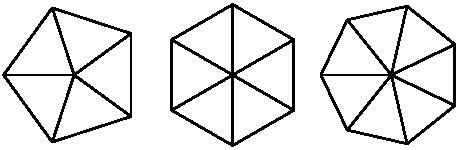
\includegraphics[scale=0.8]{figs/pies.pdf}}
\caption{พายของ Turtle (Turtle pies)}
\label{fig.pies}
\end{figure}


\begin{exercise}
\index{pie}
\index{พาย}

ให้เขียนชุดของฟังก์ชันให้ครอบคลุมการวาดรูปทรงในรูปที่~\ref{fig.pies}

เฉลย: \url{http://thinkpython2.com/code/pie.py}.

\end{exercise}

\begin{exercise}
\index{alphabet}
\index{turtle typewriter}
\index{typewriter, turtle}
\index{พยัญชนะ}
\index{เครื่องพิมพ์ turtle}
\index{เครื่องพิมพ์, turtle}

ตัวอักษรของพยัญชนะสามารถสร้างได้จากส่วนประกอบเล็ก ๆ เช่น เส้นตั้ง เส้นนอน และเส้นโค้งจำนวนไม่กี่เส้น
ให้ออกแบบพยัญชนะที่สามารถวาดจากส่วนประกอบเล็ก ๆ เหล่านี้ในจำนวนที่น้อยที่สุด
จากนั้นให้เขียนฟังก์ชันที่วาดอักษรเหล่านี้

เราควรจะเขียนหนึ่งฟังก์ชันสำหรับอักษรแต่ละตัว แล้วตั้งชื่อ เช่น \verb"draw_a", \verb"draw_b", และอื่น ๆ
และให้ใส่ฟังก์ชันเหล่านี้ลงในไฟล์ชื่อ {\tt letters.py} เราสามารถดาวน์โหลด ``โปรแกรมพิมพ์ดีด turtle 
(turtle typewriter)''  จาก \url{http://thinkpython2.com/code/typewriter.py} เพื่อที่จะทดสอบ
โค้ดของเรา

เราสามารถดูเฉลยได้จาก \url{http://thinkpython2.com/code/letters.py};
มันต้องกาหรไฟล์นี้ในการรัน
\url{http://thinkpython2.com/code/polygon.py}.

\end{exercise}

\begin{exercise}

อ่านเกี่ยวกับเกลียว (spiral) ได้ที่ \url{http://en.wikipedia.org/wiki/Spiral}; 
จากนั้นเขียนโปรแกรมที่วาดรูปเกลียว Archimedian (หรือเกลียวแบบอื่น ๆ) 
เฉลยอยู่ที่ \url{http://thinkpython2.com/code/spiral.py}
\index{spiral}
\index{Archimedian spiral} 
\index{เกลียว}
\index{เกลียว Archimedian}

\end{exercise}



\chapter{เงื่อนไขและการเรียกซ้ำ }% (Conditionals and recursion)}

หัวข้อหลักของบทนี้ คือ คำสั่ง {\tt if} ซึ่งดำเนินการกับโค้ดต่างกันขึ้นอยู่กับสถานะของโปรแกรม
แต่ก่อนอื่น ผมอยากจะแนะนำตัวดำเนินการใหม่สองตัว: การหารปัดเศษลง (floor division) และโมดูลัส (modulus)


\section{การหารปัดเศษลง % (floor division) 
และโมดูลัส} % (modulus)}

เครื่องหมาย {\bf การหารปัดเศษลง (floor division)}, \verb"//", หารเลขสองตัวแล้วปัดเศษลงให้เป็นเลขจำนวนเต็ม
ตัวอย่างเช่น สมมติว่าเวลาฉายหนัง คือ 105 นาที เราอาจจะอยากทราบว่ามันนานกี่ชั่วโมง การหารแบบปกตินิยมจะให้ค่าเป็นเลขจุดลอย:

\begin{verbatim}
>>> minutes = 105
>>> minutes / 60
1.75
\end{verbatim}

แต่โดยปกติแล้วเราไม่เขียนเลขชั่วโมงแบบมีจุดทศนิยม การหารปัดเศษลงจะให้ค่าจำนวนเต็มของเลขชั่วโมง โดยปัดเศษลง:

\begin{verbatim}
>>> minutes = 105
>>> hours = minutes // 60
>>> hours
1
\end{verbatim}

ในการหาเศษของชั่วโมง เราสามารถลบจำนวนนาทีในหนึ่งชั่วโมงออก:

\begin{verbatim}
>>> remainder = minutes - hours * 60
>>> remainder
45
\end{verbatim}

\index{floor division}
\index{floating-point division}
\index{division!floor}
\index{division!floating-point}
\index{modulus operator}
\index{operator!modulus}
\index{การหารปัดเศษลง}
\index{การหารแบบจุดลอย}
\index{การหาร!ปัดเศษลง}
\index{การหาร!จุดลอย}
\index{ตัวดำเนินการมอดูลัส}
\index{ตัวดำเนินการ!มอดูลัส}

อีกทางหนึ่ง คือ การใช้ {\bf ตัวดำเนินการมอดูลัส (modulus operator)}, \verb"%", ซึ่งจะหารเลขสองตัว
และให้ค่าเป็นเศษของการหาร

\begin{verbatim}
>>> remainder = minutes % 60
>>> remainder
45
\end{verbatim}
%
ตัวดำเนินการมอดูลัสนั้นมีประโยชน์มากกว่าที่คิด เช่น เราสามารถตรวจสอบได้ว่าเลขตัวหนึ่งถูกหารลงตัวจากเลขอีกตัว
ได้หรือไม่---ถ้า {\tt x \% y} เป็นศูนย์ แล้ว {\tt x} จะถูกหารด้วย {\tt y} ลงตัว
\index{divisibility}
\index{การหารลงตัว}

นอกจากนี้ เราสามารถดึงตัวเลขหลักทางขวาสุดออกมาได้ด้วย (หลักเดียวหรือหลายหลัก) เช่น {\tt x \% 10} 
จะได้เลขตัวขวาสุด (หลักหน่วย) ของ {\tt x} (ในฐาน 10) เช่นเดียวกันกับ {\tt x \% 100} จะให้เลขสองหลัก
สุดท้ายออกมา

แต่ถ้าเราใช้ไพธอน 2 การหารเลขจะต่างออกไป ตัวดำเนินการหาร, \verb"/", จะทำการหารแบบปัดเศษถ้าเลขทั้งสอง
เป็นจำนวนเต็ม และจะทำการหารแบบจุดลอยหากเลขตัวใดตัวหนึ่งเป็น {\tt float}
\index{Python 2}
\index{ไพธอน 2}



\section{นิพจน์บูลีน} % (Boolean expressions)}
\index{boolean expression}
\index{expression!boolean}
\index{logical operator}
\index{operator!logical}
\index{นิพจน์บูลีน}
\index{นิพจน์!บูลีน}
\index{ตัวดำเนินการทางตรรกะ}
\index{ตัวดำเนินการ!ตรรกะ}

{\bf นิพจน์บูลีน (boolean expression)} คือนิพจน์ที่มีค่าความจริงเป็น จริง หรือ เท็จ ตัวอย่างต่อไปนี้ใช้ตัวดำเนินการ 
{\tt ==} ซึ่งเปรียบเทียบตัวถูกดำเนินการสองตัว และให้ค่าเป็น จริง {\tt (True)} ถ้าสองค่านั้นเท่ากัน และให้ค่าเป็น
เท็จ {\tt (False)} หากไม่เท่ากัน:  

\begin{verbatim}
>>> 5 == 5
True
>>> 5 == 6
False
\end{verbatim}
%
{\tt True} และ {\tt False} เป็นค่าพิเศษที่มีชนิดเป็น บูล {\tt (bool)}; มันไม่ใช่สายอักขระ:
\index{True special value}
\index{False special value}
\index{special value!True}
\index{special value!False}
\index{bool type}
\index{type!bool}
\index{ค่าพิเศษ True}
\index{ค่าพิเศษ False}
\index{ค่าพิเศษ!True}
\index{ค่าพิเศษ!False}
\index{ชนิด bool}
\index{ชนิด!bool}

\begin{verbatim}
>>> type(True)
<class 'bool'>
>>> type(False)
<class 'bool'>
\end{verbatim}
%
ตัวดำเนินการ {\tt ==} เป็นหนึ่งใน {\bf ตัวดำเนินการเชิงสัมพันธ์ (relational operators)}; ตัวอื่น ๆ คือ:

\begin{verbatim}
      x != y               # x is not equal to y
      x > y                # x is greater than y
      x < y                # x is less than y
      x >= y               # x is greater than or equal to y
      x <= y               # x is less than or equal to y
\end{verbatim}
%
ถึงแม้ว่าเราน่าจะคุ้นเคยกับการดำเนินการเหล่านี้ สัญลักษณ์ที่ใช้ในไพธอนจะต่างกับสัญลักษณ์ที่ใช้ในคณิตศาสตร์
ข้อผิดพลาดที่เกิดขึ้นบ่อยคือการใช้เครื่องหมายเท่ากับ ({\tt =}) แทนที่จะใช้เครื่องหมายเท่ากับคู่ ({\tt ==})
ให้จำไว้ว่า {\tt =} เป็นตัวดำเนินการสำหรับการกำหนดค่า และ {\tt ==} เป็นตัวดำเนินการเชิงสัมพันธ์
ไม่มีการใช้เครื่องหมาย {\tt =<} หรือ {\tt =>}
\index{ตัวดำเนินการเชิงสัมพันธ์}
\index{ตัวดำเนินการ!เชิงสัมพันธ์}
\index{relational operator}
\index{operator!relational}


\section {ตัวดำเนินการทางตรรกะ} % (Logical operators)}
\index{logical operator}
\index{operator!logical}
\index{ตัวดำเนินการทางตรรกะ}
\index{ตัวดำเนินการ!ตรรกะ}

{\bf ตัวดำเนินการทางตรรกะ (logical operators)} มี 3 ตัว:  {\tt and}, {\tt or}, 
และ {\tt not}. ความหมายของตัวดำเนินการเหล่านี้ตรงกับความหมายในภาษาอังกฤษเลย เช่น 
{\tt x > 0 and x < 10} จะเป็นจริงถ้า {\tt x} มากกว่า 0 {\em และ} น้อยกว่า 10 เท่านั้น
\index{and operator}
\index{or operator}
\index{not operator}
\index{operator!and}
\index{operator!or}
\index{operator!not}
\index{ตัวดำเนินการ and}
\index{ตัวดำเนินการ or}
\index{ตัวดำเนินการ not}
\index{ตัวดำเนินการ!and}
\index{ตัวดำเนินการ!or}
\index{ตัวดำเนินการ!not}

{\tt n\%2 == 0 or n\%3 == 0} เป็นจริงถ้า {\em ตัวใดตัวหนึ่ง หรือ ทั้งสองตัว} ของเงื่อนไขเป็นจริง 
นั่นคือ ถ้าเลขนั้นสามารถหารด้วย 2 {\em หรือ} 3 ลงตัว

สุดท้ายนี้ ตัวดำเนินการ {\tt not} จะทำนิพจน์บูลีนให้เป็นนิเสธ (การกลับค่าความจริง) ดังนั้น  
{\tt not (x > y)} จะเป็นจริง ถ้า {\tt x > y} เป็นเท็จ  นั่นคือ ถ้า {\tt x} น้อยกว่าหรือเท่ากับ {\tt y}

จริง ๆ แล้ว ตัวถูกดำเนินการของตัวดำเนินการทางตรรกะควรจะเป็นนิพจน์บูลีน แต่ไพธอนนั้นไม่ค่อยเคร่งครัดเท่าไร
เลขที่ไม่เท่ากับศูนย์ใด ๆ จะถูกแปลให้มีค่าเป็น จริง {\tt True}:

\begin{verbatim}
>>> 42 and True
True
\end{verbatim}
%
ความยืดหยุ่นนี้สามารถเป็นประโยชน์ได้ แต่ก็มีรายละเอียดปลีกย่อยที่จะทำให้สับสนได้ 
เราควรจะหลีกเลี่ยงการทำอะไรแบบนี้ (ยกเว้นว่า เรารู้ตัวว่ากำลังทำอะไรอยู่)


\section{การดำเนินการตามเงื่อนไข} % (Conditional execution)}
\label{conditional.execution}

\index{conditional statement}
\index{statement!conditional}
\index{if statement}
\index{statement!if}
\index{conditional execution}
\index{คำสั่งเงื่อนไข}
\index{คำสั่ง!เงื่อนไข}
\index{คำสั่ง if}
\index{คำสั่ง!if}
\index{การดำเนินการตามเงื่อนไข}

ในการที่จะเขียนโปรแกรมที่เป็นประโยชน์ เราต้องการความสามารถในการตรวจสอบเงื่อนไขเกือบจะตลอดเวลา
และสามารถเปลี่ยนพฤติกรรมของโปรแกรมตามเงื่อนไขนั้น {\bf คำสั่งเงื่อนไข (Conditional statements)} 
มอบความสามารถนี้ให้เรา รูปแบบที่ง่ายที่สุด คือ คำสั่ง {\tt if}:

\begin{verbatim}
if x > 0:
    print('x is positive')
\end{verbatim}
%
นิพจน์บูลีนที่อยู่หลังจาก {\tt if} เรียกว่า {\bf เงื่อนไข (condition)}
ถ้าเงื่อนไขเป็นจริง คำสั่งที่ย่อหน้าเข้าไปนั้นจะถูกรัน ไม่เช่นนั้น ก็ไม่มีอะไรเกิดขึ้น
\index{condition}
\index{compound statement}
\index{statement!compound}
\index{เงื่อนไข}
\index{คำสั่งประกอบ}
\index{คำสั่ง!ประกอบ}

คำสั่ง {\tt if} มีโครงสร้างเหมือนนิยามของฟังก์ชัน: มีส่วนหัว ตามด้วยส่วนตัวที่ถูกย่อหน้าเข้าไป
คำสั่งแบบนี้เรียกว่า {\bf คำสั่งประกอบ (compound statements)}

มันไม่มีข้อจำกัดสำหรับจำนวนคำสั่งที่ปรากฏในส่วนตัวของคำสั่ง if แต่จะต้องมีอย่างน้อยหนึ่งคำสั่ง
ในบางครั้ง มันก็มีประโยชน์ที่จะมีส่วนตัวที่ไม่มีคำสั่ง (โดยปกติแล้วใช้เป็นที่สำรองสำหรับโค้ดที่ยังไม่ได้เขียน)
ในกรณีดังกล่าว เราสามารถใส่คำสั่ง {\tt pass} ซึ่งเป็นคำสั่งที่ไม่ทำอะไรเลย 
\index{pass statement}
\index{statement!pass}
\index{คำสั่ง pass}
\index{คำสั่ง!pass}

\begin{verbatim}
if x < 0:
    pass          # TODO: need to handle negative values!
\end{verbatim}
%


\section{การดำเนินการทางเลือก} % (Alternative execution)}
\label{alternative.execution}
\index{alternative execution}
\index{else keyword}
\index{keyword!else}
\index{การดำเนินการทางเลือก}
\index{คำสำคัญ else}
\index{คำสำคัญ!else}

ีรูปแบบที่สองของคำสั่ง {\tt if} คือ ``การดำเนินการทางเลือก (alternative execution)''
ซึ่งมีทางเลือกทำสองทางและมีเงื่อนไขที่จะกำหนดว่าคำสั่งชุดไหนจะถูกรัน กฎวากยสัมพันธ์ของคำสั่งเป็นแบบนี้:

\begin{verbatim}
if x % 2 == 0:
    print('x is even')
else:
    print('x is odd')
\end{verbatim}
%
ถ้าเศษของการหารเมื่อเราหาร {\tt x} ด้วย 2 มีค่าเป็น 0 แล้ว เรารู้ว่า {\tt x} เป็นจำนวนคู่
และโปรแกรมจะแสดงข้อความตามนั้น  แต่ถ้าเงื่อนไขเป็นเท็จ คำสั่งชุดที่สองจะทำงาน
เนื่องจากเงื่อนไขจะต้องเป็นจริงหรือเท็จเท่านั้น จึงมีแค่ทางเลือกหนึ่งอย่างเท่านั้นที่ทำงาน
ทางเลือกเหล่านี้เรียกว่า {\bf (แขนง) branches} เพราะว่ามันเป็นกิ่งที่แตกแยกออกไป
ของกระแสการดำเนินการ (flow of execution)
\index{branch}
\index{แขนง}



\section{เงื่อนไขลูกโซ่} % (Chained conditionals)}
\index{chained conditional}
\index{conditional!chained}
\index{เงื่อนไขลูกโซ่}
\index{เงื่อนไข!ลูกโซ่}

บางครั้งมันก็มีมากกว่าสองทางเลือก และเราต้องการมากกว่าสองแขนงที่แตกออกไป ทางหนึ่งในการแสดง
การคำนวณแบบนี้ คือ {\bf เงื่อนไขลูกโซ่ (chained conditional)}

\begin{verbatim}
if x < y:
    print('x is less than y')
elif x > y:
    print('x is greater than y')
else:
    print('x and y are equal')
\end{verbatim}
%
{\tt elif} เป็นคำย่อของ ``else if'' (ไม่เช่นนั้น ถ้า) ทบทวนอีกทีว่าแขนงแค่หนึ่งอันเท่านั้นที่จะทำงาน
มันไม่มีการจำกัดจำนวนของคำสั่ง {\tt elif}  ถ้าจะมีข้อย่อย (clause) {\tt else} ด้วย 
มันจะต้องอยู่ท้ายสุด แต่มันไม่จำเป็นต้องมี
\index{elif keyword}
\index{keyword!elif}
\index{คำสำคัญ elif}
\index{คำสำคัญ!elif}

\begin{verbatim}
if choice == 'a':
    draw_a()
elif choice == 'b':
    draw_b()
elif choice == 'c':
    draw_c()
\end{verbatim}
%
เงื่อนไขแต่ละอันจะถูกตรวจสอบตามลำดับ ถ้าอันแรกเป็นเท็จ อันถัดไปจะถูกตรวจสอบ และเป็นแบบนี้ไปเรื่อย ๆ
ถ้าเงื่อนไขใดเป็นจริง คำสั่งในแขนงนั้นจะทำงาน และชุดคำสั่งนี้จะจบการทำงาน
แม้ว่ามีเงื่อนไขมากกว่าหนึ่งที่เป็นจริง แต่แค่คำสั่งในแขนงของเงื่อนไขแรกที่เป็นจริงเท่านั้นที่จะทำงาน


\section{เงื่อนไขซ้อนใน} % (Nested conditionals)}
\index{nested conditional}
\index{conditional!nested}
\index{เงื่อนไขซ้อนใน}
\index{เงื่อนไข!ซ้อนใน}

เงื่อนไขหนึ่ง ๆ สามารถซ้อนในเงื่อนไขอื่นได้ เราสามารถเขียนตัวอย่างในหัวข้อที่แล้วให้เป็นแบบนี้ได้:

\begin{verbatim}
if x == y:
    print('x and y are equal')
else:
    if x < y:
        print('x is less than y')
    else:
        print('x is greater than y')
\end{verbatim}
%
เงื่อนไขด้านนอกมีสองแขนง แขนงแรกมีคำสั่งง่าย ๆ คำสั่งเดียว
แขนงที่สองมีคำสั่ง {\tt if} อีกอันบรรจุอยู่ ซึ่งก็มีเงื่อนไขอีกสองแขนงย่อยลงไปอีก 
ทั้งสองแขนงข้างในนั้นมีคำสั่งแบบง่าย ๆ อยู่ แม้ว่าข้างในสามารถเป็นเงื่อนไขอีกชั้นหนึ่งก็ได้

แม้ว่าการย่อหน้าของคำสั่งต่าง ๆ ทำให้โปรแกรมมีโครงสร้างที่ชัดเจน  แต่ {\bf เงื่อนไขซ้อนใน 
(nested conditionals)} มันทำให้อ่านยากเวลาอ่านเร็ว ๆ จึงเป็นความคิดที่ดีที่จะหลีกเลี่ยงถ้าทำได้

ตัวดำเนินการทางตรรกะสามารถทำให้เราเขียนคำสั่งเงื่อนไขซ้อนในให้ง่ายขึ้น เช่น เราสามารถเขียน
โค้ดต่อไปนี้อีกแบบหนึ่ง โดยใช้เงื่อนไขแบบเดี่ยว:

\begin{verbatim}
if 0 < x:
    if x < 10:
        print('x is a positive single-digit number.')
\end{verbatim}
%
คำสั่ง {\tt print} จะทำงานถ้าเราผ่านเงื่อนไขทั้งสองนี้ได้ ดังนั้น เราสามารถทำให้เกิดผลอย่างเดียวกัน 
โดยการใช้ตัวดำเนินการ {\tt and}:

\begin{verbatim}
if 0 < x and x < 10:
    print('x is a positive single-digit number.')
\end{verbatim}

สำหรับเงื่อนไขประเภทนี้ ไพธอนมีทางเลือกให้ทำแบบกระชับ:

\begin{verbatim}
if 0 < x < 10:
    print('x is a positive single-digit number.')
\end{verbatim}


\section{การเรียกซ้ำ} % (Recursion)}
\label{recursion}
\index{recursion}
\index{การเรียกซ้ำ}


ฟังก์ชันหนึ่ง ๆ สามารถเรียกฟังก์ชันอื่นได้; ฟังก์ชันหนึ่ง ๆ ยังสามารถเรียกตัวเองได้ด้วย
มันอาจจะไม่ชัดเจนว่าทำไมมันเป็นสิ่งที่ดี แต่ปรากฎว่ามันเป็นสิ่งมหัศจรรย์อย่างหนึ่งเลย
ที่โปรแกรมสามารถทำได้ เช่น ให้ดูฟังก์ชันต่อไปนี้:

\begin{verbatim}
def countdown(n):
    if n <= 0:
        print('Blastoff!')
    else:
        print(n)
        countdown(n-1)
\end{verbatim}
%
ถ้า {\tt n} เป็น 0 หรือมีค่าลบ มันจะแสดงคำว่า ``Blastoff!'' ออกมา
ไม่เช่นนั้น มันจะแสดงค่า {\tt n} ออกมาและเรียกฟังก์ชันที่ชื่อว่า {\tt countdown}---ตัวมันเอง---โดยผ่านค่า {\tt n-1} เป็นอาร์กิวเมนต์

จะเกิดอะไรขึ้นถ้าเราเรียกฟังก์ชันนี้ในลักษณะนี้?

\begin{verbatim}
>>> countdown(3)
\end{verbatim}
%
การดำเนินการของฟังก์ชัน {\tt countdown} เริ่มด้วย {\tt n=3} และเนื่องจาก {\tt n} มีค่ามากกว่า 0
ฟังก์ชันจะแสดงค่า 3 ออกมาและจากนั้นจึงเรียกตัวมันเอง...


\begin{quote}
การทำงานของฟังก์ชัน {\tt countdown} เริ่มด้วย {\tt n=2} และเนื่องจาก {\tt n} มีค่ามากกว่า 0
ฟังก์ชันจะแสดงค่า 2 ออกมาและจากนั้นจึงเรียกตัวมันเอง...

\begin{quote}
การทำงานของฟังก์ชัน {\tt countdown} เริ่มด้วย {\tt n=1} และเนื่องจาก {\tt n} มีค่ามากกว่า 0
ฟังก์ชันจะแสดงค่า 1 ออกมาและจากนั้นจึงเรียกตัวมันเอง...

\begin{quote}
การทำงานของฟังก์ชัน {\tt countdown} เริ่มด้วย {\tt n=0} และเนื่องจาก {\tt n} มีค่าไม่มากกว่า 0
ฟังก์ชันจะแสดงคำว่า ``Blastoff!'' ออกมา จบ และกลับออกไป
\end{quote}

ฟังก์ชัน {\tt countdown} ที่ได้รับค่า {\tt n=1} มาก็จบ และกลับออกไป
\end{quote}

ฟังก์ชัน {\tt countdown} ที่ได้รับค่า {\tt n=2} มาก็จบ และกลับออกไป
\end{quote}

ฟังก์ชัน {\tt countdown} ที่ได้รับค่า {\tt n=3} มาก็จบ และกลับออกไป

และจากนั้นเราก็กลับมายัง \verb"__main__"  ดังนั้น เอ้าต์พุตทั้งหมดจะหน้าตาเป็นแบบนี้:
\index{main}

\begin{verbatim}
3
2
1
Blastoff!
\end{verbatim}
% 
ฟังก์ชันที่เรียกตัวมันเอง คือ ฟังก์ชัน {\bf เรียกซ้ำ (recursive)} หรือ ฟังก์ชันเวียนเกิด (ในหนังสือเล่มนี้
จะเรียกว่า ฟังก์ชันเรียกซ้ำ); กระบวนการทำงานของมันเรียกว่า การเรียกซ้ำ {\bf recursion}
\index{recursion}
\index{function!recursive}
\index{การเรียกซ้ำ}
\index{ฟังก์ชัน!เวียนเกิด}
\index{ฟังก์ชัน!เรียกซ้ำ}

อีกตัวอย่างหนึ่ง เราสามารถเขียนฟังก์ชันที่พิมพ์สายอักขระจำนวน {\tt n} ครั้ง

\begin{verbatim}
def print_n(s, n):
    if n <= 0:
        return
    print(s)
    print_n(s, n-1)
\end{verbatim}
%
ถ้า {\tt n <= 0} คำสั่ง {\bf return} จะทำให้จบฟังก์ชัน กระแสการดำเนินการจะกลับไปยังตัวเรียก (caller) ทันที
และบรรทัดที่เหลือในฟังก์ชันนั้นจะไม่ถูกรัน
\index{return statement}
\index{statement!return}
\index{คำสั่ง return}
\index{คำสั่ง!return}

ส่วนที่เหลือของฟังก์ชันนั้นเหมือนกับฟังก์ชัน {\tt countdown}: มันแสดง {\tt s} และจากนั้นเรียกตัวเองเพื่อแสดง {\tt s} ไปอีก $n-1$ ครั้ง
ดังนั้น จำนวนบรรทัดของเอ้าต์พุตจะเป็น {\tt 1 + (n - 1)} ซึ่งรวมกันแล้วได้ {\tt n} บรรทัด

สำหรับตัวอย่างง่าย ๆ แบบนี้ มันอาจจะง่ายกว่าที่จะใช้ลูป {\tt for} แต่เราจะเห็นตัวอย่างอีกมากในภายหลังที่ยากที่จะเขียนด้วย ลูป {\tt for}
และง่ายที่จะเขียนด้วยการเรียกซ้ำ (recursion)  ดังนั้น จึงเป็นเรื่องที่ดีที่จะเริ่มเข้าใจหัวข้อนี้ก่อน
\index{for loop}
\index{loop!for}
\index{ลูป for}
\index{ลูป!for}


\section{แผนภาพแบบกองซ้อนสำหรับฟังก์ชันเรียกซ้ำ}% (Stack diagrams for recursive functions)}
\label{recursive.stack}
\index{stack diagram}
\index{function frame}
\index{frame}
\index{แผนภาพแบบกองซ้อน}
\index{กรอบฟังก์ชัน}
\index{กรอบ}

ในหัวข้อที่~\ref{stackdiagram} เราใช้แผนภาพแบบกองซ้อนในการแสดงสถานะของโปรแกรม
ในขณะที่มีการเรียกฟังก์ชัน แผนภาพชนิดเดียวกันนี้สามารถช่วยให้เข้าใจฟังก์ชันเรียกซ้ำ (recursive function) ได้ด้วย

ทุกครั้งที่ฟังก์ชันถูกเรียก ไพธอนจะสร้างกรอบที่บรรจุตัวแปรเฉพาะที่และพารามิเตอร์ของฟังก์ชัน
สำหรับฟังก์ชันเรียกซ้ำ มันอาจจะมีกรอบมากกว่าหนึ่งกรอบบนกอง ณ ขณะหนึ่ง

รูปที่~\ref{fig.stack2} แสดงแผนภาพแบบกองซ้อนสำหรับฟังก์ชัน {\tt countdown} ที่ถูกเรียกด้วยค่า {\tt n = 3}.

\begin{figure}
\centerline
{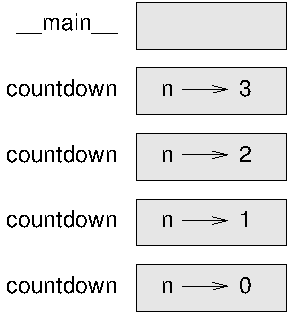
\includegraphics[scale=0.8]{figs/stack2.pdf}}
\caption{แผนภาพแบบกองซ้อน (Stack diagram)}
\label{fig.stack2}
\end{figure}


เหมือนทั่วไป บนสุดของกองคือกรอบของ \verb"__main__" มันว่างเปล่าเพราะว่าเราไม่ได้สร้างตัวแปรใด ๆ ใน \verb"__main__"
หรือไม่ได้ผ่านอาร์กิวเมนต์ใด ๆ เข้าไป
\index{base case}
\index{recursion!base case}
\index{กรณีฐาน}
\index{การเรียกซ้ำ!กรณีฐาน}

กรอบ {\tt countdown} ทั้ง 4 กรอบ มีค่าพารามิเตอร์ {\tt n} ที่ต่างกัน
ล่างสุดของกองซึ่ง {\tt n=0} เรียกว่า {\bf กรณีฐาน (base case)} มันไม่ได้เรียกตัวเองซ้ำ 
ดังนั้น จึงไม่มีกรอบเพิ่มไปอีก


เพื่อเป็นการฝึกทำ ให้วาดแผนภาพแบบกองซ้อนสำหรับฟังก์ชัน \verb|print_n| ที่ถูกเรียกด้วยค่า 
\verb"s = 'Hello'" และ {\tt n=2} จากนั้นให้เขียนฟังก์ชันชื่อว่า \verb"do_n" 
ที่รับวัตถุฟังก์ชันและจำนวน {\tt n} เข้าเป็นอาร์กิวเมนต์ และมันจะเรียกฟังก์ชันที่กำหนดให้เป็นจำนวน {\tt n} ครั้ง



\section{การเรียกซ้ำไม่รู้จบ} % (Infinite recursion)}
\index{infinite recursion}
\index{recursion!infinite}
\index{runtime error}
\index{error!runtime}
\index{traceback}
\index{การเรียกซ้ำไม่รู้จบ}
\index{การเรียกซ้ำ!ไม่รู้จบ}
\index{ข้อผิดพลาดตอนโปรแกรมทำงาน}
\index{ข้อผิดพลาด!ตอนโปรแกรมทำงาน}
\index{การย้อนรอย}

ถ้าการเรียกซ้ำไม่ไปถึงกรณีฐาน (base case) เสียที มันจะทำให้เกิดการเรียกซ้ำไปตลอดกาล
และโปรแกรมก็จะไม่จบ นี่เรียกว่า {\bf การเรียกซ้ำไม่รู้จบ (infinite recursion)}
และมันก็ไม่ได้เป็นความคิดที่ดีเท่าไรนัก นี่คือ โปรแกรมแบบสั้นที่สุดที่จะทำให้เกิดการเรียกซ้ำแบบไม่สิ้นสุด:

\begin{verbatim}
def recurse():
    recurse()
\end{verbatim}
%
ในสภาพแวดล้อมของการเขียนโปรแกรมส่วนใหญ่ โปรแกรมจะไม่ทำงานไปตลอดกาลแบบนั้น
ไพธอนจะรายงานข้อความความผิดพลาดเมื่อมีการเรียกซ้ำจนถึงความลึกที่มากที่สุด (ที่อนุญาตให้รันได้):
\index{exception!RuntimeError}
\index{RuntimeError}
\index{ข้อยกเว้น!ข้อผิดพลาดตอนโปรแกรมทำงาน}
\index{ข้อผิดพลาดตอนโปรแกรมทำงาน}

\begin{verbatim}
  File "<stdin>", line 2, in recurse
  File "<stdin>", line 2, in recurse
  File "<stdin>", line 2, in recurse
                  .   
                  .
                  .
  File "<stdin>", line 2, in recurse
RuntimeError: Maximum recursion depth exceeded
\end{verbatim}
%
การย้อนรอยแบบนี้มันจะเยอะกว่าที่เราเคยทำในบทก่อนหน้านี้นิดหน่อย 
เมื่อเกิดข้อผิดพลาดในตัวอย่างนี้ขึ้นมา มันมี 1000 {\tt recurse} frames (กรอบการเรียกซ้ำ) บนกองนี้!

ถ้าเราเจอการเรียกซ้ำไม่รู้จบโดยบังเอิญ ให้ทบทวนฟังก์ชันของเราเพื่อให้แน่ใจว่ามันมีกรณีฐาน 
(base case) ที่ไม่เรียกตัวเองซ้ำ และถ้ามีกรณีฐานแล้ว ให้ตรวจสอบว่าเราจะไปถึงมันจริง ๆ


\section{การนำเข้าข้อมูลผ่านคีย์บอร์ด}% (Keyboard input)}
\index{keyboard input}
\index{การนำเข้าข้อมูลผ่านคีย์บอร์ด}

โปรแกรมที่เราเขียนมาถึงตอนนี้ไม่ได้รับอินพุต (input) มาจากผู้ใช้
มันแค่ทำอะไรซ้ำ ๆ ตลอดเวลา

ไพธอนได้เตรียมฟังก์ชันพร้อมใช้เรียกว่า {\tt input} ที่หยุดโปรแกรมและรอให้ผู้ใช้พิมพ์อะไรสักอย่างเข้ามา
เมื่อผู้ใช้กดปุ่ม {\sf Return} หรือ {\sf Enter} โปรแกรมจะทำงานต่อ และฟังก์ชัน \verb"input" จะคืนค่า
สิ่งที่ผู้ใช้พิมพ์เข้ามาเป็นชนิดสายอักขระ  ในไพธอน 2 ฟังก์ชันที่ทำงานแบบเดียวกันนี้เรียกว่า \verb"raw_input"
\index{Python 2}
\index{input function}
\index{function!input}
\index{ไพธอน 2}
\index{ฟังก์ชันนำข้อมูลเข้า}
\index{ฟังก์ชัน!ข้อมูลนำเข้า}

\begin{verbatim}
>>> text = input()
What are you waiting for?
>>> text
'What are you waiting for?'
\end{verbatim}
%
ก่อนที่จะรับอินพุตมาจากผู้ใช้ มันเป็นความคิดที่ดีที่จะพิมพ์ข้อความไปบอกผู้ใช้ว่าให้พิมพ์อะไรเข้ามา 
ฟังก์ชัน \verb"input" สามารถรับข้อความพร้อมรับ (prompt) เป็นอาร์กิวเมนต์ได้:
\index{prompt}
\index{ข้อความพร้อมรับ}

\begin{verbatim}
>>> name = input('What...is your name?\n')
What...is your name?
Arthur, King of the Britons!
>>> name
'Arthur, King of the Britons!'
\end{verbatim}
%
ลำดับอักขระ \verb"\n" ในตอนท้ายของข้อความพร้อมรับเป็นตัวแทนของ {\bf บรรทัดใหม่ (newline)}
ซึ่งเป็นอักขระพิเศษที่ทำให้เกิดการขึ้นบรรทัดใหม่ นั่นคือเหตุผลที่อินพุตของผู้ใช้ปรากฏอยู่ข้างใต้ข้อความพร้อมรับ
\index{newline}
\index{บรรทัดใหม่}

ถ้าเราคาดหวังว่าผู้ใช้จะพิมพ์จำนวนเต็มเข้ามา เราสามารถลองแปลงค่าที่คืนกลับมาเป็น {\tt int}:

\begin{verbatim}
>>> prompt = 'What...is the airspeed velocity of an unladen swallow?\n'
>>> speed = input(prompt)
What...is the airspeed velocity of an unladen swallow?
42
>>> int(speed)
42
\end{verbatim}
%
แต่ถ้าผู้ใช้พิมพ์อย่างอื่นที่ไม่ใช่สายอักขระของตัวเลขแล้วล่ะก็ เราก็จะได้ข้อผิดพลาด:

(หมายเหตุผู้แปล: ได้ข้อผิดพลาดตอนที่พยายามแปลงให้เป็น int)

\begin{verbatim}
>>> speed = input(prompt)
What...is the airspeed velocity of an unladen swallow?
What do you mean, an African or a European swallow?
>>> int(speed)
ValueError: invalid literal for int() with base 10
\end{verbatim}
%
เราจะรู้ว่าจะจัดการกับข้อผิดพลาดประเภทนี้อย่างไรในภายหลัง
\index{ValueError}
\index{exception!ValueError}
\index{ข้อผิดพลาดของค่า}
\index{ข้อยกเว้น!ข้อผิดพลาดของค่า}


\section{การดีบัก}
\label{whitespace}
\index{debugging}
\index{traceback}
\index{การดีบัก}
\index{การย้อนรอย}

% When a syntax or runtime error occurs, the error message contains
% a lot of information, but it can be overwhelming.  The most
% useful parts are usually:
เมื่อเกิดข้อผิดพลาดเชิงวากยสัมพันธ์ (syntax error) หรือข้อผิดพลาดตอนดำเนินการ (runtime error)
ข้อความแจ้งข้อผิดพลาด (error message) มีข้อมูลจำนวนมากให้เรา แต่มันจะทำให้เรารู้สึกท้วมท้นมาก 
ส่วนที่เป็นประโยชน์โดยปกติแล้วจะเป็น:

\begin{itemize}

\item ข้อผิดพลาดที่เกิดขึ้นเป็นชนิดใด และ

\item มันเกิดขึ้นที่ไหน

\end{itemize}

ข้อผิดพลาดเชิงวากยสัมพันธ์นั้นง่ายที่จะหา แต่มันก็มีข้อต้องระวังนิดหน่อย 
ข้อผิดพลาดที่เกี่ยวกับการเว้นวรรค (whitespace error) อาจจะทำให้เราปวดหัวได้ 
เพราะว่าช่องว่างและย่อหน้านั้นมันมองไม่เห็น และเราก็ชินกับการไม่สนใจมัน
\index{whitespace}
\index{เว้นวรรค}

\begin{verbatim}
>>> x = 5
>>>  y = 6
  File "<stdin>", line 1
    y = 6
    ^
IndentationError: unexpected indent
\end{verbatim}
%
ในตัวอย่างนี้ ปัญหา คือ บรรทัดที่สองนั้นถูกย่อหน้าเข้าไปโดยช่องว่าง 1 ช่อง
แต่ข้อผิดพลาดนั้นชี้ไปที่ตัวแปร y ซึ่งอาจจะทำให้ไขว้เขวได้
โดยทั่วไปแล้ว ข้อความแจ้งข้อผิดพลาดจะระบุตำแหน่งตรงที่เจอปัญหา แต่ข้อผิดพลาดจริง ๆ 
อาจจะอยู่ก่อนตำแหน่งที่ระบุก็ได้ บางทีก็อยู่ในบรรทัดก่อนหน้า 
\index{error!runtime}
\index{runtime error}
\index{ข้อผิดพลาด!ตอนโปรแกรมทำงาน}
\index{ข้อผิดพลาดตอนโปรแกรมทำงาน}

เช่นเดียวกันกับข้อผิดพลาดตอนดำเนินการ สมมติว่าเราพยายามที่จะคำนวณอัตราส่วนระหว่าง
สัญญาณและสัญญาณรบกวน (signal-to-noise ratio) ในหน่วยเดซิเบล สูตรคือ $SNR_{db} = 10 \log_{10} (P_{signal} / P_{noise})$
ในไพธอน เราน่าจะเขียนประมาณนี้:

\begin{verbatim}
import math
signal_power = 9
noise_power = 10
ratio = signal_power // noise_power
decibels = 10 * math.log10(ratio)
print(decibels)
\end{verbatim}
%
เมื่อเรารันโปรแกรม เราจะได้ข้อยกเว้น:
%
\index{exception!OverflowError}
\index{OverflowError}
\index{ข้อยกเว้น!ข้อผิดพลาดแบบข้อมูลเกินเก็บ}
\index{ข้อผิดพลาดแบบข้อมูลเกินเก็บ}

\begin{verbatim}
Traceback (most recent call last):
  File "snr.py", line 5, in ?
    decibels = 10 * math.log10(ratio)
ValueError: math domain error
\end{verbatim}
%
ข้อความแจ้งข้อผิดพลาดระบุว่ามีปัญหาที่บรรทัดที่ 5 แต่ก็ไม่เห็นมีอะไรผิดนี่นา 
เพื่อที่จะหาข้อผิดพลาดที่แท้จริง มันอาจจะเป็นประโยชน์ที่จะพิมพ์ค่าของ {\tt ratio} ออกมาดู 
ซึ่งมีค่าเป็น 0 ปัญหาจึงอยู่ที่บรรทัดที่ 4 ที่ใช้การหารแบบปัดเศษลง แทนที่จะใช้การหารแบบจุดลอย
\index{floor division}
\index{division!floor}
\index{การหารปัดเศษลง}
\index{การหาร!ปัดเศษลง}

เราควรที่จะใช้เวลาในการอ่านข้อความแจ้งข้อผิดพลาดอย่างระมัดระวัง
แต่อย่าคิดเอาเองว่า ทุกสิ่งมันบอกเรานั้นถูกต้องเป๊ะตามนั้น


\section{อภิธานศัพท์}

\begin{description}

\item[การหารปัดเศษลง (floor division):] ตัวดำเนินการที่มีเครื่องหมายเป็น {\tt //} ซึ่งหารเลขสองตัวและปัดเศษลงให้เป็นจำนวนเต็ม
\index{floor division} 
\index{division!floor}
\index{การหารปัดเศษลง}
\index{การหาร!ปัดเศษลง}

\item[ตัวดำเนินการมอดูลัส (modulus operator):]  ตัวดำเนินการที่มีเครื่องหมายเป็นเปอร์เซ็นต์ ({\tt \%})
ซึ่งทำงานกับจำนวนเต็มและคืนค่าเป็นเศษของการหาร 
\index{modulus operator}
\index{operator!modulus}
\index{ตัวดำเนินการมอดูลัส}
\index{ตัวดำเนินการ!มอดูลัส}

\item[นิพจน์บูลีน (boolean expression):] นิพจน์ที่มีค่าเป็น {\tt True} (จริง) หรือ {\tt False} (เท็จ)
\index{boolean expression}
\index{expression!boolean}
\index{นิพจน์บูลีน}
\index{นิพจน์+บูลีน}

\item[ตัวดำเนินการเชิงสัมพันธ์ (relational operator):] ตัวดำเนินการที่เปรียบเทียบค่าของตัวถูกดำเนินการ: 
{\tt ==}, {\tt !=}, {\tt >}, {\tt <}, {\tt >=}, และ {\tt <=}

\item[ตัวดำเนินการเชิงตรรกะ (logical operator):] ตัวดำเนินการที่เชื่อมประกอบนิพจน์บูลีน: 
{\tt and}, {\tt or}, และ {\tt not}

\item[คำสั่งเงื่อนไข (conditional statement):]  คำสั่งที่ควบคุมการทำงานของโปรแกรมให้ขึ้นอยู่กับเงื่อนไขบางอย่าง
\index{conditional statement}
\index{statement!conditional}
\index{คำสั่งเงื่อนไข}
\index{คำสั่ง!เงื่อนไข}

\item[เงื่อนไข (condition):] นิพจน์บูลีนในคำสั่งเงื่อนไขที่กำหนดว่าแขนงไหนของคำสั่งจะถูกทำงาน 
\index{condition}
\index{เงื่อนไข}

\item[คำสั่งประกอบ (compound statement):]  คำสั่งที่ประกอบด้วยส่วนหัว (header) และส่วนตัว (body)
ส่วนหัวจะลงท้ายด้วยเครื่องหมายทวิภาค หรือ โคลอน (:) ส่วนตัวจะถูกย่อหน้าเข้าไปให้สัมพันธ์กับส่วนหัว 
\index{compound statement}
\index{คำสั่งประกอบ}

\item[แขนง (branch):] ชุดคำสั่งที่เป็นทางเลือกอันหนึ่งของคำสั่งเงื่อนไข 
\index{branch}
\index{แขนง}

\item[เงื่อนไขลูกโซ่ (chained conditional):]  คำสั่งเงื่อนไขที่มีชุดของแขนงทางเลือกหลาย ๆ อัน
\index{chained conditional}
\index{conditional!chained}
\index{เงื่อนไขลูกโซ่}
\index{เงื่อนไข!ลูกโซ่}

\item[เงื่อนไขซ้อนใน (nested conditional):]  คำสั่งเงื่อนไขที่ปรากฏอยู่ในแขนงหนึ่งของคำสั่งเงื่อนไขอีกอันหนึ่ง
\index{nested conditional}
\index{conditional!nested}
\index{เงื่อนไขซ้อนใน}
\index{เงื่อนไข!ซ้อนใน}

\item[คำสั่งคืนค่า (return statement):] คำสั่งที่ทำให้ฟังก์ชันจบการทำงานทันทีและคืนการทำงานให้กับตัวเรียก (caller)

\item[การเรียกซ้ำ (recursion):] ขั้นตอนของการเรียกฟังก์ชันตัวที่กำลังรันอยู่ (หมายเหตุผู้แปล: การเรียกตัวมันเอง) 
\index{recursion}
\index{การเรียกซ้ำ}

\item[กรณีฐาน (base case):]  แขนงเงื่อนไขหนึ่งในฟังก์ชันเรียกซ้ำที่ไม่มีการเรียกตัวเองซ้ำ
\index{base case}
\index{กรณีฐาน}

\item[การเรียกซ้ำไม่รู้จบ (infinite recursion):]  การเรียกซ้ำที่ไม่มีกรณีฐาน (base case) หรือไม่มีทางเรียกกรณีฐานเลย
ในที่สุดแล้ว การเรียกซ้ำไม่รู้จบจะทำให้เกิดข้อผิดพลาดในการดำเนินการ (runtime error) 
\index{infinite recursion}
\index{การเรียกซ้ำไม่รู้จบ}

\end{description}

\section{แบบฝึกหัด}

\begin{exercise}

มอดูล {\tt time}  มีฟังก์ชันที่ชื่อว่า {\tt time} ให้ใช้ ซึ่งคืนค่าเป็นเวลามาตรฐานโลกตามนาฬิกาที่กรีนิช 
(Greenwich Mean Time: GMT) ณ ปัจจุบัน อ้างอิงจาก ``the epoch'' ซึ่งเป็นเวลามาตรฐานที่ใช้อ้างอิง 
บนระบบยูนิกซ์  epoch คือ วันที่ 1 มกราคม ค.ศ. 1970

(หมายเหตุผู้แปล: epoch อ่านว่า เอพ'เพิค คือเวลา 00:00:00 UTC ของวันที่ 1 มกราคม ค.ศ. 1970)

\begin{verbatim}
>>> import time
>>> time.time()
1437746094.5735958
\end{verbatim}

ให้เขียนสคริปต์ที่อ่านเวลาปัจจุบัน และแปลงให้เป็นเวลาในหน่วยชั่วโมง นาที และวินาที และจำนวนวันตั้งแต่ the epoch

\end{exercise}


\begin{exercise}
\index{Fermat's Last Theorem}
\index{ทฤษฎีบทสุดท้ายของแฟร์มา}

ทฤษฎีบทสุดท้ายของแฟร์มา (Fermat's Last Theorem) ระบุว่า ไม่มีจำนวนเต็มบวก
$a$, $b$, และ $c$ ใด ๆ ที่ทำให้: 

\[ a^n + b^n = c^n \]
%
สำหรับค่าใด ๆ ของ $n$ ที่มากกว่า 2

\begin{enumerate}

% \item Write a function named \verb"check_fermat" that takes four
% parameters---{\tt a}, {\tt b}, {\tt c} and {\tt n}---and
% checks to see if Fermat's theorem holds.  If
% $n$ is greater than 2 and 
\item ให้เขียนฟังก์ชันที่ชื่อว่า \verb"check_fermat" ซึ่งรับค่าพารามิเตอร์ 4 ค่า
---{\tt a}, {\tt b}, {\tt c} และ {\tt n}--- และตรวจสอบว่าทฤษฎีบทสุดท้ายของแฟร์มา
นั้นจริงหรือไม่ ถ้า $n$ มากกว่า 2 และ

\[a^n + b^n = c^n \]
%
โปรแกรมควรจะพิมพ์ว่า ``Holy smokes, Fermat was wrong!''
ไม่เช่นนั้น โปรแกรมควรจะพิมพ์ว่า ``No, that doesn't work.''

\item ให้เขียนฟังก์ชันที่รับค่า {\tt a}, {\tt b}, {\tt c} และ {\tt n} จากผู้ใช้ แปลงค่าเหล่านี้
เป็นจำนวนเต็ม และใช้ฟังก์ชัน \verb"check_fermat" ตรวจสอบดูว่าค่าเหล่านี้ผ่าฝืนทฤษฎี
บทสุดท้ายของแฟร์มาหรือไม่

\end{enumerate}

\end{exercise}


\begin{exercise}
\index{triangle}
\index{สามเหลี่ยม}

ถ้าเราได้กิ่งไม้มาสามชิ้น เราอาจจะหรืออาจจะไม่สามารถที่จะเรียงมันให้เป็น
สามเหลี่ยมได้ เช่น ถ้าไม้อันหนึ่งยาว 12 นิ้ว และอีกสองอันยาวอันละ 1 นิ้ว เราจะไม่
สามารถทำให้ไม้แท่งสั้นประกบกันได้ สำหรับความยาวของไม้ทั้งสามแท่ง มันมีการทดสอบแบบ
ง่าย ๆ เพื่อที่จะดูว่ามันสามารถที่จะประกอบกันเป็นสามเหลี่ยมได้หรือไม่:

\begin{quotation}
ถ้าความยาวของด้านใดด้านหนึ่งนั้นยาวมากกว่าผลรวมของอีกสองด้านที่เหลือ 
เราจะไม่สามารถสร้างสามเหลี่ยมได้ นอกจากนี้ เราจะสามารถทำได้ (ถ้าผล
รวมของสองด้าน เท่ากับด้านที่สาม มันจะประกอบกันเป็นสิ่งที่เรียกว่า 
สามเหลี่ยมลดรูป หรือ ``degenerate'' triangle)
\end{quotation}

(หมายเหตุผู้แปล: สามเหลี่ยมลดรูป หรือ degenerate triangle คือ สามเหลี่ยมที่ไม่เห็น
เป็นรูปสามเหลี่ยมทั่วไป แต่เป็นคล้าย ๆ เส้นตรงแทน)

\begin{enumerate}

\item ให้เขียนฟังก์ชันชื่อว่า \verb"is_triangle" ซึ่งรับจำนวนเต็มมาเป็นอาร์กิวเมนต์ 
และพิมพ์ ``Yes'' หรือ ``No'' ขึ้นอยู่กับว่าเราสามารถจะประกอบสาม
เหลี่ยมแท่งไม้จากความยาวที่กำหนดให้ได้หรือไม่ 

\item ให้เขียนฟ้งก์ชันที่รับอินพุตมาจากผู้ใช้เป็นความยาวของไม้ 3 แท่ง แปลงให้เป็น
จำนวนเต็มและใช้ฟังก์ชัน \verb"is_triangle" ตรวจสอบว่าแท่งไม้ที่มีความยาวที่ใส่
เข้ามา จะสามารถประกอบกันเป็นสามเหลี่ยมได้หรือไม่

\end{enumerate}

\end{exercise}

\begin{exercise}
ผลลัพธ์ของโปรแกรมต่อไปนี้คืออะไร? ให้วาดรูปแผนภาพกองซ้อนที่แสดงสถานะ 
ของโปรแกรม เมื่อมันทำการพิมพ์ผลออกมา

\begin{verbatim}
def recurse(n, s):
    if n == 0:
        print(s)
    else:
        recurse(n-1, n+s)

recurse(3, 0)
\end{verbatim}

\begin{enumerate}

\item จะเกิดอะไรขึ้นถ้าเราเรียกฟังก์ชันแบบนี้ีี: {\tt   recurse(-1, 0)}?

\item ให้เขียนด็อกสตริง (docstring) ที่อธิบายทุกอย่างที่บางคนต้องรู้
เพื่อที่จะใช้ฟังก์ชันนี้ (ไม่ต้องเขียนอย่างอื่นมา)

\end{enumerate}

\end{exercise}


แบบฝึกหัดต่อไปนี้ใช้มอดูล {\tt turtle} ในบทที่ ~\ref{turtlechap}:
\index{TurtleWorld}

\begin{exercise}

่ให้อ่านฟังก์ชันต่อไปนี้ และดูว่าเรารู้ไหมว่ามันทำอะไร (ดูตัวอย่าง
ในบทที่~\ref{turtlechap}) จากนั้นให้รันฟังก์ชันและดูว่าเราคิดถูกไหม

\begin{verbatim}
def draw(t, length, n):
    if n == 0:
        return
    angle = 50
    t.fd(length*n)
    t.lt(angle)
    draw(t, length, n-1)
    t.rt(2*angle)
    draw(t, length, n-1)
    t.lt(angle)
    t.bk(length*n)
\end{verbatim}

\end{exercise}


\begin{figure}
\centerline
{
\includegraphics[scale=0.8]{figs/koch.pdf}}
\caption{เส้นโค้งค็อค (Koch curve)}
\label{fig.koch}
\end{figure}

\begin{exercise}
\index{Koch curve}
\index{เส้นโค้งค็อค}

เส้นโค้งค็อค (Koch curve) เป็นส่วนที่คล้ายรูปที่ ~\ref{fig.koch} ในการจะวาดเส้นโค้งค็อคที่
ยาว $x$ ทั้งหมดที่เราจะต้องทำคือ

\begin{enumerate}

\item วาดเส้นโค้งค็อคที่ยาว $x/3$

\item หันซ้าย 60 องศา

\item วาดเส้นโค้งค็อคที่ยาว $x/3$

\item หันขวา 120 องศา

\item วาดเส้นโค้งค็อคที่ยาว $x/3$

\item หันซ้าย 60 องศา

\item วาดเส้นโค้งค็อคที่ยาว $x/3$

\end{enumerate}

ข้อยกเว้นคือ ถ้า $x$ น้อยกว่า 3: เราจะแค่วาดเส้นตรงที่ยาว $x$ ได้เท่านั้น

\begin{enumerate}

\item ให้เขียนฟังก์ชันที่ชื่อว่า {\tt koch} ซึ่งรับ turtle และความยาวเข้ามา
เป็นพารามิเตอร์ และใช้ turtle วาดเส้นโค้งค็อคที่ยาวตามที่กำหนดให้

\item ให้เขียนฟังก์ชันที่ชื่อว่า {\tt snowflake} ซึ่งวาดเส้นโค้งค็อค 3 เส้น เพื่อจะร่างเส้น
ของเกล็ดหิมะ

เฉลย: \url{http://thinkpython2.com/code/koch.py}.

\item เส้นโค้งค็อคสามารถถูกทำให้ครอบคลุมกรณีอื่น ๆ ในหลายทาง ดูตัวอย่างที่
 \url{http://en.wikipedia.org/wiki/Koch_snowflake} และทำ
 รูปร่างที่เราชอบได้เลย 

\end{enumerate}
\end{exercise}



\chapter{ฟังก์ชันที่ให้ผล} % (Fruitful functions)}
\label{fruitchap}

% Many of the Python functions we have used, such as the math
% functions, produce return values.  But the functions we've written
% are all void: they have an effect, like printing a value
% or moving a turtle, but they don't have a return value.  In
% this chapter you will learn to write fruitful functions.
ฟังก์ชันไพธอนหลายอันที่เราได้ใช้มา เช่น ฟังก์ชันทางคณิตศาสตร์ จะให้ค่าที่คืนกลับไป
ยังผู้เรียก (return value)  แต่ฟังก์ชันที่เราเขียนขึ้นมาเองจนถึงตอนนี้เป็นฟังก์ชันที่ไม่คืนค่า:
พวกมันมีการทำงาน เช่น พิมพ์ค่า หรือทำให้ turtle เคลื่อนที่ แต่มันไม่มีค่าที่จะคืน
กลับไป ในบทนี้ เราจะเรียนรู้เกี่ยวกับการเขียนฟังก์ชันที่มีค่าที่คืนกลับไป หรือ ฟังก์ชัน
ที่ให้ผล (fruitful function)

\section{ค่าคืนกลับ} % (Return values)}
\index{return value}
\index{ค่าคืนกลับ}

การเรียกฟังก์ชันจะทำให้เกิดค่าที่ถูกส่งคืนกลับมา ซึ่งโดยปกติแล้วเรากำหนดค่านี้ให้กับตัวแปร
หรือใช้เป็นส่วนหนึ่งของนิพจน์

\begin{verbatim}
e = math.exp(1.0)
height = radius * math.sin(radians)
\end{verbatim}
%
ฟังก์ชันที่เราเขียนมาจนถึงตอนนี้เป็นฟังก์ชันวอยด์ (void) ถ้าให้พูดแบบสบาย ๆ ก็คือ มันไม่คืนค่า;
แต่จริง ๆ แล้วค่าที่ถูกส่งคืนกลับมาคือ {\tt None}

ในบทนี้ (ในที่สุด) เราจะเขียนฟังก์ชันที่ให้ผลออกมา ตัวอย่างแรกคือฟังก์ชัน {\tt area} ซึ่ง
คืนค่าเป็นพื้นที่ของวงกลมที่มีรัศมีที่กำหนดให้:


\begin{verbatim}
def area(radius):
    a = math.pi * radius**2
    return a
\end{verbatim}
%
เราเจอคำสั่ง {\tt return} มาก่อนหน้านี้แล้ว แต่ในฟังก์ชันที่ให้ผลนี้ คำสั่ง {\tt return} จะมี
นิพจน์ด้วย คำสั่งนี้หมายความว่า ``ให้กลับออกไปจากฟังก์ชันนี้ทันที และใช้ค่าต่อไปนี้เป็นค่าที่ถูกคืน
กลับไป'' นิพจน์ในฟังก์ชันนี้อาจจะดูยุ่งยากแบบไม่มีเหตุผลหน่อย ดังนั้น เราสามารถเขียนฟังก์ชันนี้ใหม่
แบบกระชับขึ้น:
\index{return statement}
\index{statement!return}
\index{คำสั่ง return}
\index{คำสั่ง!return}

\begin{verbatim}
def area(radius):
    return math.pi * radius**2
\end{verbatim}
%
แต่ในอีกทางหนึ่ง การมี {\bf ตัวแปรชั่วคราว} เช่น {\tt a} สามารถทำให้การดีบักง่ายขึ้น 
\index{temporary variable}
\index{variable!temporary}
\index{ตัวแปรชั่วคราว}
\index{ตัวแปร!ชั่วคราว}

ในบางครั้ง มันก็มีประโยชน์ที่จะมีคำสั่ง return หลายอัน แต่ละอันอยู่ในแต่ละแขนงของเงื่อนไข:

\begin{verbatim}
def absolute_value(x):
    if x < 0:
        return -x
    else:
        return x
\end{verbatim}
%
เนื่องจากคำสั่ง {\tt return} อยู่ในเงื่อนไขทางเลือก เพราะฉะนั้นจะมีคำสั่งอันเดียวเท่านั้น
ที่จะทำงาน

ทันทีที่คำสั่ง return ทำงาน ฟังก์ชันจะหยุดการทำงานโดยไม่ทำคำสั่งที่เหลืออีก โค้ดที่ปรากฏ
หลังจากคำสั่ง {\tt return} หรือ ณ ที่ใดก็ตามที่กระแสการดำเนินการของโปรแกรมไปไม่ถึง เรียกว่า
{\bf โค้ดตาย (dead code)}
\index{dead code}
\index{โค้ดตาย}

ในฟังก์ชันที่ให้ผล มันเป็นความคิดที่ดีที่จะทำให้มั่นใจว่าทุกเส้นทางในโปรแกรมนั้นจบด้วยคำสั่ง 
{\tt return} เช่น:

\begin{verbatim}
def absolute_value(x):
    if x < 0:
        return -x
    if x > 0:
        return x
\end{verbatim}
%
ฟังก์ชันนี้ไม่ถูกต้องเพราะว่า ถ้า {\tt x} เป็น 0 แล้ว ไม่มีเงื่อนไขใดที่เป็นจริง และ
ฟังก์ชันก็จบโดยไม่ได้รันคำสั่ง {\tt return} ถ้ากระแสการดำเนินการไปถึงตอนจบของฟังก์ชัน 
ค่าที่ถูกคืนกลับไปจะเป็น {\tt None} ซึ่งไม่ใช่ค่า 0 ซะทีเดียว
\index{None special value}
\index{special value!None}
\index{ค่าพิเศษ None}
\index{ค่าพิเศษ!None}

\begin{verbatim}
>>> print(absolute_value(0))
None
\end{verbatim}
%
อย่างไรก็ตาม ไพธอนได้เตรียมฟังก์ชันภายในเรียกว่า {\tt abs} ที่หาค่าสัมบูรณ์ (absolute value)
\index{ฟังก์ชัน abs}
\index{ฟังก์ชัน!abs}

เพื่อเป็นการฝึกทำ ให้เขียนฟังก์ชันที่ชื่อว่า {\tt compare} ซึ่งรับค่าเข้ามา 2 ค่า คือ {\tt x} และ {\tt y}
และคืนค่า {\tt 1} ถ้า {\tt x > y}, คืนค่า {\tt 0} ถ้า {\tt x == y}, และคืนค่า {\tt -1} ถ้า {\tt x < y}
\index{compare function}
\index{function!compare}
\index{ฟังก์ชันเปรียบเทียบ}
\index{ฟังก์ชัน!เปรียบเทียบ}


\section{การพัฒนาโปรแกรมแบบเพิ่มส่วน} % (Incremental development)}
\label{incremental.development}
\index{development plan!incremental}
\index{แผนการพัฒนาโปรแกรม!แบบเพิ่มส่วน}

เมื่อเราเขียนฟังก์ชันที่ใหญ่ขึ้น เราอาจจะเจอว่าเราใช้เวลาในการดีบักนานขึ้น

เพื่อที่จะจัดการกับโปรแกรมที่ซับซ้อนมากขึ้นเรื่อย ๆ เราอาจจะพยายามทำกระบวนการที่เรียกว่า
{\bf การพัฒนาโปรแกรมแบบเพิ่มส่วน (incremental development)} จุดประสงค์ของการพัฒนา
โปรแกรมแบบเพิ่มส่วน คือ การหลีกเลี่ยงช่วงเวลาดีบักที่ยาว โดยการเติมและ
ทดสอบโค้ดทีละน้อย 
\index{testing!incremental development}
\index{Pythagorean theorem}
\index{ทดสอบ!การพัฒนาโปรแกรมแบบเพิ่มส่วน}
\index{ทฏษฎีพิธากอรัส}

ตัวอย่างเช่น สมมติว่าเราต้องการจะหาระยะทางระหว่างจุดสองจุด โดยกำหนดพิกัด $(x_1, y_1)$ และ $(x_2, y_2)$
จากทฏษฎีพิธากอรัส ระยะทาง คือ:

\begin{displaymath}
\mathrm{distance} = \sqrt{(x_2 - x_1)^2 + (y_2 - y_1)^2}
\end{displaymath}
%
ขั้นตอนแรก คือ การพิจารณาว่าฟังก์ชัน {\tt distance} จะหน้าตาเป็นอย่างไรในไพธอน อีกนัย
หนึ่งคือ อะไรคืออินพุต (พารามิเตอร์) และอะไรคือเอ้าต์พุต (ค่าคืนกลับ)

ในกรณีนี้ อินพุต คือ จุดสองจุด ซึ่งเราสามารถแทนด้วยตัวเลข 4 ตัว ค่าคืนกลับ คือ
ระยะทาง ซึ่งเป็นค่าจุดลอย

เราสามารถเขียนโครงฟังก์ชันได้ในทันที:

\begin{verbatim}
def distance(x1, y1, x2, y2):
    return 0.0
\end{verbatim}
%
เป็นที่ชัดเจนว่า เวอร์ชันนี้ยังไม่ได้คำนวณระยะทาง; มันจะส่งค่า 0 กลับไปตลอด แต่มันก็ถูกต้อง
ตามกฎวากยสัมพันธ์และมันก็ทำงานได้ ซึ่งหมายความว่า เราสามารถทดสอบมันก่อนที่เราจะทำให้มัน
ซับซ้อนไปมากกว่านี้

ในการทดสอบฟังก์ชันใหม่นี้ เราจะเรียกมันโดยใช้อาร์กิวเมนต์ตัวอย่าง:

\begin{verbatim}
>>> distance(1, 2, 4, 6)
0.0
\end{verbatim}
%
ผมเลือกค่าเหล่านี้ เพื่อทำให้ระยะทางราบเท่ากับ 3 และระยะทางดิ่งเท่ากับ 4; ซึ่งจะทำให้
ผลลัพธ์เป็น 5 ซึ่งตรงกับสามเหลี่ยมพิธากอรัส 3-4-5 เมื่อทำการทดสอบฟังก์ชัน มันมี
ประโยชน์ที่รู้คำตอบที่ถูก
\index{testing!knowing the answer}
\index{ทดสอบ!การรู้คำตอบ}

ุึถึงตรงนี้ เราได้ยืนยันว่าฟังก์ชันนี้ถูกเชิงวากยสัมพันธ์ และเราสามารถเริ่มเพิ่มโค้ดให้กับส่วนตัว
ของฟังก์ชันได้ ขั้นตอนต่อไปที่เหมาะสม คือ การหาผลต่างของ $x_2 - x_1$และ $y_2 - y_1$ 
เวอร์ชันต่อไปของฟังก์ชันเก็บค่าเหล่านี้ในตัวแปรชั่วคราวและพิมพ์มันออกมา

\begin{verbatim}
def distance(x1, y1, x2, y2):
    dx = x2 - x1
    dy = y2 - y1
    print('dx is', dx)
    print('dy is', dy)
    return 0.0
\end{verbatim}
%
ถ้าฟังก์ชันทำงานได้ถูกต้อง มันควรจะแสดงผลว่า \verb"dx is 3" และ \verb"dy is 4" 
ถ้าเป็นเช่นนั้น เรารู้ว่าฟังก์ชันรับค่าอาร์กิวเมนต์เข้าไปได้ และทำการคำนวณอย่างแรกได้ถูกต้อง 
ไม่เช่นนั้น ก็จะมีแค่ไม่กี่บรรทัดเท่านั้นที่เราต้องตรวจสอบ

ขั้นต่อไป เราคำนวณผลรวมของกำลังที่สองของ {\tt dx} และ {\tt dy}:

\begin{verbatim}
def distance(x1, y1, x2, y2):
    dx = x2 - x1
    dy = y2 - y1
    dsquared = dx**2 + dy**2
    print('dsquared is: ', dsquared)
    return 0.0
\end{verbatim}
%
อีกครั้งหนึ่ง เราจะรันโปรแกรมตอนนี้และตรวจสอบเอ้าต์พุต (ซึ่งควรจะเป็น 25)
ท้ายที่สุด เราสามารถใช้ {\tt math.sqrt} เพื่อที่จะคำนวณและคืนค่ากลับมาได้:
\index{sqrt}
\index{function!sqrt}
\index{รากที่สอง}
\index{ฟังก์ชัน!sqrt}

\begin{verbatim}
def distance(x1, y1, x2, y2):
    dx = x2 - x1
    dy = y2 - y1
    dsquared = dx**2 + dy**2
    result = math.sqrt(dsquared)
    return result
\end{verbatim}
%
ถ้ามันทำงานได้ถูกต้อง เราก็เสร็จเรียบร้อย ไม่เช่นนั้น เราอาจจะต้องพิมพ์ค่าของ {\tt result} ก่อนคำสั่ง return

เวอร์ชันสุดท้ายของฟังก์ชันนี้ไม่ได้แสดงอะไรเลยตอนที่ทำงาน มันแค่คืนค่ากลับมา คำสั่ง {\tt print} 
ที่เราเขียนนั้นมีประโยชน์กับการดีบัก แต่เมื่อเราทำให้ฟังก์ชันทำงานได้แล้ว 
เราควรที่จะเอามันออกไป โค้ดพวกนี้เรียกว่า {\bf นั่งร้าน (scaffolding)} เพราะว่ามันมี
ประโยชน์กับการสร้างโปรแกรม แต่มันไม่ใช่ส่วนหนึ่งของผลลัพธ์สุดท้าย
\index{scaffolding}
\index{นั่งร้าน}

เมื่อเราเริ่มฝึกเขียนโปรแกรม เราควรจะเพิ่มโค้ดแค่ทีละ 1-2 บรรทัด แต่เมื่อเรามีประสบการณ์
ในการเขียนโปรแกรมมากขึ้นแล้ว เราจะพบว่าเราจะเขียนและดีบักโค้ดก้อนที่ใหญ่ขึ้น ไม่ว่าจะแบบไหนก็ตาม
การพัฒนาโปรแกรมแบบเพิ่มส่วนสามารถทำให้เราประหยัดเวลาดีบักได้มาก

ลักษณะสำคัญของขั้นตอนเหล่านี้คือ:


\begin{enumerate}

\item เริ่มด้วยโปรแกรมที่ทำงานได้และเพิ่มขึ้นทีละน้อย ณ จุดใด ๆ ถ้ามีข้อผิดพลาดเราจะรู้ดี
ว่ามันอยู่ตรงไหน

\item ใช้ตัวแปรในการเก็บค่าที่ใช้ระหว่างทาง เพื่อที่เราจะสามารถแสดงและตรวจสอบค่ามันได้

\item เมื่อโปรแกรมทำงานได้แล้ว เราอาจจะต้องเอาโค้ดนั่งร้านออก หรือ รวมคำสั่งหลายคำสั่งเข้าเป็น
นิพจน์ประกอบ แต่ทำเฉพาะกรณีที่มันไม่ทำให้โปรแกรมนั้นอ่านยากขึ้น

\end{enumerate}

เพื่อเป็นการฝึกทำ ให้ใช้การพัฒนาโปรแกรมแบบเพิ่มส่วนเขียนฟังก์ชันที่ชื่อว่า {\tt hypotenuse} ซึ่ง
คืนค่าเป็นความยาวของด้านตรงข้ามของสามเหลี่ยมมุมฉาก (hypotenuse) เมื่อกำหนดความยาวของ
สองด้านที่เหลือให้เป็นอาร์กิวเมนต์ บันทึกแต่ละช่วงของขั้นตอนการพัฒนาควบคู่ไปกับการทำ
\index{hypotenuse}
\index{ด้านตรงข้ามของสามเหลี่ยมมุมฉาก}



\section{การประกอบ}% (Composition)}
\index{composition}
\index{function composition}
\index{การประกอบ}
\index{การประกอบฟังก์ชัน}

ถึงตอนนี้เราควรจะคาดได้แล้วว่า เราสามารถเรียกฟังก์ชันหนึ่งจากข้างในฟังก์ชันอีกอันหนึ่ง เช่น 
เราจะเขียนฟังก์ชันที่รับจุดสองจุด คือ จุดกึ่งกลางของวงกลม และจุดที่อยู่บนเส้นรอบวง
และคำนวณพื้นให้ของวงกลม

สมมติว่าจุดกึ่งกลางนั้นถูกเก็บอยู่ในตัวแปร {\tt xc} และ {\tt yc} และจุดบนเส้นรอบวงถูกเก็บอยู่ใน
{\tt xp} และ {\tt yp} ขั้นตอนแรกคือการหารัศมีของวงกลม ซึ่งคือระยะทางระหว่างจุดสองจุดนี้
เราเพิ่งจะเขียนฟังก์ชัน distance ที่จะหาระยะทางนี้:

\begin{verbatim}
radius = distance(xc, yc, xp, yp)
\end{verbatim}
%
ขั้นตอนต่อไป คือ การหาพื้นที่ของวงกลมด้วยรัศมีที่เราได้มา; เราก็เพิ่งเขียนมันไปด้วยเช่นกัน:

\begin{verbatim}
result = area(radius)
\end{verbatim}
%
เราก็ห่อหุ้มขั้นตอนเหล่านี้ให้มาอยู่ในฟังก์ชัน ได้เป็น:
\index{encapsulation}
\index{การห่อหุ้ม}

\begin{verbatim}
def circle_area(xc, yc, xp, yp):
    radius = distance(xc, yc, xp, yp)
    result = area(radius)
    return result
\end{verbatim}
%
ตัวแปรชั่วคราว {\tt radius} และ {\tt result} มีประโยชน์ในการพัฒนาและดีบัก
แต่เมื่อโปรแกรมรันได้อย่างถูกต้องแล้ว เราก็สามารถทำให้มันกระชับมากขึ้น โดยการเขียนฟังก์ชันให้เป็น:

\begin{verbatim}
def circle_area(xc, yc, xp, yp):
    return area(distance(xc, yc, xp, yp))
\end{verbatim}
%


\section{ฟังก์ชันบูลีน } %(Boolean functions)}
\label{boolean}

ฟังก์ชันสามารถคืนค่าเป็นชนิดบูลีนได้ ซึ่งหลายครั้งทำให้สะดวกสำหรับการซ่อนการทดสอบ
ที่ซับซ้อนในฟังก์ชัน
\index{boolean function}
\index{ฟังก์ชันบูลีน}
ตัวอย่างเช่น:

\begin{verbatim}
def is_divisible(x, y):
    if x % y == 0:
        return True
    else:
        return False
\end{verbatim}
%
มันเป็นเรื่องธรรมดาที่จะตั้งชื่อฟังก์ชันบูลีนด้วยชื่อที่ฟังคล้ายกับคำถามใช่หรือไม่ (yes/no
question); ฟังก์ชัน \verb"is_divisible" คืนค่ากลับมาเป็นถ้าไม่ {\tt True} ก็ {\tt False} เพื่อ
ระบุว่า {\tt x} ถูกหารด้วย {\tt y} ลงตัวหรือไม่

นี่คือตัวอย่าง:

\begin{verbatim}
>>> is_divisible(6, 4)
False
>>> is_divisible(6, 3)
True
\end{verbatim}
%
ผลลัพธ์ของตัวดำเนินการ {\tt ==} คือค่าบูลีน ดังนั้น เราสามารถเขียนฟังก์ชันให้กระชับมาก
ยิ่งขึ้นด้วยการคืนค่าการดำเนินการไปตรง ๆ เลย:

\begin{verbatim}
def is_divisible(x, y):
    return x % y == 0
\end{verbatim}
%

ฟังก์ชันบูลีนนิยมใช้ในคำสั่งเงื่อนไข (conditional statement):
\index{conditional statement}
\index{statement!conditional}
\index{คำสั่งเงื่อนไข}
\index{คำสั่ง!เงื่อนไข}

\begin{verbatim}
if is_divisible(x, y):
    print('x is divisible by y')
\end{verbatim}
%
เราอาจจะอยากเขียนแบบนี้:

\begin{verbatim}
if is_divisible(x, y) == True:
    print('x is divisible by y')
\end{verbatim}
%
แต่การเปรียบเทียบที่เพิ่มขึ้นมานั้นไม่จำเป็น

เพื่อเป็นการฝึกทำ ให้เขียนฟังก์ชันที่ชื่อว่า \verb"is_between(x, y, z)" ที่คืนค่า 
{\tt True} ถ้า $x \le y \le z$ หรือไม่เช่นนั้นให้คืนค่า {\tt False}


\section{การเรียกซ้ำ เพิ่มเติม} % (More recursion)}
\label{more.recursion}
\index{recursion}
\index{Turing complete language}
\index{language!Turing complete}
\index{Turing, Alan}
\index{Turing Thesis}
\index{การเรียกซ้ำ}
\index{ภาษาโปรแกรมที่สมบูรณ์ของทัวริง}
\index{ภาษาโปรแกรม!ความสมบูรณ์ของทัวริง}
\index{ทัวริง, อลัน}
\index{ข้อวินิจฉัยของทัวริง}

เราได้เรียนรู้ไปเพียงแค่ซับเซ็ตเล็ก ๆ ของไพธอน แต่เราอาจจะสนใจที่รู้ว่าซับเซ็ตอันนี้มัน
เป็นภาษาโปรแกรมที่ {\em สมบูรณ์} แล้ว ซึ่งหมายความว่า อะไรก็ตามที่สามารถคำนวณได้
จะสามารถเขียนแทนได้ด้วยภาษานี้  โปรแกรมใด ๆ ที่เคยถูกเขียนมาจะสามารถถูกเขียนใหม่ได้
โดยใช้แค่คุณลักษณะที่เราได้เรียนมาจนบัดนี้ (ที่จริงแล้ว แล้วต้องใช้คำสั่งอย่างอื่นอีกหน่อย
เพื่อที่จะควบคุมเม้าส์ ดิสก์ และอื่น ๆ แต่ก็เท่านั้นแหละ)

การพิสูจน์ข้อกล่าวอ้างนี้ เป็นอะไรที่ไม่ง่ายนักซึ่งทำสำเร็จเป็นครั้งแรกโดยอลัน ทัวริง (Alan Turing) 
หนึ่งในนักวิทยาการคอมพิวเตอร์คนแรก ๆ (บางคนอาจจะเถียงว่าเขาเป็นนักคณิตศาสตร์ แต่ว่า
นักวิทยาการคอมพิวเตอร์หลายคนก็เริ่มด้วยการเป็นนักคณิตศาสตร์)  ดังนั้น มันจึงเป็นที่รู้จักกัน
ในชื่อ ข้อวินิจฉัยของทัวริง (Turing Thesis) ผมแนะนำให้อ่านหนังสือของไมเคิล ซิปเซอร์ 
(Michael Sipser) ที่ชื่อว่า {\em Introduction to the Theory of Computation}

เพื่อที่จะทำให้เห็นว่าเราสามารถทำอะไรกับเครื่องมือที่เราเรียนมาได้บ้าง เราจะประเมินฟังก์ชันทาง
คณิตศาสตร์ที่ถูกเขียนแบบเรียกซ้ำ (recursive) สองสามตัวอย่าง นิยามการเรียกซ้ำนั้นเหมือนกับ
นิยามการเวียน (circular definition) ในแง่ที่ว่านิยามมีการอ้างอิงไปยังสิ่งที่มันกำลังถูกนิยามอยู่ 
(อ้างอิงไปถึงตัวมันเอง)  นิยามการเวียนของจริงไม่ค่อยมีประโยชน์เท่าไหร่นัก:

\begin{description}

\item[vorpal:] คือ คุณศัพท์ที่ใช้บรรยายบางสิ่งที่มีลักษณะ vorpal 
\index{vorpal}
\index{circular definition}
\index{definition!circular}
\index{นิยามวนเวียน}
\index{นิยาม!วนเวียน}

\end{description}

% If you saw that definition in the dictionary, you might be annoyed. On
% the other hand, if you looked up the definition of the factorial
% function, denoted with the symbol $!$, you might get something like
% this:
ถ้าเราเห็นนิยามนี้ในพจนานุกรม เราอาจจะรำคาญได้  ในอีกแง่หนึ่ง ถ้าเราเปิดดูนิยามของฟังก์ชัน
แฟกทอเรียล ที่แสดงด้วยเครื่องหมาย $!$ เราก็จะได้อะไรประมาณนี้
%
\begin{eqnarray*}
&&  0! = 1 \\
&&  n! = n (n-1)!
\end{eqnarray*}
%
นิยามนี้กล่าวว่า แฟกทอเรียลของ 0 คือ 1 และแฟกทอเรียลของค่าอื่น ๆ, $n$, คือ $n$ คูณ
ด้วยค่าแฟกทอเรียลของ $n-1$

ดังนั้น $3!$ คือ 3 คูณกับ $2!$, ซึ่งคือ 2 คูณกับ $1!$, ซึ่งคือ 1 คูณกับ
$0!$. พอเอามารวม ๆ กันแล้ว, $3!$ เท่ากับ 3 คูณกับ 2 คูณกับ 1 คูณกับ 1,
ซึ่งคือ 6.
\index{factorial function}
\index{function!factorial}
\index{recursive definition}
\index{ฟังก์ชันแฟกทอเรียล}
\index{ฟังก์ชัน!แฟกทอเรียล}
\index{นิยามการเรียกซ้ำ}

ถ้าเราสามารถเขียนนิยามเรียกซ้ำของอะไรสักอย่าง เราก็สามารถเขียนโปรแกรมไพธอนเพื่อที่จะ
ประเมินผลมัน ขั้นตอนแรกคือการตัดสินใจว่าพารามิเตอร์ควรจะเป็นอะไร ในกรณีนี้ มันควรจะ
ชัดเจนว่าฟังก์ชัน {\tt factorial} รับค่าเป็นจำนวนเต็ม:

\begin{verbatim}
def factorial(n):
\end{verbatim}
%
ถ้าอาร์กิวเมนต์ดันเป็น 0 สิ่งที่เราต้องทำก็คือ คืนค่า 1 กลับไป:

\begin{verbatim}
def factorial(n):
    if n == 0:
        return 1
\end{verbatim}
%
ไม่เช่นนั้น, และนี่คือส่วนที่น่าสนใจ, เราจะต้องเรียกซ้ำเพื่อหาค่าแฟกทอเรียลของ $n-1$ 
และคูณด้วย $n$:

\begin{verbatim}
def factorial(n):
    if n == 0:
        return 1
    else:
        recurse = factorial(n-1)
        result = n * recurse
        return result
\end{verbatim}
%
กระแสการดำเนินการสำหรับโปรแกรมนี้จะเหมือนกับกระแสของคำสั่งใน {\tt countdown} ในหัวข้อที่~\ref{recursion} 
ถ้าเราเรียกฟังก์ชัน {\tt factorial} ด้วยค่า 3:

เนื่องจาก 3 ไม่ใช่ 0 เราจะไปทำแขนงที่สองและคำนวณแฟกทอเรียลของ {\tt n-1}...

\begin{quote}
เนื่องจาก 2 ไม่ใช่ 0 เราจะไปทำแขนงที่สองและคำนวณแฟกทอเรียลของ {\tt n-1}...

  \begin{quote}
  เนื่องจาก 1 ไม่ใช่ 0 เราจะไปทำแขนงที่สองและคำนวณแฟกทอเรียลของ {\tt n-1}...

    \begin{quote}
    เนื่องจาก 0 เท่ากับ 0 เราทำแขนงแรก และคืนค่า 1 โดยไม่ต้องเรียกซ้ำอีก
    \end{quote}

  ค่าที่ถูกคืนกลับมา, 1, จะถูกคูณด้วย $n$, ซึ่งคือ 1, และผลลัพธ์ก็จะถูกส่งคืนกลับไป
  \end{quote}

ค่าที่ถูกคืนกลับมา, 1, จะถูกคูณด้วย $n$, ซึ่งคือ 2, และผลลัพธ์ก็จะถูกส่งคืนกลับไป
\end{quote}

ค่าที่ถูกคืนกลับมา (2) จะถูกคูณด้วย $n$, ซึ่งคือ 3, และผลลัพธ์, 6, ก็จะกลายเป็นค่าที่ถูกส่งคืนไปยัง
การเรียกฟังก์ชันที่เริ่มกระบวนการทั้งหมดนี้
\index{stack diagram}
\index{แผนภาพแบบกองซ้อน}

รูปที่~\ref{fig.stack3} แสดงให้เห็นว่าแผนภาพแบบกองซ้อนสำหรับเป็นอย่างไร สำหรับลำดับการเรียกฟังก์ชันนี้

\begin{figure}
\centerline
{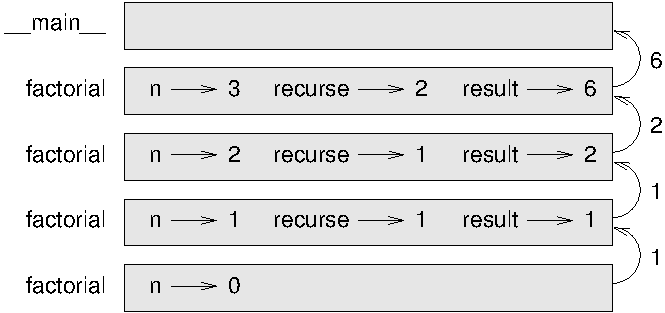
\includegraphics[scale=0.8]{figs/stack3.pdf}}
\caption{แผนภาพแบบกองซ้อน}
\label{fig.stack3}
\end{figure}

ค่าคืนกลับถูกแสดงว่ากำลังถูกส่งกลับขึ้นไปบนกอง (stack) ในแต่ละกรอบ ค่าคืนกลับ
คือ ค่าของ {\tt result} ซึ่งเป็นผลคูณของ {\tt n} และ {\tt recurse}
\index{function frame}
\index{frame}
\index{กรอบฟังก์ชัน}
\index{กรอบ}

ในกรอบสุดท้าย มันไม่มีตัวแปรเฉพาะที่ {\tt recurse} และ {\tt result} เพราะว่า
แขนงที่ทำให้มันเกิดขึ้นนั้นไม่ได้ทำงาน


\section{การปล่อยไปตามโชคชะตา } %(Leap of faith)}
\index{recursion}
\index{leap of faith}
\index{การเรียกซ้ำ}
\index{การปล่อยไปตามโชคชะตา}

การไล่ตามกระแสการดำเนินการเป็นหนทางหนึ่งที่จะอ่านโปรแกรม แต่มันก็สามารถทำให้เรารู้สึกท่วมท้นได้เร็ว
อีกทางเลือกหนึ่ง คือ สิ่งที่ผมเรียกว่า ``การปล่อยไปตามโชคชะตา (Leap of faith)'' เมื่อเรามาถึง
การเรียกฟังก์ชัน แทนที่จะไล่ตามกระแสการดำเนินการ เราจะ {\em สมมติ} ว่าฟังก์ชันทำงานได้อย่าง
ถูกต้อง และคืนค่าที่ถูกต้องกลับมาให้

ที่จริงแล้ว เราได้ฝึกการปล่อยไปตามโชคชะตามาแล้ว เมื่อเราใช้ฟังก์ชันพร้อมใช้ (built-in)
เมื่อเราเรียก {\tt math.cos} หรือ {\tt math.exp} เราไม่ได้สำรวจส่วนตัวของฟังก์ชันดังกล่าวเลย
เราแค่สมมติว่ามันทำงานได้ เพราะว่าคนที่เขียนฟังก์ชันพวกนี้เป็นโปรแกรมเมอร์ที่เก่ง

เป็นจริงเช่นเดียวกันเมื่อเราเรียกฟังก์ชันของเราเอง เช่น ในหัวข้อ~\ref{boolean} เราเขียนฟังก์ชันที่ชื่อว่า
\verb"is_divisible" ซึ่งหาว่าเลขหนึ่งถูกเลขอีกตัวหนึ่งหารลงตัวหรือไม่ เมื่อเรามั่นใจแล้ว
ว่าฟังก์ชันนี้น่าจะทำงานถูกต้อง---โดยการสำรวจโค้ดและทดสอบมัน---เราสามารถใช้ฟังก์ชัน
นี้ไปเลยโดยไม่ต้องดูส่วนของตัวฟังก์ชันอีก
\index{testing!leap of faith}
\index{การทดสอบ!การปล่อยไปตามโชคชะตา}

เป็นจริงเช่นเดียวกันกับโปรแกรมเรียกซ้ำ เมื่อเราทำการเรียกซ้ำ แทนที่เราจะไล่ตามกระแสการดำเนินการ
เราควรจะสมมติว่าการเรียกซ้ำนั้นทำงานได้ (คืนค่าที่ถูกต้องกลับมา) และจากนั้นให้ถามตัวเองว่า
``สมมติว่าเราสามารถหาค่าแฟกทอเรียบของ $n-1$ แล้ว เราจะสามารถคำนวณค่าแฟกทอเรียลของ $n$
ได้หรือเปล่า'' มันชัดเจนว่าเราสามารถทำได้ โดยการคูณค่า $n$ เข้าไป

แน่นอนว่ามันแปลกหน่อย ๆ ที่จะสมมติว่าฟังก์ชันมันทำงานได้ถูกต้อง เมื่อเรายังเขียนไม่เสร็จเลย
แต่มันก็เป็นเหตุผลที่ว่าทำไมเราถึงเรียกมันว่า การปล่อยไปตามโชคชะตา ยังไงล่ะ!


\section{อีกตัวอย่างหนึ่ง} % (One more example)}
\label{one.more.example}

\index{fibonacci function}
\index{function!fibonacci}
\index{ฟังก์ชันฟิโบนาชชี}
\index{ฟังก์ชัน!ฟิโบนาชชี}

หลังจากฟังก์ชัน {\tt factorial} แล้ว ตัวอย่างที่นิยมใช้ของฟังก์ชันทางคณิตศาสตร์แบบเรียกซ้ำ คือ ฟังก์ชัน {\tt fibonacci}
ซึ่งมีนิยามดังนี้ (ดู \url{http://en.wikipedia.org/wiki/Fibonacci_number}):
%
\begin{eqnarray*}
&& \mathrm{fibonacci}(0) = 0 \\
&& \mathrm{fibonacci}(1) = 1 \\
&& \mathrm{fibonacci}(n) = \mathrm{fibonacci}(n-1) + \mathrm{fibonacci}(n-2)
\end{eqnarray*}
%
เมื่อแปลมาเป็นไพธอนจะมีหน้าตาแบบนี้:

\begin{verbatim}
def fibonacci(n):
    if n == 0:
        return 0
    elif  n == 1:
        return 1
    else:
        return fibonacci(n-1) + fibonacci(n-2)
\end{verbatim}
%
ถ้าเราพยายามที่จะไล่ตามกระแสการดำเนินการตรงนี้ แม้แต่เป็นค่าน้อย ๆ ของ $n$ หัวของเราจะระเบิด
แต่จากหลักการปล่อยให้เป็นไปตามโชคชะตาแล้ว ถ้าเราสมมติว่าการเรียกซ้ำทั้งสองนั้นทำงาน
ได้อย่างถูกต้องแล้ว มันก็จะชัดเจนว่าเราจะได้ผลลัพธ์ที่ถูกต้องจากการบวกค่าทั้งสองเข้า
ด้วยกัน
\index{flow of execution}
\index{กระแสการดำเนินการ}


\section{การตรวจสอบชนิดของข้อมูล} % (Checking types)}
\label{guardian}

จะเกิดอะไรขึ้นถ้าเราเรียกฟังก์ชัน {\tt factorial} และผ่านค่า 1.5 เป็นอาร์กิวเมนต์?
\index{type checking}
\index{error checking}
\index{factorial function}
\index{RuntimeError}
\index{การตรวจสอบชนิดของข้อมูล}
\index{การตรวจสอบข้อผิดพลาด}
\index{ฟังก์ชันแฟกทอเรียล}
\index{ข้อผิดพลาดตอนโปรแกรมทำงาน}

\begin{verbatim}
>>> factorial(1.5)
RuntimeError: Maximum recursion depth exceeded
\end{verbatim}
% 
ดูเหมือนว่ามันเป็นการเรียกซ้ำไม่รู้จบ เป็นไปได้ยังไงกัน? ฟังก์ชันนี้มีกรณีฐาน---เมื่อ {\tt n == 0}
แต่ถ้า {\tt n} ไม่ใช่จำนวนเต็ม เราสามารถจะ {\em พลาด} การเจอกรณีฐาน และเรียกซ้ำไปชั่วนิรันดร์ได้
\index{infinite recursion}
\index{recursion!infinite}
\index{การเรียกซ้ำไม่รู้จบ}
\index{การเรียกซ้ำ!ไม่รู้จบ}

ในการเรียกซ้ำครั้งแรก ค่าของ {\tt n} คือ 0.5 ส่วนในครั้งถัดไปคือ -0.5
จากนั้น ค่ามันก็จะน้อยลงเรื่อย ๆ (เป็นลบมากขึ้น) แต่มันจะไม่มีวันเป็น 0

เรามีสองทางเลือก เราสามารถที่จะทำให้ฟังก์ชัน {\tt factorial} ครอบคลุมถึงเลขจุดลอย หรือเราสามารถ
ทำให้ {\tt factorial} ตรวจสอบชนิดของอาร์กิวเมนต์ได้ ทางเลือกแรก เรียกว่า ฟังก์ชันแกมม่า (gamma function)
และมันเกินขอบเขตของหนังสือเล่มนี้ ดังนั้น เราจะทำทางเลือกที่สอง
\index{gamma function}
\index{ฟังก์ชันแกมม่า}

เราสามารถใช้ฟังก์ชันพร้อมใช้ที่ชื่อว่า {\tt isinstance} เพื่อตรวจสอบชนิดของอาร์กิวเมนต์ ในเวลาเดียวกัน
เราสามารถตรวจสอบว่ามันเป็นจำนวนบวกหรือไม่ได้ด้วย
\index{isinstance function}
\index{function!isinstance}
\index{ฟังก์ชัน isinstance}
\index{ฟังก์ชัน!isinstance}

\begin{verbatim}
def factorial(n):
    if not isinstance(n, int):
        print('Factorial is only defined for integers.')
        return None
    elif n < 0:
        print('Factorial is not defined for negative integers.')
        return None
    elif n == 0:
        return 1
    else:
        return n * factorial(n-1)
\end{verbatim}
%
กรณีฐานแรกจัดการกับเลขที่ไม่ใช่จำนวนเต็ม; กรณีฐานที่สองจัดการกับจำนวนเต็มลบ ในทั้งสองกรณี
โปรแกรมพิมพ์ข้อความแจ้งและคืนค่าเป็น {\tt None} เพื่อระบุว่าบางสิ่งบางอย่างนั้นไม่ถูกต้อง:

\begin{verbatim}
>>> print(factorial('fred'))
Factorial is only defined for integers.
None
>>> print(factorial(-2))
Factorial is not defined for negative integers.
None
\end{verbatim}
% 
ถ้าเราสามารถผ่านการตรวจสอบทั้งสองอย่างได้ เรารู้ว่า $n$ เป็นจำนวนบวก หรือ ศูนย์
ดังนั้น เราสามารถพิสูจน์ได้ว่าการเรียกซ้ำนั้นจะสิ้นสุด
\index{guardian pattern}
\index{pattern!guardian}
\index{รูปแบบผู้พิทักษ์}
\index{รูปแบบ!ผู้พิทักษ์ }

โปรแกรมนี้สาธิตรูปแบบที่บางทีเรียกว่า {\bf ผู้พิทักษ์ (guardian)} เงื่อนไขสองข้อแรกทำตัว
เป็นผู้พิทักษ์ ป้องกันโค้ดจากค่าที่ทำให้เกิดข้อผิดพลาดขึ้นได้ ผู้พิทักษ์ทำให้การพิสูจน์
ความถูกต้องของโค้ดนั้นเป็นไปได้

ในหัวข้อที่~\ref{raise} เราจะเห็นทางเลือกที่ยืดหยุ่นกว่านี้ในการพิมพ์ข้อความแจ้งข้อผิดพลาด: 
การชูข้อยกเว้น (raising an exception)


\section{การดีบัก}
\label{factdebug}

การแตกโปรแกรมใหญ่ ๆ ให้เป็นฟังก์ชันเล็ก ๆ ทำให้เกิดจุดตรวจสอบโค้ด (checkpoints for debugging) โดยธรรมชาติ
ถ้าฟังก์ชันใดทำงานไม่ได้ มีความเป็นไปได้สามอย่างที่จะต้องพิจารณา:
\index{debugging} 
\index{การดีบัก}

\begin{itemize}

\item มีอะไรบางอย่างผิดปกติเกี่ยวกับอาร์กิวเมนต์ที่ได้รับมา; เงื่อนไขเบื้องต้นผิด

\item มีอะไรบางอย่างผิดปกติเกี่ยวกับฟังก์ชันเอง; เงื่อนไขลงท้ายผิด

\item มีอะไรบางอย่างผิดปกติเกี่ยวกับค่าคืนกลับ หรือเกี่ยวกับวิธีที่ค่านั้นถูกใช้

\end{itemize}

เพื่อที่จะตัดความเป็นไปได้ข้อแรกออกไป เราสามารถเพิ่มคำสั่ง {\tt print} ตอนเริ่มฟังก์ชัน
และแสดงค่าของพารามิเตอร์ต่าง ๆ (และอาจจะชนิดของข้อมูลด้วย) หรือเราสามารถเขียนโค้ดที่
ตรวจสอบเงื่อนไขเบื้องต้นโดยตรงเลย
\index{precondition}
\index{postcondition}
\index{เงื่อนไขเบื้องต้น}
\index{เงื่อนไขลงท้าย}

ถ้าพารามิเตอร์ก็ดูใช้ได้ดี ให้เพิ่มคำสั่ง {\tt print} ก่อนคำสั่ง return แต่ละอัน และแสดง
ค่าคืนกลับ  ถ้าเป็นไปได้ ให้ตรวจสอบผลลัพธ์โดยมือ พิจารณาการเรียกฟังก์ชันด้วยค่าที่ง่ายต่อ
การตรวจสอบผลลัพธ์ที่ถูกต้อง (เหมือนในหัวข้อที่~\ref{incremental.development})

ถ้าฟังก์ชันก็น่าจะทำงานถูกต้อง ให้ดูที่การเรียกฟังก์ชันเพื่อที่จะมั่นใจว่าค่าที่ถูกส่งคืนกลับมานั้น
ถูกนำมาใช้ได้อย่างถูกต้อง (หรือถูกนำมาใช้จริง ๆ!)
\index{flow of execution}
\index{กระแสการดำเนินการ}

การเพิ่มคำสั่ง print ในตอนเริ่มและจบของฟังก์ชัน ช่วยให้กระแสการดำเนินการนั้นชัดเจนขึ้น เช่น นี่เป็น
เวอร์ชันอันหนึ่งของฟังก์ชัน {\tt factorial} ที่มีคำสั่ง print อยู่:

\begin{verbatim}
def factorial(n):
    space = ' ' * (4 * n)
    print(space, 'factorial', n)
    if n == 0:
        print(space, 'returning 1')
        return 1
    else:
        recurse = factorial(n-1)
        result = n * recurse
        print(space, 'returning', result)
        return result
\end{verbatim}
%
{\tt space} เป็นสายอักขระของอักขระเว้นวรรค ที่ควบคุมการย่อหน้าของเอ้าต์พุต 
นี่คือผลการทำงานของ {\tt factorial(4)}:

\begin{verbatim}
                 factorial 4
             factorial 3
         factorial 2
     factorial 1
 factorial 0
 returning 1
     returning 1
         returning 2
             returning 6
                 returning 24
\end{verbatim}
%
ถ้าเรางงเกี่ยวกับกระแสการดำเนินการ เอ้าต์พุตลักษณะนี้จะมีประโยชน์ มันใช้เวลาระยะหนึ่งในการพัฒนา
นั่งร้านที่มีประสิทธิภาพ แต่การสร้างนั่งร้านขึ้นมาเล็กน้อยนั้นสามารถประหยัดการดีบักได้มาก


\section{อภิธานศัพท์} % (Glossary)}

\begin{description}

\item[ตัวแปรชั่วคราว (temporary variable):]  ตัวแปรที่ใช้เก็บค่าระหว่างทางในการคำนวณที่ซับซ้อน
\index{temporary variable}
\index{variable!temporary}
\index{ตัวแปรชั่วคราว}
\index{ตัวแปร!ชั่วคราว}

\item[โค้ดตาย (dead code):] ส่วนของโปรแกรมที่ไม่มีวันทำงาน บ่อยครั้งเพราะมันอยู่หลังจากคำสั่ง {\tt return}
\index{dead code}
\index{โค้ดตาย}

\item[การพัฒนาแบบเพิ่มส่วน (incremental development):]  แผนการพัฒนาโปรแกรมที่มุ่งหลีกเลี่ยงการดีบัก โดยการคูณค่า
เพิ่มและทดสอบโค้ดทีละน้อย 
\index{incremental development}
\index{การพัฒนาแบบเพิ่มส่วน}

\item[นั่งร้าน (scaffolding):]  โค้ดที่ใช้ในระหว่างการพัฒนาโปรแกรม แต่ไม่ใช่ส่วนหนึ่งของโปรแกรมเวอร์ชันสุดท้าย
\index{scaffolding}
\index{นั่งร้าน}

\item[ผู้พิทักษ์ (guardian):]  รูปแบบการเขียนโปรแกรมที่ใช้คำสั่งเงื่อนไขเพื่อตรวจสอบและจัดการกับเหตุการณ์ที่อาจจะทำให้เกิดข้อผิดพลาด
\index{guardian pattern}
\index{pattern!guardian}
\index{รูปแบบผู้พิทักษ์}
\index{รูปแบบ!ผู้พิทักษ์}

\end{description}


\section{แบบฝึกหัด}

\begin{exercise}

ให้เขียนแผนภาพแบบกองซ้อนสำหรับโปรแกรมต่อไปนี้ โปรแกรมนี้พิมพ์อะไรออกมา?
\index{stack diagram}
\index{แผนภาพแบบกองซ้อน}

\begin{verbatim}
def b(z):
    prod = a(z, z)
    print(z, prod)
    return prod

def a(x, y):
    x = x + 1
    return x * y

def c(x, y, z):
    total = x + y + z
    square = b(total)**2
    return square

x = 1
y = x + 1
print(c(x, y+3, x+y))
\end{verbatim}

\end{exercise}


\begin{exercise}
\label{ackermann}

ฟังก์ชันแอคเคอร์มานน์, $A(m, n)$, นิยามว่า:

\begin{eqnarray*}
A(m, n) = \begin{cases} 
              n+1 & \mbox{if } m = 0 \\ 
        A(m-1, 1) & \mbox{if } m > 0 \mbox{ and } n = 0 \\ 
A(m-1, A(m, n-1)) & \mbox{if } m > 0 \mbox{ and } n > 0.
\end{cases} 
\end{eqnarray*}
%
ดูเพิ่มเติมที่ \url{http://en.wikipedia.org/wiki/Ackermann_function}.

ให้เขียนฟังก์ชันที่ชื่อว่า {\tt ack} ซึ่งประเมินค่าของฟังก์ชันแอคเคอร์มานน์ ใช้ฟังก์ชันของเราเพื่อหา
{\tt ack(3, 4)} ซึ่งควรจะมีค่าเป็น 125  เกิดอะไรขึ้นกับค่าของ {\tt m} และ {\tt n} ที่มากกว่านี้?
เฉลย: \url{http://thinkpython2.com/code/ackermann.py}.
\index{Ackermann function}
\index{function!ack}
\index{ฟังก์ชันแอคเคอร์มานน์}
\index{ฟังก์ชัน!ack}

\end{exercise}


\begin{exercise}
\label{palindrome}

พาลินโดรม (palindrome) คือ คำที่สะกดเหมือนกันทั้งเวลาเริ่มอ่านจากข้างหน้าและเริ่มอ่านจากข้างหลัง
เช่น ``noon'' และ ``redivider''  ถ้าคิดแบบการเรียกซ้ำ คำใด ๆ เป็นพาลินโดรม เมื่ออักษรตัวแรก
และตัวสุดท้ายเป็นตัวเดียวกัน และตรงกลางเป็นพาลินโดรม
\index{palindrome}
\index{พาลินโดรม}

ต่อไปนี้ คือ ฟังก์ชันที่รับอาร์กิวเมนต์ที่เป็นสายอักขระและส่งค่าคืนกลับเป็น อักษรตัวแรก อักษรตัวสุดท้าย และกลุ่มอักษรตรงกลาง:

\begin{verbatim}
def first(word):
    return word[0]

def last(word):
    return word[-1]

def middle(word):
    return word[1:-1]
\end{verbatim}
%
เราจะเห็นว่ามันทำงานอย่างไรในบทที่~\ref{strings}

\begin{enumerate}

\item ให้พิมพ์ฟังก์ชันเหล่านี้ลงในไฟล์ชื่อว่า {\tt palindrome.py} และทดสอบมันดู
จะเกิดอะไรขึ้นถ้าเราเรียก {\tt middle} ด้วยสายอักขระที่มีสองตัวอักษร? แล้วถ้าเรียกด้วยตัวเดียวล่ะ?
แล้วถ้าเป็นสายอักขระว่าง (empty string) ซึ่งเขียนว่า\verb"''" และไม่มีตัวอักษรเลยล่ะ?

\item ให้เขียนฟังก์ชันชื่อว่า \verb"is_palindrome" ซึ่งรับอาร์กิวเมนต์ที่เป็นสายอักขระ และคืนค่า {\tt True} 
ถ้าเป็นพาลินโดรม และ {\tt False} ถ้าไม่ใช่  จำไว้ว่าเราสามารถใช้ฟังก์ชันพร้อมใช้ {\tt len} 
เพื่อที่จะตรวจสอบความยาวของสายอักขระ

\end{enumerate}

เฉลย: \url{http://thinkpython2.com/code/palindrome_soln.py}.

\end{exercise}

\begin{exercise}

เลข $a$ เป็นค่ายกกำลังของ $b$ หากมันสามารถหารด้วย $b$ ลงตัว และ $a/b$ เป็นค่ายกกำลังของ $b$
ให้เขียนการเรียกฟังก์ชัน \verb"is_power" ซึ่งรับพารามิเตอร์ {\tt a} และ {\tt b}
และคืนค่า {\tt True} ถ้า {\tt a} เป็นค่ายกกำลังของ {\tt b}. 
หมายเหตุ: เราจะต้องคิดเรื่องกรณีฐานด้วย

\end{exercise}


\begin{exercise}
\index{greatest common divisor (GCD)}
\index{GCD (greatest common divisor)}
\index{ตัวหารร่วมมาก (ห.ร.ม.)}
\index{ห.ร.ม. (ตัวหารร่วมมาก)}

ตัวหารร่วมมาก (ห.ร.ม.) หรือ the greatest common divisor (GCD) ของ $a$ และ $b$
คือเลขจำนวนที่มากที่สุดที่สามารถหารพวกมันได้โดยไม่มีเศษ 

วิธีหนึ่งที่จะหาค่า ห.ร.ม. ของเลขสองตัวมาจากข้อสังเกตที่ว่า ถ้า $r$ เป็นเศษของการหาร
เมื่อ $a$ ถูกหารด้วย $b$ แล้ว $gcd(a, b) = gcd(b, r)$
สำหรับกรณีฐาน เราสามารถใช้ $gcd(a, 0) = a$.

ให้เขียนฟังก์ชันที่ชื่อว่า \verb"gcd" ซึ่งรับพารามิเตอร์ {\tt a} และ {\tt b} และคืนค่า
ตัวหารร่วมมาก

เครดิต: แบบฝึกหัดนี้มาจากตัวอย่างจากหนังสือของ Abelson และ Sussman ชื่อว่า 
{\em Structure and Interpretation of Computer Programs}

\end{exercise}



\chapter{การวนซ้ำ} % (Iteration)}

เนื้อหาในบทนี้เกี่ยวกับการวนซ้ำ ซึ่งเป็นความสามารถในการรันก้อนชุดคำสั่งซ้ำไปมา เราได้เห็น
การวนซ้ำแบบหนึ่งไปแล้วโดยการใช้การเรียกซ้ำ ในหัวข้อที่~\ref{recursion} เราได้เห็นอีกแบบ
โดยใช้ลูป {\tt for} ในหัวข้อที่~\ref{repetition} ในบทนี้ เราจะเห็นอีกแบบ
โดยการใช้คำสั่ง {\tt while}
แต่ก่อนอื่น ผมอยากจะพูดอะไรนิดหน่อยเกี่ยวกับการกำหนดค่าให้ตัวแปร

\section{การกำหนดค่าให้ใหม่ } %(Reassignment)}
\index{assignment}
\index{statement!assignment}
\index{reassignment}
\index{การกำหนดค่า}
\index{คำสั่ง!การกำหนดค่า}
\index{การกำหนดค่าให้ใหม่ }

เราอาจจะค้นพบแล้วว่า เราสามารถกำหนดค่าให้ตัวแปรตัวเดิมได้มากกว่าหนึ่งครั้ง การกำหนดค่าครั้งใหม่
ทำให้ตัวแปรนั้นอ้างอิงไปที่ค่าใหม่ (และหยุดอ้างอิงไปที่ค่าเก่า)

\begin{verbatim}
>>> x = 5
>>> x
5
>>> x = 7
>>> x
7
\end{verbatim}
%
ครั้งแรกที่เราแสดงค่า {\tt x} มันเป็น 5; พอครั้งที่สอง มันเป็น 7

รูปที่~\ref{fig.assign2} แสดงให้เห็นว่าการกำหนดค่าให้ใหม่เป็นอย่างไรในแผนภาพสถานะ 
\index{state diagram} \index{diagram!state}
\index{แผนภาพสถานะ} \index{แผนภาพ!สถานะ}

ถึงตรงนี้ ผมอยากจะพูดถึงจุดที่สับสนกันมาก
เพราะว่าไพธอนใช้เครื่องหมายเท่ากับ ({\tt =}) เพื่อการกำหนดค่า มันเลยทำให้เราอยากจะแปล
คำสั่งเช่น {\tt a = b} ว่าเป็นการแสดงการเท่ากันทางตรรกะ; นั่นคือ การที่บอกว่า 
{\tt a} และ {\tt b} นั้นเท่ากัน  แต่การแปลความแบบนี้มันผิด
\index{equality and assignment}
\index{การเท่ากัน และ การกำหนดค่า}

อย่างแรก การเท่ากันเป็นความสัมพันธ์แบบสมมาตร แต่การกำหนดค่าไม่ใช่ เช่น ในคณิตศาสตร์
ถ้า $a=7$ แล้ว $7=a$  แต่ในไพธอน คำสั่ง {\tt a = 7} นั้นทำได้ และ {\tt 7 = a} นั้นทำไม่ได้

นอกจากนี้ ในคณิตศาสตร์ การเท่ากันทางตรรกะมีค่าเป็น จริง หรือ เท็จ ตลอดเวลา ถ้า $a=b$ ในตอนนี้ 
แล้ว $a$ จะเท่ากับ $b$ เสมอ  ในไพธอน การกำหนดค่าอาจจะทำให้ตัวแปรสองตัวมีค่าเท่ากัน 
แต่มันจะไม่เป็นแบบนั้นตลอดไป:

\begin{verbatim}
>>> a = 5
>>> b = a    # a and b are now equal
>>> a = 3    # a and b are no longer equal
>>> b
5
\end{verbatim}
% 
บรรทัดที่สามเปลี่ยนค่าของ {\tt a} แต่ไม่เปลี่ยนค่าของ {\tt b} ดังนั้น มันจึงไม่เท่ากันแล้ว

การกำหนดค่าให้ใหม่นั้นบ่อยครั้งมีประโยชน์ แต่เราควรจะต้องใช้มันอย่างระมัดระวัง ถ้า
ค่าของตัวแปรนั้นเปลี่ยนบ่อย ๆ มันอาจจะทำให้อ่านโค้ดและดีบักได้ยากขึ้น

\begin{figure}
\centerline
{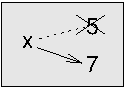
\includegraphics[scale=0.8]{figs/assign2.pdf}}
\caption{แผนภาพสถานะของตัวแปร}
\label{fig.assign2}
\end{figure}



\section{การปรับค่าตัวแปร} % (Updating variables)}
\label{update}

\index{update}
\index{variable!updating}
\index{การปรับค่า}
\index{ตัวแปร!updating}

% A common kind of reassignment is an {\bf update},
% where the new value of the variable depends on the old.
การกำหนดค่าให้ใหม่ที่ทำเป็นปกติ คือ {\bf การปรับค่าตัวแปร (update)} โดยที่
ค่าใหม่จะขึ้นอยู่กับค่าเก่า


\begin{verbatim}
>>> x = x + 1
\end{verbatim}
%
มันหมายความว่า ``เอาค่าปัจจุบันของ {\tt x}, บวกหนึ่ง, แล้วปรับค่า {\tt x} ให้เป็นค่าใหม่''

ถ้าเราพยายามที่จะปรับค่าตัวแปรที่ไม่มีอยู่จริง เราจะได้ข้อผิดพลาด เพราะว่าไพธอนจะประเมินค่าทางขวา 
ก่อนที่จะกำหนดค่าให้ตัวแปร {\tt x}:

\begin{verbatim}
>>> x = x + 1
NameError: name 'x' is not defined
\end{verbatim}
%
ก่อนที่เราจะสามารถปรับค่าตัวแปรได้ เราจะต้อง {\bf ให้ค่าเริ่มต้น (initialize)} กับมันก่อน
โดยปกติแล้ว จะใช้การกำหนดค่าแบบง่าย ๆ:
\index{initialization (before update)}
\index{การให้ค่าเริ่มต้น (ก่อนการปรับค่า)}

\begin{verbatim}
>>> x = 0
>>> x = x + 1
\end{verbatim}
%
การปรับค่าตัวแปรโดยการบวก 1 เข้าไปเรียกว่า {\bf การเพิ่มค่า (increment)};
ส่วนการลบออก 1 เรียกว่า {\bf การลดค่า (decrement)}
\index{increment}
\index{decrement}
\index{การเพิ่มค่า}
\index{การลดค่า}



\section{คำสั่ง {\tt while}}
\index{statement!while}
\index{while loop}
\index{loop!while}
\index{iteration}
\index{คำสั่ง!while}
\index{ลูป while}
\index{ลูป!while}
\index{การวนซ้ำ}

บ่อยครั้งที่คอมพิวเตอร์เคยชินกับการทำงานซ้ำ ๆ แบบอัตโนมัติ การทำงานอะไรที่เหมือน ๆ 
กันโดยไม่มีข้อผิดพลาด คือ สิ่งที่คอมพิวเตอร์สามารถทำงานได้ดี และคนทำได้ไม่ดีนัก
ในโปรแกรมคอมพิวเตอร์ การทำงานซ้ำ ๆ เรียกอีกอย่างหนึ่งว่า {\bf การวนซ้ำ (iteration)}

เราได้เห็นฟังก์ชันไปแล้วสองฟังก์ชัน, {\tt countdown} และ \verb"print_n", ที่วนซ้ำโดยการใช้การเรียกซ้ำ
เพราะว่าการวนซ้ำเป็นอะไรที่ปกติธรรมดามาก ไพธอนจึงเตรียมคุณลักษณะของภาษาที่ทำให้มันง่ายขึ้น
หนึ่งคือคำสั่ง {\tt for} ที่เราเห็นในหัวข้อที่~\ref{repetition} เราจะกลับไปพูดเรื่องนั้นทีหลัง 

อีกคำสั่งหนึ่ง คือ คำสั่ง {\tt while} นี่คือเวอร์ชันของฟังก์ชัน {\tt countdown} ที่ใช้คำสั่ง {\tt while}:

\begin{verbatim}
def countdown(n):
    while n > 0:
        print(n)
        n = n - 1
    print('Blastoff!')
\end{verbatim}
%
เราสามารถอ่านคำสั่ง {\tt while} เหมือนกับว่าเป็นภาษาอังกฤษทั่วไปเลย มันหมายความว่า
``ในขณะที่ {\tt n} มีค่ามากกว่า 0, ให้แสดงค่าของ {\tt n} และจากนั้นให้ลดค่า {\tt n} ลงหนึ่ง
เมื่อเราได้ค่าเป็น 0 แล้ว ให้แสดงคำว่า {\tt Blastoff!}''
\index{flow of execution}
\index{กระแสการดำเนินการ}

นี่คือกระแสการดำเนินการสำหรับคำสั่ง {\tt while} อย่างเป็นทางการ:

\begin{enumerate}

\item ประเมินว่าเงื่อนไขเป็น จริง หรือ เท็จ

\item ถ้าเป็นเท็จ ให้ออกจากคำสั่ง {\tt while}
และทำคำสั่งถัดไปเลย

\item ถ้าเงื่อนไขเป็นจริง ให้รันส่วนตัวของคำสั่ง while ให้ครบ
แล้วกลับไปที่ขั้นตอนที่ 1

\end{enumerate}

กระแสการทำงานแบบนี้เรียกว่า ลูป (loop) เพราะว่าขั้นตอนที่ 3 จะทำการวนกลับ (ลูปกลับ) ย้อนไปข้างบน

\index{condition}
\index{loop}
\index{body}
\index{เงื่อนไข}
\index{ลูป}
\index{ส่วนตัว}

ส่วนที่เป็นตัวของลูปควรจะเปลี่ยนค่าของตัวแปรอย่างน้อยหนึ่งตัว เพื่อที่จะทำให้เงื่อนไขกลายเป็น 
เท็จ (False) ในที่สุด และทำให้ลูปหยุดทำงาน  ไม่เช่นนั้น ลูปจะทำงานไปเรื่อย ๆ ชั่วนิรันดร์ ซึ่งเรียกว่า
{\bf ลูปไม่รู้จบ (infinite loop)}  แหล่งของความบันเทิงแบบไม่สิ้นสุดของนักวิทยาการคอมพิวเตอร์
คือ การสังเกตพบว่า วิธีใช้งานของยาสระผม คือ ``สระให้เกิดฟอง, ล้างออก, ทำซ้ำอีกรอบ'' นั้นเป็นลูปไม่รู้จบ
\index{infinite loop}
\index{loop!infinite}
\index{ลูปไม่รู้จบ}
\index{ลูป!ไม่รู้จบ}

ในกรณีของฟังก์ชัน {\tt countdown} เราสามารถพิสูจน์ได้ว่า ลูปจะหยุดทำงาน: ถ้า {\tt n} เป็นศูนย์หรือลบ
ลูปจะไม่ทำงานเลย ไม่เช่นนั้น ค่า {\tt n} จะน้อยลงในแต่ละรอบของการลูป ทำให้ในที่สุด เราก็จะต้องได้ 0

สำหรับลูปอื่น ๆ บางลูป มันไม่ง่ายนักที่จะพิสูจน์แบบนั้น เช่น:

\begin{verbatim}
def sequence(n):
    while n != 1:
        print(n)
        if n % 2 == 0:        # n is even เลขคู่
            n = n / 2
        else:                 # n is odd เลขคี่
            n = n*3 + 1
\end{verbatim}
%
เงื่อนไขสำหรับลูปนี้ คือ {\tt n != 1} ดังนั้น ลูปจะวนไปเรื่อย ๆ จนกว่า {\tt n} เป็น {\tt 1}
ซึ่งทำให้เงื่อนไขนั้นเป็นเท็จ

แต่ละครั้งที่ทำลูป โปรแกรมจะเอ้าต์พุตค่าของ {\tt n} และจากนั้นจะตรวจสอบว่ามันเป็นจำนวนคู่หรือจำนวนคี่
ถ้าเป็นจำนวนคู่ {\tt n} จะถูกหารด้วย 2 แต่ถ้าเป็นจำนวนคี่ ค่าของ {\tt n} จะถูกแทนด้วย {\tt n*3 + 1}
เช่น ถ้าอาร์กิวเมนต์ที่ผ่านเข้าไปใน {\tt sequence} คือ 3 ผลของ {\tt n} จะเป็น
3, 10, 5, 16, 8, 4, 2, 1

เนื่องจากบางครั้ง {\tt n} มีค่าเพิ่มขึ้นและบางครั้งมีค่าลดลง เลยพิสูจน์ไม่ได้อย่างชัดเจนว่า {\tt n}
จะมีค่าถึง 1 หรือไม่ หรือโปรแกรมจะหยุดทำงานหรือไม่ สำหรับเฉพาะบางค่าของ {\tt n} เราสามารถ
พิสูจน์ได้ว่าโปรแกรมจะหยุดทำงาน เช่น ถ้าค่าเริ่มต้นเป็นค่าที่ยกกำลังสอง {\tt n} 
จะเป็นจำนวนคู่ในทุก ๆ รอบของลูปจนกระทั่งถึงค่า 1  ตัวอย่างที่แล้วจบด้วยลำดับอย่างว่าโดยเริ่มที่ค่า 16
\index{Collatz conjecture}
\index{ข้อความคาดการณ์ของคอลลาทซ์}

คำถามที่ยาก คือ เราสามารถพิสูจน์ได้หรือไม่ว่าโปรแกรมจะจบสำหรับค่า {\tt n} ที่เป็นบวก {\em ทุกค่า}
จนถึงตอนนี้ ไม่มีใครสามารถพิสูจน์ว่ามันได้ {\em หรือ} พิสูจน์ว่ามันไม่ได้! (ให้ดู
\url{http://en.wikipedia.org/wiki/Collatz_conjecture}.)

เพื่อเป็นการฝึกทำ ให้เขียนฟังก์ชัน \verb"print_n" ใหม่จากหัวข้อที่~\ref{recursion}
โดยใช้การวนซ้ำ (iteration) แทนการใช้การเรียกซ้ำ (recursion)


\section{คำสั่ง {\tt break}}
\index{break statement}
\index{statement!break}
\index{คำสั่ง break}
\index{คำสั่ง!break}

บางครั้ง เราไม่รู้ว่าเมื่อไหร่จะต้องหยุดลูป จนกระทั่งเรามาถึงครึ่งทางของลูป ในกรณีนั้น
เราสามารถใช้คำสั่ง {\tt break} ในการกระโดดออกจากลูป

ตัวอย่างเช่น สมมติว่าเราต้องเอาอินพุตมาจากผู้ใช้จนกระทั่งเขาพิมพ์เข้ามาว่า {\tt done}
เราสามารถเขียนว่า:

\begin{verbatim}
while True:
    line = input('> ')
    if line == 'done':
        break
    print(line)

print('Done!')
\end{verbatim}
%
เงื่อนไขของลูปนี้ คือ {\tt True} ซึ่งจะเป็นจริงเสมอ ดังนั้น ลูปจะรันจนกว่าจะเจอ
คำสั่ง break

ในแต่ละรอบของลูป โปรแกรมจะขอข้อมูลจากผู้ใช้โดยใช้เครื่องหมายวงเล็บสามเหลี่ยมแบบเปิด (<) 
ถ้าผู้ใช้พิมพ์เข้ามาว่า {\tt done} คำสั่ง {\tt break} จะทำให้ออกจากลูป  ไม่เช่นนั้น
โปรแกรมจะสะท้อนสิ่งที่ผู้ใช้พิมพ์เข้ามา แล้วก็กลับไปยังข้างบนสุดของลูป นี่คือตัวอย่างการทำงาน:

\begin{verbatim}
> not done
not done
> done
Done!
\end{verbatim}
% 
การเขียนลูป {\tt while} แบบนี้เป็นเรื่องปกติ เพราะว่าเราสามารถตรวจสอบเงื่อนไข
ที่ไหนก็ได้ในลูป (ไม่เพียงแค่ในส่วนบนสุดของลูป) และเราสามารถยืนยันเงื่อนไขการหยุดได้
(``หยุดเมื่อสิ่งนี้เกิดขึ้น'') แทนที่จะบอกในทางลบ (``ทำงานไปเรื่อย ๆ จนกว่าสิ่งนั้นจะเกิด'')


\section{รากที่สอง} % (Square roots)}
\label{squareroot}
\index{square root}
\index{รากที่สอง}

ลูปมักถูกใช้ในโปรแกรมที่คำนวณผลลัพธ์เชิงตัวเลข โดยการเริ่มด้วยค่าประมาณ
และวนซ้ำเพื่อทำคำตอบให้ดีขึ้น
\index{Newton's method}
\index{วิธีของนิวตัน}

ตัวอย่างเช่น วิธีหนึ่งของการคำนวณรากที่สอง คือ วิธีของนิวตัน (Newton's method)
สมมติว่าเราต้องการจะหารากที่สองของ $a$ ถ้าเราเริ่มด้วยค่าประมาณสักอย่าง, $x$, เรา
สามารถคำนวณค่าประมาณที่ดีกว่าเดิมโดยใช้สูตรต่อไปนี้:

\[ y = \frac{x + a/x}{2} \]
%
ตัวอย่างเช่น ถ้า $a$ คือ 4 และ $x$ คือ 3

\begin{verbatim}
>>> a = 4
>>> x = 3
>>> y = (x + a/x) / 2
>>> y
2.16666666667
\end{verbatim}
%
ผลลัพธ์ที่ได้จะใกล้เคียงกับคำตอบที่ถูกมากขึ้น ($\sqrt{4} = 2$) ถ้าเราทำกระบวนการนี้ซ้ำ
ด้วยการประมาณค่าใหม่ มันก็จะใกล้เข้าไปอีก:

\begin{verbatim}
>>> x = y
>>> y = (x + a/x) / 2
>>> y
2.00641025641
\end{verbatim}
%
หลังจากการปรับค่าอีกสองสามครั้ง ค่าประมาณก็เกือบจะเป๊ะ:
\index{update}
\index{การปรับค่า}

\begin{verbatim}
>>> x = y
>>> y = (x + a/x) / 2
>>> y
2.00001024003
>>> x = y
>>> y = (x + a/x) / 2
>>> y
2.00000000003
\end{verbatim}
%
โดยทั่วไปแล้ว เราไม่รู้ก่อนว่าจะต้องทำกี่ขั้นตอนจนกว่าจะได้คำตอบที่ถูกต้อง แต่เรารู้
เมื่อเราได้ค่านั้นมาแล้วเพราะว่าค่าประมาณนั้นไม่เปลี่ยนแล้ว:

\begin{verbatim}
>>> x = y
>>> y = (x + a/x) / 2
>>> y
2.0
>>> x = y
>>> y = (x + a/x) / 2
>>> y
2.0
\end{verbatim}
%
เมื่อ {\tt y == x} เราสามารถหยุดได้ นี่คือลูปที่เริ่มด้วยค่าประมาณการเริ่มต้น, {\tt x},
และปรับค่าให้ดีขึ้นเรื่อย ๆ จนกระทั่งมันหยุดเปลี่ยน:

\begin{verbatim}
while True:
    print(x)
    y = (x + a/x) / 2
    if y == x:
        break
    x = y
\end{verbatim}
%
สำหรับค่า {\tt a} ส่วนมาก วิธีนี้ทำงานได้ดี แต่โดยทั่วไปแล้วมันอันตรายถ้าจะทดสอบ
การเท่ากันของค่าจุดลอย {\tt float} ค่าจุดลอยเป็นเพียงแค่ค่าประมาณ: จำนวนตรรกยะส่วนมาก
เช่น $1/3$ และอตรรกยะ เช่น $\sqrt{2}$ ไม่สามารถแทนให้ตรงเป๊ะด้วยข้อมูลชนิด {\tt float}
\index{floating-point}
\index{epsilon}
\index{จุดลอย}
\index{เอปซิลอน}

แทนที่จะตรวจสอบว่า {\tt x} และ {\tt y} เท่ากันเป๊ะ มันปลอดภัยกว่าที่จะใช้
ฟังก์ชันพร้อมใช้ {\tt abs} เพื่อคำนวณหาค่าสัมบูรณ์, หรือขนาด, ของความต่างระหว่าง
สองค่านี้:

\begin{verbatim}
    if abs(y-x) < epsilon:
        break
\end{verbatim}
%
โดยที่ \verb"epsilon" มีค่าเช่น {\tt 0.0000001} ซึ่งกำหนดว่าใกล้เท่าไหร่
จึงจะเพียงพอ


\section{อัลกอริทึม} % (Algorithms)}
\index{algorithm}
\index{อัลกอริทึม}

วิธีของนิวตัน (Newton's method) เป็นตัวอย่างของ {\bf อัลกอริทึม (algorithm)}: 
มันคือกระบวนการทางกลไกสำหรับแก้ปัญหาของหมวดหมู่หนึ่ง ๆ (ในกรณีนี้ การคำนวณรากที่สอง) 

เพื่อที่จะเข้าใจว่า อัลกอริทึม คืออะไร มันอาจจะช่วยโดยการเริ่มด้วยบางสิ่งที่ไม่ใช่อัลกอริทึม
เมื่อเราเรียนรู้ที่จะคูณเลขหลักเดียว เราอาจจะจำสูตรคูณ มันทำให้เราต้องท่องจำคำตอบ 100 
อย่างโดยเฉพาะ ความรู้แบบนี้ไม่ใช่อัลกอริทึม

แต่ถ้าเรา ``ขี้เกียจ' เราอาจจะเรียนรู้เทคนิคพิเศษสองสามอย่าง เช่น ในการที่จะหาผลคูณ
ของ $n$ และ 9 เราสามารถเขียน $n-1$ เป็นเลขหลักแรก และ $10-n$ เป็นเลขหลักที่สอง
เทคนิคนี้เป็นการแก้ปัญหาแบบครอบคลุมสำหรับการคูณเลขหลักเดียวตัวไหนก็ได้กับ 9
นี่คือ อัลกอริทึม!
\index{addition with carrying}
\index{carrying, addition with}
\index{subtraction!with borrowing}
\index{borrowing, subtraction with}
\index{การบวกด้วยการทด}
\index{การทด, การบวกด้วย}
\index{การลบ!ด้วยการยืม}
\index{การยืม, การลบด้วย}

ในทำนองเดียวกัน เทคนิคที่เราเรียนรู้สำหรับการบวกและลบแบบทดยืม และการหารยาวล้วนเป็น 
อัลกอริทึม ลักษณะหนึ่งของอัลกอริทึม คือ มันไม่ต้องการความฉลาดในการทำงาน มันเป็น
กลไกที่แต่ละขั้นตอนนั้นทำต่อ ๆ กันไปโดยอ้างอิงจากกฎเกณฑ์ง่าย ๆ ชุดหนึ่ง 

การทำงานตามอัลกอริทึมมันน่าเบื่อ แต่การออกแบบนั้นน่าสนใจ ประเทืองปัญญา และเป็น
ศูนย์กลางของวิทยาการคอมพิวเตอร์

บางสิ่งที่ผู้คนทำตามธรรมชาติโดยไม่ยากหรือไม่ต้องคิด เป็นสิ่งที่ยากที่สุดในการเขียนออกมาเป็น
อัลกอริทึม การทำความเข้าใจภาษาธรรมชาติ (natural language) เป็นตัวอย่างที่ดี
เราทุกคนเข้าใจมัน แต่จนกระทั่งบัดนี้ ไม่มีใครสามารถจะอธิบายได้ว่าเราทำมันได้ {\em อย่างไร}
อย่างน้อยก็ไม่ใช่ในรูปแบบของอัลกอริทึม


\section{การดีบัก}
\label{bisectbug}

เมื่อเราเริ่มเขียนโปรแกรมที่ใหญ่ขึ้น เราอาจจะใช้เวลาในการดีบักมากขึ้น โค้ดที่มากขึ้น 
หมายความว่า โอกาสที่มากขึ้นที่จะเกิดข้อผิดพลาด และมีหลายตำแหน่งมากขึ้นที่บัก
ซ่อนอยู่
\index{debugging!by bisection}
\index{bisection, debugging by}
\index{การดีบัก!โดยการตัดครึ่งส่วนn}
\index{การตัดครึ่งส่วน, การดีบักโดย}

ทางหนึ่งที่จะลดเวลาการดีบัก คือ ``การดีบักโดยการตัดครึ่งส่วน'' เช่น ถ้าในโปรแกรมมี
100 บรรทัด แล้วเราตรวจสอบไปทีละบรรทัด มันก็จะใช้ 100 ขั้นตอน

แทนที่จะทำแบบนั้น ให้แบ่งปัญหาลงครึ่งหนึ่ง ให้ดูแถว ๆ ตรงกลางของโปรแกรม 
หาค่าระหว่างทางที่เราสามารถตรวจสอบได้ เพิ่มคำสั่ง {\tt print}  (หรืออะไรสักอย่าง 
ที่สามารถทำให้เราตรวจสอบความถูกต้องได้) และรันโปรแกรม

ถ้าตรงกลางโปรแกรมมันผิด จะต้องมีปัญหาที่ครึ่งแรกของโปรแกรมแน่ ๆ แต่ถ้ามันถูก ปัญหา
จะอยู่ที่ครึ่งหลังของโปรแกรม

ทุกครั้งที่เราทำการตรวจสอบแบบนี้ เราจะแบ่งครึ่งจำนวนบรรทัดที่เราต้องค้นหา หลังจากผ่านไป
ุหกขั้นตอนแล้ว (ซึ่งน้อยกว่า 100 ขั้นตอน) เราจะเหลือแค่หนึ่งหรือสองบรรทัดเท่านั้น อย่างน้อย
ก็ตามทฤษฎี 

ในทางปฏิบัติ มันไม่ค่อยชัดเท่าไหร่ว่า ``กึ่งกลางโปรแกรม'' คืออะไร และอาจจะไม่
สามารถตรวจสอบมันได้ มันไม่ค่อยเข้าท่าเท่าไหร่ที่จะนับบรรทัดและหาจุดกึ่งกลางเป๊ะ 
แทนที่จะทำแบบนั้น ให้คิดว่าตำแหน่งใดในโปรแกรมที่อาจจะมีข้อผิดพลาด และตรงไหน
ที่มันตรวจสอบได้ง่าย จากนั้นให้เลือกมาจุดหนึ่งซึ่งเราคิดว่ามีโอกาสเท่า ๆ กันที่จะเกิดบัก
ก่อนหน้าและหลังจากจุดนั้น


\section{อภิธานศัพท์}

\begin{description}

\item[การกำหนดค่าใหม่ (reassignment):] การกำหนดค่าใหม่ให้ตัวแปรที่มีอยู่แล้ว
\index{reassignment}
\index{การกำหนดค่าใหม่}

\item[การปรับค่า (update):] คำสั่งที่ทำให้ค่าใหม่ของตัวแปรนั้นขึ้นอยู่กับค่าเก่า
\index{update}
\index{การปรับค่า}

\item[การให้ค่าตั้งต้น (initialization):] การกำหนดค่าเริ่มต้นให้ตัวแปรที่จะต้องถูกปรับค่า
\index{initialization!variable}
\index{การให้ค่าตั้งต้น!ตัวแปร}

\item[การเพิ่มค่า (increment):] การปรับค่าที่เพิ่มค่าตัวแปรจากเดิม (ปกติคือเพิ่มขึ้นไป 1)
\index{increment}
\index{การเพิ่มค่า}

\item[การลดค่า (decrement):] การปรับค่าที่ลดค่าตัวแปรจากเดิม (ปกติคือลดลงมา 1)
\index{decrement}
\index{การลดค่า}

\item[การวนซ้ำ (iteration):] การทำชุดคำสั่งซ้ำ ๆ โดยใช้การเรียกซ้ำ หรือ ลูป
\index{iteration}
\index{การวนซ้ำ}

\item[ลูปไม่รู้จบ (infinite loop):] ลูปที่เงื่อนไขการหยุดลูปไม่มีวันเป็นจริง
\index{infinite loop}
\index{ลูปไม่รู้จบ}

\item[อัลกอริทึม (algorithm):]  กระบวนการทั่วไปสำหรับแก้ปัญหาในหมวดหนึ่ง ๆ
\index{algorithm}
\index{อัลกอริทึม}

\end{description}


\section{แบบฝึกหัด}

\begin{exercise}
\index{algorithm!square root}
\index{อัลกอริทึม!รากที่สอง}

คัดลอกลูปจากหัวข้อที่~\ref{squareroot} และหุ้มมันด้วยฟังก์ชันที่ชื่อว่า \verb"mysqrt"
ซึ่งรับ {\tt a} มาเป็นพารามิเตอร์ และคืนค่าประมาณของรากที่สองของ {\tt a}
\index{encapsulation}
\index{การห่อหุ้ม}

เพื่อทดสอบโค้ด ให้เขียนฟังก์ชันชื่อว่า \verb"test_square_root" ซึ่งพิมพ์
ตารางหน้าตาแบบนี้:

\begin{verbatim}
a   mysqrt(a)     math.sqrt(a)  diff
-   ---------     ------------  ----
1.0 1.0           1.0           0.0
2.0 1.41421356237 1.41421356237 2.22044604925e-16
3.0 1.73205080757 1.73205080757 0.0
4.0 2.0           2.0           0.0
5.0 2.2360679775  2.2360679775  0.0
6.0 2.44948974278 2.44948974278 0.0
7.0 2.64575131106 2.64575131106 0.0
8.0 2.82842712475 2.82842712475 4.4408920985e-16
9.0 3.0           3.0           0.0
\end{verbatim}
% 
คอลัมน์แรก เป็นเลข, $a$; คอลัมน์ที่สอง เป็นรากที่สองของ $a$ ที่คำนวณจากฟังก์ชัน
\verb"mysqrt"; คอลัมน์ที่สาม เป็นรากที่สองที่คำนวณจาก {\tt math.sqrt};  คอลัมน์
ที่สี่ เป็นค่าสัมบูรณ์ของผลต่างระหว่างค่าประมาณทั้งสองค่า
\end{exercise}


\begin{exercise}
\index{eval function}
\index{function!eval}
\index{ฟังก์ชัน eval}
\index{ฟังก์ชัน!eval}

ฟังก์ชันพร้อมใช้ {\tt eval} รับสายอักขระเข้ามา และประเมินค่าโดยใช้ตัวแปลภาษาไพธอน
เช่น:

\begin{verbatim}
>>> eval('1 + 2 * 3')
7
>>> import math
>>> eval('math.sqrt(5)')
2.2360679774997898
>>> eval('type(math.pi)')
<class 'float'>
\end{verbatim}
%
ให้เขียนฟังก์ชันที่ชื่อว่า \verb"eval_loop" ที่วนรับค่าจากผู้ใช้ และประเมินค่าที่รับเข้ามา
โดยใช้ฟังก์ชัน {\tt eval} และพิมพ์ผลลัพธ์ออกมา

มันควรจะทำงานไปเรื่อย ๆ จนกว่าผู้ใช้จะใส่ค่า \verb"'done'" เข้ามา และจากนั้น
ให้คืนค่ากลับไปเป็นค่าของนิพจน์สุดท้ายที่ฟังก์ชันนี้ประเมิน

\end{exercise}


\begin{exercise}
\index{Ramanujan, Srinivasa}
\index{รามานุจัน, ศรีนิวาสา}

นักคณิตศาสตร์ที่ชื่อว่า ศรีนิวาสา รามานุจัน (Srinivasa Ramanujan) 
พบอนุกรมไม่รู้จบ ซึ่งสามารถใช้สร้างค่าประมาณของ $1 / \pi$:
\index{pi}
\index{พาย}

\[ \frac{1}{\pi} = \frac{2\sqrt{2}}{9801} 
\sum^\infty_{k=0} \frac{(4k)!(1103+26390k)}{(k!)^4 396^{4k}} \]

ให้เขียนฟังก์ชันที่ชื่อว่า \verb"estimate_pi" ซึ่งใช้สูตรนี้ในการคำนวณ และคืนค่า
ประมาณของ $\pi$ มันควรจะใช้ลูป {\tt while} ในการคำนวณผลรวมของพจน์ต่าง ๆ 
จนกว่าพจน์สุดท้ายจะมีค่าน้อยกว่า {\tt 1e-15} (ซึ่งเป็นสัญลักษณ์ที่ไพธอนใช้แทนค่า $10^{-15}$)
เราสามารถตรวจสอบผลลัพธ์โดยการเปรียบเทียบค่าที่ได้กับค่า {\tt math.pi}

เฉลย: \url{http://thinkpython2.com/code/pi.py}.

\end{exercise}



\chapter{สายอักขระ} % (Strings)}
\label{strings}

สายอักขระ หรือ สตริง (string) ไม่เหมือนข้อมูลชนิดจำนวนเต็ม จำนวนจุดลอย หรือบูลีน  สายอักขระเป็น {\bf ลำดับ (sequence)}
ซึ่งหมายความว่ามันเป็นกลุ่มของค่าที่อยู่เรียงต่อกันเป็นลำดับ  ในบทนี้ เราจะได้เห็นว่า 
การเข้าถึง อักขระ (character) ที่ประกอบกันเป็นสายอักขระนั้นทำอย่างไร และเราจะได้
เรียนรู้เกี่ยวกับเมธอดบางอันที่ใช้กับสายอักขระ 
\index{sequence}
\index{ลำดับ}

\section{สายอักขระเป็นลำดับ}% (A string is a sequence)}

\index{sequence}
\index{character}
\index{bracket operator}
\index{operator!bracket}
\index{ลำดับ}
\index{อักขระ}
\index{ตัวดำเนินการวงเล็บสี่เหลี่ยม}
\index{ตัวดำเนินการ!วงเล็บสี่เหลี่ยม}

สายอักขระ คือ ลำดับของอักขระ 
เราสามารถเข้าถึงอักขระทีละตัวได้โดยใช้ตัวดำเนินการวงเล็บสี่เหลี่ยม (bracket):


\begin{verbatim}
>>> fruit = 'banana'
>>> letter = fruit[1]
\end{verbatim}
%
คำสั่งที่สองเลือกอักขระเบอร์ 1 จาก {\tt fruit} และกำหนดให้เป็นค่าของ {\tt letter}
\index{index}
\index{ดัชนี}

นิพจน์ในวงเล็บสี่เหลี่ยม เรียกว่า {\bf ดัชนี (index)}
ดัชนีระบุชี้ว่าอักขระตัวไหนในลำดับคือตัวที่เราต้องการ (เป็นที่มาของชื่อ)

แต่เราอาจจะไม่ได้ค่าที่เราคาดไว้:

\begin{verbatim}
>>> letter
'a'
\end{verbatim}
%
สำหรับคนส่วนใหญ่แล้ว อักษรตัวแรกของ \verb"'banana'" คือ {\tt b} ไม่ใช่ {\tt a}
แต่สำหรับนักวิทยาการคอมพิวเตอร์แล้ว ดัชนีคือค่าชดเชย (offset) จากตอนต้นของสายอักขระ
ค่าชดเชยของอักษรตัวแรก คือ ศูนย์

\begin{verbatim}
>>> letter = fruit[0]
>>> letter
'b'
\end{verbatim}
%
ดังนั้น {\tt b} คืออักษรตัวที่ 0 ของคำว่า \verb"'banana'", {\tt a} คืออักษรตัวที่ 1, และ {\tt n} คืออักษรตัวที่ 2
\index{index!starting at zero} 
\index{zero, index starting at}
\index{ดัชนี!เริ่มที่ศูนย์} 
\index{ศูนย์, ดัชนีเริ่มที่}

สำหรับค่าของดัชนี เราสามารถใช้นิพจน์ที่มีตัวแปรและตัวดำเนินการได้:
\index{index}
\index{ดัชนี}

\begin{verbatim}
>>> i = 1
>>> fruit[i]
'a'
>>> fruit[i+1]
'n'
\end{verbatim}
%

แต่ค่าของดัชนีจะต้องเป็นจำนวนเต็ม ไม่เช่นนั้น เราจะได้:
\index{exception!TypeError}
\index{TypeError}
\index{ข้อยกเว้น!ข้อผิดพลาดกับชนิดของค่า}
\index{ข้อผิดพลาดกับชนิดของค่า}

\begin{verbatim}
>>> letter = fruit[1.5]
TypeError: string indices must be integers
\end{verbatim}
%

\section{ฟังก์ชัน {\tt len}}
\index{len function}
\index{function!len}
\index{ฟังก์ชัน len}
\index{ฟังก์ชัน!len}

{\tt len} เป็นฟังก์ชันพร้อมใช้ที่คืนค่าเป็นจำนวนของอักขระในสายอักขระ:

\begin{verbatim}
>>> fruit = 'banana'
>>> len(fruit)
6
\end{verbatim}
%
ในการเข้าถึงอักษรตัวสุดท้ายของสายอักขระ เราอาจจะอยากลองอะไรแบบนี้:
\index{exception!IndexError}
\index{IndexError}
\index{ข้อยกเว้น!ข้อผิดพลาดกับดัชนี}
\index{ข้อผิดพลาดกับดัชนี}

\begin{verbatim}
>>> length = len(fruit)
>>> last = fruit[length]
IndexError: string index out of range
\end{verbatim}
%
เหตุผลที่เกิด {\tt IndexError} หรือ ข้อผิดพลาดกับดัชนี คือว่า ใน {\tt 'banana'} ไม่มีอักษรตัวที่ดัชนีเท่ากับ 6 
เนื่องจากเราเริ่มนับจาก 0  อักษรทั้ง 6 ตัวในคำมีหมายเลขเป็น 0 ถึง 5 ในการที่จะเอาค่าของอักขระตัวสุดท้าย เราจะต้องลบ 1 
ออกจากความยาว ({\tt length}) ของสายอักขระ
\begin{verbatim}
>>> last = fruit[length-1]
>>> last
'a'
\end{verbatim}
%
หรือ เราสามารถใช้ดัชนีค่าติดลบได้ ซึ่งจะนับกลับหลังจากจุดสิ้นสุดของสายอักขระ นิพจน์ {\tt fruit[-1]} 
ให้ค่าเป็นอักษรตัวสุดท้าย {\tt fruit[-2]} ให้ค่าเป็นอักษรตัวรองสุดท้าย เป็นแบบนี้ไปเรื่อย ๆ
\index{index!negative}
\index{negative index}
\index{ดัชนี!ติดลบ}
\index{ดัชนีติดลบ}



\section{การแวะผ่านด้วยลูป {\tt for}} % (Traversal with a {\tt for} loop)}
\label{for}
\index{traversal}
\index{loop!traversal}
\index{for loop}
\index{loop!for}
\index{statement!for}
\index{การแวะผ่าน}
\index{ลูป!การแวะผ่าน}
\index{ลูป for}
\index{ลูป!for}
\index{คำสั่ง!for}

การคำนวณหลายอย่างเกี่ยวข้องกับการดำเนินการกับสายอักขระทีละอักขระ บ่อยครั้งที่มันจะเริ่มจากตอนต้น
เลือกอักขระทีละตัวต่อรอบ ทำอะไรสักอย่างกับมัน แล้วทำต่อไปเรื่อย ๆ จนจบ รูปแบบของ
การดำเนินการแบบนี้เรียกว่า {\bf การแวะผ่าน (traversal)} ทางหนึ่งที่จะเขียนการแวะผ่านนี้
คือการใช้ลูป {\tt while}:

\begin{verbatim}
index = 0
while index < len(fruit):
    letter = fruit[index]
    print(letter)
    index = index + 1
\end{verbatim}
%
ลูปนี้ได้แวะผ่านสายอักขระและแสดงอักษรแต่ละตัวบนบรรทัดของใครของมัน เงื่อนไขของลูป คือ 
{\tt index < len(fruit)}  ดังนั้น เมื่อ {\tt index} มีค่าเท่ากับความยาวของสายอักขระ
เงื่อนไขจะเป็นเท็จ และส่วนตัวของลูปจะไม่ทำงาน อักขระตัวสุดท้ายที่ถูกเข้าถึงคือตัวที่ดัชนีเป็น 
{\tt len(fruit)-1} ซึ่งเป็นอักขระตัวสุดท้ายในสายอักขระนี้

เพื่อที่จะฝึกทำ ให้เขียนฟังก์ชันซึ่งรับค่าสายอักขระเป็นอาร์กิวเมนต์ และแสดงค่าของอักษรแบบย้อนหลัง 
บรรทัดละตัว

อีกทางหนึ่งที่จะเขียนการแวะผ่าน คือ การใช้ลูป {\tt for}:

\begin{verbatim}
for letter in fruit:
    print(letter)
\end{verbatim}
%
ในแต่ละครั้งที่ผ่านลูป อักขระตัวถัดไปในสายอักขระจะถูกกำหนดเป็นค่าให้กับตัวแปร {\tt letter} ลูปจะทำงาน
ไปจนกว่าไม่มีอักขระเหลืออีกแล้ว
\index{concatenation}
\index{abecedarian}
\index{McCloskey, Robert}
\index{การเชื่อม}
\index{เอบีซีดาเรียน}
\index{แมคคลอสกี้, โรเบิร์ต}

ตัวอย่างต่อไปนี้แสดงให้เห็นว่าการเชื่อมต่อสายอักขระนั้นทำอย่างไร (string concatenation, string addition)
และการใช้ลูป {\tt for} ในการสร้างซีรีส์เอบีซีดาเรียน  (abecedarian series) (นั่นคือ 
ซีรีส์ของอักษรตามลำดับอักษร) ในหนังสือของโรเบิร์ต แมคคลอสกี้ (Robert McCloskey) ที่ชื่อว่า {\em Make
Way for Ducklings} ชื่อของลูกเป็ดคือ Jack, Kack, Lack, Mack, Nack, Ouack, Pack, และ 
Quack ลูปต่อไปนี้แสดงชื่อดังกล่าวตามลำดับ:  

\begin{verbatim}
prefixes = 'JKLMNOPQ'
suffix = 'ack'

for letter in prefixes:
    print(letter + suffix)
\end{verbatim}
%
เอ้าต์พุต คือ:

\begin{verbatim}
Jack
Kack
Lack
Mack
Nack
Oack
Pack
Qack
\end{verbatim}
%
แน่นอนว่ามันไม่ค่อยถูก เพราะ ``Ouack'' และ ``Quack'' นั้นสะกดผิด เพื่อเป็นการหัดทำ
ให้แก้โปรแกรมนี้เพื่อแก้ไขข้อผิดพลาด


\section{แผ่นของสายอักขระ } %(String slices)}
\label{slice}
\index{slice operator} \index{operator!slice} \index{index!slice}
\index{string!slice} \index{slice!string}
\index{ตัวดำเนินการเฉือน} \index{ตัวดำเนินการ!เฉือน} \index{ดัชนี!แผ่น}
\index{สายอักขระ!แผ่น} \index{แผ่น!สายอักขระ}

ท่อนของสายอักขระเรียกว่า {\bf แผ่น หรือ สไลซ์ (slice)} การเลือกแผ่นเหมือนกับการเลือกอักขระ:

\begin{verbatim}
>>> s = 'Monty Python'
>>> s[0:5]
'Monty'
>>> s[6:12]
'Python'
\end{verbatim}
%
ตัวดำเนินการ {\tt [n:m]} คืนค่ามาเป็น ส่วนของสายอักขระจากอักขระตัวที่ n ถึง m 
รวมตัวแรก แต่ไม่รวมตัวหลัง (รวม n ไม่รวม m) พฤติกรรมแบบนี้ไม่ตรงตามสัญชาตญาณ 
แต่มันอาจจะช่วยถ้าเราลองจินตนาการว่าดัชนีมันชี้อยู่ตรง {\em ระหว่าง} อักขระแต่ละตัว เหมือนในรูปที่~\ref{fig.banana}

\begin{figure}
\centerline
{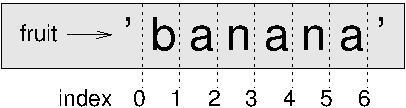
\includegraphics[scale=0.8]{figs/banana.pdf}}
\caption{ดัชนีของแผ่น}
\label{fig.banana}
\end{figure}

ถ้าเราไม่ใส่ดัชนีตัวแรก (ก่อนเครื่องหมายทวิภาค หรือ โคลอน) แผ่นนี้จะเริ่มที่จุดเริ่มต้นของสายอักขระ
ถ้าเราไม่ใส่ดัชนีตัวที่สอง แผนนี้จะยาวไปถึงตอนท้ายของสายอักขระ:

\begin{verbatim}
>>> fruit = 'banana'
>>> fruit[:3]
'ban'
>>> fruit[3:]
'ana'
\end{verbatim}
%
ถ้าดัชนีตัวแรกนั้นมากกว่าหรือเท่ากับตัวที่สอง ผลลัพธ์จะเป็น {\bf สายอักขระว่าง (empty string)}
แทนด้วยเครื่องหมายอัญประกาศสองตัว:
\index{quotation mark}
\index{เครื่องหมายอัญประกาศ}

\begin{verbatim}
>>> fruit = 'banana'
>>> fruit[3:3]
''
\end{verbatim}
%
สายอักขระว่างไม่มีอักขระอยู่เลย และมีความยาวเป็น 0 แต่นอกจากนี้ มันเป็นเหมือนกับสายอักขระอื่น ๆ

มาทำตัวอย่างนี้ต่อ เราคิดว่า {\tt fruit[:]} หมายความว่าอะไร?
ลองดูสิ
\index{copy!slice}
\index{slice!copy}
\index{คัดลอก!ตัดช่วง}
\index{คัดลอก!แผ่น}
\index{ทำสำเนา!ตัดช่วง}
\index{ตัดช่วง!คัดลอก}
\index{ตัดช่วง!ทำสำเนา}



\section{สายอักขระเปลี่ยนแปลงไม่ได้} % (Strings are immutable)}
\index{mutability}
\index{immutability}
\index{string!immutable}
\index{การเปลี่ยนแปลงได้}
\index{การเปลี่ยนแปลงไม่ได้}
\index{สายอักขระ!เปลี่ยนแปลงไม่ได้}

มันน่าลองที่จะใช้ตัวดำเนินการ {\tt []} ในทางซ้ายของคำสั่ง โดยตั้งใจให้เปลี่ยนค่าอักขระในสายอักขระ
เช่น:
\index{TypeError}
\index{exception!TypeError}
\index{ข้อผิดพลาดกับชนิดของค่า}
\index{ข้อยกเว้น!ข้อผิดพลาดกับชนิดของค่า}

\begin{verbatim}
>>> greeting = 'Hello, world!'
>>> greeting[0] = 'J'
TypeError: 'str' object does not support item assignment
\end{verbatim}
%
``object'' ในกรณีนี้คือสายอักขระ และ ``item'' คืออักขระที่เราพยายามจะเปลี่ยนมัน
สำหรับตอนนี้ วัตถุ (object) ก็เหมือนกับค่า แต่เราจะเกลานิยามของคำนี้ทีหลัง (หัวข้อที่~\ref{equivalence}) 
\index{object}
\index{item}
\index{item assignment}
\index{assignment!item}
\index{immutability}
\index{วัตถุ}
\index{รายการ}
\index{การกำหนดค่าให้รายการ}
\index{การกำหนดค่า!รายการ}
\index{การเปลี่ยนแปลงไม่ได้}

เหตุผลของข้อผิดพลาดนี้ คือ สายอักขระนั้น {\bf เปลี่ยนแปลงไม่ได้ (immutable)} ซึ่งหมายความว่า
เราไม่สามารถเปลี่ยนค่าของสายอักขระที่มีอยู่ สิ่งที่ทำได้ดีที่สุดคือเราสามารถสร้างสายอักขระตัวใหม่
ซึ่งเปลี่ยนไปจากสายอักขระเดิม:

\begin{verbatim}
>>> greeting = 'Hello, world!'
>>> new_greeting = 'J' + greeting[1:]
>>> new_greeting
'Jello, world!'
\end{verbatim}
%
ตัวอย่างนี้ทำการเชื่อมอักษรตัวแรกตัวใหม่เข้ากับสไลซ์ของ {\tt greeting} มันไม่มีผลกับ
สายอักขระตัวเดิม
\index{concatenation}
\index{การเชื่อม}


\section{การค้นหา} % (Searching)}
\label{find}

ฟังก์ชันต่อไปนี้ทำอะไร?
\index{find function}
\index{function!find}
\index{ฟังก์ชัน find}
\index{ฟังก์ชัน!find}

\begin{verbatim}
def find(word, letter):
    index = 0
    while index < len(word):
        if word[index] == letter:
            return index
        index = index + 1
    return -1
\end{verbatim}
%
ในมุมหนึ่ง ฟังก์ชัน {\tt find} เป็นส่วนกลับของตัวดำเนินการ {\tt []} 
แทนที่จะรับดัชนีแล้วแยกส่วนอักขระออกมา มันกลับรับอักขระเข้ามา แล้วหาดัชนีที่อักขระตัวนั้นอยู่
ถ้าหาอักขระตัวนั้นไม่พบ ฟังก์ชันคืนค่าเป็น {\tt -1}

นี่คือตัวอย่างแรกที่เราเจอคำสั่ง {\tt return} ที่อยู่ในลูป ถ้า {\tt word[index] == letter}
ฟังก์ชันจะออกจากลูปและคืนค่ากลับไปทันที

ถ้าอักขระนั้นไม่มีในสายอักขระ โปรแกรมจะออกจะลูปแบบปกติ และคืนค่า {\tt -1} กลับไป

รูปแบบของการคำนวณแบบนี้---การแวะผ่านข้อมูลตามลำดับ และคืนค่าเมื่อเราพบสิ่งที่เราหาอยู่---
เรียกว่า {\bf การค้นหา (search)}
\index{traversal}
\index{search pattern}
\index{pattern!search}
\index{การแวะผ่าน}
\index{รูปแบบการค้นหา}
\index{รูปแบบ!การค้นหา}

เพื่อเป็นการฝึกทำ ให้แก้ฟังก์ชัน {\tt find} ให้มีพารามิเตอร์ตัวที่สาม คือ ดัชนีใน 
{\tt word} ตรงที่ให้เริ่มค้นหาค่า


\section{การทำลูปและการนับ} % (Looping and counting)}
\label{counter}
\index{counter}
\index{counting and looping}
\index{looping and counting}
\index{looping!with strings}
\index{ตัวนับ}
\index{การนับและการลูป}
\index{การลูปและการนับ}
\index{การลูป!ด้วยสายอักขระ}

โปรแกรมต่อไปนี้นับว่าอักษร {\tt a} ปรากฏในสายอักขระกี่ครั้ง:

\begin{verbatim}
word = 'banana'
count = 0
for letter in word:
    if letter == 'a':
        count = count + 1
print(count)
\end{verbatim}
%
โปรแกรมนี้สาธิตอีกรูปแบบหนึ่งของการคำนวณที่เรียกว่า {\bf ตัวนับ (counter)}
ตัวแปร {\tt count} มีค่าเริ่มต้นเป็น 0 และจากนั้นเพิ่มทีละหนึ่งในแต่ละครั้งที่เจอ {\tt a}
เมื่อออกจากลูป {\tt count} ก็จะมีค่าผลลัพธ์---จำนวนทั้งหมดของ {\tt a}

\index{encapsulation}
\index{การห่อหุ้ม}
เพื่อเป็นการฝึกทำ ให้หุ้มโค้ดนี้ในฟังก์ชันที่ชื่อว่า {\tt count} และทำให้มันครอบคลุมถึงการ
รับสายอักขระและอักษรเข้ามาเป็นอาร์กิวเมนต์

จากนั้นให้เขียนฟังก์ชันนี้ใหม่ โดยแทนที่จะใช้วิธีแวะผ่านสายอักขระ (string traversing) มันจะใช้ฟังก์ชัน 
{\tt find} เวอร์ชันที่มีพารามิเตอร์สามตัวจากหัวข้อที่แล้ว


\section{เมธอดของสายอักขระ}% (String methods)}
\label{optional}

สายอักขระเตรียมเมธอดสำหรับทำงานที่มีประโยชน์ได้หลากหลาย  เมธอด (method) เหมือนกับฟังก์ชัน---
มันรับอาร์กิวเมนต์และคืนค่ากลับมา---แต่มีกฎวากยสัมพันธ์ที่ต่างออกไป เช่น เมธอด {\tt upper}
รับค่าสายอักขระเข้ามาและคืนค่าเป็นสายอักขระตัวใหม่ที่เป็นอักษรตัวใหญ่ทั้งหมด

\index{method}
\index{string!method}
\index{เมธอด}
\index{สายอักขระ!เมธอด}

แทนที่จะใช้กฎวากยสัมพันธ์ของฟังก์ชัน คือ {\tt upper(word)} มันจะใช้กฎวากยสัมพันธ์ของเมธอด คือ 
{\tt word.upper()}

\begin{verbatim}
>>> word = 'banana'
>>> new_word = word.upper()
>>> new_word
'BANANA'
\end{verbatim}
%
รูปแบบของสัญกรจุด (dot notation) นี้ ระบุชื่อของเมธอด, {\tt upper}, และชื่อของสายอักขระ
ที่จะใช้เมธอดนั้น, {\tt word}  วงเล็บว่างระบุว่าเมธอดนี้ไม่รับอาร์กิวเมนต์เข้ามา
\index{parentheses!empty}
\index{dot notation}
\index{วงเล็บ!ว่าง}
\index{สัญกรณ์จุด}

การเรียกเมธอดนั้นเรียกว่า {\bf การร้องขอ (invocation)}; ในกรณีนี้ เราพูดได้ว่า เรา
ร้องขอให้ทำการ {\tt upper} กับ {\tt word}
\index{invocation}
\index{การร้องขอ}

กลายเป็นว่า มีเมธอดของสายอักขระที่ชื่อว่า {\tt find} ที่เหมือนกันอย่างประหลาดกับฟังก์ชันที่เราได้เขียนไป:

\begin{verbatim}
>>> word = 'banana'
>>> index = word.find('a')
>>> index
1
\end{verbatim}
%
ในตัวอย่างนี้ เราร้องขอให้ทำการ {\tt find} กับ {\tt word} และผ่านอักษรที่เราต้องการหาเข้า
ไปเป็นพารามิเตอร์

ที่จริงแล้ว เมธอด {\tt find} มันครอบคลุมมากกว่าฟังก์ชันของเรา; มันสามารถหา
สายอักขระย่อย (substring) ไม่ใช่แค่อักขระ (character):

\begin{verbatim}
>>> word.find('na')
2
\end{verbatim}
%
โดยปริยาย {\tt find} จะเริ่มที่จุดเริ่มต้นของสายอักขระ แต่มันสามารถรับอาร์กิวเมนต์ตัวที่สอง
คือ ดัชนีที่มันควรจะเริ่มต้นค้นหา:
\index{optional argument}
\index{argument!optional}
\index{อาร์กิวเมนต์ทางเลือก}
\index{อาร์กิวเมนต์!ทางเลือก}

\begin{verbatim}
>>> word.find('na', 3)
4
\end{verbatim}
%
นี่คือตัวอย่างของ {\bf อาร์กิวเมนต์ทางเลือก (optional argument)};
{\tt find} สามารถรับอาร์กิวเมนต์ตัวที่สามได้ด้วย คือ ดัชนีที่มันควรจะหยุดหา:

\begin{verbatim}
>>> name = 'bob'
>>> name.find('b', 1, 2)
-1
\end{verbatim}
%
การค้นหานี้ไม่สำเร็จ เพราะ {\tt b} ไม่ปรากฏอยู่ในช่วงดัชนี {\tt 1} ถึง {\tt 2} โดยไม่รวม {\tt 2}
การค้นหาไปจนถึง, แต่ไม่รวม, ดัชนีตัวที่สองนี้ ทำให้ {\tt find} ทำงานสอดคล้องกันกับตัวดำเนินการเฉือนสายอักขระ (slice)




\section{ตัวดำเนินการ {\tt in}}
\label{inboth}
\index{in operator}
\index{operator!in}
\index{boolean operator}
\index{operator!boolean}
\index{ตัวดำเนินการ in}
\index{ตัวดำเนินการ!in}
\index{ตัวดำเนินการบูลีน}
\index{ตัวดำเนินการ!boolean}

คำว่า {\tt in} เป็นตัวดำเนินการบูลีน ซึ่งรับสายอักขระสองตัว และคืนค่าเป็น {\tt True} ถ้า
ตัวแรกเป็นสายอักขระย่อย (substring) ของตัวที่สอง:

\begin{verbatim}
>>> 'a' in 'banana'
True
>>> 'seed' in 'banana'
False
\end{verbatim}
%
ตัวอย่างเช่น ฟังก์ชันต่อไปนี้พิมพ์อักษรทุกตัวจาก {\tt word1} ที่อยู่ใน {\tt word2}:

\begin{verbatim}
def in_both(word1, word2):
    for letter in word1:
        if letter in word2:
            print(letter)
\end{verbatim}
%
ถ้าเราตั้งชื่อตัวแปรดี ๆ บางครั้งไพธอนจะอ่านเหมือนเป็นภาษาอังกฤษปกติเลย เราอาจจะอ่าน
ลูปนี้ว่า ``for (each) letter in (the first) word, if (the) letter 
(appears) in (the second) word, print (the) letter.'' แปลว่า สำหรับ
letter (อักษรแต่ละตัว) ใน word (คำแรก), ถ้า letter (อักษรตัวนั้น) (ปรากฏอยู่) ใน word 
(อักษรตัวที่สอง) ให้พิมพ์ letter (อักษรตัวนั้น) ออกมา

นี่คือสิ่งที่เราจะได้ถ้าเราเปรียบเทียบคำว่า apples กับ oranges:

\begin{verbatim}
>>> in_both('apples', 'oranges')
a
e
s
\end{verbatim}
%

\section{การเปรียบเทียบสายอักขระ} % (String comparison)}
\index{string!comparison}
\index{comparison!string}
\index{สายอักขระ!การเปรียบเทียบ}
\index{การเปรียบเทียบ!สายอักขระ}

ตัวดำเนินการเชิงสัมพันธ์ทำงานได้กับสายอักขระ เพื่อที่จะหาว่าสายอักขระสองตัวเท่ากันหรือเปล่า:

\begin{verbatim}
if word == 'banana':
    print('All right, bananas.')
\end{verbatim}
%
การดำเนินการเชิงสัมพันธ์แบบอื่นเป็นประโยชน์สำหรับเรียงคำตามลำดับตัวอักษร:

\begin{verbatim}
if word < 'banana':
    print('Your word, ' + word + ', comes before banana.')
elif word > 'banana':
    print('Your word, ' + word + ', comes after banana.')
else:
    print('All right, bananas.')
\end{verbatim}
%
ไพธอนไม่จัดการอักษรตัวใหญ่และตัวเล็กเหมือนกับที่มนุษย์ทำ อักษรตัวใหญ่ทั้งหมดจะอยู่ก่อนอักษร
ตัวเล็กทั้งหมด ดังนั้น:

\begin{verbatim}
Your word, Pineapple, comes before banana.
\end{verbatim}
%
วิธีที่นิยมใช้กันเพื่อที่จะแก้ปัญหานี้ คือการแปลงสายอักขระให้เป็นรูปแบบมาตรฐาน, เช่น แปลง
ให้เป็นตัวเล็กทั้งหมด, ก่อนที่จะเปรียบเทียบ ให้จำอันนี้เอาไว้ในกรณีที่เราจะต้องป้องกัน
ตัวเองจากคนที่ติดอาวุธเป็นสับปะรด (Pineapple)


\section{การดีบัก}
\index{debugging}
\index{traversal}
\index{การดีบัก}
\index{การแวะผ่าน}

เมื่อเราใช้ดัชนีในการแวะผ่านค่าต่าง ๆ ในข้อมูลแบบลำดับ มันยุ่งยากหน่อยที่จะ
เริ่มและจบแบบถูกต้อง นี่คือฟังก์ชันที่ควรจะเปรียบเทียบคำสองคำ และคืนค่า {\tt True}
ถ้าคำหนึ่งเป็นส่วนกลับของอีกคำหนึ่ง แต่มันมีข้อผิดพลาดสองจุด:

\begin{verbatim}
def is_reverse(word1, word2):
    if len(word1) != len(word2):
        return False
    
    i = 0
    j = len(word2)

    while j > 0:
        if word1[i] != word2[j]:
            return False
        i = i+1
        j = j-1

    return True
\end{verbatim}
%
คำสั่ง {\tt if} อันแรกตรวจสอบว่าคำที่รับเข้ามามีความยาวเท่ากันหรือไม่ ถ้าไม่ เรา
สามารถคืนค่า {\tt False} ได้เลย ไม่เช่นนั้น ในการทำงานที่เหลือของฟังก์ชันเราสามารถ
สมมติว่าคำสองคำมีความยาวเท่ากัน นี่คือตัวอย่างของรูปแบบผู้พิทักษ์ (guardian pattern)
ที่กล่าวถึงในหัวข้อที่~\ref{guardian} 
\index{guardian pattern}
\index{pattern!guardian}
\index{index}
\index{รูปแบบผู้พิทักษ์}
\index{รูปแบบ!ผู้พิทักษ์}
\index{ดัชนี}

ตัวแปร {\tt i} และ {\tt j} คือดัชนี:  {\tt i} แวะผ่าน {\tt word1}
จากหน้าไปหลัง ในขณะที่ {\tt j} แวะผ่าน {\tt word2} จากหลังมาหน้า ถ้าเราเจอ
อักษรสองตัวที่ไม่เหมือนกัน เราสามารถคืนค่า {\tt False} กลับไปได้ทันที ถ้าเรา
ทำลูปจนครบรอบแล้วและทุกอักษรเหมือนกัน เราจะคืนค่าเป็น {\tt True}

ถ้าเราทดสอบฟังก์ชันนี้ด้วยคำว่า ``pots'' และ ``stop'' เราคาดว่าจะได้ค่าที่คืนกลับไปเป็น
{\tt True} แต่เรากลับได้ข้อผิดพลาดทางดัชนี (IndexError): 
\index{IndexError}
\index{exception!IndexError}
\index{ข้อผิดพลาดกับดัชนี}
\index{ข้อยกเว้น!ข้อผิดพลาดกับดัชนี}

\begin{verbatim}
>>> is_reverse('pots', 'stop')
...
  File "reverse.py", line 15, in is_reverse
    if word1[i] != word2[j]:
IndexError: string index out of range
\end{verbatim}
%
สำหรับการดีบักข้อผิดพลาดประเภทนี้ สิ่งที่ผมทำอย่างแรก คือ พิมพ์ค่าของดัชนี
ในบรรทัดติดกันที่อยู่ก่อนบรรทัดที่เกิดข้อผิดพลาด

\begin{verbatim}
    while j > 0:
        print(i, j)        # print here
        
        if word1[i] != word2[j]:
            return False
        i = i+1
        j = j-1
\end{verbatim}
%
ตอนนี้ เมื่อผมรันโปรแกรมอีกครั้ง ผมได้ข้อมูลเพิ่มเติม:

\begin{verbatim}
>>> is_reverse('pots', 'stop')
0 4
...
IndexError: string index out of range
\end{verbatim}
%
ครั้งแรกที่เข้าไปในลูป ค่าของ {\tt j} เป็น 4 ซึ่งมันเกินช่วง (out of range)
สำหรับสายอักขระ \verb"'pots'" ดัชนีของอักขระตัวสุดท้ายคือ 3 ดังนั้น 
ค่าเริ่มต้นของ {\tt j} ควรจะเป็น {\tt len(word2)-1}

ถ้าผมแก้ไขข้อผิดพลาดนั้นแล้วรันโปรแกรมอีกที ผมก็จะได้:

\begin{verbatim}
>>> is_reverse('pots', 'stop')
0 3
1 2
2 1
True
\end{verbatim}
%
ครั้งนี้เราได้คำตอบที่ถูกต้อง แต่เหมือนกับว่าลูปทำงานแค่ 3 ครั้ง ซึ่งมันน่าสงสัย เพื่อที่จะได้
มุมมองที่ดีขึ้นว่าเกิดอะไรขึ้น มันเป็นประโยชน์ที่จะวาดแผนภาพสถานะ  ในการวนซ้ำรอบแรก
กรอบของ \verb"is_reverse" ถูกแสดงในรูปที่~\ref{fig.state4}

\index{state diagram} \index{diagram!state}
\index{แผนภาพสถานะ} \index{แผนภาพ!สถานะ}

\begin{figure}
\centerline
{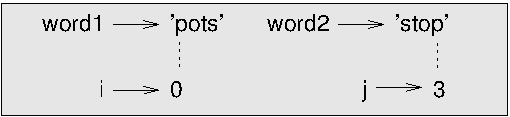
\includegraphics[scale=0.8]{figs/state4.pdf}}
\caption{แผนภาพสถานะ}
\label{fig.state4}
\end{figure}

ผมขออนุญาตจัดเรียงตัวแปรในเฟรมใหม่ และเพิ่มเส้นประเพื่อจะแสดงว่าค่าของ {\tt i} และ
{\tt j} ระบุอักขระใน {\tt word1} และ {\tt word2}

เริ่มด้วยแผนภาพอันนี้ รันโปรแกรมบนกระดาษ แล้วเปลี่ยนค่าของ {\tt i} และ {\tt j}
ในแต่ละรอบของการวนซ้ำ ให้หาข้อผิดพลาดข้อที่สองในฟังก์ชันและแก้มันซะ
\label{isreverse}


\section{อภิธานศัพท์}

\begin{description}

\item[วัตถุ (object):] บางสิ่งที่ตัวแปรสามารถอ้างอิงถึงได้ สำหรับตอนนี้ เราสามารถใช้
``วัตถุ (object)'' and ``ค่า (value)'' สลับกันไปมาได้
\index{object}
\index{วัตถุ}

\item[ลำดับ (sequence):] กลุ่มของค่าที่เรียงไว้ โดยแต่ละค่าถูกระบุได้ด้วยดัชนีที่เป็นจำนวนเต็ม
\index{sequence}
\index{ลำดับ}

\item[รายการ (item):] หนึ่งในค่าที่อยู่ในลำดับ
\index{item}
\index{รายการ}

\item[ดัชนี (index):] จำนวนเต็มที่ใช้เลือกรายการในลำดับ เช่น อักขระในสายอักขระ ในไพธอน
ดัชนีเริ่มต้นที่ 0 
\index{index}
\index{ดัชนี}

\item[แผ่น (slice):] ส่วนของสายอักขระที่ถูกระบุโดยช่วงของดัชนี 
\index{slice}
\index{แผ่น}
\index{ช่วงตัด}
\index{การตัดช่วง}

\item[สายอักขระว่าง (empty string):] สายอักขระที่ไม่มีอักขระอยู่และมีความยาวเป็น 0 ซึ่งเขียนแทนค่าด้วยอัญประกาศสองตัว
\index{empty string}
\index{สายอักขระว่าง}

\item[เปลี่ยนแปลงไม่ได้ (immutable):] คุณสมบัติของลำดับที่ว่ารายการของลำดับนั้นไม่สามารถเปลี่ยนค่าได้ 
\index{immutability}
\index{การเปลี่ยนแปลงไม่ได้}

\item[การแวะผ่าน (traverse):] การวนซ้ำไปในรายการต่าง ๆ ในลำดับ เพื่อดำเนินการอย่างเดียวกันในแต่ละรอบ
\index{traversal}
\index{การแวะผ่าน}

\item[การค้นหา (search):] รูปแบบของการแวะผ่านที่หยุดทำงานเมื่อมันเจอสิ่งที่มันค้นหาแล้ว
\index{search pattern}
\index{pattern!search}
\index{รูปแบบการค้นหา}
\index{รูปแบบ!การค้นหา}

\item[ตัวนับ (counter):] ตัวแปรที่ใช้นับอะไรสักอย่าง โดยปกติแล้วจะมีค่าเริ่มต้นเป็น 0 และถูกเพิ่มค่าขึ้นเรื่อย ๆ
\index{counter}
\index{ตัวนับ}

\item[การร้องขอ (invocation):] คำสั่งที่ใช้เรียกเมธอด
\index{invocation}
\index{การร้องขอ}

\item[อาร์กิวเมนต์ทางเลือก (optional argument):] อาร์กิวเมนต์ของฟังก์ชันหรือเมธอดที่ไม่จำเป็นจะต้องใส่ค่าให้
\index{optional argument}
\index{argument!optional}
\index{อาร์กิวเมนต์ทางเลือก}
\index{อาร์กิวเมนต์!ทางเลือก}

\end{description}


\section{แบบฝึกหัด}

\begin{exercise}
\index{string method}
\index{method!string}
\index{เมธอดของสายอักขระ}
\index{เมธอด!สายอักขระ}

อ่านเอกสารของเมธอดของสายอักขระที่ 
\url{http://docs.python.org/3/library/stdtypes.html#string-methods}
เราอาจจะอยากทดลองกับบางเมธอดเพื่อให้แน่ใจว่าเราเข้าใจว่ามันทำงานยังไง
เมธอด {\tt strip} และ {\tt replace} เป็นเมธอดที่มีประโยชน์เป็นพิเศษ 

เอกสารข้างต้นใช้กฎวากสัมพันธ์ที่อาจจะสับสนหน่อย เช่น ใน \verb"find(sub[, start[, end]])"
วงเล็บทำการระบุอาร์กิวเมนต์ทางเลือก (optional argument) ดังนั้น {\tt sub} 
เป็นสิ่งจำเป็น แต่ {\tt start} เป็นทางเลือก และถ้าเราใส่ {\tt start} เข้าไปแล้ว 
{\tt end} ก็เป็นทางเลือก
\index{optional argument}
\index{argument!optional}
\index{อาร์กิวเมนต์ทางเลือก}
\index{อาร์กิวเมนต์!ทางเลือก}

\end{exercise}


\begin{exercise}
\index{count method}
\index{method!count}
\index{เมธอด count}
\index{เมธอด!count}

มีเมธอดของสายอักขระที่ชื่อว่า {\tt count} ที่ทำงานเหมือนกับฟังก์ชันในหัวข้อที่~\ref{counter}
ให้อ่านเอกสารของเมธอดนี้และเขียนการร้องขอ (invocation) ที่นับจำนวนของ {\tt a}
ในคำว่า \verb"'banana'"
\end{exercise}


\begin{exercise}
\index{step size}
\index{slice operator}
\index{operator!slice}
\index{ขนาดของขั้น}
\index{ตัวดำเนินการเฉือน}
\index{ตัวดำเนินการ!เฉือน}

แผ่นของสายอักขระสามารถรับค่าดัชนีตัวที่สามซึ่งระบุ ``ขนาดของขั้น (step size)'' ได้; นั่นคือ 
จำนวนของที่ว่างระหว่างอักขระที่ติดกัน ขนาดของขั้นเท่ากับ 2 หมายความว่าอักขระเว้นอักขระ;
ส่วน 3 หมายความว่าเอาอักขระมาทุก ๆ 3 ตัว, และอื่น ๆ

\begin{verbatim}
>>> fruit = 'banana'
>>> fruit[0:5:2]
'bnn'
\end{verbatim}

ขนาดของขั้นเท่ากับ -1 จะทำงานกับคำนั้นแบบกลับหลัง ดังนั้น การเฉือน \verb"[::-1]"
ืทำให้เกิดสายอักขระแบบกลับหลัง
\index{palindrome}
\index{พาลินโดรม}

ให้ใช้ลักษณะเฉพาะอันนี้เขียนฟังก์ชัน \verb"is_palindrome" จากแบบฝึกหัดที่~\ref{palindrome} 
ให้เป็นเวอร์ชันที่มี 1 บรรทัด
\end{exercise}


\begin{exercise}

ฟังก์ชันต่อไปนี้ทั้งหมด {\em ตั้งใจ} ที่จะตรวจสอบว่าสายอักขระมีอักษรตัวเล็กหรือไม่ แต่
อย่างน้อยบางฟังก์ชันก็ผิด ในแต่ละฟังก์ชัน ให้บรรยายว่าฟังก์ชันนั้นทำงานอะไรกันแน่
(สมมติว่าพารามิเตอร์ของแต่ละฟังก์ชันเป็นสายอักขระ)

\begin{verbatim}
def any_lowercase1(s):
    for c in s:
        if c.islower():
            return True
        else:
            return False

def any_lowercase2(s):
    for c in s:
        if 'c'.islower():
            return 'True'
        else:
            return 'False'

def any_lowercase3(s):
    for c in s:
        flag = c.islower()
    return flag

def any_lowercase4(s):
    flag = False
    for c in s:
        flag = flag or c.islower()
    return flag

def any_lowercase5(s):
    for c in s:
        if not c.islower():
            return False
    return True
\end{verbatim}

\end{exercise}


\begin{exercise}
\index{letter rotation}
\index{rotation, letter}
\index{การหมุนอักษร}
\index{การหมุน, อักษร}

\label{exrotate}
รหัสซีซาร์ (Caesar cypher) เป็นรูปแบบการเข้ารหัสที่อ่อนแออย่างหนึ่ง ซึ่งเกี่ยวข้องกับการ 
``หมุน'' อักษรแต่ละตัวไปเป็นจำนวนตำแหน่งที่ตายตัว การหมุนอักษรหมายความว่าการเลื่อน
ไปในรายการพยัญชนะ แล้ววนกลับมาพยัญชนะเริ่มต้นหากจำเป็น ดังนั้น การหมุน 'A' ไป 3
ตำแหน่งจะได้ 'D' และการหมุน 'Z' ไป 1 ตำแหน่งจะได้ 'A'

การหมุนคำ เราหมุนอักษรแต่ละตัวในคำในจำนวนที่เท่ากัน เช่น การหมุน ``cheer'' ไป 7
ตำแหน่งจะได้ ``jolly'' และการหมุน ``melon'' ไป -10 ตำแหน่งจะได้ ``cubed''
ในหนังสือ {\em 2001: A Space Odyssey} คอมพิวเตอร์ของยานชื่อว่า HAL ซึ่งเป็นการหมุน
คำว่า IMB ไป -1 ตำแหน่ง 

ตัวอย่างเช่น คำว่า ``sleep'' หมุนไป 9 ตำแหน่ง คือคำว่า ``bunny'' และ
คำว่า ``latex'' หมุนไป 7 ตำแหน่ง คือคำว่า ``shale''

ให้เขียนฟังก์ชันที่ชื่อว่า \verb"rotate_word" ซึ่งรับสายอักขระและจำนวนเต็มเป็นพารามิเตอร์
และคืนค่าเป็นสายอักขระตัวใหม่ที่มีอักษรจากสายอักขระเดิมที่ถูกหมุนเป็นจำนวนที่กำหนดให้

เราอาจจะต้องการใช้ฟังก์ชันพร้อมใช้ {\tt ord} ซึ่งแปลงอักขระเป็นรหัสตัวเลข และ ฟังก์ชัน 
{\tt chr} ซึ่งแปลงรหัสตัวเลขเป็นอักขระ อักษรต่าง ๆ ถูกเข้ารหัสโดยเรียงตามตัวอักษร
ดังนั้น เช่น:

\begin{verbatim}
>>> ord('c') - ord('a')
2
\end{verbatim}

เพราะว่า \verb"'c'" คือ อักษรลำดับที่ 2 ของพยัญชนะ  แต่ระวัง: รหัสตัวเลข
สำหรับอักษรตัวใหญ่นั้นแตกต่างออกไป

(หมายเหตุผู้แปล: อักษรลำดับที่ 0 คือ \verb"'a'")

ตลกที่อาจจะไม่เหมาะสมบนอินเทอร์เน็ตบางครั้งจะถูกเข้ารหัสด้วย ROT13 ซึ่งคือรหัสซีซาร์
ที่หมุนไป 13 ตัว ถ้าเราไม่ได้เป็นคนที่ขุ่นเคืองง่าย ลองหาและถอดรหัสบางอันดู

เฉลย: \url{http://thinkpython2.com/code/rotate.py}.

\end{exercise}



\chapter{กรณีศึกษา เกมทายคำ } %(word play)}
\label{wordplay}

บทนี้นำเสนอกรณีศึกษากรณีที่สอง ซึ่งเกี่ยวกับปริศนาทายคำ โดยการค้นหาคำที่มี
คุณสมบัติตามที่กำหนด เช่น เราจะหาพาลินโดรม (palindrome) ที่ยาวที่สุด
ในภาษาอังกฤษ และหาคำที่มีอักษรในคำเรียงตามลำดับตัวอักษร และผมจะนำเสนอ
แผนการพัฒนาโปรแกรมอีกแบบหนึ่ง: การลดทอนให้เป็นปัญหาที่ถูกแก้ไปแล้ว


\section{การอ่านรายการของคำ}% (Reading word lists)}
\label{wordlist}

สำหรับแบบฝึกหัดในบทนี้ เราต้องการรายการ หรือ ลิสต์ (list) ของคำภาษาอังกฤษ มันมีหลาย
ชุดให้ใช้บนอินเทอร์เน็ต แต่อันที่เหมาะกับจุดประสงค์ของเราคือรายการคำที่จัดเก็บและเผยแพร่สู่
สาธารณะโดย แกรดี้ วอร์ด (Grady Ward) ซึ่งเป็นส่วนหนึ่งของโครงการโมบี้เลซิคอน (Moby lexicon project)
(ดูเพิ่มที่ \url{http://wikipedia.org/wiki/Moby_Project}) มันเป็นรายการที่มี 113,809 
คำที่ใช้เล่นเกมครอสเวิร์ด (crossword) อย่างเป็นทางการ; นั่นคือ คำที่ให้ใช้ได้ในครอสเวิร์ดและ
เกมเกี่ยวกับคำศัพท์อื่น ๆ  ในรายการคำโมบี้นี้มีชื่อไฟล์ว่า {\tt 113809of.fic}; เราสามารถดาวน์โหลด
สำเนาของไฟล์โดยใช้ชื่อที่ง่ายกว่าว่า {\tt words.txt} จาก \url{http://thinkpython2.com/code/words.txt}
\index{Moby Project}
\index{crosswords}
\index{โครงการโมบี้}
\index{ครอสเวิร์ด}

ไฟล์นี้ถูกเก็บอยู่ในรูปแบบตัวข้อความธรรมดา ดังนั้นเราสามารถเปิดมันโดยใช้โปรแกรม
บรรณาธิการข้อความ (text editor) แต่เราก็สามารถอ่านมันจากไพธอนได้ด้วย
ฟังก์ชันพร้อมใช้ {\tt open} รับชื่อของไฟล์เข้ามาเป็นพารามิเตอร์ และคืนค่าเป็น 
{\bf วัตถุไฟล์ (file object)} ที่เราสามารถใช้ในการอ่านไฟล์ได้
\index{open function}
\index{function!open}
\index{plain text}
\index{text!plain}
\index{object!file}
\index{file object}
\index{ฟังก์ชัน open}
\index{ฟังก์ชัน!open}
\index{ข้อความธรรมดา}
\index{ข้อความ!ธรรมดา}
\index{วัตถุ!ไฟล์}
\index{วัตถุไฟล์}

\begin{verbatim}
>>> fin = open('words.txt')
\end{verbatim}
%
{\tt fin} เป็นชื่อที่ใช้โดยทั่วไปสำหรับวัตถุไฟล์ที่ใช้สำหรับอินพุตหรือนำเข้าข้อมูล วัตถุไฟล์มีหลาย
เมธอดสำหรับการอ่าน รวมถึงเมธอด {\tt readline} ซึ่งอ่านอักขระต่าง ๆ จากไฟล์จนกว่าจะเจอ
บรรทัดใหม่ (newline) และคืนค่าเป็นสายอักขระ:
\index{readline method}
\index{method!readline}
\index{เมธอด readline}
\index{เมธอด!readline}

\begin{verbatim}
>>> fin.readline()
'aa\n'
\end{verbatim}
%
คำแรกในลิสต์นี้ คือ ``aa'' ซึ่งแปลว่าลาวาชนิดหนึ่ง ลำดับอักขระ \verb"\n" แทนอักขระ
เริ่มบรรทัดใหม่ (newline character) ซึ่งแบ่งคำนี้จากคำถัดไป

วัตถุไฟล์จดจำว่ามันอ่านถึงไหนแล้วในไฟล์นั้น  ดังนั้น ถ้าเราเรียก {\tt readline} 
อีกครั้งหนึ่ง เราจะได้คำถัดไป:

\begin{verbatim}
>>> fin.readline()
'aah\n'
\end{verbatim}
% 
คำถัดไป คือคำว่า ``aah'' ซึ่งเป็นคำที่แท้จริง ดังนั้น หยุดมองผมแบบนั้นซะที
หรือ ถ้ามันเป็นอักขระเริ่มบรรทัดใหม่ที่ทำให้ขัดใจ เราสามารถกำจัดมันด้วยเมธอด
ของสายอักขระที่ชื่อว่า {\tt strip}:
\index{strip method}
\index{method!strip}
\index{เมธอด strip}
\index{เมธอด!strip}

\begin{verbatim}
>>> line = fin.readline()
>>> word = line.strip()
>>> word
'aahed'
\end{verbatim}
%
เราสามารถใช้วัตถุไฟล์เป็นส่วนหนึ่งของลูป {\tt for} ได้ โปรแกรมนี้อ่านไฟล์ {\tt words.txt}
และพิมพ์แต่ละคำออกมาคำละบรรทัด:
\index{open function}
\index{function!open}
\index{ฟังก์ชัน open}
\index{ฟังก์ชัน!open}

\begin{verbatim}
fin = open('words.txt')
for line in fin:
    word = line.strip()
    print(word)
\end{verbatim}
%

\section{แบบฝึกหัด}

เฉลยสำหรับแบบฝึกหัดต่อไปนี้จะอยู่ในหัวข้อถัดไป อย่างน้อยเราควรพยายามที่จะทำแต่ละข้อ
ก่อนที่จะไปดูเฉลย

\begin{exercise}
ให้เขียนโปรแกรมซึ่งอ่านไฟล์ {\tt words.txt} และพิมพ์คำที่มีความยาวมากกว่า
20 อักขระ (ไม่นับเว้นวรรค)
\index{whitespace}
\index{เว้นวรรค}

\end{exercise}

\begin{exercise}

ในปี ค.ศ. 1939 เอิร์นเนิสต์ วินเซนต์ ไรต์ (Ernest Vincent Wright) ได้ตีพิมพ์ นวนิยาย
ความยาว 50,000 คำที่ชื่อว่า {\em แกดสบี้ (Gadsby)} ซึ่งไม่มีอักษร ``e'' อยู่เลย
เนื่องจาก ``e'' เป็นอักษรที่นิยมใช้เป็นปกติในภาษาอังกฤษ มันจึงไม่ง่ายเลยที่จะทำแบบนั้น

ที่จริงแล้ว มันยากที่จะสร้างความคิดโดดเดี่ยวโดยปราศจากสัญลักษณ์ที่นิยมใช้อันนี้ การทำเป็นไป
อย่างเชื่องช้าในตอนแรก แต่ด้วยความรอบคอบและการฝึกฝนอันยาวนาน เราสามารถค่อย ๆ เพิ่ม
ความง่ายขึ้น

เอาเถอะ ผมจะหยุดตรงนี้

ให้เขียนฟังก์ชันที่ชื่อว่า \verb"has_no_e" ที่คืนค่า {\tt True} ถ้าคำที่กำหนดให้ไม่มีอักษร
``e'' ในคำนั้น

ให้แก้ไขโปรแกรมจากหัวข้อที่แล้วให้พิมพ์แค่คำที่ไม่มี ``e'' และคำนวณเปอร์เซนต์ของคำในรายการ
ที่ไม่มี ``e''
\index{lipogram}
\index{ไลโปแกรม}

\end{exercise}


\begin{exercise} 

ให้เขียนฟังก์ชันที่ชื่อว่า {\tt avoids} ซึ่งรับคำหนึ่งคำ และสายอักขระของอักษรต้องห้าม และ
ึิคืนค่า {\tt True} ถ้าคำนั้นไม่มีอักษรต้องห้ามที่กำหนดให้เลย

ให้แก้ไขโปรแกรมเพื่อรับสายอักขระของอักษรต้องห้ามจากผู้ใช้ และจากนั้นพิมพ์จำนวน
คำที่ไม่มีอักษรต้องห้ามใด ๆ เลย

เราสามารถหาการรวมกันของอักษรต้องห้าม 5 ตัว ที่แยกคำออกไปเป็นจำนวนน้อยที่สุดออกไปได้หรือไม่?

\end{exercise}



\begin{exercise}

ให้เขียนฟังก์ชันที่ชื่อว่า \verb"uses_only" ซึ่งรับคำหนึ่งคำ และสายอักขระของอักษร และ
คืนค่าเป็น {\tt True} ถ้าคำนั้นมีแค่อักษรในลิสต์ที่กำหนดให้  เราสามารถสร้างประโยคโดย
ใช้แค่อักษรใน {\tt acefhlo} ได้หรือไม่? แล้วที่ไม่ใช่คำว่า ``Hoe alfalfa'' ล่ะ?

\end{exercise}


\begin{exercise} 

ให้เขียนฟังก์ชันที่ชื่อว่า \verb"uses_all" ที่รับคำหนึ่งคำ และสายอักขระของอักษรบังคับ (ที่ต้องใช้)
และให้คืนค่าเป็น {\tt True} ถ้าคำนั้นใช้อักษรบังคับอย่างน้อยตัวละหนึ่งครั้ง  มีคำกี่คำที่ใช้
สระทั้งหมดใน {\tt aeiou}? แล้วใน {\tt aeiouy} ล่ะ?

\end{exercise}


\begin{exercise}

ให้เขียนฟังก์ชันชื่อว่า \verb"is_abecedarian" ซึ่งคืนค่าเป็น {\tt True} ถ้าอักษรในคำ
นั้นปรากฏตามลำดับตัวอักษร (ใช้อักษรคู่ได้)
มีคำที่เป็น เอบีซีดาเรียน (abecedarian) ทั้งหมดกี่คำ?
\index{abecedarian}
\index{เอบีซีดาเรียน}

\end{exercise}



\section{การค้นหา} % (Search)}
\label{search}
\index{search pattern}
\index{pattern!search}
\index{รูปแบบการค้นหา}
\index{รูปแบบ!การค้นหา}

แบบฝึกหัดทั้งหมดในหัวข้อที่แล้วมีบางอย่างที่เหมือนกัน: มันสามารถแก้ได้โดยใช้
รูปแบบการค้นหาที่เราเจอในหัวข้อที่~\ref{find} ตัวอย่างที่ง่ายที่สุดคือ:


\begin{verbatim}
def has_no_e(word):
    for letter in word:
        if letter == 'e':
            return False
    return True
\end{verbatim}
%
ลูป {\tt for} แวะผ่านอักขระใน {\tt word} ถ้าเราเจออักษร ``e'' เราสามารถคืนค่า {\tt False};
ได้ทันที ไม่เช่นนั้น เราต้องไปที่อักษรตัวถัดไป  ถ้าเราออกจากลูปแบบปกติแล้ว นั่นหมายความว่า
เราไม่เจอ ``e'' ดังนั้น เราสามารถคืนค่า {\tt True} ได้
\index{traversal}
\index{การแวะผ่าน}

\index{in operator}
\index{operator!in}
\index{ตัวดำเนินการ in}
\index{ตัวดำเนินการ!in}

เราอาจจะเขียนฟังก์ชันนี้ให้กระชับขึ้นโดยการใช้ตัวดำเนินการ {\tt in} แต่ผมเริ่มจาก
เวอร์ชันนี้เพราะมันสาธิตตรรกะของรูปแบบการค้นหา

\index{generalization}
\index{การทำให้ครอบคลุม}
ฟังก์ชัน {\tt avoids} มันครอบคลุมมากกว่าเวอร์ชันของ \verb"has_no_e" แต่มัน
มีโครงสร้างที่เหมือนกัน:

\begin{verbatim}
def avoids(word, forbidden):
    for letter in word:
        if letter in forbidden:
            return False
    return True
\end{verbatim}
%
เราสามารถคืนค่า {\tt False} ทันทีที่เราเจออักษรต้องห้าม; ถ้าเราไปถึงการจบลูปแล้ว
เราก็คืนค่า {\tt True} กลับไป

ฟังก์ชัน \verb"uses_only" ก็เหมือนกัน ยกเว้นว่าความหมายของเงื่อนไขก็จะกลับกัน: 

\begin{verbatim}
def uses_only(word, available):
    for letter in word: 
        if letter not in available:
            return False
    return True
\end{verbatim}
%
แทนที่จะใช้รายการของอักษรต้องห้าม เรามีรายการของอักษรที่ใช้ได้ ถ้าเราเจออักษรใน 
{\tt word} ที่ไม่ได้อยู่ใน {\tt available} เราสามารถคืนค่า {\tt False} 
กลับไปได้

ฟังก์ชัน \verb"uses_all" ก็เหมือนกัน ยกเว้นว่าเรากลับหน้าที่ของคำและสายอักขระ
ของอักษร:

\begin{verbatim}
def uses_all(word, required):
    for letter in required: 
        if letter not in word:
            return False
    return True
\end{verbatim}
%
แทนที่จะแวะผ่านอักษรต่าง ๆ ใน {\tt word} ลูปนี้แวะผ่านอักษรบังคับเท่านั้น ถ้าอักษรบังคับ
ตัวไหนไม่ปรากฏในคำ เราสามารถคืนค่าเป็น {\tt False} ได้
\index{traversal}
\index{การแวะผ่าน}

ถ้าเราคิดจริงจังเหมือนกับนักวิทยาการคอมพิวเตอร์ เราจะรู้จำได้ว่า \verb"uses_all"
เป็นกรณีตัวอย่างของปัญหาที่ถูกแก้ไปแล้ว และเราก็จะเขียนว่า:

\begin{verbatim}
def uses_all(word, required):
    return uses_only(required, word)
\end{verbatim}
%
นี่คือตัวอย่างของแผนการพัฒนาโปรแกรมที่เรียกว่า {\bf การลดทอนให้เป็นปัญหาที่ถูกแก้ไปแล้ว}
ซึ่งหมายความว่าเรารู้จำว่าปัญหาที่เรากำลังแก้อยู่นี้เป็นกรณีตัวอย่างของปัญหาที่เคยถูกแก้ไปแล้ว
แล้วเราก็ประยุกต์ใช้ทางแก้ปัญหาที่มันมีอยู่แล้ว
\index{development plan!reduction}
\index{แผนการพัฒนา!การลดทอน}



\section{ลูปด้วยดัชนี} % (Looping with indices)}
\index{looping!with indices}
\index{index!looping with}
\index{ลูป!ด้วยดัชนี}
\index{ดัชนี!ลูปด้วย}

ผมเขียนฟังก์ชันในหัวข้อที่แล้วด้วยลูป {\tt for} เพราะผมแค่ต้องการอักขระในสายอักขระ;
ผมไม่ได้ต้องการที่จะทำอะไรกับดัชนี

สำหรับฟังก์ชัน \verb"is_abecedarian" เราต้องเปรียบเทียบอักษรที่อยู่ติดกัน ซึ่งจะยุ่งยากหน่อย
เมื่อใช้ลูป {\tt for}:

\begin{verbatim}
def is_abecedarian(word):
    previous = word[0]
    for c in word:
        if c < previous:
            return False
        previous = c
    return True
\end{verbatim}

ทางเลือกหนึ่งคือการใช้การเรียกซ้ำ (recursion):

\begin{verbatim}
def is_abecedarian(word):
    if len(word) <= 1:
        return True
    if word[0] > word[1]:
        return False
    return is_abecedarian(word[1:])
\end{verbatim}

อีกทางหนึ่งคือการใช้ลูป {\tt while}:

\begin{verbatim}
def is_abecedarian(word):
    i = 0
    while i < len(word)-1:
        if word[i+1] < word[i]:
            return False
        i = i+1
    return True
\end{verbatim}
%
ลูปเริ่มที่ {\tt i=0} และจบเมื่อ {\tt i=len(word)-1} ในแต่ละครั้งที่รันลูป มันจะเปรียบเทียบ
อักขระตัวที่ $i$th (ซึ่งเราสามารถคิดว่ามันเป็นอักขระตัวปัจจุบันได้) กับอักขระตัวที่ $i+1$th
(ซึ่งเราสามารถคิดว่ามันเป็นอักขระตัวถัดไป)

ถ้าอักขระตัวถัดไปน้อยกว่า (มาก่อนตามลำดับตัวอักษร) ตัวปัจจุบันแล้ว เราค้นพบตัวทำลาย
แนวโน้มการเป็น abecedarian และเราจะคืนค่าเป็น {\tt False}

ถ้าเราไปถึงตอนท้ายของลูปโดยไม่เจออะไรผิดพลาดแล้ว คำนั้นก็ผ่านการทดสอบ ในการโน้มน้าว
ตัวเราเองว่าลูปนั้นจบแบบถูกต้อง ให้พิจารณาตัวอย่างเช่นคำว่า \verb"'flossy'" ความยาวของคำคือ 5
ดังนั้น ครั้งสุดท้ายที่ลูปทำงานคือเมื่อ {\tt i} is 4 ซึ่งเป็นดัชนีของอักขระตัวรองสุดท้าย
ในการวนซ้ำรอบสุดท้าย มันเปรียบเทียบอักขระตัวรองสุดท้ายนี้กับอักขระตัวสุดท้าย ซึ่งเป็นสิ่งที่
เราต้องการ

\index{palindrome}
\index{พาลินโดรม}

นี่คือเวอร์ชันของฟังก์ชัน \verb"is_palindrome" (ไปดูแบบฝึกหัดที่~\ref{palindrome}) ซึ่ง
ใช้ดัชนีสองตัว; ตัวแรกเริ่มที่จุดเริ่มต้นและนับขึ้นไปในคำ; อีกตัวเริ่มที่ตอนจบแล้วนับถอยหลังลงมา

\begin{verbatim}
def is_palindrome(word):
    i = 0
    j = len(word)-1

    while i<j:
        if word[i] != word[j]:
            return False
        i = i+1
        j = j-1

    return True
\end{verbatim}

หรือเราสามารถจะลดทอนให้เป็นปัญหาที่ถูกแก้ไปแล้ว และเขียนว่า:
\index{reduction to a previously solved problem}
\index{development plan!reduction}
\index{การลดทอนให้เป็นปัญหาที่ถูกแก้ไปแล้ว}
\index{แผนการพัฒนา!การลดทอน}

\begin{verbatim}
def is_palindrome(word):
    return is_reverse(word, word)
\end{verbatim}
%
โดยการใช้ฟังก์ชัน \verb"is_reverse" จากหัวข้อที่~\ref{isreverse}


\section{การดีบัก}
\index{debugging}
\index{testing!is hard}
\index{program testing}
\index{การดีบัก}
\index{การทดสอบ!ยาก}
\index{การทดสอบโปรแกรม}

การทดสอบโปรแกรมนั้นยาก ฟังก์ชันต่าง ๆ ในบทนี้มันค่อนข้างง่ายที่จะทดสอบ เพราะว่าเรา
สามารถตรวจสอบผลลัพธ์โดยมือได้ ถึงกระนั้น มันก็ยังถือว่าอยู่ระหว่างความยากและเป็นไปไม่ได้ที่จะเลือก
ชุดของคำเพื่อทดสอบหาข้อผิดพลาดที่สามารถเกิดขึ้นได้ทั้งหมด

เอาฟังก์ชัน \verb"has_no_e" เป็นตัวอย่าง มีสองกรณีที่ชัดเจนที่จะตรวจสอบ: คำที่มี `e' จะต้อง
คืนค่ากลับมาเป็น {\tt False} และคำที่ไม่มีควรจะคืนค่ากลับมาเป็น {\tt True} เราควรจะไม่มีปัญหา
ในการคิดคำหนึ่งคำในแต่ละกรณี

ในแต่ละกรณี มีกรณีย่อยบางอันที่ไม่ค่อยชัดเจนเท่า เราควรจะทดสอบด้วยคำที่มี ``e'' ตอนขึ้นต้น,
ลงท้าย และตรงกลาง ๆ คำ เราควรทดสอบด้วยคำยาว คำสั้น และคำสั้นมาก ๆ เช่น สายอักขระว่าง
สายอักขระว่างเป็นตัวอย่างของ {\bf กรณีพิเศษ} ซึ่งเป็นหนึ่งในกรณีที่ไม่ค่อยชัดเจนที่มีข้อผิดพลาด
เกิดขึ้นบ่อย ๆ
\index{special case}
\index{กรณีพิเศษ}

นอกจากการทดสอบกรณีที่เราเป็นคนสร้างขึ้นมาแล้ว เราสามารถทดสอบโปรแกรมของเรา
ด้วยรายการคำศัพท์ เช่น {\tt words.txt} อีกด้วย ในการตรวจเอ้าต์พุต เราอาจจะ
สามารถจับข้อผิดพลาดได้  แต่ให้ระวัง: เราอาจจะจับข้อผิดพลาดประเภทหนึ่ง (คำที่ไม่ควรจะ
มีในเอ้าต์พุต แต่ดันมี) และ ไม่สามารถจับอีกประเภทหนึ่งได้ (คำที่ควรจะมีในเอ้าต์พุต แต่ดันไม่มี)

โดยทั่วไปแล้ว การทดสอบสามารถช่วยเราหาบัก (bug) ได้ แต่มันไม่ง่ายที่จะสร้างชุดทดสอบที่ดี
และแม้กระทั่งถึงเราสร้างได้ เราอาจจะไม่สามารถแน่ใจได้ว่าโปรแกรมเราถูกต้องอย่างหมดจดหรือไม่
ตามที่นักวิทยาการคอมพิวเตอร์ในตำนานได้กล่าวไว้:
\index{testing!and absence of bugs}
\index{การทดสอบ!และการไม่มีบัก}

\begin{quote}
การทดสอบโปรแกรมสามารถใช้เพื่อแสดงว่ามีบัก
แต่มันไม่สามารถแสดงได้ว่าไม่มีบัก!

--- เอ็ดสเกอร์ ไดก์สตรา (Edsger W. Dijkstra)
\end{quote}
\index{Dijkstra, Edsger}


\section{อภิธานศัพท์}

\begin{description}

\item[วัตถุไฟล์ (file object):] ค่าที่ใช้แทนไฟล์ที่ถูกเปิดใช้งาน
\index{file object}
\index{object!file}
\index{วัตถุไฟล์}
\index{วัตถุ!ไฟล์}

\item[ลดทอนให้เป็นปัญหาที่ถูกแก้ไปแล้ว (reduction to a previously solved problem):] 
วิธีการแก้ปัญหาโดยการทำให้อยู่ในรูปแบบของปัญหาที่เคยถูกแก้ไปแล้ว   
\index{reduction to a previously solved problem}
\index{development plan!reduction}
\index{การลดทอนให้เป็นปัญหาที่ถูกแก้ไปแล้ว}
\index{แผนการพัฒนา!การลดทอน}

\item[กรณีพิเศษ (special case):] กรณีทดสอบที่ไม่ปกติ หรือไม่ชัดแจ้ง (และไม่น่าจะถูกจัดการได้อย่างถูกต้อง)
\index{special case}
\index{กรณีพิเศษ}

\end{description}


\section{แบบฝึกหัด}

\begin{exercise}
\index{Car Talk}
\index{Puzzler}
\index{double letters}
\index{รายการคาร์ทอล์ก}
\index{ปริศนา}
\index{อักษรคู่}

คำถามนี้มาจากปริศนาในวิทยุรายการ {\em Car Talk} (\url{http://www.cartalk.com/content/puzzlers}):

\begin{quote}
จงหาคำมาหนึ่งคำที่มีอักษรคู่สามคู่ติดกัน ผมจะให้สองสามคำที่เกือบจะเป็น แต่ไม่ได้เป็น เช่น
คำว่า committee, c-o-m-m-i-t-t-e-e มันจะเยี่ยมเลยยกเว้นดันมี `i' ที่แอบเข้าไปอยู่ในคำ
หรือคำว่า Mississippi: M-i-s-s-i-s-s-i-p-p-i ถ้าเราสามารถเอา i ออกมาได้ ก็จะใช้ได้
แต่มีอีกคำที่มีอักษรคู่สามคู่ติดกัน และเท่าที่ผมรู้ มันอาจจะเป็นคำเดียวด้วยซ้ำ แน่นอนว่ามันอาจจะมี
500 คำอื่น แต่ผมสามารถคิดได้แค่คำเดียว คำนั้นคือคำว่าอะไร?
\end{quote}

จงเขียนโปรแกรมเพื่อหาคำนั้น
เฉลย: \url{http://thinkpython2.com/code/cartalk1.py}.

\end{exercise}


\begin{exercise}
นี่คือปริศนาอีกข้อจากรายการ {\em Car Talk} (\url{http://www.cartalk.com/content/puzzlers}):
\index{Car Talk}
\index{Puzzler}
\index{odometer}
\index{palindrome}
\index{รายการคาร์ทอล์ก}
\index{ปริศนา}
\index{เครื่องวัดระยะ}
\index{พาลินโดรม}

\begin{quote}
``ผมขับรถบนทางหลวงเมื่อวันก่อน และบังเอิญสังเกตเครื่องวัดระยะทาง เหมือนเครื่องวัด
ระยะทางส่วนมาก มันแสดงเลขหกหลักเป็นจำนวนไมล์ถ้วน ๆ เท่านั้น ดังนั้น ถ้ารถของ
ผมเดินทางมาแล้ว 300000 ไมล์ ผมก็จะเห็นเลข 3-0-0-0-0-0 เป็นต้น

``คราวนี้นะ สิ่งที่ผมเห็นมันน่าสนใจมาก ผมสังเกตว่าเลขสี่ตัวสุดท้ายเป็นแบบพาลินโดรม (palindromic);
นั่นคือ มันเป็นเลขตัวเดียวกันทั้งไปหน้าแล้วกลับหลัง เช่น 5-4-4-5 เป็นพาลินโดรม ดังนั้น เครื่องวัดระยะ
ทางของผมอาจจะขึ้นว่า 3-1-5-4-4-5

``อีกหนึ่งไมล์ต่อมา เลขห้าตัวสุดท้ายก็เป็นแบบพาลินโดรม เช่น มันอาจจะเป็น 3-6-5-4-5-6
และอีกหนึ่งไมล์หลังจากนั้น เลขสี่ตัวตรงกลางก็เป็นแบบพาลินโดรม 
คุณพร้อมแล้วใช่ไหม?
อีกหนึ่งไมล์ต่อมา เลขทั้งหกตัวก็เป็นแบบพาลินโดรม! 

``คำถามคือ เลขตัวแรกที่ผมสังเกตเห็น คือเลขอะไร?''
\end{quote}

ให้เขียนโปรแกรมไพธอนที่ทดสอบเลขที่มีหกหลักทั้งหมด และพิมพ์เลขที่ตรงกับสิ่งที่กำหนดข้างต้น
ออกมา
เฉลย: \url{http://thinkpython2.com/code/cartalk2.py}.

\end{exercise}


\begin{exercise}
นี่ก็เป็นปริศนาอีกข้อจากรายการ {\em Car Talk} ที่เราสามารถแก้ได้ด้วยการค้นหา
(\url{http://www.cartalk.com/content/puzzlers}):
\index{Car Talk}
\index{Puzzler}
\index{palindrome}
\index{รายการคาร์ทอล์ก}
\index{ปริศนา}
\index{พาลินโดรม}

\begin{quote}
``เร็ว ๆ นี้ ผมได้ไปเยี่ยมแม่ของผม และเราพบว่าเลขสองหลักที่เป็นอายุของผมนั้นเมื่ออ่านย้อนกลับ
แล้วจะเป็นอายุของแม่ เช่น ถ้าแม่อายุ 73 ผมจะอายุ 37 เราสงสัยว่าสิ่งนี้มันเกิดขึ้นบ่อยขนาดไหน
ในปีที่ผ่าน ๆ มา แต่เราก็ออกทะเลไปคุยเรื่องอื่น และก็ไม่ได้คิดหาคำตอบ

``เมื่อผมกลับถึงบ้าน ผมก็พบว่าเลขของอายุของพวกเรานั้นกลับกันมาหกครั้งแล้ว ผมยังพบว่าถ้าเราโชคดี
มันจะเกิดขึ้นอีกครั้งในอีกไม่กี่ปีนี้ และถ้าเราโชคดีมาก ๆ มันก็จะเกิดขึ้นอีกครั้งหลักจากนั้น ดังนั้น
คำถามคือ ตอนนี้ผมอายุเท่าไหร่กันนะ''

\end{quote}

ให้เขียนโปรแกรมไพธอนที่ค้นหาคำตอบแก่ปริศนานี้ 
คำใบ้: เราอาจจะพบว่า เมธอดของสายอักขระที่ชื่อว่า {\tt zfill} นั้นเป็นประโยชน์

เฉลย: \url{http://thinkpython2.com/code/cartalk3.py}.

\end{exercise}



\chapter{ลิสต์}

บทนี้เป็นเรื่องของชนิดข้อมูล ชนิดหนึ่งที่มีประโยชน์มากที่สุดในภาษาไพธอน
นั่นคือ ลิสต์ (list).
เราจะเรียนเพิ่มเติมในเรื่อง\textit{ออบเจ๊คต์} (\textit{object})
และสิ่งที่จะเกิดขึ้น ถ้าเรามีมากกว่าหนึ่งชื่อสำหรับ\textit{ออบเจ๊คต์}เดียวกัน.
%You will also learn more about objects and what can happen when you have
%more than one name for the same object.


\section{ลิสต์เป็นชุดลำดับ}
\label{sequence}

ในลักษณะเดียวกับสายอักขระ (string),
ลิสต์เป็นลำดับของค่าต่าง ๆ.
ในสายอักขระ ค่าต่าง ๆ ที่ว่า คือ ตัวอักษร.
ในลิสต์ ค่าต่าง ๆ นั้นอาจจะเป็นอะไรก็ได้.
ค่าต่าง ๆ ในลิสต์นั้น จะเรียกว่า \textbf{อิลิเมนต์} (\textbf{elements})
หรือบางครั้งก็เรียกว่า \textbf{ไอเท็ม} (\textbf{items}).
\index{list}
\index{type!list}
\index{element}
\index{sequence}
\index{item}
\index{ลิสต์}
\index{ชนิดข้อมูล!ลิสต์}
\index{อิลิเมนต์}
\index{ชุดลำดับ}
\index{ไอเท็ม}

มีหลายวิธีที่ใช้สร้างลิสต์ได้
วิธีที่ง่ายที่สุดคือ ล้อมอิลิเมนต์ต่าง ๆ ไว้ในวงเล็มสี่เหลี่ยม
(\verb"[" และ \verb"]") เช่น

\begin{verbatim}
[10, 20, 30, 40]
['crunchy frog', 'ram bladder', 'lark vomit']
\end{verbatim}
%
ตัวอย่างแรก เป็นลิสต์ของเลขจำนวนเต็มสี่ตัว.
ตัวอย่างที่สอง เป็นลิสต์ของสายอักขระสามตัว.
อิลิเมนต์ต่าง ๆ ในลิสต์ไม่จำเป็นต้องเป็นชนิดเดียวกัน.
ลิสต์ข้างล่างนี้ มีสายอักขระ เลขทศนิยม เลขจำนวนเต็ม และลิสต์อีกอัน

\begin{verbatim}
['spam', 2.0, 5, [10, 20]]
\end{verbatim}
%
ลิสต์ที่อยู่ในอีกลิสต์หนึ่ง จะเรียกว่า \textbf{ลิสต์ซ้อนใน} (\textbf{nested list}).
\index{nested list}
\index{list!nested}
\index{ลิสต์ซ้อนใน}
\index{ลิสต์!ซ้อนใน}

ลิสต์ที่ไม่มีอิลิเมนต์อยู่เลย จะเรียกว่า ลิสต์ว่าง (empty list).
เราสามารถสร้างลิสต์ว่างได้ด้วยวงเล็บสี่เหลี่ยมว่าง ๆ \verb"[]".
\index{empty list}
\index{list!empty}
\index{ลิสต์ว่าง}
\index{ลิสต์!ว่าง}

ซึ่งก็น่าจะเดาได้ว่า เราสามารถกำหนดค่าที่เป็นลิสต์ให้กับตัวแปรได้

\begin{verbatim}
>>> cheeses = ['Cheddar', 'Edam', 'Gouda']
>>> numbers = [42, 123]
>>> empty = []
>>> print(cheeses, numbers, empty)
['Cheddar', 'Edam', 'Gouda'] [42, 123] []
\end{verbatim}
%
\index{assignment}
\index{การกำหนดค่า}

\section{ลิสต์เป็นชนิดข้อมูลที่เปลี่ยนแปลงได้}
\label{mutable}
\index{list!element}
\index{access}
\index{index}
\index{bracket operator}
\index{operator!bracket}
\index{ลิสต์!อิลิเมนต์}
\index{ตัวดำเนินการวงเล็บสี่เหลี่ยม}

วิธีการเข้าถึงอิลิเมนต์ของลิสต์คล้ายกับ
วิธีการเข้าถึงตัวอักษรในสายอักขระ
นั่นคือ ใช้ตัวดำเนินการวงเล็บสี่เหลี่ยม.
นิพจน์ภายในวงเล็บสี่เหลี่ยมจะระบุ\textit{ดัชนี}(\textit{index} หรือเลขลำดับ)ของอิลิเมนต์
ทบทวนว่า ดัชนีแรกเริ่มต้นที่ 0.

จากตัวอย่างที่แล้ว
\begin{verbatim}
>>> cheeses[0]
'Cheddar'
\end{verbatim}
%
สิ่งที่ต่างจาก\textit{สายอักขระ}(\textit{string}) 
ก็คือ ลิสต์เป็นชนิดข้อมูลที่เปลี่ยนแปลงได้ (mutable).
ถ้าตัวดำเนินการวงเล็บสี่เหลี่ยมอยู่ทางซ้ายมือของ\textit{การกำหนดค่า}(\textit{assignment})
มันจะระบุอิลิเมนต์ของลิสต์ที่จะกำหนดค่าให้ใหม่.
\index{mutability}
\index{ความสามารถในการเปลี่ยนแปลงได้}

\begin{verbatim}
>>> numbers = [42, 123]
>>> numbers[1] = 5
>>> numbers
[42, 5]
\end{verbatim}
%
อิลิเมนต์ดัชนี 1 ของตัวแปร \texttt{numbers}
ที่เคยเป็น 123 ตอนนี้กลายเป็น 5.
\index{index!starting at zero}
\index{zero, index starting at}
\index{ดัชนี!เริ่มที่ศูนย์}

รูป~\ref{fig.liststate} 
แสดง\textit{แผนภาพสถานะ}(\textit{state diagram})
ของตัวแปร \texttt{cheeses}, 
\texttt{numbers} 
และ \texttt{empty}.
\index{state diagram}
\index{diagram!state}
\index{แผนภาพสถานะ}
%
ลิสต์แสดงเป็นกล่องที่มีคำว่า ``list'' กำกับอยู่ข้างบน
และมีอิลิเมนต์ต่าง ๆ อยู่ภายใน.
ตัวแปร \texttt{cheeses} อ้างถึงลิสต์ที่มีสามอิลิเมนต์ ใช้ดัชนี 0, 1, และ 2.
ตัวแปร \texttt{numbers} มีสองอิลิเมนต์.
แผนภาพแสดงค่าของอิลิเมนต์ที่สอง (ดัชนี 1) ถูกเปลี่ยนจาก 123 เป็น 5.
ตัวแปร \texttt{empty} อ้างถึงลิสต์ที่ไม่มีอิลิเมนต์.
\index{item assignment}
\index{assignment!item}
\index{reassignment}
\index{การกำหนดค่าอิลิเมนต์}

\begin{figure}
\centerline
{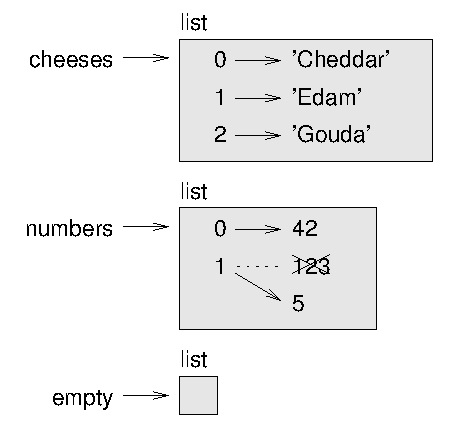
\includegraphics[scale=0.8]{figs/liststate.pdf}}
\caption{แผนภาพสถานะ.}
\label{fig.liststate}
\end{figure}

ดัชนีของลิสต์ทำงานแบบเดียวกับดัชนีของสายอักขระ

\begin{itemize}

\item นิพจน์ที่ให้ผลเป็นจำนวนเต็มใด ๆ สามารถใช้เป็นดัชนีได้
เช่น
\begin{verbatim}
>>> cheeses[3 - 2]
'Edam'
\end{verbatim}

\item ถ้าเราพยายามไปอ่านหรือเขียนอิลิเมนต์ที่ไม่มีอยู่
เราจะได้ \texttt{IndexError} ออกมา เช่น
\index{exception!IndexError}
\index{IndexError}
\begin{verbatim}
>>> cheeses[3]
Traceback (most recent call last):
  File "<stdin>", line 1, in <module>
IndexError: list index out of range
\end{verbatim}

\item ถ้าดัชนีเป็นเลขลบ
มันจะนับย้อนกลับจากอิลิเมนต์สุดท้ายในลิสต์ เช่น
\begin{verbatim}
>>> cheeses[-1]
'Gouda'
\end{verbatim}

\end{itemize}
\index{list!index}
\index{ลิสต์!ดัชนี}

\index{list!membership}
\index{membership!list}
\index{in operator}
\index{operator!in}
\index{ลิสต์!สมาชิก}
\index{ตัวดำเนินการ!in}

ตัวดำเนินการ \texttt{in} ก็ทำงานกับลิสต์ได้เหมือนกับในสายอักขระ.

\begin{verbatim}
>>> cheeses = ['Cheddar', 'Edam', 'Gouda']
>>> 'Edam' in cheeses
True
>>> 'Brie' in cheeses
False
\end{verbatim}

\section{การท่องสำรวจลิสต์}
\index{list!traversal}
\index{traversal!list}
\index{for loop}
\index{loop!for}
\index{statement!for}
\index{ลิสต์!การท่องสำรวจ}
\index{ลูป!for}

วิธีที่นิยมที่สุดในการท่องสำรวจอิลิเมนต์ต่าง ๆ ของลิสต์ คือ 
การใช้ \texttt{for} ลูป.
ไวยากรณ์ก็จะคล้ายกับตอนที่ใช้กับสายอักขระ

\begin{verbatim}
for cheese in cheeses:
    print(cheese)
\end{verbatim}
%
วิธีนี้ใช้ได้ดี ถ้าเราต้องการแค่อ่านอิลิเมนต์ของลิสต์.
แต่ถ้าเราต้องการเขียนหรือเปลี่ยนค่าของอิลิเมนต์
เราต้องใช้ดัชนี.
วิธีง่าย ๆ คือ ใช้\textit{ฟังก์ชันที่มีอยู่ในตัว} (\textit{built-in functions}) ได้แก่ \texttt{range} และ \texttt{len}
\index{looping!with indices}
\index{index!looping with}
\index{ดัชนี!ใช้ลูป}
\index{ลูป!ใช้กับดัชนี}

\begin{verbatim}
for i in range(len(numbers)):
    numbers[i] = numbers[i] * 2
\end{verbatim}
%
ลูปนี้ท่องสำรวจลิสต์ และแก้ค่าของอิลิเมนต์แต่ละตัว.
ฟังก์ชัน \texttt{len} ส่งค่าจำนวนของอิลิเมนต์ในลิสต์ออกมา.
ฟังก์ชัน \texttt{range} ส่งค่าดัชนีจาก $0$ ถึง $n-1$ ออกมา โดย $n$ เป็นความยาว\footnote{
ความยาวของลิสต์ ก็คือ จำนวนของอิลิเมนต์ในลิสต์
}ของลิสต์.
แต่ละครั้งของลูป ตัวแปร \texttt{i} จะรับดัชนีของอิลิเมนต์มา.
การกำหนดค่าใน\textit{ตัวลูป} (\textit{loop body}) จะใช้ตัวแปร \texttt{i} เพื่ออ่านค่าเดิมของอิลิเมนต์ออกมา แล้วค่อยกำหนดค่าใหม่เข้าไป.
\index{item update}
\index{update!item}
\index{อิลิเมนต์!กำหนดค่า}

ถ้าใช้ลูป \texttt{for} กับ\textit{ลิสต์ว่าง} (\textit{empty list}) \textit{ตัวลูป} จะไม่ถูกดำเนินการ เช่น

\begin{verbatim}
for x in []:
    print('This never happens.')
\end{verbatim}
%
ถึงแม้ลิสต์สามารถจะมีสมาชิกเป็นลิสต์อีกอันได้ แต่\textit{ลิสต์ซ้อนใน}จะนับเป็นแค่หนึ่งอิลิเมนต์ของลิสต์แม่. ตัวอย่างข้างล่างความยาวของลิสต์จึงเป็นแค่สี่
\index{nested list}
\index{list!nested}
\index{ลิสต์ซ้อนใน}

\begin{verbatim}
['spam', 1, ['Brie', 'Roquefort', 'Pol le Veq'], [1, 2, 3]]
\end{verbatim}

\section{การดำเนินการกับลิสต์}
\index{list!operation}
\index{ลิสต์!การดำเนินการ}

ตัวดำเนินการ \texttt{+} ทำการต่อลิสต์เข้าด้วยกัน เช่น
\index{concatenation!list}
\index{list!concatenation}
\index{การต่อลิสต์}
\index{ลิสต์!การต่อ}
\index{ลิสต์!การรวม}

\begin{verbatim}
>>> a = [1, 2, 3]
>>> b = [4, 5, 6]
>>> c = a + b
>>> c
[1, 2, 3, 4, 5, 6]
\end{verbatim}
%
ตัวดำเนินการ \texttt{*} ให้ลิสต์ซ้ำเท่ากับจำนวนตัวเลขที่ระบุ
\index{repetition!list}
\index{list!repetition}

\begin{verbatim}
>>> [0] * 4
[0, 0, 0, 0]
>>> [1, 2, 3] * 3
[1, 2, 3, 1, 2, 3, 1, 2, 3]
\end{verbatim}
%
ตัวอย่างแรกให้ลิสต์ซ้ำของ ลิสต์ \texttt{[0]} สี่ครั้ง.  
ตัวอย่างที่สองให้ลิสต์ซ้ำของ ลิสต์ \texttt{[1, 2, 3]} สามครั้ง.


\section{การตัดช่วงลิสต์}
\index{slice operator}
\index{operator!slice}
\index{index!slice}
\index{list!slice}
\index{slice!list}
\index{ลิสต์!การตัด}
\index{การตัดช่วง!ลิสต์}


ตัวดำเนินการตัด (slice operator) ก็ทำงานกับลิสต์ได้เช่นเดียวกับสายอักขระ เช่น

\begin{verbatim}
>>> t = ['a', 'b', 'c', 'd', 'e', 'f']
>>> t[1:3]
['b', 'c']
>>> t[:4]
['a', 'b', 'c', 'd']
>>> t[3:]
['d', 'e', 'f']
\end{verbatim}
%
ถ้าเราไม่ใส่ดัชนีตัวแรก การตัดจะเริ่มที่ดัชนีเริ่มต้น.
ถ้าเราไม่ใส่ดัชนีตัวที่สอง การตัดจะไปจนถึงตัวสุดท้าย.
ถ้าไม่ใส่ดัชนีเลย การตัดจะทำสำเนาลิสต์ทั้งลิสต์ออกมา.
\index{list!copy}
\index{slice!copy}
\index{copy!slice}
\index{ลิสต์!คัดลอก}
\index{การตัดช่วง!คัดลอก}
\index{การคัดลอก!การตัดช่วง}


\begin{verbatim}
>>> t[:]
['a', 'b', 'c', 'd', 'e', 'f']
\end{verbatim}
%
เพราะว่าลิสต์เปลี่ยนแปลงแก้ไขได้
ดังนั้นส่วนใหญ่แล้ว จะมีประโยชน์ที่เราจะคัดลอกลิสต์ออกมาก่อนที่จะแก้ไขเปลี่ยนแปลงมัน.
\index{mutability}

การใช้ตัวดำเนินการตัดทางด้านซ้ายของการกำหนดค่า
สามารถใช้เพื่อแก้ไขค่าอิลิเมนต์หลาย ๆ ตัวพร้อม ๆ กันได้
\index{slice!update}
\index{update!slice}
\index{การตัดช่วง!การกำหนดค่า}
\index{การกำหนดค่า!การตัดช่วง}

\begin{verbatim}
>>> t = ['a', 'b', 'c', 'd', 'e', 'f']
>>> t[1:3] = ['x', 'y']
>>> t
['a', 'x', 'y', 'd', 'e', 'f']
\end{verbatim}
%

\section{เมธอดต่าง ๆ ของลิสต์}
\index{list!method}
\index{method, list}
\index{ลิสต์!เมธอด}

ไพธอนมีเมธอดของลิสต์อยู่หลายตัว
ตัวอย่างเช่น 
\texttt{append} เพิ่ม\textit{อิลิเมนต์}ใหม่เข้าไปท้ายลิสต์.
\index{append method}
\index{method!append}
\index{เมธอด!append}

\begin{verbatim}
>>> t = ['a', 'b', 'c']
>>> t.append('d')
>>> t
['a', 'b', 'c', 'd']
\end{verbatim}
%
เมธอด \texttt{extend} รับลิสต์เป็นอาร์กิวเมนต์
และต่ออิลิเมนต์ทั้งหมดเข้าไป
\index{extend method}
\index{method!extend}

\begin{verbatim}
>>> t1 = ['a', 'b', 'c']
>>> t2 = ['d', 'e']
>>> t1.extend(t2)
>>> t1
['a', 'b', 'c', 'd', 'e']
\end{verbatim}
%
ในตัวอย่างนี้ ลิสต์ \texttt{t2} จะเหมือนเดิม.

เมธอด \texttt{sort} จะเรียงอิลิเมนต์ต่าง ๆ ในลิสต์จากน้อยไปมาก
\index{sort method}
\index{method!sort}

\begin{verbatim}
>>> t = ['d', 'c', 'e', 'b', 'a']
>>> t.sort()
>>> t
['a', 'b', 'c', 'd', 'e']
\end{verbatim}
%
เมธอดของลิสต์ส่วนใหญ่ไม่ได้ให้ค่าออกมา
นั่นคือ มันแก้สมาชิกของลิสต์ตามหน้าที่ และให้ค่า \texttt{None} ออกมา.
ถ้าบังเอิญไปเขียน \texttt{t = t.sort()}
ก็อาจจะผิดหวังได้.
\index{void method}
\index{method!void}
\index{None special value}
\index{special value!None}
\index{เมธอด!void}
\index{ค่าพิเศษ!None}

\section{การแปลง การกรอง และการยุบ}
\label{filter}

ถ้าต้องการบวกเลขต่าง ๆ ที่อยู่ในลิสต์
เราอาจทำเป็นลูปแบบนี้

% see add.py

\begin{verbatim}
def add_all(t):
    total = 0
    for x in t:
        total += x
    return total
\end{verbatim}
%
ตัวแปร \texttt{total} มีค่าเริ่มต้นเป็น 0.
แต่ละครั้งของลูป
ตัวแปร \texttt{x} รับอิลิเมนต์ทีละตัวมาจากลิสต์.  
ตัวดำเนินการ \texttt{+=} เป็นวิธีเขียนสั้น ๆ เพื่อเปลี่ยนค่าตัวแปร.
\textbf{คำสั่งเสริมสำหรับกำหนดค่า} (\textbf{augmented assignment statement}) ข้างล่างนี้

\index{update operator}
\index{operator!update}
\index{assignment!augmented}
\index{augmented assignment}

\begin{verbatim}
    total += x
\end{verbatim}
%
เทียบเท่ากับ

\begin{verbatim}
    total = total + x
\end{verbatim}
%
ขณะที่ลูปทำงานไป ตัวแปร \texttt{total} ก็จะสะสมผลรวมของอิลิเมนต์.
ตัวแปรที่ใช้งานในลักษณะนี้ บางครั้ง จะเรียกว่า \textbf{ตัวสะสม} (\textbf{accumulator}).
\index{accumulator!sum}
\index{ตัวสะสม!ผลรวม}

การบวกอิลิเมนต์ทุกตัวในลิสต์เป็นสิ่งที่ใช้บ่อยมาก จนไพธอนมี\textit{ฟังก์ชันในตัว}ให้ คือ \texttt{\tt sum}

\begin{verbatim}
>>> t = [1, 2, 3]
>>> sum(t)
6
\end{verbatim}
%
การทำลักษณะนี้ ที่รวบเอาอิลิเมนต์ต่าง ๆ มาเป็นค่า ๆ เดียว
บางครั้งจะเรียกว่า \textit{การยุบ} (\textit{reduce}).
\index{reduce pattern}
\index{pattern!reduce}
\index{traversal}
\index{การยุบ}
\index{รูปแบบ!การยุบ}
\index{การท่องสำรวจ}

บางครั้ง เราอาจต้องการท่องสำรวจลิสต์หนึ่ง เพื่อสร้างอีกลิสต์หนึ่ง.  
ตัวอย่างเช่น ฟังก์ชันต่อไปนี้รับลิสต์ของ\textit{สายอักขระ} (\textit{string}) และสร้างลิสต์ใหม่ออกมา โดยลิสต์ใหม่จะเป็นลิสต์ของสายอักขระ ที่ทุกคำขึ้นต้นด้วยตัวใหญ่

\begin{verbatim}
def capitalize_all(t):
    res = []
    for s in t:
        res.append(s.capitalize())
    return res
\end{verbatim}
%
ตัวแปร \texttt{res} ถูกกำหนดค่าเริ่มต้นเป็น ลิสต์ว่าง.
แต่ละครั้งของลูป เราจะเติมอิลิเมนต์เข้าไปทีละอิลิเมนต์.  
ดังนั้น \texttt{res} ก็เป็น\textit{ตัวสะสม}อีกแบบหนึ่ง.
\index{accumulator!list}
\index{ตัวสะสม!ลิสต์}

ลักษณะการทำแบบฟังก์ชัน \verb|capitalize_all| 
บางครั้งจะเรียกว่า การ\textbf{แปลง} (\textbf{map})
เพราะว่า มัน``แปลง''แต่ละอิลิเมนต์ (ด้วย\textit{ฟังก์ชัน}หรือในทีนี้ ด้วย\textit{เมธอด} \texttt{capitalize}) ในลิสต์.
\index{map pattern}
\index{pattern!map}
\index{รูปแบบ!การแปลง}

ลักษณะงานอีกอย่างที่มักเจอคือ การเลือกบางอิลิเมนต์มาจากลิสต์
และสร้าง\textit{ลิสต์ย่อย}ขึ้นมาใหม่.
ตัวอย่างเช่น ฟังก์ชันต่อไปนี้รับลิสต์ของ\textit{สายอักขระ}เข้าไป และให้ลิสต์ที่มีเฉพาะคำที่เป็นอักษรตัวใหญ่ออกมา.

\begin{verbatim}
def only_upper(t):
    res = []
    for s in t:
        if s.isupper():
            res.append(s)
    return res
\end{verbatim}
%
\texttt{isupper} เป็นเมธอดของสายอักขระ ที่ให้ค่า \texttt{True} ถ้าสายอักขระมีแต่อักษรตัวใหญ่.

ลักษณะการทำแบบฟังก์ชัน \verb|only_upper| จะเรียกว่า
\textbf{การกรอง} (\textbf{filter})
เพราะว่า มันเลือกเฉพาะบางอิลิเมนต์ และกรองอิลิเมนต์อื่น ๆ ออกไป.
\index{filter pattern}
\index{pattern!filter}
\index{การกรอง}
\index{รูปแบบ!การกรอง}

การทำงานกับลิสต์ส่วนใหญ่ มักจะสามารถแสดงอยู่ในรูปแบบผสมกันของ การแปลง การกรอง และการยุบได้.


\section{การลบอิลิเมนต์}
\index{element deletion}
\index{deletion, element of list}
\index{การลบอิลิเมนต์}
\index{ลิสต์!การลบ}

มีหลาย ๆ วิธีที่จะลบอิลิเมนต์ออกจากลิสต์.
ถ้าเรารู้ดัชนีของอิลิเมนต์ที่เราต้องการลบ 
เราก็สามารถใช้
\texttt{pop}:
\index{pop method}
\index{method!pop}
\index{เมธอด!pop}

\begin{verbatim}
>>> t = ['a', 'b', 'c']
>>> x = t.pop(1)
>>> t
['a', 'c']
>>> x
'b'
\end{verbatim}
%
\textit{เมธอด} \texttt{pop} แก้ไขค่าของลิสต์ และให้อิลิเมนต์ที่ถูกถอดออกมา.
ถ้าเราเรียกใช้ \textit{เมธอด} \texttt{pop} โดยไม่ระบุดัชนี
มันจะถอดอิลิเมนต์สุดท้ายออกมาให้.

หรือถ้าเราไม่ต้องการได้อิลิเมนต์ที่ถอดออกมา เราสามารถใช้\textit{ตัวดำเนินการ}\texttt{del}ได้:
\index{del operator}
\index{operator!del}
\index{ตัวดำเนินการ!del}

\begin{verbatim}
>>> t = ['a', 'b', 'c']
>>> del t[1]
>>> t
['a', 'c']
\end{verbatim}
%
ถ้าเรารู้อิลิเมนต์ที่ต้องการลบ แต่ไม่รู้ดัชนี
เราก็สามารถใช้ \texttt{remove} ได้:
\index{remove method}
\index{method!remove}
\index{เมธอด!remove}

\begin{verbatim}
>>> t = ['a', 'b', 'c']
>>> t.remove('b')
>>> t
['a', 'c']
\end{verbatim}
%
\textit{เมธอด} \texttt{remove} ไม่ได้ให้ค่าออกมา (ให้  \texttt{None} ออกมา).
\index{None special value}
\index{special value!None}
\index{ค่าพิเศษ!None}

เราสามารถลบหลาย ๆ อิลิเมนต์พร้อม ๆ กันได้ โดยใช้ \texttt{del} กับ\textit{ดัชนีตัดช่วง} (\textit{slice index}):

\begin{verbatim}
>>> t = ['a', 'b', 'c', 'd', 'e', 'f']
>>> del t[1:5]
>>> t
['a', 'f']
\end{verbatim}
%
เช่นเคย
\textit{การตัด}เลือกทุก ๆ อิลิเมนต์ไปจนถึง แต่ไม่รวมอิลิเมนต์ที่ดัชนีที่สอง.


\section{ลิสต์และสายอักขระ}
\index{list}
\index{string}
\index{sequence}
\index{ลิสต์}
\index{สายอักขระ}
\index{ลำดับ}

\textit{สายอักขระ} (\textit{string}) เป็นลำดับของ\textit{อักขระ}
และลิสต์เป็นลำดับของค่าต่าง ๆ
แต่ลิสต์ของอักขระไม่เหมือนกับสายอักขระ.

เราสามารถแปลงจากสายอักขระเป็นลิสต์ของอักขระได้ โดยใช้ \texttt{list}:
\index{list!function}
\index{function!list}
\index{ลิสต์!ฟังก์ชัน}
\index{ฟังก์ชัน!ลิสต์}

\begin{verbatim}
>>> s = 'spam'
>>> t = list(s)
>>> t
['s', 'p', 'a', 'm']
\end{verbatim}
%
เพราะว่า \texttt{list} เป็นชื่อของฟังก์ชันที่มีอยู่ในตัว
ดังนั้นเราควรจะหลีกเลี่ยงการใช้คำว่า \texttt{list} เป็นชื่อตัวแปร.
นอกจากนั้น แนะนำว่าควรหลีกเลี่ยงที่จะใช้ตัวอักษรแอลเดี่ยว \texttt{l}
เพราะว่ามันดูคล้ายกับเลขหนึ่งมาก \texttt{1}. 

ฟังก์ชัน \texttt{list} แยกสายอักขระออกมาเป็นอักขระแต่ละตัว (ดังแสดงในตัวอย่างข้างต้น).
ถ้าเราต้องการแยกสายอักขระออกมาเป็นคำ ๆ เราควรจะใช้เมธอด \texttt{split}:
%
\index{split method}
\index{method!split}

\begin{verbatim}
>>> s = 'pining for the fjords'
>>> t = s.split()
>>> t
['pining', 'for', 'the', 'fjords']
\end{verbatim}
%
นอกจากนั้น เมธอด \texttt{split} ยังมีอาร์กิวเมนต์ทางเลือก \textbf{delimiter} ที่ใช้ระบุ
ตัวอักษรที่ใช้เป็นตัวแบ่งคำได้.
ตัวอย่างต่อไปนี้ใช้เครื่องหมายยัติภังค์ (hyphen) เป็นตัวแบ่งคำ:
\index{optional argument}
\index{argument!optional}
\index{delimiter}
\index{อาร์กิวเมนต์ทางเลือก}
\index{อาร์กิวเมนต์!ทางเลือก}
\index{ตัวแบ่งคำ}

\begin{verbatim}
>>> s = 'spam-spam-spam'
>>> delimiter = '-'
>>> t = s.split(delimiter)
>>> t
['spam', 'spam', 'spam']
\end{verbatim}
%
เมธอด \texttt{join} เป็นการทำตรงข้ามกับ \texttt{split}.  
เมธอด \texttt{join} รับลิสต์ของสายอักขระ
และเชื่อมต่ออิลิเมนต์เข้าด้วยกัน.
เมธอด \texttt{join} เป็นเมธอดของสายอักขระ
ดังนั้น เราต้องเรียกใช้จากตัวแปร \texttt{delimiter} ที่เป็นชนิดสายอักขระ
และส่งลิสต์เข้าไปเป็นพารามิเตอร์:
\index{join method}
\index{method!join}
\index{concatenation}
\index{เมธอด!join}

\begin{verbatim}
>>> t = ['pining', 'for', 'the', 'fjords']
>>> delimiter = ' '
>>> s = delimiter.join(t)
>>> s
'pining for the fjords'
\end{verbatim}
%
กรณีนี้ ตัวแปร \texttt{delimiter} เป็นช่องว่าง
ดังนั้น \texttt{join} ใส่ช่องว่างระหว่างคำ.
ถ้าหากต้องการต่อสายอักขระ โดยไม่มีช่องว่างระหว่างคำ
เราสามารถใช้สายอักขระว่าง \texttt{''} เป็นตัวแบ่งคำได้. 
\index{empty string}
\index{string!empty}
\index{สายอักขระว่าง}
\index{สายอักขระ!ว่าง}


\section{ออบเจ๊คต์และค่า}
\label{equivalence}
\index{object}
\index{value}
\index{ออบเจ๊คต์}
\index{ค่า}

ถ้าเรารันข้อความคำสั่งกำหนดค่า:

\begin{verbatim}
a = 'banana'
b = 'banana'
\end{verbatim}
%
เรารู้ว่าทั้ง \texttt{a} และ \texttt{b} อ้างถึงสายอักขระ
แต่เราไม่รู้ว่ามันอ้างถึงสายอักขระ\emph{เดียวกัน}หรือไม่.
มีความเป็นไปได้อยู่สองอย่าง ดังแสดงในรูป~\ref{fig.list1}.
\index{aliasing}
\index{การทำสมนาม}

\begin{figure}
\centerline
{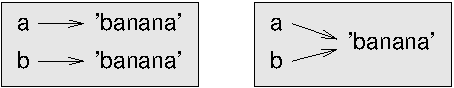
\includegraphics[scale=0.8]{figs/list1.pdf}}
\caption{แผนภาพสถานะ.}
\label{fig.list1}
\end{figure}

ในกรณีที่หนึ่ง \texttt{a} และ \texttt{b} อ้างถึงออบเจ๊คต์ที่ต่างกันสองออบเจ๊คต์ที่มีค่าเหมือนกัน.
ในกรณีที่สอง ทั้ง\texttt{a} และ \texttt{b} อ้างถึงออบเจ๊คต์เดียวกัน.
\index{is operator}
\index{operator!is}
\index{ตัวดำเนินการ!is}

เพื่อจะตรวจดูว่าตัวแปรสองตัวอ้างถึงออบเจ๊คต์เดียวกันหรือไม่
เราสามารถใช้ตัวดำเนินการ \texttt{is} ได้.

\begin{verbatim}
>>> a = 'banana'
>>> b = 'banana'
>>> a is b
True
\end{verbatim}
%
ในตัวอย่างนี้ ไพธอนแค่สร้างออบเจ๊คต์สายอักขระขึ้นมาแค่หนึ่งออบเจ๊คต์
และทั้งตัวแปร \texttt{a} และ \texttt{b} ก็อ้างถึงมัน.
แต่ถ้าเราสร้างลิสต์ออกมา เราจะได้สองออบเจ๊คต์:

\begin{verbatim}
>>> a = [1, 2, 3]
>>> b = [1, 2, 3]
>>> a is b
False
\end{verbatim}
%
ดังนั้นแผนภาพสถานะแสดงได้ดังรูป~\ref{fig.list2}.
\index{state diagram}
\index{diagram!state}
\index{แผนภาพสถานะ}
\index{แผนภาพ!สถานะ}

\begin{figure}
\centerline
{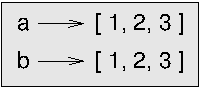
\includegraphics[scale=0.8]{figs/list2.pdf}}
\caption{แผนภาพสถานะ.}
\label{fig.list2}
\end{figure}

ในกรณีนี้ เราพูดได้ว่าลิสต์ทั้งสอง\textbf{เทียบเท่ากัน} (\textbf{equivalent})
เพราะว่า มันมีอิลิเมนต์ต่าง ๆ เหมือนกัน
แต่ไม่ใช่\textbf{เป็นอันเดียวกัน} (\textbf{identical})
เพราะว่ามันไม่ใช่ออบเจ๊คต์เดียวกัน.
ถ้าสองออบเจ๊คต์เป็นอันเดียวกันแล้ว มันจะเทียบเท่ากันด้วย
แต่ถ้ามันเทียบเท่ากัน มันไม่จำเป็นต้องเป็นอันเดียวกัน.
\index{equivalence}
\index{identity}
\index{การเทียบเท่ากัน}
\index{การเป็นอันเดียวกัน}

จนถึงตอนนี้ เราใช้คำว่า ``ออบเจ๊คต์'' และ ``ค่า'' สลับกันไปมาได้
แต่มันจะถูกต้องมากกว่าที่จะพูดว่าออบเจ๊คต์มีค่า.
%
ถ้าเราประเมินค่า \texttt{[1, 2, 3]}
เราจะได้ลิสต์ของออบเจ๊คต์ที่มีค่าเป็นลำดับของเลขจำนวนเต็มออกมา.  
ถ้าอีกลิสต์หนึ่งมีอิลิเมนต์เหมือน ๆ กัน เราพูดได้ว่ามันมีค่าเหมือนกัน
แต่มันไม่ใช่ออบเจ๊คต์เดียวกัน.
\index{object}
\index{value}
\index{ออบเจ๊คต์}
\index{ค่า}


\section{การทำสมนาม}
\index{aliasing}
\index{reference!aliasing}
\index{การอ้างอิง!การทำสมนาม}

ถ้าตัวแปร \texttt{a} อ้างอิงออบเจ๊คต์
และเรากำหนดให้ $\texttt{b = a}$
แล้วตัวแปรทั้งคู่จะอ้างอิงถึงออบเจ๊คต์เดียวกัน:

\begin{verbatim}
>>> a = [1, 2, 3]
>>> b = a
>>> b is a
True
\end{verbatim}
%
แผนภาพสถานะจะเป็นดังแสดงในรูป~\ref{fig.list3}.
\index{state diagram}
\index{diagram!state}
\index{แผนภาพสถานะ}
\index{แผนภาพ!สถานะ}

\begin{figure}
\centerline
{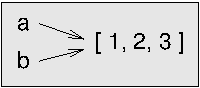
\includegraphics[scale=0.8]{figs/list3.pdf}}
\caption{แผนภาพสถานะ.}
\label{fig.list3}
\end{figure}

ความเกี่ยวข้องของตัวแปรกับออบเจ๊คต์จะเรียกว่า \textbf{การอ้างอิง} (\textbf{reference}).
ในตัวอย่างนี้ มีสองการอ้างอิงไปที่ออบเจ๊คต์เดียวกัน.
\index{reference}
\index{การอ้างอิง}

ออบเจ๊คต์ที่มีมากกว่าหนึ่งการอ้างอิง จะมีมากกว่าหนึ่งชื่อ
ดังนั้น เราจะเรียกว่า ออบเจ๊คต์ถูกทำ\textbf{สมนาม} (\textbf{aliased}).
\index{mutability}

ถ้าออบเจ๊คต์ที่ถูกทำสมนาม (อ้างถึงได้จากหลายชื่อ) สามารถเปลี่ยนแปลงค่าได้ (mutable)
การเปลี่ยนแปลงที่ทำกับชื่อหนึ่ง จะมีผลไปที่ชื่ออื่น ๆ ด้วย:

\begin{verbatim}
>>> b[0] = 42
>>> a
[42, 2, 3]
\end{verbatim}
%
แม้ว่าพฤติกรรมนี้จะมีประโยชน์
แต่มันก็มีแนวโน้มจะสร้างปัญหาอยู่มาก.
โดยทั่วไป มันจะปลอดภัยกว่าที่จะหลีกเลี่ยงการทำสมนามกับออบเจ๊คต์ที่เปลี่ยนแปลงค่าได้ (mutable objects).
\index{immutability}
\index{ความสามารถในการเปลี่ยนแปลงค่าได้}

สำหรับออบเจ๊คต์ที่เปลี่ยนแปลงค่าไม่ได้ เช่น สายอักขระ
การทำสมนามจะไม่ได้เป็นปัญหาอะไรมาก.
ในตัวอย่างนี้:

\begin{verbatim}
a = 'banana'
b = 'banana'
\end{verbatim}
%
มันแทบจะไม่ต่างเลยว่า \texttt{a} และ \texttt{b} อ้างถึงสายอักขระเดียวกันหรือไม่.

\section{อาร์กิวเมนต์ที่เป็นลิสต์}
\label{list.arguments}
\index{list!as argument}
\index{argument}
\index{argument!list}
\index{reference}
\index{parameter}
\index{ลิสต์!ใช้เป็นอาร์กิวเมนต์}
\index{อาร์กิวเมนต์}
\index{อาร์กิวเมนต์!ลิสต์}
\index{การอ้างอิง}
\index{พารามิเตอร์}

เมื่อเราส่งลิสต์เข้าไปให้กับฟังก์ชัน
ฟังก์ชันจะได้การอ้างอิงถึงลิสต์ (เป็นการอ้างอิงถึงลิสต์เดิมด้วยชื่อใหม่ ไม่ใช่ได้ลิสต์ใหม่).
ดังนั้นถ้าภายในฟังก์ชันมีการแก้ไขค่าของลิสต์
โปรแกรมที่เรียกฟังก์ชันจะเห็นการเปลี่ยนแปลงค่าของลิสต์นี้ด้วย.
ตัวอย่างเช่น \verb|delete_head| ลบอิลิเมนต์แรกออกจากลิสต์:

\begin{verbatim}
def delete_head(t):
    del t[0]
\end{verbatim}
%
และนี่คือตัวอย่างการเรียกใช้ฟังก์ชัน:
%
\begin{verbatim}
>>> letters = ['a', 'b', 'c']
>>> delete_head(letters)
>>> letters
['b', 'c']
\end{verbatim}
%
พารามิเตอร์ \texttt{t} (ในฟังก์ชัน) กับตัวแปร \texttt{letters} (ในโปรแกรมที่เรียกฟังก์ชัน เช่น \verb|__main__|) เป็นสมนามของออบเจ๊คต์เดียวกัน.
แผนภาพกองซ้อนแสดงในรูป~\ref{fig.stack5}.
\index{stack diagram}
\index{diagram!stack}
\index{แผนภาพกองซ้อน}

\begin{figure}
\centerline
{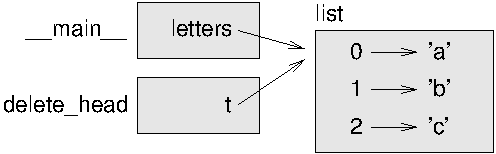
\includegraphics[scale=0.8]{figs/stack5.pdf}}
\caption{แผนภาพกองซ้อน.}
\label{fig.stack5}
\end{figure}

เนื่องจากลิสต์ถูกอ้างถึงจางทั้งสองตัวแปร ในภาพจึงวาดให้ลิสต์อยู่ระหว่างทั้งสองตัว.

มันสำคัญที่จะรู้ความแตกต่างระหว่าง
\textit{การดำเนินการ}ที่แก้ไขลิสต์
และ
\textit{การดำเนินการ}ที่สร้างลิสต์ใหม่.
ตัวอย่าง เมธอด \texttt{append} แก้ไขลิสต์
แต่ตัวดำเนินการ \texttt{+} สร้างลิสต์ใหม่.
\index{append method}
\index{method!append}
\index{list!concatenation}
\index{concatenation!list}
\index{เมธอด!append}
\index{ลิสต์!การต่อ}
\index{ลิสต์!การรวม}

ตัวอย่างการใช้ \texttt{append}:
%
\begin{verbatim}
>>> t1 = [1, 2]
>>> t2 = t1.append(3)
>>> t1
[1, 2, 3]
>>> t2
None
\end{verbatim}
%
ค่าที่ให้ออกมาจาก \texttt{append} คือ \texttt{None}.

ตัวอย่างการใช้ตัวดำเนินการ \texttt{+}:
%
\begin{verbatim}
>>> t3 = t1 + [4]
>>> t1
[1, 2, 3]
>>> t3
[1, 2, 3, 4]
\end{verbatim}
%
ผลลัพธ์จากตัวดำเนินการจะเป็นลิสต์ใหม่
และลิสต์เดิมไม่ได้เปลี่ยนอะไรไป.

ความต่างนี้สำคัญมาก ถ้าเราเขียนฟังก์ชันที่อาจมีการแก้ไขลิสต์.
ตัวอย่าง ฟังก์ชันข้างล่างนี้\emph{ไม่ได้}ลบหัวของลิสต์ออก:
%
\begin{verbatim}
def bad_delete_head(t):
    t = t[1:]              # WRONG!
\end{verbatim}
%
ตัวดำเนินการตัดลิสต์ (slice operator) สร้างลิสต์ใหม่ขึ้นมา
และการกำหนดค่าได้กำหนดให้ตัวแปร \texttt{t} อ้างถึงลิสต์ใหม่นี้.
แต่ทั้งหมดนี้ไม่ได้มีผลกับโปรแกรมที่เรียกฟังก์ชันนี้เลย.
\index{slice operator}
\index{operator!slice}
\index{ตัวดำเนินการ!การตัดช่วง}
\index{ลิสต์!การตัด}
%
\begin{verbatim}
>>> t4 = [1, 2, 3]
>>> bad_delete_head(t4)
>>> t4
[1, 2, 3]
\end{verbatim}
%
ในตอนเริ่มต้นฟังก์ชัน \verb|bad_delete_head| ตัวแปร \texttt{t} (ในฟังก์ชัน) และตัวแปร \texttt{t4} (ในโปรแกรมหลัก) อ้างถึงลิสต์เดียวกัน.
แต่ตอนท้าย ตัวแปร \texttt{\tt t} อ้างถึงลิสต์ใหม่
ในขณะที่ตัวแปร \texttt{t4} ยังอ้างถึงลิสต์เดิมอยู่ ลิสต์เดิมที่ไม่ได้ถูกแก้ไข.

วิธีที่ดีกว่า คือ เขียนฟังก์ชันที่สร้างและให้ค่าของลิสต์ใหม่ออกมา.
ตัวอย่างเช่น ฟังก์ชัน \texttt{tail} ให้ค่าของลิสต์ออกมาทั้งหมด ยกเว้นอิลิเมนต์แรกสุด::

\begin{verbatim}
def tail(t):
    return t[1:]
\end{verbatim}
%
ฟังก์ชันนี้ก็ไม่ได้เปลี่ยนลิสต์ดั่งเดิม.
วิธีเรียกใช้มันคือ:

\begin{verbatim}
>>> letters = ['a', 'b', 'c']
>>> rest = tail(letters)
>>> rest
['b', 'c']
\end{verbatim}



\section{การดีบัก}
\index{debugging}
\index{การดีบัก}

การใช้ลิสต์อย่างไม่ระวัง (รวมถึงออบเจ๊คต์ที่สามารถแก้ไขค่าได้ชนิดอื่น ๆ ด้วย)
อาจนำไปสู่ปัญหาที่ใช้เวลานานมากในการดีบัก.
ต่อไปนี้เป็นตัวอย่างของความผิดพลาดที่พบบ่อย และวิธีที่จะหลีกเลี่ยง:

\begin{enumerate}

\item เมธอดของลิสต์เกือบทั้งหมดแก้ค่าในอาร์กิวเมนต์ และมักส่งค่า \texttt{None} ออกมา (\texttt{return None}).
พฤติกรรมนี้จะต่างจากเมธอดของสายอักขระ ที่มักส่งสายอักขระใหม่ออกมา โดยไม่ไปยุ่งกับสายอักขระเดิม.

ถ้าเคยเขียนโปรแกรมแบบนี้:

\begin{verbatim}
word = word.strip()
\end{verbatim}

มันอาจจะมีแนวโน้มที่จะเขียนโปรแกรมกับลิสต์แบบนี้:

\begin{verbatim}
t = t.sort()           # WRONG!
\end{verbatim}
\index{sort method}
\index{method!sort}
\index{เมธอด!sort}

แต่เมธอด \texttt{sort} ส่งค่า \texttt{None} ออกมา
หลังจากนั้น ไม่ว่าเราจะทำอะไรกับตัวแปร \texttt{t} ก็ไม่น่าจะได้เรื่องอะไร.

ก่อนจะใช้เมธอดหรือตัวดำเนินการใด ๆ ของลิสต์
ให้อ่านเอกสารให้ถี่ถ้วน และทดสอบเมธอดหรือตัวดำเนินการเหล่านั้น ในการทำงานแบบโต้ตอบ (interactive mode) ก่อน.

\item เลือกรูปแบบการเขียนและยึดติดกับมัน.

ส่วนหนึ่งของปัญหาของการทำงานกับลิสต์ คือ มีวิธีที่จะทำงานหลายวิธีมาก.
ตัวอย่างเช่น การลบอิลิเมนต์จากลิสต์ เราสามารถใช้ \texttt{pop} หรือ \texttt{remove} หรือ \texttt{del} หรือแม้แต่จะใช้การกำหนดค่าและการตัดลิสต์ (slice assignment).

การเพิ่มอิลิเมนต์เอง เราก็สามารถใช้เมธอด \texttt{append} หรือตัวดำเนินการ \texttt{+}. 
สมมติว่า \texttt{t} เป็นลิสต์และ
\texttt{x} เป็นสมาชิกของลิสต์
วิธีเพิ่มอิลิเมนต์ข้างล่างนี้ถูกต้อง: 

\begin{verbatim}
t.append(x)
t = t + [x]
t += [x]
\end{verbatim}

แต่วิธีข้างล่างนี้ผิด:

\begin{verbatim}
t.append([x])          # WRONG!
t = t.append(x)        # WRONG!
t + [x]                # WRONG!
t = t + x              # WRONG!
\end{verbatim}

ลองตัวอย่างแต่ละอันในการทำงานแบบโต้ตอบ เพื่อให้แน่ใจว่าเข้าใจการทำงานของมันก่อน.
สังเกตว่า มีเฉพาะตัวอย่างสุดท้าย (\verb|t = t + x|) ที่ให้ \texttt{runtime error} ออกมา
อีกสามตัวอย่างข้างต้น แม้ว่าไม่ได้ให้ \texttt{runtime error} ออกมา แต่มันทำงานผิดจากที่เราต้องการ.

\item คัดลอก (copy) เพื่อเลี่ยงปัญหาจากการทำสมนาม
\index{aliasing!copying to avoid}
\index{copy!to avoid aliasing}
\index{การทำสมนาม!copy เพื่อเลี่ยงปัญหา}
\index{copy!เพื่อเลี่ยงปัญหาการทำสมนาม}

เช่น ถ้าหากเราต้องการใช้เมธอดอย่าง \texttt{sort} ที่แก้ไขข้อมูลของลิสต์
แต่ถ้าเราต้องการเก็บข้อมูลเดิมของลิสต์ไว้ด้วย
เราสามารถใช้การคัดลอกทำสำเนาไว้ได้.
%If you want to use a method like {\tt sort} that modifies
%the argument, but you need to keep the original list as
%well, you can make a copy.

\begin{verbatim}
>>> t = [3, 1, 2]
>>> t2 = t[:]
>>> t2.sort()
>>> t
[3, 1, 2]
>>> t2
[1, 2, 3]
\end{verbatim}

ตัวอย่างนี้ เราสามารถใช้ฟังก์ชันสำเร็จที่มีอยู่ในตัว \texttt{sorted} ก็ได้
ซึ่งฟังก์ชันนี้ให้ค่าลิสต์ใหม่ที่จัดเรียงแล้วออกมา โดยไม่ไปเปลี่ยนแปลงลิสต์เดิม.
\index{sorted!function}
\index{function!sorted}
\index{ฟังก์ชัน!sorted}

\begin{verbatim}
>>> t2 = sorted(t)
>>> t
[3, 1, 2]
>>> t2
[1, 2, 3]
\end{verbatim}

\end{enumerate}



\section{อภิธานศัพท์}

\begin{description}

\item[ลิสต์ (list):] ข้อมูลค่าต่าง ๆ ในลักษณะลำดับ.
\index{list}
\index{ลิสต์}

\item[อิลิเมนต์ (element):] ข้อมูลค่าแต่ละค่าในลิสต์ (หรือ รวมไปถึงแต่ละค่าของข้อมูลลักษณะลำดับแบบอื่น ๆ) บางครั้งอาจเรียก ค่ารายการ (item).
\index{element}
\index{อิลิเมนต์}

\item[ลิสต์ซ้อนใน (nested list):] ลิสต์ที่เป็นอิลิเมนต์ของอีกลิสต์.
\index{nested list}
\index{ลิสต์ซ้อนใน}

\item[ตัวสะสม (accumulator):] ตัวแปรที่ใช้ในลูป เพื่อเพิ่มค่า หรือเพื่อเก็บสะสมผลลัพธ์.
\index{accumulator}
\index{ตัวสะสม}

\item[การกำหนดเสริมค่า (augmented assignment):] ข้อความคำสั่งที่แก้ไขค่าของตัวแปร โดยใช้ตัวดำเนินการ เช่น \verb|+=|.
\index{assignment!augmented}
\index{augmented assignment}
\index{traversal}
\index{การกำหนดค่า!เสริมค่า}
\index{การกำหนดเสริมค่า}
\index{การท่องสำรวจ}


\item[การยุบ (reduce):] รูปแบบการประมวลผลที่สำรวจค่าต่าง ๆ ในลำดับ และรวมสรุปค่าอิลิเมนต์ต่าง ๆ มาเป็นค่า ๆ เดียว.
\index{reduce pattern}
\index{pattern!reduce}
\index{การยุบ}
\index{รูปแบบ!การยุบ}


\item[การแปลง (map):] รูปแบบการประมวลผลที่สำรวจค่าต่าง ๆ ในลำดับ และทำการดำเนินการกับอิลิเมนต์แต่ละตัว.
\index{map pattern}
\index{pattern!map}
\index{การแปลง}
\index{รูปแบบ!การแปลง}

\item[การกรอง (filter):] รูปแบบการประมวลผลที่สำรวจค่าต่าง ๆ ในลำดับ และเลือกเฉพาะอิลิเมนต์ที่ผ่านเงื่อนไขออกมา.
\index{filter pattern}
\index{pattern!filter}
\index{การกรอง}
\index{รูปแบบ!การกรอง}


\item[ออบเจ๊คต์ (object):] สิ่งที่ตัวแปรอ้างถึงได้.  
ออบเจ๊คต์มีชนิดและค่า.
\index{object}
\index{ออบเจ๊คต์}


\item[เทียบเท่ากัน (equivalent):] มีค่าเหมือนกัน (แต่ไม่จำเป็นต้องเป็นออบเจ๊คต์อันเดียวกัน).
\index{equivalence}
\index{equivalent}
\index{การเทียบเท่ากัน}

\item[เป็นอันเดียวกัน (identical):] เป็นออบเจ๊คต์เดียวกัน.
% (which implies equivalence).
\index{identical}
\index{เป็นอันเดียวกัน}

\item[การอ้างอิง (reference):] ความเกี่ยวเนื่องเชื่อมโยงกันของตัวแปรและค่าของมัน.
\index{reference}
\index{การอ้างอิง}

\item[การทำสมนาม (aliasing):] สถานการณ์ที่ตัวแปรมากกว่าสองตัวขึ้นไปอ้างถึงออบเจ๊คต์เดียวกัน.
\index{aliasing}
\index{การทำสมนาม}

\item[ตัวแบ่งคำ (delimiter):] ตัวอักษร หรือสายอักขระ ที่ใช้เพื่อระบุว่า สายอักขระทั้งหมดควรจะถูกแบ่งที่ใด.
\index{delimiter}
\index{ตัวแบ่งคำ}

\end{description}


\section{แบบฝึกหัด}

ผู้อ่านสามารถดาวน์โหลดเฉลยของแบบฝึกหัดเหล่านี้ได้จาก
\url{http://thinkpython2.com/code/list_exercises.py}.
\\

\begin{exercise}

จงเขียนฟังก์ชัน ชื่อ \verb|nested_sum| ที่รับลิสต์ของลิสต์ของเลขจำนวนเต็ม
และบวกค่าอิลิเมนต์จากทุกลิสต์ซ้อนในทั้งหมด.
ตัวอย่าง:

\begin{verbatim}
>>> t = [[1, 2], [3], [4, 5, 6]]
>>> nested_sum(t)
21
\end{verbatim}

\end{exercise}
\vspace{0.5cm}


\begin{exercise}
\label{cumulative}
\index{cumulative sum}
\index{การบวกสะสม}

จงเขียนฟังก์ชัน ชื่อ \texttt{cumsum} ที่รับลิสต์ของตัวเลข
และให้ค่าผลบวกสะสมออกมา 
นั่นคือ ลิสต์ใหม่ที่เป็นผลลัพธ์มีอิลิเมนต์ที่ $i$ เป็นผลรวมของอิลิเมนต์ $i+1$ ตัวแรกของลิสต์ต้นฉบับ.
ตัวอย่าง:


\begin{verbatim}
>>> t = [1, 2, 3]
>>> cumsum(t)
[1, 3, 6]
\end{verbatim}

\end{exercise}
\vspace{0.5cm}


\begin{exercise}
จงเขียนฟังก์ชัน ชื่อ \texttt{middle} ที่รับลิสต์
และให้ค่าลิสต์ใหม่ออกมา
โดยที่ลิสต์ใหม่นั้นมีอิลิเมนต์อื่น ๆ เหมือนกับลิสต์ที่ใส่เข้าไป แต่ไม่มีอิลิเมนต์แรก ไม่มีอิลิเมนต์สุดท้าย.
ตัวอย่าง:

\begin{verbatim}
>>> t = [1, 2, 3, 4]
>>> middle(t)
[2, 3]
\end{verbatim}

\end{exercise}
\vspace{0.5cm}


\begin{exercise}

จงเขียนฟังก์ชัน ชื่อ \texttt{chop} ที่รับลิสต์ 
แล้วไปแก้ไขค่าของมัน โดยลบอิลิเมนต์แรกสุด และลบอิลิเมนต์ท้ายสุดออก.
ฟังก์ชันนี้ให้ค่า \texttt{None} ออกมา.
ตัวอย่าง:

\begin{verbatim}
>>> t = [1, 2, 3, 4]
>>> chop(t)
>>> t
[2, 3]
\end{verbatim}

\end{exercise}
\vspace{0.5cm}


\begin{exercise}
จงเขียนฟังก์ชัน ชื่อ \verb|is_sorted|
ที่รับลิสต์ 
และส่งค่า \texttt{True} ออกมา ถ้าลิสต์ถูกเรียงลำดับจากน้อยไปมาก
และส่งค่า \texttt{False} ออกมา ถ้าไม่ใช่.  
ตัวอย่าง:

\begin{verbatim}
>>> is_sorted([1, 2, 2])
True
>>> is_sorted(['b', 'a'])
False
\end{verbatim}

\end{exercise}
\vspace{0.5cm}


\begin{exercise}
\label{anagram}
\index{anagram}

คำสองคำจะเรียกว่าเป็น อนาแกรม (anagrams) 
ถ้าเราสามารถเรียงตัวอักษรในคำหนึ่งให้สะกดเป็นอีกคำได้
จงเขียนฟังก์ชัน ชื่อ \verb|is_anagram|
ที่รับสายอักขระสองสาย และให้ค่า \texttt{True} ออกมา ถ้าสายอักขระทั้งสองเป็นอนาแกรม.
\end{exercise}
\vspace{0.5cm}


\begin{exercise}
\label{duplicate}
\index{duplicate}
\index{uniqueness}

จงเขียนฟังก์ชัน ชื่อ \verb|has_duplicates| 
ที่รับลิสต์ และให้ค่า \texttt{True} ออกมา
ถ้ามีอิลิเมนต์ในลิสต์ที่ปรากฏมากกว่าหนึ่งครั้ง.
ฟังก์ชันนี้ไม่เปลี่ยนแปลงค่าลิสต์ต้นฉบับ.

\end{exercise}
\vspace{0.5cm}


\begin{exercise}
แบบฝึกหัดนี้เกี่ยวกับ ปฏิทรรศน์วันเกิด (Birthday Paradox ซึ่งศึกษาเพิ่มเติมได้จาก \url{http://en.wikipedia.org/wiki/Birthday_paradox}).
\index{birthday paradox}

ถ้ามีนักเรียนในห้อง 23 คน มีโอกาสที่จะมีนักเรียนสองคนที่วันเกิดตรงกันเป็นเท่าไร
จงประมาณความน่าจะเป็น โดยสร้างตัวอย่างสุ่มของวันเกิด 23 วัน และตรวจสอบว่ามีวันตรงกันหรือไม่.
คำใบ้: เราสามารถสร้างตัวอย่างวันเกิดสุ่มได้ด้วยฟังก์ชัน \texttt{randint} ในโมดูล \texttt{random}.
\index{random module}
\index{module!random}
\index{randint function}
\index{function!randint}
\index{โมดูล!random}
\index{ฟัังชั่น!randint}

เฉลยดาวน์โหลดได้จาก \url{http://thinkpython2.com/code/birthday.py}.

\end{exercise}
\vspace{0.5cm}


\begin{exercise}
\index{append method}
\index{method append}
\index{list!concatenation}
\index{concatenation!list}
\index{ลิสต์!การต่อ}

จงเขียนฟังก์ชันที่อ่านไฟล์ \texttt{words.txt} (ดาวน์โหลดไฟล์ได้จาก \url{http://greenteapress.com/thinkpython2/code/words.txt}) และสร้างลิสต์ที่แต่ละอิลิเมนต์เป็นแต่ละคำในไฟล์.
เขียนฟังก์ชันเป็นสองแบบ
แบบแรกใช้เมธอด \texttt{append}
และอีกแบบใช้ \texttt{t = t + [x]}.
แบบไหนใช้เวลารันนานกว่า? ทำไม?

เฉลย: \url{http://thinkpython2.com/code/wordlist.py}.
\index{time module}
\index{module!time}
\index{โมดูล!time}

\end{exercise}
\vspace{0.5cm}


\begin{exercise}
\label{wordlist1}
\label{bisection}
\index{membership!bisection search}
\index{bisection search}
\index{search, bisection}
\index{membership!binary search}
\index{binary search}
\index{search, binary}
\index{วิธีค้นหาแบ่งสองส่วน}

เพื่อตรวจสอบว่าคำอยู่ในลิสต์ของคำหรือไม่
เราควรจะใช้ตัวดำเนินการ \texttt{in}
แต่มันจะทำงานช้า เพราะว่ามันตรวจโดยการค้นหาทีละอิลิเมนต์ตามลำดับ.

ถ้าเรารู้ว่าคำในลิสต์เรียงตามลำดับตัวอักษระอยู่แล้ว
เราสามารถทำให้การค้นหาเร็วขึ้นได้
ด้วยวิธีค้นหาแบ่งสองส่วน (bisection search หรืออีกชื่อ binary search).
วิธีค้นหาแบ่งสองส่วน คล้ายกับวิธีที่เราทำ เวลาที่เราหาคำในพจนานุกรม.
เราเริ่มที่ตรงกลาง และดูว่าคำที่เราหามาก่อนหรือหลังคำที่ตรงกลางลิสต์.
ถ้าคำที่หามาก่อน ก็ให้ไปหาในครึ่งหน้าด้วยแนวทางนี้อีก
ถ้าคำที่หามาหลัง ก็ให้ไปหาในครึ่งหลัง.
ไม่ว่าอย่างไร เราก็ลด\textit{ปริภูมิค้นหา}(\textit{search space})ลงไปครึ่งหนึ่ง.
ถ้าในลิสต์ของคำมีคำอยู่ 113,809 คำ มันจะใช้แค่ประมาณ 17 ขั้น เพื่อหาคำให้เจอ หรือเพื่อบอกว่าคำนั้นไม่อยู่ในลิสต์.

จงเขียนฟังก์ชัน \verb|in_bisect| ที่รับลิสต์ที่เรียงลำดับไว้แล้ว
กับรับค่าที่ต้องการค้นหา
แล้วส่งดัชนีของค่าที่หาออกมาถ้าลิสต์มีค่านั้นอยู่
หรือส่งค่า \texttt{None} ออกมา ถ้าลิสต์ไม่มีค่าที่หา.
\index{bisect module}
\index{module!bisect}
\index{โมดูล!bisect}

หรือ อ่านเอกสารของโมดูล \texttt{bisect} และเรียกใช้!  
เฉลย: \url{http://thinkpython2.com/code/inlist.py}.

\end{exercise}
\vspace{0.5cm}


\begin{exercise}
\index{reverse word pair}

คำสองคำเป็น ``คู่กลับ'' (reverse pair) ถ้าคำหนึ่งเป็นคำเรียงกลับของอีกคำหนึ่ง.
จงเขียนโปรแกรมที่หาคู่กลับทั้งหมดในลิสต์ของคำ.
เฉลย: \url{http://thinkpython2.com/code/reverse_pair.py}.

\end{exercise}
\vspace{0.5cm}


\begin{exercise}
\index{interlocking words}

คำสองคำจะเรียกว่า ``เกี่ยวติดกัน'' (interlock) ถ้านำอักษรจากแต่ละคำมาเรียงสลับกันแล้วได้คำใหม่.
ตัวอย่างเช่น ``shoe'' และ ``cold''
เกี่ยวติดกันแล้วได้คำใหม่คือ ``schooled''.
เฉลย: \url{http://thinkpython2.com/code/interlock.py}.
ให้เกียรติ: แบบฝึกหัดนี้ได้รับแรงบันดาลใจจากตัวอย่างใน \url{http://puzzlers.org}.

\begin{enumerate}

\item กำหนดให้ลิสต์ของคำ (ใช้ลิสต์ของคำจากไฟล์ตัวอย่าง \texttt{words.txt} ได้) จงเขียนโปรแกรมที่หาทุกคู่ของคำในลิสต์ ที่เกี่ยวติดกันเป็นคำใหม่ ที่ก็อยู่ในลิสต์.
คำใบ้: ไม่ต้องนับทุกคู่ (เราอาจหาคำที่เกี่ยวติดกันจากคำสองคู่ว่าอยู่ในลิสต์หรือไม่ 
หรืออาจดูว่าคำในลิสต์ว่าแยกออกมาเป็นคำสองคำอะไร)

\item คุณหาคำต่าง ๆ ที่\textit{เกี่ยวติดกันสามทาง}ได้หรือเปล่า?
คำที่\textit{เกี่ยวติดกันสามทาง} (\textit{three-way interlocked}) ได้มาจากสามคำโดย
อักษรในคำได้จากคำต้นฉบับทั้งสามเรียงสลับกัน เช่น powered ได้จากการเกี่ยวติดกันสามทางของ ped และ or และ we เป็นต้น.

\end{enumerate}
\end{exercise}
\vspace{0.5cm}


\chapter{ดิกชันนารี}

บทนี้นำเสนอ\textit{ชนิดข้อมูลในตัว} (\textit{built-in type}) อีกชนิด ที่เรียกว่า ดิกชันนารี (dictionary).
ดิกชันนารี เป็นลักษณะเฉพาะของไพธอนที่จัดว่าดีที่สุดอันหนึ่ง
มันเป็นเสมือนส่วนประกอบพื้นฐานของอัลกอริทึมที่มีประสิทธิภาพที่แจ๋ว ๆ ต่าง ๆ.

\section{ดิกชันนารีเป็นการแปลง}

\index{dictionary}
\index{dictionary}
\index{type!dict}
\index{key}
\index{key-value pair}
\index{index}
\index{ดิกชันนารี}
\index{ชนิดข้อมูล!ดิกชันนารี}
\index{ชนิดข้อมูล!dict}
\index{ดัชนี}

\textbf{ดิกชันนารี}คล้ายกับลิสต์ แต่ใช้งานได้กว้างขวางกว่า.
%\footnote{%
%ในมุมที่ ดิกชันนารี ยอมให้ผู้ใช้กำหนดดัชนีเองได้}.
สำหรับลิสต์ ดัชนีต้องเป็นเลขจำนวนเต็มเท่านั้น
แต่ดิกชันนารีสามารถกำหนดใช้ดัชนีเป็นข้อมูลใดก็ได้ (เกือบทุกชนิด).

ดิกชันนารีประกอบไปด้วยกลุ่มหมู่ของดัชนีต่าง ๆ เรียกว่า \textbf{กุญแจ} (\textbf{keys}) และกลุ่มหมู่ของค่าต่าง ๆ ที่เชื่อมโยงกับดัชนี.
แต่ละกุญแจจะเชื่อมไปหาค่า (value).
การเชื่อมโยงระหว่างกุญแจกับค่าจะเรียกว่า \textbf{คู่กุญแจกับค่า} (\textbf{key-value pair}) หรือบางครั้งอาจเรียก \textbf{รายการ} (\textbf{item}).  
\index{item}
\index{รายการ}

หากพูดในเชิงคณิตศาสตร์ ดิกชันนารีก็คือ\textbf{การแปลง} (\textbf{mapping}) จาก กุญแจ (keys) ไปเป็น ค่า (values)
ซึ่งเราสามารถพูดได้ว่า แต่ละดัชนีกุญแจ ``แปลงไปเป็น'' ค่า.
ดังตัวอย่างนี้ เราจะสร้างดิกชันนารีที่แปลงจากคำในภาษาอังกฤษไปเป็นคำในภาษาสเปน
ดังนั้น ทั้งกุญแจและค่า จะเป็นชนิดข้อมูลสายอักขระ.

ฟังก์ชัน \texttt{dict} สร้างดิกชันนารีใหม่ขึ้นมา โดยยังไม่มีรายการใด ๆ อยู่ภายใน.
เนื่องจาก \texttt{dict} เป็นชื่อของฟังก์ชันสำเร็จ
เราจึงต้องไม่ใช้มันไปตั้งเป็นชื่อตัวแปร.
\index{dict function}
\index{function!dict}
\index{ฟังก์ชัน!dict}

\begin{verbatim}
>>> eng2sp = dict()
>>> eng2sp
{}
\end{verbatim}

วงเล็บหยัก ๆ \verb|{}| แทนดิกชันนารีที่ว่างอยู่.
เพื่อจะเพิ่มรายการเข้าไปในดิกชันนารี เราสามารถใช้วงเล็บสี่เหลี่ยมดังนี้:
\index{squiggly bracket}
\index{bracket!squiggly}\index{วงเล็บ!หยัก}

\begin{verbatim}
>>> eng2sp['one'] = 'uno'
\end{verbatim}
%
คำสั่งบรรทัดนี้สร้างรายการขึ้นมา
โดยแปลงจากกุญแจ \verb|'one'| ไปเป็นค่า \verb|'uno'|.
ถ้าเราสั่งพิมพ์ค่าดิกชันนารีออกมาดู
เราจะเห็น รายการคู่กุญแจค่า ที่มีเครื่องจุดคู่ (ทวิภาค หรือ colon) คั่นระหว่างกุญแจกับค่า:

\begin{verbatim}
>>> eng2sp
{'one': 'uno'}
\end{verbatim}
%
รูปแบบเอาต์พุตนี้ ก็สามารถใช้เป็นรูปแบบอินพุตได้
เช่น เราสามารถสร้างดิกชันนารีใหม่ ที่มีสามรายการได้ดังนี้:

\begin{verbatim}
>>> eng2sp = {'one': 'uno', 'two': 'dos', 'three': 'tres'}
\end{verbatim}
%
แต่ถ้าเราสั่งพิมพ์ \texttt{eng2sp} ออกมาดู เราอาจจะแปลกใจที่เห็น:

\begin{verbatim}
>>> eng2sp
{'one': 'uno', 'three': 'tres', 'two': 'dos'}
\end{verbatim}
%
ลำดับของรายการคู่กุญแจค่าอาจจะไม่เหมือนเดิม.
หรือแม้แต่เวลาที่คุณไปทดลองตัวอย่างนี้ในเครื่องของคุณ คุณก็อาจจะได้ผลลัพธ์ต่างออกไปก็ได้.
โดยทั่วไปแล้ว ลำดับของรายการในดิกชันนารี อาจเปลี่ยนแปลงไป.

แต่ลำดับของรายการในดิกชันนารีไม่ใช่ปัญหา 
เพราะว่ารายการต่าง ๆ ในดิกชั่นารีจะไม่ถูกอ้างจากดัชนีลำดับ.
สำหรับดิกชันนารี เราจะใช้ดัชนีกุญแจเพื่อหาค่าที่เป็นผูกกับมัน:

\begin{verbatim}
>>> eng2sp['two']
'dos'
\end{verbatim}
%
กุญแจ \verb|'two'| จะแปลงไปเป็นค่า \verb|'dos'| เสมอ
ดังนั้น ลำดับของรายการจึงไม่สำคัญ.

ถ้าหากกุญแจไม่มีอยู่ในดิกชันนารี เราจะได้รับแจ้งข้อผิดพลาดมาแทน.
\index{exception!KeyError}
\index{KeyError}

\begin{verbatim}
>>> eng2sp['four']
KeyError: 'four'
\end{verbatim}
%
ฟังก์ชัน \texttt{len} ก็ได้งานได้กับดิกชันนารี
มันจะให้ค่าจำนวนของรายการคู่กุญแจค่าออกมา:
\index{len function}
\index{function!len}
\index{ฟังก์ชัน!len}

\begin{verbatim}
>>> len(eng2sp)
3
\end{verbatim}
%
ตัวดำเนินการ \texttt{in} ก็ทำงานได้กับดิกชันนารี
มันจะบอกเราว่า สิ่งที่เราสงสัยมีปรากฏเป็น \emph{กุญแจ} (\emph{key}) ในดิกชันนารีหรือไม่ (ปรากฏเป็นค่าไม่นับ).
\index{membership!dictionary}
\index{in operator}
\index{operator!in}

\begin{verbatim}
>>> 'one' in eng2sp
True
>>> 'uno' in eng2sp
False
\end{verbatim}
%
เพื่อจะดูว่ามีอะไรเป็นค่าของกุญแจในดิกชันนารีบ้าง
เราสามารถใช้เมธอด \texttt{values} ที่ให้ค่ากุญแจต่าง ๆ ในดิกชันนารีออกมา
จากนั้น เราสามารถใช้ตัวดำเนินการ \texttt{in} ได้:
\index{values method}
\index{method!values}
\index{เมธอด!values}

\begin{verbatim}
>>> vals = eng2sp.values()
>>> 'uno' in vals
True
\end{verbatim}
%
ตัวดำเนินการ \texttt{in} ใช้อัลกอริทึมสำหรับดิกชันนารี ต่างกับอัลกอริทึมที่ใช้สำหรับลิสต์.
สำหรับลิสต์ มันจะค้นหาอิลิเมนต์ของลิสต์ตามลำดับ เช่นในหัวข้อ~\ref{find}.
ถ้าลิสต์ยาวขึ้น เวลาในการค้นหาก็จะนานขึ้น เวลาค้นหากับความยาวลิสต์เป็นสัดส่วนกันโดยตรง.

สำหรับดิกชันนารี ไพธอนใช้อัลกิริธึมที่เรียกว่า \textbf{ตารางแฮช} (\textbf{hashtable}) ซึ่งมีคุณสมบัติที่ยอดเยี่ยม.
นั่นคือ 
ตัวดำเนินการ \texttt{in} ใช้เวลาพอ ๆ กันในการค้นหา ไม่ว่าดิกชันนารีจะมีรายการอยู่มากเท่าไร.
รายละเอียดของ\textbf{ตารางแฮช}อธิบายอยู่ในหัวข้อ~\ref{hashtable}
แต่คำอธิบายอาจจะเข้าใจได้ยาก หากไม่ได้ศึกษาบทต่อ ๆ ไปก่อน.


\section{ดิกชันนารีเป็นกลุ่มหมู่ของตัวนับ}
\label{histogram}
\index{counter}

สมมติว่าเราได้สายอักขระมา และเราต้องการนับจำนวนว่าตัวอักษรแต่ละตัวมีปรากฎอยู่ในสายอักขระนั้นอีกครั้ง.
มีหลายวิธีที่เราทำได้ เช่น:

\begin{enumerate}

\item วิธีหนึ่ง เราอาจจะสร้างตัวแปรขึ้นมา 26 ตัวแปร แต่ละตัวแปรสำหรับแต่ละตัวอักษร.
แล้วเราก็จะเข้าไปไล่ดูภายในสายอักขระ
และนับจำนวนของแต่ละอักขระ 
ใช้ตัวแปรแต่ละตัวเก็บจำนวนนับของแต่ละตัวอักษร
โดยอาจจะใช้\textit{เงื่อนไขลูกโซ่} (คำสั่งพวก \texttt{if-elif-else}) ช่วย.

\item วิธีหนึ่ง เราสามารถสร้างลิสต์ที่มี 26 อิลิเมนต์ขึ้นมา.
แล้วเราก็แปลงตัวอักษรแต่ละตัวเป็นตัวเลข (อาจจะใช้ฟังก์ชันสำเร็จ \texttt{ord}) และใช้ตัวเลขที่ได้เป็นดัชนีของลิสต์ 
และเพิ่มจำนวนนับในลิสต์.

\item อีกวิธีหนึ่ง เราสามารถสร้างดิกชันนารี
ที่ใช้ตัวอักษรเป็นกุญแจ
และใช้ค่าของกุญแจเป็นจำนวนนับ.
เวลาที่เจอตัวอักษรเป็นครั้งแรก เราจะเพิ่มรายการเข้าไปในดิกต์.
หลังจากนั้น เราจะเพิ่มค่าจำนวนนับของอักษรตัวนั้น.

\end{enumerate}

แต่ละวิธีจะทำงานเดียวกัน
แต่ว่า ทำด้วยวิธีที่ต่างกัน.
\index{implementation}
\index{วิธีการสร้างโปรแกรม}

\textbf{วิธีการสร้างโปรแกรม} (\textbf{implementation}) 
เป็นวิธีที่จะทำงาน วิธีที่จะทำการคำนวณ วิธีที่จะเขียนโปรแกรม.
บางวิธีจะดีกว่าวิธีอื่น.
ตัวอย่าง เช่น 
ข้อดีของวิธีที่ใช้ดิกชันนารีคือ
เราไม่จำเป็นต้องรู้ก่อนว่า ตัวอักษรมีอยู่ในสายอักขระหรือไม่
เราแค่สร้างที่เก็บตัวนับให้มัน ถ้ามันมีปรากฏอยู่.
หน้าตาของโปรแกรมอาจจะเป็นดังนี้:

\begin{verbatim}
def histogram(s):
    d = dict()
    for c in s:
        if c not in d:
            d[c] = 1
        else:
            d[c] += 1
    return d
\end{verbatim}
%
ชื่อของฟังก์ชันข้างต้นคือ \texttt{histogram}
ซึ่งเป็นคำศัพท์ทางสถิติที่ใช้สำหรับกลุ่มหมู่ของตัวนับ (หรือ ความถี่).
\index{histogram}
\index{frequency}
\index{traversal}

บรรทัดแรกของฟังก์ชันสร้างดิกชันนารีว่าง ๆ ขึ้นมา.
คำสั่งลูป \texttt{for} ไล่สำรวจอักษรต่าง ๆ ในสายอักขระ.
แต่ละรอบในลูป ถ้าตัวอักษรของตัวแปร \texttt{c} ไม่อยู่ในดิกชันนารี
เราจะสร้างรายการใหม่ด้วยกุญแจ \texttt{c} และให้ค่าเริ่มต้นเป็น 1 (เนื่องจากเราเจอตัวอักษรแล้วหนึ่งครั้ง).
ถ้าตัวอักษรของตัวแปร \texttt{c} มีอยู่แล้วในดิกชันนารี เราก็เพิ่มค่า \texttt{d[c]}.
\index{histogram}

มันทำงานดังนี้:

\begin{verbatim}
>>> h = histogram('brontosaurus')
>>> h
{'a': 1, 'b': 1, 'o': 2, 'n': 1, 's': 2, 'r': 2, 'u': 2, 't': 1}
\end{verbatim}
%
ฮิสโตแกรมที่ได้บอกวว่า อักษร \verb|a| และอักษร \verb|b| มีปรากฎหนึ่งครั้ง 
อักษร \verb|o| มีปรากฎสองครั้ง เป็นต้น.

\index{get method}
\index{method!get}
\index{เมธอด!get}
ดิกชันนารีมีเมธอด \texttt{get} ที่รับกุญแจ และค่าโดยปริยาย (ค่าดีฟอลท์) ของมัน.
ถ้ากุญแจนั้นมีอยู่ในดิกชันนารีอยู่แล้ว
\texttt{get} จะให้ค่าของกุญแจนั้นออกมา
ไม่อย่างนั้นก็จะให้ค่าโดยปริยายออกมา.
ตัวอย่าง:

\begin{verbatim}
>>> h = histogram('a')
>>> h
{'a': 1}
>>> h.get('a', 0)
1
>>> h.get('b', 0)
0
\end{verbatim}
%
เพื่อเป็นการฝึกใช้ 
ให้ลองใช้ \texttt{get} เพื่อเขียน \texttt{histogram} ให้กระชับยิ่งขึ้น.
เราน่าจะสามารถเอาคำสั่ง \texttt{if} ออกไปได้.


\section{ลูปและดิกชันนารี}
\index{dictionary!looping with}
\index{looping!with dictionaries}
\index{traversal}
\index{ดิกชันนารี!ลูป}
\index{ลูป!ดิกชันนารี}

ถ้าเราใช้ดิกชันนารีในคำสั่ง \texttt{for}
มันจะท่องสำรวจกุญแจของดิกชันนารี.
ตัวอย่าง
\verb"print_hist"
พิมพ์กุญแจ และค่าของกุญแจ แต่ละรายการออกมา:

\begin{verbatim}
def print_hist(h):
    for c in h:
        print(c, h[c])
\end{verbatim}
%
ผลลัพธ์ที่ได้จะเป็นดังนี้:

\begin{verbatim}
>>> h = histogram('parrot')
>>> print_hist(h)
a 1
p 1
r 2
t 1
o 1
\end{verbatim}
%
ย้ำอีกครั้งว่า กุญแจจะไม่ได้เรียงตามลำดับใด ๆ
ถ้าหากต้องการทำลูปสำรวจกุญแจตามลำดับ เราสามารถใช้ฟังก์ชันสำเร็จ \texttt{sorted}:
\index{sorted!function}
\index{function!sorted}
\index{ฟังก์ชัน!sorted}

\begin{verbatim}
>>> for key in sorted(h):
...     print(key, h[key])
a 1
o 1
p 1
r 2
t 1
\end{verbatim}

%TODO: get this on Atlas


\section{การเทียบค้นย้อนกลับ}
\label{raise}
\index{dictionary!lookup}
\index{dictionary!reverse lookup}
\index{lookup, dictionary}
\index{reverse lookup, dictionary}
\index{ดิกชันนารี!เทียบค้น}
\index{ดิกชันนารี!เทียบค้นย้อนกลับ}

ถ้าให้ดิกชันนารี \texttt{d} และกุญแจ \texttt{k}
เราสามารถหาค่าของกุญแจ \texttt{v = d[k]} ได้ง่าย ๆ.
การดำเนินการแบบนี้เรียกว่า \textbf{การเทียบค้น} (\textbf{lookup}).

แต่หากเรามี \texttt{v} และต้องการหาค่า \texttt{k} หละ?
เราเจอปัญหาสองอย่างคือ: หนึ่ง มันอาจจะมีกุญแจมากกว่าหนึ่งกุญแจที่เชื่อมไปหาค่า \texttt{v} เหมือนกัน.
อันนี้ก็ขึ้นกับงาน เราอาจจจะเลือกสักกุญแจหนึ่ง 
หรือ เราอาจจะสร้างลิสต์ของกุญแจทั้งหมดของค่านั้นขึ้นมา.
สอง ไม่มีคำสั่งง่าย ๆ ที่จะทำ\textbf{การเทียบค้นย้อนกลับ}ให้
เราต้องค้นหาเอง.

ข้างล่างนี้ คือ ฟังก์ชันที่รับค่าของกุญแจ
และส่งกุญแจแรกที่เจอออกมา:
%Here is a function that takes a value and returns the first
%key that maps to that value:

\begin{verbatim}
def reverse_lookup(d, v):
    for k in d:
        if d[k] == v:
            return k
    raise LookupError()
\end{verbatim}
%
ฟังก์ชันนี้เป็นอีกตัวอย่างหนึ่งของการค้นหารูปแบบ
เพียงแต่ว่า มีการใช้คำสั่งใหม่ คำสั่ง \texttt{raise}.
\textbf{คำสั่ง raise} (\textbf{raise statement}) จะทำให้เกิดเอ็กเซ็ปชั่น (exception) ขึ้น
ในกรณีนี้ มันจะไปเรียก \texttt{LookupError} ซึ่งเป็นเอ็กเซ็ปชั่นสำเร็จรูป (built-in exception) เพื่อแจ้งว่าการดำเนินการเทียบค้นล้มเหลว.
\index{search}
\index{pattern!search} \index{raise statement} \index{statement!raise}
\index{exception!LookupError} \index{LookupError}
\index{การค้นหา}
\index{รูปแบบ!การค้นหา}

ถ้าเราค้นหาไปจนสุดจบลูป นั่นหมายความว่า \texttt{v} ไม่ได้ปรากฏเป็นค่าในดิกชันนารี
ดังนั้นเราจึงส่งเอ็กเซ็ปชั่นออกไป.


ตัวอย่างนี้แสดง การเทียบค้นย้อนกลับที่สำเร็จ:

\begin{verbatim}
>>> h = histogram('parrot')
>>> key = reverse_lookup(h, 2)
>>> key
'r'
\end{verbatim}
%
และนี่คือตัวอย่างอันที่ไม่สำเร็จ:

\begin{verbatim}
>>> key = reverse_lookup(h, 3)
Traceback (most recent call last):
  File "<stdin>", line 1, in <module>
  File "<stdin>", line 5, in reverse_lookup
LookupError
\end{verbatim}
%
ผลลัพธ์จากที่เราส่งเอ็กเซ็ปชั่นออกมา จะเหมือนกับตอนที่ไพธอนส่งออกมา:
มันจะพิมพ์ข้อความสืบย้อน (trackback message) และข้อความแสดงข้อผิดพลาดออกมา (error message).
\index{traceback}
\index{optional argument}
\index{argument!optional}

คำสั่ง \texttt{raise} สามารถรับข้อความแสดงข้อผิดพลาด เป็นอาร์กิวเมนต์เสริมได้.
ตัวอย่างเช่น:
%แปลจาก The raise statement can take a detailed error message as an optional argument. 

\begin{verbatim}
>>> raise LookupError('value does not appear in the dictionary')
Traceback (most recent call last):
  File "<stdin>", line 1, in ?
LookupError: value does not appear in the dictionary
\end{verbatim}
%
การเทียบค้นย้อนกลับจะช้ากว่าการเทียบค้นธรรมดามาก
ถ้าเราต้องทำบ่อย ๆ หรือถ้าดิกชันนารีมีขนาดใหญ่
ประสิทธิภาพของโปรแกรมจะแย่มาก.


\section{ดิกชันนารีและลิสต์}
\label{invert}

ลิสต์สามารถเป็นค่าในดิกชันนารีได้.
ตัวอย่างเช่น
ถ้าเราได้ดิกชันนารี ที่แปลงจากตัวอักษรไปเป็นความถี่
เราอาจจะต้องการทำผกผันมัน นั่นคือ สร้างดิกชันนารี
ที่แปลงจากความถี่ไปเป็นตัวอักษร.

เนื่องจากอาจจะมีอักษรหลายตัวที่มีความถี่เดียวกัน
แต่ละค่าของดิกชันนารีผกผัน (inverted dictionary ซึ่งคือ ดิกชันนารีที่แปลงจากความถี่ ไปเป็นตัวอักษร)
ควรจะเป็นลิสต์ของตัวอักษร.

\index{dictionary!invert}
\index{ดิกชันนารี!การผกผัน}

นี่เป็นฟังก์ชันที่ทำผกผันดิกชันนารี:

\begin{verbatim}
def invert_dict(d):
    inverse = dict()
    for key in d:
        val = d[key]
        if val not in inverse:
            inverse[val] = [key]
        else:
            inverse[val].append(key)
    return inverse
\end{verbatim}
%
แต่ละรอบของลูป \texttt{key} รับกุญแจจาก \texttt{d} และ \texttt{val} รับค่าที่คู่กับกุญแจ.
ถ้าค่า \texttt{val} ไม่อยู่ใน \texttt{inverse} นั่นหมายความว่า
เราไม่เคยเจอมันมาก่อน ดังนั้นเราจะสร้างรายการใหม่ และให้ค่าเริ่มต้นมันเป็น \textbf{เซตโทน} (\textbf{singleton} ซึ่งคือลิสต์ที่มีอิลิเมนต์เดียว).
ถ้าไม่อย่างนั้น ก็คือเราเคยเห็นค่านี้มาก่อน
ดังนั้นเราจะเพิ่มค่านี้เข้าไปในลิสต์.  
\index{singleton}
\index{เซตโทน}

ตัวอย่าง:

\begin{verbatim}
>>> hist = histogram('parrot')
>>> hist
{'a': 1, 'p': 1, 'r': 2, 't': 1, 'o': 1}
>>> inverse = invert_dict(hist)
>>> inverse
{1: ['a', 'p', 't', 'o'], 2: ['r']}
\end{verbatim}

\begin{figure}
\centerline
{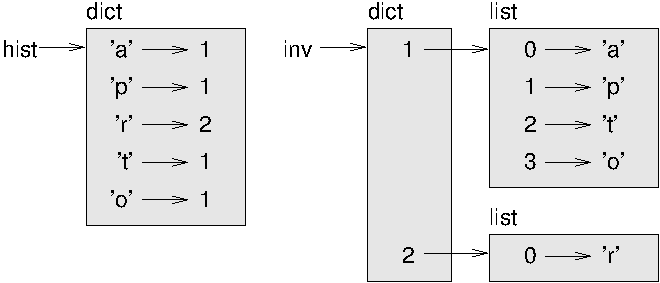
\includegraphics[scale=0.8]{figs/dict1.pdf}}
\caption{State diagram.}
\label{fig.dict1}
\end{figure}

รูป~\ref{fig.dict1} เป็นแผนภาพสถานะ ที่แสดง \texttt{hist} และ \texttt{inverse}.
%
ดิกชันนารี แสดงด้วยกล่องที่มีชนิด \texttt{dict} อยู่ข้างบน
และมี\textit{คู่กุญแจ-ค่า}เป็นคู่ ๆ อยู่ข้างใน.
ถ้าค่าเป็นเลขจำนวนเต็ม เลขทศนิยม หรือสายอักขระ มันจะวาดอยู่ในกล่อง
แต่ถ้าเป็นลิสต์ อาจจะวาดอยู่นอกกล่อง เพื่อให้แผนภาพดูง่าย.
\index{แผนภาพสถานะ}
\index{state diagram}
\index{diagram!state}

ลิสต์สามารถเป็นค่าในดิกชันนารีได้ เช่นที่แสดงในตัวอย่างนี้
แต่ลิสต์ไม่สามารถใช้เป็นกุญแจได้.
ข้างล่างนี้เป็นตัวอย่างว่าจะเกิดอะไรขึ้น ถ้าเราลอง:
\index{TypeError}
\index{exception!TypeError}


\begin{verbatim}
>>> t = [1, 2, 3]
>>> d = dict()
>>> d[t] = 'oops'
Traceback (most recent call last):
  File "<stdin>", line 1, in ?
TypeError: list objects are unhashable
\end{verbatim}
%
ตามที่ได้บอกไว้ตอนต้นว่า ดิกชันนารีถูกสร้างขึ้นมาด้วยตารางแฮช (hashtable)
และนั่นหมายถึงว่า กุญแจต่าง ๆ ต้อง\textbf{สามารถทำแฮชได้} (\textbf{hashable}).
%I mentioned earlier that a dictionary is implemented using
%a hashtable and that means that the keys have to be {\bf hashable}.
\index{ฟังก์ชันแฮช}
\index{ตารางแฮช}
\index{hash function}
\index{hashable}

\textbf{แฮช} (\textbf{hash}) เป็นฟังก์ชันที่รับค่า (ของชนิดข้อมูลใด ๆ) และรีเทิร์นค่าเลขจำนวนเต็มออกมา.
ดิกชันนารีให้ค่าเลขจำนวนเต็มต่าง ๆ ที่ได้นี้ ซึ่งเรียกว่า ค่าแฮช (hash values)
เพื่อเก็บและค้นหา\textit{คู่กุญแจค่า}ของดิกต์.
\index{immutability}

ระบบนี้ทำงานได้อย่างดี ถ้ากุญแจต่าง ๆ ไม่สามารถถูกเปลี่ยนแปลงได้.
แต่ถ้ากุญแจต่าง ๆ เปลี่ยนได้ แบบเดียวกับลิสต์ ปัญหาจะเกิดขึ้น.
ตัวอย่างเช่น ถ้าเราสร้างคู่กุญแจค่า
ไพธอนจะทำแฮชกุญแจ และเก็บค่าของกุญแจตามตำแหน่งที่แฮชได้.
ถ้าเราไปเปลี่ยนกุญแจ เมื่อทำแฮช มันจะวิ่งไปหาที่ตำแหน่งอื่น.
ในกรณีนั้น เราอาจจะได้ข้อมูลสองที่สำหรับกุญแจเดียวกัน
หรือเราอาจจะไม่สามารถหากุญแจได้เลย.
ไม่ว่าอย่างไร ดิกชันนารีจะทำงานผิดพลาด.

นั่นจึงเป็นเหตุผลที่กุญแจต่าง ๆ ต้องสามารถทำแฮชได้ และทำไมชนิดข้อมูลที่เปลี่ยนแปลงได้  เช่น ลิสต์ถึงไม่สามารถทำแฮชได้.
วิธีง่ายที่สุดที่จะก้าวข้ามข้อจำกัดนี้ คือการใช้ ทูเพิล (tuples) ที่เราจะได้เห็นในบทต่อไป.

เนื่องจาก ตัวดิกชันนารีเองก็เป็นข้อมูลที่สามารถเปลี่ยนแปลงได้
มันจึงไม่สามารถใช้เป็นกุญแจได้
แต่มัน\emph{สามารถ}ใช้เป็นค่าได้.

\section{เมโม}
\label{memoize}

ตอนที่เราลองเล่นกับฟังก์ชัน \texttt{fibonacci} ในหัวข้อ~~\ref{one.more.example}
สังเกตว่า ยิ่งเราใส่ค่าอาร์กิวเมนต์ใหญ่เท่าไร 
ฟังก์ชันยิ่งใช้เวลารันนานเท่านั้น.
%
นอกจากนั้น สังเกตว่าเวลารันเพิ่มขึ้นเร็วมาก.
\index{fibonacci function}
\index{function!fibonacci}
\index{ฟังก์ชันฟีโบนัชชี}
\index{ฟังก์ชัน!ฟีโบนัชชี}

เพื่อดูว่าทำไมจึงเป็นเช่นนั้น
ดูรูป~~\ref{fig.fibonacci} ที่แสดง \textbf{กราฟการเรียกใช้} (\textbf{call graph}) สำหรับ \texttt{fibonacci} ที่ใช้ \texttt{n=4}:
%To understand why, consider Figure~\ref{fig.fibonacci}, which shows
%the {\bf call graph} for {\tt fibonacci} with {\tt n=4}:

\begin{figure}
\centerline
{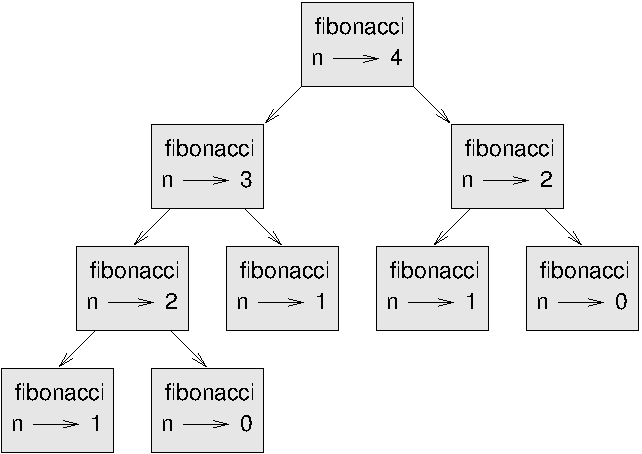
\includegraphics[scale=0.7]{figs/fibonacci.pdf}}
\caption{กราฟการเรียกใช้ (Call graph).}
\label{fig.fibonacci}
\end{figure}

กราฟการเรียกใช้แสดงฟังก์ชัน พร้อมลูกศรเชื่อมฟังก์ชันที่เรียกกับฟังก์ชันที่ถูกเรียก.
บนสุดของกราฟ \texttt{fibonacci} กับ \texttt{n=4} เรียก
\texttt{fibonacci} กับ \texttt{n=3} และกับ \texttt{n=2}.  
ในทำนองเดียวกัน \texttt{fibonacci} กับ \texttt{n=3} เรียก
\texttt{fibonacci} กับ \texttt{n=2} และกับ \texttt{n=1}.  
และต่อ ๆ ไปแบบเดียวกัน.
\index{function frame}
\index{frame}
\index{call graph}
\index{กราฟการเรียกใช้}

ถ้านับจำนวนครั้งที่ \texttt{fibonacci(0)} และ \texttt{fibonacci(1)} ถูกเรียกใช้
จะพบว่า นี่เป็นวิธีที่ไม่มีประสิทธิภาพ และมันจะยิ่งแย่ถ้าค่าอาร์กิวเมนต์ใหญ่ขึ้น.
\index{memo}
\index{เมโม}

วิธีแก้ปัญหา คือ เก็บค่าที่ได้คำนวณแล้วไว้ในดิกชันนารี.
ค่าที่ได้เคยคำนวณไว้แล้วและเก็บไว้ใช้ภายหลังจะเรียกว่า \textbf{เมโม} (\textbf{memo}).
ข้างล่างนี้คือเวอร์ชั่นที่ทำเมโมของ \texttt{fibonacci}:

\begin{verbatim}
known = {0:0, 1:1}

def fibonacci(n):
    if n in known:
        return known[n]

    res = fibonacci(n-1) + fibonacci(n-2)
    known[n] = res
    return res
\end{verbatim}
%
ตัวแปร \texttt{known} เป็นดิกชันนารีที่เก็บค่าของเลขฟีโบนัชชี ที่ได้คำนวณไว้แล้ว.
มันเริ่มจากสองรายการ: กุญแจ 0 ไปหาค่า 0 และกุญแจ 1 ไปหาค่า 1.

เมื่อไรที่ \texttt{fibonacci} ถูกเรียก
มันจะดู \texttt{known}.
ถ้าผลที่ต้องการมีอยู่แล้วในตัวแปร \texttt{known}
\texttt{fibonacci} สามารถรีเทิร์นค่าออกนั้นออกมาได้เลย.
หรือถ้าผลที่ต้องการยังไม่มี ก็คำนวณผลออกมา และเก็บไว้ในดิกชันนารี แล้วค่อยรีเทิร์นค่าออกนั้นออกมา.

ถ้าลองรันเวอร์ชั่นนี้ของ \texttt{fibonacci} และเปรียบเทียบกับเวอร์ชั่นเดิม
จะพบว่า มันเร็วกว่ามาก.

\section{ตัวแปรส่วนกลาง}
\index{global variable}
\index{variable!global}
\index{ตัวแปรส่วนกลาง}

ตัวอย่างที่แล้ว ตัวแปร \texttt{known} ถูกสร้างอยู่นอกฟังก์ชัน
ดังนั้นมันจะอยู่ภายใต้ขอบเขตพิเศษ เรียกว่า \verb"__main__".
ตัวแปรต่าง ๆ ที่อยู่ภายใต้ขอบเขต \verb"__main__" บางครั้งจะเรียกว่า \textbf{เป็นส่วนกลาง} (\textbf{global})
เพราะว่าตัวแปรเหล่านี้สามารถถูกเข้าถึงได้จากทุก ๆ ฟังก์ชัน.
ต่างจากตัวแปรเฉพาะที่ ซึ่งจะหายไปเมื่อฟังก์ชันจบ
ตัวแปรส่วนกลางจะคงอยู่ได้ ผ่านการเรียกใช้แต่ละครั้ง.
\index{flag}
\index{main}

ตัวแปรส่วนกลางนิยมใช้สำหรับเป็น \textbf{ตัวบ่งชี้} (\textbf{flags});
นั่นคือ ตัวแปรบูลีนต่าง ๆ ที่ใช้บอกสถานะ (แบบเดียวกับ ธง) ว่าสถานะเป็นจริงหรือเปล่า.
ตัวอย่างเช่น บางโปรแกรมใช้ตัวบ่งชี้ ชื่อ \texttt{verbose} เพื่อใช้บอกระดับความละเอียดของเอาต์พุต:

\begin{verbatim}
verbose = True

def example1():
    if verbose:
        print('Running example1')
\end{verbatim}
%
ถ้าลองกำหนดค่าใหม่ให้กับตัวแปรส่วนกลางดู
เราจะฉงนได้.
ตัวอย่างต่อไปนี้พยายามที่จะเก็บบันทึกว่าฟังก์ชันถูกเรียกใช้แล้วหรือไม่:
\index{reassignment}

\begin{verbatim}
been_called = False

def example2():
    been_called = True         # WRONG
\end{verbatim}
%
พอเรารันโปรแกรมนี้ดู เราจะเห็นว่าค่า \verb"been_called"
ไม่ได้เปลี่ยนไปเลย.  
ปัญหาคือ \texttt{example2} สร้างตัวแปรเฉพาะที่ใหม่ขึ้นมา ชื่อ \verb"been_called".  
ตัวแปรเฉพาะที่หายไป ตอนฟังก์ชันจบ
และไม่ได้มีผลอะไรกับตัวแปรส่วนกลาง.
\index{global statement}
\index{statement!global}
\index{declaration}

ถ้าจะกำหนดค่าใหม่ให้กับตัวแปรส่วนกลางจากภายในฟังก์ชัน
เราต้อง\textbf{ประกาศ}ตัวแปรส่วนกลาง ก่อนที่จะใช้มัน:

\begin{verbatim}
been_called = False

def example2():
    global been_called 
    been_called = True
\end{verbatim}
%
คำสั่ง \texttt{global} บอกอินเตอร์พรีเตอร์ ทำนองว่า
``ในฟังก์ชันนี้ ถ้าเราพูดว่า \verb"been_called"
เราหมายถึงตัวแปรส่วนกลาง ไม่ต้องสร้างตัวแปรเฉพาะที่ขึ้นมาใหม่.''
\index{update!global variable}
\index{global variable!update}
\index{ตัวแปรส่วนกลาง}

นี่เป็นตัวอย่างที่พยายามกำหนดค่าให้กับตัวแปรส่วนกลาง:

\begin{verbatim}
count = 0

def example3():
    count = count + 1          # WRONG
\end{verbatim}
%
ถ้ารันไป เราจะได้:
\index{UnboundLocalError}
\index{exception!UnboundLocalError}

\begin{verbatim}
UnboundLocalError: local variable 'count' referenced before assignment
\end{verbatim}
%
ไพธอนจะคิดว่า \texttt{count} เป็นตัวแปรเฉพาะที่
และเข้าใจว่า เราพยายามจะใช้ค่าของมัน ก่อนกำหนดค่าให้มัน.
วิธีแก้ไขก็แบบเดิม คือ ประกาศ \texttt{count} เป็นตัวแปรส่วนกลาง.
\index{counter}

\begin{verbatim}
def example3():
    global count
    count += 1
\end{verbatim}
%
ถ้าตัวแปรส่วนกลางอ้างถึง ค่าข้อมูลที่สามารถเปลี่ยนแปลงได้ (mutable value)
เราสามารถแก้ไขค่านั้นได้เลย โดยไม่ต้องประกาศตัวแปร:
\index{mutability}

\begin{verbatim}
known = {0:0, 1:1}

def example4():
    known[2] = 1
\end{verbatim}
%
ดังนั้น เราสามารถเพิ่ม ลบ แก้ไข ค่าของลิสต์ส่วนกลาง หรือดิกชันนารีส่วนกลางได้
แต่ถ้าเราต้องการกำหนดค่าข้อมูลใหม่ให้กับตัวแปร เราต้องประกาศให้ชัดเจน:

\begin{verbatim}
def example5():
    global known
    known = dict()
\end{verbatim}
%
ตัวแปรส่วนกลางนั้นนับว่ามีประโยชน์อยู่
แต่ถ้าเรามีตัวแปรส่วนกลางมากเกินไป
และเราแก้ไขค่าข้อมูลของมันบ่อยเกินไป
มันก็อาจจะทำให้โปรแกรมดีบักได้ยาก.


\section{การดีบัก}
\index{debugging}
\index{การดีบัก}

ตอนที่เราทำงานกับชุดข้อมูลที่ใหญ่ ๆ 
มันอาจจะไม่ค่อยสะดวก
ที่จะดีบักด้วยการพิมพ์ออกหน้าจอ และค่อย ๆ ไล่ตรวจสอบผลลัพธ์ด้วยตา
%As you work with bigger datasets it can become unwieldy to
%debug by printing and checking the output by hand.  
ข้างล่างนี้เป็นคำแนะนำสำหรับการดีบักชุดข้อมูลขนาดใหญ่:
%Here are some suggestions for debugging large datasets:

\begin{description}

\item[ปรับขนาดของอินพุตลง:] 
ถ้าทำได้ ให้ลดขนาดของชุดข้อมูลลง.
ตัวอย่างเช่น ถ้าโปรแกรมอ่านไฟล์ข้อความ
ให้เริ่มจาก 10 บรรทัดแรกก่อน หรือเริ่มจากตัวอย่างบางส่วนที่เล็กที่สุดที่จะหาได้ก่อน.
%If possible, reduce the size of the
%dataset.  For example if the program reads a text file, start with
%just the first 10 lines, or with the smallest example you can find.
อาจจะเข้าไปแก้ไขไฟล์โดยตรงเลย หรือ(ดีกว่า) อาจจะเข้าไปแก้ไขโปรแกรม ให้มันอ่านเฉพาะ \texttt{n} บรรทัดแรก ๆ ก่อน. 

ถ้ามีข้อผิดพลาดอยู่ อาจจะลองลด \texttt{n} ลงให้เป็นค่าเล็กที่สุด เท่าที่ยังมองเห็นปัญหาได้อยู่
แล้วค่อยเพิ่มมันทีละขั้น ๆ ตอนที่เจอและแก้ไขปัญหาได้.

\item[ตรวจสอบสรุปและชนิดข้อมูล:] 
แทนที่จะพิมพ์ข้อมูลทั้งหมดออกหน้าจอ และไล่ตรวจสอบรายละเอียดทั้งหมดด้วยตา
%Instead of printing and checking the
%entire dataset, 
อาจจะลองพิมพ์เฉพาะสรุปข้อมูลออกหน้าจอ: ตัวอย่างเช่น
%consider printing summaries of the data: for example,
จำนวนรายการในดิกชันนารี หรือจำนวนรายการของลิสต์.
%the number of items in a dictionary or the total of a list of numbers.

สาเหตุหนึ่งที่พบบ่อยมาก ๆ สำหรับข้อผิดพลาดเวลาดำเนินการ (runtime errors) คือ ค่าข้อมูลไม่ใช่ชนิดข้อมูลที่ถูกต้อง.
%A common cause of runtime errors is a value that is not the right
type.  
การดีบักข้อผิดพลาดแบบนี้ ก็แค่พิมพ์ชนิดของค่าข้อมูลออกมาหน้าจอเท่านั้น.
%For debugging this kind of error, it is often enough to print
%the type of a value.

\item[เขียนโปรแกรมให้มีการตรวจสอบตัวเอง:]  
บางครั้ง เราอาจจะเขียนโปรแกรมให้ตรวจสอบข้อผิดพลาดโดยอัตโนมัติไว้เลย.
ตัวอย่างเช่น ถ้าเราคำนวณค่าเฉลี่ยของลิสต์ของตัวเลข
เราอาจจะตรวจสอบว่า ผลลัพธ์ที่ได้ไม่ใหญ่กว่าค่าในลิสต์ที่ใหญ่ที่สุด และผลลัพธ์ที่ได้ไม่เล็กกว่าค่าในลิสต์ที่เล็กที่สุด.
การทำแบบนี้ เขาเรียกว่า ``เซนิตี้เช็ค'' (sanity check) หรือตรวจสอบว่ายังไม่บ้า
เพราะว่า โปรแกรมมันตรวจหาผลที่มันดู``บ้า ๆ'' (insane).
\index{sanity check}
\index{consistency check}

การตรวจสอบอีกแบบหนึ่งที่เปรียบเทียบผลการคำนวณสองวิธีที่แตกต่างกัน เพื่อดูว่าผลที่ได้สอดคล้องกันหรือไม่.
แบบนี้จะเรียกว่า ``การตรวจสอบความสอดคล้อง'' (consistency check).

\item[จัดรูปแบบของเอาต์พุต:] การจัดรูปแบบของผลแสดงจากการดีบัก จะช่วยให้มองเห็นข้อผิดพลาดได้ง่ายขึ้น.
เราได้เห็นตัวอย่างไปแล้วในหัวข้อ~\ref{factdebug}.  
เครื่องมืออีกตัวที่อาจจะมีประโยชน์ คือ โมดูล \texttt{pprint} ที่มีฟังก์ชัน \texttt{pprint} ซึ่งสามารถแสดงชนิดข้อมูลในตัว (built-in types) ในรูปแบบที่ช่วยให้มนุษย์อ่านได้ง่ายขึ้น
(\texttt{pprint} ย่อจาก ``pretty print'').
%Another tool you might find useful is the {\tt pprint} module, which provides
%a {\tt pprint} function that displays built-in types in
%a more human-readable format ({\tt pprint} stands for
%``pretty print'').
\index{pretty print}
\index{pprint module}
\index{module!pprint}

\end{description}

ย้ำอีกครั้ง เวลาที่เราทำโครงโปรแกรมสามารถช่วยลดเวลาที่เราให้ดีบักโปรแกรม.
\index{scaffolding}


\section{อภิธานศัพท์}

\begin{description}

\item[การแปลง (mapping):] ความสัมพันธ์ ที่แต่ละรายการในเซ็ตหนึ่ง คู่กันกับรายการในอีกเซ็ตหนึ่ง
%A relationship in which each element of one set
%corresponds to an element of another set.
\index{mapping}
\index{การแปลง}

\item[ดิกชันนารี (dictionary):] 
การแปลงจากกุญแจ (keys) ไปหาค่าของมัน (values).
%A mapping from keys to their
%corresponding values.
\index{dictionary}
\index{ดิกชันนารี}

\item[คู่กุญแจค่า (key-value pair):] 
คู่ของการแปลงจากกุญแจหนึ่งไปหาค่าของมัน
%The representation of the mapping from
%a key to a value.
\index{key-value pair}
\index{คู่กุญแจค่า}

\item[ค่ารายการ (item):] สำหรับดิกชันนารี ค่ารายการ หมายถึง คู่กุญแจค่า.
\index{item!dictionary}

\item[กุญแจ (key):] เป็นสิ่งที่อยู่ในดิกชันนารี ที่ปรากฎเป็นส่วนแรกของคู่กุญแจค่า.
\index{key}

\item[ค่า (value):] เป็นสิ่งที่อยู่ในดิกชันนารี ที่ปรากฎเป็นส่วนหลังของคู่กุญแจค่า.
ความหมายนี้จะเจาะจงมากกว่าความหมายทั่วไปของคำว่า ``ค่า'' (value).
\index{value}

\item[อิมพลิเมนเตชั่น (implementation):] เป็นวิธีที่ใช้ทำการคำนวณ.
\index{implementation}

\item[ตารางแฮช (hashtable):] อัลกอริทึมที่ใช้ทำการคำนวณสำหรับดิกชันนารี.
\index{hashtable}

\item[ฟังก์ชันแฮช (hash function):] ฟังก์ชันที่ใช้ตารางแฮช เพื่อคำนวณตำแหน่งของกุญแจ.
\index{hash function}

\item[สามารถทำแฮชได้ (hashable):] ชนิดข้อมูลที่มีฟังก์ชันแฮชอยู่.  
ชนิดข้อมูลที่เปลี่ยนแปลงไม่ได้ (immutable types) เช่น
จำนวนเต็ม (integers)
เลขทศนิยม (floats)
และ สายอักขระ (strings) สามารถทำแฮชได้.
ชนิดข้อมูลที่เปลี่ยนแปลงได้ (mutable types) เช่น ลิสต์ (lists) และ
ดิกชันนารี (dictionaries) ไม่สามารถทำแฮชได้.
\index{hashable}

\item[การเทียบค้น (lookup):] ปฏิบัติการของดิกชันนารีที่รับกุญแจเข้าไป และค้นหาค่าของกุญแจนั้นออกมา.
\index{lookup}

\item[การเทียบค้นย้อนกลับ (reverse lookup):] ปฏิบัติการของดิกชันนารีที่รับค่าเข้าไป 
และค้นหากุญแจที่เชื่อมกับค่านั้นออกมา.
\index{reverse lookup}

\item[คำสั่งเรส (raise statement):]  
คำสั่งที่(ตั้งใจ)ส่งสัญญาณเอ็กเซ็ปชั่นออกมา.
\index{raise statement}
\index{statement!raise}

\item[เซตโทน (singleton):] ลิสต์ (หรือข้อมูลลำดับชนิดอื่น) ที่มีอิลิเมนต์เดียว.
\index{singleton}

\item[กราฟการเรียกใช้ (call graph):] แผนภาพที่แสดงทุก ๆ กรอบแทนฟังก์ชัน แต่ละฟังก์ชันที่สร้างขึ้นมาระหว่างที่รันโปรแกรม โดยมีลูกศรจากส่วนที่เรียกใช้ (caller) ไปหาส่วนที่ถูกเรียกใช้ (callee). 
\index{call graph}
\index{diagram!call graph}

\item[เมโม (memo):] ค่าที่ได้คำนวณได้แล้ว และเก็บไว้เพื่อใช้ภายหลัง เพื่อไม่คำนวณซ้ำอีกในอนาคต.
\index{memo}

\item[ตัวแปรส่วนกลาง (global variable):] ตัวแปรที่นิยามอยู่นอกฟังก์ชัน.  
ตัวแปรส่วนกลางสามารถถูกเรียกใช้ได้จากทุกฟังก์ชัน.
\index{global variable}

\item[คำสั่งกำหนดตัวแปรส่วนกลาง (global statement):]  คำสั่งที่กำหนดให้ตัวแปรเป็นตัวแปรส่วนกลาง
\index{global statement}
\index{statement!global}

\item[ตัวบ่งชี้ (flag):] ตัวแปรบูลีนที่ใช้ระบุว่าเงื่อนไขเป็นจริงหรือไม่.
\index{flag}

\item[การประกาศ (declaration):] คำสั่ง เช่นพวก \texttt{global} ที่บอกอินเตอร์พรีเตอร์บางอย่างเกี่ยวกับตัวแปร.
\index{declaration}

\end{description}


\section{แบบฝึกหัด}

\begin{exercise}
\label{wordlist2}
\index{set membership}
\index{membership!set}

เขียนฟังก์ชันที่อ่านคำใน \texttt{words.txt} และเก็บคำเหล่านั้นเป็นกุญแจของดิกชันนารี.  
มันไม่สำคัญว่าค่าของกุญแจเป็นเท่าไร.
เราสามารถใช้ตัวปฏิบัติการ \texttt{in} เป็นวิธีที่รวดเร็วในการตรวจสอบว่าคำที่สนใจมีอยู่ในดิกชันนารีหรือไม่.

ถ้าทำแบบฝึกหัด~\ref{wordlist1}มาแล้ว เราสามารถเปรียบเทียบความเร็วของอิมพลิเมนเตชั่นนี้ กับลิสต์ที่ใช้ \texttt{in} และวิธีค้นหาแบบแบ่งสอง (bisection search).

\end{exercise}
\vspace{0.5cm}


\begin{exercise}
\label{setdefault}

อ่านเอกสารประกอบของดิกชันนารีเมธอด \texttt{setdefault}
และใช้เมธอดนี้เพื่อเขียนโปรแกรมในแบบที่กระชับขึ้นของ \verb|invert_dict|.
เฉลย: \url{http://thinkpython2.com/code/invert_dict.py}.
\index{setdefault method}
\index{method!setdefault}

\end{exercise}
\vspace{0.5cm}


\begin{exercise}
ใช้เมโม เพื่อทำฟังก์ชันแอกเคอมันน์ (Ackermann function) จากแบบฝึกหัด~\ref{ackermann} 
และดูว่า การใช้เมโม ช่วยให้สามารถรันฟังก์ชัน เมื่อใช้กับอาร์กิวเมนต์ที่ใหญ่ขึ้นได้หรือไม่.  
คำใบ้: ไม่ได้.
เฉลย: \url{http://thinkpython2.com/code/ackermann_memo.py}.
\index{Ackermann function}
\index{function!ack}

\end{exercise}
\vspace{0.5cm}



\begin{exercise}
\index{duplicate}

จากแบบฝึกหัด~\ref{duplicate} เราจะมีฟังก์ชันชื่อ \verb|has_duplicates| ที่รับลิสต์เป็นพารามิเตอร์ และรีเทิร์น \texttt{True} ออกมา ถ้ามีรายการที่ซ้ำอยู่ในลิสต์.

ใช้ดิกชันนารีเพื่อเขียนโปรแกรมแบบที่เร็วขึ้นและง่ายขึ้นของฟังก์ชัน
\verb|has_duplicates|. 
เฉลย: \url{http://thinkpython2.com/code/has_duplicates.py}.

\end{exercise}
\vspace{0.5cm}


\begin{exercise}
\label{exrotatepairs}
\index{letter rotation}
\index{rotation!letters}

คำสองคำเรียกว่าเป็น ``คู่หมุนเปลี่ยน'' (rotate pair) 
เมื่อเราหมุนคำหนึ่งและผลลัพธ์ได้เป็นอีกคำหนึ่ง (ดู \verb|rotate_word| ใน แบบฝึกหัด~\ref{exrotate}).

เขียนโปรแกรมที่อ่านลิสต์ของคำ และหาคู่หมุนเปลี่ยนออกมาทั้งหมด.
เฉลย: \url{http://thinkpython2.com/code/rotate_pairs.py}.

\end{exercise}
\vspace{0.5cm}


\begin{exercise}
\index{Car Talk}
\index{Puzzler}

นี่เป็นปริศนาจาก \textbf{Car Talk} 
(\url{http://www.cartalk.com/content/puzzlers}):

\begin{quote}
เรื่องนี้ส่งมาจากสหายชื่อว่า แดน โอเลียรี่.
แดนฉงนกับคำพยางค์เดียวห้าอักษร ที่มีคุณสมบัติพิเศษ.
นั่นคือ เมื่อเราเอาอักษรแรกออก ตัวอักษรที่เหลือจะเป็นคำพ้องเสียง (homophone) ของคำเดิม นั่นคือคำใหม่จะออกเสียงเหมือนเดิมเลย.
แถมถ้าไม่เอาอักษรตัวแรกออก แต่เอาอักษรตัวที่สองออก
ผลก็ยังเป็นคำพ้องเสียงเดิมอยู่.
คำถามคือ คำนั้นคือคำอะไร

เดี๋ยวผมจะให้ตัวอย่างคำที่ไม่ใช่. 
ลองคำว่า `wrack' W-R-A-C-K ก็แบบที่รู้ เช่น `wrack with
pain.' 
ถ้าผมเอาอักษรตัวแรกออก ผมจะเหลือแค่ 'R-A-C-K' เหมือนที่คำพูด `Holy cow, did you see the rack on that buck!'
เกือบได้แล้ว 
เพียงแต่เมื่อเราใส่ `w' กลับเข้าไป แต่เอา `r' ออกแทน
เราจะได้ `wack' ซึ่งไม่ได้พ้องเสียงกับอีกสองคำ (`wrack' และ `rack')

แต่มันมีอย่างน้อยก็คำหนึ่งหละ ที่แดนและเรารู้ว่าจะให้คำพ้องเสียงสองคำออกมา 
ไม่ว่าจะเอาอักษรตัวแรก หรือตัวที่สองออก คำถามคือคำนั้นคือคำว่าอะไร
\end{quote}
\index{homophone}
\index{reducible word}
\index{word, reducible}

เราสามารถใช้ดิกชันนารีจากแบบฝึกหัด~\ref{wordlist2} 
เพื่อตรวจสอบว่าสายอักขระอยู่ในลิสต์ของคำหรือไม่.
เพื่อตรวจสอบว่าคำสองคำเป็นคำพ้องเสียงหรือไม่
เราสามารถใช้พจนานุกรมการออกเสียงซีเอ็มยู (CMU
Pronouncing Dictionary)
ซึ่งสามารถดาวน์โหลดได้จาก
\url{http://www.speech.cs.cmu.edu/cgi-bin/cmudict} 
หรือจาก
\url{http://thinkpython2.com/code/c06d} 
และยังสามารถดาวน์โหลด
\url{http://thinkpython2.com/code/pronounce.py}
ที่เตรียมฟังก์ชัน \verb"read_dictionary" ที่ใช้อ่านพจนานุกรมการออกเสียง
แล้วส่งไพธอนดิกชันนารีที่เชื่อมคำกับการออกเสียงออกมาให้.

เขียนโปรแกรมที่หาคำทั้งหมดที่ตอบปริศนานี้ออกมา
เฉลย: \url{http://thinkpython2.com/code/homophone.py}.

\end{exercise}
\vspace{0.5cm}



\chapter{ทูเพิล}
\label{tuplechap}

บทนี้นำเสนอชนิดข้อมูลสำเร็จที่มีอยู่ในตัวอีกชนิดหนึ่ง ซึ่งคือ ทูเพิล
พร้อมแสดงวิธีการใช้ ลิสต์ ดิกชันนารี และทูเพิล ทำงานด้วยกัน.
%
%I also present a useful feature for variable-length argument lists,
%the gather and scatter operators.
%
นอกจากนั้น เรายังอภิปรายกันถึง
คุณลักษณะที่มีประโยชน์ของอาร์กิวเมนต์ความยาวแปรผัน
พร้อมตัวดำเนินการ\textit{การรวบรวม}และ\textit{การกระจาย}. 

%One note: there is no consensus on how to pronounce ``tuple''.
%Some people say ``tuh-ple'', which rhymes with ``supple''.  But
%in the context of programming, most people say ``too-ple'', which
%rhymes with ``quadruple''.

เรื่องหนึ่ง: ยังไม่มีข้อตกลงอย่างเป็นทางการว่า ควรจะอ่าน ``tuple'' อย่างไร.
บางคนอ่าน ``ทับ-เพิล'' ที่คล้องกับ ``supple''.
แต่ในบริบทของการเขียนโปรแกรม คนส่วนใหญ่อ่าน ``ทู-เพิล'' ที่คล้องกับ ``quadruple''.


%\section{Tuples are immutable}
\section{ทูเพิลไม่สามารถเปลี่ยนแปลงได้}
\index{tuple}
\index{type!tuple}
\index{sequence}
\index{ทูเพิล}
\index{ชนิดข้อมูล!ทูเพิล}

%A tuple is a sequence of values.  The values can be any type, and
%they are indexed by integers, so in that respect tuples are a lot
%like lists.  The important difference is that tuples are immutable.

ทูเพิลเป็นลำดับของค่าต่าง ๆ.
ค่าต่าง ๆ เป็นข้อมูลชนิดใดก็ได้
และค่าต่าง ๆ เหล่านั้นอ้างอิงได้ด้วยดัชนีที่เป็นเลขจำนวนเต็ม
ซึ่งในแง่นี้ ทูเพิลจะคล้าย ๆ กับลิสต์.
ความต่างที่สำคัญเลย คือ ทูเพิลไม่สามารถเปลี่ยนแปลงแก้ไขได้.
\index{mutability}
\index{immutability}
\index{ความสามารถในการเปลี่ยนแปลงได้}
\index{ความไม่สามารถในการเปลี่ยนแปลงได้}

%Syntactically, a tuple is a comma-separated list of values:

ในแง่ไวยากรณ์ ทูเพิล เป็นลำดับของค่าต่าง ๆ ที่คั่นระหว่างกันด้วยเครื่องหมายจุลภาค (`,') เช่น

\begin{verbatim}
>>> t = 'a', 'b', 'c', 'd', 'e'
\end{verbatim}
%
%Although it is not necessary, it is common to enclose tuples in
%parentheses:

นอกจากนั้น ทูเพิลมักจะอยู่ระหว่างเครื่องหมายวงเล็บ
ซึ่งจริง ๆ แล้ว มันไม่ได้จำเป็นเลย ที่จะต้องใช้เครื่องหมายวงเล็บ เช่น
\index{parentheses!tuples in}

\begin{verbatim}
>>> t = ('a', 'b', 'c', 'd', 'e')
\end{verbatim}
%
%To create a tuple with a single element, you have to include a final
%comma:

เพื่อสร้างทูเพิลที่มีอิลิเมนต์เดียว เราจำเป็นถ้าใส่เครื่องจุลภาคต่อท้ายเข้าไป
เช่น
\index{singleton}
\index{tuple!singleton}
\index{เซตโทน}
\index{ทูเพิล!เซตโทน}

\begin{verbatim}
>>> t1 = 'a',
>>> type(t1)
<class 'tuple'>
\end{verbatim}
%
%A value in parentheses is not a tuple:
ค่าในวงเล็บไม่ใช่ทูเพิล:

\begin{verbatim}
>>> t2 = ('a')
>>> type(t2)
<class 'str'>
\end{verbatim}
%
%Another way to create a tuple is the built-in function {\tt tuple}.
%With no argument, it creates an empty tuple:

อีกวิธีที่จะสร้างทูเพิล คือ การใช้ฟังก์ชันสำเร็จที่มีอยู่ในตัว \texttt{tuple}.
ถ้าไม่ใส่อาร์กิวเมนต์  มันจะสร้างทูเพิลว่างให้:
\index{tuple function}
\index{function!tuple}
\index{ฟังก์ชัน!tuple}

\begin{verbatim}
>>> t = tuple()
>>> t
()
\end{verbatim}
%
%If the argument is a sequence (string, list or tuple), the result
%is a tuple with the elements of the sequence:

ถ้าอาร์กิวเมนต์ของฟังก์ชัน เป็นลำดับ (ไม่ว่าจะเป็น สายอักขระ ลิสต์ หรือทูเพิล)
ผลที่ได้จะเป็น ทูเพิลของอิลิเมนต์ของลำดับนั้น:

\begin{verbatim}
>>> t = tuple('lupins')
>>> t
('l', 'u', 'p', 'i', 'n', 's')
\end{verbatim}
%
%Because {\tt tuple} is the name of a built-in function, you should
%avoid using it as a variable name.

เพราะว่า \texttt{tuple} เป็นชื่อของฟังก์ชันสำเร็จรูป
เราจึงไม่ควรใช้มันเป็นชื่อตัวแปร.

%Most list operators also work on tuples.  The bracket operator
%indexes an element:

ตัวดำเนินการต่าง ๆ ที่ใช้กับลิสต์ได้ ส่วนใหญ่ก็ใช้กับทูเพิลได้.
ตัวดำเนินการวงเล็บสี่เหลี่ยมเลือกอิลิเมนต์ตามดัชนี:
\index{bracket operator}
\index{operator!bracket}
\index{ตัวดำเนินการวงเล็บสี่เหลี่ยม}
\index{ตัวดำเนินการ!วงเล็บสี่เหลี่ยม}

\begin{verbatim}
>>> t = ('a', 'b', 'c', 'd', 'e')
>>> t[0]
'a'
\end{verbatim}
%
%And the slice operator selects a range of elements.
%
และตัวดำเนินการตัด (slice operator) เลือกขอบเขตของอิลิเมนต์ เช่น
\index{slice operator}
\index{operator!slice}
\index{tuple!slice}
\index{slice!tuple}
\index{ตัวดำเนินการตัด}
\index{ตัวดำเนินการ!การตัด}
\index{ทูเพิล!การตัดช่วง}
\index{การตัดช่วง!ทูเพิล}


\begin{verbatim}
>>> t[1:3]
('b', 'c')
\end{verbatim}
%
%But if you try to modify one of the elements of the tuple, you get
%an error:
%
แต่ถ้าเราลองแก้ไขค่าอิลิเมนต์ของทูเพิล เราจะเห็นข้อผิดพลาดแจ้งออกมา:
\index{exception!TypeError}
\index{TypeError}
\index{item assignment}
\index{assignment!item}

\begin{verbatim}
>>> t[0] = 'A'
TypeError: object doesn't support item assignment
\end{verbatim}
%
%Because tuples are immutable, you can't modify the elements.  But you
%can replace one tuple with another:
%
เพราะว่า ทูเพิลไม่สามารถเปลี่ยนแปลงได้ (immutable)
เราจึงไม่สามารถที่จะแก้ไข หรือเปลี่ยนแปลงอิลิเมนต์ของทูเพิลได้.
แต่เราสามารถแทนที่ทูเพิล ด้วยทูเพิลใหม่ได้:

\begin{verbatim}
>>> t = ('A',) + t[1:]
>>> t
('A', 'b', 'c', 'd', 'e')
\end{verbatim}
%
%This statement makes a new tuple and then makes {\tt t} refer to it.
คำสั่งนี้สร้างทูเพิลใหม่ขึ้นมา
และกำหนดให้ตัวแปร \texttt{t} ไปอ้างถึงมัน.

%The relational operators work with tuples and other sequences;
%Python starts by comparing the first element from each
%sequence.  If they are equal, it goes on to the next elements,
%and so on, until it finds elements that differ.  Subsequent
%elements are not considered (even if they are really big).

ตัวดำเนินการเชิงสัมพันธ์ทำงานกับทูเพิลและข้อมูลแบบลำดับชนิดอื่น ๆ ได้
ไพธอนทำงานโดย
เริ่มจากเปรียบเทียบอิลิเมนต์แรกจากแต่ละทูเพิล
ถ้าอิลิเมนต์จากสองทูเพิลเท่ากัน ไพธอนจะไม่สนใจ
และขยับไปตรวจอิลิเมนต์ในลำดับถัดไปจาอทั้งสองทูเพิล
ถ้ามันต่างกัน ไพธอนจะทำงานเปรียบเทียบ 
และใช้ผลการเปรียบเทียบของอิลิเมนต์คู่นี้ เป็นผลของตัวดำเนินการ
โดยอิลิเมนต์ที่เหลือจะไม่นำมาคิดเลย.
%
\index{comparison!tuple}
\index{tuple!comparison}
\index{การเปรียบเทียบ!ทูเพิล}
\index{ทูเพิล!การเปรียบเทียบ}

\begin{verbatim}
>>> (0, 1, 2) < (0, 3, 4)
True
>>> (0, 1, 2000000) < (0, 3, 4)
True
>>> (0, 1, 1, 8, 10, 100) < (0, 1, 1, 9, 1, 0)
True
>>> (0, 1, 1, 11, 10, 100) < (0, 1, 1, 9, 1, 0)
False
\end{verbatim}
%
คำสั่งแรก คู่แรกที่ต่างกันคือดัชนีที่ 1 และ
อิลิเมนต์ในทูเพิลแรกมีค่าน้อยกว่าอิลิเมนต์ในทูเพิลสอง (ค่า 1 เปรียบเทียบกับ 3) 
จึงให้ผลออกมาเป็น \texttt{True}.
คำสั่งสอง ก็เช่นเดียวกัน เมื่อได้ผลจากคู่ดัชนีที่ 1 (ค่า 1 เปรียบเทียบกับ 3) แล้ว
คู่ที่เหลือจะไม่ถูกคำมาคิด 
นั่นคือ คู่ดัชนี 2 (ค่า 2000000 เปรียบเทียบกับ 4) ไม่ได้ถูกนำมาคิด.
คำสั่งสาม คู่แรกที่ต่างกันคือดัชนีที่ 3 (เปรียบเทียบ ค่า 8 กับ 9)
ผลของการเปรียบเทียบคู่นี้คือ ผลลัพธ์.
คู่ที่เหลือจะไม่ถูกคำมาคิด.
คำสั่งสี่ ก็เช่นเดียวกัน เมื่อได้ผลจากคู่ดัชนี 2 (ค่า 11 เปรียบเทียบกับ 9) แล้ว
คู่ที่เหลือจะไม่ถูกคำมาคิด.

%\section{Tuple assignment}
\section{การกำหนดค่าทูเพิล}
\label{tuple.assignment}
\index{tuple!assignment}
\index{assignment!tuple}
\index{swap pattern}
\index{pattern!swap}
\index{ทูเพิล!การกำหนดค่า}
\index{การกำหนดค่า!ทูเพิล}
\index{รูปแบบการสลับค่า}
\index{รูปแบบ!การสลับค่า}

%It is often useful to swap the values of two variables.
%With conventional assignments, you have to use a temporary
%variable.  For example, to swap {\tt a} and {\tt b}:

บางครั้ง เราอาจต้องการสลับค่าระหว่างตัวแปรสองตัว.
ด้วยวิธีการกำหนดค่าแบบทั่ว ๆ ไป
เราต้องใช้ตัวแปรชั่วคราวเข้ามาช่วย.
ตัวอย่างเช่น สลับค่าระหว่างตัวแปร \texttt{a} และตัวแปร \texttt{b}:

\begin{verbatim}
>>> temp = a
>>> a = b
>>> b = temp
\end{verbatim}
%
%This solution is cumbersome; {\bf tuple assignment} is more elegant:
%
วิธีนี้ค่อนข้างงุ่มง่าม.
วิธี\textbf{การกำหนดค่าทูเพิล} (\textbf{tuple assignment}) ดูสละสลวยกว่าเยอะ:

\begin{verbatim}
>>> a, b = b, a
\end{verbatim}
%
%The left side is a tuple of variables; the right side is a tuple of
%expressions.  Each value is assigned to its respective variable.  
%All the expressions on the right side are evaluated before any
%of the assignments.
%
ฝั่งซ้ายมือเป็นทูเพิลของตัวแปร
ส่วนฝั่งขวามือเป็นทูเพิลของนิพจน์.
แต่ละค่าจะถูกกำหนดไปให้กับตัวแปรตามลำดับ.
นิพจน์ทั้งหมดทางขวามือจะถูกประเมินค่า ก่อนดำเนินการกำหนดค่า.

%The number of variables on the left and the number of
%values on the right have to be the same:

จำนวนตัวแปรทางซ้ายมือ และจำนวนของค่าต่าง ๆ ทางขวามือ จะต้องเท่ากัน:
\index{exception!ValueError}
\index{ValueError}

\begin{verbatim}
>>> a, b = 1, 2, 3
ValueError: too many values to unpack
\end{verbatim}
%
%More generally, the right side can be any kind of sequence
%(string, list or tuple).  For example, to split an email address
%into a user name and a domain, you could write:
%
จริง ๆ แล้ว ทางขวามือจะเป็นข้อมูลลำดับชนิดใด ๆ ก็ได้ (สายอักขระ ลิสต์ หรือทูเพิล).
ตัวอย่าง เช่น เพื่อจะแยกอีเมล์แอดเดรส (email address) ออกมาเป็น ชื่อผู้ใช้ และโดเมน (domain) เราอาจจะเขียน:
\index{split method}
\index{method!split}
\index{email address}

\begin{verbatim}
>>> addr = 'monty@python.org'
>>> uname, domain = addr.split('@')
\end{verbatim}
%
%The return value from {\tt split} is a list with two elements;
%the first element is assigned to {\tt uname}, the second to
%{\tt domain}.
%
ค่าที่รีเทิร์นออกมาจาก \texttt{split} เป็นลิสต์ของสองอิลิเมนต์
โดย
อิลิเมนต์แรกจะถูกกำหนดให้กับ \texttt{uname}
และอิลิเมนต์ที่สองให้กับ \texttt{domain}.

\begin{verbatim}
>>> uname
'monty'
>>> domain
'python.org'
\end{verbatim}
%

%\section{Tuples as return values}
\section{ทูเพิลที่ใช้เป็นค่าที่รีเทิร์นออกมา}
\index{tuple}
\index{value!tuple}
\index{return value!tuple}
\index{function, tuple as return value}
\index{ทูเพิล}
\index{ค่า!ทูเพิล}


%Strictly speaking, a function can only return one value, but
%if the value is a tuple, the effect is the same as returning
%multiple values.  For example, if you want to divide two integers
%and compute the quotient and remainder, it is inefficient to
%compute {\tt x/y} and then {\tt x\%y}.  It is better to compute
%them both at the same time.

ถ้าพูดกันตรง ๆ ฟังก์ชันสามารถส่งค่าออกมาได้ค่าเดียว
แต่ถ้าค่าที่ส่งออกมาเป็นทูเพิล
ผลของมันจึงเหมือนกับการส่งค่าออกมาหลาย ๆ ค่า.
ตัวอย่างเช่น ถ้าเราต้องการหารเลขจำนวนเต็ม 
และคำนวณทั้ง ผลหาร (quotient) และเศษ (remainder)
มันก็ไม่ค่อยมีประสิทธิภาพ
ถ้าต้องคำนวณ \texttt{x/y} แล้วก็ \texttt{x\%y}.
มันดีกว่าที่จะคำนวณทั้งสองอย่างพร้อม ๆ กัน.
\index{divmod}

%The built-in function {\tt divmod} takes two arguments and
%returns a tuple of two values, the quotient and remainder.
%You can store the result as a tuple:

ฟังก์ชันสำเร็จรูป \texttt{divmod} รับอาร์กิวเมนต์สองตัว
และให้ทูเพิลที่มีสองค่าออกมา
ซึ่งคือ ผลหารและเศษ.
เราสามารถเก็บค่าผลลัพธ์นี้เป็นทูเพิลได้:

\begin{verbatim}
>>> t = divmod(7, 3)
>>> t
(2, 1)
\end{verbatim}
%
%Or use tuple assignment to store the elements separately:
%
หรือ ใช้การกำหนดค่าทูเพิล เพื่อเก็บแต่ละอิลิเมนต์แยกกัน:
\index{tuple assignment}
\index{assignment!tuple}
\index{การกำหนดค่าทูเพิล}
\index{การกำหนดค่า!ทูเพิล}

\begin{verbatim}
>>> quot, rem = divmod(7, 3)
>>> quot
2
>>> rem
1
\end{verbatim}
%
%Here is an example of a function that returns a tuple:
นี่เป็นตัวอย่างของฟังก์ชันที่ให้ค่าทูเพิลออกมา:

\begin{verbatim}
def min_max(t):
    return min(t), max(t)
\end{verbatim}
%
%{\tt max} and {\tt min} are built-in functions that find
%the largest and smallest elements of a sequence.  \verb"min_max"
%computes both and returns a tuple of two values.
\texttt{max} และ \texttt{min} เป็นฟังก์ชันสำเร็จรูป
ที่ใช้หาค่ามากที่สุดและน้อยที่สุด ในข้อมูลลำดับ.
\verb|min_max| คำนวณค่าทั้งสอง และให้ทูเพิลของค่าทั้งสองออกมา.
\index{max function}
\index{function!max}
\index{min function}
\index{function!min}
\index{ฟังก์ชัน!max}
\index{ฟังก์ชัน!min}

% \section{Variable-length argument tuples}
\section{ทูเพิลที่ใช้เป็นอาร์กิวเมนต์ความยาวแปรผัน}
\label{gather}
\index{variable-length argument tuple}
\index{argument!variable-length tuple}
\index{gather}
\index{parameter!gather}
\index{argument!gather}
\index{พารามิเตอร์!รวบรวม}
\index{อาร์กิวเมนต์!รวบรวม}
\index{การรวบรวม}

%Functions can take a variable number of arguments.  
%A parameter name that begins with {\tt *} {\bf gathers} arguments into
%a tuple.  
%For example, {\tt printall}
%takes any number of arguments and prints them:

เราสามารถสร้างฟังก์ชันที่รับอาร์กิวเมนต์ที่มีจำนวนแปรเปลี่ยนได้.
ชื่อพารามิเตอร์ที่ขึ้นต้นด้วย \texttt{*} จะ\textbf{รวบรวม} (\textbf{gather}) อาร์กิวเมนต์หลาย ๆ ตัวเข้าเป็นทูเพิล.
ตัวอย่างเช่น \texttt{printall} รับอาร์กิวเมนต์กี่ตัวก็ได้ และก็พิมพ์ค่าเหล่านั้นออกมา:


\begin{verbatim}
def printall(*args):
    print(args)
\end{verbatim}
%
พารามิเตอร์รวม \texttt{args} สามารถจะตั้งเป็นชื่ออะไรก็ได้ แต่มักจะนิยมตั้งเป็นชื่อ \texttt{args}.  
ฟังก์ชันทำงานดังนี้:

\begin{verbatim}
>>> printall(1, 2.0, '3')
(1, 2.0, '3')
\end{verbatim}
%
%The complement of gather is {\bf scatter}.  If you have a
%sequence of values and you want to pass it to a function
%as multiple arguments, you can use the {\tt *} operator.
%For example, {\tt divmod} takes exactly two arguments; it
%doesn't work with a tuple:
%
ตรงข้ามกับการรวบรวมคือ \textbf{การแยกกระจาย} (\textbf{scatter}).
ถ้าเรามีค่าหลาย ๆ ค่า และต้องการส่งเข้าไปให้ฟังก์ชันผ่านอาร์กิวเมนต์หลาย ๆ ตัว
เราก็สามารถใช้ตัวดำเนินการ \texttt{*} ได้.
ตัวอย่าง \texttt{divmod} รับอาร์กิวเมนต์สองตัว ต้องการสองตัว และสองตัวเท่านั้น
ไม่ได้ใช้ทูเพิล:
%
\index{scatter}
\index{argument scatter}
\index{TypeError}
\index{exception!TypeError}
\index{parameter!scatter}
\index{argument!scatter}
\index{การแยกกระจาย}
\index{พารามิเตอร์!การแยกกระจาย}
\index{อาร์กิวเมนต์!การแยกกระจาย}


\begin{verbatim}
>>> t = (7, 3)
>>> divmod(t)
TypeError: divmod expected 2 arguments, got 1
\end{verbatim}
%
%But if you scatter the tuple, it works:
%
แต่เราสามารถแยกกระจายทูเพิลได้:

\begin{verbatim}
>>> divmod(*t)
(2, 1)
\end{verbatim}
%
%Many of the built-in functions use
%variable-length argument tuples.  For example, {\tt max}
%and {\tt min} can take any number of arguments:
%
ฟังก์ชันสำเร็จรูปหลาย ๆ อันใช้ทูเพิลเป็นอาร์กิวเมนต์ความยาวแปรผัน.
ตัวอย่างเช่น \texttt{max} และ \texttt{min} สามารถรับอาร์กิวเมนต์กี่ตัวก็ได้:

\index{max function}
\index{function!max}
\index{min function}
\index{function!min}
\index{built-in functions}
\index{ฟังก์ชันสำเร็จรูป}
\index{ฟังก์ชัน!max}
\index{ฟังก์ชัน!min}

\begin{verbatim}
>>> max(1, 2, 3)
3
\end{verbatim}
%
%But {\tt sum} does not.
แต่ \texttt{sum} ทำไม่ได้.
\index{sum function}
\index{function!sum}
\index{ฟังก์ชัน!sum}

\begin{verbatim}
>>> sum(1, 2, 3)
TypeError: sum expected at most 2 arguments, got 3
\end{verbatim}
%
%As an exercise, write a function called {\tt sumall} that takes any number
%of arguments and returns their sum.
เพื่อเป็นแบบฝึกหัด ให้ลองเขียนฟังก์ชัน ชื่อว่า \texttt{sumall} ที่รับอาร์กิวเมนต์กี่ตัวก็ได้ และรีเทิร์นค่าผลรวมออกมา.

%\section{Lists and tuples}
\section{ลิสต์และทูเพิล}
\index{zip function}
\index{function!zip}
\index{ฟังก์ชัน!zip}

%{\tt zip} is a built-in function that takes two or more sequences and
%returns a list of tuples where each tuple contains one
%element from each sequence.  The name of the function refers to
%a zipper, which joins and interleaves two rows of teeth.
%
\texttt{zip} เป็นฟังก์ชันสำเร็จรูป ที่รับข้อมูลลำดับตั้งแต่สองชุดขึ้นไป
และรีเทิร์นลิสต์ของทูเพิลออกมา
โดยที่ แต่ละทูเพิล จะมีอิลิเมนต์มาจากแต่ละชุดข้อมูลลำดับ.
ชื่อของฟังก์ชันมาจาก ซิป(ซิปกางเกง) 
ที่รูดแล้ว มันจะขบฟันของซิปจากสองฝั่งเข้าด้วยกัน.

%This example zips a string and a list:
%
ตัวอย่างนี้ซิปข้อมูลสายอักขระและลิสต์เข้าด้วยกัน
\begin{verbatim}
>>> s = 'abc'
>>> t = [0, 1, 2]
>>> zip(s, t)
<zip object at 0x7f7d0a9e7c48>
\end{verbatim}
%
%The result is a {\bf zip object} that knows how to iterate through the pairs.  The most common use of {\tt zip} is in a {\tt for} loop:
%
ผลลัพธ์จากฟังก์ชัน \texttt{zip} จะเป็น \textbf{ซิปออบเจ๊คต์} (\textbf{zip object})
ที่สามารถวนเข้าถึงแต่ละคู่ทูเพิลได้.
วิธีที่นิยมใช้กับ \texttt{zip} ที่สุดคือ ใช้กับลูป \texttt{for} เช่น:

\begin{verbatim}
>>> for pair in zip(s, t):
...     print(pair)
...
('a', 0)
('b', 1)
('c', 2)
\end{verbatim}
%
%A zip object is a kind of {\bf iterator}, 
%which is any object
%that iterates through a sequence.  Iterators are similar to lists in some
%ways, but unlike lists, you can't use an index to select an element from an iterator.
%
ซิปออบเจ๊คต์ เป็น \textbf{ตัววนซ้ำ} (\textbf{iterator})
ซึ่งเป็นออบเจ๊คต์ที่สามารถทำวนซ้ำกับลำดับได้.
ตัววนซ้ำ จะคล้าย ๆ กับลิสต์ ในหลาย ๆ แง่
แต่ต่างจากลิสต์ คือ เราไม่สามารถใช้ดัชนีเลือกอิลิเมนต์ออกมาจากตัววนซ้ำได้.
%
\index{iterator}
\index{ตัววนซ้ำ}


%If you want to use list operators and methods, you can
%use a zip object to make a list:
%
ถ้าต้องการใช้ตัวดำเนินการของลิสต์จริง ๆ
เราก็สามารถแปลงซิปออปเจ๊คต์ไปเป็นลิสต์ได้:

\begin{verbatim}
>>> list(zip(s, t))
[('a', 0), ('b', 1), ('c', 2)]
\end{verbatim}
%
%The result is a list of tuples; in this example, each tuple contains
%a character from the string and the corresponding element from the list.
%
ผลลัพธ์จะเป็นลิสต์ของทูเพิล
ในตัวอย่างนี้ แต่ละทูเพิลจะมีอักขระจากสายอักขระ \texttt{s}
และอิลิเมนต์จากลิสต์ \texttt{t}.
%
\index{list!of tuples}

%If the sequences are not the same length, the result has the
%length of the shorter one.
%
ถ้าลำดับข้อมูลมีความยาวไม่เท่ากัน
ผลลัพธ์จะมีความยาวตามลำดับที่สั้นกว่า.


\begin{verbatim}
>>> list(zip('Anne', 'Elk'))
[('A', 'E'), ('n', 'l'), ('n', 'k')]
\end{verbatim}
%
%You can use tuple assignment in a {\tt for} loop to traverse a list of tuples:
%
เราสามารถใช้การกำหนดค่าทูเพิลกับ \texttt{for} ลูป เพื่อท่องสำรวจลิสต์ของทูเพิลได้:
\index{traversal}
\index{tuple assignment}
\index{assignment!tuple}

\begin{verbatim}
t = [('a', 0), ('b', 1), ('c', 2)]
for letter, number in t:
    print(number, letter)
\end{verbatim}
%
%Each time through the loop, Python selects the next tuple in
%the list and assigns the elements to {\tt letter} and 
%{\tt number}.  The output of this loop is:
%
แต่ละครั้งที่ทำลูป ไพธอนเลือกทูเพิลต่อไปในลิสต์
และกำหนดค่าอิลิเมนต์ให้ \texttt{letter} และ \texttt{number}.
ผลลัพธ์ของลูปนี้คือ:
\index{loop}

\begin{verbatim}
0 a
1 b
2 c
\end{verbatim}
%
%If you combine {\tt zip}, {\tt for} and tuple assignment, you get a
%useful idiom for traversing two (or more) sequences at the same
%time.  For example, \verb"has_match" takes two sequences, {\tt t1} and
%{\tt t2}, and returns {\tt True} if there is an index {\tt i}
%such that {\tt t1[i] == t2[i]}:
%
ถ้าเรารวม \texttt{zip}, \texttt{for}, และการกำหนดค่าทูเพิล
เราจะได้เทคนิค ที่สามารถท่องสำรวจลำดับข้อมูลสองลำดับ (หรือมากกว่า) ได้พร้อม ๆ กัน.
ตัวอย่าง \verb|has_match| รับสองลำดับข้อมูล \texttt{t1} และ \texttt{t2} และรีเทิร์นค่า \texttt{True} ถ้ามีดัชนี \texttt{i} 
ที่ \texttt{t1[i] == t2[i]}:
%
\index{for loop}

\begin{verbatim}
def has_match(t1, t2):
    for x, y in zip(t1, t2):
        if x == y:
            return True
    return False
\end{verbatim}
%
%If you need to traverse the elements of a sequence and their
%indices, you can use the built-in function {\tt enumerate}:
%
ถ้าเราอยากท่องสำรวจอิลิเมนต์ต่าง ๆ ในลำดับข้อมูล
พร้อมดัชนีด้วย
เราสามารถใช้ฟังก์ชันสำเร็จรูป \texttt{enumerate}:
\index{traversal}
\index{enumerate function}
\index{function!enumerate}
\index{การท่องสำรวจ}
\index{ฟังก์ชัน!enumerate}

\begin{verbatim}
for index, element in enumerate('abc'):
    print(index, element)
\end{verbatim}
%
%The result from {\tt enumerate} is an enumerate object, which
%iterates a sequence of pairs; each pair contains an index (starting
%from 0) and an element from the given sequence.
%In this example, the output is
%
ผลลัพธ์จาก \texttt{enumerate} เป็น\textit{อีนูเมอร์เรตออปเจ๊คต์} (\textit{enumerate object}) ที่สามารถทำวนซ้ำลำดับคู่ 
โดย แต่ละคู่จะมี ดัชนี(เริ่มด้วย 0) และอิลิเมนต์จากลำดับข้อมูล.
ตัวอย่างนี้ จะเห็นผลลัพธ์เป็น
%
\begin{verbatim}
0 a
1 b
2 c
\end{verbatim}
%
%Again.
\index{itertor}
\index{object!enumerate}
\index{enumerate object}


%\section{Dictionaries and tuples}
\section{ดิกชันนารีและทูเพิล}
\label{dictuple}
\index{dictionary}
\index{items method}
\index{method!items}
\index{key-value pair}
\index{ดิกชันนารี}
\index{เมธอด!items}
\index{คู่กุญแจค่า}

%Dictionaries have a method called {\tt items} that returns a sequence of
%tuples, where each tuple is a key-value pair.
%
ดิกชันนารีมีเมธอด ชื่อว่า \texttt{items} ที่รีเทิร์นข้อมูลลำดับของทูเพิลออกมา
โดยที่แต่ละทูเพิล คือ คู่กุญแจค่า ในดิกชันนารี.

\begin{verbatim}
>>> d = {'a':0, 'b':1, 'c':2}
>>> t = d.items()
>>> t
dict_items([('c', 2), ('a', 0), ('b', 1)])
\end{verbatim}
%
%The result is a \verb"dict_items" object, which is an iterator that
%iterates the key-value pairs.  You can use it in a {\tt for} loop
%like this:
%
ผลลัพธ์คือ ออปเจ๊คต์ \verb|dict_items|
ที่เป็น\textit{ตัววนซ้ำ} สามารถท่องสำรวจคู่กุญแจค่าได้.
เราสามารถใช้มันใน \texttt{for} ลูปได้ดังนี้:
%
\index{iterator}

\begin{verbatim}
>>> for key, value in d.items():
...     print(key, value)
...
c 2
a 0
b 1
\end{verbatim}
%
%As you should expect from a dictionary, the items are in no
%particular order.
%
แบบเดียวกับดิกชันนารี อิลิเมนต์ต่าง ๆ จะไม่ได้เรียงลำดับออกมา

%Going in the other direction, 
%you can use a list of tuples to
%initialize a new dictionary: 
%
มองกลับไปอีกมุมหนึ่ง
เราสามารถใช้ลิสต์ของทูเพิล
เพื่อกำหนดค่าเริ่มต้นให้กับดิกชันนารีใหม่ได้:
\index{dictionary!initialize}
\index{ดิกชันนารี!การกำหนดค่าเริ่มต้น}

\begin{verbatim}
>>> t = [('a', 0), ('c', 2), ('b', 1)]
>>> d = dict(t)
>>> d
{'a': 0, 'c': 2, 'b': 1}
\end{verbatim}

%Combining {\tt dict} with {\tt zip} yields a concise way
%to create a dictionary:
%
ใช้ \texttt{dict} ร่วมกับ \texttt{zip} ช่วยให้ เรามีวิธีสร้างดิกชันนารีที่สะดวกมาก:
\index{zip function!use with dict}
\index{dictionary!initialize}
\index{ดิกชันนารี!การกำหนดค่าเริ่มต้น}
\index{function!zip}
\index{ฟังก์ชัน!zip}

\begin{verbatim}
>>> d = dict(zip('abc', range(3)))
>>> d
{'a': 0, 'c': 2, 'b': 1}
\end{verbatim}
%
%The dictionary method {\tt update} also takes a list of tuples
%and adds them, as key-value pairs, to an existing dictionary.
%
เมธอด \texttt{update} ของดิกชันนารี
ก็สามารถรับลิสต์ของทูเพิล
และเพิ่มคู่กุญแจค่าใหม่ เข้าไปในดิกชันนารีได้.
%
\index{update method}
\index{method!update}
\index{traverse!dictionary}
\index{dictionary!traversal}
\index{เมธอด!update}

%It is common to use tuples as keys in dictionaries (primarily because you can't use lists).  For example, a telephone directory might map from last-name, first-name pairs to telephone numbers.  
%Assuming that we have defined {\tt last}, {\tt first} and {\tt number}, we could write:
%
เราอาจจะเห็น ทูเพิลถูกใช้เป็น\textit{กุญแจ}ในดิกชันนารีอยู่บ่อย ๆ (เพราะว่าเราใช้ลิสต์เป็นกุญแจไม่ได้).
ตัวอย่างเช่น สมุดโทรศัพท์จะใช้ ชื่อและนามสกุล ไปบอกเบอร์โทรศัพท์.
สมมติว่า เรากำหนด \texttt{first}, \texttt{last} และ \texttt{number} เราอาจจะเขียน:
%
\index{tuple!as key in dictionary}
\index{hashable}
\index{ทูเพิล!ใช้เป็นกุญแจในดิกชันนารี}

%\begin{verbatim}
%directory[last, first] = number
%\end{verbatim}
%
%
%The expression in brackets is a tuple.  We could use tuple
%assignment to traverse this dictionary.
%
\begin{verbatim}
directory[first, last] = number
\end{verbatim}
%
นิพจน์ในวงเล็บสี่เหลี่ยม คือ ทูเพิล.
เราสามารถใช้\textit{การกำหนดค่าทูเพิล} เพื่อท่องสำรวจดิกชันนารีนี้ได้.
\index{tuple!in brackets}

%\begin{verbatim}
%for last, first in directory:
%    print(first, last, directory[last,first])
%\end{verbatim}
%
%This loop traverses the keys in {\tt directory}, 
%which are tuples.  
%It assigns the elements of each tuple to {\tt last} and {\tt first}, then
%prints the name and corresponding telephone number.
%
\begin{verbatim}
for first, last in directory:
    print(first, last, directory[first, last])
\end{verbatim}
%
ลูปนี้ท่องสำรวจ\textit{กุญแจ}ใน \texttt{directory}
โดย\textit{กุญแจ}เป็นทูเพิล.
มันกำหนดค่าของอิลิเมนต์ในแต่ละทูเพิลให้กับ \texttt{first} กับ \texttt{last}
และพิมพ์ชื่อ นามสกุล และเบอร์โทรศัพท์ออกมา.


%There are two ways to represent tuples in a state diagram.  The more
%detailed version shows the indices and elements just as they appear in
%a list.  For example, the tuple \verb"('Cleese', 'John')" would appear
%as in Figure~\ref{fig.tuple1}.
%
มีสองวิธี ที่จะแสดงทูเพิลในแผนภาพสถานะ.
วิธีที่ละเอียด จะแสดงดัชนีและอิลิเมนต์ แบบเดียวกับที่แสดงลิสต์.
ตัวอย่างเช่น ทูเพิล \verb|('Cleese', 'John')|
ก็จะแสดงแบบในรูปที่~\ref{fig.tuple1}.
%
\index{state diagram}
\index{diagram!state}
\index{แผนภาพสถานะ}

\begin{figure}
\centerline
{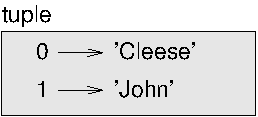
\includegraphics[scale=0.8]{figs/tuple1.pdf}}
%\caption{State diagram.}
\caption{แผนภาพสถานะ.}
\label{fig.tuple1}
\end{figure}

%But in a larger diagram you might want to leave out the
%details.  For example, a diagram of the telephone directory might
%appear as in Figure~\ref{fig.dict2}.
%
แต่ในแผนภาพที่ใหญ่ขึ้น เราไม่ต้องลงรายละเอียดขนาดนั้น.
ตัวอย่างเช่น แผนภาพของสมุดโทรศัพท์ อาจจะเป็นดังแสดงในรูป~\ref{fig.dict2}.
%
%Here the tuples are shown using Python syntax as a graphical
%shorthand.  
%The telephone number in the diagram is the complaints line
%for the BBC, so please don't call it.
%
ทูเพิลในแผนภาพ แสดงง่าย ๆ ด้วยไวยกรณ์ของไพธอน.

\begin{figure}
\centerline
{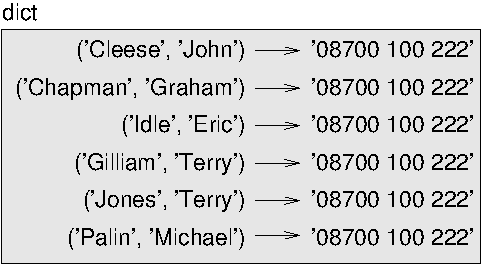
\includegraphics[scale=0.8]{figs/dict2.pdf}}
%\caption{State diagram.}
\caption{แผนภาพสถานะ.}
\label{fig.dict2}
\end{figure}



%\section{Sequences of sequences}
\section{ลำดับข้อมูลของลำดับข้อมูล}
\index{sequence}
\index{ลำดับข้อมูล}

%I have focused on lists of tuples, but almost all of the examples in
%this chapter also work with lists of lists, tuples of tuples, and
%tuples of lists.  To avoid enumerating the possible combinations, it
%is sometimes easier to talk about sequences of sequences.
%

เราได้ดูกันเรื่อง ลิสต์ของทูเพิล
แต่เกือบทั้งหมดของตัวอย่างในบทนี้ สามารถใช้กับ ลิสต์ของลิสต์
ทูเพิลของทูเพิล และทูเพิลของลิสต์ได้.
เพื่อไม่ต้องสาธยาย ทุก ๆ คู่ พวกนี้. %ของลำดับข้อมูลของลำดับข้อมูล
ว่าไปแล้ว บางครั้ง มันก็ง่ายกว่า ที่จะอ้างถึงคู่เหล่านี้เป็น ลำดับข้อมูลของลำดับข้อมูล.


%In many contexts, the different kinds of sequences (strings, lists and
%tuples) can be used interchangeably.  So how should you choose one
%over the others?

ในหลาย ๆ บริบท ลำดับข้อมูลหลาย ๆ ชนิด (สายอักขระ ลิสต์ และทูเพิล)
สามารถที่จะเลือกใช้อันไหนก็ได้.
แล้วเราจะเลือกอย่างไร ว่าชนิดไหนดีกว่าชนิดอื่น ๆ
%
\index{string}
\index{list}
\index{tuple}
\index{mutability}
\index{immutability}
\index{สายอักขระ}
\index{ลิสต์}
\index{ทูเพิล}
\index{การสามารถเปลี่ยนแปลงได้}
\index{การไม่สามารถเปลี่ยนแปลงได้}


%To start with the obvious, strings are more limited than other
%sequences because the elements have to be characters.  They are
%also immutable.  If you need the ability to change the characters
%in a string (as opposed to creating a new string), you might
%want to use a list of characters instead.

เริ่มจากเรื่องชัด ๆ ก่อน
สายอักขระจะค่อนข้างจำกัดกว่าลำดับข้อมูลชนิดอื่น ๆ
เพราะว่า อิลิเมนต์ของมัน ต้องเป็นอักขระเท่านั้น.
นอกจากนั้น สายอักขระ ยังเป็นลำดับข้อมูลชนิดที่ไม่สามารถเปลี่ยนแปลงได้.
ถ้าเราต้องการลำดับข้อมูลที่สามารถเปลี่ยนอักขระในลำดับได้ 
(ซึ่งต่างจาก การสร้างสายอักขระใหม่)
เราอาจจะเลือกใช้ลิสต์ของอักขระแทน.


%Lists are more common than tuples, mostly because they are mutable.
%But there are a few cases where you might prefer tuples:

เราจะเห็น การใช้ลิสต์บ่อยกว่าการใช้ทูเพิล
ส่วนใหญ่เพราะว่า ลิสต์ เป็นลำดับข้อมูลชนิดสามารถเปลี่ยนแปลงได้.
แต่ก็จะมีบางกรณี ที่อาจจะเหมาะกับทูเพิลมากกว่า

\begin{enumerate}

%\item In some contexts, like a {\tt return} statement, it is
%syntactically simpler to create a tuple than a list.

\item ในบางบริบท เช่น คำสั่ง \texttt{return} 
มันสะดวกที่จะสร้างทูเพิล มากกว่าสร้างลิสต์
(ไวยากรณ์ของทูเพิลสะดวกกว่า 
เช่น \texttt{return a,b} เปรียบเทียบกับ \texttt{return [a,b]})

%\item If you want to use a sequence as a dictionary key, you
%have to use an immutable type like a tuple or string.

\item เราต้องการลำดับข้อมูลเป็นกุญแจของดิกชันนารี
เราต้องใช้ลำดับข้อมูลชนิดที่ไม่สามารถเปลี่ยนแปลงได้ เช่น ทูเพิล หรือ สายอักขระ.

%\item If you are passing a sequence as an argument to a function,
%using tuples reduces the potential for unexpected behavior
%due to aliasing.

\item ถ้าเราต้องการส่งค่าของลำดับข้อมูล เป็นอาร์กิวเมนต์ให้กับฟังก์ชัน
การใช้ทูเพิล จะช่วยลดความเสี่ยงของพฤติกรรมจากการทำสมนาม.

\end{enumerate}

%Because tuples are immutable, they don't provide methods like {\tt %  sort} and {\tt reverse}, which modify existing lists.  But Python
%provides the built-in function {\tt sorted}, which takes any sequence
%and returns a new list with the same elements in sorted order, and
%{\tt reversed}, which takes a sequence and returns an iterator that
%traverses the list in reverse order.

เพราะว่า ทูเพิลเป็นลำดับข้อมูลชนิดที่ไม่สามารถเปลี่ยนแปลงได้
ทูเพิลจึงไม่มีพวกเมธอด เช่น \texttt{sort} และ \texttt{reverse}
ซึ่งไปแก้ไขค่าของลิสต์.
แต่ไพธอนก็ยังมีฟังก์ชันสำเร็จรูป \texttt{sorted} 
ที่รับลำดับข้อมูล แล้วรีเทิร์นลิสต์ของอิลิเมนต์นั้น ๆ ที่เรียงลำดับแล้วออกมาให้
และฟังก์ชันสำเร็จรูป \texttt{reversed} ที่รับลำดับข้อมูล แล้วรีเทิร์นตัววนซ้ำที่ใช้ท่องลิสต์ในลำดับถอยหลังออกมาให้.
%
\index{sorted function}
\index{function!sorted} \index{reversed function}
\index{function!reversed}
\index{iterator}
\index{ฟังก์ชัน!sorted}
\index{ฟังก์ชัน!reversed}
\index{ตัววนซ้ำ}

%\section{Debugging}
\section{การดีบัก}
\index{debugging}
\index{data structure}
\index{shape error}
\index{error!shape}
\index{การดีบัก}
\index{โครงสร้างข้อมูล}
\index{ข้อผิดพลาด!shape}

%Lists, dictionaries and tuples are examples of {\bf data
%  structures}; in this chapter we are starting to see compound data
%structures, like lists of tuples, or dictionaries that contain tuples
%as keys and lists as values.  Compound data structures are useful, but
%they are prone to what I call {\bf shape errors}; that is, errors
%caused when a data structure has the wrong type, size, or structure.
%For example, if you are expecting a list with one integer and I
%give you a plain old integer (not in a list), it won't work.

ลิสต์ ดิกชันนารี และทูเพิล เป็นตัวอย่างของ \textbf{โครงสร้างข้อมูล} (\textbf{data structures})
ในบทนี้ เราได้เริ่มเห็น\textit{โครงสร้างข้อมูลประกอบ} (\textit{compound data structure})
เช่น ลิสต์ของทูเพิล หรือ ดิกชันนารีที่ใช้ทูเพิลเป็นกุญแจ และลิสต์เป็นค่า.
โครงสร้างข้อมูลประกอบ มีประโยชน์มาก
แต่ก็เป็นความเสี่ยงให้เกิดข้อผิดพลาด แบบที่อาจจะเรียกว่า \textbf{ข้อผิดพลาดจากสัดส่วน} (\textbf{shape error}).
นั่นคือ ข้อผิดพลาด ที่เกิดเมื่อใช้โครงสร้างข้อมูลผิดชนิด ผิดขนาด หรือผิดโครงสร้าง.
ตัวอย่าง 
ถ้าโปรแกรมหรือฟังก์ชันรอรับลิสต์ที่มีเลขจำนวนเต็มหนึ่งตัว 
แต่เราให้เลขจำนวนเต็มหนึ่งตัว (เลขจำนวนเต็มแบบดั่งเดิม ไม่ใช่อยู่ในลิสต์)
มันจะไม่ทำงาน.
%
\index{structshape module}
\index{module!structshape}
\index{โมดูล!structshape}


%To help debug these kinds of errors, I have written a module
%called {\tt structshape} that provides a function, also called
%{\tt structshape}, that takes any kind of data structure as
%an argument and returns a string that summarizes its shape.
%You can download it from \url{http://thinkpython2.com/code/structshape.py}

เพื่อจะช่วยดีบักข้อผิดพลาดจากสัดส่วนพวกนี้
%ผู้เขียน (อัลเลน ดาวนี่)
หนังสือเล่มได้เตรียมโมดูลพิเศษไว้ให้ ชื่อว่า \texttt{structshape} 
ที่มีฟังก์ชัน \texttt{structshape}
ที่รับโครงสร้างข้อมูลใด ๆ เป็นอาร์กิวเมนต์ แล้วรีเทิร์นสายอักขระที่สรุปสัดส่วนของข้อมูลออกมา.
โมดูลนี้สามารถดาวน์โหลดได้จาก
\url{http://thinkpython2.com/code/structshape.py}

%Here's the result for a simple list:
ตัวอย่างผลลัพธ์สำหรับลิสต์ง่าย ๆ

\begin{verbatim}
>>> from structshape import structshape
>>> t = [1, 2, 3]
>>> structshape(t)
'list of 3 int'
\end{verbatim}
%
%A fancier program might write ``list of 3 int{\em s}'', but it
%was easier not to deal with plurals.  
%
โปรแกรมที่หรูหราซับซ้อนขึ้น อาจจะสามารถรายงาน
``list of 3 int\textbf{s}'' ออกมาได้
แต่ว่ามันง่ายกว่า ที่จะไม่ต้องไปยุ่งกับรูปพหูพจน์ของภาษาอังกฤษ.


%Here's a list of lists:
อันนี้เป็นตัวอย่าง เมื่อใช้กับลิสต์ของลิสต์

\begin{verbatim}
>>> t2 = [[1,2], [3,4], [5,6]]
>>> structshape(t2)
'list of 3 list of 2 int'
\end{verbatim}
%
%If the elements of the list are not the same type,
%{\tt structshape} groups them, in order, by type:
%
ถ้าอิลิเมนต์ของลิสต์ไม่ใช่ชนิดเดียวกัน
\texttt{structshape} จับมันรวมกลุ่มกัน ตามลำดับชนิด ดังเช่น

\begin{verbatim}
>>> t3 = [1, 2, 3, 4.0, '5', '6', [7], [8], 9]
>>> structshape(t3)
'list of (3 int, float, 2 str, 2 list of int, int)'
\end{verbatim}
%
%Here's a list of tuples:
%
อันนี้ตัวอย่าง ลิสต์ของทูเพิล

\begin{verbatim}
>>> s = 'abc'
>>> lt = list(zip(t, s))
>>> structshape(lt)
'list of 3 tuple of (int, str)'
\end{verbatim}
%
%And here's a dictionary with 3 items that map integers to strings.
%
และอันนี้ตัวอย่าง ดิกชันนารีที่มี 3 รายการที่แปลงเลขจำนวนเต็มไปเป็นสายอักขระ.

\begin{verbatim}
>>> d = dict(lt) 
>>> structshape(d)
'dict of 3 int->str'
\end{verbatim}
%
%If you are having trouble keeping track of your data structures,
%{\tt structshape} can help.
%
ถ้าเรามีปัญหาการตรวจสอบโครงสร้างข้อมูล
\texttt{structshape} อาจจะช่วยได้.

%\section{Glossary}
\section{อภิธานศัพท์}

\begin{description}

\item[ทูเพิล (tuple):] 
%An immutable sequence of elements.
ลำดับของอิลิเมนต์ที่ไม่สามารถเปลี่ยนแปลงค่าได้
\index{tuple}
\index{ทูเพิล}

\item[การกำหนดค่าทูเพิล (tuple assignment):] 
%An assignment with a sequence on the
%right side and a tuple of variables on the left.  The right
%side is evaluated and then its elements are assigned to the
%variables on the left.
การกำหนดค่าที่มีข้อมูลลำดับอยู่ทางขวามือ
และมีทูเพิลของตัวแปรต่าง ๆ อยู่ซ้ายมือ.
ค่าต่าง ๆ ทางขวามือจะถูกประมวลผลก่อน แล้วจึงกำหนดค่าให้กับตัวแปรต่าง ๆ ทางซ้ายมือ.
%
\index{tuple assignment}
\index{assignment!tuple}
\index{การกำหนดค่าทูเพิล}

\item[การรวบรวม (gather):] 
%The operation of assembling a variable-length
%argument tuple.
การดำเนินการประกอบตัวแปรทูเพิลขึ้นจากตัวแปรอาร์กิวเมนต์หลาย ๆ ตัว (อาร์กิวเมนต์ความยาวแปรผัน)
\index{gather}
\index{การรวบรวม}

\item[การแยกกระจาย (scatter):] 
%The operation of treating a sequence as a list of
%arguments.
การดำเนินการแยกกระจายค่ารายการต่าง ๆ ในตัวแปรลำดับข้อมูล
ไปให้กับอาร์กิวเมนต์ต่าง ๆ แต่ละตัว
\index{scatter}
\index{การกระจาย}

\item[ซิปออปเจ๊คต์ (zip object):] 
%The result of calling a built-in function {\tt zip};
%an object that iterates through a sequence of tuples.
ผลลัพธ์จากการเรียกใช้ฟังก์ชันสำเร็จ \texttt{zip}
ซึ่งเป็นออปเจ็คต์ที่สามารถใช้ท่องสำรวจลำดับข้อมูลที่ได้
จากการประกอบสองลำดับข้อมูลเข้าด้วยกัน
\index{zip object}
\index{object!zip}
\index{ซิปออปเจ๊คต์}

\item[ตัววนซ้ำ (iterator):] 
%An object that can iterate through a sequence, but
%which does not provide list operators and methods.
ออปเจ๊คต์ที่สามารถวนสำรวจลำดับของข้อมูลได้
แต่ไม่ใช่ลิสต์ และไม่สามารถใช้ตัวดำเนินการหรือเมธอดของลิสต์ได้
\index{iterator}
\index{ตัววนซ้ำ}

\item[โครงสร้างข้อมูล (data structure):] 
%A collection of related values, often
%organized in lists, dictionaries, tuples, etc.
การรวบรวมค่าข้อมูลต่าง ๆ ที่เกี่ยวข้องกัน
มักถูกจัดการเป็น ลิสต์ ดิกชันนารี หรือ ทูเพิล เป็นต้น
\index{data structure}
\index{โครงสร้างข้อมูล}

\item[ข้อผิดพลาดจากสัดส่วน (shape error):] 
%An error caused because a value has the
%wrong shape; that is, the wrong type or size.
ข้อผิดพลาดจากค่าข้อมูลที่ได้ผิดสัดส่วนที่คาดหวัง
นั่นคือ อาจจะผิดชนิดหรือขนาด
\index{shape}

\end{description}

\section{แบบฝึกหัด}
%\section{Exercises}

\begin{exercise}

%Write a function called \verb"most_frequent" that takes a string and
%prints the letters in decreasing order of frequency.  Find text
%samples from several different languages and see how letter frequency
%varies between languages.  Compare your results with the tables at
%\url{http://en.wikipedia.org/wiki/Letter_frequencies}.  Solution:
%\url{http://thinkpython2.com/code/most_frequent.py}.  \index{letter
%  frequency} \index{frequency!letter}

เขียนฟังก์ชันชื่อ \verb|most_frequent| ที่รับสายอักขระ
และพิมพ์ตัวอักษรออกมา โดยเรียงลำดับตามความถี่จากน้อยไปมาก.
ลองหาข้อความตัวอย่างจากหลาย ๆ ภาษา 
และดูว่าความถี่ของแต่ละอักษรแตกต่างอย่างไรบ้างสำหรับแต่ละภาษา.
ลองเปรียบเทียบผลลัพธ์ที่ได้กับตารางใน
\url{http://en.wikipedia.org/wiki/Letter_frequencies}.  
โปรแกรมเฉลย:
\url{http://thinkpython2.com/code/most_frequent.py}.  \index{letter frequency} 
\index{frequency!letter}
\index{ความถี่ตัวอักษร}
\index{ความถี่!ตัวอักษร}


\end{exercise}
\vspace{0.5cm}


\begin{exercise}
\label{anagrams}
\index{anagram set}
\index{set!anagram}
\index{คำสลับอักษร}

%More anagrams!
\textit{คำสลับอักษร}อีก!

\begin{enumerate}

%\item Write a program
%that reads a word list from a file (see Section~\ref{wordlist}) and
%prints all the sets of words that are anagrams.

\item เขียนโปรแกรม ให้อ่านรายการคำ จากไฟล์ (ดูหัวข้อ~\ref{wordlist})
และพิมพ์กลุ่มคำทั้งหมดที่เป็น\textit{คำสลับอักษร} (\textit{anagram}).

%Here is an example of what the output might look like:

ข้างล่างเป็นตัวอย่างของเอาต์พุต

\begin{verbatim}
['deltas', 'desalt', 'lasted', 'salted', 'slated', 'staled']
['retainers', 'ternaries']
['generating', 'greatening']
['resmelts', 'smelters', 'termless']
\end{verbatim}
%
%Hint: you might want to build a dictionary that maps from a
%collection of letters to a list of words that can be spelled with those
%letters.  The question is, how can you represent the collection of
%letters in a way that can be used as a key?
%
คำใบ้: เราอาจจะต้องสร้างดิกชันนารี
ที่แปลงจากกลุ่มหมู่ของตัวอักษร
ไปเป็นลิสต์ของคำ ที่สามารถสะกดด้วยอักษรเหล่านั้น.
คำถามคือ เราจะใช้กลุ่มหมู่ของตัวอักษรไปเป็นกุญแจของดิกชันนารีได้อย่างไร

%\item Modify the previous program so that it prints the longest list
%of anagrams first, followed by the second longest, and so on.
%\index{Scrabble}
%\index{bingo}

\item ดัดแปลงโปรแกรมข้างต้น ให้พิมพ์ลิสต์ที่ยาวที่สุดก่อน (ลิสต์ที่มีจำนวนคำสลับอักษรมากที่สุด) ตามด้วยลิสต์ที่ยาวอันดับสอง ไปเรื่อย ๆ
\index{Scrabble}
\index{bingo}

%\item In Scrabble a ``bingo'' is when you play all seven tiles in
%your rack, along with a letter on the board, to form an eight-letter
%word.  What collection of 8 letters forms the most possible bingos?
%Hint: there are seven.

\item ในเกมสแคร์บเบิล (Scrabble) 
เราจะได้``บิงโก'' เมื่อเราลงตัวทั้งเจ็ดตัวของเราได้ และพอมันไปรวมกับตัวที่วางในบอร์ดแล้ว ได้เป็นคำแปดตัวอักษร.
คำแปดตัวอักษรใดบ้างที่น่าจะได้บิงโกมากที่สุด?
คำใบ้: มีเจ็ดคำ.

% (7, ['angriest', 'astringe', 'ganister', 'gantries', 'granites',
% 'ingrates', 'rangiest'])

%Solution: \url{http://thinkpython2.com/code/anagram_sets.py}.

เฉลย: \url{http://thinkpython2.com/code/anagram_sets.py}.


\end{enumerate}
\end{exercise}
\vspace{0.5cm}


\begin{exercise}
\index{metathesis}
\index{คำสลับเสียง}

%Two words form a ``metathesis pair'' if you can transform one into the
%other by swapping two letters; for example, ``converse'' and
%``conserve''.  Write a program that finds all of the metathesis pairs
%in the dictionary.  Hint: don't test all pairs of words, and don't
%test all possible swaps.  Solution:
%\url{http://thinkpython2.com/code/metathesis.py}.  Credit: This
%exercise is inspired by an example at \url{http://puzzlers.org}.

คำสองคำจะเรียกว่าเป็น ``คู่สลับเสียง'' (metathesis pair)
ถ้าเราสามารถแปลงคำหนึ่งเป็นอีกคำได้โดยการสลับสองตัวอักษร
เช่น ``converse'' และ ``conserve''.
เขียนโปรแกรมที่หาคู่สลับเสียงทั้งหมดออกมาจากพจนานุกรม.
คำใบ้: อย่าทดสอบทุก ๆ คู่ของคำ
และอย่าทดสอบทุก ๆ การสลับอักษร.
เฉลย: \url{http://thinkpython2.com/code/metathesis.py}.  
%
ขอบคุณ: 
แบบฝึกหัดนี้ได้รับแรงบันดาลใจจากตัวอย่างใน \url{http://puzzlers.org}.

\end{exercise}
\vspace{0.5cm}


\begin{exercise}
\index{Car Talk}
\index{Puzzler}

%Here's another Car Talk Puzzler
%(\url{http://www.cartalk.com/content/puzzlers}):

อีกปริศนาจากจอมปริศนาคาร์ทอร์ค
(\url{http://www.cartalk.com/content/puzzlers}):

\begin{quote}
%What is the longest English word, that remains a valid English word,
%as you remove its letters one at a time?

คำไหนในภาษาอังกฤษที่ยาวที่สุด ที่ถ้าดึงตัวอักษรออกทีละตัว แล้วส่วนที่เหลือยังเป็นคำในภาษาอังกฤษอยู่

%Now, letters can be removed from either end, or the middle, but you
%can't rearrange any of the letters. Every time you drop a letter, you
%wind up with another English word. If you do that, you're eventually
%going to wind up with one letter and that too is going to be an
%English word---one that's found in the dictionary. I want to know
%what's the longest word and how many letters does it
%have?

ตัวอักษรที่เอาออกอาจจะเป็นตัวที่ต้น หรือปลาย หรือกลางคำก็ได้
แต่ต้องไม่มีการเรียงตัวอักษรที่เหลือใหม่.
ทุก ๆ ครั้งที่เอาตัวอักษรออก ส่วนที่เหลือต้องเป็นคำภาษาอังกฤษ.
ทำไปเรื่อย ๆ สุดท้ายเราก็จะเหลือแต่ตัวอักษรตัวเดียว และตัวอักษรตัวสุดท้ายที่เหลืออยู่ก็ต้องเป็นคำในภาษาอังกฤษด้วย (มีอยู่ในพจนานุกกรม).
ผมอยากจะรู้ว่า คำแบบนี้ที่ยาวที่สุดคือคำว่าอะไร และมันยาวเท่าไร?

%I'm going to give you a little modest example: Sprite. Ok? You start
%off with sprite, you take a letter off, one from the interior of the
%word, take the r away, and we're left with the word spite, then we
%take the e off the end, we're left with spit, we take the s off, we're
%left with pit, it, and I.

ผมยกตัวอย่างเล็ก ๆ ให้อันหนึ่ง คำว่า sprite.
ถ้าเราเริ่มด้วย sprite เราเอาตัวอักษรหนึ่งออก เอาตัว r ออกจากกลางคำ
เราจะเหลือ spite.
จากนั้นเอา e ออกจากท้าย เราเหลือ spit.
เอา s ออก เราเหลือ pit แล้ว it แล้ว I.
 

\end{quote}
\index{reducible word}
\index{word, reducible}

เขียนโปรแกรมที่หาคำทั้งหมดที่สามารถลดรูปได้แบบนี้ แล้วหาคำที่ยาวที่สุด.
%Write a program to find all words that can be reduced in this way,
%and then find the longest one.

%This exercise is a little more challenging than most, so here are
%some suggestions:

แบบฝึกหัดนี้ค่อนข้างจะยากกว่าอันอื่น ๆ
คำแนะนำคือ
\begin{enumerate}

%\item You might want to write a function that takes a word and
%  computes a list of all the words that can be formed by removing one
%  letter.  These are the ``children'' of the word.  
%\index{recursive definition}
%\index{definition!recursive}

\item เราอาจจะเขียนฟังก์ชันที่รับอาร์กิวเมนต์เป็นคำในภาษาอังกฤษ
แล้วหาลิสต์ของคำทั้งหมด ที่เกิดจากการตัดอักษรออกตัวหนึ่ง.
ลิสต์ของคำนี้เป็น ``ลูก'' ของคำ.
\index{recursive definition}
\index{definition!recursive}
\index{การเรียกซ้ำ}

%\item Recursively, a word is reducible if any of its children
%are reducible.  As a base case, you can consider the empty
%string reducible.

\item ทำแบบ\textit{การเรียกซ้ำ} คำจะลดรูปได้ ถ้าลูกของมันลดรูปได้.
และ\textit{กรณีฐาน} เราอาจจะนับสายอักขระว่างว่าสามารถลดรูปได้.

%\item The wordlist I provided, {\tt words.txt}, doesn't
%contain single letter words.  So you might want to add
%``I'', ``a'', and the empty string.

\item รายการคำที่ให้ \texttt{words.txt} ไม่มีคำอักษรเดี่ยว.
ดังนั้นเราอาจต้องเพิ่ม ``I'' และ ``a'' และสายอักขระว่าง ๆ เข้าไป.

\item To improve the performance of your program, you might want
to memoize the words that are known to be reducible.

\item เพื่อเพิ่มประสิทธิภาพของโปรแกรม เราอาจต้องจำคำต่าง ๆ ที่รู้แล้วว่าลดรูปได้ไว้.

\end{enumerate}

%Solution: \url{http://thinkpython2.com/code/reducible.py}.
เฉลย: \url{http://thinkpython2.com/code/reducible.py}.


\end{exercise}
\vspace{0.5cm}




%\begin{exercise}
%\url{http://en.wikipedia.org/wiki/Word_Ladder}
%\end{exercise}




\chapter{กรณีศึกษา การเลือกโครงสร้างข้อมูล}

%At this point you have learned about Python's core data structures,
%and you have seen some of the algorithms that use them.
%If you would like to know more about algorithms, this might be a good
%time to read Chapter~\ref{algorithms}.
%But you don't have to read it before you go on; you can read
%it whenever you are interested.

ถึงตอนนี้ เราได้เรียนโครงสร้างข้อมูลหลัก ๆ ของไพธอนไปแล้ว
และเราก็ได้เห็นอัลกอริทึมที่ใช้มันไปบ้างแล้วด้วย.
ถ้าอยากรู้เรื่องอัลกอริทึมมากขึ้น อาจถึงเวลาแล้วที่จะไปอ่านบท~\ref{algorithms}.
แต่ก็ไม่ได้จำเป็นว่าจะต้องอ่านบท~\ref{algorithms} ก่อนจะเรียนบทนี้ 
จริง ๆ จะอ่านบท~\ref{algorithms} ตอนไหนก็ได้ที่สนใจ.

%This chapter presents a case study with exercises that let
%you think about choosing data structures and practice using them.

บทนี้นำเสนอกรณีตัวอย่างด้วยแบบฝึกหัด 
ที่จะช่วยให้คิดเรื่องเลือกโครงสร้างข้อมูล และก็จะได้ฝึกใช้มันด้วย.

%\section{Word frequency analysis}
\section{การวิเคราะห์ความถี่คำ}
\label{analysis}

%As usual, you should at least attempt the exercises
%before you read my solutions.

เหมือนเคย ที่อย่างน้อย เราควรจะลองทำแบบฝึกหัดด้วยตัวเองก่อนที่จะไปเปิดดูเฉลย.

\begin{exercise}

%Write a program that reads a file, breaks each line into
%words, strips whitespace and punctuation from the words, and
%converts them to lowercase.

เขียนโปรแกรมให้อ่านไฟล์ แล้วแยกแต่ละบรรทัดออกเป็นคำ ๆ 
เอา\textit{ช่องว่างต่าง ๆ} (\textit{whitespace}) และ\textit{เครื่องหมายวรรคตอน}ต่าง ๆ (\textit{punctuation}) ออกจากคำ
และแปลงให้เป็น\textit{อักษรตัวเล็ก} (\textit{lowercase}).
\index{string module}
\index{module!string}
\index{โมดูล!สายอักขระ}


%Hint: The {\tt string} module provides a string named {\tt whitespace},
%which contains space, tab, newline, etc., and {\tt %  punctuation} which contains the punctuation characters.  Let's see
%if we can make Python swear:

คำใบ้: โมดูล \texttt{string} มีสายอักขระชื่อ \texttt{whitespace}
และสายอักขระชื่อ \texttt{punctuation}.
สายอักขระ \texttt{whitespace} มีอักขระช่องว่าง (space) อักขระตั้งระยะ (tab) อักขระขึ้นบรรทัดใหม่ (newline) เป็นต้น.
สายอักขระ \texttt{punctuation}  มีอักขระเครื่องหมายวรรคตอนต่าง ๆ.
ลองดู %กันว่า เราจะทำให้ไพธอนบ่นออกได้

\begin{verbatim}
>>> import string
>>> string.punctuation
'!"#$%&'()*+,-./:;<=>?@[\]^_`{|}~'
\end{verbatim}
%
%Also, you might consider using the string methods {\tt strip},
%{\tt replace} and {\tt translate}.
%
นอกจากนั้น อาจจะลองดูเมธอดของสายอักขระ เช่น เมธอด \texttt{strip} เมธอด \texttt{replace} และเมธอด \texttt{translate}.
%
\index{strip method}
\index{method!strip}
\index{replace method}
\index{method!replace}
\index{translate method}
\index{method!translate}
\index{เมธอด!strip}
\index{เมธอด!replace}
\index{เมธอด!translate}
\\
\end{exercise}


\begin{exercise}
\index{Project Gutenberg}

%Go to Project Gutenberg (\url{http://gutenberg.org}) and download 
%your favorite out-of-copyright book in plain text format.

ลองดูโครงการกูเทินแบร์ค (\url{http://gutenberg.org})
และดาวน์โหลดหนังสือที่ชอบ ที่หมดลิขสิทธิ์ไปแล้ว.
ดาวน์โหลดไฟล์มาในรูป\textit{ข้อความธรรมดา} (\textit{plain text}).
\index{plain text}
\index{text!plain}
%
%Modify your program from the previous exercise to read the book
%you downloaded, skip over the header information at the beginning
%of the file, and process the rest of the words as before.
%
ดัดแปลงโปรแกรมจากแบบฝึกหัดที่แล้ว เพื่ออ่านหนังสือที่ดาวน์โหลดมา
ข้ามพวกข้อมูลประกอบที่อยู่ตอนต้นของไฟล์
และประมวลผลส่วนที่เหลือ.
%
%Then modify the program to count the total number of words in
%the book, and the number of times each word is used.

จากนั้น ดัดแปลงโปรแกรมให้นับจำนวนคำทั้งหมดในหนังสือ
และจำนวนครั้งที่แต่ละคำปรากฏ.
\index{word frequency}
\index{frequency!word}
\index{ความถี่คำ}
%
%Print the number of different words used in the book.  Compare
%different books by different authors, written in different eras.
%Which author uses the most extensive vocabulary?

พิมพ์จำนวนคำต่าง ๆ ที่พบในหนังสือ.
เปรียบเทียบหนังสือจากนักเขียนต่าง ๆ ที่เขียนคนละยุค.
นักเขียนคนไหนที่ใช้คำศัพท์ได้กว้างขวางหลากหลายที่สุด?
\\
\end{exercise}


\begin{exercise}

%Modify the program from the previous exercise to print the
%20 most frequently used words in the book.
%
ดัดแปลงโปรแกรมจากแบบฝึกหัดที่แล้ว
เพื่อพิมพ์คำที่ใช้มากที่สุด 20 คำในหนังสือ.
\\
\end{exercise}


\begin{exercise}

%Modify the previous program to read a word list (see
%Section~\ref{wordlist}) and then print all the words in the book that
%are not in the word list.  How many of them are typos?  How many of
%them are common words that {\em should} be in the word list, and how
%many of them are really obscure?
%
ดัดแปลงโปรแกรมที่แล้ว เพื่อให้อ่านลิสต์ของคำ (ดูหัวข้อ~\ref{wordlist})
แล้วพิมพ์ทุกคำในหนังสือที่ไม่ได้อยู่ในลิสต์ของคำ.
มีกี่คำที่เจอที่พิมพ์ผิด?
มีกี่คำที่เป็นคำทั่ว ๆ ไป ที่\textbf{ควร}จะอยู่ในลิสต์ของคำ 
และมีกี่คำที่คลุมเครือ?
\\
\end{exercise}


%\section{Random numbers}
\section{ตัวเลขค่าสุ่ม}
\index{random number}
\index{number, random}
\index{deterministic}
\index{pseudorandom}
\index{ตัวเลขค่าสุ่ม}


%Given the same inputs, most computer programs generate the same
%outputs every time, so they are said to be {\bf deterministic}.
%Determinism is usually a good thing, since we expect the same
%calculation to yield the same result.  For some applications, though,
%we want the computer to be unpredictable.  Games are an obvious
%example, but there are more.

ถ้าได้อินพุตเหมือน ๆ กัน
คอมพิวเตอร์(ส่วนใหญ่)จะให้เอาต์พุตออกมาเหมือนกันทุกครั้ง
ลักษณะแบบนี้ เรียกว่า \textbf{ลักษณะชี้เฉพาะ} (\textbf{deterministic}).
\index{ลักษณะชี้เฉพาะ}
\index{deterministic}
\textit{ลักษณะการชี้เฉพาะ}โดยทั่วไปแล้วมันก็ดี
เพราะว่า เรามั่นใจได้ว่า การคำนวณแบบเดียวกัน จะได้ผลออกมาแบบเดียวกัน.
แต่สำหรับงานบางลักษณะ
เราต้องการให้คอมพิวเตอร์มีลักษณะที่เดาไม่ได้บ้าง
เกมส์ก็เป็นตัวอย่างหนึ่ง แต่ยังมีตัวอย่างอื่น ๆ อีกมาก ที่ต้องลักษณะเดาไม่ได้.

%Making a program truly nondeterministic turns out to be difficult,
%but there are ways to make it at least seem nondeterministic.  One of
%them is to use algorithms that generate {\bf pseudorandom} numbers.
%Pseudorandom numbers are not truly random because they are generated
%by a deterministic computation, but just by looking at the numbers it
%is all but impossible to distinguish them from random.
%\index{random module}
%\index{module!random}

การที่จะเขียนโปรแกรมให้ไม่เป็น\textit{ลักษณะชี้เฉพาะ}เลย คือเดาไม่ได้จริง ๆ ทำยากมาก.
แต่ก็มีหลายวิธีที่ อย่างน้อย ก็ช่วยให้โปรแกรมดูเหมือนว่า ไม่เป็น\textit{ลักษณะชี้เฉพาะ}.
หนึ่งให้วิธีเหล่านั้นก็คือ ใช้อัลกอริทึมที่สร้างตัวเลข\textbf{สุ่มเทียม} (\textbf{pseudorandom}).
ค่าของตัวเลขสุ่มเทียม ไม่ได้ถูกสุ่มขึ้นมาจริง ๆ
แต่มันจะสร้างมาจากการคำนวณ\textit{ลักษณะชี้เฉพาะ}
ที่ทำให้ ตัวเลขที่ได้ ถ้าดูเผิน ๆ มันจะดูเหมือนว่าถูกสุ่มมา.
\index{random module}
\index{module!random}
\index{โมดูลการสุ่ม}
\index{โมดูล!random}


%The {\tt random} module provides functions that generate
%pseudorandom numbers (which I will simply call ``random'' from
%here on).
%\index{random function}
%\index{function!random}

โมดูล \texttt{random} มีฟังก์ชันต่าง ๆ ที่สามารถสร้างตัวเลขสุ่มเทียมได้ 
(ซึ่งตั้งแต่นี้ไป เราจะแค่เรียกสั้น ๆ ว่า ``สุ่ม'')
\index{random function}
\index{function!random}
\index{ฟังก์ชัน!random}

%The function {\tt random} returns a random float
%between 0.0 and 1.0 (including 0.0 but not 1.0).  Each time you
%call {\tt random}, you get the next number in a long series.  To see a
%sample, run this loop:

ฟังก์ชัน \texttt{random} จะให้จำนวนจริงที่มีค่าสุ่มมาระหว่าง 0.0 ถึง 1.0 (รวม 0.0 แต่ไม่รวม 1.0).
ทุกครั้งที่เราเรียก \texttt{random}
เราจะได้เลขสุ่มใหม่ ซึ่งเป็นเลขถัดไป ในลำดับที่ยาวมาก.
เพื่อให้เห็นตัวอย่าง ลองรันลูปนี้:

\begin{verbatim}
import random

for i in range(10):
    x = random.random()
    print(x)
\end{verbatim}
%
%The function {\tt randint} takes parameters {\tt low} and
%{\tt high} and returns an integer between {\tt low} and
%{\tt high} (including both).
%\index{randint function}
%\index{function!randint}
%
ฟังก์ชัน \texttt{randint} รับพารามิเตอร์ \texttt{low} และ \texttt{high}
แล้วให้ค่าสุ่มเลขจำนวนเต็มระหว่าง \texttt{low} และ \texttt{high} ออกมา 
(รวมค่า \texttt{low} และ \texttt{high} ด้วย).
\index{randint function}
\index{function!randint}
\index{ฟังก์ชัน!randint}

\begin{verbatim}
>>> random.randint(5, 10)
5
>>> random.randint(5, 10)
9
\end{verbatim}
%
%To choose an element from a sequence at random, you can use
%{\tt choice}:
%\index{choice function}
%\index{function!choice}
%
เพื่อเลือกอิลิเมนต์จากลำดับแบบสุ่ม
เราสามารถใช้ \texttt{choice} ได้:
\index{choice function}
\index{function!choice}
\index{ฟังก์ชัน!choice}

\begin{verbatim}
>>> t = [1, 2, 3]
>>> random.choice(t)
2
>>> random.choice(t)
3
\end{verbatim}
%
%The {\tt random} module also provides functions to generate
%random values from continuous distributions including
%Gaussian, exponential, gamma, and a few more.
%
โมดูล \texttt{random} ยังมีฟังก์ชันต่าง ๆ
ที่สร้างค่าสุ่มจาก\textit{การแจกแจงต่อเนื่อง} (\textit{continuous distributions})
รวมถึง การแจกแจงแบบเกาส์เซียน (Gaussian distribution)
การแจกแจงแบบเลขชี้กำลัง (exponential distribution)
การแจกแจงแกมมา (gamma distribution)
เป็นต้น


\begin{exercise}
\index{histogram!random choice}

%Write a function named \verb"choose_from_hist" that takes
%a histogram as defined in Section~\ref{histogram} and returns a 
%random value from the histogram, chosen with probability
%in proportion to frequency.  For example, for this histogram:

เขียนฟังก์ชันชื่อ \verb|choose_from_hist|
ที่รับฮิสโตแกรม (histogram) แบบที่กำหนดในหัวข้อ~\ref{histogram}
และรีเทิร์นค่าสุ่มจากฮิสโตแกรม
นั่นคือ เลือกค่าสุ่มด้วยความน่าจะเป็น ให้เป็นสัดส่วนตามความถี่ในฮิสโตแกรม.
ตัวอย่าง สำหรับฮิสโตแกรมนี้:

\begin{verbatim}
>>> t = ['a', 'a', 'b']
>>> hist = histogram(t)
>>> hist
{'a': 2, 'b': 1}
\end{verbatim}
%
%your function should return \verb"'a'" with probability $2/3$ and \verb"'b'"
%with probability $1/3$.
%
ฟังก์ชันควรจะให้ \verb|a| ออกมาด้วยความน่าจะเป็น $2/3$ 
และให้ \verb|b| ออกมาด้วยความน่าจะเป็น $1/3$.
%
\end{exercise}


%\section{Word histogram}
\section{ฮิสโตแกรมคำ}

%You should attempt the previous exercises before you go on.
%You can download my solution from
% \url{http://thinkpython2.com/code/analyze_book1.py}.  You will
%also need \url{http://thinkpython2.com/code/emma.txt}.

ควรจะลองทำแบบฝึกหัดที่แล้ว ก่อนจะอ่านเรื่องนี้ต่อ.
โปรแกรมเฉลยดาวน์โหลดได้จาก
\url{http://thinkpython2.com/code/analyze_book1.py}.
และก็อาจจะต้องการ อันนี้ด้วย
\url{http://thinkpython2.com/code/emma.txt}.

%Here is a program that reads a file and builds a histogram of the
%words in the file:
%\index{histogram!word frequencies}

นี่เป็นโปรแกรม ที่อ่านไฟล์ และสร้างฮิสโตแกรมของคำต่าง ๆ ในไฟล์:
\index{histogram!word frequencies}
\index{ฮิสโตแกรม!word frequencies}

\begin{verbatim}
import string

def process_file(filename):
    hist = dict()
    fp = open(filename)
    for line in fp:
        process_line(line, hist)
    return hist

def process_line(line, hist):
    line = line.replace('-', ' ')
    
    for word in line.split():
        word = word.strip(string.punctuation + string.whitespace)
        word = word.lower()
        hist[word] = hist.get(word, 0) + 1

hist = process_file('emma.txt')
\end{verbatim}
%
%This program reads {\tt emma.txt}, which contains the text of {\em
%  Emma} by Jane Austen.
%\index{Austin, Jane}
%
โปรแกรมนี้อ่านไฟล์ {\tt emma.txt}
เป็นนิยายเรื่อง \textit{เอ็มม่า} (\textit{Emma}) เขียนโดน เจน ออสเทน (Jane Austen).
\index{Austin, Jane}

%\verb"process_file" loops through the lines of the file,
%passing them one at a time to \verb"process_line".  
%The histogram
%{\tt hist} is being used as an accumulator.
%\index{accumulator!histogram}
%\index{traversal}

ฟังก์ชัน \verb|process_file| ลูปวนทีละบรรทัดของไฟล์ 
ส่งแต่ละบรรทัดไปที่ \verb|process_line|.
ฮิสโตแกรม \texttt{hist} ถูกใช้เป็น \textit{ตัวสะสม} (\textit{accumulator}) สะสมค่าความถี่จากแต่ละบรรทัด.
\index{accumulator!histogram}
\index{traversal}

%\verb"process_line" uses the string method {\tt replace} to replace
%hyphens with spaces before using {\tt split} to break the line into a
%list of strings.  It traverses the list of words and uses {\tt strip}
%and {\tt lower} to remove punctuation and convert to lower case.  (It
%is a shorthand to say that strings are ``converted''; remember that
%strings are immutable, so methods like {\tt strip} and {\tt lower}
%return new strings.)

ฟังก์ชัน \verb|process_line| ใช้เมธอดของสายอักขระ \texttt{replace}
เพื่อแทนที่ เครื่องหมายยัติภังค์ (hyphen) ด้วยช่องว่าง
ก่อนที่จะใช้เมธอด \texttt{split} เพื่อแยกบรรทัด ออกไปเป็นลิสต์ของสายอักขระ.
มันท่องสำรวจลิสต์ของคำ และใช้เมธอด \texttt{strip} และเมธอด \texttt{lower}
เพื่อตัด\textit{เครื่องหมายวรรคตอน}ต่าง ๆ และแปลงเป็นอักษรตัวเล็ก.
(อาจจะพูดสั้น ๆ ว่า สายอักขระถูก``แปลง'' 
แต่ถ้าจำได้ สายอักขระเป็นข้อมูลที่\textit{ไม่สามารถเปลี่ยนแปลงได้}
ดังนั้น เมธอดพวก \texttt{strip} และ \texttt{lower} จะให้สายอักขระใหม่ออกมา.)

%Finally, \verb"process_line" updates the histogram by creating a new
%item or incrementing an existing one.
%\index{update!histogram}

สุดท้าย ฟังก์ชัน \verb|process_line| ปรับค่าของฮิสโตแกรม
โดยการสร้างรายการสำหรับคำใหม่ หรือเพิ่มค่าให้กับคำที่มีอยู่แล้ว.
\index{update!histogram}

%To count the total number of words in the file, we can add up
%the frequencies in the histogram:

เพื่อจะนับจำนวนคำทั้งหมดในไฟล์
เราสามารถรวมความถี่ต่าง ๆ ในฮิสโตแกรมได้:

\begin{verbatim}
def total_words(hist):
    return sum(hist.values())
\end{verbatim}
%
%The number of different words is just the number of items in
%the dictionary:
%
จำนวนคำศัพท์ ก็คือจำนวนรายการในดิกชันนารี:

\begin{verbatim}
def different_words(hist):
    return len(hist)
\end{verbatim}
%
%Here is some code to print the results:
%
นี่เป็นโปรแกรมสำหรับพิมพ์ผลลัพธ์ออกมา:

\begin{verbatim}
print('Total number of words:', total_words(hist))
print('Number of different words:', different_words(hist))
\end{verbatim}
%
%And the results:
%
และผลลัพธ์ที่ได้:

\begin{verbatim}
Total number of words: 161080
Number of different words: 7214
\end{verbatim}
%

%\section{Most common words}
\section{คำที่พบบ่อยที่สุด}

%To find the most common words, we can make a list of tuples,
%where each tuple contains a word and its frequency,
%and sort it.

เพื่อจะหาคำศัพท์ที่ใช้บ่อยที่สุด
เราสามารถสร้างลิสต์ของทูเพิล ที่แต่ละทูเพิลมีคำศัพท์และความถี่ของมัน
แล้วก็จัดเรียงมัน.

%The following function takes a histogram and returns a list of
%word-frequency tuples:

ฟังก์ชันต่อไปนี้รับฮิสโตแกรม และรีเทิร์นลิสต์ของทูเพิล ที่ทูเพิลเป็นคู่ของคำกับความถี่:

\begin{verbatim}
def most_common(hist):
    t = []
    for key, value in hist.items():
        t.append((value, key))

    t.sort(reverse=True)
    return t
\end{verbatim}

%In each tuple, the frequency appears first, so the resulting list is
%sorted by frequency.  Here is a loop that prints the ten most common
%words:

ในแต่ละทูเพิล ความถี่แสดงก่อนคำ 
และผลลัพธ์ก็เรียงลำดับตามความถี่จากมากไปน้อย.
นี่เป็นลูปที่พิมพ์คำสิบคำที่พบบ่อยที่สุดออกมา:

\begin{verbatim}
t = most_common(hist)
print('The most common words are:')
for freq, word in t[:10]:
    print(word, freq, sep='\t')
\end{verbatim}
%
%I use the keyword argument {\tt sep} to tell {\tt print} to use a tab
%character as a ``separator'', rather than a space, so the second
%column is lined up.  Here are the results from {\em Emma}:
%
อาร์กิวเมนต์ \texttt{sep} บอกคำสั่ง \texttt{print} ให้ใช้อักขระตั้งระยะ
เป็น ``ตัวแยก'' แทนช่องว่าง
ทำให้คอลัมน์ที่สองเรียงกันเป็นแนว.
นี่เป็นผลลัพธ์ที่ได้จากนิยาย\textit{เอ็มม่า}. 

\begin{verbatim}
The most common words are:
to      5242
the     5205
and     4897
of      4295
i       3191
a       3130
it      2529
her     2483
was     2400
she     2364
\end{verbatim}
%
%This code can be simplified using the {\tt key} parameter of
%the {\tt sort} function.  If you are curious, you can read about it
%at \url{https://wiki.python.org/moin/HowTo/Sorting}.
%
โปรแกรมนี้จริง ๆ สามารถเขียนให้ง่ายกว่านี้ได้ โดยใช้พารามิเตอร์ \texttt{key} ของฟังก์ชัน \texttt{sort}.
ถ้าสนใจ ลองศึกษาดูได้จาก \url{https://wiki.python.org/moin/HowTo/Sorting}.

%\section{Optional parameters}
\section{พารามิเตอร์เสริม}
\index{optional parameter}
\index{parameter!optional}

%We have seen built-in functions and methods that take optional
%arguments.  It is possible to write programmer-defined functions
%with optional arguments, too.  For example, here is a function that
%prints the most common words in a histogram
%\index{programmer-defined function}
%\index{function!programmer defined}

เราได้ดูฟังก์ชันสำเร็จรูป และเมธอดต่าง ๆ
ที่รับพารามิเตอร์เสริมมาแล้ว.
เราเองก็เขียนฟังก์ชันที่รับพารามิเตอร์เสริมได้เหมือนกัน.
ตัวอย่าง นี่เป็นฟังก์ชันที่พิมพ์คำที่พบบ่อยที่สุดในฮิสโตแกรมออกมา
\index{programmer-defined function}
\index{function!programmer defined}
\index{ฟังก์ชัน!เขียนขึ้นเอง}
\index{ฟังก์ชันเขียนขึ้นเอง}


\begin{verbatim}
def print_most_common(hist, num=10):
    t = most_common(hist)
    print('The most common words are:')
    for freq, word in t[:num]:
        print(word, freq, sep='\t')
\end{verbatim}

%The first parameter is required; the second is optional.
%The {\bf default value} of {\tt num} is 10.
%\index{default value}
%\index{value!default}

พารามิเตอร์แรกต้องใส่ 
แต่พารามิเตอร์ที่สองเป็นพารามิเตอร์เสริม 
ถ้าไม่ใส่ \texttt{num} จะใช้ค่า\textit{ดีฟอลท์} เป็น 10. 
\index{default value}
\index{value!default}
\index{ดีฟอลท์}

%If you only provide one argument:
ถ้าเรียกใช้ ด้วยหนึ่งอาร์กิวเมนต์:

\begin{verbatim}
print_most_common(hist)
\end{verbatim}

%{\tt num} gets the default value.  If you provide two arguments:
ตัวแปร \texttt{num} จะใช้ค่าดีฟอลท์.
แต่ถ้าเรียกใช้ ด้วยอาร์กิวเมนต์สองตัว:

\begin{verbatim}
print_most_common(hist, 20)
\end{verbatim}

%{\tt num} gets the value of the argument instead.  In other
%words, the optional argument {\bf overrides} the default value.
%\index{override}

ตัวแปร \texttt{num} จะใช้ค่าของอาร์กิวเมนต์.
พูดง่าย ๆ คือ อาร์กิวเมนต์เสริมไป\textbf{แทนที่}ค่าดีฟอลท์.

%If a function has both required and optional parameters, all
%the required parameters have to come first, followed by the
%optional ones.

ถ้าฟังก์ชันมีทั้งพารามิเตอร์บังคับ และพารามิเตอร์เสริม
พารามิเตอร์บังคับทุกตัวต้องมาก่อน แล้วค่อยตามด้วยพารามิเตอร์เสริม.

%\section{Dictionary subtraction}
\section{การลบดิกชันนารี}
\label{dictsub}
\index{dictionary!subtraction}
\index{subtraction!dictionary}

%Finding the words from the book that are not in the word list
%from {\tt words.txt} is a problem you might recognize as set
%subtraction; that is, we want to find all the words from one
%set (the words in the book) that are not in the other (the
%words in the list).

การหาคำที่มีในหนังสือ แต่ไม่มีในลิสต์ของคำศัพท์จาก \texttt{words.txt}
ก็เหมือนกับปัญหาการลบของเซต.
นั่นคือ เราต้องการหาคำทุกคำจากเซตหนึ่ง (คำต่าง ๆ ในหนังสือ) ที่ไม่ได้อยู่ในอีกเซตหนึ่ง (คำต่าง ๆ ในลิสต์).

%{\tt subtract} takes dictionaries {\tt d1} and {\tt d2} and returns a
%new dictionary that contains all the keys from {\tt d1} that are not
%in {\tt d2}.  Since we don't really care about the values, we
%set them all to None.

ฟังก์ชัน \texttt{subtract} รับดิกชันนารีสองตัว คือ \texttt{d1} และ \texttt{d2} 
แล้วรีเทิร์นดิกชันนารีใหม่ออกมา 
โดย ดิกชันนารีใหม่มีกุญแจทั้งหมดจาก \texttt{d1} ที่ไม่มีใน \texttt{d2}.
และเพราะเราไม่สนใจค่าของมัน เราจะให้ค่าในคู่กุญแจค่าทุกรายการเป็น \texttt{None}.

\begin{verbatim}
def subtract(d1, d2):
    res = dict()
    for key in d1:
        if key not in d2:
            res[key] = None
    return res
\end{verbatim}
%
%To find the words in the book that are not in {\tt words.txt},
%we can use \verb"process_file" to build a histogram for
%{\tt words.txt}, and then subtract:
%
เพื่อหาคำในหนังสือที่ไม่มีอยู่ใน \texttt{words.txt}
เราก็สามารถใช้ฟังก์ชัน \verb|process_file| เพื่อสร้างฮิสโตแกรมสำหรับ \texttt{words.txt} แล้วค่อยลบออกได้:

\begin{verbatim}
words = process_file('words.txt')
diff = subtract(hist, words)

print("Words in the book that aren't in the word list:")
for word in diff:
    print(word, end=' ')
\end{verbatim}
%
%Here are some of the results from {\em Emma}:
%
อันนี้เป็นผลลัพธ์ที่ได้จากนิยาย\textit{เอ็มม่า}:

\begin{verbatim}
Words in the book that aren't in the word list:
rencontre jane's blanche woodhouses disingenuousness 
friend's venice apartment ...
\end{verbatim}
%
%Some of these words are names and possessives.  Others, like
%``rencontre'', are no longer in common use.  But a few are common
%words that should really be in the list!
%
เห็นได้ว่า บางคำเป็นชื่อและคำแสดงความเป็นเจ้าของต่าง ๆ.
คำอื่น ๆ เช่น ``rencontre'' ก็เป็นคำที่ไม่ค่อยใช้เท่าไรแล้วในปัจจุบัน.
แต่ก็มีหลาย ๆ คำที่เป็นคำศัพท์ธรรมดา ที่จริง ๆ แล้วควรจะมีอยู่ในลิสต์

\begin{exercise}
\index{set}
\index{type!set}

%Python provides a data structure called {\tt set} that provides many
%common set operations.  You can read about them in Section~\ref{sets},
%or read the documentation at
%\url{http://docs.python.org/3/library/stdtypes.html#types-set}.

ไพธอนมีโครงสร้างข้อมูลที่เรียกว่า \texttt{set} ที่มีตัวดำเนินการของเซตอยู่หลายตัว.
ถ้าสนใจ ลองอ่านหัวข้อ~\ref{sets} หรือศึกษาดูเอกสารที่
\url{http://docs.python.org/3/library/stdtypes.html#types-set}.

%Write a program that uses set subtraction to find words in the book
%that are not in the word list.  Solution:
%\url{http://thinkpython2.com/code/analyze_book2.py}.

เขียนโปรแกรมที่ใช้การลบเซต เพื่อหาคำต่าง ๆ ในหนังสือ ที่ไม่อยู่ในลิสต์ของคำ.
เฉลย: \url{http://thinkpython2.com/code/analyze_book2.py}.

\end{exercise}


%\section{Random words}
\section{คำสุ่ม}
\label{randomwords}
\index{histogram!random choice}

%To choose a random word from the histogram, the simplest algorithm
%is to build a list with multiple copies of each word, according
%to the observed frequency, and then choose from the list:

เพื่อเลือกสุ่มคำตามฮิสโตแกรม
อัลกอริทึมที่ง่ายที่สุด คือสร้างลิสต์ที่มีหลาย ๆ สำเนาของแต่ละคำ 
โดยจำนวนสำเนาเป็นไปตามความถี่ แล้วก็สุ่มเลือกคำจากลิสต์:

\begin{verbatim}
def random_word(h):
    t = []
    for word, freq in h.items():
        t.extend([word] * freq)

    return random.choice(t)
\end{verbatim}
%
%The expression {\tt [word] * freq} creates a list with {\tt freq}
%copies of the string {\tt word}.  The {\tt extend}
%method is similar to {\tt append} except that the argument is
%a sequence.
%
นิพจน์ \texttt{[word] * freq} สร้างลิสต์ขึ้นมาด้วย
สำเนาของสายอักขระ \texttt{word} 
เป็นจำนวน \texttt{freq} สำเนา.
เมธอด \texttt{extend} คล้ายกับ \texttt{append} 
เพียงแต่ อาร์กิวเมนต์เป็นข้อมูลลำดับ.

%This algorithm works, but it is not very efficient; each time you
%choose a random word, it rebuilds the list, which is as big as
%the original book.  An obvious improvement is to build the list
%once and then make multiple selections, but the list is still big.
%
%An alternative is:

อัลกอริทึมนี้ก็ทำงานได้ แต่ว่า มันไม่มีประสิทธิภาพ.
ทุกครั้งที่เราเลือกสุ่มคำออกมา มันก็ต้องสร้างลิสต์ขึ้นใหม่ ซึ่งลิสต์ก็ใหญ่พอ ๆ กับหนังสือเลย.
วิธีปรับปรุงที่เห็นได้ชัด ๆ เลย ก็คือ สร้างลิสต์ขึ้นมาทีเดียว และใช้มันหลาย ๆ ครั้ง
แต่ลิสต์ก็ยังใหญ่อยู่.
วิธีอื่นที่ดีกว่า ก็คือ

\begin{enumerate}

%\item Use {\tt keys} to get a list of the words in the book.

\item ใช้ \texttt{keys} เพื่อเอาลิสต์ของคำต่าง ๆ (คำไม่ซ้ำ) จากหนังสือออกมา.

%\item Build a list that contains the cumulative sum of the word
%  frequencies (see Exercise~\ref{cumulative}).  The last item
%  in this list is the total number of words in the book, $n$.

\item สร้างลิสต์ที่เก็บผลรวมสะสมของความถี่คำ (ดูแบบฝึกหัด~\ref{cumulative}).
รายการสุดท้ายในลิสต์ (ผลรวมสะสมสุดท้าย) คือ จำนวนคำทั้งหมดในหนังสือ $n$. (จำนวน $n$ รวมจำนวนคำที่ซ้ำด้วย)
  
%\item Choose a random number from 1 to $n$.  Use a bisection search
%  (See Exercise~\ref{bisection}) to find the index where the random
%  number would be inserted in the cumulative sum.

\item เลือกตัวเลขสุ่มขึ้นมาจากเลขระหว่าง 1 ถึง $n$.
ใช้\textit{วิธีค้นหาแบบแบ่งสอง} (See Exercise~\ref{bisection})
เพื่อหาดัชนีของตัวเลขสุ่มนี้ในผลรวมสะสม.
(\textit{อธิบายเพิ่มเติม. 
เสมือนเราเอาคำทั้งหมดมาเรียงกัน 
คำที่ปรากฎหลายครั้ง ก็เรียงคำนั้นต่อกันซ้ำ ๆ หลายครั้ง.
คำแต่ละคำให้มีดัชนีเฉพาะของตัวเอง แต่คำเดียวกันปรากฏกี่ครั้งก็ตาม ให้ใช้ดัชนีเดียวกัน.
ดังนั้นเลขลำดับของคำที่เรียงกัน จะเรียงตั้งแต่ 1 ถึง $n$
แต่ดัชนีจะมีแค่เท่ากับจำนวนคำที่ไม่ซ้ำกัน.
สุ่มหยิบเลขลำดับมาหนึ่งลำดับ แล้วไปหาดูว่าดัชนีของลำดับนี้คือเท่าไร.
เนื่องจากเลขลำดับสุ่มขึ้นมา ทุกคำรวมคำซ้ำ มีโอกาสเท่า ๆ กัน.
แต่พอไปดูดัชนีของลำดับ คำที่มีคำซ้ำมากกว่า ก็จะมีดัชนีมากกว่าและมีโอกาสถูกเลือกมากกว่า.
นี่เป็นเทคนิคพื้นฐานของวิชาการจำลองและโมเดลทางคอมพิวเตอร์})

%\item Use the index to find the corresponding word in the word list.

\item ใช้ดัชนีที่ได้ เพื่อหาคำจากลิสต์ของคำ.

\end{enumerate}



\begin{exercise}
\label{randhist}
\index{algorithm}

%Write a program that uses this algorithm to choose a random word from
%the book.  Solution:
%\url{http://thinkpython2.com/code/analyze_book3.py}.

เขียนโปรแกมที่ใช้อัลกอริทึมนี้ เพื่อสุ่มคำขึ้นมาจากหนังสือ.  
เฉลย:
\url{http://thinkpython2.com/code/analyze_book3.py}.

\end{exercise}



%\section{Markov analysis}
\section{การวิเคราะห์มาร์คอฟ}
\label{markov}
\index{Markov analysis}
\index{การวิเคราะห์มาร์คอฟ}

%If you choose words from the book at random, you can get a
%sense of the vocabulary, but you probably won't get a sentence:

ถ้าเราสุ่มเลือกคำต่าง ๆ มาจากหนังสือ
เราอาจจะได้เห็นคำศัพท์ต่าง ๆ
แต่เราจะไม่ได้เห็นประโยค

\begin{verbatim}
this the small regard harriet which knightley's it most things
\end{verbatim}
%
%A series of random words seldom makes sense because there
%is no relationship between successive words.  For example, in
%a real sentence you would expect an article like ``the'' to
%be followed by an adjective or a noun, and probably not a verb
%or adverb.
%
ลำดับของคำสุ่ม ๆ ยากที่จะทำให้รู้เรื่องอะไรได้
เพราะว่ามันไม่มีความสัมพันธ์ระหว่างคำต่าง ๆ ที่ต่อ ๆ กัน.
ตัวอย่างเช่น ในประโยคจริง ๆ (ในภาษาอังกฤษ)
เราน่าจะเห็น\textit{คำกำกับนาม} (\textit{article}) เช่น ``the''
แล้วน่าก็ตามด้วยคำคุณศัพท์ หรือคำนาม
ไม่น่าตามด้วยคำกริยา หรือคำวิเศษณ์.

%One way to measure these kinds of relationships is Markov
%analysis, which
%characterizes, for a given sequence of words, the probability of the
%words that might come next.  For example, the song {\em Eric, the Half a
%  Bee} begins:
  
วิธีหนึ่งที่ใช้อธิบายความสัมพันธ์ในลักษณะแบบนี้ คือ \textit{การวิเคราะห์มาร์คอฟ} (\textit{Markov analysis})
ที่ช่วยประมาณความน่าจะเป็นของคำต่อไป ของลำดับของคำ.
ตัวอย่าง เพลง \textit{Eric, the Half a Bee} เริ่มด้วย:

\begin{quote}
Half a bee, philosophically, \\
Must, ipso facto, half not be. \\
But half the bee has got to be \\
Vis a vis, its entity. D'you see? \\
\\
But can a bee be said to be \\
Or not to be an entire bee \\
When half the bee is not a bee \\
Due to some ancient injury? \\
\end{quote}
%
%In this text,
%the phrase ``half the'' is always followed by the word ``bee'',
%but the phrase ``the bee'' might be followed by either
%``has'' or ``is''.
%\index{prefix}
%\index{suffix}
%\index{mapping}
%
ในเนื้อเพลงนี้ วลี ``half the'' จะตามด้วยคำว่า ``bee'' เสมอ.
แต่วลี ``the bee'' อาจจะตามด้วย 
``has'' หรือ ``is''.
\index{prefix}
\index{suffix}
\index{mapping}
\index{การแปลง}
\index{พรีฟิกซ์}
\index{ซับฟิกซ์}

%The result of Markov analysis is a mapping from each prefix
%(like ``half the'' and ``the bee'') to all possible suffixes
%(like ``has'' and ``is'').
%\index{random text}
%\index{text!random}
%
ผลลัพธ์จากการวิเคราะห์มาร์คอฟเป็นการแปลงจาก \textit{พรีฟิกซ์} (\textit{prefix})
(เช่น ``half the'' และ ``the bee'') ไปเป็นคำต่อมา หรือ \textit{ซับฟิกซ์} (\textit{suffix}) ทุก ๆ คำที่เป็นไปได้
(เช่น ``has'' และ ``is'').
\index{random text}
\index{text!random}
\index{ข้อความสุ่ม}


%Given this mapping, you can generate a random text by
%starting with any prefix and choosing at random from the
%possible suffixes.  Next, you can combine the end of the
%prefix and the new suffix to form the next prefix, and repeat.

ด้วยการแปลงแบบนี้ 
เราสามารถสร้างข้อความสุ่มได้
เริ่มจาก พรีฟิกซ์ คำไหนก็ได้ แล้วเลือกคำต่อมาโดยสุ่มจากซับฟิกซ์ที่เป็นไปได้.
จากนั้น เราก็สามารถใช้คำในพรีฟิกซ์กับคำต่อมาที่ได้ มาสร้างเป็นพรีฟิกซ์ใหม่ แล้วก็ทำต่อไปเรื่อย ๆ.

%For example, if you start with the prefix ``Half a'', then the
%next word has to be ``bee'', because the prefix only appears
%once in the text.  The next prefix is ``a bee'', so the
%next suffix might be ``philosophically'', ``be'' or ``due''.

ตัวอย่างเช่น ถ้าเราเริ่มด้วยพรีฟิกซ์ คำว่า ``Half a''
และคำถัดมาจะเป็น ``bee'' เพราะว่าพรีฟิกซ์นี้ปรากฏแค่ครั้งเดียวในเนื้อเพลง (และมันตามด้วย ``bee'').
พรีฟิกซ์ใหม่จะเป็น ``a bee'' ดังนั้นซับฟิกซ์ต่อไปอาจจะเป็น
``philosophically'' หรือ ``be'' หรือ ``due'' ก็ได้.

%In this example the length of the prefix is always two, but
%you can do Markov analysis with any prefix length.

ตัวอย่างนี้ ใช้พรีฟิกซ์มีความยาวเป็น สองคำ เสมอ.
แต่จริง ๆ แล้ว เราสามารถทำการวิเคราะห์มาร์คอฟกับพรีฟิกซ์ความยาวเท่าไรก็ได้.

\begin{exercise}

%Markov analysis:

การวิเคราะห์มาร์คอฟ:

\begin{enumerate}

%\item Write a program to read a text from a file and perform Markov
%analysis.  The result should be a dictionary that maps from
%prefixes to a collection of possible suffixes.  The collection
%might be a list, tuple, or dictionary; it is up to you to make
%an appropriate choice.  You can test your program with prefix
%length two, but you should write the program in a way that makes
%it easy to try other lengths.

\item เขียนโปรแกรม เพื่ออ่านข้อความจากไฟล์ และทำการวิเคราะห์มาร์คอฟ.
ผลลัพธ์ควรจะเป็นดิกชันนารีที่แปลงจากพรีฟิกซ์ ไปเป็นกลุ่มหมู่ของซับฟิกซ์ต่าง ๆ ที่เป็นไปได้.
กลุ่มหมู่ที่ใช้ อาจจะทำเป็นลิสต์ หรือทูเพิล หรือดิกชันนารี ก็ได้ตามใจชอบ ตามที่เห็นสมควรเลย.
ทำเสร็จแล้ว ลองทดสอบโปรแกรมด้วย พรีฟิกซ์ความยาวสองก่อน 
และตัวโปรแกรมเองก็ควรจะเขียนแบบที่ทำให้ง่าย ถ้าต้องการจะเปลี่ยนพรีฟิกซ์เป็นความยาวอื่น ๆ.

%\item Add a function to the previous program to generate random text
%based on the Markov analysis.  Here is an example from {\em Emma}
%with prefix length 2:

\item เพิ่มฟังก์ชันเข้าไปในโปรแกรมที่แล้ว เพื่อสร้างข้อความสุ่ม โดยใช้การวิเคราะห์มาร์คอฟ.
ตัวอย่างนี้มาจากนิยาย\textit{เอ็มม่า} ที่ใช้พรีฟิกซ์ยาวสองคำ:

\begin{quote}
He was very clever, be it sweetness or be angry, ashamed or only
amused, at such a stroke. She had never thought of Hannah till you
were never meant for me?" "I cannot make speeches, Emma:" he soon cut
it all himself.
\end{quote}

%For this example, I left the punctuation attached to the words.
%The result is almost syntactically correct, but not quite.
%Semantically, it almost makes sense, but not quite.

ตัวอย่างนี้ ปล่อยพวกเครื่องหมายวรรคตอนติดไปกับคำ.
ผลที่ได้เกือบถูกตามวากยสัมพันธ์ แต่ก็ยังไม่ถูก.
สำหรับความหมาย มันก็เกือบได้ แต่ก็ยังไม่ได้.

%What happens if you increase the prefix length?  Does the random
%text make more sense?

จะเกิดอะไรขึ้น ถ้าเราเพิ่มความยาวของพรีฟิกซ์?
ข้อความสุ่มจะฟังมีความหมายมากขึ้นหรือเปล่า?

%\item Once your program is working, you might want to try a mash-up:
%if you combine text from two or more books, the random
%text you generate will blend the vocabulary and phrases from
%the sources in interesting ways.
%\index{mash-up}

\item ถ้าโปรแกรมทำงานได้แล้ว อาจจะลองผสมดู:
ถ้าเราผสมข้อความจากหนังสือสองเล่มหรือมากกว่าเข้าด้วยกัน
ข้อความสุ่มที่สร้างขึ้นมา จะผสมคำศัพท์หรือวลี จากแหล่งต่าง ๆ เข้าด้วยกัน.
\index{mash-up}

\end{enumerate}

%Credit: This case study is based on an example from Kernighan and
%Pike, {\em The Practice of Programming}, Addison-Wesley, 1999.

กรณีศึกษานี้ ดัดแปลงจากตัวอย่างของ
การปฎิบัติของการเขียนโปรแกรม โดย เคอนิแกนและไพค์
(Kernighan and
Pike, \textit{The Practice of Programming}, Addison-Wesley, 1999.)

\end{exercise}

%You should attempt this exercise before you go on; then you can can
%download my solution from \url{http://thinkpython2.com/code/markov.py}.
%You will also need \url{http://thinkpython2.com/code/emma.txt}.

ควรจะไปลองทำแบบฝึกหัดนี้ ก่อนที่จะศึกษาเนื้อหาต่อไป.
สามารถดาวน์โหลดเฉลยได้จาก \url{http://thinkpython2.com/code/markov.py}.
และอาจจะต้องไฟล์ประกอบ \url{http://thinkpython2.com/code/emma.txt}.

%\section{Data structures}
\section{โครงสร้างข้อมูล}
\index{data structure}

%Using Markov analysis to generate random text is fun, but there is
%also a point to this exercise: data structure selection.  In your
%solution to the previous exercises, you had to choose:

ตอนใช้การวิเคราะห์มาร์คอฟ เพื่อสร้างข้อความสุ่มก็สนุกดี
แต่จริง ๆ แล้ว มันมีประเด็นที่สำคัญของแบบฝึกหัดนี้ คือ การเลือกใช้โครงสร้างข้อมูล.
เวลาทำแบบฝึกหัดที่แล้ว เราต้องเลือก:

\begin{itemize}

%\item How to represent the prefixes.

\item เราจะแทนพรีฟิกซ์อย่างไร

%\item How to represent the collection of possible suffixes.

\item เราจะแทนกลุ่มหมู่ของซับฟิกซ์ที่เป็นไปได้อย่างไร

%\item How to represent the mapping from each prefix to
%the collection of possible suffixes.

\item เราจะแปลงจากพรีฟิกซ์แต่ละอันไปเป็นกลุ่มหมู่ของซับฟิกซ์ที่เป็นไปได้อย่างไร

\end{itemize}

%The last one is easy: a dictionary is the obvious choice
%for a mapping from keys to corresponding values.

อันสุดท้ายอาจจะง่าย.
ดิกชันนารีเป็นตัวเลือกที่ชัดเจน สำหรับการแปลงกุญแจต่าง ๆ ไปหาค่าต่าง ๆ ที่คู่กัน.

%For the prefixes, the most obvious options are string,
%list of strings, or tuple of strings.

สำหรับพรีฟิกซ์ ตัวเลือกที่ชัด ๆ ก็มี สายอักขระ หรือ ลิสต์ของสายอักขระ หรือ ทูเพิลของสายอักขระ.

%For the suffixes,
%one option is a list; another is a histogram (dictionary).

สำหรับซับฟิกซ์
ตัวเลือกหนึ่งคือ ลิสต์.
อีกอันคือ ฮิสโตแกรม (ดิกชันนารี).
\index{implementation}
\index{อิมพลิเมนเตชั่น}

%How should you choose?  The first step is to think about
%the operations you will need to implement for each data structure.
%For the prefixes, we need to be able to remove words from
%the beginning and add to the end.  For example, if the current
%prefix is ``Half a'', and the next word is ``bee'', you need
%to be able to form the next prefix, ``a bee''.
%\index{tuple!as key in dictionary}

เราควรจะเลือกอย่างไร?
ขั้นแรก คือ คิดถึงการดำเนินการต่าง ๆ ที่เราต้องเขียนสำหรับแต่ละโครงสร้างข้อมูล.
สำหรับซับฟิกซ์ เราต้องสามารถลบคำต้น ๆ ออก และเพิ่มคำเข้าทางท้าย ๆ ได้.
ตัวอย่างเช่น ถ้าซับฟิกซ์ เป็น ``Half a'' และคำต่อไปเป็น ``bee''
เราต้องสามารถสร้างพรีฟิกซ์ต่อไปเป็น ``a bee'' ได้.
\index{tuple!as key in dictionary}
\index{ทูเพิล!เป็นกุญแจในดิกชันนารี}


%Your first choice might be a list, since it is easy to add
%and remove elements, but we also need to be able to use the
%prefixes as keys in a dictionary, so that rules out lists.
%With tuples, you can't append or remove, but you can use
%the addition operator to form a new tuple:

ตัวเลือกแรก ๆ ของเรา อาจจะเป็นลิสต์
เพราะว่า มันง่ายที่จะเพิ่ม หรือลบอิลิเมนต์
แต่เราก็ต้องการใช้พรีฟิกซ์เป็นกุญแจของดิกชันนารีด้วย
ดังนั้นจึงใช้ลิสต์ไม่ได้.
ถ้าใช้ทูเพิล เราจะเพิ่มหรือลบไม่ได้ แต่เราสามารถใช้ตัวดำเนินการบวก เพื่อสร้างทูเพิลใหม่ได้:

\begin{verbatim}
def shift(prefix, word):
    return prefix[1:] + (word,)
\end{verbatim}
%
%{\tt shift} takes a tuple of words, {\tt prefix}, and a string, 
%{\tt word}, and forms a new tuple that has all the words
%in {\tt prefix} except the first, and {\tt word} added to
%the end.
%
ฟังก์ชัน \texttt{shift} รับทูเพิลของคำต่าง ๆ ด้วยชื่อ \texttt{prefix}
และรับสายอักขระ ด้วยชื่อ \texttt{word}
แล้วสร้างทูเพิลใหม่ ที่มีทุกคำใน \texttt{prefix} ยกเว้นคำแรก
และเพิ่มคำจาก \texttt{word} เข้าไปท้ายทูเพิลใหม่.

%For the collection of suffixes, the operations we need to
%perform include adding a new suffix (or increasing the frequency
%of an existing one), and choosing a random suffix.

สำหรับกลุ่มหมู่ของซับฟิกซ์
ตัวดำเนินการต่าง ๆ ที่เราต้องเขียน รวมถึงการเพิ่มซับฟิกซ์ใหม่
(หรือเพิ่มความถี่ของซับฟิกซ์ที่มีอยู่แล้ว)
แล้วค่อยสุ่มเลือกซับฟิกซ์.

%Adding a new suffix is equally easy for the list implementation
%or the histogram.  Choosing a random element from a list
%is easy; choosing from a histogram is harder to do
%efficiently (see Exercise~\ref{randhist}).

การเพิ่มซับฟิกซ์ใหม่นั้น นั้นไม่ว่าใช้ลิสต์ หรือใช้ฮิสโตแกรม ก็ทำได้ง่ายพอ ๆ กัน.
แต่การสุ่มเลือกอิลิเมนต์จากลิสต์ทำได้ง่าย
ในขณะที่การสุ่มเลือกจากฮิสโตแกรมอย่างมีประสิทธิภาพทำได้ยากทีเดียว
(ดูแบบฝึกหัด~\ref{randhist}).

%So far we have been talking mostly about ease of implementation,
%but there are other factors to consider in choosing data structures.
%One is run time.  Sometimes there is a theoretical reason to expect
%one data structure to be faster than other; for example, I mentioned
%that the {\tt in} operator is faster for dictionaries than for lists,
%at least when the number of elements is large.

ที่ผ่านมา เราได้พูดถึงแต่เรื่องของความง่ายในการอิมพลิเมนเตชั่น
แต่มันยังมีปัจจัยอื่น ๆ ที่ควรต้องพิจารณาในการเลือกโครงสร้างข้อมูลด้วย.
ปัจจัยหนึ่งคือ \textit{เวลาทำงาน} (\textit{run time}).
บางครั้ง เรามีเหตุผล ในทางทฤษฎี ที่เชื่อว่า โครงสร้างข้อมูลชนิดหนึ่งจะทำงานได้เร็วกว่าชนิดอื่น ๆ.
ตัวอย่างเช่น เราเคยอภิปรายกันว่า ตัวดำเนินการ \texttt{in} ทำงานกับดิกชันนารี ได้เร็วกว่า ทำงานกับลิสต์
(อย่างน้อยก็ในกรณีที่จำนวนอิลิเมนต์เยอะ ๆ).

%But often you don't know ahead of time which implementation will
%be faster.  One option is to implement both of them and see which
%is better.  This approach is called {\bf benchmarking}.  A practical
%alternative is to choose the data structure that is
%easiest to implement, and then see if it is fast enough for the
%intended application.  If so, there is no need to go on.  If not,
%there are tools, like the {\tt profile} module, that can identify
%the places in a program that take the most time.
%\index{benchmarking}
%\index{profile module}
%\index{module!profile}

แต่ส่วนใหญ่ เราไม่รู้ก่อนหรอกว่า การอิมพลิเมนเตชั่นแบบไหนจะเร็วกว่า.
แนวทางเลือกหนึ่งก็คือ ลองอิมพลิเมนเตชั่นทั้งสองแบบเลย แล้วค่อยดูว่าแบบไหนดีกว่า.
แนวทางแบบนี้ เรียกว่า \textbf{การวัดเปรียบเทียบสมรรถนะ} (\textbf{benchmarking}).
อีกแนวทางเลือกที่นิยมในทางปฏิบัติคือ เลือกโครงสร้างข้อมูลที่ทำอิมพลิเมนเตชั่น หรือเขียนโปรแกรมได้ง่ายที่สุด 
แล้วค่อยดูว่า ผลลัพธ์เร็วพอ สำหรับงานที่ต้องการหรือเปล่า.
ถ้าเร็วพอแล้ว ก็ไม่มีความจำเป็นต้องทำอะไรอย่างอื่น.
แต่ถ้าไม่เร็วพอ มันก็มีเครื่องมือต่าง ๆ เช่น โมดูล \texttt{profile} ที่ช่วยระบุส่วนของโปรแกรมที่ใช้เวลามากที่สุด.
\index{benchmarking}
\index{profile module}
\index{module!profile}
\index{การวัดเปรียบเทียบสมรรถนะ}
\index{โมดูล!profile}

%The other factor to consider is storage space.  For example, using a
%histogram for the collection of suffixes might take less space because
%you only have to store each word once, no matter how many times it
%appears in the text.  In some cases, saving space can also make your
%program run faster, and in the extreme, your program might not run at
%all if you run out of memory.  But for many applications, space is a
%secondary consideration after run time.

ปัจจัยอื่นที่มักนำมาพิจารณาก็ เช่น \textit{พื้นที่เก็บข้อมูล} (\textit{storage space}).
ตัวอย่างเช่น การใช้ฮิสโตแกรม สำหรับกลุ่มหมู่ของซับฟิกซ์ต่าง ๆ อาจจะใช้พื้นที่เก็บข้อมูลน้อยกว่า
เพราะว่า เราเก็บแต่ละคำแค่ครั้งเดียว ไม่ว่าคำนั้นจะปรากฎในข้อความกี่ครั้งก็ตาม.
ในบางกรณี การประหยัดพื้นที่ อาจจะช่วยทำให้โปรแกรมรันได้เร็วขึ้นด้วย.
และถ้ากรณีที่สุดโต่งจริง ๆ อาจจะเจอว่า โปรแกรมจะรับไม่ได้เลย ถ้าเราไม่มีหน่วยความจำเหลือ.
แต่โดยทั่ว ๆ ไป พื้นที่เก็บข้อมูล เป็นเรื่องรองจากเวลาทำงาน.

%One final thought: in this discussion, I have implied that
%we should use one data structure for both analysis and generation.  But
%since these are separate phases, it would also be possible to use one
%structure for analysis and then convert to another structure for
%generation.  This would be a net win if the time saved during
%generation exceeded the time spent in conversion.

สุดท้าย การอภิปรายนี้ อยู่บนความคิดที่ว่า เราควรจะใช้โครงสร้างข้อมูลเดียวกัน สำหรับทั้งการวิเคราะห์ข้อความต้นฉบับ และการสร้างข้อความสุ่ม.
แต่ จริง ๆ แล้ว มันเป็นเรื่องที่แยกกัน
เราอาจจะใช้โครงสร้างข้อมูลหนึ่ง สำหรับการวิเคราะห์ข้อความต้นฉบับ
แล้วแปลงเป็นอีกโครงสร้าง เพื่อการสร้างข้อความสุ่ม ก็ย่อมได้.
มันอาจจะได้ผลรวม ๆ แล้วดีกว่า ถ้าเวลาที่สั้นลงตอนสร้างข้อความสุ่ม คุ้มกับเวลาที่ใช้ในการแปลงโครงสร้างข้อมูล.


%\section{Debugging}
\section{การดีบัก}
\index{debugging}
\index{การดีบัก}

%When you are debugging a program, and especially if you are
%working on a hard bug, there are five things to try:

เวลาที่เราดีบัก หรือหาจุดผิดพลาดในโปรแกรม
และโดยเฉพาะอย่างยิ่ง ถ้าเรากำลังเจอจุดผิดพลาดที่ยาก
มีคำแนะนำห้าอย่างที่น่าจะลอง:

\begin{description}

%\item[Reading:] Examine your code, read it back to yourself, and
%check that it says what you meant to say.

\item[อ่าน:] อ่านโค้ด ตรวจสอบโปรแกรมของเรา อ่านมันออกมา
และตรวจดูว่า โปรแกรมถูกเขียนแบบที่เราอยากให้มันทำงาน.

%\item[Running:] Experiment by making changes and running different
%versions.  Often if you display the right thing at the right place
%in the program, the problem becomes obvious, but sometimes you have to
%build scaffolding.

\item[รัน:]
ทดลอง โดยลองเปลี่ยนแปลงโปรแกรม แล้วลองรันดูหลาย ๆ เวอร์ชั่น.
บางครั้ง ถ้าเราดูถูกเรื่องถูกที่ ปัญหาก็จะเห็นได้ชัด.
แต่บางครั้ง เราอาจจะต้องลองแกะ ๆ ดู.

%\item[Ruminating:] Take some time to think!  What kind of error
%is it: syntax, runtime, or semantic?  What information can you get from
%the error messages, or from the output of the program?  What kind of
%error could cause the problem you're seeing?  What did you change
%last, before the problem appeared?

\item[ไตร่ตรอง:] ใช้เวลาคิดไตร่ตรองดู! ข้อผิดพลาดเป็นชนิดไหน: ข้อผิดพลาดเชิงวากยสัมพันธ์
หรือ ข้อผิดพลาดเวลาดำเนินการ
หรือ ข้อผิดพลาดเชิงความหมาย?
อะไรบ้างที่เรารู้จากข้อความแสดงข้อผิดพลาด
อะไรบ้างที่เรารู้จากเอาต์พุตของโปรแกรม?
ข้อผิดพลาดชนิดไหนที่จะทำให้เกิดปัญหาแบบที่เห็นได้?
อะไรที่เราทำสุดท้าย ก่อนที่ปัญหาจะเกิด?


%\item[Rubberducking:] If you explain the problem to someone else, you
%  sometimes find the answer before you finish asking the question.
%  Often you don't need the other person; you could just talk to a rubber
%  duck.  And that's the origin of the well-known strategy called {\bf
%    rubber duck debugging}.  I am not making this up; see
%  \url{https://en.wikipedia.org/wiki/Rubber_duck_debugging}.

\item[เล่าให้เป็ดยางฟัง:] ถ้าเราเล่าปัญหาให้ใครสักคนฟัง
บางครั้งเราจะได้คำตอบ ก่อนที่เราจะเล่าปัญหาจบด้วยซ้ำ.
แล้วส่วนใหญ่ เราก็ไม่ได้ต้องการคนด้วยซ้ำ
เราแค่เล่าให้เป็ดยางฟังก็พอ.
ต้นตอของเทคนิคนี้ เรียกว่า \textbf{การดีบักเป็ดยาง} (\textbf{rubber duck debugging})
อันนี้ไม่ได้แต่งเองนะ ดู \url{https://en.wikipedia.org/wiki/Rubber_duck_debugging}.

%\item[Retreating:] At some point, the best thing to do is back
%off, undoing recent changes, until you get back to a program that
%works and that you understand.  Then you can start rebuilding.

\item[ถอย:] ถึงจุดหนึ่ง สิ่งที่ดีที่สุดที่ทำได้ คือ ถอยออกมา.
แก้การเปลี่ยนแปลงล่าสุดออก จนกระทั่งได้โปรแกรมล่าสุด ที่ทำงานได้ ที่เราเข้าใจ.
แล้วค่อยเริ่มทำใหม่ต่อจากนั้น.

\end{description}

%Beginning programmers sometimes get stuck on one of these activities
%and forget the others.  Each activity comes with its own failure
%mode.
%\index{typographical error}

โปรแกรมเมอร์มือใหม่มักจะติดอยู่กับเทคนิคหนึ่ง ในห้าเทคนิคจากคำแนะนำข้างต้น และลืมเทคนิคอื่น ๆ.
แต่ละเทคนิคมีจุดอ่อนของตัวเอง.
\index{typographical error}
\index{ข้อผิดพลาดจากการพิมพ์ผิด}

%For example, reading your code might help if the problem is a
%typographical error, but not if the problem is a conceptual
%misunderstanding.  If you don't understand what your program does, you
%can read it 100 times and never see the error, because the error is in
%your head.
%\index{experimental debugging}

ตัวอย่างเช่น การอ่านโค้ด อาจจะช่วย ถ้าปัญหาเป็น\textit{ข้อผิดพลาดจากการพิมพ์ผิด} (\textit{typographical error}).
แต่มันจะไม่ช่วย ถ้าเป็นปัญหาจากความเข้าใจผิดเชิงแนวคิด.
ถ้าเราไม่เข้าใจจริง ๆ ว่า โปรแกรมทำอะไร
เราอาจจะอ่านมันเป็นร้อย ๆ ครั้ง แต่ไม่เห็นข้อผิดพลาดเลยก็ได้
เพราะว่า ข้อผิดพลาดมันอยู่ในหัวเราเอง.
\index{experimental debugging}

%Running experiments can help, especially if you run small, simple
%tests.  But if you run experiments without thinking or reading your
%code, you might fall into a pattern I call ``random walk programming'',
%which is the process of making random changes until the program
%does the right thing.  Needless to say, random walk programming
%can take a long time.
%\index{random walk programming}
%\index{development plan!random walk programming}

การลองเปลี่ยนโปรแกรม แล้วทดลองรัน อาจจะช่วย
ถ้าเราทำการทดสอบเล็ก ๆ ง่าย ๆ.
แต่ถ้าเราทดลอง โดยไม่ได้คิด หรือไม่ได้ตรวจสอบโค้ดดูก่อน
เราอาจจะกลายเป็น แบบที่เรียกว่า ``การเขียนโปรแกรมแบบเดินสุ่ม'' (random walk programming)
ที่แก้โปรแกรมแบบมั่ว ๆ ไปเรื่อย ๆ จนกว่าโปรแกรมจะทำงานถูก.
ก็คงไม่ต้องพูดมาก 
การเขียนโปรแกรมแบบเดินสุ่ม มันจะใช้เวลานานมาก.
\index{random walk programming}
\index{development plan!random walk programming}
\index{การเขียนโปรแกรมแบบเดินสุ่ม}

%You have to take time to think.  Debugging is like an
%experimental science.  You should have at least one hypothesis about
%what the problem is.  If there are two or more possibilities, try to
%think of a test that would eliminate one of them.

เราต้องใช้เวลาคิด.
การดีบัก ก็เหมือนกับวิทยาศาสตร์เชิงการทดลอง.
อย่างน้อย เราควรจะมีข้อสันนิษฐาน บ้างว่า ปัญหาน่าจะคืออะไร.
ถ้ามีความเป็นไปได้หลายแบบ ลองคิดถึงการทดสอบของความเป็นไปได้แต่ละแบบ.

%But even the best debugging techniques will fail if there are too many
%errors, or if the code you are trying to fix is too big and
%complicated.  Sometimes the best option is to retreat, simplifying the
%program until you get to something that works and that you
%understand.

แต่ แม้เทคนิคการดีบักที่ดีที่สุด ก็จะล้มเหลว ถ้าโปรแกรมมีข้อผิดพลาดมากเกินไป
หรือ ถ้าโค้ดที่เรากำลังพยายามแก้ มันใหญ่เกินไป มันซับซ้อนเกินไป.
บางครั้ง วิธีที่ดีที่สุด คือ ถอย.
ทำโปรแกรมให้ง่าย ๆ พื้น ๆ จนมันเริ่มทำงานได้ และเราเข้าใจการทำงานของมันก่อน.

%Beginning programmers are often reluctant to retreat because
%they can't stand to delete a line of code (even if it's wrong).
%If it makes you feel better, copy your program into another file
%before you start stripping it down.  Then you can copy the pieces
%back one at a time.

โปรแกรมเมอร์มือใหม่ มักจะลังเล ไม่อยากจะถอย 
เพราะว่า เขารับไม่ได้ ที่จะต้องลบบรรทัดของโค้ดออก (ถึงแม้ มันจะผิดก็ตาม).
ถ้ามันจะช่วยให้รู้สึกดีขึ้น อาจจะคัดลอกโปรแกรมไปอีกไฟล์หนึ่งก่อน
แล้วค่อยเริ่มลบมันออก.
หลังจากนั้น ถ้าต้องการ ก็ค่อยสำเนาโค้ดที่เก็บไว้กลับมา โดยค่อย ๆ เอากลับมาทีละน้อย ๆ.

%Finding a hard bug requires reading, running, ruminating, and
%sometimes retreating.  If you get stuck on one of these activities,
%try the others.

เวลาหาบักที่ยาก ต้องทำทั้ง อ่าน รันและทดสอบ ไตร่ตรอง
และบางครั้งก็ถอย.
ถ้าเทคนิคหนึ่งติด ให้ลองเทคนิคอื่น ๆ ที่เหลือ.

%\section{Glossary}
\section{อภิธานศัพท์}

\begin{description}

%\item[deterministic:] Pertaining to a program that does the same
%thing each time it runs, given the same inputs.
%\index{deterministic}

\item[ลักษณะชี้เฉพาะ (deterministic):]
เกี่ยวกับที่ ถ้าให้อินพุตแบบเดิม โปรแกรมจะทำแบบเดิมทุกครั้งที่รัน
\index{deterministic}
\index{ลักษณะชี้เฉพาะ}

%\item[pseudorandom:] Pertaining to a sequence of numbers that appears
%to be random, but is generated by a deterministic program.
%\index{pseudorandom}

\item[สุ่มเทียบ (pseudorandom):]
เกี่ยวกับลำดับของตัวเลขที่ดูเหมือนสุ่ม
แต่จริง ๆ ถูกสร้างขึ้นจากโปรแกรมลักษณะชี้เฉพาะ
\index{pseudorandom}
\index{สุ่มเทียม}

%\item[default value:] The value given to an optional parameter if no
%argument is provided.
%\index{default value}

\item[ค่าดีฟอลท์ หรือค่าโดยปริยาย (default value):]
ค่าที่ให้ไว้เป็นสำหรับพารามิเตอร์ ในกรณีที่อาร์กิวเมนต์ไม่ได้ให้ค่ามา.
\index{default value}
\index{ค่าดีฟอลท์}

%\item[override:] To replace a default value with an argument.
%\index{override}

\item[แทนที่ (override):] 
เพื่อแทนที่ค่าดีฟอลท์ ด้วยค่าของอาร์กิวเมนต์.
\index{override}
\index{แทนที่}


%\item[benchmarking:] The process of choosing between data structures
%by implementing alternatives and testing them on a sample of the
%possible inputs.  
%\index{benchmarking}

\item[การวัดเปรียบเทียบสมรรถนะ (benchmarking):] 
กระบวนการเลือกโครงสร้างข้อมูล
โดยทำอิมพลิเมนเตชั่น เมื่อใช้โครงสร้างข้อมูลต่าง ๆ ที่ต้องการเลือก
แล้วทดสอบกับตัวอย่างอินพุตต่าง ๆ ที่เป็นไปได้.
\index{benchmarking}
\index{การวัดเปรียบเทียบสมรรถนะ}


%\item[rubber duck debugging:] Debugging by explaining your problem
%to an inanimate object such as a rubber duck.  Articulating the
%problem can help you solve it, even if the rubber duck doesn't know
%Python. 
%\index{rubber duck debugging}
%\index{debugging!rubber duck}

\item[การดีบักเป็ดยาง (rubber duck debugging):] 
การดีบัก โดยอธิบายปัญหาที่เจอให้วัตถุ เช่น เป็ดยาง ฟัง.
การอธิบายปัญหาให้ชัดเจน สามารถจะช่วยให้เราแก้ปัญหาได้ แม้ว่า เป็ดยางจะเขียนไพธอนไม่เป็น
\index{rubber duck debugging}
\index{debugging!rubber duck}
\index{การดีบักเป็ดยาง}
\index{การดีบัก!เป็ดยาง}


\end{description}


%\section{Exercises}
\section{แบบฝึกหัด}

\begin{exercise}
\index{word frequency}
\index{frequency!word}
\index{Zipf's law}

%The ``rank'' of a word is its position in a list of words
%sorted by frequency: the most common word has rank 1, the
%second most common has rank 2, etc.

``ลำดับที่'' (rank) ของคำ คือ ตำแหน่งในลิสต์ของคำต่าง ๆ ที่เรียงลำดับตามความถี่
นั่นคือ คำที่พบบ่อยที่สุดจะเป็นลำดับที่หนึ่ง
คำที่พบบ่อยที่สุดอันดับที่สอง จะเป็นลำดับที่สอง เป็นต้น.

%Zipf's law describes a relationship between the ranks and frequencies
%of words in natural languages
%(\url{http://en.wikipedia.org/wiki/Zipf's_law}).  Specifically, it
%predicts that the frequency, $f$, of the word with rank $r$ is:

\textit{กฏของซิปฟ์} (\textit{Zipf's law}) อธิบายความสัมพันธ์ระหว่าง ลำดับที่
และความถี่ของคำในภาษาธรรมชาติ
(\url{http://en.wikipedia.org/wiki/Zipf's_law}).  
นั่นคือ มันทำนายว่า ความถี่ $f$ ของคำที่มีลำดับที่ $r$ จะเป็น: 
%
\[ f = c r^{-s} \]
%
%where $s$ and $c$ are parameters that depend on the language and the
%text.  If you take the logarithm of both sides of this equation, you
%get:
%\index{logarithm}
%
เมื่อ $s$ และ $c$ เป็นพารามิเตอร์ที่ขึ้นกับภาษาและข้อความ.
ถ้าเราใส่ลอการิทึมเข้าไปทั้งสองฝั่ง เราจะได้:
\index{logarithm}
\index{ลอการิทึม}
%
\[ \log f = \log c - s \log r \]
%%
%So if you plot log $f$ versus log $r$, you should get
%a straight line with slope $-s$ and intercept log $c$.
%
ดังนั้น ถ้าเราวาดกราฟของ $\log f$ กับ $\log r$ เราจะได้เส้นตรง 
ที่มีความชันเป็น $-s$ และจุดตัดแกนเป็น $\log c$.

%Write a program that reads a text from a file, counts
%word frequencies, and prints one line
%for each word, in descending order of frequency, with
%log $f$ and log $r$.  Use the graphing program of your
%choice to plot the results and check whether they form
%a straight line.  Can you estimate the value of $s$?

เขียนโปรแกรมที่อ่านข้อความจากไฟล์
นับความถี่คำ
พิมพ์ออกมา บรรทัดละหนึ่งคำ โดยเรียงลำดับตามความถี่ จากมากไปน้อย
พร้อมค่า $\log f$ และ $\log r$.
ใช้โปรแกรมวาดกราฟ ตามที่ชอบ เพื่อวาดกราฟของผลนี้ออกมา
และตรวจสอบว่ามันเป็นเส้นตรงหรือไม่.
จากผลลัพธ์ที่ได้ เราจะประมาณค่าของ $s$ ได้หรือไม่?

%Solution: \url{http://thinkpython2.com/code/zipf.py}.
%To run my solution, you need the plotting module {\tt matplotlib}.
%If you installed Anaconda, you already have {\tt matplotlib};
%otherwise you might have to install it.
%\index{matplotlib}

เฉลย:
 \url{http://thinkpython2.com/code/zipf.py}.
เพื่อจะรันโปรแกรมเฉลย เราต้องการโมดูลวาดกราฟ \texttt{matplotlib}.
ถ้าคุณติดตั้งไพธอนด้วย \texttt{Anaconda}
คุณน่าจะมี \texttt{matplotlib} อยู่แล้ว
ถ้าไม่ใช่อย่างนั้น คุณอาจจะต้องติดตั้งมันก่อน.
\index{matplotlib}


\end{exercise}
\vspace{0.5cm}



\chapter{ไฟล์}

%This chapter introduces the idea of ``persistent'' programs that
%keep data in permanent storage, and shows how to use different
%kinds of permanent storage, like files and databases.

บทนี้แนะนำแนวคิดของ โปรแกรม ``คงอยู่''
ที่เป็นข้อมูลไว้ใน\textit{หน่วยเก็บ}ถาวร
พร้อมแสดงวิธีใช้หน่วยเก็บถาวรต่าง ๆ เช่น ไฟล์ และฐานข้อมูล.

%\section{Persistence}
\section{ความคงอยู่}
\index{file}
\index{type!file}
\index{persistence}
\index{ไฟล์}
\index{ชนิดข้อมูล!ไฟล์}
\index{ความคงอยู่}


%Most of the programs we have seen so far are transient in the
%sense that they run for a short time and produce some output,
%but when they end, their data disappears.  If you run the program
%again, it starts with a clean slate.

โปรแกรมเกือบทั้งหมดที่เราได้ดูกันไป เป็นลักษณะชั่วคราว
คือ มันรันแล้วก็ให้เอาต์พุตออกมา
แต่พอทำงานเสร็จ ข้อมูลก็หายไป.
ถ้าเรารันโปรแกรมใหม่ มันก็เริ่มต้นใหม่ทุกอย่าง.

%Other programs are {\bf persistent}: they run for a long time
%(or all the time); they keep at least some of their data
%in permanent storage (a hard drive, for example); and
%if they shut down and restart, they pick up where they left off.

โปรแกรมบางอย่างเป็นลักษณะ\textbf{คงอยู่} (\textbf{persistent})
นั่นคือ มันรันนานมาก (หรืออาจจะรันตลอดเวลา)
และมันเก็บข้อมูล หรืออย่างน้อย ก็บางส่วนของข้อมูล ลงในหน่วยเก็บถาวร (เช่น ฮาร์ดดิสก์)
แล้วถ้าปิดหรือเริ่มโปรแกรมพวกนี้ใหม่
มันจะไปเริ่มจากสถานะที่เก็บไว้ได้.

%Examples of persistent programs are operating systems, which
%run pretty much whenever a computer is on, and web servers,
%which run all the time, waiting for requests to come in on
%the network.

ตัวอย่างของโปรแกรมคงอยู่ต่าง ๆ ก็คือ พวกระบบปฏิบัติการ
ที่รันเกือบ ๆ ตลอดเวลาที่คอมพิวเตอร์เปิด
และก็พวกเวปเซอร์เวอร์ที่รันตลอดเวลา คอยคำร้องที่จะมาจากเครือข่าย.

%One of the simplest ways for programs to maintain their data
%is by reading and writing text files.  We have already seen
%programs that read text files; in this chapter we will see programs
%that write them.

วิธีหนึ่งที่ง่ายที่สุด ที่โปรแกรม จะเก็บรักษาข้อมูลของมันได้ คือ อ่านและเขียนไฟล์ข้อความ.
เราได้เห็นโปรแกรมที่อ่านไฟล์ข้อความไปแล้ว
บทนี้ เราจะได้เห็นโปรแกรมที่เขียนไฟล์ข้อความด้วย.

%An alternative is to store the state of the program in a database.
%In this chapter I will present a simple database and a module,
%{\tt pickle}, that makes it easy to store program data.
%\index{pickle module}
%\index{module!pickle}

นอกจากไฟล์ข้อความแล้ว เราอาจจะเก็บสถานะของโปรแกรมไว้ใน\textit{ฐานข้อมูล} (\textit{database}) ก็ได้.
บทนี้ เราจะดูฐานข้อมูลที่เรียบง่ายตัวหนึ่ง และดูโมดูล \texttt{pickle}
ที่ช่วยให้เก็บข้อมูลของโปรแกรมได้ง่ายขึ้น.
\index{pickle module}
\index{module!pickle}
\index{โมดูล!pickle}

%\section{Reading and writing}
\section{การอ่าน และการเขียน}
\index{file!reading and writing}
\index{ไฟล์!การอ่าน และการเขียน}


%A text file is a sequence of characters stored on a permanent
%medium like a hard drive, flash memory, or CD-ROM.  We saw how
%to open and read a file in Section~\ref{wordlist}.
%\index{open function}
%\index{function!open}

\textit{ไฟล์ข้อความ} (\textit{text file})
เป็นลำดับของอักขระต่าง ๆ ที่เก็บในสื่อถาวระ เช่น ฮาร์ดดิสก์ หน่วยความจำแฟลช หรือซีดีรอม.
เราได้เห็นวิธีเปิดและอ่านไฟล์มาแล้ว จากหัวข้อ~\ref{wordlist}.
\index{open function}
\index{function!open}
\index{ฟังก์ชัน!open}

%To write a file, you have to open it with mode \verb"'w'" as a second
%parameter:

เพื่อจะเขียนไฟล์ เราต้องเปิดมัน ด้วยโหมด \verb|'w'| ที่ระบุด้วยพารามิเตอร์ที่สอง:

\begin{verbatim}
>>> fout = open('output.txt', 'w')
\end{verbatim}
%
%If the file already exists, opening it in write mode clears out
%the old data and starts fresh, so be careful!
%If the file doesn't exist, a new one is created.
%
ถ้าไฟล์ที่เปิดมีอยู่แล้ว การไปเปิดมันในโหลดเขียน จะเท่าไปลบข้อมูลเก่าออกทั้งหมด
และเริ่มต้นใหม่ เพราะฉะนั้นก็ระวังด้วย!
ถ้าไฟล์ที่เปิดยังไม่มีอยู่ ไฟล์ใหม่จะถูกสร้างขึ้นมา.


%{\tt open} returns a file object that provides methods for working
%with the file.
%The {\tt write} method puts data into the file.

ฟังก์ชัน \texttt{open} ให้\textit{ไฟล์ออบเจ๊คต์} (\textit{file object}) ออกมา
โดย ไฟล์ออบเจ๊คต์นี้จะมีเมธอดต่าง ๆ ที่เอาไว้ใช้ทำงานกับไฟล์.
เมธอด \texttt{write} ใช้เขียนข้อมูลเข้าไปในไฟล์.

\begin{verbatim}
>>> line1 = "This here's the wattle,\n"
>>> fout.write(line1)
24
\end{verbatim}
%
%The return value is the number of characters that were written.
%The file object keeps track of where it is, so if
%you call {\tt write} again, it adds the new data to the end of
%the file.
%
ค่าที่รีเทิร์นออกมา เป็นจำนวนอักขระที่ได้เขียนเข้าไป.
ไฟล์ออบเจ๊คต์ จะเก็บตำแหน่งว่ามันทำงานถึงตรงไหนในไฟล์
ดังนั้น ถ้าเราเรียก \texttt{write} อีกครั้ง
มันจะเพิ่มข้อมูลใหม่ต่อเข้าไปที่ท้ายไฟล์.

\begin{verbatim}
>>> line2 = "the emblem of our land.\n"
>>> fout.write(line2)
24
\end{verbatim}
%
%When you are done writing, you should close the file.
%
พอเขียนข้อมูลเข้าไปเสร็จหมดแล้ว ควรที่จะปิดไฟล์.

\begin{verbatim}
>>> fout.close()
\end{verbatim}
%
\index{close method}
\index{method!close}
\index{เมธอด!close}
%
%If you don't close the file, it gets closed for you when the
%program ends.
%
ถ้าเราไม่ได้ปิดไฟล์ มันจะปิดเอง ตอนที่โปรแกรมจบ.


%\section{Format operator}
\section{ตัวดำเนินการจัดรูปแบบ}
\label{file Format operator}
\index{format operator}
\index{operator!format}
\index{ตัวดำเนินการ!format}
\index{ตัวดำเนินการจัดรูปแบบ}


%The argument of {\tt write} has to be a string, so if we want
%to put other values in a file, we have to convert them to
%strings.  The easiest way to do that is with {\tt str}:

อาร์กิวเมนต์ของ \texttt{write} ต้องเป็นข้อมูลแบบสายอักขระ
ดังนั้น ถ้าเราต้องการใส่ค่าชนิดอื่น ๆ เข้าไปในไฟล์
เราต้องแปลงมันเป็นชนิดสายอักขระก่อน.
วิธีที่ง่ายที่สุดคือ ใช้ \texttt{str}:

\begin{verbatim}
>>> x = 52
>>> fout.write(str(x))
\end{verbatim}
%
%An alternative is to use the {\bf format operator}, {\tt \%}.  When
%applied to integers, {\tt \%} is the modulus operator.  But
%when the first operand is a string, {\tt \%} is the format operator.
%\index{format string}
%
อีกวิธีหนึ่งก็คือ การใช้ \textbf{ตัวดำเนินการจัดรูปแบบ} (\textbf{format operator})
คือ \texttt{\%}.
เมื่อใช้กับตัวเลขจำนวนจริง ตัวดำเนินการ \texttt{\%} ทำหน้าที่เป็นตัวดำเนินการมอดุลัส.
แต่ถ้า\textit{ตัวถูกดำเนินการ}ตัวแรก เป็นสายอักขระ
ตัวดำเนินการ \texttt{\%} จะทำหน้าที่เป็นตัวดำเนินการจัดรูปแบบ.
\index{format string}
\index{สายอักขระจัดรูปแบบ}

%The first operand is the {\bf format string}, which contains
%one or more {\bf format sequences}, which
%specify how
%the second operand is formatted.  The result is a string.
%\index{format sequence}

\textit{ตัวถูกดำเนินการ}ตัวแรก เป็น\textbf{สายอักขระจัดรูปแบบ} (\textbf{format string}) ที่มี\textbf{ชุดจัดรูปแบบ} (\textbf{format sequence}) ตั้งแต่หนึ่งหรือมากกว่า
โดย \textit{ชุดจัดรูปแบบ} จะระบุว่า \textit{ตัวถูกดำเนินการ}ตัวที่สอง จะถูกนำไปจัดรูปแบบเป็นสายอักขระอย่างไร.
ผลลัพธ์ของการดำเนินการ คือสายอักขระ.
\index{format sequence}
\index{ชุดจัดรูปแบบ}

%For example, the format sequence \verb"'%d'" means that
%the second operand should be formatted as a decimal
%integer:

ตัวอย่าง ชุดจัดรูปแบบ \verb|'%d'|
หมายถึง
\textit{ตัวถูกดำเนินการ}ตัวที่สอง ควรจะถูกจัดรูปแบบ 
สายอักขระเป็นเลขจำนวนเต็มฐานสิบ:

\begin{verbatim}
>>> camels = 42
>>> '%d' % camels
'42'
\end{verbatim}
%
%The result is the string \verb"'42'", which is not to be confused
%with the integer value {\tt 42}.
%
ผลลัพธ์คือ สายอักขระ \verb|'42'| ที่ไม่ใช่ค่าจำนวนเต็ม \texttt{42}.

%A format sequence can appear anywhere in the string,
%so you can embed a value in a sentence:

ชุดจัดรูปแบบ จะอยู่ตรงไหนในสายอักขระก็ได้
ดังนั้น เราสามารถฝั่งค่าเข้าไปในประโยคได้:

\begin{verbatim}
>>> 'I have spotted %d camels.' % camels
'I have spotted 42 camels.'
\end{verbatim}
%
%If there is more than one format sequence in the string,
%the second argument has to be a tuple.  Each format sequence is
%matched with an element of the tuple, in order.
%
ถ้ามี\textit{ชุดจัดรูปแบบ}อยู่ในสายอักขระ มากกว่าหนึ่งชุด
ตัวถูกดำเนินการที่สอง ต้องเป็นทูเพิล.
แต่ละ\textit{ชุดจัดรูปแบบ} จะคู่กับแต่ละอิลิเมนต์ของทูเพิล ตามลำดับ.

%The following example uses \verb"'%d'" to format an integer,
%\verb"'%g'" to format a floating-point number, and
%\verb"'%s'" to format a string:

ตัวอย่างต่อไปนี้ ใช้ชุด \verb|'%d'| เพื่อจัดรูปแบบสายอักขระ เป็นตัวเลขจำนวนเต็ม.
ชุด \verb|'%g'| ใช้จัดรูปแบบ เป็นเลขทศนิยม
และชุด \verb|'%s'| ใช้จัดรูปแบบ เป็นสายอักขระ:

\begin{verbatim}
>>> 'In %d years I have spotted %g %s.' % (3, 0.1, 'camels')
'In 3 years I have spotted 0.1 camels.'
\end{verbatim}
%
%The number of elements in the tuple has to match the number
%of format sequences in the string.  Also, the types of the
%elements have to match the format sequences:
%\index{exception!TypeError}
%\index{TypeError}
%
จำนวนอิลิเมนต์ในทูเพิล ต้องเท่ากับ
จำนวนชุดจัดรูปแบบในสายอักขระจัดรูปแบบ.
และชนิดของอิลิเมนต์ ก็ยังต้องถูกชนิดกับชุดจัดรูปแบบที่คู่กันด้วย
\index{exception!TypeError}
\index{TypeError}
\index{เอ็กเซ็ปชั่น!TypeError}



\begin{verbatim}
>>> '%d %d %d' % (1, 2)
TypeError: not enough arguments for format string
>>> '%d' % 'dollars'
TypeError: %d format: a number is required, not str
\end{verbatim}
%
%In the first example, there aren't enough elements; in the
%second, the element is the wrong type.
%
ในตัวอย่างแรก จำนวนอิลิเมนต์ของทูเพิลมีไม่พอ.
ในตัวอย่างที่สอง อิลิเมนต์ผิดชนิด.

%For more information on the format operator, see
%\url{https://docs.python.org/3/library/stdtypes.html#printf-style-string-formatting}.  A more powerful alternative is the string
%format method, which you can read about at
%\url{https://docs.python.org/3/library/stdtypes.html#str.format}.

สำหรับรายละเอียดเพิ่มเติม ของตัวดำเนินการจัดรูปแบบ ดู \\
%
\url{https://docs.python.org/3/library/stdtypes.html#printf-style-string-formatting}.
%
วิธีจัดรูปแบบที่ดีกว่านี้%\textit{ตัวดำเนินการจัดรูปแบบ}
คือ การใช้เมธอด \texttt{format} ของสายอักขระ
ซึ่งสามารถศึกษาได้จาก
\url{https://docs.python.org/3/library/stdtypes.html#str.format}.


% You can specify the number of digits as part of the format sequence.
% For example, the sequence \verb"'%8.2f'"
% formats a floating-point number to be 8 characters long, with
% 2 digits after the decimal point:

% % \begin{verbatim}
% >>> '%8.2f' % 3.14159
% '    3.14'
% \end{verbatim}
% \afterverb
% %
% The result takes up eight spaces with two
% digits after the decimal point.  


%\section{Filenames and paths}
\section{ชื่อไฟล์และเส้นทาง}
\label{paths}
\index{filename}
\index{path}
\index{directory}
\index{folder}
\index{ชื่อไฟล์}
\index{เส้นทาง}
\index{สารบบ}
\index{โฟลเดอร์}

%Files are organized into {\bf directories} (also called ``folders'').
%Every running program has a ``current directory'', which is the
%default directory for most operations.  
%For example, when you open a file for reading, Python looks for it in the
%current directory.
%\index{os module}
%\index{module!os}

ไฟล์ต่าง ๆ ถูกจัดระเบียบเข้าไปอยู่ใน \textbf{สารบบ}ต่าง ๆ (\textbf{directories}) ซึ่งจะเรียก ``โฟลเดอร์'' (folder) ก็ได้.
ทุก ๆ โปรแกรมที่รันอยู่ จะมี ``สารบบปัจจุบัน'' (current directory) 
ที่เป็นสารบบดีฟอลท์ สำหรับการดำเนินการเกือบทั้งหมด.
ตัวอย่าง เวลาที่เราเปิดไฟล์เพื่ออ่าน ไพธอนจะหาไฟล์ใน\textit{สารบบปัจจุบัน}.
\index{os module}
\index{module!os}
\index{โมดูล!os}

%The {\tt os} module provides functions for working with files and
%directories (``os'' stands for ``operating system'').  {\tt os.getcwd}
%returns the name of the current directory:
%\index{getcwd function}
%\index{function!getcwd}

โมดูล \texttt{os} มีฟังก์ชันต่าง ๆ ที่ใช้ทำงานกับไฟล์และสารบบได้ 
(``os'' ย่อมาจาก ``operating system'' ซึ่งหมายถึง ระบบปฏิบัติการ).
ฟังก์ชัน \texttt{os.getcwd} จะให้ชื่อของสารบบปัจจุบันออกมา:
\index{getcwd function}
\index{function!getcwd}
\index{ฟังก์ชัน!getcwd}

\begin{verbatim}
>>> import os
>>> cwd = os.getcwd()
>>> cwd
'/home/dinsdale'
\end{verbatim}
%
%{\tt cwd} stands for ``current working directory''.  The result in
%this example is {\tt /home/dinsdale}, which is the home directory of a
%user named {\tt dinsdale}.
%\index{working directory}
%\index{directory!working}
%
ส่วนของชื่อ \texttt{cwd} ย่อจาก ``current working directory'' หมายถึง สารบบที่ทำงานอยู่ปัจจุบัน.
ผลลัพธ์ของตัวอย่างนี้คือ \texttt{/home/dinsdale}
ที่เป็นสารบบบ้านของผู้ใช้ ชื่อ \texttt{dinsdale}
\index{working directory}
\index{directory!working}

%A string like \verb"'/home/dinsdale'" that identifies a file or
%directory is called a {\bf path}.

สายอักขระ เช่น \verb|'/home/dinsdale'| ที่ระบุไฟล์ หรือสารบบ
จะเรียกว่า \textbf{เส้นทาง} (\textbf{path}).

%A simple filename, like {\tt memo.txt} is also considered a path,
%but it is a {\bf relative path} because it relates to the current
%directory.  If the current directory is {\tt /home/dinsdale}, the
%filename {\tt memo.txt} would refer to {\tt /home/dinsdale/memo.txt}.
%\index{relative path} \index{path!relative}
%\index{absolute path} \index{path!absolute}

ชื่อไฟล์ง่าย ๆ เช่น \texttt{memo.txt} ก็ถือว่าเป็น\textit{เส้นทาง}ด้วยเหมือนกัน.
แต่อันนี้เรียกว่าเป็น \textbf{เส้นทางสัมพัทธ์} (\textbf{relative path})
เพราะว่า มันสัมพันธ์กับสารบบปัจจุบัน.
ถ้าสารบบปัจจุบัน คือ \texttt{/home/dinsdale}
ชื่อไฟล์ \texttt{memo.txt} จะหมายถึง
\texttt{/home/dinsdale/memo.txt}.
\index{relative path} \index{path!relative}
\index{absolute path} \index{path!absolute}
\index{เส้นทางสัมพัทธ์} \index{เส้นทาง!สัมพัทธ์}
\index{เส้นทางสัมบูรณ์} \index{เส้นทา!สัมบูรณ์}

%A path that begins with {\tt /} does not depend on the current
%directory; it is called an {\bf absolute path}.  To find the absolute
%path to a file, you can use {\tt os.path.abspath}:

สำหรับบางระบบปฏิบัติการ เช่น ยูนิกซ์
\textit{เส้นทาง}ที่เริ่มด้วย \texttt{/}
จะไม่ขึ้นกับสารบบปัจจุบัน
เส้นทางแบบนี้ จะเรียกว่า \textbf{เส้นทางสัมบูรณ์} (\textbf{absolute path}).
%
สำหรับระบบปฎิบัติการวินโดวส์
เส้นทางสัมบูรณ์ จะเริ่มต้นด้วยตัวอักษรหนึ่งตัว
และตามด้วยเครื่องหมาย \texttt{:} เช่น \verb|D:\\Users\\dinsdale\\memo.txt|.
%
เพื่อหาเส้นทางสัมบูรณ์ของไฟล์
เราสามารถใช้ \texttt{os.path.abspath}:

\begin{verbatim}
>>> os.path.abspath('memo.txt')
'/home/dinsdale/memo.txt'
\end{verbatim}
%
%{\tt os.path} provides other functions for working with filenames
%and paths.  For example,
%{\tt os.path.exists} checks
%whether a file or directory exists:
%\index{exists function}
%\index{function!exists}
%
โมดูล \texttt{os.path} มีฟังก์ชันอื่น ๆ
ที่ใช้ทำงานกับชื่อไฟล์และเส้นทางต่าง ๆ.
ตัวอย่าง ฟังก์ชัน \texttt{os.path.exists} ใช้ตรวจสอบว่า
ไฟล์ หรือสารบบ มีอยู่หรือไม่:
\index{exists function}
\index{function!exists}
\index{ฟังก์ชัน!exists}

\begin{verbatim}
>>> os.path.exists('memo.txt')
True
\end{verbatim}
%
%If it exists, {\tt os.path.isdir} checks whether it's a directory:
%
ถ้ามีอยู่ ลองใช้ \texttt{os.path.isdir} ตรวจสอบดูว่า มันเป็นสารบบหรือไม่:

\begin{verbatim}
>>> os.path.isdir('memo.txt')
False
>>> os.path.isdir('/home/dinsdale')
True
\end{verbatim}
%
%Similarly, {\tt os.path.isfile} checks whether it's a file.
%
คล้าย ๆ กัน ฟังก์ชัน \texttt{os.path.isfile}
ใช้ตรวจสอบว่า มันเป็นไฟล์หรือไม่.

%{\tt os.listdir} returns a list of the files (and other directories)
%in the given directory:

ฟังก์ชัน \texttt{os.listdir} จะให้ ลิสต์ของชื่อไฟล์ และสารบบต่าง ๆ
ที่อยู่ภายใต้สารบบที่เป็นอาร์กิวเมนต์ ออกมา:

\begin{verbatim}
>>> os.listdir(cwd)
['music', 'photos', 'memo.txt']
\end{verbatim}
%
%To demonstrate these functions, the following example
%``walks'' through a directory, prints
%the names of all the files, and calls itself recursively on
%all the directories.
%\index{walk, directory}
%\index{directory!walk}
%
เพื่อสาธิตการใช้งานฟังก์ชันเหล่านี้
ตัวอย่างต่อไปนี้ ท่องเข้าไปในสารบบ แล้วพิมพ์ชื่อของทุกไฟล์ออกมา
และเวียนเรียกตัวเองซ้ำสำหรับทุก ๆ สารบบภายใน.
\index{walk, directory}
\index{directory!walk}
\index{สารบบ!ท่อง}


\begin{verbatim}
def walk(dirname):
    for name in os.listdir(dirname):
        path = os.path.join(dirname, name)

        if os.path.isfile(path):
            print(path)
        else:
            walk(path)
\end{verbatim}
%
%{\tt os.path.join} takes a directory and a file name and joins
%them into a complete path.
%
ฟังก์ชัน \texttt{os.path.join} รับชื่อสารบบ และชื่อไฟล์
แล้วนำไปต่อกัน เพื่อเป็นเส้นทางที่สมบูรณ์.

%The {\tt os} module provides a function called {\tt walk} that is
%similar to this one but more versatile.  As an exercise, read the
%documentation and use it to print the names of the files in a given
%directory and its subdirectories.  You can download my solution from
%\url{http://thinkpython2.com/code/walk.py}.

โมดูล \texttt{os} มีฟังก์ชันชื่อ \texttt{walk} ที่คล้าย ๆ กับ ฟังก์ชันนี้ แต่ทำงานได้หลากหลายกว่า.
เพื่อเป็นการฝึก
ลองอ่านเอกสาร และใช้ฟังก์ชัน \texttt{os.walk} พิมพ์ ชื่อของไฟล์และสารบบย่อยต่าง ๆ ของสารบบที่ระบุ.
เฉลยสามารถดาวน์โหลดได้จาก
\url{http://thinkpython2.com/code/walk.py}.

\section{การจับเอ็กเซ็ปชั่น}
%\section{Catching exceptions}
\label{catch}

%A lot of things can go wrong when you try to read and write
%files.  If you try to open a file that doesn't exist, you get an
%{\tt IOError}:
%\index{open function}
%\index{function!open}
%\index{exception!IOError}
%\index{IOError}

เวลาที่เราอ่านหรือเขียนไฟล์ อาจมีปัญหาเกิดขึ้นได้หลายอย่าง.
ถ้าเราพยายามจะเปิดไฟล์ที่ไม่มีอยู่ เราจะได้ \texttt{IOError}:
\index{open function}
\index{function!open}
\index{exception!IOError}
\index{IOError}
\index{ฟังก์ชัน!open}
\index{เอ็กเซ็ปชั่น!IOError}

\begin{verbatim}
>>> fin = open('bad_file')
IOError: [Errno 2] No such file or directory: 'bad_file'
\end{verbatim}
%
%If you don't have permission to access a file:
%\index{file!permission}
%\index{permission, file}
%
ถ้าเราไม่มีสิทธิหรือไม่ได้รับอนุญาต (permission) ในการเข้าถึงไฟล์
เราจะเห็น
\index{file!permission}
\index{permission, file}

\begin{verbatim}
>>> fout = open('/etc/passwd', 'w')
PermissionError: [Errno 13] Permission denied: '/etc/passwd'
\end{verbatim}
%
%And if you try to open a directory for reading, you get
%
หรือ ถ้าเราไปเปิด\textit{สารบบ} (directory) เพื่อจะอ่าน
เราจะได้

\begin{verbatim}
>>> fin = open('/home')
IsADirectoryError: [Errno 21] Is a directory: '/home'
\end{verbatim}
%
%To avoid these errors, you could use functions like {\tt os.path.exists}
%and {\tt os.path.isfile}, but it would take a lot of time and code
%to check all the possibilities (if ``{\tt Errno 21}'' is any
%indication, there are at least 21 things that can go wrong).
%\index{exception, catching}
%\index{try statement}
%\index{statement!try}
%
เพื่อไม่ให้เกิดข้อผิดพลาดแบบนี้ 
เราควรใช้ฟังก์ชัน เช่น \texttt{os.path.exists}
และ \texttt{os.path.isfile}
แต่มันก็ใช้ทั้งเวลาและโค้ดจำนวนมากในการตรวจสอบทุกอย่างที่อาจจะผิดพลาดได้ 
(ถ้า \texttt{Errno 21} จะบอกอะไรสักอย่าง
มันบอกว่า มีอย่างน้อย 21 อย่างที่อาจจะผิดพลาดได้).
\index{exception, catching}
\index{try statement}
\index{statement!try}
\index{การจับเอ็กเซ็ปชั่น}
\index{ข้อความคำสั่ง!try}

%It is better to go ahead and try---and deal with problems if they
%happen---which is exactly what the {\tt try} statement does.  The
%syntax is similar to an {\tt if...else} statement:
%
มันดีกว่าที่เราจะลองทำไปเลย (และค่อยไปจัดการกับปัญหา ถ้ามันเกิด)
ซึ่งนึ่งคือสิ่งที่ข้อความคำสั่ง \texttt{try} ทำ.
ไวยากรณ์ของ \texttt{try} จะคล้าย ๆ กับไวยากรณ์ของ \texttt{if...else} เช่น

\begin{verbatim}
try:    
    fin = open('bad_file')
except:
    print('Something went wrong.')
\end{verbatim}
%
%Python starts by executing the {\tt try} clause.  If all goes
%well, it skips the {\tt except} clause and proceeds.  If an
%exception occurs, it jumps out of the {\tt try} clause and
%runs the {\tt except} clause.
%
ไพธอนจะเริ่มด้วยการรันคำสั่งต่าง ๆ ในส่วนของ \texttt{try}.
ถ้าทุกอย่าง ๆ ไปได้ดี ไพธอนจะข้ามส่วนของคำสั่ง \texttt{except}
ไปทำคำสั่งหลังจากนั้น.
แต่ถ้ามีข้อผิดพลาด หรือมี\textit{เอ็กเซ็ปชั่น} (exception) เกิดขึ้น
ไพธอนจะออกจากส่วนของ \texttt{try}
และไปรันคำสั่งในส่วนของ \texttt{except}.

%Handling an exception with a {\tt try} statement is called {\bf
%catching} an exception.  In this example, the {\tt except} clause
%prints an error message that is not very helpful.  In general,
%catching an exception gives you a chance to fix the problem, or try
%again, or at least end the program gracefully.
%
การจัดการกับ\textit{เอ็กเซ็ปชั่น} ด้วยคำสั่ง \texttt{try}
จะเรียกว่า \textbf{การจับเอ็กเซ็ปชั่น} (\textbf{catching exception}).
ในตัวอย่างนี้
ตัวคำสั่งในส่วน \texttt{except} ทำการพิมพ์ข้อความแจ้งข้อผิดพลาด 
ที่ไม่มีรายละเอียดอะไรมาก.
โดยทั่วไปแล้ว การจับเอ็กเซ็ปชั่นจะให้โอกาสเราในการแก้ปัญหา หรือจะลองทำอีกครั้ง
หรืออย่างน้อยก็ให้โอกาสเราได้จบโปรแกรมไปอย่างเรียบร้อย.

%\section{Databases}
\section{ฐานข้อมูล}
\index{database}

%A {\bf database} is a file that is organized for storing data.  Many
%databases are organized like a dictionary in the sense that they map
%from keys to values.  The biggest difference between a database and a
%dictionary is that the database is on disk (or other permanent
%storage), so it persists after the program ends.  \index{dbm
%  module} \index{module!dbm}

\textbf{ฐานข้อมูล} (\textbf{database}) เป็นไฟล์ที่ได้รับการจัดระเบียบไว้สำหรับการเก็บข้อมูล.
ฐานข้อมูลหลาย ๆ ชนิดถูกจัดในลักษณะคล้าย ๆ กับดิกชันนารี
ในแง่ที่ว่า มันจะแปลงจากกุญแจไปสู่ค่าที่คู่กับกุญแจ.
จุดต่างที่สำคัญที่สุดระหว่างฐานข้อมูลกับดิกชันนารี
อยู่ที่ฮาร์ดดิสก์ (หรืออาจจะเป็นแหล่งเก็บข้อมูลถาวรอื่น ๆ)
นั่นคือ ข้อมูลในฐานข้อมูลจะยังคงอยู่ได้ แม้หลังจากโปรแกรมจบไปแล้ว.
\index{dbm module} 
\index{module!dbm}
\index{โมดูล!dbm}

%The module {\tt dbm} provides an interface for creating
%and updating database files.
%As an example, I'll create a database
%that contains captions for image files.
%\index{open function}
%\index{function!open}

โมดูล \texttt{dbm} มีฟังก์ชันสำหรับสร้างและแก้ไขไฟล์ฐานข้อมูลให้.
ตัวอย่างเช่น เราจะสร้างฐานข้อมูลเพื่อเก็บคำบรรยายไฟล์รูปภาพต่าง ๆ.
\index{open function}
\index{function!open}
\index{ฟังก์ชัน!open}

%Opening a database is similar to opening other files:
การเปิดฐานข้อมูล ก็คล้ายกับการเปิดไฟล์อื่น ๆ:

\begin{verbatim}
>>> import dbm
>>> db = dbm.open('captions', 'c')
\end{verbatim}
%
%The mode \verb"'c'" means that the database should be created if
%it doesn't already exist.  The result is a database object
%that can be used (for most operations) like a dictionary.
%\index{database object}
%\index{object!database}
%
อาร์กิวเมนต์ \verb|'c'| บอก\textit{ภาวะ} (\textit{mode}) ว่า
ฐานข้อมูลควรจะถูกสร้างขึ้นมา ถ้ามันยังไม่มีอยู่.
ผลลัพธ์คือ ออปเจ๊คต์ฐานข้อมูล ที่สามารถจะถูกใช้ได้คล้ายกับดิกชันนารี (สำหรับการดำเนินการต่าง ๆ ส่วนใหญ่)
\index{database object}
\index{object!database}
\index{ออปเจ๊คต์!ฐานข้อมูล}

%When you create a new item, {\tt dbm} updates the database file.
%\index{update!database}
เมื่อเราสร้างรายการขึ้นมาใหม่ \texttt{dbm} ก็จะปรับปรุงไฟล์ฐานข้อมูลไปด้วย.
\index{ปรับปรุง!ฐานข้อมูล}

\begin{verbatim}
>>> db['cleese.png'] = 'Photo of John Cleese.'
\end{verbatim}
%
%When you access one of the items, {\tt dbm} reads the file:
%
เมื่อเราเข้าถึงรายการใดก็ตาม \texttt{dbm} ก็ต้องอ่านไฟล์:

\begin{verbatim}
>>> db['cleese.png']
b'Photo of John Cleese.'
\end{verbatim}
%
%The result is a {\bf bytes object}, which is why it begins with {\tt b}.  A bytes object is similar to a string in many ways.  When you
%get farther into Python, the difference becomes important, but for now
%we can ignore it.
%\index{bytes object}
%\index{object!bytes}
%
ผลลัพธ์จะออกมาเป็น \textbf{ไบต์ออปเจ๊คต์} (\textbf{bytes object})
ที่ระบุโดยมี \texttt{b} ขึ้นต้น.
ไบต์ออปเจ๊คต์ จะคล้ายกับสายอักขระในหลาย ๆ แง่.
เวลาที่เราศึกษาไพธอนลึกลงไป
ความแตกต่างระหว่างไบต์ออปเจ๊คต์กับสายอักขระจะสำคัญมาก
แต่ตอนนี้ เรายังไม่ต้องไปสนใจมันก่อน.
\index{ไบต์ออปเจ๊คต์}
\index{ออปเจ๊คต์!ไบต์}

%If you make another assignment to an existing key, {\tt dbm} replaces
%the old value:

ถ้าเรากำหนดค่าใหม่ให้กับกุญแจเดิม 
\texttt{dbm} ก็จะเอาค่าใหม่ไปเขียนทับค่าเดิม:

\begin{verbatim}
>>> db['cleese.png'] = 'Photo of John Cleese doing a silly walk.'
>>> db['cleese.png']
b'Photo of John Cleese doing a silly walk.'
\end{verbatim}
%

%Some dictionary methods, like {\tt keys} and {\tt items}, don't
%work with database objects.  But iteration with a {\tt for}
%loop works:
%\index{dictionary methods!dbm module}

เมธอดของดิกชันนารีบางเมธอด เช่น \texttt{keys} และ \texttt{items} ใช้ไม่ได้กับออปเจ๊คต์ฐานข้อมูล.
แต่การวนซ้ำด้วยลูป \texttt{for} ใช้ได้อยู่:
\index{dictionary methods!dbm module}

\begin{verbatim}
for key in db:
    print(key, db[key])
\end{verbatim}
%
%As with other files, you should close the database when you are
%done:
%
เหมือนกับไฟล์อื่น ๆ
เราควรจะปิดฐานข้อมูลเมื่อเราใช้งานเสร็จ:

\begin{verbatim}
>>> db.close()
\end{verbatim}
%
\index{close method}
\index{method!close}
\index{เมธอด!close}


\section{การทำพิกเกิล}
%\section{Pickling}
\index{pickling}

%A limitation of {\tt dbm} is that the keys and values have to be
%strings or bytes.  If you try to use any other type, you get an error.
%\index{pickle module} \index{module!pickle}

ข้อจำกัดของ \texttt{dbm} คือ ทั้งกุญแจและค่าคู่กุญแจ จะต้องเป็นสายอักขระ หรือไบต์ออปเจ๊คต์.
ถ้าเราลองใช้ข้อมูลชนิดอื่น เราจะได้เห็นข้อความแจ้งข้อผิดพลาดออกมา.
\index{pickle module} \index{module!pickle}
\index{โมดูล!pickle}

%The {\tt pickle} module can help.  It translates
%almost any type of object into a string suitable for storage in a
%database, and then translates strings back into objects.

โมดูล \texttt{pickle} สามารถช่วยได้.
มันจะแปลงข้อมูลชนิดอื่น ๆ เกือบทุกชนิด
ไปเป็นสายอักขระ เพื่อให้เหมาะกับการเก็บในฐานข้อมูล 
(เรียกว่า เป็นการทำพิกเกิล ซึ่งมาจาก pickling ในภาษาอังกฤษที่หมายถึง การดอง).
และ โมดูล \texttt{pickle} ก็สามารถช่วยแปลงจากสายอักขระเหล่านั้นกลับมาเป็นข้อมูลเดิม เวลาเรียกใช้ภายหลัง.

%{\tt pickle.dumps} takes an object as a parameter and returns
%a string representation ({\tt dumps} is short for ``dump string''):

ฟังก์ชัน \texttt{pickle.dumps} รับออปเจ๊คต์ชนิดใด ๆ เป็นพารามิเตอร์
และรีเทิร์นสายอักขระที่เป็นตัวแทนออกมาให้ 
(\texttt{dumps} ย่อมาจาก ``dump string''):

\begin{verbatim}
>>> import pickle
>>> t = [1, 2, 3]
>>> pickle.dumps(t)
b'\x80\x03]q\x00(K\x01K\x02K\x03e.'
\end{verbatim}
%
%The format isn't obvious to human readers; it is meant to be
%easy for {\tt pickle} to interpret.  {\tt pickle.loads}
%(``load string'') reconstitutes the object:
%
รูปแบบที่แปลงออกมา อาจจะดูยากสำหรับคนอ่าน
แต่มันออกแบบมาให้ง่ายสำหรับ \texttt{pickle} ที่จะอ่านและตีความ.
ฟังก์ชัน \texttt{pickle.loads} (``load string'') สร้างออปเจ๊คต์ขึ้นมาใหม่:

\begin{verbatim}
>>> t1 = [1, 2, 3]
>>> s = pickle.dumps(t1)
>>> t2 = pickle.loads(s)
>>> t2
[1, 2, 3]
\end{verbatim}
%
%Although the new object has the same value as the old, it is
%not (in general) the same object:
%
ออปเจ๊คต์ใหม่ที่ได้ ถึงแม้จะมีค่าเหมือนกับออปเจ๊คต์เดิม
แต่ มันเป็นออปเจ๊คต์คนละตัวกัน:

\begin{verbatim}
>>> t1 == t2
True
>>> t1 is t2
False
\end{verbatim}
%
%In other words, pickling and then unpickling has the same effect
%as copying the object.
%
พูดอีกอย่างก็คือ การทำพิกเกิล (ใช้ \texttt{pickle.dump}) แล้วทำย้อนพิกเกิล (ใช้ \texttt{pickle.load}) จะให้ผลเหมือนกับการทำสำเนาของออปเจ๊คต์.

%You can use {\tt pickle} to store non-strings in a database.
%In fact, this combination is so common that it has been
%encapsulated in a module called {\tt shelve}.  
%\index{shelve module}
%\index{module!shelve}

เราสามารถใช้ \texttt{pickle} เพื่อเก็บข้อมูลที่ไม่ใช่สายอักขระ เข้าไปในฐานข้อมูลได้.
จริง ๆ แล้ว การใช้งาน \texttt{pickle} ร่วมกับ \texttt{dbm} นี้ เป็นที่นิยมมาก จนกระทั่งมีการรวมกันเป็นโมดูล ชื่อ \texttt{shelve}.
\index{shelve module}
\index{module!shelve}
\index{โมดูล!shelve}

%\section{Pipes}
\section{ไปป์}
\index{shell}
\index{pipe}

%Most operating systems provide a command-line interface,
%also known as a {\bf shell}.  Shells usually provide commands
%to navigate the file system and launch applications.  For
%example, in Unix you can change directories with {\tt cd},
%display the contents of a directory with {\tt ls}, and launch
%a web browser by typing (for example) {\tt firefox}.
%\index{ls (Unix command)}
%\index{Unix command!ls}

ระบบปฏิบัติการส่วนใหญ่ จะมีส่วนที่ให้ผู้ใช้สามารถสั่งงานได้โดยการพิมพ์คำสั่ง (command-line interface) ซึ่งมักจะเรียกว่า \textbf{เชลล์} (\textbf{shell}).
เชลล์ จะมีคำสั่งต่าง ๆ ที่สามารถใช้ท่องระบบไฟล์ และสั่งเปิดโปรแกรมต่าง ๆ ได้.
ตัวอย่างเช่น ในระบบปฎิบัติการยูนิกซ์ 
เราสามารถเปลี่ยนสารบบได้ด้วย คำสั่ง \texttt{cd}
เราสามารถแสดงสิ่งที่อยู่ในสารบบได้ด้วย คำสั่ง \texttt{ls}
และเราสามารถที่จะสั่งเปิดเว็บเบราว์เซอร์ โดยพิมพ์ (ตัวอย่างเช่น) \texttt{firefox}.
\index{ls (Unix command)}
\index{Unix command!ls}

%Any program that you can launch from the shell can also be
%launched from Python using a {\bf pipe object}, which
%represents a running program.

โปรแกรมที่เราสามารถเปิดได้ด้วยเชลล์ ก็สามารถเปิดได้ด้วยไพธอน โดยใช้ \textbf{ไปป์ออปเจ็คต์} (\textbf{pipe object}).


%For example, the Unix command {\tt ls -l} normally displays the
%contents of the current directory in long format.  You can
%launch {\tt ls} with {\tt os.popen}\footnote{{\tt popen} is deprecated
%now, which means we are supposed to stop using it and start using
%the {\tt subprocess} module.  But for simple cases, I find
%{\tt subprocess} more complicated than necessary.  So I am going
%to keep using {\tt popen} until they take it away.}:
%\index{popen function}
%\index{function!popen}

ตัวอย่างเช่น คำสั่งยูนิกซ์ \texttt{ls -l} โดยทั่วไปจะแสดงไฟล์ต่าง ๆ ภายใต้สารบบปัจจุบัน โดยแสดงในแบบยาว (มีรายละเอียด).
เราสามารถสั่ง \texttt{ls} ได้จาก \texttt{os.open}%
\footnote{ตอนนี้ ฟังก์ชัน \texttt{popen} ถูกประกาศเป็น ``deprecated'' (เก่าและแนะนำให้เลิกใช้)
ซึ่ง เราก็ควรจะหยุดใช้มัน และควรจะใช้โมดูล \texttt{subprocess} ที่ถูกแนะนำให้ใช้แทน.
แต่สำหรับกรณีง่าย ๆ ผม (อัลเลน ดาวนี่) พบว่า \texttt{subprocess} มันซับซ้อนเกินความจำเป็น.
ดังนั้น ผมจึงยังใช้ \texttt{popen} จนกว่าไพธอนจะไม่มีมันให้ใช้อีก}%
\index{popen function}
\index{function!popen}
\index{ฟังก์ชัน!popen}


\begin{verbatim}
>>> cmd = 'ls -l'
>>> fp = os.popen(cmd)
\end{verbatim}
%
%The argument is a string that contains a shell command.  The
%return value is an object that behaves like an open
%file.  You can read the output from the {\tt ls} process one
%line at a time with {\tt readline} or get the whole thing at
%once with {\tt read}:
%\index{readline method}
%\index{method!readline}
%\index{read method}
%\index{method!read}
%
อาร์กิวเมนต์ เป็นสายอักขระที่มีคำสั่งของเชลล์อยู่.
ค่าที่ให้กลับออกมาเป็นออปเจ๊คต์ ที่คล้าย ๆ กับการเปิดไฟล์.
เราสามารถอ่านเอาต์พุตจาก \texttt{ls} แบบทีละบรรทัดได้ด้วย \texttt{readline}
หรือจะอ่านทีเดียวทั้งหมดด้วย \texttt{read}:
\index{readline method}
\index{method!readline}
\index{read method}
\index{method!read}
\index{เมธอด!readline}
\index{เมธอด!read}


\begin{verbatim}
>>> res = fp.read()
\end{verbatim}
%
%When you are done, you close the pipe like a file:
%\index{close method}
%\index{method!close}
%
ถ้าทำงานเสร็จแล้ว ก็ปิดไปป์เหมือนกับที่ปิดไฟล์:
\index{close method}
\index{method!close}
\index{เมธอด!close}


\begin{verbatim}
>>> stat = fp.close()
>>> print(stat)
None
\end{verbatim}
%
%The return value is the final status of the {\tt ls} process;
%{\tt None} means that it ended normally (with no errors).
%
ค่าที่รีเทิร์นออกมา จะบอกสถานะสุดท้ายของการทำคำสั่ง \texttt{ls}
และ \texttt{None} หมายถึงว่า มันจบการทำคำสั่งแบบปกติ คือไม่มีข้อผิดพลาด.

%For example, most Unix systems provide a command called {\tt md5sum}
%that reads the contents of a file and computes a ``checksum''.
%You can read about MD5 at \url{http://en.wikipedia.org/wiki/Md5}.  This
%command provides an efficient way to check whether two files
%have the same contents.  The probability that different contents
%yield the same checksum is very small (that is, unlikely to happen
%before the universe collapses).
%\index{md5}
%\index{checksum}

ตัวอย่าง ระบบยูนิกซ์ส่วนใหญ่จะมีคำสั่ง \texttt{md5sum} มาให้ด้วย.
คำสั่ง \texttt{md5sum} อ่านเนื้อหาในไฟล์ และคำนวณค่า ``เช็คซัม'' (checksum) แบบ \textit{เอมดีห้า} (\textit{MD5}) ออกมา.
สามารถอ่านเรื่อง\textit{เอมดีห้า}ได้จาก \url{http://en.wikipedia.org/wiki/Md5}. 
คำสั่งนี้เป็นวิธีที่สะดวกในการตรวจสอบว่าไฟล์สองไฟล์มีเนื้อหาเหมือนกัน.
ความน่าจะเป็นที่เนื้อหาที่ต่างกันจะให้ค่า\textit{เช็คซัม}ออกมาเหมือนกัน จะมีค่าน้อยมาก.
(นั่นคือ โอกาสที่จะซ้ำไม่น่าจะเกิดขึ้นก่อนที่เอกภพจะล่มสลาย)
\index{md5}
\index{checksum}
\index{เอมดีห้า}
\index{เช็คซัม}

%You can use a pipe to run {\tt md5sum} from Python and get the result:
%
เราสามารถใช้ไปป์เพื่อรัน \texttt{md5sum} จากไพธอนได้
และเราจะได้ผลลัพธ์เป็น:

\begin{verbatim}
>>> filename = 'book.tex'
>>> cmd = 'md5sum ' + filename
>>> fp = os.popen(cmd)
>>> res = fp.read()
>>> stat = fp.close()
>>> print(res)
1e0033f0ed0656636de0d75144ba32e0  book.tex
>>> print(stat)
None
\end{verbatim}



%\section{Writing modules}
\section{การเขียนโมดูล}
\label{modules}
\index{module, writing}
\index{word count}
\index{โมดูล}


%Any file that contains Python code can be imported as a module.
%For example, suppose you have a file named {\tt wc.py} with the following
%code:

ไฟล์ที่มีโค้ดของไพธอน สามารถที่จะนำเข้ามาเป็นโมดูลได้.
ตัวอย่าง เช่น ถ้าเรามีไฟล์ชื่อ \texttt{wc.py} ที่มีโค้ดดังนี้:

\begin{verbatim}
def linecount(filename):
    count = 0
    for line in open(filename):
        count += 1
    return count

print(linecount('wc.py'))
\end{verbatim}
%
%If you run this program, it reads itself and prints the number
%of lines in the file, which is 7.
%You can also import it like this:
%
ถ้าเรารันโปรแกรมนี้
มันจะอ่านเนื้อหาของตัวมันเอง แล้วพิมพ์จำนวนบรรทัดในไฟล์ เป็น 7 ออกมา.
เราสามารถนำเข้ามันได้แบบนี้:

\begin{verbatim}
>>> import wc
7
\end{verbatim}
%
%Now you have a module object {\tt wc}:
%\index{module object}
%\index{object!module}
%
ตอนนี้เรามีโมดูลออปเจ๊คต์ (module object) \texttt{wc}:
\index{module object}
\index{object!module}
\index{โมดูลออปเจ๊คต์}

\begin{verbatim}
>>> wc
<module 'wc' from 'wc.py'>
\end{verbatim}
%
%The module object provides \verb"linecount":
%
โมดูลออปเจ๊คต์จะมี \verb"linecount":


\begin{verbatim}
>>> wc.linecount('wc.py')
7
\end{verbatim}
%
%So that's how you write modules in Python.
%
ตอนนี้เราก็รู้วิธีเขียนโมดูลของไพธอนแล้ว.

%The only problem with this example is that when you import
%the module it runs the test code at the bottom.  Normally
%when you import a module, it defines new functions but it
%doesn't run them.
%\index{import statement}
%\index{statement!import}
%
ปัญหาเดียวที่เห็นในตัวอย่างนี้คือ 
เมื่อเรานำเข้าโมดูล มันจะรันโค้ดทดสอบที่เขียนอยู่ไว้ด้วย เหมือนที่เราเห็น 7 พิมพ์ออกมา.
โดยทั่วไปแล้ว ตอนที่เรานำเข้าโมดูล
มันจะแค่นิยามฟังก์ชันใหม่ แต่ยังไม่รันมัน.
\index{import statement}
\index{statement!import}
\index{คำสั่งนำเข้า}


%Programs that will be imported as modules often
%use the following idiom:
โปรแกรมที่เขียนเพื่อที่จะถูกนำเข้าเป็นโมดูล
ส่วนใหญ่จะเขียนด้วยรูปแบบต่อไปนี้:

\begin{verbatim}
if __name__ == '__main__':
    print(linecount('wc.py'))
\end{verbatim}
%
%\verb"__name__" is a built-in variable that is set when the
%program starts.  If the program is running as a script,
%\verb"__name__" has the value \verb"'__main__'"; in that
%case, the test code runs.  Otherwise,
%if the module is being imported, the test code is skipped.
%
ตัวแปร \verb|__name__| เป็นตัวแปรสำเร็จรูป ที่ไพธอนจะสร้างขึ้น เมื่อเริ่มโปรแกรม.
ถ้าโปรแกรมถูกรันโดยตรง ตัวแปร \verb|__name__| จะมีค่าเป็น \verb|'__main__'|
ซึ่งในกรณีนั้น โค้ดทดสอบจะถูกรัน.
ในกรณีที่โมดูลถูกนำเข้า ค่าของตัวแปร \verb|__name__| จะไม่เท่ากับ \verb|'__main__'| และโค้ดทดสอบจะไม่ถูกรัน
\index{name built-in variable}
\index{main}

%As an exercise, type this example into a file named {\tt wc.py} and run
%it as a script.  Then run the Python interpreter and
%{\tt import wc}.  What is the value of \verb"__name__"
%when the module is being imported?

เพื่อเป็นแบบฝึกหัด พิมพ์ตัวอย่างนี้ในไฟล์ ชื่อ \texttt{wc.py}
แล้วลองรันมันโดยตรง (รันสคริปต์ ได้แก่ สั่ง \texttt{python wc.py} ที่เชลล์).
ลองนำเข้ามัน แล้วตรวจสอบค่าของตัวแปร \verb|__name__| ของโมดูล \texttt{wc}.

%Warning: If you import a module that has already been imported,
%Python does nothing.  It does not re-read the file, even if it has
%changed.
%\index{module!reload}
%\index{reload function}
%\index{function!reload}

คำเตือน ถ้าเรานำเข้าโมดูล ที่ได้นำเข้ามาก่อนแล้ว (โมดูล ชื่อเดียวกัน)
ไพธอนจะไม่ทำอะไร.
มันจะไม่อ่านไฟล์มาใหม่ ถึงแม้ว่าเราได้แก้ไขไฟล์นั้นไปแล้ว.
\index{module!reload}
\index{reload function}
\index{function!reload}
\index{โมดูล!reload}
\index{ฟังก์ชัน!reload}

%If you want to reload a module, you can use the built-in function 
%{\tt reload}, but it can be tricky, so the safest thing to do is
%restart the interpreter and then import the module again.

ถ้าเราต้องการนำเข้าโมดูลใหม่
เราสามารถใช้ฟังก์ชันสำเร็จรูป \texttt{reload} ได้
แต่มันอาจจะใช้ยากนิดหน่อย 
วิธีที่ง่ายที่สุด คือ ปิดแล้วเปิดอินเตอร์พรีเตอร์ใหม่ แล้วนำเข้าโมดูลอีกครั้ง.

%\section{Debugging}
\section{การดีบัก}
\index{debugging}
\index{whitespace}

%When you are reading and writing files, you might run into problems
%with whitespace.  These errors can be hard to debug because spaces,
%tabs and newlines are normally invisible:

เวลาที่เราอ่านหรือเขียนไฟล์
เราอาจจะเจอปัญหากับช่องว่าง
ปัญหาเหล่านี้จะดีบักได้ยาก 
เพราะว่า เรามองตัวช่องว่างเองไม่เห็น
ไม่ว่าจะเป็นช่องว่างแบบ การเว้น การย่อหน้า หรือการขึ้นบรรทัดใหม่.
เรามองไม่เห็นมันโดยตรง เราเห็นมันผ่านตัวอื่นรอบ ๆ ข้าง.

\begin{verbatim}
>>> s = '1 2\t 3\n 4'
>>> print(s)
1 2	 3
 4
\end{verbatim}
\index{repr function}
\index{function!repr}
\index{string representation}
\index{ฟังก์ชัน!repr}

%The built-in function {\tt repr} can help.  It takes any object as an
%argument and returns a string representation of the object.  For
%strings, it represents whitespace
%characters with backslash sequences:

ฟังก์ชันสำเร็จรูป \texttt{repr} อาจช่วยได้.
มันจะรับออปเจ๊คต์เป็นอาร์กิวเมนต์
และรีเทิร์นตัวแทนสายอักขระของออปเจ๊คต์นั้นออกมา.
สำหรับสายอักขระ
มันแทนช่องว่างต่าง ๆ ด้วย\textit{ชุดแบกสแลช} (\textit{backslash sequences}):

\begin{verbatim}
>>> print(repr(s))
'1 2\t 3\n 4'
\end{verbatim}

%This can be helpful for debugging.
อันนี้อาจจะเป็นมีประโยชน์ตอนดีบัก.

%One other problem you might run into is that different systems
%use different characters to indicate the end of a line.  Some
%systems use a newline, represented \verb"\n".  Others use
%a return character, represented \verb"\r".  Some use both.
%If you move files between different systems, these inconsistencies
%can cause problems.
%\index{end of line character}

อีกปัญหาที่อาจจะเจอ คือ คอมพิวเตอร์ที่ต่างระบบกัน อาจจะใช้อักขระที่ระบุการขึ้นบรรทัดใหม่ต่างกัน.
บางระบบใช้การขึ้นบรรทัดใหม่ แทนด้วย \verb|\n|.
บางระบบใช้ \verb|\r|.
บางระบบใช้ทั้งคู่.
ถ้าเราย้ายไฟล์ข้ามระบบ
ความต่างนี้อาจจะสร้างปัญหาให้ได้.
\index{end of line character}
\index{อักขระท้ายบรรทัด}

%For most systems, there are applications to convert from one
%format to another.  You can find them (and read more about this
%issue) at \url{http://en.wikipedia.org/wiki/Newline}.  Or, of course, you
%could write one yourself.

ระบบคอมพิวเตอร์ส่วนใหญ่
มีเครื่องมือช่วยแปลงจากรูปแบบหนึ่งไปแบบอื่นได้.
ลองหาเครื่องมือพวกนี้ (และอ่านเพิ่มเติมเกี่ยวกับประเด็นนี้) ที่ \url{http://en.wikipedia.org/wiki/Newline}.  
หรือ แน่นอนว่า เราอาจจะลองเขียนโปรแกรมแปลงรูปแบบพวกนี้ขึ้นมาเองก็ได้.


%\section{Glossary}
\section{อภิธานศัพท์}

\begin{description}

%\item[persistent:] Pertaining to a program that runs indefinitely
%and keeps at least some of its data in permanent storage.
%\index{persistence}

\item[คงอยู่ (persistent):] เกี่ยวกับ 
โปรแกรมที่เก็บข้อมูล (อย่างน้อยก็บางส่วน) ไว้ในแหล่งเก็บข้อมูลถาวร
\index{persistence}


%\item[format operator:] An operator, {\tt \%}, that takes a format
%string and a tuple and generates a string that includes
%the elements of the tuple formatted as specified by the format string.
%\index{format operator}
%\index{operator!format}

\item[ตัวดำเนินการจัดรูปแบบ (format operator):] 
ตัวดำเนินการ \texttt{\%} ที่รับสายอักขระจัดรูปแบบและทูเพิล
แล้วสร้างสายอักขระ ที่รวมอิลิเมนต์ต่าง ๆ ของทูเพิลเข้าไป ในรูปแบบที่ระบุด้วย\textit{สายอักขระจัดรูปแบบ}
\index{format operator}
\index{operator!format}
\index{ตัวดำเนินการ!format}

%\item[format string:] A string, used with the format operator, that
%contains format sequences.  
%\index{format string}

\item[สายอักขระจัดรูปแบบ (format string):] 
สายอักขระที่ใช้กับตัวดำเนินการจัดรูปแบบ และมีชุดจัดรูปแบบอยู่
\index{format string}
\index{สายอักขระจัดรูปแบบ}

%\item[format sequence:] A sequence of characters in a format string,
%like {\tt \%d}, that specifies how a value should be formatted.
%\index{format sequence}

\item[ชุดจัดรูปแบบ (format sequence):] 
ชุดลำดับของอักขระ เช่น \texttt{\%d} ที่ใช้ระบุว่าค่าตัวเลขควรจะถูกจัดรูปแบบการแสดงผลอย่างไร
\index{format sequence}
\index{ชุดจัดรูปแบบ}

%\item[text file:] A sequence of characters stored in permanent
%storage like a hard drive.
%\index{text file}

\item[ไฟล์ข้อความ (text file):] 
เป็นลำดับของตัวอักษรที่เก็บในแหล่งเก็บข้อมูลถาวร เช่น ฮาร์ดดิสก์
\index{text file}
\index{ไฟล์ข้อความ}

%\item[directory:] A named collection of files, also called a folder.
%\index{directory}

\item[สารบบ (directory):] ชื่อของหมวดหมู่ของไฟล์ต่าง ๆ หรืออาจเรียกว่า โฟลเดอร์ (folder)
\index{directory}
\index{สารบบ}

%\item[path:] A string that identifies a file.
%\index{path}

\item[เส้นทาง (path):] สายอักขระที่ใช้ระบุไฟล์ รวมถึงสารบบต่าง ๆ ที่ไฟล์ถูกจัดอยู่

%\item[relative path:] A path that starts from the current directory.
%\index{relative path}

\item[เส้นทางสัมพัทธ์ (relative path):] เส้นทางที่เริ่มจากสารบบปัจจุบันที่ทำงานอยู่
\index{relative path}
\index{เส้นทางสัมพัทธ์}

%\item[absolute path:] A path that starts from the topmost directory
%in the file system.
%\index{absolute path}

\item[เส้นทางสัมบูรณ์ (absolute path):] 
เส้นทางที่เริ่มจากสารบบบนสุด ในระบบคอมพิวเตอร์
\index{absolute path}
\index{เส้นทางสัมบูรณ์}

%\item[catch:] To prevent an exception from terminating
%a program using the {\tt try}
%and {\tt except} statements.
%\index{catch}

\item[จับเอ็กเซ็ปชั่น (catch exceptions):] 
การใช้คำสั่ง \texttt{try} และ \texttt{except} 
ช่วย เพื่อป้องกันไม่ให้ เอ็กเซ็ปชั่นหรือข้อผิดพลาดปิดโปรแกรมไปเอง
\index{catch}
\index{จับเอ็กเซ็ปชั่น}

%\item[database:] A file whose contents are organized like a dictionary
%with keys that correspond to values.
%\index{database}

\item[ฐานข้อมูล (database):] 
ไฟล์ที่เนื้อหาถูกจัดระเบียบในลักษณะคล้ายกับดิกชันนารี ที่มีกุญแจคู่กับค่าของกุญแจ
\index{database}
\index{ฐานข้อมูล}

%\item[bytes object:] An object similar to a string.
%\index{bytes object}
%\index{object!bytes}

\item[ไบต์ออปเจ๊คต์ (bytes object):] 
ออปเจ๊คต์ที่คล้ายกับสายอักขระ
\index{bytes object}
\index{object!bytes}
\index{ไบต์ออปเจ๊คต์}
\index{ออปเจ๊คต์!ไบต์}


%\item[shell:] A program that allows users to type commands and then
%executes them by starting other programs.
%\index{shell}

\item[เชลล์ (shell):] 
โปรแกรมที่ให้ผู้ใช้สามารถพิมพ์คำสั่งต่าง ๆ รวมถึงการเรียกรันโปรแกรมอื่น ๆ ผ่านการพิมพ์คำสั่ง
\index{shell}


%\item[pipe object:] An object that represents a running program, allowing
%a Python program to run commands and read the results.
%\index{pipe object}
%\index{object!pipe}

\item[ไปป์ออปเจ๊คต์ (pipe object):] 
ออปเจ๊คต์ที่เป็นตัวแทนโปรแกรมที่กำลังรันอยู่
และยอมให้โปรแกรมไพธอนรันคำสั่งของเชลล์และอ่านผลลัพธ์ได้
\index{pipe object}
\index{object!pipe}
\index{ไปป์ออปเจ๊คต์}
\index{ออปเจ๊คต์!ไปป์}

\end{description}

%\section{Exercises}
\section{แบบฝึกหัด}

\begin{exercise}

%Write a function called {\tt sed} that takes as arguments a pattern string,
%a replacement string, and two filenames; it should read the first file
%and write the contents into the second file (creating it if
%necessary).  If the pattern string appears anywhere in the file, it
%should be replaced with the replacement string.
%
%If an error occurs while opening, reading, writing or closing files,
%your program should catch the exception, print an error message, and
%exit.  Solution: \url{http://thinkpython2.com/code/sed.py}.

%
จงเขียนฟังก์ชัน ชื่อ \texttt{sed} ที่รับอาร์กิวเมนต์สี่ตัว คือ
สายอักขระรูปแบบ สายอักขระแทนที่ และชื่อไฟล์สองชื่อ.
ฟังก์ชันอ่านไฟล์แรก และเขียนเนื้อหาของไฟล์แรกลงในไฟล์ที่สอง (อาจจะสร้างไฟล์ที่สอง ถ้าจำเป็น).
ถ้ามีสายอักขระรูปแบบปรากฎอยู่ในเนื้อหาของไฟล์ แทนมันด้วยสายอักขระแทนที่.

ถ้ามีข้อผิดพลาดเกิดขึ้นระหว่าง เปิดไฟล์ อ่านไฟล์ เขียนไฟล์ หรือปิดไฟล์
โปรแกรมควรจะสามารถจับเอ็กเซ็ปชั่น แล้วพิมพ์ข้อความแจ้งข้อผิดพลาดและปิดโปรแกรม.  เฉลย: \url{http://thinkpython2.com/code/sed.py}.

\end{exercise}
\vspace{0.5cm}


\begin{exercise}
\index{anagram set}
\index{set!anagram}

%If you download my solution to Exercise~\ref{anagrams} from
%\url{http://thinkpython2.com/code/anagram_sets.py}, you'll see that it creates
%a dictionary that maps from a sorted string of letters to the list of
%words that can be spelled with those letters.  For example,
%\verb"'opst'" maps to the list
%\verb"['opts', 'post', 'pots', 'spot', 'stop', 'tops']".

ถ้าคุณดาวน์โหลดเฉลยของแบบฝึกหัด~\ref{anagrams} จาก
\url{http://thinkpython2.com/code/anagram_sets.py}
คุณจะเห็นว่า มันสร้างดิกชันนารีที่แปลงจาก สายอักขระของตัวอักษรที่เรียงตามลำดับ
ไปหาลิสต์ของคำต่าง ๆ ที่สามารถสะกดได้ด้วยตัวอักษรเหล่านั้น.
ตัวอย่างเช่น
\verb|'opst'| แปลงไปเป็นลิสต์
\verb|['opts', 'post', 'pots', 'spot', 'stop', 'tops']|.

%Write a module that imports \verb"anagram_sets" and provides
%two new functions: \verb"store_anagrams" should store the
%anagram dictionary in a ``shelf''; \verb"read_anagrams" should
%look up a word and return a list of its anagrams.
%Solution: \url{http://thinkpython2.com/code/anagram_db.py}.

จงเขียนโมดูลที่นำเข้า \verb|anagram_sets| และมีสองฟังก์ชันใหม่
ได้แก่
ฟังก์ชัน \verb|store_anagrams| ควรจะมีดิกชันนารีของคำสลับอักษรเก็บไว้
และฟังก์ชัน \verb|read_anagrams| เมื่อรับคำมา ควรจะค้นหาคำนั้น 
และรีเทิร์นลิสต์ของคำสลับอักษรของคำ ๆ นั้น.
เฉลย: \url{http://thinkpython2.com/code/anagram_db.py}.

\end{exercise}
\vspace{0.5cm}


\begin{exercise}
\label{checksum}
\index{MP3}

%In a large collection of MP3 files, there may be more than one
%copy of the same song, stored in different directories or with
%different file names.  The goal of this exercise is to search for
%duplicates.

ในการเก็บไฟล์เอ็มพีสาม (MP3 files) จำนวนมาก ๆ
มันอาจจะมีไฟล์ของเพลงซ้ำกัน โดยเก็บที่สารบบต่างกัน หรือใช้ชื่อต่างกัน.
จุดประสงค์หลัก คือค้นหาเนื้อหาที่ซ้ำกัน.

\begin{enumerate}

%\item Write a program that searches a directory and all of its
%subdirectories, recursively, and returns a list of complete paths
%for all files with a given suffix (like {\tt .mp3}).
%Hint: {\tt os.path} provides several useful functions for
%manipulating file and path names.
%\index{duplicate}
%\index{MD5 algorithm}
%\index{algorithm!MD5}
%\index{checksum}

\item จงเขียนโปรแกรมที่ค้นหาสารบบ และสารบบย่อยทั้งหมด
ที่มีไฟล์เอ็มพีสามอยู่ 
(ไฟล์ที่ลงท้ายด้วย \texttt{.mp3})
แล้วรีเทิร์นเส้นทางทั้งหมดออกมาเป็นลิสต์.
คำใบ้: โมดูล \texttt{os.path} มีฟังก์ชันหลาย ๆ อัน 
ที่มีประโยชน์ในการจัดการชื่อไฟล์และเส้นทาง.
\index{duplicate}
\index{MD5 algorithm}
\index{algorithm!MD5}
\index{checksum}


%\item To recognize duplicates, you can use {\tt md5sum}
%to compute a ``checksum'' for each files.  If two files have
%the same checksum, they probably have the same contents.
%\index{md5sum}

\item เพื่อตรวจสอบว่าไฟล์ซ้ำกัน
เราสามารถใช้ \texttt{md5sum} เพื่อคำนวณหาค่า ``เช็คซำ'' (checksum) ของแต่ละไฟล์. 
ถ้าสองไฟล์มีค่าเช็คซำเหมือนกัน สองไฟล์นั้นก็น่าจะซ้ำกัน.
\index{md5sum}


%\item To double-check, you can use the Unix command {\tt diff}.
%\index{diff}

\item เพื่อตรวจสอบอีกที เราสามารถใช้คำสั่งขอยูนิกซ์ \texttt{diff} ตรวจไฟล์ที่คิดว่าซ้ำกันอีกทีได้.
\index{diff}

\end{enumerate}

%Solution: \url{http://thinkpython2.com/code/find_duplicates.py}.

เฉลย: \url{http://thinkpython2.com/code/find_duplicates.py}.


\end{exercise}
\vspace{0.5cm}

\chapter{คลาสและออบเจ๊คต์} %(Classes and objects)}
\label{clobjects}

%At this point you know how to use
%functions to organize code and 
%built-in types to organize data.  The next step is to learn
%``object-oriented programming'', which uses programmer-defined types
%to organize both code and data.  Object-oriented programming is
%a big topic; it will take a few chapters to get there.
%\index{object-oriented programming}

มาถึงจุดนี้คุณได้รู้จักวิธีการใช้งานฟังก์ชันเพื่อจัดระเบียบโค้ดและใช้ชนิดข้อมูลในตัวเพื่อจัดระเบียบข้อมูล ขั้นต่อไปเป็นการเรียนรู้ "การเขียนโปรแกรมเชิงวัตถุ" 
ซึ่งจะใช้ชนิดข้อมูลที่ผู้เขียนโปรแกรมกำหนดเองเพื่อจัดระเบียบได้ทั้งโค้ดและข้อมูล การเขียนโปรแกรมเชิงวัตถุเป็นหัวข้อใหญ่ เพื่อให้เข้าใจจะต้องศึกษาเพิ่มอีกสองถึงสามบท
\index{object-oriented programming}
\index{การเขียนโปรแกรมเชิงวัตถุ}


%Code examples from this chapter are available from
%\url{http://thinkpython2.com/code/Point1.py}; solutions
%to the exercises are available from
%\url{http://thinkpython2.com/code/Point1_soln.py}.

ตัวอย่างโปรแกรมของบทนี้สามารถดาวน์โหลดได้ที่ \url{http://thinkpython2.com/code/Point1.py}
ผลเฉลยสำหรับแบบฝึกหัดอยู่ที่ \url{http://thinkpython2.com/code/Point1_soln.py}


\section{ชนิดข้อมูลที่ผู้เขียนโปรแกรมกำหนดเอง} % (Programmer-defined types)}
\label{point}
\index{programmer-defined type}
\index{type!programmer-defined}
\index{ชนิดข้อมูลที่ผู้เขียนโปรแกรมกำหนดเอง}
\index{ชนิดข้อมูล!ผู้เขียนโปรแกรมกำหนดเอง}

%We have used many of Python's built-in types; now we are going
%to define a new type.  As an example, we will create a type
%called {\tt Point} that represents a point in two-dimensional
%space.
%\index{point, mathematical}

เราได้ใช้ชนิดข้อมูลภายในของไพธอนมาหลายชนิดแล้ว คราวนี้เรามาลองสร้างชนิดข้อมูลใหม่ ตัวอย่างเช่น สร้างชนิดข้อมูลชื่อว่า {\tt Point} ซึ่งใช้สำหรับแทนจุดในระนาบสองมิติ
\index{point, mathematical}


%In mathematical notation, points are often written in
%parentheses with a comma separating the coordinates. For example,
%$(0,0)$ represents the origin, and $(x,y)$ represents the
%point $x$ units to the right and $y$ units up from the origin.

สัญลักษณ์สำหรับแทนจุดในทางคณิตศาสตร์มักเขียนคู่ลำดับไว้ในวงเล็บและคั่นตัวเลขด้วยจุลภาค ตัวอย่างเช่น
$(0,0)$ แทนตำแหน่งต้นกำเนิด และ  $(x,y)$ ใช้แทนจุดที่ห่างไปทางขวา $x$ หน่วย และสูงขึ้นไป  $y$ หน่วยจากจุดต้นกำเนิด

%There are several ways we might represent points in Python:
มีหลากหลายแนวทางที่อาจใช้แทนจุดในภาษาไพธอน

\begin{itemize}

%\item We could store the coordinates separately in two
%variables, {\tt x} and {\tt y}.

\item เราสามารถเก็บค่าคู่ลำดับแยกกันในสองตัวแปร {\tt x} และ {\tt y}.

%\item We could store the coordinates as elements in a list
%or tuple.

\item เราสามารถเก็บค่าคู่ลำดับเป็นสมาชิกในลิสต์หรือในทูเพิล

%\item We could create a new type to represent points as
%objects.

\item เราสามารถสร้างชนิดข้อมูลใหม่เพื่อใช้แทนจุดเป็นออบเจ๊คต์ (object)

\end{itemize}
\index{representation}
\index{การแทน}


%Creating a new type
%is more complicated than the other options, but
%it has advantages that will be apparent soon.

การสร้างชนิดข้อมูลใหม่เป็นวิธีการที่ซับซ้อนกว่าวิธีการอื่น  แต่ก็มีข้อดีอีกหลายประการดังจะได้เห็นต่อไป

%A programmer-defined type is also called a {\bf class}.
%A class definition looks like this:

ชนิดข้อมูลที่ผู้เขียนโปรแกรมกำหนดขึ้นนี้มีชื่อเรียกอีกอย่างว่า {\bf คลาส (class)}
การนิยามคลาสมีลักษณะดังนี้

\index{class}
\index{object!class}
\index{class definition}
\index{definition!class}
\index{คลาส}
\index{ออบเจ๊คต์!คลาส}
\index{การนิยามคลาส}
\index{นิยาม!คลาส}

\begin{verbatim}
class Point:
    """Represents a point in 2-D space."""
\end{verbatim}
%
%The header indicates that the new class is called {\tt Point}.
%The body is a docstring that explains what the class is for.
%You can define variables and methods inside a class definition,
%but we will get back to that later.

ส่วนหัวบ่งชี้ว่าคลาสใหม่นี้มีชื่อว่า {\tt Point}
ส่วนเนื้อหาเป็นข้อความบรรยายที่ใช้อธิบายว่าคลาสนี้สร้างขึ้นเพื่ออะไร 
เราสามารถนิยามตัวแปรและเมธอดภายในส่วนนิยามคลาส แต่เราจะกลับมากล่าวถึงในภายหลัง
\index{Point class}
\index{class!Point}
\index{docstring}
\index{คลาส Point}
\index{คลาส!Point}
\index{ด็อกสตริง}

%Defining a class named {\tt Point} creates a {\bf class object}.
การนิยามคลาสชื่อ {\tt Point} จะสร้าง {\bf คลาสออบเจ๊คต์ (class object)} ขึ้น

\begin{verbatim}
>>> Point
<class '__main__.Point'>
\end{verbatim}
%
%Because {\tt Point} is defined at the top level, its ``full
%name'' is \verb"__main__.Point".

เนื่องจาก {\tt Point} ถูกนิยามในระดับบนสุด ดังนั้นจึงมี "ชื่อเต็ม" ว่า \verb"__main__.Point"

\index{ออบเจ๊คต์!คลาส}
\index{คลาสออบเจ๊คต์}

%The class object is like a factory for creating objects.  To create a
%Point, you call {\tt Point} as if it were a function.

คลาสออบเจ๊คต์เป็นเหมือนโรงงานสำหรับสร้างออบเจ๊คต์ เราเรียกใช้ {\tt Point} เหมือนกับการเรียกฟังก์ชันเพื่อสร้างออบเจ๊คต์ Point

\begin{verbatim}
>>> blank = Point()
>>> blank
<__main__.Point object at 0xb7e9d3ac>
\end{verbatim}
%
%The return value is a reference to a Point object, which we
%assign to {\tt blank}.  

ค่าที่ถูกส่งออกมาเป็นอ้างอิงไปยังออบเจ๊คต์ของ Point ซึ่งเรากำหนดค่าให้กับ {\tt blank}.  

%Creating a new object is called
%{\bf instantiation}, and the object is an {\bf instance} of
%the class.

การสร้างออบเจ๊คต์ใหม่ขึ้นมานี้จะเรียกว่า  
{\bf การสร้างอินสแตนซ์ (instantiation)} และออบเจ๊คต์ที่ได้คือหนึ่ง {\bf อินสแตนซ์ (instance)}  ของคลาสนั้น

\index{instance}
\index{instantiation}
\index{อินสแตนซ์}
\index{การสร้างอินสแตนซ์}

%When you print an instance, Python tells you what class it
%belongs to and where it is stored in memory (the prefix
%{\tt 0x} means that the following number is in hexadecimal).
%\index{hexadecimal}

เมื่อคุณพิมพ์อินสแตนซ์ ไพธอนจะบอกว่ามันเป็นอินสแตนซ์ของคลาสใดและบอกว่าถูกเก็บไว้ที่ใดในหน่วยความจำ (ส่วนหน้า
{\tt 0x} บอกให้รู้ว่า ตัวเลขที่ตามมานั้นเป็นเลขฐานสิบหก)
\index{hexadecimal}
\index{เลขฐานสิบหก}

%Every object is an instance of some class, so ``object'' and
%``instance'' are interchangeable.  But in this chapter I use
%``instance'' to indicate that I am talking about a programmer-defined
%type.

ทุกๆ ออบเจ๊คต์เป็นหนึ่งอินสแตนซ์ของบางคลาส ดังนั้นการใช้ "ออบเจ๊คต์" และ "อินสแตนซ์" สามารถใช้แทนกันได้ แต่ในบทนี้จะใช้ "อินสแตนซ์" เพื่อชี้ชัดว่ากำลังกล่าวถึงชนิดข้อมูลที่ผู้เขียนโปรแกรมกำหนดขึ้น

\section{แอตทริบิวต์ } %(Attributes)}
\label{attributes}
\index{instance attribute}
\index{attribute!instance}
\index{dot notation}
\index{อินสแตนซ์แอตทริบิวต์}
\index{แอตทริบิวต์!อินสแตนซ์}
\index{สัญกรณ์จุด}

%You can assign values to an instance using dot notation:
เราสามารถกำหนดค่าให้กับอินสแตนซ์โดยการใช้สัญกรณ์จุด

\begin{verbatim}
>>> blank.x = 3.0
>>> blank.y = 4.0
\end{verbatim}
%
%This syntax is similar to the syntax for selecting a variable from a
%module, such as {\tt math.pi} or {\tt string.whitespace}.  In this case,
%though, we are assigning values to named elements of an object.
%These elements are called {\bf attributes}.

ไวยากรณ์เช่นนี้เหมือนกับไวยากรณ์ที่ใช้ในการเลือกตัวแปรจากโมดูล ตัวอย่างเช่น {\tt math.pi} หรือ {\tt string.whitespace}
ในกรณีนี้เราได้กำหนดค่าให้กับสมาชิกของออบเจ๊คต์ แต่อย่างไรก็ตามสมาชิกเหล่านี้ถูกเรียกว่า {\bf แอตทริบิวต์ (attributes)} 


%As a noun, ``AT-trib-ute'' is pronounced with emphasis on the first
%syllable, as opposed to ``a-TRIB-ute'', which is a verb.

ออกเสียงเหมือนคำนาม ``AT-trib-ute'' เน้นเสียงของพยางค์แรก ตรงกันข้ามกับคำกริยา ``a-TRIB-ute'' ซึ่งจะเน้นเสียงของพยางค์ที่สอง

%The following diagram shows the result of these assignments.
%A state diagram that shows an object and its attributes is
%called an {\bf object diagram}; see Figure~\ref{fig.point}.

แผนภาพต่อไปนี้แสดงผลลัพธ์ของการกำหนดค่าเหล่านี้  แผนภาพสถานะที่แสดงออบเจ๊คต์และแอตทริบิวต์ของออบเจ๊คต์จะถูกเรียกว่า {\bf แผนภาพออบเจ๊คต์ (object diagram)}
ดูรูปที่~\ref{fig.point}

\index{state diagram}
\index{diagram!state}
\index{object diagram}
\index{diagram!object}
\index{แผนภาพสถานะ}
\index{แผนภาพ!สถานะ}
\index{แผนภาพออบเจ๊คต์}
\index{แผนภาพ!ออบเจ๊คต์}

\begin{figure}
\centerline
{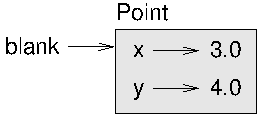
\includegraphics[scale=0.8]{figs/point.pdf}}
\caption{แผนภาพออบเจ๊คต์}
\label{fig.point}
\end{figure}

%The variable {\tt blank} refers to a Point object, which
%contains two attributes.  Each attribute refers to a
%floating-point number.

ตัวแปร {\tt blank} อ้างถึงออบเจ๊คต์ Point ซึ่งบรรจุสองแอตทริบิวต์ แต่ละแอตทริบิวต์อ้างอิงถึงตัวเลขทศนิยมอย่างละตัว

%You can read the value of an attribute using the same syntax:
เราสามารถอ่านค่าของแอตทริบิวต์แต่ละตัวด้วยวิธีการเดียวกัน

\begin{verbatim}
>>> blank.y
4.0
>>> x = blank.x
>>> x
3.0
\end{verbatim}
%
%The expression {\tt blank.x} means, ``Go to the object {\tt blank}
%refers to and get the value of {\tt x}.''  In the example, we assign that
%value to a variable named {\tt x}.  There is no conflict between
%the variable {\tt x} and the attribute {\tt x}.

นิพจน์ {\tt blank.x} หมายถึง ``ไปยังตำแหน่งที่อ้างถึงโดยออบเจ๊คต์ {\tt blank} และอ่านค่าของแอตทริบิวต์ {\tt x}'' 
ในตัวอย่างจะเห็นว่า มีการกำหนดค่าให้กับตัวแปร {\tt x} ซึ่งไม่ทำให้เกิดการขัดแย้งระหว่างตัวแปร {\tt x} และแอตทริบิวต์ {\tt x} แต่อย่างใด

%You can use dot notation as part of any expression.  For example:
คุณสามารถใช้สัญกรณ์จุดเป็นส่วนหนึ่งของนิพจน์ใดๆ ได้ ตัวอย่างเช่น

\begin{verbatim}
>>> '(%g, %g)' % (blank.x, blank.y)
'(3.0, 4.0)'
>>> distance = math.sqrt(blank.x**2 + blank.y**2)
>>> distance
5.0
\end{verbatim}
%
%You can pass an instance as an argument in the usual way.
%For example:
เราสามารถส่งผ่านอินสแตนซ์เป็นอาร์กูเมนต์ได้ตามปกติ ตัวอย่างเช่น
\index{instance!as argument}
\index{อินสแตนซ์!เป็นอาร์กูเมนต์}

\begin{verbatim}
def print_point(p):
    print('(%g, %g)' % (p.x, p.y))
\end{verbatim}
%
%\verb"print_point" takes a point as an argument and displays it in
%mathematical notation.  To invoke it, you can pass {\tt blank} as
%an argument:

\verb"print_point" รับจุดหนึ่งจุดเข้ามาเป็นอาร์กูเมนต์แล้วแสดงค่าแบบสัญลักษณ์ทางคณิตศาสตร์ จึงสามารถเรียกใช้โดยส่งผ่าน {\tt blank} เป็นอาร์กูเมนต์ได้

\begin{verbatim}
>>> print_point(blank)
(3.0, 4.0)
\end{verbatim}
%
%Inside the function, {\tt p} is an alias for {\tt blank}, so if
%the function modifies {\tt p}, {\tt blank} changes.

ภายในฟังก์ชัน {\tt p} เป็นสมนามของ {\tt blank} ดังนั้นถ้าฟังก์ชันมีการแก้ไขค่าของ {\tt p} ก็จะส่งผลต่อ {\tt blank} เช่นกัน
\index{aliasing}
\index{สมนาม}

%As an exercise, write a function called \verb"distance_between_points"
%that takes two Points as arguments and returns the distance between
%them.

เพื่อเป็นการฝึก ให้เขียนฟังก์ชันชื่อ  \verb"distance_between_points" ซึ่งรับจุดสองจุดเป็นอาร์กูเมนต์และให้ค่าออกมาเป็นระยะห่างระหว่างสองจุดนั้น

\section{รูปสี่เหลี่ยม} % (Rectangles)}
\label{rectangles}

Sometimes it is obvious what the attributes of an object should be,
but other times you have to make decisions.  For example, imagine you
are designing a class to represent rectangles.  What attributes would
you use to specify the location and size of a rectangle?  You can
ignore angle; to keep things simple, assume that the rectangle is
either vertical or horizontal.
บางครั้งก็มีความชัดเจนว่าอะไรควรเป็นแอตทริบิวต์ของออบเจ๊คต์ แต่ในบางคราวเราจะต้องตัดสินใจ ตัวอย่างเช่น 
ลองจินตนาการว่าเรากำลังออกแบบคลาสสำหรับรูปสี่เหลี่ยม อะไรเป็นแอตทริบิวต์ที่เราจะใช้เพื่อระบุตำแหน่งที่ตั้งและขนาดของรูปสี่เหลี่ยม? 
เราสามารถที่จะละเลยเรื่องของมุมเพื่อให้ง่ายขึ้นโดยสมมติว่ามีเฉพาะสี่เหลี่ยมในแนวตั้งและแนวนอน

\index{representation}
\index{การแทน}

%There are at least two possibilities: 

มีอย่างน้อยสองแนวทางที่เป็นไปได้

\begin{itemize}

%\item You could specify one corner of the rectangle
%(or the center), the width, and the height.
\item เราสามารถระบุมุมใดมุมหนึ่ง (หรือจุดศูนย์กลาง) ความกว้าง และความยาว

%\item You could specify two opposing corners.
\item เราสามารถระบุคู่จุดมุมตรงข้าม

\end{itemize}

%At this point it is hard to say whether either is better than
%the other, so we'll implement the first one, just as an example.

ณ จุดนี้ ยังเป็นการยากที่จะบอกว่าวิธีการไหนจะเป็นวิธีการที่ดีกว่าวิธีอื่น ดังนั้นเราจะลองทำตามวิธีแรกเพื่อเป็นตัวอย่าง

\index{Rectangle class}
\index{class!Rectangle}
\index{คลาสรูปสี่เหลี่ยม}
\index{คลาส!รูปสี่เหลี่ยม}

Here is the class definition:
นี่เป็นนิยามของคลาสดังกล่าว

\begin{verbatim}
class Rectangle:
    """Represents a rectangle. 

    attributes: width, height, corner.
    """
\end{verbatim}
%
%The docstring lists the attributes:  {\tt width} and
%{\tt height} are numbers; {\tt corner} is a Point object that
%specifies the lower-left corner.

ด็อกสตริงได้ระบุรายการแอตทริบิวต์ไว้ด้วยคือ {\tt width} และ {\tt height} เป็นตัวเลข 
ส่วน {\tt corner} เป็นออบเจ๊คต์ Point ที่ใช้ระบุตำแหน่งของมุมซ้ายล่าง

%To represent a rectangle, you have to instantiate a Rectangle
%object and assign values to the attributes:
เพื่อให้ได้ตัวแทนของรูปสี่เหลี่ยมหนึ่งรูป เราจะต้องสร้างอินสแตนซ์ของคลาส Rectangle และกำหนดค่าต่างๆ ให้กับแอตทริบิวต์ เช่น

\begin{verbatim}
box = Rectangle()
box.width = 100.0
box.height = 200.0
box.corner = Point()
box.corner.x = 0.0
box.corner.y = 0.0
\end{verbatim}
%
%The expression {\tt box.corner.x} means,
%``Go to the object {\tt box} refers to and select the attribute named
%{\tt corner}; then go to that object and select the attribute named
%{\tt x}.''

นิพจน์ {\tt box.corner.x} หมายถึง
``ไปยังตำแหน่งที่ออบเจ๊คต์ {\tt box} อ้างถึงและเลือกแอตทริบิวต์ชื่อว่า {\tt corner} ซึ่งจะเป็นการไปยังออบเจ๊คต์นั้นและเลือกแอตทริบิวต์ชื่อ {\tt x}''

\begin{figure}
\centerline
{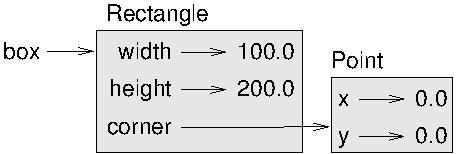
\includegraphics[scale=0.8]{figs/rectangle.pdf}}
\caption{แผนภาพออบเจ๊คต์}
\label{fig.rectangle}
\end{figure}


%Figure shows the state of this object.
%An object that is an attribute of another object is {\bf embedded}.

รูปที่~\ref{fig.rectangle} แสดงสถานะของออบเจ๊คต์ที่ได้ ออบเจ๊คต์ที่ถูกกำหนดเป็นแอตทริบิวต์ของออบเจ๊คต์อื่นจะ {\bf ฝังตัว} อยู่ภายในอีกที

\index{state diagram}
\index{diagram!state}
\index{object diagram}
\index{diagram!object}
\index{embedded object}
\index{object!embedded}
\index{แผนภาพสถานะ}
\index{แผนภาพ!สถานะ}
\index{แผนภาพออบเจ๊คต์}
\index{แผนภาพ!ออบเจ๊คต์}
\index{ออบเจ๊คต์ฝังตัว}
\index{ออบเจ๊คต์!ฝังตัว}


\section{อิสแสตนซ์เป็นค่าคืนกลับ} % (Instances as return values)}
\index{instance!as return value}
\index{return value}
\index{อินสแตนซ์!เป็นค่าคืนกลับ}
\index{ค่าคืนกลับ}

%Functions can return instances.  For example, \verb"find_center"
%takes a {\tt Rectangle} as an argument and returns a {\tt Point}
%that contains the coordinates of the center of the {\tt Rectangle}:

ฟังก์ชันสามารถส่งค่าออกมาเป็นอินสแตนซ์ได้ ตัวอย่างเช่น ฟังก์ชัน \verb"find_center" รับอาร์กูเมนต์เป็นออบเจ๊คต์ {\tt Rectangle} 
แล้วให้ค่าออกมาเป็นอินสแตนซ์ของ {\tt Point} ที่มีพิกัดตำแหน่งกึ่งกลางของรูปสี่เหลี่ยม

\begin{verbatim}
def find_center(rect):
    p = Point()
    p.x = rect.corner.x + rect.width/2
    p.y = rect.corner.y + rect.height/2
    return p
\end{verbatim}
%
%Here is an example that passes {\tt box} as an argument and assigns
%the resulting Point to {\tt center}:

นี่เป็นตัวอย่างการส่ง {\tt box} เป็นอาร์กูเมนต์และกำหนดค่าผลลัพธ์ซึ่งเป็นอินสแตนซ์ Point ให้กับ {\tt center}

\begin{verbatim}
>>> center = find_center(box)
>>> print_point(center)
(50, 100)
\end{verbatim}
%

\section{ออบเจ๊คต์เป็นชนิดข้อมูลที่เปลี่ยนแปลงได้} % (Objects are mutable)}
\index{object!mutable}
\index{mutability}
\index{ออบเจ๊คต์!เปลี่ยนแปลงได้}
\index{ความเปลี่ยนแปลงได้}

%You can change the state of an object by making an assignment to one of
%its attributes.  For example, to change the size of a rectangle
%without changing its position, you can modify the values of {\tt width} and {\tt height}:

เราสามารถเปลี่ยนแปลงสถานะของออบเจ๊คต์ได้ด้วยการกำหนดค่าใหม่ให้กับแอตทริบิวต์ของออบเจ๊คต์
ตัวอย่างเช่น การเปลี่ยนขนาดของรูปสี่เหลี่ยมโดยไม่ย้ายตำแหน่ง สามารถทำได้โดยการแก้ไขค่าของ {\tt width} และ {\tt height}

\begin{verbatim}
box.width = box.width + 50
box.height = box.height + 100
\end{verbatim}
%
%You can also write functions that modify objects.  For example,
%\verb"grow_rectangle" takes a Rectangle object and two numbers,
%{\tt dwidth} and {\tt dheight}, and adds the numbers to the
%width and height of the rectangle:

เราสามารถเขียนฟังก์ชันเพื่อแก้ไขออบเจ๊คต์ ตัวอย่างเช่น ฟังก์ชัน \verb"grow_rectangle" 
ซึ่งรับออบเจ๊คต์ Rectangle และตัวเลขอีกสองตัวคือ {\tt dwidth} และ {\tt dheight} สำหรับใช้บวกเพิ่มให้กับความกว้างและความสูงของรูปสี่เหลี่ยม


\begin{verbatim}
def grow_rectangle(rect, dwidth, dheight):
    rect.width += dwidth
    rect.height += dheight
\end{verbatim}
%
%Here is an example that demonstrates the effect:
นี่คือตัวอย่างที่แสดงให้เห็นถึงผลที่ได้

\begin{verbatim}
>>> box.width, box.height
(150.0, 300.0)
>>> grow_rectangle(box, 50, 100)
>>> box.width, box.height
(200.0, 400.0)
\end{verbatim}
%
%Inside the function, {\tt rect} is an
%alias for {\tt box}, so when the function modifies {\tt rect}, 
%{\tt box} changes.

{\tt rect} ที่อยู่ภายในฟังก์ชันเป็นสมนามของ {\tt box} ดังนั้นเมื่อใดที่ฟังก์ชันมีการแก้ไขค่าของ {\tt rect} ค่าของ {\tt box} ก็จะเปลี่ยนตาม

%As an exercise, write a function named \verb"move_rectangle" that takes
%a Rectangle and two numbers named {\tt dx} and {\tt dy}.  It
%should change the location of the rectangle by adding {\tt dx}
%to the {\tt x} coordinate of {\tt corner} and adding {\tt dy}
%to the {\tt y} coordinate of {\tt corner}.

เพื่อเป็นการฝึก ให้เขียนฟังก์ชันชื่อว่า \verb"move_rectangle" ซึ่งรับอาร์กูเมนต์เป็นออบเจ๊คต์ Rectangle 
และตัวเลขอีกสองจำนวนคือ {\tt dx} และ {\tt dy} ให้ฟังก์ชันทำการย้ายตำแหน่งของสี่เหลี่ยมด้วยบวกเพิ่ม 
{\tt dx} ให้กับพิกัด {\tt x} ของ {\tt corner} และบวกเพิ่ม {\tt dy} ให้กับพิกัด {\tt y} ของ {\tt corner}


\section{การทำสำเนา} % (Copying)}
\label{copying}
\index{aliasing}
\index{สมนาม}

%Aliasing can make a program difficult to read because changes
%in one place might have unexpected effects in another place.
%It is hard to keep track of all the variables that might refer
%to a given object.

การมีสมนามทำให้การทำความเข้าใจโปรแกรมทำได้ยาก เนื่องจากการเปลี่ยนแปลงค่าในที่หนึ่งอาจส่งผลกระทบอย่างคาดไม่ถึงกับอีกที่หนึ่ง 
ซึ่งจะเป็นการยากที่จะติดตามค่าของทุกตัวแปรที่มีการอ้างถึงออบเจ๊คต์ที่กำหนด

\index{copying objects}
\index{object!copying}
\index{copy module}
\index{module!copy}
\index{การทำสำเนาออบเจ๊คต์}
\index{ออบเจ๊คต์!การทำสำเนา}
\index{โมดูลสำเนา}
\index{โมดูล!สำเนา}

%Copying an object is often an alternative to aliasing.
%The {\tt copy} module contains a function called {\tt copy} that
%can duplicate any object:

การทำสำเนาออบเจ๊คต์เป็นอีกทางเลือกแทนการทำสมนาม โมดูล {\tt copy} มีฟังก์ชันชื่อว่า {\tt copy} ซึ่งสามารถสร้างสำเนาของออบเจ๊คต์ใดก็ได้

\begin{verbatim}
>>> p1 = Point()
>>> p1.x = 3.0
>>> p1.y = 4.0

>>> import copy
>>> p2 = copy.copy(p1)
\end{verbatim}
%
%{\tt p1} and {\tt p2} contain the same data, but they are
%not the same Point.

{\tt p1} และ {\tt p2} มีข้อมูลบรรจุภายในเหมือนกัน แต่เป็นคนละออบเจ๊คต์

\begin{verbatim}
>>> print_point(p1)
(3, 4)
>>> print_point(p2)
(3, 4)
>>> p1 is p2
False
>>> p1 == p2
False
\end{verbatim}
%
%The {\tt is} operator indicates that {\tt p1} and {\tt p2} are not the
%same object, which is what we expected.  But you might have expected
%{\tt ==} to yield {\tt True} because these points contain the same
%data.  In that case, you will be disappointed to learn that for
%instances, the default behavior of the {\tt ==} operator is the same
%as the {\tt is} operator; it checks object identity, not object
%equivalence.  That's because for programmer-defined types, Python doesn't
%know what should be considered equivalent.  At least, not yet.

ตัวดำเนินการ {\tt is} แสดงให้เห็นชัดว่า {\tt p1} และ {\tt p2} ไม่ใช่ออบเจ๊คต์เดียวกันเป็นไปตามที่เราคาดหวัง 
แต่เราอาจจะคาดหวังว่าตัวดำเนินการ {\tt ==} ให้ผลลัพธ์เป็น {\tt True} เนื่องจากทั้งสองจุดนี้มีข้อมูลที่เหมือนกัน 
ในกรณีนี้คุณอาจจะผิดหวังที่ได้รู้ว่า สำหรับอินสแตนซ์แล้วพฤติกรรมเริ่มต้นของตัวดำเนินการ {\tt ==} ให้ผลเหมือนกับตัวดำเนินการ {\tt is} 
ซึ่งจะตรวจสอบว่าเป็นออบเจ๊คต์อันเดียวกันหรือไม่ ไม่ใช่ตรวจสอบว่ามีความเท่าเทียมกันหรือไม่ 
ทั้งนี้เป็นเพราะว่าสำหรับชนิดข้อมูลที่ผู้เขียนโปรแกรมกำหนดขึ้นเองแล้วไพธอนไม่รู้ว่าควรจะตรวจสอบความเท่ากันอย่างไร อย่างน้อยก็ยัง

\index{is operator}
\index{operator!is}
\index{identity}
\index{equivalence}
\index{ตัวดำเนินการ is}
\index{ตัวดำเนินการ!is}
\index{อันเดียวกัน}
\index{ความเท่าเทียมกัน}

If you use {\tt copy.copy} to duplicate a Rectangle, you will find
that it copies the Rectangle object but not the embedded Point.

ถ้าเราใช้ {\tt copy.copy} เพื่อสำเนาออบเจ๊คต์ Rectangle เราจะพบว่ามีการสำเนาเฉพาะ Rectangle แต่จะไม่สำเนาออบเจ๊คต์ฝังตัว Point
\index{ออบเจ๊คต์ฝังตัว!การทำสำเนา}

\begin{verbatim}
>>> box2 = copy.copy(box)
>>> box2 is box
False
>>> box2.corner is box.corner
True
\end{verbatim}

\begin{figure}
\centerline
{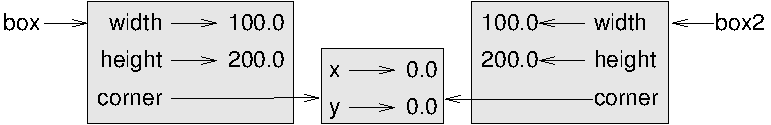
\includegraphics[scale=0.8]{figs/rectangle2.pdf}}
\caption{แผนภาพออบเจ๊คต์}
\label{fig.rectangle2}
\end{figure}

%Figure~\ref{fig.rectangle2} shows what the object diagram looks like.
%\index{state diagram}
%\index{diagram!state}
%\index{object diagram}
%\index{diagram!object}
%This operation is called a {\bf shallow copy} because it copies the
%object and any references it contains, but not the embedded objects.


รูปที่~\ref{fig.rectangle2} แสดงแผนภาพออบเจ๊คต์ให้เห็นว่ามีลักษณะอย่างไร 
\index{state diagram}
\index{diagram!state}
\index{object diagram}
\index{diagram!object}
\index{แผนภาพสถานะ}
\index{แผนภาพ!สถานะ}
\index{แผนภาพออบเจ๊คต์}
\index{แผนภาพ!ออบเจ๊คต์}
การทำงานเช่นนี้เรียกได้ว่าเป็น {\bf การสำเนาตื้น (shallow copy)} เนื่องจากทำการสำเนาเฉพาะตัวออบเจ๊คต์และทุกการอ้างอิง แต่ไม่สำเนาออบเจ๊คต์ที่ฝังอยู่ในออบเจ๊คต์นั้น
\index{shallow copy}
\index{copy!shallow}
\index{การสำเนาตื้น}

%For most applications, this is not what you want.  In this example,
%invoking \verb"grow_rectangle" on one of the Rectangles would not
%affect the other, but invoking \verb"move_rectangle" on either would
%affect both!  This behavior is confusing and error-prone.

สำหรับแอปพลิเคชันส่วนใหญ่ไม่ได้ต้องการผลลัพธ์เช่นนี้ ในตัวอย่างนี้การเรียกใช้  \verb"grow_rectangle" 
กับออบเจ๊คต์ Rectangle ใดจะไม่สร้างผลกระทบต่อออบเจ๊คต์อื่น 
แต่ถ้าเรียกใช้ \verb"move_rectangle" จะส่งผลกระทบทั้งคู่ พฤติกรรมเช่นนี้สร้างความสับสนและมีข้อผิดพลาดง่าย
\index{deep copy}
\index{copy!deep}
\index{การสำเนาลึก}

%Fortunately, the {\tt copy} module provides a method named {\tt deepcopy} that copies not only the object but also 
%the objects it refers to, and the objects {\em they} refer to,
%and so on.
%You will not be surprised to learn that this operation is
%called a {\bf deep copy}.

โชคดีที่โมดูล {\tt copy} ได้เตรียมเมธอดชื่อ {\tt deepcopy} ซึ่งคัดลอกไม่เฉพาะออบเจ๊คต์ที่ระบุแต่ยังคัดลอกรวมไปถึงออบเจ๊คต์ที่ถูกอ้างถึงและออบเจ๊คต์อื่นที่ถูกอ้างถึงด้วย {\em ออบเจ๊คต์เหล่านั้น} ไปเรื่อยๆ 
จึงไม่น่าแปลกใจที่กระบวนการนี้เรียกว่า {\bf การสำเนาลึก (deep copy)}
\index{deepcopy function}
\index{function!deepcopy}
\index{ฟังก์ชัน!สำเนาลึก}

\begin{verbatim}
>>> box3 = copy.deepcopy(box)
>>> box3 is box
False
>>> box3.corner is box.corner
False
\end{verbatim}
%
%{\tt box3} and {\tt box} are completely separate objects.

{\tt box3} และ {\tt box} เป็นคนละออบเจ๊คต์ที่แยกจากกันอย่างสมบูรณ์

%As an exercise, write a version of \verb"move_rectangle" that creates and
%returns a new Rectangle instead of modifying the old one.

เพื่อเป็นการฝึก ให้เขียนฟังก์ชัน \verb"move_rectangle" อีกเวอร์ชันที่สร้างออบเจ๊คต์ Rectangle และให้ค่าออกมาเป็นออบเจ๊คต์ใหม่ แทนการแก้ไขออบเจ๊คต์เดิม

\section{การดีบัก}
\label{hasattr}
\index{debugging}
\index{การดีบัก}

%When you start working with objects, you are likely to encounter
%some new exceptions.  If you try to access an attribute
%that doesn't exist, you get an {\tt AttributeError}:

เมื่อเราเริ่มทำงานกับออบเจ๊คต์ เรามีแนวโน้มที่จะพบเอ็กเซ็ปชั่นใหม่ๆ ถ้าเราพยายามเข้าถึงแอตทริบิวต์ที่ไม่มีอยู่จริง เราจะพบเอ็กเซ็ปชั่น {\tt AttributeError}

\index{exception!AttributeError}
\index{AttributeError}
\index{เอ็กเซ็ปชั่น!AttributeError}


\begin{verbatim}
>>> p = Point()
>>> p.x = 3
>>> p.y = 4
>>> p.z
AttributeError: Point instance has no attribute 'z'
\end{verbatim}
%
%If you are not sure what type an object is, you can ask:

ถ้าเราไม่แน่ใจว่าออบเจ๊คต์นั้นเป็นชนิดใด เราสามารถสอบถาม
\index{type function}
\index{function!type}
\index{ฟังก์ชัน type}
\index{ฟังก์ชัน!type}

\begin{verbatim}
>>> type(p)
<class '__main__.Point'>
\end{verbatim}
%
%You can also use {\tt isinstance} to check whether an object
%is an instance of a class:
เรายังสามารถใช้ {\tt isinstance} เพื่อตรวจสอบว่าออบเจ๊คต์นั้นเป็นอินสแตนซ์ของคลาสใดคลาสหนึ่งหรือไม่
\index{isinstance function}
\index{function!isinstance}
\index{ฟังก์ชัน isinstance}
\index{ฟังก์ชัน!isinstance}

\begin{verbatim}
>>> isinstance(p, Point)
True
\end{verbatim}
%
%If you are not sure whether an object has a particular attribute,
%you can use the built-in function {\tt hasattr}:

ถ้าเราไม่แน่ใจว่าออบเจ๊คต์หนึ่งมีแอตทริบิวต์ที่สนใจหรือไม่ เราสามารถใช้ฟังก์ชัน {\tt hasattr} ตรวจสอบได้

\index{hasattr function}
\index{function!hasattr}
\index{ฟังก์ชัน hasattr}
\index{ฟังก์ชัน!hasattr}

\begin{verbatim}
>>> hasattr(p, 'x')
True
>>> hasattr(p, 'z')
False
\end{verbatim}
%
%The first argument can be any object; the second argument is a {\em
%string} that contains the name of the attribute.

อาร์กูเมนต์แรกคือออบเจ๊คต์ใดๆ อาร์กูเมนต์ที่สองเป็น {\em สตริง} ที่มีชื่อของแอตทริบิวต์ที่ต้องการทราบ

\index{attribute}
\index{แอตทริบิวต์}

%You can also use a {\tt try} statement to see if the object has the
%attributes you need:

นอกจากนี้เรายังสามารถใช้คำสั่ง {\tt try} เพื่อหาดูว่าออบเจ๊คต์นั้นมีแอตทริบิวต์ที่เราต้องการหรือไม่

\index{try statement}
\index{statement!try}
\index{คำสั่ง try}
\index{คำสั่ง!try}

\begin{verbatim}
try:
    x = p.x
except AttributeError:
    x = 0
\end{verbatim}

%This approach can make it easier to write functions that work with
%different types; more on that topic is
%coming up in Section~\ref{polymorphism}.

วิธีนี้สามารถช่วยทำให้การเขียนฟังก์ชันเพื่อทำงานกับหลากหลายชนิดข้อมูลได้ ดูรายละเอียดเพิ่มเติมในหัวข้อ~\ref{polymorphism} 

%\section{Glossary}
\section{อภิธานศัพท์}

\begin{description}

%\item[class:] A programmer-defined type.  A class definition creates a new
%class object.
\item[คลาส (class):] ชนิดข้อมูลที่ผู้เขียนโปรแกรมกำหนดเอง การประกาศคลาสจะสร้างคลาสออบเจ๊คต์ใหม่ขึ้น
\index{class}
\index{programmer-defined type}
\index{type!programmer-defined}
\index{คลาส}
\index{ชนิดข้อมูลที่ผู้เขียนโปรแกรมกำหนดเอง}
\index{ชนิดข้อมูล!ผู้เขียนโปรแกรมกำหนดเอง}

%\item[class object:] An object that contains information about a
%programmer-defined type.  The class object can be used to create instances
%of the type.

\item[คลาสออบเจ๊คต์ (class object):] ออบเจ๊คต์ที่มีรายละเอียดของชนิดข้อมูลที่ผู้เขียนโปรแกรมกำหนดขึ้นเอง
คลาสออบเจ๊คต์สามารถใช้สร้างอินแสตนซ์ของชนิดข้อมูลนั้นได้
\index{class object}
\index{object!class}
\index{คลาสออบเจ๊คต์}
\index{ออบเจ๊คต์!คลาส}

%\item[instance:] An object that belongs to a class.
\item[อินสแตนซ์ (instance):] ออบเจ๊คต์ที่เป็นสังกัดของคลาส
\index{instance}
\index{อินสแตนซ์}

%\item[instantiate:] To create a new object.
\item[สร้างอินสแตนซ์ (instantiate):] การสร้างออบเจ๊คต์ใหม่
\index{สร้างอินสแตนซ์}

%\item[attribute:] One of the named values associated with an object.
\item[แอตทริบิวต์ (attribute):] ชื่อพร้อมกับค่าซึ่งผูกอยู่กับออบเจ๊คต์
\index{attribute!instance}
\index{instance attribute}
\index{แอตทริบิวต์!อินสแตนซ์}
\index{อินสแตนซ์แอตทริบิวต์}

%\item[embedded object:] An object that is stored as an attribute
%of another object.

\item[ออบเจ๊คต์ฝังตัว (embedded object):] ออบเจ๊คต์ที่ถูกเก็บเป็นแอตทริบิวต์ของออบเจ๊คต์อื่น
\index{embedded object}
\index{object!embedded}
\index{ออบเจ๊คต์ฝังตัว}

%\item[shallow copy:] To copy the contents of an object, including
%any references to embedded objects;
%implemented by the {\tt copy} function in the {\tt copy} module.

\item[สำเนาตื้น (shallow copy):] การสำเนาข้อมูลภายในออบเจ๊คต์รวมถึงแอตทริบิวต์ที่เป็นอ้างอิงไปยังออบเจ๊คต์ฝังตัว
ทำได้โดยการเรียกใช้ฟังก์ชัน {\tt copy} ที่อยู่ในโมดูล {\tt copy}
\index{shallow copy}
\index{สำเนาตื้น}

%\item[deep copy:] To copy the contents of an object as well as any
%embedded objects, and any objects embedded in them, and so on;
%implemented by the {\tt deepcopy} function in the {\tt copy} module.

\item[สำเนาลึก (deep copy):] การสำเนาข้อมูลภายในออบเจ๊คต์รวมทั้งข้อมูลของออบเจ๊คต์ที่เป็นออบเจ๊คต์ฝังตัวตลอดจนข้อมูลออบเจ๊คต์อื่นที่ถูกอ้างอิงด้วยออบเจ๊คต์ฝังตัวเหล่านั้นไปเรื่อยๆ 
ทำได้โดยการเรียกใช้ฟังก์ชัน {\tt deepcopy} ที่อยู่ในโมดูล {\tt copy}
\index{deep copy}
\index{สำเนาลึก}

%\item[object diagram:] A diagram that shows objects, their
%attributes, and the values of the attributes.

\item[แผนภาพออบเจ๊คต์ (object diagram):] แผนภาพที่มีการแสดงออบเจ๊คต์กับแอตทริบิวต์ภายในและค่าของแต่ละแอตทริบิวต์
\index{object diagram}
\index{diagram!object}
\index{แผนภาพออบเจ๊คต์}
\index{แผนภาพ!ออบเจ๊คต์}

\end{description}


%\section{Exercises}
\section{แบบฝึกหัด}

\begin{exercise}

%Write a definition for a class named {\tt Circle} with attributes
%{\tt center} and {\tt radius}, where {\tt center} is a Point object
%and radius is a number.

เขียนนิยามของคลาสชื่อ {\tt Circle} ที่มีแอตทริบิวต์ {\tt center} และ {\tt radius} กำหนดให้ {\tt center} เป็นออบเจ๊คต์ของ Point และให้ radius เป็นตัวเลข

%Instantiate a Circle object that represents a circle with its center
%at $(150, 100)$ and radius 75.

สร้างอินสแตนซ์ของ Circle ซึ่งเป็นตัวแทนของวงกลมซึ่งมีจุดศูนย์กลางอยู่ที่ $(150, 100)$ รัศมี 75 หน่วย

%Write a function named \verb"point_in_circle" that takes a Circle and
%a Point and returns True if the Point lies in or on the boundary of
%the circle.
เขียนฟังก์ชันชื่อ \verb"point_in_circle" ซึ่งรับออบเจ๊คต์ Circle และ Point แล้วให้ค่าคืนกลับเป็น True ถ้าจุดนั้นอยู่ภายในหรือบนขอบเขตของวงกลม


%Write a function named \verb"rect_in_circle" that takes a Circle and a
%Rectangle and returns True if the Rectangle lies entirely in or on the boundary
%of the circle.
เขียนฟังก์ชันชื่อ \verb"rect_in_circle" ซึ่งรับออบเจ๊คต์ Circle และ Rectangle แล้วให้ค่าคืนกลับเป็น True ถ้ารูปสี่เหลี่ยมนั้นอยู่ภายในหรือบนขอบเขตของวงกลม


%Write a function named \verb"rect_circle_overlap" that takes a Circle
%and a Rectangle and returns True if any of the corners of the Rectangle fall
%inside the circle.  Or as a more challenging version, return True if
%any part of the Rectangle falls inside the circle.

เขียนฟังก์ชันชื่อ \verb"rect_circle_overlap" ซึ่งรับออบเจ๊คต์ Circle และ Rectangle 
แล้วให้ค่าคืนกลับเป็น True ถ้ามุมใดมุมหนึ่งของสี่เหลี่ยมอยู่ภายในวงกลม หรือเขียนรุ่นที่ท้าทายมากขึ้นซึ่งจะให้ค่าออกมาเป็น True 
ถ้าส่วนใดส่วนหนึ่งของรูปสี่เหลี่ยมอยู่ภายในวงกลม


%Solution: \url{http://thinkpython2.com/code/Circle.py}.
เฉลย: \url{http://thinkpython2.com/code/Circle.py}.

\end{exercise}


\begin{exercise}

%Write a function called \verb|draw_rect| that takes a Turtle object
%and a Rectangle and uses the Turtle to draw the Rectangle.  See
%Chapter~\ref{turtlechap} for examples using Turtle objects.

เขียนฟังก์ชันชื่อ \verb|draw_rect| ซึ่งรับออบเจ๊คต์  Turtle และ  Rectangle แล้วใช้ออบเจ๊คต์ Turtle 
ในการวาดรูปสี่เหลี่ยมโดยดูตัวอย่างการใช้งาน Turtle ในบทที่ ~\ref{turtlechap}

%Write a function called \verb|draw_circle| that takes a Turtle and
%a Circle and draws the Circle.
เขียนฟังก์ชันชื่อ \verb|draw_circle| ซึ่งรับออบเจ๊คต์ Turtle และ  Circle แล้ววาดรูปของวงกลมนั้น

โปรแกรมเฉลย: \url{http://thinkpython2.com/code/draw.py}.

\end{exercise}



\chapter{คลาสและฟังก์ชัน} % (Classes and functions)}
\label{time}

%Now that we know how to create new types, the next
%step is to write functions that take programmer-defined objects
%as parameters and return them as results.  In this chapter I
%also present ``functional programming style'' and two new
%program development plans.

ตอนนี้เราได้รู้วิธีการสร้างชนิดข้อมูลใหม่ ขั้นต่อไปเป็นการเขียนฟังก์ชันที่รับออบเจ๊คต์ชนิดผู้เขียนโปรแกรมกำหนดขึ้นเป็นพารามิเตอร์
และให้ค่าออกมาเป็นออบเจ๊คต์เหล่านั้น ในบทนี้ได้นำเสนอ ``การเขียนโปรแกรมเชิงฟังก์ชัน (functional programming style)'' และแผนการพัฒนาสองโปรแกรมใหม่


%Code examples from this chapter are available from
%\url{http://thinkpython2.com/code/Time1.py}.
%Solutions to the exercises are at
%\url{http://thinkpython2.com/code/Time1_soln.py}.

ตัวอย่างโปรแกรมของบทนี้สามารถดาวน์โหลดได้ที่ \url{http://thinkpython2.com/code/Time1.py}
ผลเฉลยสำหรับแบบฝึกหัดอยู่ที่ \url{http://thinkpython2.com/code/Time1_soln.py}

%\section{Time}
\section{เวลา} % (Time)}
\label{isafter}

%As another example of a programmer-defined type, we'll define a class
%called {\tt Time} that records the time of day.  The class definition
%looks like this: 
เช่นกันกับตัวอย่างอื่นของชนิดข้อมูลที่ผู้เขียนโปรแกรมกำหนดเอง เราจะประกาศคลาส {\tt Time} ซึ่งใช้บันทึกเวลาของวัน นิยามของคลาสมีลักษณะดังนี้
\index{programmer-defined type}
\index{type!programmer-defined} 
\index{Time class} 
\index{class!Time}
\index{ชนิดข้อมูลที่ผู้เขียนโปรแกรมกำหนดเอง}
\index{ชนิดข้อมูล!ผู้เขียนโปรแกรมกำหนดเอง} 
\index{คลาส Time} 
\index{คลาส!Time}

\begin{verbatim}
class Time:
    """Represents the time of day.
       
    attributes: hour, minute, second
    """
\end{verbatim}
%
%We can create a new {\tt Time} object and assign
%attributes for hours, minutes, and seconds:

เราสามารถสร้างออบเจ๊คต์ใหม่ของ {\tt Time} และกำหนดค่าของแอตทริบิวต์ชั่วโมง (hour) นาที (minute) และ วินาที (second)

\begin{verbatim}
time = Time()
time.hour = 11
time.minute = 59
time.second = 30
\end{verbatim}
%
%The state diagram for the {\tt Time} object looks like Figure~\ref{fig.time}.
แผนภาพสถานะของออบเจ๊คต์ {\tt Time} มีลักษณะดังแสดงในรูปที่~\ref{fig.time}
\index{state diagram}
\index{diagram!state}
\index{object diagram}
\index{diagram!object}
\index{แผนภาพสถานะ}
\index{แผนภาพ!สถานะ}
\index{แผนภาพออบเจ๊คต์}
\index{แผนภาพ!ออบเจ๊คต์}

%As an exercise, write a function called \verb|print_time| that takes a 
%Time object and prints it in the form {\tt hour:minute:second}.
%Hint: the format sequence \verb"'%.2d'" prints an integer using
%at least two digits, including a leading zero if necessary.

เพื่อเป็นการฝึก ให้เขียนฟังก์ชันชื่อ \verb|print_time| ซึ่งรับออบเจ๊คต์ Time 
และพิมพ์ค่าเวลาในรูปแบบ {\tt ชั่วโมง:นาที:วินาที}  
ข้อแนะนำคือ ใช้รูปแบบ \verb"'%.2d'" สำหรับพิมพ์ตัวเลขอย่างน้อยสองตำแหน่ง โดยจะเติมศูนย์ด้านหน้ากรณีค่าน้อยกว่าสิบ

%Write a boolean function called \verb"is_after" that
%takes two Time objects, {\tt t1} and {\tt t2}, and
%returns {\tt True} if {\tt t1} follows {\tt t2} chronologically and
%{\tt False} otherwise.  Challenge: don't use an {\tt if} statement.

เขียนฟังก์ชันบูลีนชื่อ \verb"is_after" ซึ่งรับออบเจ๊คต์ของ Time สองออบเจ๊คต์ {\tt t1} และ {\tt t2} 
แล้วให้ค่าออกมาเป็น {\tt True} ถ้าเวลา {\tt t1} ตามหลังเวลา {\tt t2} ตามลำดับเหตุการณ์ ไม่เช่นนั้นจะให้ค่าออกมาเป็น {\tt False}
ท้าทาย: ลองเขียนฟังก์ชันโดยไม่ใช้คำสั่ง {\tt if}

\begin{figure}
\centerline
{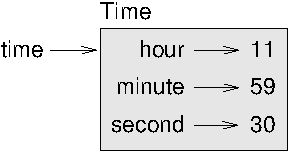
\includegraphics[scale=0.8]{figs/time.pdf}}
\caption{แผนภาพออบเจ๊คต์}
\label{fig.time}
\end{figure}


%\section{Pure functions}
\section{ฟังก์ชันบริสุทธิ์} % (Pure functions)}
\index{prototype and patch}
\index{development plan!prototype and patch}
\index{วิธีต้นแบบและเติมแต่ง}
\index{แผนการพัฒนา!วิธีต้นแบบและเติมแต่ง}


%In the next few sections, we'll write two functions that add time
%values.  They demonstrate two kinds of functions: pure functions and
%modifiers.  They also demonstrate a development plan I'll call {\bf
%  prototype and patch}, which is a way of tackling a complex problem
%by starting with a simple prototype and incrementally dealing with the
%complications.

ในหัวข้อถัดๆ ไป เราจะเขียนสองฟังก์ชันสำหรับบวกเวลาซึ่งแสดงรูปแบบการเขียนฟังก์ชันไว้สองแบบคือ 
แบบฟังก์ชันบริสุทธิ์ (pure function) และ แบบตัวดัดแปลง (modifier) และได้แสดงแผนการพัฒนาที่เรียกว่า วิธี
{\bf ต้นแบบและเติมแต่ง (prototype and patch)} ซึ่งเป็นวิธีการแก้ปัญหาที่ซับซ้อนโดยเริ่มจากต้นแบบอย่างง่าย 
และเพิ่มเติมการจัดการกับความซับซ้อนอย่างค่อยเป็นค่อยไป

%Here is a simple prototype of \verb"add_time":
นี่เป็นต้นแบบอย่างง่ายของฟังก์ชัน \verb"add_time"

\begin{verbatim}
def add_time(t1, t2):
    sum = Time()
    sum.hour = t1.hour + t2.hour
    sum.minute = t1.minute + t2.minute
    sum.second = t1.second + t2.second
    return sum
\end{verbatim}
%
%The function creates a new {\tt Time} object, initializes its
%attributes, and returns a reference to the new object.  This is called
%a {\bf pure function} because it does not modify any of the objects
%passed to it as arguments and it has no effect,
%like displaying a value or getting user input, 
%other than returning a value.

ภายในฟังก์ชันมีการสร้างออบเจ๊คต์ {\tt Time} ขึ้นใหม่ และกำหนดค่าตั้งต้นให้กับแอตทริบิวต์แล้วให้ค่าออกมาเป็นอ้างอิงไปยังออบเจ๊คต์ใหม่นั้น 
การทำงานเช่นนี้เรียกว่า {\bf ฟังก์ชันบริสุทธิ์} เนื่องจากไม่มีการแก้ไขค่าของออบเจ๊คต์ที่ถูกส่งเป็นอาร์กูเมนต์และไม่ได้รับผลกระทบใดเว้นแต่ค่าที่ให้ออกมา 
มีลักษณะเดียวกับฟังก์ชันสำหรับแสดงค่าหรือฟังก์ชันสำหรับรับอินพุตจากผู้ใช้
\index{pure function}
\index{function type!pure}
\index{ฟังก์ชันบริสุทธิ์}
\index{ชนิดฟังก์ชัน!บริสุทธิ์}

%To test this function, I'll create two Time objects: {\tt start}
%contains the start time of a movie, like {\em Monty Python and the
%Holy Grail}, and {\tt duration} contains the run time of the movie,
%which is one hour 35 minutes.

เพื่อการทดสอบฟังก์ชันจึงสร้างออบเจ๊คต์ของ Time ขึ้นมาสองออบเจ๊คต์ ออบเจ๊คต์ {\tt start} ใช้เก็บค่าเวลาเริ่มต้นของภาพยนต์ 
เช่นเรื่อง {\em ไพธอนยักษ์กับจอกศักดิ์สิทธิ์ (Monty Python and the Holy Grail)} และออบเจ๊คต์ {\tt duration} 
สำหรับเก็บค่าเวลาที่ใช้ในการฉายภาพยนต์ ซึ่งจะเป็น 1 ชั่วโมง 35 นาที
\index{Monty Python and the Holy Grail}
\index{ไพธอนยักษ์กับจอกศักดิ์สิทธิ์}

%\verb"add_time" figures out when the movie will be done.
ฟังก์ชัน \verb"add_time" จะหาว่าภาพยนต์ถูกฉายจบตอนไหน

\begin{verbatim}
>>> start = Time()
>>> start.hour = 9
>>> start.minute = 45
>>> start.second =  0

>>> duration = Time()
>>> duration.hour = 1
>>> duration.minute = 35
>>> duration.second = 0

>>> done = add_time(start, duration)
>>> print_time(done)
10:80:00
\end{verbatim}
%
%The result, {\tt 10:80:00} might not be what you were hoping
%for.  The problem is that this function does not deal with cases where the
%number of seconds or minutes adds up to more than sixty.  When that
%happens, we have to ``carry'' the extra seconds into the minute column
%or the extra minutes into the hour column.

ผลลัพธ์คือ {\tt 10:80:00} อาจจะไม่ใช่อย่างที่เราหวังไว้ ปัญหาคือ ฟังก์ชันไม่ได้จัดการกับกรณีจำนวนเวลาวินาทีและนาทีที่มีผลรวมเกิน 60 
เมื่อเกิดเหตุการณ์ดังกล่าวเราจะต้อง ``ทด'' เวลาส่วนเกินของวินาทีไปที่นาที และยกยอดนาทีส่วนเกินไปเพิ่มให้กับชั่วโมง
\index{carrying, addition with}
\index{การทด, บวกกับ}

%Here's an improved version:
นี่คือฟังก์ชันรุ่นที่ได้รับการปรับปรุง

\begin{verbatim}
def add_time(t1, t2):
    sum = Time()
    sum.hour = t1.hour + t2.hour
    sum.minute = t1.minute + t2.minute
    sum.second = t1.second + t2.second

    if sum.second >= 60:
        sum.second -= 60
        sum.minute += 1

    if sum.minute >= 60:
        sum.minute -= 60
        sum.hour += 1

    return sum
\end{verbatim}
%
%Although this function is correct, it is starting to get big.
%We will see a shorter alternative later.
แม้ว่าฟังก์ชันนี้จะถูกต้องแล้ว แต่ก็ค่อนข้างใหญ่ เราจะมาดูเวอร์ชันที่สั้นกว่านี้ในภายหลัง

%\section{Modifiers}
\section{ตัวดัดแปลง} % (Modifiers)}
\label{increment}
\index{modifier}
\index{function type!modifier}
\index{ตัวดัดแปลง}
\index{ชนิดฟังก์ชัน!ตัวดัดแปลง}

%Sometimes it is useful for a function to modify the objects it gets as
%parameters.  In that case, the changes are visible to the caller.
%Functions that work this way are called {\bf modifiers}.

ในบางครั้งก็ถือเป็นประโยชน์มากที่จะให้ฟังก์ชันแก้ไขค่าออบเจ๊คต์ที่รับมาเป็นพารามิเตอร์  
ในกรณีนั้นการเปลี่ยนแปลงสามารถรับรู้ได้ถึงตำแหน่งที่ฟังก์ชันถูกเรียกใช้ ฟังก์ชันที่ทำงานลักษณะนี้เรียกว่า ตัวดัดแปลง (modifiers)
\index{increment}
\index{การเพิ่มค่า}

%{\tt increment}, which adds a given number of seconds to a {\tt Time}
%object, can be written naturally as a
%modifier.  Here is a rough draft:

ฟังก์ชัน {\tt increment} ทำการบวกเพิ่มตัวเลขจำนวนวินาทีให้กับออบเจ๊คต์ {\tt Time} สามารถเขียนเป็นตัวดัดแปลงได้อย่างเป็นธรรมชาติ และนี่เป็นร่างคร่าวๆ

\begin{verbatim}
def increment(time, seconds):
    time.second += seconds

    if time.second >= 60:
        time.second -= 60
        time.minute += 1

    if time.minute >= 60:
        time.minute -= 60
        time.hour += 1
\end{verbatim}
%
%The first line performs the basic operation; the remainder deals
%with the special cases we saw before.

บรรทัดแรกทำหน้าที่บวกเพิ่มวินาที ส่วนที่เหลือเป็นการจัดการกับกรณีพิเศษที่เราเจอก่อนหน้านี้
\index{special case}
\index{กรณีพิเศษ}

%Is this function correct?  What happens if {\tt seconds}
%is much greater than sixty?  
ฟังก์ชันนี้ทำงานได้ถูกต้องหรือไม่? อะไรจะเกิดขึ้นถ้าค่าของ {\tt วินาที} มีค่ามากกว่า 60 มากๆ?


%In that case, it is not enough to carry once; we have to keep doing it
%until {\tt time.second} is less than sixty.  One solution is to
%replace the {\tt if} statements with {\tt while} statements.  That
%would make the function correct, but not very efficient.  As an
%exercise, write a correct version of {\tt increment} that doesn't
%contain any loops.

ในกรณีนั้น การทดค่าเพียงแค่ครั้งเดียวจะยังไม่เพียงพอ เราจะต้องทำซ้ำจนกว่าค่าของ {\tt time.second} จะน้อยกว่า 60 
แนวทางหนึ่งที่ทำได้คือ แทนที่คำสั่ง  {\tt if} ด้วยคำสั่ง {\tt while} จะทำให้การทำงานของฟังก์ชันถูกต้องแต่ก็ไม่ค่อยมีประสิทธิภาพนัก 
ทำเป็นแบบฝึกหัด คือ เขียนฟังก์ชัน {\tt increment} เวอร์ชันที่ถูกต้องแต่ไม่มีการทำงานแบบวนซ้ำ


%Anything that can be done with modifiers can also be done with pure
%functions.  In fact, some programming languages only allow pure
%functions.  There is some evidence that programs that use pure
%functions are faster to develop and less error-prone than programs
%that use modifiers.  But modifiers are convenient at times,
%and functional programs tend to be less efficient.

การทำงานทุกอย่างที่สามารถทำได้ด้วยตัวดัดแปลงจะสามารถทำด้วยฟังก์ชันบริสุทธิ์ได้เช่นกัน 
อันที่จริงภาษาเขียนโปรแกรมบางภาษาอนุญาตให้เขียนเฉพาะฟังก์ชันบริสุทธิ์ เนื่องจากมีความเชื่อว่า 
โปรแกรมที่ใช้เฉพาะฟังก์ชันบริสุทธิ์พัฒนาได้เร็วกว่าและมีข้อผิดพลาดน้อยกว่าโปรแกรที่ใช้ตัวดัดแปลง 
แต่หลายครั้งที่การใช้ตัวดัดแปลงมีความสะดวกสบายกว่า (และการใช้ฟังก์ชันมีแนวโน้มของประสิทธิภาพด้อยกว่า)


%In general, I recommend that you write pure functions whenever it is
%reasonable and resort to modifiers only if there is a compelling
%advantage.  This approach might be called a {\bf functional
%programming style}.

โดยทั่วไป ฉันแนะนำให้คุณเขียนฟังก์ชันบริสุทธิ์เมื่อใดก็ตามที่สมเหตุสมผล และใช้ตัวดัดแปลงเฉพาะเมื่อมีข้อได้เปรียบที่น่าสนใจเท่านั้น 
แนวทางนี้อาจเรียกว่ารูปแบบ {\bf การเขียนโปรแกรมเชิงฟังก์ชัน (functional programming style)}
\index{functional programming style}
\index{การเขียนโปรแกรมเชิงฟังก์ชัน}

%As an exercise, write a ``pure'' version of {\tt increment} that
%creates and returns a new Time object rather than modifying the
%parameter.

เพื่อเป็นการฝึก ให้เขียนฟังก์ชัน {\tt increment} ที่เป็นรุ่น ``บริสุทธิ์ (pure)'' 
ซึ่งจะสร้างออบเจ๊คต์ Time ขึ้นมาใหม่และให้ค่าคืนกลับเป็นออบเจ๊คต์นั้นแทนการไก้ไขค่าของพารามิเตอร์

%\section{Prototyping versus planning}
\section{การสร้างต้นแบบเทียบกับการวางแผน} % (Prototyping versus planning)}
\label{prototype}
\index{prototype and patch}
\index{development plan!prototype and patch}
\index{planned development}
\index{development plan!designed}
\index{วิธีต้นแบบและเติมแต่ง}
\index{แผนการพัฒนา!วิธีต้นแบบและเติมแต่ง}
\index{แผนการพัฒนา!ได้รับการออกแบบ}

%The development plan I am demonstrating is called ``prototype and
%patch''.  For each function, I wrote a prototype that performed the
%basic calculation and then tested it, patching errors along the
%way.

แผนการพัฒนาที่ผ่านมาถูกเรียกว่า ``วิธีต้นแบบและเติมแต่ง'' แต่ละฟังก์ชันถูกทำเป็นต้นแบบด้วยการทำงานพื้นฐานก่อน จากนั้นทดสอบและปรับแก้ข้อผิดพลาดที่เกิดขึ้นระหว่างใช้งาน

%This approach can be effective, especially if you don't yet have a
%deep understanding of the problem.  But incremental corrections can
%generate code that is unnecessarily complicated---since it deals with
%many special cases---and unreliable---since it is hard to know if you
%have found all the errors.

แนวทางนี้สามารถเป็นหนทางที่มีประสิทธิภาพ โดยเฉพาะในเวลาที่เรายังไม่มีความเข้าใจปัญหาอย่างลึกซึ้ง 
แต่การปรับเพิ่มการแก้ไขสามารถทำให้โค้ดมีความซับซ้อน เพราะต้องจัดการกับกรณีเฉพาะหลายกรณี และทำให้ไม่น่าเชื่อถือ 
เนื่องจากเป็นการยากที่จะรู้ได้ว่าเราเจอข้อผิดพลาดได้ครบทุกกรณี


%An alternative is {\bf designed development}, in which high-level
%insight into the problem can make the programming much easier.  In
%this case, the insight is that a Time object is really a three-digit
%number in base 60 (see \url{http://en.wikipedia.org/wiki/Sexagesimal}.)!  The
%{\tt second} attribute is the ``ones column'', the {\tt minute}
%attribute is the ``sixties column'', and the {\tt hour} attribute is
%the ``thirty-six hundreds column''.

อีกทางเลือกหนึ่งคือ {\bf การออกแบบแล้วพัฒนา (designed development)} ซึ่งมีการเข้าใจปัญหาในระดับสูงช่วยทำให้การเขียนโปรแกรมง่ายขึ้นมาก 
ในกรณีนี้ความเข้าใจระดับสูงคือ ออบเจ๊คต์ Time เป็นเลขฐาน 60 จำนวน 3 ตำแหน่ง !
(ดูข้อมูลเพิ่มเติม \url{http://en.wikipedia.org/wiki/Sexagesimal}) โดยมี{\tt วินาที}เป็นหลักหน่วย มี{\tt นาที}เป็นหลัก 60 และ{\tt ชั่วโมง}เป็นหลัก 3600
\index{sexagesimal}
\index{เลขฐานหกสิบ}

%When we wrote \verb"add_time" and {\tt increment}, we were effectively
%doing addition in base 60, which is why we had to carry from one
%column to the next.

เมื่อเราเขียนฟังก์ชัน \verb"add_time" และ {\tt increment} เราได้ทำการบวกในฐาน 60 
และนี่คือเหตุผลว่าทำไมเราจึงทดจากหลักหนึ่งไปยังหลักถัดไป
\index{carrying, addition with}
\index{การทด, บวกกับ}

%This observation suggests another approach to the whole problem---we
%can convert Time objects to integers and take advantage of the fact
%that the computer knows how to do integer arithmetic.  

จากข้อสังเกตนี้จึงได้แนวทางใหม่ที่สามารถจัดการปัญหาได้ทั้งหมด 
เนื่องจากเราสามารถแปลงเวลาให้เป็นจำนวนเต็มและใช้ความสามารถของคอมพิวเตอร์ช่วยบวกจำนวนเต็มให้

%Here is a function that converts Times to integers:

นี่คือฟังก์ชันที่แปลงเวลาเป็นจำนวนเต็ม

\begin{verbatim}
def time_to_int(time):
    minutes = time.hour * 60 + time.minute
    seconds = minutes * 60 + time.second
    return seconds
\end{verbatim}
%
%And here is a function that converts an integer to a Time
%(recall that {\tt divmod} divides the first argument by the second
%and returns the quotient and remainder as a tuple).

และนี่คือฟังก์ชันที่แปลงจำนวนเต็มเป็นเวลา (พึงระลึกว่าฟังก์ชัน {\tt divmod} 
หารอาร์กูเมนต์แรกด้วยอาร์กูเมนต์ที่สองแล้วให้ค่าออกมาเป็นผลหารและเศษในรูปของทูเพิล)
\index{divmod}

\begin{verbatim}
def int_to_time(seconds):
    time = Time()
    minutes, time.second = divmod(seconds, 60)
    time.hour, time.minute = divmod(minutes, 60)
    return time
\end{verbatim}
%
%You might have to think a bit, and run some tests, to convince
%yourself that these functions are correct.  One way to test them is to
%check that \verb"time_to_int(int_to_time(x)) == x" for many values of
%{\tt x}.  This is an example of a consistency check.

อาจจะต้องใช้เวลาคิดสักหน่อยหรือรันทดสอบเพื่อให้มั่นใจว่าฟังก์ชันนี้ทำงานได้ถูกต้อง  วิธีหนึ่งที่จะช่วยทดสอบได้คือ ตรวจสอบว่า
\verb"time_to_int(int_to_time(x)) == x" สำหรับหลายๆ ค่าของ {\tt x} นี่เป็นตัวอย่างของการตรวจสอบความสอดคล้อง
\index{consistency check}
\index{การตรวจสอบความสอดคล้อง}

%Once you are convinced they are correct, you can use them to 
%rewrite \verb"add_time":

และเมื่อมั่นใจแล้วว่าการทำงานนั้นถูกต้อง เราก็สามารถใช้คำสั่งเหล่านี้มาเขียนฟังก์ชัน \verb"add_time" ใหม่ได้ดังนี้

\begin{verbatim}
def add_time(t1, t2):
    seconds = time_to_int(t1) + time_to_int(t2)
    return int_to_time(seconds)
\end{verbatim}
%
%This version is shorter than the original, and easier to verify.  As
%an exercise, rewrite {\tt increment} using \verb"time_to_int" and
%\verb"int_to_time".

เวอร์ชันนี้สั้นกว่าเวอร์ชันก่อนหน้าและง่ายต่อการตรวจสอบ ให้ทำเป็นแบบฝึกหัด คือ เขียนฟังก์ชัน {\tt increment} ใหม่โดยใช้ฟังก์ชัน \verb"time_to_int" และ \verb"int_to_time" ช่วย


%In some ways, converting from base 60 to base 10 and back is harder
%than just dealing with times.  Base conversion is more abstract; our
%intuition for dealing with time values is better.

บางทีการแปลงค่าจากฐาน 60 เป็นฐาน 10 ไปและกลับก็ยากกว่าการจัดการกับเวลา การแปลงฐานเข้าใจได้ยากกว่า สัญชาตญาณของเราจึงบอกว่าการจัดการกับเวลาน่าจะเป็นวิธีที่ดีกว่า

%But if we have the insight to treat times as base 60 numbers and make
%the investment of writing the conversion functions (\verb"time_to_int"
%and \verb"int_to_time"), we get a program that is shorter, easier to
%read and debug, and more reliable.

แต่ถ้าเราเข้าใจได้อย่างถ่องแท้เรื่องการจัดการกับเลขฐาน 60 และได้ลงทุนเขียนฟังก์ชันการแปลงแล้ว (\verb"time_to_int" และ \verb"int_to_time") 
เราจะได้โปรแกรมที่สั้นกว่า ง่ายต่อการทำความเข้าใจและแก้ไข แถมยังน่าเชื่อถือกว่า

%It is also easier to add features later.  For example, imagine
%subtracting two Times to find the duration between them.  The
%naive approach would be to implement subtraction with borrowing.
%Using the conversion functions would be easier and more likely to be
%correct.

มันยังจะเป็นการง่ายกว่าที่จะเพิ่มความสามารถอย่างอื่นเข้าไป เช่นการลบเวลาเพื่อหาช่วงระยะเวลาระหว่างสองเวลา 
วีธีการแบบธรรมดาคือ ลบแบบมีการยืม แต่การใช้ฟังก์ชันการแปลงช่วยจะง่ายกว่าและมีโอกาสถูกต้องสูงกว่า
\index{subtraction with borrowing}
\index{borrowing, subtraction with}
\index{generalization}
\index{การลบด้วยการยืม}
\index{การยืม, การลบด้วย}
\index{การทำให้ครอบคลุม}

%Ironically, sometimes making a problem harder (or more general) makes it
%easier (because there are fewer special cases and fewer opportunities
%for error).

พูดอย่างกระทบกระเทียบ บางครั้งทำปัญหาให้ยากกว่า (มีความกว้างขวางกว่า) ทำให้ทำได้ง่ายกว่า เพราะว่ามีกรณีเฉพาะน้อยกว่าและมีโอกาสผิดพลาดน้อยกว่า

%\section{Debugging}
\section{การดีบัก}
\index{debugging}
\index{การดีบัก}

%A Time object is well-formed if the values of {\tt minute} and {\tt second} 
%are between 0 and 60 (including 0 but not 60) and if 
%{\tt hour} is positive.  {\tt hour} and {\tt minute} should be
%integral values, but we might allow {\tt second} to have a
%fraction part.

ออบเจ๊คต์ Time เป็นรูปแบบที่ดีถ้าค่าของ{\tt นาที}และ{\tt วินาที}มีค่าเป็นจำนวนเต็มระหว่าง 0 ถึง 60 (รวม 0 แต่ไม่รวม 60) และค่า{\tt ชั่วโมง}เป็นเลขบวก 
{\tt ชั่วโมง} และ {\tt นาที} ควรเป็นจำนวนเต็ม เราอาจจะอนุญาตให้วินาทีมีค่าเป็นทศนิยมได้

\index{invariant}
\index{ความคงที่}

%Requirements like these are called {\bf invariants} because
%they should always be true.  To put it a different way, if they
%are not true, something has gone wrong.

ข้อกำหนดเหล่านี้ถูกเรียกว่า {\bf ความคงที่ (invariants)} เพราะจะต้องเป็นจริงเสมอ ถ้ามีอะไรที่ไม่สอดคล้อง คือ ไม่ถูกต้องตามข้อกำหนด จะทำให้เกิดข้อผิดพลาดบางประการขึ้น 


%Writing code to check invariants can help detect errors
%and find their causes.  For example, you might have a function
%like \verb"valid_time" that takes a Time object and returns
%{\tt False} if it violates an invariant:

การเขียนคำสั่งสำหรับตรวจสอบความคงที่ของข้อมูลสามารถช่วยตรวจสอบข้อผิดพลาดและช่วยหาสาเหตุของข้อผิดพลาดได้ ตัวอย่างเช่น 
เราอาจจะมีฟังก์ชัน \verb"valid_time" ที่รับออบเจ๊คต์ Time และให้ค่าออกมาเป็น {\tt False} ถ้ามีการละเมิดข้อกำหนด


\begin{verbatim}
def valid_time(time):
    if time.hour < 0 or time.minute < 0 or time.second < 0:
        return False
    if time.minute >= 60 or time.second >= 60:
        return False
    return True
\end{verbatim}
%
%At the beginning of each function you could check the
%arguments to make sure they are valid:

ในช่วงเริ่มต้นของแต่ละฟังก์ชัน เราสามารถตรวจสอบอาร์กูเมนต์เพื่อให้มันใจว่ามีความถูกต้อง
\index{raise statement}
\index{statement!raise}
\index{คำสั่ง raise}
\index{คำสั่ง!raise}


\begin{verbatim}
def add_time(t1, t2):
    if not valid_time(t1) or not valid_time(t2):
        raise ValueError('invalid Time object in add_time')
    seconds = time_to_int(t1) + time_to_int(t2)
    return int_to_time(seconds)
\end{verbatim}
%
%Or you could use an {\bf assert statement}, which checks a given invariant
%and raises an exception if it fails:
หรือเราอาจใช้คำสั่ง assert ซึ่งจะตรวจสอบข้อกำหนดความคงที่และสร้างเอ็กเซ็ปชั่นถ้าไม่ผ่านข้อกำหนด
\index{assert statement}
\index{statement!assert}
\index{คำสั่ง assert}
\index{คำสั่ง!assert}

\begin{verbatim}
def add_time(t1, t2):
    assert valid_time(t1) and valid_time(t2)
    seconds = time_to_int(t1) + time_to_int(t2)
    return int_to_time(seconds)
\end{verbatim}
%
%{\tt assert} statements are useful because they distinguish
%code that deals with normal conditions from code
%that checks for errors.

คำสั่ง {\tt assert} เป็นคำสั่งที่มีประโยชน์ เนื่องจากสามารถแยกข้อแตกต่างของการตรวจสอบข้อผิดพลาดออกจากคำสั่งที่จัดการกับข้อมูลปกติได้

%\section{Glossary}
\section{อภิธานศัพท์}

\begin{description}

%\item[prototype and patch:] A development plan that involves
%writing a rough draft of a program, testing, and correcting errors as
%they are found.

\item[ต้นแบบและเติมแต่ง (prototype and patch):] แผนการพัฒนาที่ประกอบด้วยการเขียนร่างคร่าวๆ ของโปรแกรม แล้วทดสอบและแก้ไขข้อผิดพลาดที่ถูกพบ
\index{prototype and patch}
\index{ต้นแบบและเติมแต่ง}

%\item[designed development:] A development plan that involves
%high-level insight into the problem and more planning than incremental
%development or prototype development.

\item[การออกแบบแล้วพัฒนา (designed development):] แผนการพัฒนาที่เกี่ยวข้องกับการเข้าใจระดับสูงในปัญหาและมีแผนการยิ่งกว่าการพัฒนาแบบต่อเติมหรือการพัฒนาต้นแบบ
\index{designed development}
\index{การออกแบบแล้วพัฒนา}

%\item[pure function:] A function that does not modify any of the objects it
%receives as arguments.  Most pure functions are fruitful.

\item[ฟังก์ชันบริสุทธิ์ (pure function):] ฟังก์ชันที่ไม่แก้ไขค่าของออบเจ๊คต์ซึ่งรับเป็นอาร์กูเมนต์ ฟังก์ชันบริสุทธิ์ส่วนใหญ่เป็นฟังก์ชันที่ให้ผล
\index{pure function}
\index{ฟังก์ชันบริสุทธิ์}

%\item[modifier:] A function that changes one or more of the objects it
%  receives as arguments.  Most modifiers are void; that is, they
%  return {\tt None}.  
  
\item[ตัวดัดแปลง (modifier):] ฟังก์ชันที่แก้ไขค่าของออบเจ๊คต์ที่รับเป็นอาร์กูเมนต์อย่างน้อยหนึ่งแห่ง 
ตัวดัดแปลงส่วนใหญ่จะเป็นฟังก์ชันที่ไม่ให้ค่าคืนกลับ คือคืนค่า {\tt None}
\index{modifier}
\index{ตัวดัดแปลง}

%\item[functional programming style:] A style of program design in which the
%majority of functions are pure.

\item[การเขียนโปรแกรมเชิงฟังก์ชัน (functional programming style):] รูปแบบการออกแบบซึ่งการทำงานส่วนใหญ่เป็นฟังก์ชันบริสุทธิ์
\index{functional programming style}
\index{การเขียนโปรแกรมเชิงฟังก์ชัน}

%\item[invariant:] A condition that should always be true during the
%execution of a program.

\item[ความคงที่ (invariant):] เงื่อนไขที่จะต้องเป็นจริงเสมอระหว่างการทำงานของโปรแกรม
\index{invariant}
\index{ความคงที่}

%\item[assert statement:] A statement that check a condition and raises
%an exception if it fails.

\item[คำสั่งยืนยัน (assert statement):] คำสั่งที่ใช้ตรวจสอบเงื่อนไขและสร้างเอ็กเซ็ปชั่นในกรณีที่ไม่สอดคล้องกับเงื่อนไขที่กำหนด
\index{คำสั่ง assert}
\index{คำสั่ง!assert}

\end{description}

%\section{Exercises}
\section{แบบฝึกหัด}


%Code examples from this chapter are available from
%\url{http://thinkpython2.com/code/Time1.py}; solutions to the
%exercises are available from \url{http://thinkpython2.com/code/Time1_soln.py}.

ตัวอย่างโปรแกรมของบทนี้สามารถดาวน์โหลดได้ที่ \url{http://thinkpython2.com/code/Time1.py} 
ผลเฉลยสำหรับแบบฝึกหัดอยู่ที่ \url{http://thinkpython2.com/code/Time1_soln.py}

\begin{exercise}

%Write a function called \verb"mul_time" that takes a Time object
%and a number and returns a new Time object that contains
%the product of the original Time and the number.

เขียนฟังก์ชันชื่อ \verb"mul_time" ซึ่งรับออบเจ๊คต์ Time และตัวเลข แล้วให้ค่าออกมาเป็นออบเจ๊คต์ Time ใหม่ ที่บรรจุผลคูณของเวลาและตัวเลขนั้น

%Then use \verb"mul_time" to write a function that takes a Time
%object that represents the finishing time in a race, and a number
%that represents the distance, and returns a Time object that represents
%the average pace (time per mile).

จากนั้นใช้ฟังก์ชัน \verb"mul_time" เพื่อเขียนฟังก์ชันซึ่งรับออบเจ๊คต์ Time 
ซึ่งเป็นเวลาที่ใช้เพื่อไปถึงเส้นชัยในการแข่งขันและรับตัวเลขที่เป็นระยะทาง จากนั้นให้ค่าออกมาเป็นออบเจ๊คต์ Time 
ที่แสดงค่าก้าวเฉลี่ย (average pace: เวลาต่อไมล์)
\index{running pace}
\index{อัตราการวิ่ง}

\end{exercise}


\begin{exercise}
\index{datetime module}
\index{module!datetime}
\index{โมดูล datetime}
\index{โมดูล!datetime}

%The {\tt datetime} module provides {\tt time} objects
%that are similar to the Time objects in this chapter, but
%they provide a rich set of methods and operators.  Read the
%documentation at \url{http://docs.python.org/3/library/datetime.html}.

โมดูล {\tt datetime} มีออบเจ๊คต์  {\tt time} ที่คล้ายกับออบเจ๊คต์ Time ในบทนี้ 
แต่มีเมธอดและตัวดำเนินการมากมาย ศึกษาเอกสารได้ที่ \url{http://docs.python.org/3/library/datetime.html}


\begin{enumerate}

%\item Use the {\tt datetime} module to write a program that gets the
%  current date and prints the day of the week.
  
\item ใช้โมดูล {\tt datetime} เพื่อเขียนโปรแกรมสำหรับอ่านเวลาปัจจุบัน และพิมพ์ค่าวันของสัปดาห์

%\item Write a program that takes a birthday as input and prints the
%  user's age and the number of days, hours, minutes and seconds until
%  their next birthday.

\item เขียนโปรแกรมที่รับวันเกิดเป็นอินพุตแล้วพิมพ์อายุของผู้ใช้ และจำนวนวัน ชั่วโมง นาที และวินาทีที่เหลืออยู่ก่อนจะถึงวันเกิดครั้งถัดไป
\index{birthday}
\index{วันเกิด}

%\item For two people born on different days, there is a day when one
%  is twice as old as the other.  That's their Double Day.  Write a
%  program that takes two birthdays and computes their Double Day.

\item สำหรับคนสองคนที่เกิดคนละวัน จะมีวันที่เขาทั้งสองมีอายุเป็นสองเท่าของอีกคน นั่นคือวันสองเท่าของพวกเขา เขียนโปรแกรมที่รับวันเกิดสองวันแล้วคำนวณหาวันสองเท่าของพวกเขา

%\item For a little more challenge, write the more general version that
%  computes the day when one person is $n$ times older than the other.

\item เพื่อให้ท้าทายขึ้นอีกหน่อย จงเขียนเวอร์ชันที่ครอบคลุมกว่าคือ คำนวณวันที่คนหนึ่งมีอายุ $n$ เท่าของอีกคน
\index{Double Day}
\index{วันสองเท่า}

\end{enumerate}

%Solution: \url{http://thinkpython2.com/code/double.py}
เฉลย: \url{http://thinkpython2.com/code/double.py}

\end{exercise}




\chapter{คลาสและเมธอด} % (Classes and methods)}

%Although we are using some of Python's object-oriented features,
%the programs from the last two chapters are not really
%object-oriented because they don't represent the relationships
%between programmer-defined types and the functions that operate
%on them.  The next step is to transform those functions into
%methods that make the relationships explicit.

แม้ว่าเราจะได้ใช้คุณสมบัติเชิงวัตถุบางอย่างของไพธอนแล้ว โปรแกรมในสองบทที่ผ่านยังไม่ใช่โปรแกรมเชิงวัตถุอย่างแท้จริง
เพราะว่ายังไม่มีความสัมพันธ์ระหว่างชนิดข้อมูลที่ผู้เขียนกำหนดกับฟังก์ชันที่ทำงานกับข้อมูลเหล่านั้น 
ขั้นถัดไปคือการแปลงฟังก์ชันดังกล่าวให้เป็นเมธอดซึ่งจะทำให้ความสัมพันธ์ชัดเจนขึ้น


%Code examples from this chapter are available from
%\url{http://thinkpython2.com/code/Time2.py}, and solutions
%to the exercises are in \url{http://thinkpython2.com/code/Point2_soln.py}.

ตัวอย่างโปรแกรมของบทนี้สามารถดาวน์โหลดได้ที่ \url{http://thinkpython2.com/code/Time2.py}
ผลเฉลยสำหรับแบบฝึกหัดอยู่ที่ \url{http://thinkpython2.com/code/Point2_soln.py}

%\section{Object-oriented features}
\section{คุณสมบัติเชิงวัตถุ} % (Object-oriented features)}
\index{object-oriented programming}
\index{การเขียนโปรแกรมเชิงวัตถุ}

Python is an {\bf object-oriented programming language}, which means
that it provides features that support object-oriented
programming, which has these defining characteristics:

ไพธอนเป็น {\bf ภาษาโปรแกรมเชิงวัตถุ (object-oriented programming language)} นั่นหมายถึง ตัวภาษามีคุณสมบัติที่รองรับการโปรแกรมเชิงวัตถุ ซึ่งมีคุณลักษณะดังนี้

\begin{itemize}

%\item Programs include class and method definitions.
\item โปรแกรมมีการนิยามคลาสและเมธอด

%\item Most of the computation is expressed in terms of operations on
%  objects.
\item การประมวลผลส่วนใหญ่ถูกแสดงออกในรูปของการทำงานกับวัตถุ

%\item Objects often represent things
%in the real world, and methods often
%correspond to the ways things in the real world interact.
\item วัตถุมักจะเป็นตัวแทนของสิ่งต่างๆ ในโลกความเป็นจริง และเมธอดมักจะสอดคล้องกับวิธีที่วัตถุในโลกจริงนั้นปฏิสัมพันธ์

\end{itemize}

%For example, the {\tt Time} class defined in Chapter~\ref{time}
%corresponds to the way people record the time of day, and the
%functions we defined correspond to the kinds of things people do with
%times.  Similarly, the {\tt Point} and {\tt Rectangle} classes
%in Chapter~\ref{clobjects}
%correspond to the mathematical concepts of a point and a rectangle.

ตัวอย่างเช่น คลาส {\tt Time} ที่นิยามในบทที่~\ref{time} สอดคล้องกับวิธีที่ผู้คนบันทึกเวลาของวัน 
และฟังก์ชันที่เราประกาศก็สอดคล้องกับสิ่งที่ผู้คนกระทำกับเวลา 
ในทำนองเดียวกัน คลาส {\tt Point} และ {\tt Rectangle} ในบทที่~\ref{clobjects} สอดคล้องกับแนวคิดทางคณิตศาสตร์ของจุดและสี่เหลี่ยม


%So far, we have not taken advantage of the features Python provides to
%support object-oriented programming.  These
%features are not strictly necessary; most of them provide
%alternative syntax for things we have already done.  But in many cases,
%the alternative is more concise and more accurately conveys the
%structure of the program.

จนถึงตอนนี้เรายังไม่ได้ใช้ประโยชน์จากคุณสมบัติที่ไพธอนมีเพื่อสนับสนุนการเขียนโปรแกรมเชิงวัตถุ 
คุณสมบัติเหล่านี้ไม่ได้มีความจำเป็นอย่างเคร่งครัด และคุณสมบัติส่วนใหญ่เป็นกรณีทางเลือกทางไวยากรณ์ของสิ่งที่เราเคยทำไปแล้ว 
แต่ในหลายกรณีทางเลือกเหล่านั้นก็มีความรัดกุมและชัดเจนมากกว่าในการสื่อโครงสร้างของโปรแกรม


%For example, in {\tt Time1.py} there is no obvious
%connection between the class definition and the function definitions
%that follow.  With some examination, it is apparent that every function
%takes at least one {\tt Time} object as an argument.

อย่างเช่นตัวอย่างใน {\tt Time1.py} ซึ่งไม่มีความสัมพันธ์ที่ชัดเจนระหว่างส่วนนิยามคลาสกับส่วนนิยามฟังก์ชันต่างๆ ที่ตามมา 
จากการพิเคราะห์แล้วเห็นได้ชัดว่าทุกฟังก์ชันจะรับออบเจ๊คต์ {\tt Time} อย่างน้อยหนึ่งออบเจ๊คต์เป็นอาร์กูเมนต์ 
\index{method}
\index{function}
\index{เมธอด}
\index{ฟังก์ชัน}

%This observation is the motivation for {\bf methods}; a method is
%a function that is associated with a particular class.
%We have seen methods for strings, lists, dictionaries and tuples.
%In this chapter, we will define methods for programmer-defined types.

ข้อสังเกตนี้กลายเป็นแรงจูงใจสำหรับ {\bf เมธอด} ซึ่งก็คือฟังก์ชันที่เกี่ยวข้องอยู่กับคลาสเฉพาะคลาสใดคลาสหนึ่ง 
เราเคยเห็นเมธอดสำหรับ สตริง, ลิสต์, ดิกชันนารี และ ทูเพิล มาแล้ว ในบทนี้เราจะประกาศเมธอดสำหรับชนิดข้อมูลที่ผู้เขียนโปรแกรมกำหนดขึ้นเอง
\index{syntax}
\index{semantics}
\index{programmer-defined type}
\index{type!programmer-defined}
\index{ไวยากรณ์}
\index{อรรถศาสตร์}
\index{ชนิดข้อมูลที่ผู้เขียนโปรแกรมกำหนดเอง}
\index{ชนิดข้อมูล!ผู้เขียนโปรแกรมกำหนด}

%Methods are semantically the same as functions, but there are
%two syntactic differences:
เมธอดมีความหมายเหมือนกับฟังก์ชัน แต่มีไวยากรณ์ที่แตกต่างกันสองประการ

\begin{itemize}

%\item Methods are defined inside a class definition in order
%to make the relationship between the class and the method explicit.

\item เมธอดถูกนิยามไว้ภายในนิยามของคลาสเพื่อสร้างความสัมพันธ์ที่ชัดแจ้งระหว่างคลาสและเมธอด

%\item The syntax for invoking a method is different from the
%syntax for calling a function.

\item  ไวยากรณ์ของการเรียกใช้เมธอดต่างจากการเรียกใช้ฟังก์ชัน

\end{itemize}

%In the next few sections, we will take the functions from the previous
%two chapters and transform them into methods.  This transformation is
%purely mechanical; you can do it by following a sequence of
%steps.  If you are comfortable converting from one form to another,
%you will be able to choose the best form for whatever you are doing.

ในสองสามหัวข้อถัดไป เราจะนำฟังก์ชันจากสองบทที่แล้วมาแปลงเป็นเมธอด 
การแปลงนี้มีขั้นตอนตรงไปตรงมาโดยสามารถทำตามลำดับขั้นตอน 
ถ้าคุณคุ้นเคยกับการแปลงจากรูปแบบหนึ่งไปยังอีกรูปแบบหนึ่งแล้ว คุณจะสามารถเลือกรูปแบบที่ดีที่สุดสำหรับสิ่งที่คุณกำลังทำ


%\section{Printing objects}
\section{การพิมพ์ออบเจ๊คต์ } %(Printing objects)}
\index{object!printing}
\index{ออบเจ๊คต์!การพิมพ์}

%In Chapter~\ref{time}, we defined a class named
%{\tt Time} and in Section~\ref{isafter}, you 
%wrote a function named \verb|print_time|:

ในบทที่~\ref{time} เราได้นิยามคลาสชื่อ {\tt Time} และในหัวข้อที่~\ref{isafter} เราได้เขียนฟังก์ชันชื่อ \verb|print_time|

\begin{verbatim}
class Time:
    """Represents the time of day."""

def print_time(time):
    print('%.2d:%.2d:%.2d' % (time.hour, time.minute, time.second))
\end{verbatim}
%
%To call this function, you have to pass a {\tt Time} object as an
%argument:

เราต้องส่งออบเจ๊คต์ {\tt Time} เป็นอาร์กูเมนต์เพื่อเรียกใช้ฟังก์ชัน

\begin{verbatim}
>>> start = Time()
>>> start.hour = 9
>>> start.minute = 45
>>> start.second = 00
>>> print_time(start)
09:45:00
\end{verbatim}
%
%To make \verb|print_time| a method, all we have to do is
%move the function definition inside the class definition.  Notice
%the change in indentation.

เพื่อสร้างเมธอด \verb|print_time| ทั้งหมดที่เราต้องทำคือ ย้ายส่วนนิยามฟังก์ชันไปไว้ในส่วนนิยามคลาส ให้ระวังการเปลี่ยนแปลงของการเยื้อง
\index{indentation}
\index{การเยื้อง}


\begin{verbatim}
class Time:
    def print_time(time):
        print('%.2d:%.2d:%.2d' % (time.hour, time.minute, time.second))
\end{verbatim}
%
%Now there are two ways to call \verb|print_time|.  The first
%(and less common) way is to use function syntax:

ถึงตอนนี้มีสองแนวทางที่จะเรียกใช้ \verb|print_time| วีธีแรก (ไม่เป็นที่นิยม) คือ ใช้ไวยากรณ์ฟังก์ชัน
\index{function syntax}
\index{dot notation}
\index{ไวยากรณ์ฟังก์ชัน}
\index{สัญกรณ์จุด}

\begin{verbatim}
>>> Time.print_time(start)
09:45:00
\end{verbatim}
%
%In this use of dot notation, {\tt Time} is the name of the class,
%and \verb|print_time| is the name of the method.  {\tt start} is
%passed as a parameter.

ในการใช้สัญกรณ์จุดนี้ {\tt Time} เป็นชื่อของคลาส และ \verb|print_time| เป็นชื่อของเมธอด  ส่วน {\tt start} ถูกส่งเป็นพารามิเตอร์

%The second (and more concise) way is to use method syntax:

แนวทางที่สอง (กระชับมากขึ้น)  เป็นการใช้ไวยากรณ์เมธอด
\index{method syntax}
\index{ไวยากรณ์เมธอด}

\begin{verbatim}
>>> start.print_time()
09:45:00
\end{verbatim}
%
%In this use of dot notation, \verb|print_time| is the name of the
%method (again), and {\tt start} is the object the method is
%invoked on, which is called the {\bf subject}.  Just as the
%subject of a sentence is what the sentence is about, the subject
%of a method invocation is what the method is about.

ในการใช้สัญกรณ์จุดนี้ \verb|print_time| เป็นชื่อของเมธอด (เช่นเคย) และ {\tt start} 
เป็นออบเจ๊คต์ที่เมธอดถูกเรียกใช้ซึ่งถูกเรียกว่า {\bf ประธาน (subject)} เช่นเดียวกับประธานของประโยคเป็นสิ่งที่ประโยคเกี่ยวข้องด้วย 
ประธานของการเรียกเมธอดก็เป็นสิ่งที่เมธอดเกี่ยวข้องด้วย
\index{subject}
\index{ประธาน}

%Inside the method, the subject is assigned to the first
%parameter, so in this case {\tt start} is assigned
%to {\tt time}.

ภายในเมธอด ประธานถูกกำหนดให้เป็นพารามิเตอร์แรก ดังนั้นในกรณีนี้ {\tt start} ถูกกำหนดให้กับ {\tt time}
\index{self (parameter name)}
\index{parameter!self}
\index{self (ชื่อพารามิเตอร์)}
\index{พารามิเตอร์!self}

%By convention, the first parameter of a method is
%called {\tt self}, so it would be more common to write
%\verb"print_time" like this:

ตามธรรมเนียมแล้วพารามิเตอร์แรกของเมธอดถูกเรียกว่า {\tt self} ดังนั้นจึงนิยมที่จะเขียน \verb|print_time| เป็นดังนี้

\begin{verbatim}
class Time:
    def print_time(self):
        print('%.2d:%.2d:%.2d' % (self.hour, self.minute, self.second))
\end{verbatim}
%
%The reason for this convention is an implicit metaphor:

เหตุผลของธรรมเนียมนี้อุปมาโดยปริยายได้ดังนี้
\index{metaphor, method invocation}
\index{อุปมา, การเรียกใช้เมธอด}


\begin{itemize}

%\item The syntax for a function call, \verb"print_time(start)",
%  suggests that the function is the active agent.  It says something
%  like, ``Hey \verb"print_time"!  Here's an object for you to print.''

\item ไวยากรณ์แบบเรียกใช้ฟังก์ชัน \verb|print_time(start)| แสดงถึงว่าฟังก์ชันเป็นผู้กระทำ เหมือนมันบอกว่า ``เฮ้ print\_time!
นี่คือออบเจ๊คต์สำหรับให้คุณพิมพ์''

%\item In object-oriented programming, the objects are the active
%  agents.  A method invocation like \verb"start.print_time()" says
%  ``Hey {\tt start}!  Please print yourself.''

\item ในการโปรแกรมเชิงวัตถุ ออบเจ๊คต์จะเป็นผู้กระทำ การเรียกใช้เมธอดในลักษณะ \verb"start.print_time()" บ่งบอกว่า ``เฮ้ start!
กรุณาพิมพ์ตัวคุณเอง''

\end{itemize}

%This change in perspective might be more polite, but it is not obvious
%that it is useful.  In the examples we have seen so far, it may not
%be.  But sometimes shifting responsibility from the functions onto the
%objects makes it possible to write more versatile functions (or
%methods), and makes it easier to maintain and reuse code.

การเปลี่ยนมุมมองนี้อาจจะสุภาพกว่า แต่ก็ไม่ชัดเจนว่ามีประโยชน์ ในตัวอย่างที่ผ่านมามันอาจจะไม่ชัด  
แต่บางครั้งการเปลี่ยนภาระจากฟังก์ชันไปเป็นออบเจ๊คต์ทำให้สามารถที่จะเขียนได้หลากหลายฟังก์ชัน (หรือเมธอด) ช่วยให้ง่ายในการบำรุงรักษาและนำไปใช้ซ้ำ

As an exercise, rewrite \verb"time_to_int" (from
Section~\ref{prototype}) as a method.  You might be tempted to
rewrite \verb"int_to_time" as a method, too, but that doesn't
really make sense because there would be no object to invoke
it on.

เพื่อเป็นการฝึก ให้เขียนฟังก์ชัน \verb"time_to_int" ใหม่ (จาก หัวข้อ~\ref{prototype}) ให้เป็นเมธอด คุณอาจจะถูกยั่วยวนให้อยากเขียน \verb"int_to_time" เป็นเมธอด 
แต่นั่นก็ไม่สมเหตุสมผล เพราะว่า ไม่มีออบเจ๊คต์ที่จะเรียกใช้มัน

%\section{Another example}
\section{อีกตัวอย่าง} % (Another example)}
\index{increment}
\index{การเพิ่มค่า}

%Here's a version of {\tt increment} (from Section~\ref{increment})
%rewritten as a method:

นี่เป็นอีกเวอร์ชันของ {\tt increment} (จากหัวข้อ~\ref{increment}) ถูกเขียนใหม่เป็นเมธอด

\begin{verbatim}
# inside class Time:

    def increment(self, seconds):
        seconds += self.time_to_int()
        return int_to_time(seconds)
\end{verbatim}
%
%This version assumes that \verb"time_to_int" is written
%as a method.  Also, note that
%it is a pure function, not a modifier.

เวอร์ชันนี้กำหนดให้ \verb"time_to_int" ถูกเขียนเป็นเมธอด ให้สังเกตว่าเป็นฟังก์ชันบริสุทธิ์ ไม่ใช่ตัวดัดแปลง

%Here's how you would invoke {\tt increment}:

นี่คือวิธีเรียกใช้ {\tt increment}

\begin{verbatim}
>>> start.print_time()
09:45:00
>>> end = start.increment(1337)
>>> end.print_time()
10:07:17
\end{verbatim}
%
%The subject, {\tt start}, gets assigned to the first parameter,
%{\tt self}.  The argument, {\tt 1337}, gets assigned to the
%second parameter, {\tt seconds}.

ประธาน {\tt start} ถูกกำหนดให้พารามิเตอร์แรกคือ {\tt self} ส่วนอาร์กูเมนต์ {\tt 1337} ถูกกำหนดให้กับพารามิเตอร์ที่สองคือ {\tt seconds}

%This mechanism can be confusing, especially if you make an error.
%For example, if you invoke {\tt increment} with two arguments, you
%get:

กลไกนี้อาจทำให้เกิดความสับสน โดยเฉพาะอย่างยิ่งหากคุณทำผิดพลาด ตัวอย่างเช่น ถ้าคุณเรียกใช้ {\tt increment} ด้วยสองอาร์กูเมนต์ คุณจะได้
\index{exception!TypeError}
\index{TypeError}
\index{เอ็กเซ็ปชั่น!TypeError}


\begin{verbatim}
>>> end = start.increment(1337, 460)
TypeError: increment() takes 2 positional arguments but 3 were given
\end{verbatim}
%
%The error message is initially confusing, because there are
%only two arguments in parentheses.  But the subject is also
%considered an argument, so all together that's three.

แค่ข้อความแสดงข้อผิดพลาดก็เริ่มสับสน เนื่องจากมีแค่สองอาร์กูเมนต์ในวงเล็บ แต่ประธานก็ถือว่าเป็นอาร์กูเมนต์ด้วย ดังนั้นทั้งหมดจึงรวมเป็นสาม

%By the way, a {\bf positional argument} is an argument that
%doesn't have a parameter name; that is, it is not a keyword
%argument.  In this function call:

อนึ่ง{\bf อาร์กูเมนต์ตำแหน่ง (positional argument)}เป็นอาร์กูเมนต์ที่ไม่มีชื่อพารามิเตอร์ นั่นคือมันไม่ใช่อาร์กูเมนต์คำสำคัญ ในการเรียกฟังก์ชันนี้
\index{positional argument}
\index{argument!positional}
\index{อาร์กูเมนต์ตำแหน่ง}
\index{อาร์กูเมนต์!ตำแหน่ง}

\begin{verbatim}
sketch(parrot, cage, dead=True)
\end{verbatim}

%{\tt parrot} and {\tt cage} are positional, and {\tt dead} is
%a keyword argument.

{\tt parrot} และ {\tt cage} เป็นอาร์กูเมนต์ตำแหน่ง ส่วน dead เป็นอาร์กูเมนต์คำสำคัญ



%\section{A more complicated example}
\section{ตัวอย่างที่ซับซ้อนมากขึ้น} % (A more complicated example)}

%Rewriting \verb"is_after" (from Section~\ref{isafter}) is slightly
%more complicated because it takes two Time objects as parameters.  In
%this case it is conventional to name the first parameter {\tt self}
%and the second parameter {\tt other}: 

เขียน \verb"is_after" ใหม่ (จากหัวข้อ~\ref{isafter}) จะค่อนข้างซับซ้อนกว่า เนื่องจากมันรับพารามิเตอร์เป็นออบเจ๊คต์ Time สองออบเจ๊คต์ 
ในกรณีนี้เป็นธรรมดาที่จะตั้งชื่อพารามิเตอร์แรกเป็น {\tt self} และพารามิเตอร์ลำดับที่สองเป็น{\tt อย่างอื่น}
\index{other (parameter name)}
\index{parameter!other}
\index{other (ชื่อพารามิเตอร์)}
\index{พารามิเตอร์!other}

\begin{verbatim}
# inside class Time:

    def is_after(self, other):
        return self.time_to_int() > other.time_to_int()
\end{verbatim}
%
%To use this method, you have to invoke it on one object and pass
%the other as an argument:

การเรียกใช้เมธอดนี้ คุณต้องเรียกมันจากออบเจ๊คต์หนึ่งและส่งออบเจ๊คต์อื่นเป็นอาร์กูเมนต์

\begin{verbatim}
>>> end.is_after(start)
True
\end{verbatim}
%
%One nice thing about this syntax is that it almost reads
%like English: ``end is after start?''

สิ่งหนึ่งที่ดีเกี่ยวกับไวยากรณ์นี้คือ มันเกือบอ่านเหมือนภาษาอังกฤษ: ``end is after start?''


%\section{The init method}
\section{เมธอด init} % (The init method)}
\index{เมธอด init}
\index{เมธอด!init}

%The init method (short for ``initialization'') is
%a special method that gets invoked when an object is instantiated.  
%Its full name is \verb"__init__" (two underscore characters,
%followed by {\tt init}, and then two more underscores).  An
%init method for the {\tt Time} class might look like this:

เมธอด init (ย่อมาจาก ``initialization'') เป็นเมธอดพิเศษที่ถูกเรียกใช้ขณะที่ออบเจ๊คต์ถูกสร้างอินสแตนซ์ 
ชื่อเต็มคือ \verb"__init__" (ตัวอักษรขีดล่างสองตัวตามด้วย {\tt init} แล้วก็ตัวอักษรขีดล่างอีกสองตัว)  เมธอด init สำหรับคลาส {\tt Time} อาจมีลักษณะเช่นนี้

\begin{verbatim}
# inside class Time:

    def __init__(self, hour=0, minute=0, second=0):
        self.hour = hour
        self.minute = minute
        self.second = second
\end{verbatim}
%
%It is common for the parameters of \verb"__init__"
%to have the same names as the attributes.  The statement

เป็นเรื่องปกติสำหรับพารามิเตอร์ของ \verb"__init__" ที่ชื่อจะเหมือนกันกับแอตทริบิวต์ คำสั่งต่อไปนี้

\begin{verbatim}
        self.hour = hour
\end{verbatim}
%
%stores the value of the parameter {\tt hour} as an attribute
%of {\tt self}.

เก็บค่าของพารามิเตอร์ {\tt hour} เป็นแอตทริบิวต์ของ self 
\index{optional parameter}
\index{parameter!optional}
\index{default value}
\index{override}
\index{พารามิเตอร์ทางเลือก}
\index{พารามิเตอร์!ทางเลือก}
\index{ค่าดีฟอลท์}
\index{แทนที่}


%The parameters are optional, so if you call {\tt Time} with
%no arguments, you get the default values.

พารามิเตอร์แต่ละตัวเป็นแบบทางเลือก ดังนั้นถ้าคุณเรียกใช้ {\tt Time} โดยไม่มีอาร์กูเมนต์ คุณจะได้ค่าดีฟอลท์ของพารามิเตอร์

\begin{verbatim}
>>> time = Time()
>>> time.print_time()
00:00:00
\end{verbatim}
%
%If you provide one argument, it overrides {\tt hour}:

ถ้าคุณระบุหนึ่งอาร์กูเมนต์ มันจะแทนที่ค่าของ {\tt hour}

\begin{verbatim}
>>> time = Time (9)
>>> time.print_time()
09:00:00
\end{verbatim}
%
%If you provide two arguments, they override {\tt hour} and
%{\tt minute}.

ถ้าคุณระบุสองอาร์กูเมนต์ มันจะแทนที่ค่าของ {\tt hour} และ {\tt minute}

\begin{verbatim}
>>> time = Time(9, 45)
>>> time.print_time()
09:45:00
\end{verbatim}
%
%And if you provide three arguments, they override all three
%default values.

และถ้าคุณระบุสามอาร์กูเมนต์ มันจะแทนที่ค่าดีฟอลท์ทั้งสามค่า

%As an exercise, write an init method for the {\tt Point} class that takes
%{\tt x} and {\tt y} as optional parameters and assigns
%them to the corresponding attributes.

เพื่อเป็นการฝึกหัด ให้เขียนเมธอด init สำหรับคลาส {\tt Point} ที่จะรับ {\tt x} และ {\tt y} เป็นอาร์กูเมนต์แบบพารามิเตอร์ทางเลือก และกำหนดค่าให้กับแอตทริบิวต์ที่สอดคล้องกัน
\index{Point class}
\index{class!Point}
\index{คลาส Point}
\index{คลาส!Point}


%\section{The {\tt \_\_str\_\_} method}
\section{เมธอด \texttt{\_\_str\_\_} } % (The {\tt \_\_str\_\_} method)}
\index{str method@\_\_str\_\_ method}
\index{method!\_\_str\_\_}
\index{เมธอด!\_\_str\_\_}

%\verb"__str__" is a special method, like \verb"__init__",
%that is supposed to return a string representation of an object.

เมธอด \verb"__str__" เป็นเมธอดพิเศษ เช่นเดียวกับเมธอด \verb"__init__" ซึ่งควรจะส่งคืนข้อความบรรยายออบเจ๊คต์
\index{string representation}
\index{ข้อความบรรยาย}

%For example, here is a {\tt str} method for Time objects:
นี่เป็นตัวอย่างเมธอด {\tt str} สำหรับออบเจ๊คต์ Time

\begin{verbatim}
# inside class Time:

    def __str__(self):
        return '%.2d:%.2d:%.2d' % (self.hour, self.minute, self.second)
\end{verbatim}
%
%When you {\tt print} an object, Python invokes the {\tt str} method:
เมื่อคุณ{\tt พิมพ์ (print) }ออบเจ๊คต์ ไพธอนจะเรียกใช้เมธอด {\tt str}
\index{print statement}
\index{statement!print}
\index{คำสั่ง print}
\index{คำสั่ง!print}

\begin{verbatim}
>>> time = Time(9, 45)
>>> print(time)
09:45:00
\end{verbatim}
%
%When I write a new class, I almost always start by writing 
%\verb"__init__", which makes it easier to instantiate objects, and 
%\verb"__str__", which is useful for debugging.

เวลาฉันเขียนคลาสขึ้นใหม่ ฉันมักจะเริ่มต้นด้วยการเขียนเมธอด \verb"__init__" ซึ่งทำให้สร้างอินสแตนซ์ออบเจ๊คต์ได้ง่ายขึ้น 
และเมธอด \verb"__str__"  ซึ่งเป็นประโยชน์สำหรับการแก้จุดบกพร่อง

%As an exercise, write a {\tt str} method for the {\tt Point} class.
%Create a Point object and print it.

เพื่อเป็นการฝึกหัด ให้เขียนเมธอด {\tt str} สำหรับคลาส {\tt Point} แล้วสร้างออบเจ๊คต์ Point และพิมพ์มัน

%\section{Operator overloading}
\section{การโอเวอร์โหลดตัวดำเนินการ} % (Operator overloading)}
\label{operator.overloading}

%By defining other special methods, you can specify the behavior
%of operators on programmer-defined types.  For example, if you define
%a method named \verb"__add__" for the {\tt Time} class, you can use the
%{\tt +} operator on Time objects.

ด้วยการกำหนดเมธอดพิเศษอื่นๆ คุณสามารถระบุพฤติกรรมของตัวดำเนินการต่อชนิดข้อมูลที่กำหนดขึ้น 
ตัวอย่างเช่น ถ้าคุณนิยามเมธอดชื่อ \verb"__add__" สำหรับคลาส {\tt Time} คุณสามารถใช้ตัวดำเนินการ {\tt +} กับออบเจ๊คต์ Time
\index{programmer-defined type}
\index{type!programmer-defined}
\index{ชนิดข้อมูลที่ผู้เขียนโปรแกรมกำหนดเอง}
\index{ชนิดข้อมูล!ผู้เขียนโปรแกรมกำหนดเอง}

%Here is what the definition might look like:

การกำหนดมีลักษณะคล้ายอย่างนี้
\index{add method}
\index{method!add}
\index{เมธอด add}
\index{เมธอด!add}

\begin{verbatim}
# inside class Time:

    def __add__(self, other):
        seconds = self.time_to_int() + other.time_to_int()
        return int_to_time(seconds)
\end{verbatim}
%
%And here is how you could use it:

และคุณสามารถเรียกใช้ได้ดังนี้

\begin{verbatim}
>>> start = Time(9, 45)
>>> duration = Time(1, 35)
>>> print(start + duration)
11:20:00
\end{verbatim}
%
%When you apply the {\tt +} operator to Time objects, Python invokes
%\verb"__add__".  When you print the result, Python invokes 
%\verb"__str__".  So there is a lot happening behind the scenes!

เมื่อคุณใช้ตัวดำเนินการ {\tt +} กับออบเจ๊คต์ Time ไพธอนเรียกใช้ เมธอด \verb"__add__"
เมื่อคุณพิมพ์ผลลัพธ์ ไพธอนเรียกใช้เมธอด \verb"__str__" จึงมีอะไรเกิดขึ้นมากมายอยู่เบื้องหลัง
\index{operator overloading}
\index{การโอเวอร์โหลดตัวดำเนินการ}

%Changing the behavior of an operator so that it works with
%programmer-defined types is called {\bf operator overloading}.  For every
%operator in Python there is a corresponding special method, like 
%\verb"__add__".  For more details, see
%\url{http://docs.python.org/3/reference/datamodel.html#specialnames}.

การเปลี่ยนพฤติกรรมของตัวดำเนินการซึ่งจะใช้ได้กับชนิดข้อมูลที่ผู้เขียนโปรแกรมกำหนดขึ้นนี้เรียกว่า {\bf การโอเวอร์โหลดตัวดำเนินการ (operator overloading)}
และทุกตัวดำเนินการในไพธอนจะมีเมธอดพิเศษคล้ายกับ \verb"__add__" ดูรายละเอียดเพิ่มเติมได้ที่ 
\url{http://docs.python.org/3/reference/datamodel.html#specialnames}


%As an exercise, write an {\tt add} method for the Point class.  

เพื่อเป็นการฝึกหัด ให้เขียนเมธอด {\tt add} สำหรับคลาส Point

%\section{Type-based dispatch}
\section{การจัดการตามชนิดข้อมูล} % (Type-based dispatch)}

%In the previous section we added two Time objects, but you
%also might want to add an integer to a Time object.  The
%following is a version of \verb"__add__"
%that checks the type of {\tt other} and invokes either
%\verb"add_time" or {\tt increment}:

ในส่วนก่อนหน้านี้เราได้บวกสองออบเจ๊คต์ Time แต่คุณอาจต้องการบวกจำนวนเต็มให้กับออบเจ๊คต์ Time ต่อไปนี้เป็นเวอร์ชันของ \verb"__add__" ที่ตรวจสอบ
ชนิดข้อมูลของ other แล้วเรียกใช้งาน \verb"add_time" หรือ {\tt increment}

\begin{verbatim}
# inside class Time:

    def __add__(self, other):
        if isinstance(other, Time):
            return self.add_time(other)
        else:
            return self.increment(other)

    def add_time(self, other):
        seconds = self.time_to_int() + other.time_to_int()
        return int_to_time(seconds)

    def increment(self, seconds):
        seconds += self.time_to_int()
        return int_to_time(seconds)
\end{verbatim}
%
%The built-in function {\tt isinstance} takes a value and a
%class object, and returns {\tt True} if the value is an instance
%of the class.

ฟังก์ชันในตัว {\tt isinstance} รับค่าและคลาสออบเจ๊คต์และส่งกลับค่า {\tt True} หากค่านั้นเป็นอินสแตนซ์ของคลาส
\index{isinstance function}
\index{function!isinstance}
\index{ฟังก์ชัน isinstance}
\index{ฟังก์ชัน!isinstance}

%If {\tt other} is a Time object, \verb"__add__" invokes
%\verb"add_time".  Otherwise it assumes that the parameter
%is a number and invokes {\tt increment}.  This operation is
%called a {\bf type-based dispatch} because it dispatches the
%computation to different methods based on the type of the
%arguments.

ถ้า {\tt other} เป็นออบเจ๊คต์ Time เมธอด \verb"__add__" จะเรียกใช้ \verb"add_time" 
มิฉะนั้นจะถือว่าพารามิเตอร์เป็นตัวเลขและเรียกใช้เมธอด {\tt increment}  การดำเนินการนี้เรียกว่า {\bf การจัดการตามชนิดข้อมูล  (type-based dispatch)}
เพราะมันส่งการคำนวณไปยังเมธอดต่างๆ ขึ้นอยู่กับประเภทของอาร์กูเมนต์
\index{type-based dispatch}
\index{dispatch, type-based}
\index{การจัดการตามชนิดข้อมูล}
\index{การจัดการ, ตามชนิดข้อมูล}

%Here are examples that use the {\tt +} operator with different
%types:

นี่คือตัวอย่างที่ใช้ตัวดำเนินการ {\tt +} กับชนิดข้อมูลประเภทต่างๆ

\begin{verbatim}
>>> start = Time(9, 45)
>>> duration = Time(1, 35)
>>> print(start + duration)
11:20:00
>>> print(start + 1337)
10:07:17
\end{verbatim}
%
%Unfortunately, this implementation of addition is not commutative.
%If the integer is the first operand, you get

น่าเสียดายที่การใช้งานการบวกนี้ไม่อาจสับสลับลำดับ ถ้าจำนวนเต็มเป็นพารามิเตอร์แรกคุณจะได้
\index{commutativity}
\index{การสับเปลี่ยน}

\begin{verbatim}
>>> print(1337 + start)
TypeError: unsupported operand type(s) for +: 'int' and 'instance'
\end{verbatim}
%
%The problem is, instead of asking the Time object to add an integer,
%Python is asking an integer to add a Time object, and it doesn't know
%how.  But there is a clever solution for this problem: the
%special method \verb"__radd__", which stands for ``right-side add''.
%This method is invoked when a Time object appears on the right side of
%the {\tt +} operator.  Here's the definition:

ปัญหาคือ แทนที่จะขอให้ออบเจ๊คต์ Time บวกด้วยจำนวนเต็ม  ไพธอนกลับขอให้บวกจำนวนเต็มด้วยออบเจ๊คต์ Time ทำให้ไม่รู้ว่าจะทำอย่างไร
แต่มีวิธีแก้ปัญหาที่ชาญฉลาดสำหรับปัญหานี้ เมธอดพิเศษ \verb"__radd__" ซึ่งย่อมาจาก ``right-side add'' 
เมธอดนี้ถูกเรียกใช้เมื่อออบเจ๊คต์ Time ปรากฏอยู่ด้านขวาของตัวดำเนินการ {\tt +} นี่เป็นตัวอย่างการประกาศ
\index{radd method}
\index{method!radd}
\index{เมธอด radd}
\index{เมธอด!radd}

\begin{verbatim}
# inside class Time:

    def __radd__(self, other):
        return self.__add__(other)
\end{verbatim}
%
%And here's how it's used:

และนี่คือวิธีการใช้

\begin{verbatim}
>>> print(1337 + start)
10:07:17
\end{verbatim}
%
%As an exercise, write an {\tt add} method for Points that works with
%either a Point object or a tuple:

เพื่อเป็นการฝึก ให้เขียนเมธอด {\tt add} สำหรับคลาส Point ที่สามารถใช้ได้กับทั้งออบเจ๊คต์ Point และทูเพิล

\begin{itemize}

%\item If the second operand is a Point, the method should return a new
%Point whose $x$ coordinate is the sum of the $x$ coordinates of the
%operands, and likewise for the $y$ coordinates.

\item  ถ้าตัวถูกดำเนินการที่สองคือ Point เมธอดควรส่งคืน Point ใหม่ โดยที่พิกัด $x$ คือผลรวมพิกัด $x$ ของตัวถูกดำเนินการ และในทำนองเดียวกันสำหรับพิกัด $y$

%\item If the second operand is a tuple, the method should add the
%first element of the tuple to the $x$ coordinate and the second
%element to the $y$ coordinate, and return a new Point with the result. 

\item  ถ้าตัวถูกดำเนินการที่สองคือ tuple เมธอดควรเพิ่มองค์ประกอบแรกของ tuple ไปยังพิกัด $x$ และองค์ประกอบที่สองเข้ากับพิกัด $y$ และส่งคืนผลลัพธ์ใน Point ใหม่

\end{itemize}




%\section{Polymorphism}
\section{ภาวะพหุสัณฐาน} % (Polymorphism)}
\label{polymorphism}

%Type-based dispatch is useful when it is necessary, but (fortunately)
%it is not always necessary.  Often you can avoid it by writing functions
%that work correctly for arguments with different types.

การจัดการตามชนิดข้อมูลจะมีประโยชน์เมื่อจำเป็น แต่ (โชคดี) ที่ไม่จำเป็นเสมอไป 
บ่อยครั้งที่คุณสามารถหลีกเลี่ยงได้โดยการเขียนฟังก์ชันที่ทำงานได้อย่างถูกต้องสำหรับอาร์กูเมนต์ต่างชนิดข้อมูลกัน
\index{type-based dispatch}
\index{dispatch!type-based}
\index{การจัดการตามชนิดข้อมูล}
\index{การจัดการ!ตามชนิดข้อมูล}


%Many of the functions we wrote for strings also
%work for other sequence types.
%For example, in Section~\ref{histogram}
%we used {\tt histogram} to count the number of times each letter
%appears in a word.

ฟังก์ชันหลายอย่างที่เราเขียนสำหรับสายอักขระสามารถใช้ได้กับข้อมูลลำดับประเภทอื่น ๆ 
ตัวอย่างเช่นในหัวข้อ~\ref{histogram} เราใช้ {\tt histogram} เพื่อนับจำนวนครั้งที่ตัวอักษรแต่ละตัวปรากฏในคำ


\begin{verbatim}
def histogram(s):
    d = dict()
    for c in s:
        if c not in d:
            d[c] = 1
        else:
            d[c] = d[c]+1
    return d
\end{verbatim}
%
%This function also works for lists, tuples, and even dictionaries,
%as long as the elements of {\tt s} are hashable, so they can be used
%as keys in {\tt d}.

ฟังก์ชันนี้ยังใช้ได้กับลิสต์ ทูเพิล และแม้แต่ดิกชันนารีด้วย ตราบใดที่องค์ประกอบของ {\tt s} สามารถแฮชได้ ซึ่งจะสามารถใช้เป็นกุญแจ (key) ใน {\tt d} ได้

\begin{verbatim}
>>> t = ['spam', 'egg', 'spam', 'spam', 'bacon', 'spam']
>>> histogram(t)
{'bacon': 1, 'egg': 1, 'spam': 4}
\end{verbatim}
%
%Functions that work with several types are called {\bf polymorphic}.
%Polymorphism can facilitate code reuse.  For example, the built-in
%function {\tt sum}, which adds the elements of a sequence, works
%as long as the elements of the sequence support addition.

ฟังก์ชันที่ทำงานได้กับหลายชนิดข้อมูลเรียกว่า {\bf มีพหุสัณฐาน (polymorphic)} 
ภาวะพหุสัณฐานสามารถอำนวยความสะดวกในการใช้รหัสซ้ำได้ ตัวอย่างเช่น ฟังก์ชันในตัว sum ซึ่งหาผลรวมของสมาชิกในลำดับ ทำงานได้เสมอตราบเท่าที่องค์ประกอบของลำดับสนับสนุนการบวก
\index{polymorphism}
\index{ภาวะพหุสัณฐาน}

%Since Time objects provide an {\tt add} method, they work
%with {\tt sum}:

เนื่องจากออบเจ๊คต์ Time มีเมธอด {\tt add} จึงใช้งานได้กับ {\tt sum}

\begin{verbatim}
>>> t1 = Time(7, 43)
>>> t2 = Time(7, 41)
>>> t3 = Time(7, 37)
>>> total = sum([t1, t2, t3])
>>> print(total)
23:01:00
\end{verbatim}
%
%In general, if all of the operations inside a function 
%work with a given type, the function works with that type.

โดยทั่วไป ถ้าการดำเนินการทั้งหมดภายในฟังก์ชันใช้งานได้กับชนิดข้อมูลที่กำหนด ฟังก์ชันนั้นจะใช้งานได้กับชนิดข้อมูลนั้น

%The best kind of polymorphism is the unintentional kind, where
%you discover that a function you already wrote can be
%applied to a type you never planned for.

ภาวะพหุสัณฐานที่ดีที่สุดคือชนิดที่ไม่ได้ตั้งใจ ซึ่งคุณจะค้นพบว่าฟังก์ชันที่คุณเขียนไปแล้วสามารถนำไปใช้กับชนิดข้อมูลที่คุณไม่เคยวางแผนไว้ได้

%\section{Debugging}
\section{การดีบัก}
\index{debugging}
\index{การดีบัก}

%It is legal to add attributes to objects at any point in the execution
%of a program, but if you have objects with the same type that don't
%have the same attributes, it is easy to make mistakes.
%It is considered a good idea to
%initialize all of an object's attributes in the init method.

การเพิ่มแอตทริบิวต์ให้กับออบเจ๊คต์ ณ จุดใด ๆ ในการทำงานของโปรแกรมนั้นสามารถทำได้ แต่ถ้าคุณมีออบเจ๊คต์ประเภทเดียวกันที่มีแอตทริบิวต์ไม่เหมือนกันจะทำให้เกิดข้อผิดพลาดได้ง่าย
ถือเป็นความคิดที่ดีที่จะกำหนดค่าตั้งต้นแอตทริบิวต์ทั้งหมดของออบเจ๊คต์ในเมธอด init
\index{init method}
\index{attribute!initializing}
\index{เมธอด init}
\index{แอตทริบิวต์!เริ่มต้น}

%If you are not sure whether an object has a particular attribute, you
%can use the built-in function {\tt hasattr} (see Section~\ref{hasattr}).

หากคุณไม่แน่ใจว่าออบเจ๊คต์มีแอตทริบิวต์อย่างใดอย่างหนึ่งหรือไม่ คุณสามารถตรวจสอบด้วยฟังก์ชันในตัว {\tt hasattr} (ดูหัวข้อ~\ref{hasattr})
\index{hasattr function}
\index{function!hasattr}
\index{dict attribute@\_\_dict\_\_ attribute}
\index{attribute!\_\_dict\_\_}
\index{ฟังก์ชัน hasattr}
\index{ฟังก์ชัน!hasattr}
\index{แอตทริบิวต์!\_\_dict\_\_}

%Another way to access attributes is the built-in function {\tt vars},
%which takes an object and returns a dictionary that maps from
%attribute names (as strings) to their values:

อีกวิธีหนึ่งในการเข้าถึงแอตทริบิวต์คือใช้ฟังก์ชันในตัว {\tt vars} ซึ่งรับออบเจ๊คต์และส่งคืนดิกชันนารีที่แม็พชื่อแอ็ตทริบิวต์ (เป็นสตริง) กับค่าของมัน

\begin{verbatim}
>>> p = Point(3, 4)
>>> vars(p)
{'y': 4, 'x': 3}
\end{verbatim}
%
%For purposes of debugging, you might find it useful to keep this
%function handy:

เพื่อจุดประสงค์ในการดีบัก คุณอาจพบว่ามีประโยชน์ในการพกพาฟังก์ชันนี้ไว้ใช้งาน

\begin{verbatim}
def print_attributes(obj):
    for attr in vars(obj):
        print(attr, getattr(obj, attr))
\end{verbatim}
%
%\verb"print_attributes" traverses the dictionary
%and prints each attribute name and its corresponding value.

ฟังก์ชัน \verb"print_attributes" สำรวจดิกชันนารีและพิมพ์ชื่อแอตทริบิวต์แต่ละรายการกับค่าของมัน
\index{traversal!dictionary}
\index{dictionary!traversal}
\index{การท่องสำรวจ!ดิกชันนารี}
\index{ดิกชันนารี!การท่องสำรวจ}


The built-in function {\tt getattr} takes an object and an attribute
name (as a string) and returns the attribute's value.
ฟังก์ชันในตัว {\tt getattr} รับออบเจ๊คต์และชื่อแอ็ตทริบิวต์ (เป็นสตริง) และจะส่งคืนค่าของแอ็ตทริบิวต์นั้น
\index{getattr function}
\index{function!getattr}
\index{ฟังก์ชัน getattr}
\index{ฟังก์ชัน!getattr}


%\section{Interface and implementation}
\section{ส่วนต่อประสานและการพัฒนา} %(Interface and implementation)}

%One of the goals of object-oriented design is to make software more
%maintainable, which means that you can keep the program working when
%other parts of the system change, and modify the program to meet new
%requirements.

เป้าหมายหนึ่งของการออกแบบเชิงวัตถุคือการทำให้ซอฟต์แวร์สามารถบำรุงรักษาได้มากขึ้น 
ซึ่งหมายความว่าคุณสามารถให้โปรแกรมทำงานต่อไปได้แม้ส่วนอื่น ๆ ของระบบเปลี่ยนไปและสามารถปรับเปลี่ยนโปรแกรมให้ตรงตามข้อกำหนดใหม่ได้
\index{interface}
\index{implementation}
\index{maintainable}
\index{object-oriented design}
\index{ส่วนต่อประสาน}
\index{การพัฒนา}
\index{บำรุงรักษาได้}
\index{การออกแบบเชิงวัตถุ}

%A design principle that helps achieve that goal is to keep
%interfaces separate from implementations.  For objects, that means
%that the methods a class provides should not depend on how the
%attributes are represented.

หลักการออกแบบที่ช่วยให้บรรลุเป้าหมายนั้นคือการแยกส่วนต่อประสานออกจากการนำไปใช้งาน นั่นหมายถึงเมธอดที่คลาสมีไม่ควรขึ้นอยู่กับแอตทริบิวต์ที่แสดงออกมา
\index{attribute}
\index{แอตทริบิวต์}

%For example, in this chapter we developed a class that represents
%a time of day.  Methods provided by this class include
%\verb"time_to_int", \verb"is_after", and \verb"add_time".

ตัวอย่างเช่น ในบทนี้เราได้พัฒนาคลาสที่แสดงถึงช่วงเวลาของวัน เมธอดที่คลาสนี้มีให้ 
ได้แก่ \verb"time_to_int", \verb"is_after" และ \verb"add_time" 


%We could implement those methods in several ways.  The details of the
%implementation depend on how we represent time.  In this chapter, the
%attributes of a {\tt Time} object are {\tt hour}, {\tt minute}, and
%{\tt second}.

รายละเอียดของการพัฒนาขึ้นอยู่กับวิธีที่เราแทนค่าเวลา  ในบทนี้แอตทริบิวต์ของออบเจ๊คต์ {\tt Time} ได้แก่ {\tt hour} {\tt minute} และ
{\tt second}

%As an alternative, we could replace these attributes with
%a single integer representing the number of seconds
%since midnight.  This implementation would make some methods,
%like \verb"is_after", easier to write, but it makes other methods
%harder.

อีกทางเลือกหนึ่งคือ เราสามารถแทนที่แอตทริบิวต์เหล่านี้ด้วยจำนวนเต็มเดียวที่แทนจำนวนวินาทีตั้งแต่เที่ยงคืน 
การทำเช่นนี้จะทำให้วิธีการบางอย่าง เช่น \verb"is_after" เขียนง่ายขึ้น แต่มันทำให้วิธีการอื่นๆ ยากขึ้น


%After you deploy a new class, you might discover a better
%implementation.  If other parts of the program are using your
%class, it might be time-consuming and error-prone to change the
%interface.

หลังจากที่คุณปรับใช้คลาสใหม่ คุณอาจค้นพบการพัฒนาที่ดีขึ้น หากส่วนอื่นๆ ของโปรแกรมกำลังใช้คลาสของคุณ 
มันอาจใช้เวลานานและเกิดข้อผิดพลาดในการเปลี่ยนอินเทอร์เฟซ
  

%But if you designed the interface carefully, you can
%change the implementation without changing the interface, which
%means that other parts of the program don't have to change.

แต่ถ้าคุณออกแบบอินเทอร์เฟซอย่างระมัดระวัง คุณสามารถเปลี่ยนการทำงานโดยไม่ต้องเปลี่ยนอินเทอร์เฟซ ซึ่งหมายความว่าส่วนอื่นๆ ของโปรแกรมไม่จำเป็นต้องเปลี่ยน


%\section{Glossary}
\section{อภิธานศัพท์}

\begin{description}

%\item[object-oriented language:] A language that provides features,
%  such as programmer-defined types and methods, that facilitate
%  object-oriented programming.
  
\item[ภาษาเชิงวัตถุ (object-oriented language):] ภาษาที่มีคุณสมบัติซึ่งอำนวยความสะดวกในการเขียนโปรแกรมเชิงวัตถุ เช่น เมธอดและชนิดข้อมูลที่กำหนดโดยโปรแกรมเมอร์ 
\index{object-oriented language}
\index{ภาษาเชิงวัตถุ}

%\item[object-oriented programming:] A style of programming in which
%data and the operations that manipulate it are organized into classes
%and methods.

\item[การโปรแกรมเชิงวัตถุ (object-oriented programming):] รูปแบบของการเขียนโปรแกรมที่ข้อมูลและวิธีการจัดการข้อมูล จะถูกจัดเป็นคลาสและเมธอด
\index{object-oriented programming}
\index{การโปรแกรมเชิงวัตถุ}

%\item[method:] A function that is defined inside a class definition and
%is invoked on instances of that class.

\item[เมธอด (method):] ฟังก์ชันที่กำหนดไว้ภายในนิยามคลาสและถูกเรียกใช้โดยอินสแตนซ์ของคลาสนั้น
\index{method}
\index{เมธอด}

%\item[subject:] The object a method is invoked on.

\item[ประธาน (subject):] ออบเจ๊คต์ที่เมธอดถูกเรียกใช้
\index{subject}
\index{ประธาน}

%\item[positional argument:]  An argument that does not include
%a parameter name, so it is not a keyword argument.

\item[อาร์กูเมนต์ตำแหน่ง (positional argument):]  อาร์กูเมนต์ที่ไม่มีชื่อพารามิเตอร์ ดังนั้นจึงไม่ใช่อาร์กิวเมนต์คำสำคัญ
\index{positional argument}
\index{argument!positional}
\index{อาร์กูเมนต์ตำแหน่ง}
\index{อาร์กูเมนต์!ตำแหน่ง}

%\item[operator overloading:] Changing the behavior of an operator like
%{\tt +} so it works with a programmer-defined type.

\item[การโอเวอร์โหลดโอเปอเรเตอร์(operator overloading):] การเปลี่ยนพฤติกรรมของตัวดำเนินการ เช่นตัวดำเนินการ {\tt +} เพื่อให้ทำงานได้กับชนิดข้อมูลที่กำหนดโดยโปรแกรมเมอร์
\index{overloading}
\index{operator!overloading}
\index{การโอเวอร์โหลด}
\index{โอเปอเรเตอร์!การโอเวอร์โหลด}

%\item[type-based dispatch:] A programming pattern that checks the type
%of an operand and invokes different functions for different types.

\item[การจัดการตามชนิดข้อมูล (type-based dispatch):] รูปแบบการเขียนโปรแกรมที่ตรวจสอบชนิดของตัวถูกดำเนินการและเรียกใช้ฟังก์ชันต่างๆ สำหรับชนิดข้อมูลที่ต่างกัน
\index{type-based dispatch}
\index{การจัดการตามชนิดข้อมูล}

%\item[polymorphic:] Pertaining to a function that can work with more
%  than one type.  
  
\item[พหุสัณฐาน (polymorphic):] เกี่ยวกับฟังก์ชันที่ทำงานกับข้อมูลได้มากกว่าหนึ่งชนิด
\index{polymorphism}
\index{พหุสัณฐาน}


%\item[information hiding:] The principle that the interface provided 
%by an object should not depend on its implementation, in particular
%the representation of its attributes.

\item[การซ่อนข้อมูล (information hiding):] หลักการที่ว่าอินเทอร์เฟซที่จัดเตรียมโดยออบเจ๊คต์ไม่ควรขึ้นอยู่กับวิธีการพัฒนา โดยเฉพาะการแทนค่าแอตทริบิวต์
\index{information hiding}
\index{การซ่อนข้อมูล}

\end{description}


%\section{Exercises}
\section{แบบฝึกหัด}

\begin{exercise}

%Download the code from this chapter from
%\url{http://thinkpython2.com/code/Time2.py}.  Change the attributes of
%    {\tt Time} to be a single integer representing seconds since
%    midnight.  Then modify the methods (and the function
%    \verb"int_to_time") to work with the new implementation.  You
%    should not have to modify the test code in {\tt main}.  When you
%    are done, the output should be the same as before.  Solution:
%    \url{http://thinkpython2.com/code/Time2_soln.py}.

ดาวน์โหลดโค้ดของบทนี้จาก \url{http://thinkpython2.com/code/Time2.py} เปลี่ยนแอตทริบิวต์ของ {\tt Time} 
ให้เป็นจำนวนเต็มเดียวที่แทนวินาทีตั้งแต่เที่ยงคืน จากนั้นแก้ไขเมธอด (และฟังก์ชัน \verb"int_to_time") เพื่อให้ทำงานได้กับการพัฒนาใหม่
คุณไม่ควรแก้ไขโค้ดทดสอบใน {\tt main} หลังจากทำเสร็จแล้ว ผลลัพธ์ที่ได้ควรจะเหมือนกับผลลัพธ์ก่อนหน้านี้
เฉลย: \url{http://thinkpython2.com/code/Time2_soln.py}

\end{exercise}


\begin{exercise}
\label{kangaroo}
\index{default value!avoiding mutable}
\index{mutable object, as default value}
\index{worst bug}
\index{bug!worst}
\index{Kangaroo class}
\index{class!Kangaroo}
\index{ค่าดีฟอลท์!หลีกเลี่ยงเปลี่ยนแปลงได้}
\index{ออบเจ๊คต์เปลี่ยนแปลงได้, เป็นค่าดีฟอลท์}
\index{บักที่เลวร้ายที่สุด}
\index{บัก!เลวร้ายที่สุด}
\index{คลาส Kangaroo}
\index{คลาส!Kangaroo}


%This exercise is a cautionary tale about one of the most
%common, and difficult to find, errors in Python.
%Write a definition for a class named {\tt Kangaroo} with the following
%methods:

แบบฝึกหัดนี้เป็นอุทาหรณ์เกี่ยวกับเรื่องที่พบบ่อยที่สุดเรื่องหนึ่งและหาข้อผิดพลาดได้ยากของไพธอน
เขียนนิยามความของคลาสชื่อ {\tt Kangaroo} พร้อมกับเมธอดต่อไปนี้

\begin{enumerate}

%\item An \verb"__init__" method that initializes an attribute named 
%\verb"pouch_contents" to an empty list.

\item  \verb"__init__" เมธอดที่กำหนดค่าตั้งต้นให้กับแอตทริบิวต์ ชื่อ \verb"pouch_contents" เป็นลิสต์ว่าง

%\item A method named \verb"put_in_pouch" that takes an object
%of any type and adds it to \verb"pouch_contents".

\item \verb"put_in_pouch" เมธอดที่รับออบเจ๊คต์ทุกชนิดและเพิ่มเข้าไปใน \verb"pouch_contents"

%\item A \verb"__str__" method that returns a string representation
%of the Kangaroo object and the contents of the pouch.

\item เมธอด \verb"__str__" ที่ส่งคืนค่าสตริงอธิบายออบเจ๊คต์ Kangaroo และรายละเอียดในกระเป๋า

\end{enumerate}
%
%Test your code 
%by creating two {\tt Kangaroo} objects, assigning them to variables
%named {\tt kanga} and {\tt roo}, and then adding {\tt roo} to the
%contents of {\tt kanga}'s pouch.

ทดสอบโค้ดของคุณโดยสร้างออบเจ๊คต์ {\tt Kangaroo} สองอัน และกำหนดให้กับตัวแปรที่ชื่อ {\tt kanga} และ {\tt roo} 
จากนั้นเพิ่ม {\tt roo} ลงในกระเป๋าของ {\tt kanga}

%Download \url{http://thinkpython2.com/code/BadKangaroo.py}.  It contains
%a solution to the previous problem with one big, nasty bug.
%Find and fix the bug.

ดาวน์โหลด \url{http://thinkpython2.com/code/BadKangaroo.py} 
ซึ่งมีวิธีแก้ปัญหาก่อนหน้านี้ด้วยจุดบกพร่องขนาดใหญ่ที่น่ารังเกียจตัวหนึ่ง ค้นหาและแก้ไขจุดบกพร่องนั้น


%If you get stuck, you can download
%\url{http://thinkpython2.com/code/GoodKangaroo.py}, which explains the
%problem and demonstrates a solution.

ถ้าติดขัดคุณสามารถดาวน์โหลด \url{http://thinkpython2.com/code/GoodKangaroo.py} ซึ่งอธิบายปัญหาและสาธิตวิธีแก้ไข

\index{aliasing}
\index{embedded object}
\index{object!embedded}
\index{การทำสมนาม}
\index{ออบเจ๊คต์ฝังตัว}
\index{ออบเจ๊คต์!ฝังตัว}

\end{exercise}



\chapter{การสืบทอด} % (Inheritance)}

%The language feature most often associated with object-oriented
%programming is {\bf inheritance}.  Inheritance is the ability to
%define a new class that is a modified version of an existing class.
%In this chapter I demonstrate inheritance using classes that represent
%playing cards, decks of cards, and poker hands.

คุณลักษณะภาษาที่มักเกี่ยวข้องกับการเขียนโปรแกรมเชิงวัตถุคือ {\bf การสืบทอด (inheritance)} การสืบทอดเป็นความสามารถในการกำหนดคลาสใหม่ที่เป็นรุ่นที่แก้ไขของคลาสที่มีอยู่เดิม
ในบทนี้ฉันสาธิตการสืบทอดโดยใช้คลาสที่แสดงถึงการเล่นไพ่ สำรับไพ่ และไพ่โป๊กเกอร์
\index{deck} 
\index{card, playing} 
\index{poker}
\index{สำรับ} 
\index{ไพ่, การเล่น} 
\index{โป๊กเกอร์}

%If you don't play
%poker, you can read about it at
%\url{http://en.wikipedia.org/wiki/Poker}, but you don't have to; I'll
%tell you what you need to know for the exercises.

ถ้าคุณไม่เล่นโปกเกอร์ สามารถอ่านได้ที่ \url{http://en.wikipedia.org/wiki/Poker} แต่คุณไม่จำเป็นต้องอ่าน ฉันจะบอกคุณถึงสิ่งที่คุณต้องรู้สำหรับการฝึกหัด


%Code examples from
%this chapter are available from
%\url{http://thinkpython2.com/code/Card.py}.

ตัวอย่างโค้ดจากบทนี้หาได้จาก \url{http://thinkpython2.com/code/Card.py}

%\section{Card objects}
\section{ออบเจ๊คต์ไพ่} % (Card objects)}

%There are fifty-two cards in a deck, each of which belongs to one of
%four suits and one of thirteen ranks.  The suits are Spades, Hearts,
%Diamonds, and Clubs (in descending order in bridge).  The ranks are
%Ace, 2, 3, 4, 5, 6, 7, 8, 9, 10, Jack, Queen, and King.  Depending on
%the game that you are playing, an Ace may be higher than King
%or lower than 2.

ในสำรับมีไพ่ 52 ใบ แบ่งออกเป็นสี่ชุด แต่ละชุดมี 13 อันดับ สี่ชุดนั้นได้แก่ โพธิ์ดำ โพธิ์แดง ข้าวหลามตัด และดอกจิก (เรียงจากมากไปน้อยในบริดจ์)
เรียงตามลำดับดังนี้ เอซ, 2, 3, 4, 5, 6, 7, 8, 9, 10, แจ็ค, ควีน, และคิง เอซอาจสูงกว่าคิงหรือต่ำกว่า 2 ขึ้นอยู่กับเกมที่คุณกำลังเล่น
\index{rank}
\index{suit}
\index{อันดับ}
\index{ชุด}

%If we want to define a new object to represent a playing card, it is
%obvious what the attributes should be: {\tt rank} and
%{\tt suit}.  It is not as obvious what type the attributes
%should be.  One possibility is to use strings containing words like
%\verb"'Spade'" for suits and \verb"'Queen'" for ranks.  One problem with
%this implementation is that it would not be easy to compare cards to
%see which had a higher rank or suit.

หากเราต้องการประกาศออบเจ๊คต์ใหม่เพื่อใช้แทนไพ่ทหนึ่งใบ เป็นที่ชัดเจนว่าแอตทริบิวต์ควรเป็น{\tt อันดับ (rank)} และ {\tt ชุด (suit)} 
แต่ไม่ชัดเจนว่าแอตทริบิวต์ควรจะเป็นข้อมูลชนิดใด ความเป็นไปได้อย่างหนึ่งคือการใช้สตริงที่มีคำเช่น 
'โพธิ์ดำ' \verb"(Spade)" สำหรับชุด และ 'ควีน' \verb"(Queen)" สำหรับอันดับ ปัญหาหนึ่งของวิธีนี้คือ มันไม่ง่ายที่จะเปรียบเทียบไพ่เพื่อดูว่าใบใดมีอันดับหรือชุดที่สูงกว่า

\index{encode}
\index{encrypt}
\index{map to}
\index{representation}
\index{encode}
\index{encrypt}
\index{map to}
\index{representation}

%An alternative is to use integers to {\bf encode} the ranks and suits.
%In this context, ``encode'' means that we are going to define a mapping
%between numbers and suits, or between numbers and ranks.  This
%kind of encoding is not meant to be a secret (that
%would be ``encryption'').

อีกทางเลือกหนึ่งคือการใช้จำนวนเต็มเพื่อเข้ารหัสอันดับและชุด ในบริบทนี้ ``เข้ารหัส'' (encode) หมายความว่าเราจะกำหนดการจับคู่ระหว่างตัวเลขกับชุด หรือระหว่างตัวเลขกับอันดับ
การเข้ารหัสแบบนี้ไม่ได้ต้องการให้เป็นความลับ (แบบ  ``encryption'')

\newcommand{\mymapsto}{$\mapsto$}

%For example, this table shows the suits and the corresponding integer
%codes:
ตัวอย่างเช่น ตารางต่อไปนี้แสดงชุดและรหัสจำนวนเต็มที่เข้าคู่กัน

\begin{tabular}{l c l}
Spades & \mymapsto & 3 \\
Hearts & \mymapsto & 2 \\
Diamonds & \mymapsto & 1 \\
Clubs & \mymapsto & 0
\end{tabular}

%This code makes it easy to compare cards; because higher suits map to
%higher numbers, we can compare suits by comparing their codes.

รหัสนี้ช่วยให้การเปรียบเทียบการ์ดทำได้ง่าย เนื่องจากชุดที่สูงกว่าจับคู่กับตัวเลขที่สูงกว่า เราสามารถเปรียบเทียบชุดโดยเปรียบเทียบรหัสของชุด

%The mapping for ranks is fairly obvious; each of the numerical ranks
%maps to the corresponding integer, and for face cards:

การจับคู่สำหรับอันดับนั้นค่อนข้างชัดเจน แต่ละอันดับของตัวเลขจะจับคู่กับจำนวนเต็มที่ตรงกัน และสำหรับไพ่รูปหน้า

\begin{tabular}{l c l}
Jack & \mymapsto & 11 \\
Queen & \mymapsto & 12 \\
King & \mymapsto & 13 \\
\end{tabular}

%I am using the \mymapsto~symbol to make it clear that these mappings
%are not part of the Python program.  They are part of the program
%design, but they don't appear explicitly in the code.

ฉันใช้สัญลักษณ์~\mymapsto เพื่อให้ชัดเจนว่าการจับคู่เหล่านี้ไม่ได้เป็นส่วนหนึ่งของโปรแกรมไพธอน แต่เป็นส่วนหนึ่งของการออกแบบโปรแกรม และไม่ปรากฏอย่างชัดเจนในโค้ด

\index{Card class}
\index{class!Card}
\index{คลาส Card}
\index{คลาส!Card}

%The class definition for {\tt Card} looks like this:
นิยามของคลาส Card มีลักษณะดังนี้

\begin{verbatim}
class Card:
    """Represents a standard playing card."""

    def __init__(self, suit=0, rank=2):
        self.suit = suit
        self.rank = rank
\end{verbatim}
%
%As usual, the init method takes an optional
%parameter for each attribute.  The default card is
%the 2 of Clubs.

ตามปกติเมธอด init จะใช้พารามิเตอร์ทางเลือกสำหรับแต่ละแอตทริบิวต์ มีค่าเริ่มต้นเป็นอันดับ 2 ของชุดดอกจิก

\index{init method}
\index{method!init}
\index{เมธอด init}
\index{เมธอด!init}

%To create a Card, you call {\tt Card} with the
%suit and rank of the card you want.

ในการสร้าง Card คุณเรียกใช้ {\tt Card} ด้วยชุดและอันดับของไพ่ที่คุณต้องการ

\begin{verbatim}
queen_of_diamonds = Card(1, 12)
\end{verbatim}
%


%\section{Class attributes}
\section{แอตทริบิวต์ของคลาส} % (Class attributes)}
\label{class.attribute}
\index{คลาสแอตทริบิวต์}
\index{แอตทริบิวต์!คลาส}

%In order to print Card objects in a way that people can easily
%read, we need a mapping from the integer codes to the corresponding
%ranks and suits.  A natural way to
%do that is with lists of strings.  We assign these lists to {\bf class attributes}:

ในการพิมพ์ออบเจ๊คต์ของ Card ในแบบที่ผู้คนสามารถอ่านได้ง่าย เราจำเป็นต้องมีการแปลงจากรหัสจำนวนเต็มไปยังอันดับและชุดที่ตรงกัน
วิธีธรรมชาติในการทำเช่นนั้นคือใช้ลิสต์ของสตริง เรากำหนดรายการเหล่านี้ให้กับคลาสแอตทริบิวต์

\begin{verbatim}
# inside class Card:

    suit_names = ['Clubs', 'Diamonds', 'Hearts', 'Spades']
    rank_names = [None, 'Ace', '2', '3', '4', '5', '6', '7', 
              '8', '9', '10', 'Jack', 'Queen', 'King']

    def __str__(self):
        return '%s of %s' % (Card.rank_names[self.rank],
                             Card.suit_names[self.suit])
\end{verbatim}
%
%Variables like \verb"suit_names" and \verb"rank_names", which are
%defined inside a class but outside of any method, are called
%class attributes because they are associated with the class object 
%{\tt Card}.

ตัวแปรในลักษณะเดียวกับ \verb"suit_names" และ \verb"rank_names" ซึ่งถูกกำหนดไว้ภายในคลาสแต่อยู่นอกเมธอดใดๆ  
จะถูกเรียกว่าคลาสแอตทริบิวต์เนื่องจากถูกผูกติดกับคลาสอ็อบเจ๊คต์ Card

\index{instance attribute}
\index{attribute!instance}
\index{อินสแตนซ์แอตทริบิวต์}
\index{แอตทริบิวต์!อินสแตนซ์}

%This term distinguishes them from variables like {\tt suit} and {\tt rank}, 
%which are called {\bf instance attributes} because they are
%associated with a particular instance.

คลาสแอตทริบิวต์แยกความแตกต่างจากตัวแปร เช่น {\tt suit} และ {\tt rank} ซึ่งเรียกว่า {\bf อินสแตนซ์แอตทริบิวต์  (instance attributes)} 
เนื่องจากพวกมันถูกผูกกับอินสแตนซ์เฉพาะราย
\index{dot notation}
\index{สัญกรณ์จุด}

%Both kinds of attribute are accessed using dot notation.  For
%example, in \verb"__str__", {\tt self} is a Card object,
%and {\tt self.rank} is its rank.  Similarly, {\tt Card}
%is a class object, and \verb"Card.rank_names" is a
%list of strings associated with the class.

แอตทริบิวต์ทั้งสองชนิดสามารถเข้าถึงได้โดยใช้สัญกรณ์จุด ตัวอย่างเช่น ในเมธอด \verb"__str__" {\tt self} คือออบเจ๊คต์ Card และ {\tt self.rank} คืออันดับ 
ในทำนองเดียวกัน {\tt Card} เป็นคลาสออบเจ๊คต์ และ \verb"Card.rank_names" คือลิสต์ที่ผูกติดอยู่กับคลาส

%Every card has its own {\tt suit} and {\tt rank}, but there
%is only one copy of \verb"suit_names" and \verb"rank_names".

ไพ่ทุกใบมี {\tt ชุด}และ {\tt อันดับ}ของตัวเอง แต่มี \verb"suit_names" และ \verb"rank_names" เพียงชุดเดียวเท่านั้น

%Putting it all together, the expression
%\verb"Card.rank_names[self.rank]" means ``use the attribute {\tt rank}
%from the object {\tt self} as an index into the list \verb"rank_names"
%from the class {\tt Card}, and select the appropriate string.''

เมื่อรวมทั้งหมดเข้าด้วยกัน นิพจน์ \verb"Card.rank_names[self.rank]" หมายถึง 
``ใช้แอตทริบิวต์ {\tt rank} จากออบเจ๊คต์ {\tt self} เป็นดัชนีในลิสต์ \verb"rank_names" จากคลาส {\tt Card} และเลือกสตริงที่เหมาะสม''


%The first element of \verb"rank_names" is {\tt None} because there
%is no card with rank zero.  By including {\tt None} as a place-keeper,
%we get a mapping with the nice property that the index 2 maps to the
%string \verb"'2'", and so on.  To avoid this tweak, we could have
%used a dictionary instead of a list.

อิลิเมนต์แรกของ \verb"rank_names" คือ {\tt None} เนื่องจากไม่มีไพ่ที่มีอันดับเป็นศูนย์ เมื่อรวม {\tt None} ไว้เป็นตัวกันที่ 
เราจะได้การจับคู่ที่ดีที่ดัชนี 2 จับคู่กับข้อความ \verb"'2'" และดัชนีอื่นๆ ก็เช่นกัน หากต้องการหลีกเลี่ยงการปรับแต่งนี้ เราสามารถใช้ดิกชั่นนารีแทนลิสต์ได้


%With the methods we have so far, we can create and print cards:

ด้วยเมธอดที่เรามีก่อนหน้านี้ เราสามารถสร้างและพิมพ์ไพ่ได้

\begin{verbatim}
>>> card1 = Card(2, 11)
>>> print(card1)
Jack of Hearts
\end{verbatim}

\begin{figure}
\centerline
{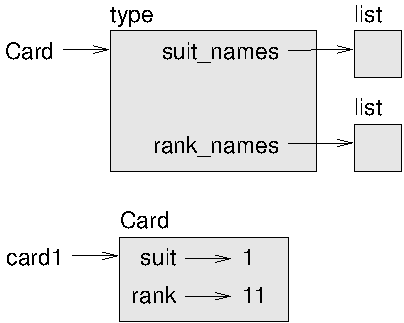
\includegraphics[scale=0.8]{figs/card1.pdf}}
\caption{แผนภาพออบเจ๊คต์}
\label{fig.card1}
\end{figure}

%Figure~\ref{fig.card1} is a diagram of the {\tt Card} class object and
%one Card instance.  {\tt Card} is a class object; its type is {\tt type}. 
%{\tt card1} is an instance of {\tt Card}, so its type is
%{\tt Card}.  To save space, I didn't draw the contents of
%\verb"suit_names" and \verb"rank_names".  

รูปที่~\ref{fig.card1} เป็นแผนภาพของคลาสออบเจ๊คต์ {\tt Card} และหนึ่งอินสแตนซ์ของ Card 
{\tt Card} เป็นคลาสออบเจ๊คต์  จึงมีชนิดเป็น {\tt type} 
ส่วน card1 เป็นอินสแตนซ์ของ {\tt Card} จึงมีชนิดเป็น {\tt Card} 
เพื่อประหยัดพื้นที่ ฉันไม่ได้วาดเนื้อหาของ \verb"suit_names" และ \verb"rank_names"
\index{state diagram}
\index{diagram!state} 
\index{object diagram} 
\index{diagram!object}
\index{แผนภาพสถานะ}
\index{แผนภาพ!สถานะ}
\index{แผนภาพออบเจ๊คต์}
\index{แผนภาพ!ออบเจ๊คต์}


%\section{Comparing cards}
\section{การเปรียบเทียบไพ่} % (Comparing cards)}
\label{comparecard}
\index{operator!relational}
\index{relational operator}
\index{ตัวดำเนินการเชิงสัมพันธ์}
\index{ตัวดำเนินการ!เชิงสัมพันธ์}

%For built-in types, there are relational operators
%({\tt <}, {\tt >}, {\tt ==}, etc.) that compare
%values and determine when one is greater than, less than, or equal to
%another.  For programmer-defined types, we can override the behavior of
%the built-in operators by providing a method named
%\verb"__lt__", which stands for ``less than''.

สำหรับชนิดที่มีอยู่แล้วในตัว มีตัวดำเนินการเชิงสัมพันธ์ ({\tt <}, {\tt >}, {\tt ==}, ฯลฯ) ที่เปรียบเทียบค่าและกำหนดว่าค่าใดค่าหนึ่งมากกว่า น้อยกว่า หรือเท่ากับค่าอื่น
สำหรับชนิดข้อมูลที่กำหนดโดยโปรแกรมเมอร์ เราสามารถแทนที่พฤติกรรมของตัวดำเนินการในตัวได้โดยการจัดเตรียมเมธอดที่ชื่อ \verb"__lt__" ซึ่งย่อมาจาก ``less than''
\index{programmer-defined type}
\index{type!programmer-defined}
\index{ชนิดข้อมูลที่ผู้เขียนโปรแกรมกำหนดเอง}
\index{ชนิดข้อมูล!ผู้เขียนโปรแกรมกำหนดเอง}

%\verb"__lt__" takes two parameters, {\tt self} and {\tt other},
%and returns {\tt True} if {\tt self} is strictly less than {\tt other}.

\verb"__lt__" รับพารามิเตอร์สองตัวคือ {\tt self} และ {\tt other} และคืนค่า {\tt True} หาก {\tt self} มีค่าน้อยกว่า {\tt other} อย่างแน่นอน

\index{override}
\index{operator overloading}
\index{แทนที่}
\index{การโอเวอร์โหลดตัวดำเนินการ}

%The correct ordering for cards is not obvious.
%For example, which
%is better, the 3 of Clubs or the 2 of Diamonds?  One has a higher
%rank, but the other has a higher suit.  In order to compare
%cards, you have to decide whether rank or suit is more important.

ลำดับที่ถูกต้องสำหรับการ์ดไม่ชัดเจน ตัวอย่างเช่น อันไหนดีกว่าระหว่าง 3 ของดอกจิก หรือ 2 ของข้าวหลามตัด? 
ใบหนึ่งมีอันดับสูงกว่า แต่อีกใบมีชุดสูงกว่า เพื่อเปรียบเทียบไพ่ คุณต้องตัดสินใจว่าอันดับหรือชุดมีความสำคัญมากกว่า


%The answer might depend on what game you are playing, but to keep
%things simple, we'll make the arbitrary choice that suit is more
%important, so all of the Spades outrank all of the Diamonds,
%and so on.

คำตอบอาจขึ้นอยู่กับว่าคุณกำลังเล่นเกมอะไรอยู่ แต่เพื่อให้ง่ายขึ้น เราจะทำการเลือกตามอำเภอใจซึ่งชุดนั้นสำคัญกว่า ดังนั้นโพดำทั้งหมดจึงมีอันดับเหนือกว่าข้าวหลามตัดทั้งหมด และอื่นๆ

\index{cmp method@\_\_cmp\_\_ method}
\index{method!\_\_cmp\_\_}
\index{เมธอด!\_\_cmp\_\_}

%With that decided, we can write \verb"__lt__":
ด้วยการตัดสินใจนั้น เราสามารถเขียน \verb"__lt__" ดังนี้

\begin{verbatim}
# inside class Card:

    def __lt__(self, other):
        # check the suits
        if self.suit < other.suit: return True
        if self.suit > other.suit: return False

        # suits are the same... check ranks
        return self.rank < other.rank
\end{verbatim}
%
%You can write this more concisely using tuple comparison:
คุณสามารถเขียนให้กระชับยิ่งขึ้นได้โดยใช้การเปรียบเทียบทูเพิล
\index{tuple!comparison}
\index{comparison!tuple}

\begin{verbatim}
# inside class Card:

    def __lt__(self, other):
        t1 = self.suit, self.rank
        t2 = other.suit, other.rank
        return t1 < t2
\end{verbatim}
%
%As an exercise, write an \verb"__lt__" method for Time objects.  You
%can use tuple comparison, but you also might consider 
%comparing integers.
เพื่อเป็นการฝึก ให้เขียนเมธอด \verb"__lt__" สำหรับออบเจ๊คต์ Time คุณสามารถใช้การเปรียบเทียบทูเพิล แต่คุณอาจพิจารณาเปรียบเทียบจำนวนเต็มด้วย 

%\section{Decks}
\section{สำรับ}
\index{list!of objects}
\index{deck, playing cards}

%Now that we have Cards, the next step is to define Decks.  Since a
%deck is made up of cards, it is natural for each Deck to contain a
%list of cards as an attribute.
ตอนนี้เรามีไพ่แล้ว ขั้นตอนต่อไปคือการประกาศ สำรับ (Deck) เนื่องจากสำรับประกอบด้วยไพ่ จึงเป็นเรื่องธรรมดาที่แต่ละสำรับจะมีรายการไพ่เป็นแอตทริบิวต์ 
\index{init method}
\index{method!init}

%The following is a class definition for {\tt Deck}.  The
%init method creates the attribute {\tt cards} and generates
%the standard set of fifty-two cards:
ต่อไปนี้เป็นนิยามสำหรับคลาส Deck เมธอด init สร้างแอตทริบิวต์ cards และสร้างชุดมาตรฐานของไพ่ห้าสิบสองใบ

\index{composition}
\index{loop!nested}
\index{Deck class}
\index{class!Deck}

\begin{verbatim}
class Deck:

    def __init__(self):
        self.cards = []
        for suit in range(4):
            for rank in range(1, 14):
                card = Card(suit, rank)
                self.cards.append(card)
\end{verbatim}
%
%The easiest way to populate the deck is with a nested loop.  The outer
%loop enumerates the suits from 0 to 3.  The inner loop enumerates the
%ranks from 1 to 13.  Each iteration
%creates a new Card with the current suit and rank,
%and appends it to {\tt self.cards}.
วิธีที่ง่ายที่สุดในการเติมข้อมูลสำรับคือการใช้ลูปที่ซ้อนกัน วงนอกระบุชุดจาก 0 ถึง 3 วงในระบุอันดับจาก 1 ถึง 13 การวนซ้ำแต่ละครั้งจะสร้างการ์ดใหม่ด้วยชุดและอันดับปัจจุบัน และผนวกเข้ากับ {\tt self.cards}
\index{append method}
\index{method!append}


%\section{Printing the deck}
\section{การพิมพ์สำรับ} % (Printing the deck)}
\label{printdeck}
\index{str method@\_\_str\_\_ method}
\index{method!\_\_str\_\_}

%Here is a \verb"__str__" method for {\tt Deck}:
นี่คือเมธอด \verb"__str__" สำหรับ {\tt Deck}

\begin{verbatim}
#inside class Deck:

    def __str__(self):
        res = []
        for card in self.cards:
            res.append(str(card))
        return '\n'.join(res)
\end{verbatim}
%
%This method demonstrates an efficient way to accumulate a large
%string: building a list of strings and then using the string method
%{\tt join}.  The built-in function {\tt str} invokes the
%\verb"__str__" method on each card and returns the string
%representation.

เมธอดนี้แสดงให้เห็นถึงวิธีที่มีประสิทธิภาพในการสะสมสตริงขนาดใหญ่ โดยสร้างลิสต์ของสตริงแล้วใช้เมธอด {\tt join} ของสตริง 
ฟังก์ชันในตัว {\tt str} เรียกใช้เมธอด \verb"__str__" บนไพ่แต่ละใบและส่งกลับการแสดงผลสตริง 
\index{accumulator!string} 
\index{string!accumulator}
\index{join method} 
\index{method!join} 
\index{newline}

%Since we invoke {\tt join} on a newline character, the cards
%are separated by newlines.  Here's what the result looks like:
เนื่องจากเราเรียก {\tt join} บนอักขระขึ้นบรรทัดใหม่ การ์ดแต่ละใบจะถูกคั่นด้วยการขึ้นบรรทัดใหม่

\begin{verbatim}
>>> deck = Deck()
>>> print(deck)
Ace of Clubs
2 of Clubs
3 of Clubs
...
10 of Spades
Jack of Spades
Queen of Spades
King of Spades
\end{verbatim}
%
%Even though the result appears on 52 lines, it is
%one long string that contains newlines.
แม้ว่าผลลัพธ์จะปรากฏใน 52 บรรทัด แต่เป็นเพียงหนึ่งสตริงยาวที่มีการขึ้นบรรทัดใหม่แทรกอยู่

%\section{Add, remove, shuffle and sort}
\section{เพิ่ม ลบ สับเปลี่ยน และจัดเรียง} % (Add, remove, shuffle and sort)}

%To deal cards, we would like a method that
%removes a card from the deck and returns it.
%The list method {\tt pop} provides a convenient way to do that:
ในการแจกไพ่ เราต้องการวิธีที่จะนำไพ่ออกจากสำรับและส่งคืนค่านั้น เมธอด {\tt pop} ของลิสต์เป็นวิธีที่สะดวกในการทำเช่นนั้น
\index{pop method}
\index{method!pop}

\begin{verbatim}
#inside class Deck:

    def pop_card(self):
        return self.cards.pop()
\end{verbatim}
%
%Since {\tt pop} removes the {\em last} card in the list, we are
%dealing from the bottom of the deck.
เนื่องจาก {\tt pop} ดึงเอาไพ่{\em ใบสุดท้าย}ในลิสต์ออก เราจึงแจกไพ่จากด้านล่างของสำรับ
\index{append method}
\index{method!append}

%To add a card, we can use the list method {\tt append}:
ในการเพิ่มการ์ด เราสามารถใช้เมธอด append ของ list

\begin{verbatim}
#inside class Deck:

    def add_card(self, card):
        self.cards.append(card)
\end{verbatim}
%
%A method like this that uses another method without doing
%much work is sometimes called a {\bf veneer}.  The metaphor
%comes from woodworking, where a veneer is a thin
%layer of good quality wood glued to the surface of a cheaper piece of
%wood to improve the appearance.

วิธีการแบบนี้ที่ใช้เมธอดอื่นโดยไม่ต้องทำอะไรมาก บางครั้งเรียกว่า {\bf วีเนียร์ (veneer)} คำอุปมานี้มาจากงานไม้ 
โดยที่แผ่นไม้อัดเป็นชั้นไม้คุณภาพดีบางๆ ที่ติดกาวบนพื้นผิวของแผ่นไม้ที่ราคาถูกกว่าเพื่อปรับปรุงรูปลักษณ์

\index{veneer}

%In this case \verb"add_card" is a ``thin'' method that expresses
%a list operation in terms appropriate for decks.  It
%improves the appearance, or interface, of the
%implementation.

ในกรณีนี้ \verb"add_card" เป็น เมธอด ``บาง'' ที่ใช้การดำเนินการของลิสต์ในแง่ที่เหมาะสมสำหรับสำรับ เพื่อปรับปรุงลักษณะที่ปรากฏหรือส่วนต่อประสานของการใช้งาน

%As another example, we can write a Deck method named {\tt shuffle}
%using the function {\tt shuffle} from the {\tt random} module:
อีกตัวอย่างหนึ่ง เราสามารถเขียนเมธอดของ Deck ชื่อ {\tt shuffle} โดยใช้ฟังก์ชัน {\tt shuffle} จากโมดูล {\tt random}:

\index{random module}
\index{module!random}
\index{shuffle function}
\index{function!shuffle}

\begin{verbatim}
# inside class Deck:
            
    def shuffle(self):
        random.shuffle(self.cards)
\end{verbatim}
%
%Don't forget to import {\tt random}.
อย่าลืมนำเข้า {\tt random}

%As an exercise, write a Deck method named {\tt sort} that uses the
%list method {\tt sort} to sort the cards in a {\tt Deck}.  {\tt sort}
%uses the \verb"__lt__" method we defined to determine the order.

เพื่อเป็นการฝึกหัด ให้เขียนเมธอดของ Deck ชื่อ {\tt sort} ซึ่งใช้เมธอด {\tt sort} ของลิสต์ เพื่อจัดเรียงไพ่ในสำรับ  
โดยให้ sort ใช้เมธอด \verb"__lt__" ที่เราได้นิยามไว้เพื่อกำหนดลำดับก่อนหลัง
\index{sort method} \index{method!sort}



%\section{Inheritance}
\section{การสืบทอด} % (Inheritance)}
\index{inheritance}
\index{object-oriented programming}

%Inheritance is the ability to define a new class that is a modified
%version of an existing class.  As an example, let's say we want a
%class to represent a ``hand'', that is, the cards held by one player.
%A hand is similar to a deck: both are made up of a collection of
%cards, and both require operations like adding and removing cards.

การสืบทอดคือความสามารถในการสร้างคลาสใหม่ที่เป็นรุ่นที่แก้ไขของคลาสที่มีอยู่ ตัวอย่างเช่น สมมติว่าเราต้องการให้คลาสเป็นตัวแทนของ ``hand'' 
ซึ่งเป็นไพ่ที่ผู้เล่นคนหนึ่งถือไว้ในมือ hand คล้ายกันกับ Deck คือทั้งสองประกอบด้วยชุดไพ่ และทั้งคู่ต้องมีการดำเนินการเช่นการเพิ่มและนำไพ่ออก


%A hand is also different from a deck; there are operations we want for
%hands that don't make sense for a deck.  For example, in poker we
%might compare two hands to see which one wins.  In bridge, we might
%compute a score for a hand in order to make a bid.

มือ ก็แตกต่างจากสำรับ คือมีการดำเนินการที่เราต้องการสำหรับมือ ที่ไม่สมเหตุสมผลสำหรับสำรับ 
ตัวอย่างเช่น ในโป๊กเกอร์ เราอาจเปรียบเทียบสองมือเพื่อดูว่าใครชนะ ในบริดจ์เราอาจคำนวณคะแนนสำหรับมือเพื่อบิด


%This relationship between classes---similar, but different---lends
%itself to inheritance.
%To define a new class that inherits from an existing class,
%you put the name of the existing class in parentheses:

ความสัมพันธ์ระหว่างคลาสนี้คล้ายกันแต่ต่างกันนำไปสู่การสืบทอด ในการประกาศคลาสใหม่ที่สืบทอดมาจากคลาสที่มีอยู่ คุณใส่ชื่อของคลาสที่มีอยู่ในวงเล็บ:

\index{parentheses!parent class in}
\index{parent class}
\index{class!parent}
\index{Hand class}
\index{class!Hand}

\begin{verbatim}
class Hand(Deck):
    """Represents a hand of playing cards."""
\end{verbatim}
%
%This definition indicates that {\tt Hand} inherits from {\tt Deck};
%that means we can use methods like \verb"pop_card" and \verb"add_card"
%for Hands as well as Decks.

ในการประกาศนี้บ่งชี้ว่า {\tt Hand} สืบทอดมาจาก {\tt Deck} นั่นหมายความว่าเราสามารถใช้วิธีต่างๆ 
เช่น \verb"pop_card" และ \verb"add_card" สำหรับ Hands เช่นเดียวกับ Decks

%When a new class inherits from an existing one, the existing
%one is called the {\bf parent} and the new class is
%called the {\bf child}.
เมื่อคลาสใหม่สืบทอดมาจากคลาสที่มีอยู่ คลาสที่มีอยู่จะเรียกว่า {\bf พาเรนต์ (parent)} และคลาสใหม่จะถูกเรียกว่า {\bf ลูก (child)}

\index{parent class}
\index{child class}
\index{class!child}

%In this example, {\tt Hand} inherits \verb"__init__" from {\tt Deck},
%but it doesn't really do what we want: instead of populating the hand
%with 52 new cards, the init method for Hands should initialize {\tt   cards} with an empty list.  

ในตัวอย่างนี้ {\tt Hand} สืบทอด \verb"__init__" จาก {\tt Deck} แต่มันไม่ได้ทำในสิ่งที่เราต้องการ 
แทนที่จะเติมไพ่ใหม่ 52 ใบบนมือ เมธอด init สำหรับ Hands ควรเริ่มต้น {\tt cards} ด้วยรายการที่ว่างเปล่า
\index{override} 
\index{init method}
\index{method!init}

%If we provide an init method in the {\tt Hand} class, it overrides the
%one in the {\tt Deck} class:
ถ้าเราจัดเตรียมเมธอด init ในคลาส {\tt Hand} มันจะไปแทนที่เมธอดในคลาส {\tt Deck}

\begin{verbatim}
# inside class Hand:

    def __init__(self, label=''):
        self.cards = []
        self.label = label
\end{verbatim}
%
%When you create a Hand, Python invokes this init method, not the
%one in {\tt Deck}.
เมื่อคุณสร้างอินสแตนซ์ของ Hand ไพธอนจะเรียกใช้เมธอด init นี้ ไม่ใช่เมธอดใน {\tt Deck}

\begin{verbatim}
>>> hand = Hand('new hand')
>>> hand.cards
[]
>>> hand.label
'new hand'
\end{verbatim}
%
%The other methods are inherited from {\tt Deck}, so we can use
%\verb"pop_card" and \verb"add_card" to deal a card:
เมธอดอื่นๆ นั้นสืบทอดมาจาก {\tt Deck} ดังนั้นเราจึงสามารถใช้ \verb"pop_card" และ \verb"add_card" เพื่อจัดการไพ่ได้

\begin{verbatim}
>>> deck = Deck()
>>> card = deck.pop_card()
>>> hand.add_card(card)
>>> print(hand)
King of Spades
\end{verbatim}
%
%A natural next step is to encapsulate this code in a method
%called \verb"move_cards":
ขั้นตอนต่อไปที่เป็นธรรมชาติคือการห่อหุ้มโค้ดนี้ด้วยวิธีการที่เรียกว่า \verb"move_cards"
\index{encapsulation}

\begin{verbatim}
#inside class Deck:

    def move_cards(self, hand, num):
        for i in range(num):
            hand.add_card(self.pop_card())
\end{verbatim}
%
%\verb"move_cards" takes two arguments, a Hand object and the number of
%cards to deal.  It modifies both {\tt self} and {\tt hand}, and
%returns {\tt None}.

\verb"move_cards" รับสองอาร์กิวเมนต์ ออบเจ๊คต์ Hand และจำนวนไพ่ที่จะจัดการ มันปรับเปลี่ยนทั้ง {\tt self} และ {\tt hand} แล้วส่งกลับ {\tt None}


%In some games, cards are moved from one hand to another,
%or from a hand back to the deck.  You can use \verb"move_cards"
%for any of these operations: {\tt self} can be either a Deck
%or a Hand, and {\tt hand}, despite the name, can also be a {\tt Deck}.

ในบางเกม ไพ่จะถูกย้ายจากมือหนึ่งไปอีกมือหนึ่ง หรือจากมือกลับไปที่สำรับ คุณสามารถใช้ \verb"move_cards" 
สำหรับการดำเนินการใด ๆ เหล่านี้ เพราะ {\tt self} สามารถเป็น Deck หรือ Hand ก็ได้  ไม่ว่าจะเป็นชนิดใด ต่างก็สามารถใช้ในนาม Deck ได้


%Inheritance is a useful feature.  Some programs that would be
%repetitive without inheritance can be written more elegantly
%with it.  Inheritance can facilitate code reuse, since you can
%customize the behavior of parent classes without having to modify
%them.  In some cases, the inheritance structure reflects the natural
%structure of the problem, which makes the design easier to
%understand.

การสืบทอดเป็นคุณลักษณะที่มีประโยชน์ บางโปรแกรมที่ทำซ้ำๆ โดยไม่มีการสืบทอดจะสามารถเขียนได้อย่างสวยงามยิ่งขึ้นด้วยการสืบทอด  การสืบทอดสามารถอำนวยความสะดวก
ในการนำรหัสมาใช้ซ้ำ เนื่องจากคุณสามารถปรับแต่งพฤติกรรมของคลาสพาเรนต์โดยไม่ต้องแก้ไขพวกมัน ในบางกรณีโครงสร้างการสืบทอดจะสะท้อนถึงโครงสร้างตามธรรมชาติของปัญหา 
ซึ่งทำให้สามารถเข้าใจการออกแบบได้ง่ายขึ้น


%On the other hand, inheritance can make programs difficult to read.
%When a method is invoked, it is sometimes not clear where to find its
%definition.  The relevant code may be spread across several modules.
%Also, many of the things that can be done using inheritance can be
%done as well or better without it.

ในทางกลับกัน การสืบทอดอาจทำให้โปรแกรมอ่านยาก เมื่อมีการเรียกใช้เมธอด บางครั้งก็ไม่ชัดเจนว่าจะหานิยามได้จากที่ใด 
รหัสที่เกี่ยวข้องอาจกระจายไปทั่วหลายโมดูล นอกจากนี้ หลายๆ อย่างที่สามารถทำได้โดยใช้การสืบทอด ก็สามารถทำได้เช่นกันหรือทำได้ดีกว่าโดยไม่ใช้การสืบทอด


%\section{Class diagrams}
\section{แผนภาพคลาส } %(Class diagrams)}
\label{class.diagram}

%So far we have seen stack diagrams, which show the state of
%a program, and object diagrams, which show the attributes
%of an object and their values.  These diagrams represent a snapshot
%in the execution of a program, so they change as the program
%runs.

จนถึงตอนนี้ เราได้เห็นแผนภาพสแต็ก ซึ่งแสดงสถานะของโปรแกรม และแผนภาพของออบเจ๊คต์ ซึ่งแสดงแอตทริบิวต์ของออบเจ๊คต์และค่าของมัน 
แผนภาพเหล่านี้แสดงสแนปชอตในการทำงานของโปรแกรม ดังนั้นจจึงมีการเปลี่ยนแปลงขณะโปรแกรมทำงาน


%They are also highly detailed; for some purposes, too
%detailed.  A class diagram is a more abstract representation
%of the structure of a program.  Instead of showing individual
%objects, it shows classes and the relationships between them.

นอกจากนี้ยังมีรายละเอียดสูงเพื่อจุดประสงค์บางอย่างที่ละเอียดเกินไป 
แผนภาพคลาสเป็นตัวแทนของโครงสร้างของโปรแกรมที่เป็นนามธรรมมากขึ้น 
แทนที่จะแสดงแต่ละออบเจ๊คต์ จะแสดงคลาสและความสัมพันธ์ระหว่างออบเจ๊คต์


%There are several kinds of relationship between classes:
มีความสัมพันธ์ระหว่างคลาสหลายประเภท

\begin{itemize}

%\item Objects in one class might contain references to objects
%in another class.  For example, each Rectangle contains a reference
%to a Point, and each Deck contains references to many Cards.
%This kind of relationship is called {\bf HAS-A}, as in, ``a Rectangle
%has a Point.''

\item ออบเจ๊คต์ในคลาสหนึ่งอาจมีการอ้างอิงถึงออบเจ๊คต์ในอีกคลาสหนึ่ง ตัวอย่างเช่น สี่เหลี่ยมผืนผ้าแต่ละอันมีการอ้างอิงไปยังจุด 
และแต่ละสำรับมีการอ้างอิงถึงไพ่หลายใบ ความสัมพันธ์แบบนี้เรียกว่า {\bf มี (HAS-A)} เช่น ``สี่เหลี่ยมผืนผ้ามีจุด''

%\item One class might inherit from another.  This relationship
%is called {\bf IS-A}, as in, ``a Hand is a kind of a Deck.''

\item คลาสหนึ่งอาจสืบทอดมาจากอีกคลาสหนึ่ง ความสัมพันธ์นี้เรียกว่า {\bf เป็น (IS-A)} เช่น ``มือเป็นสำรับชนิดหนึ่ง''

%\item One class might depend on another in the sense that objects
%in one class take objects in the second class as parameters, or
%use objects in the second class as part of a computation.  This
%kind of relationship is called a {\bf dependency}.

\item คลาสหนึ่งอาจขึ้นอยู่กับอีกคลาสหนึ่งในแง่ที่ว่าอ็อบเจ๊คต์ในคลาสหนึ่งใช้อ็อบเจ๊คต์ในคลาสที่สองเป็นพารามิเตอร์ 
หรือใช้อ็อบเจ๊คต์ในคลาสที่สองเป็นส่วนหนึ่งของการคำนวณ ความสัมพันธ์แบบนี้เรียกว่า {\bf การขึ้นต่อกัน (dependency)}

\end{itemize}
\index{IS-A relationship}
\index{HAS-A relationship}
\index{class diagram}
\index{diagram!class}

%A {\bf class diagram} is a graphical representation of these
%relationships.  For example, Figure~\ref{fig.class1} shows the
%relationships between {\tt Card}, {\tt Deck} and {\tt Hand}.

{\bf แผนภาพคลาส}เป็นการแสดงกราฟิกของความสัมพันธ์เหล่านี้ ตัวอย่างเช่น รูปที่~\ref{fig.class1} 
แสดงความสัมพันธ์ระหว่าง {\tt Card}, {\tt Deck} และ {\tt Hand}

\begin{figure}
\centerline
{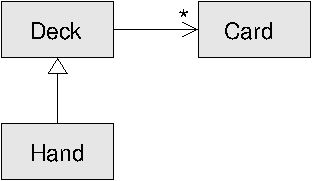
\includegraphics[scale=0.8]{figs/class1.pdf}}
\caption{แผนภาพคลาส}
\label{fig.class1}
\end{figure}

%The arrow with a hollow triangle head represents an IS-A
%relationship; in this case it indicates that Hand inherits
%from Deck.

ลูกศรที่มีหัวสามเหลี่ยมกลวงแสดงถึงความสัมพันธ์แบบ เป็น (IS-A) ในกรณีนี้แสดงว่ามือนั้นสืบทอดมาจากสำรับ

% The standard arrow head represents a HAS-A
% relationship; in this case a Deck has references to Card
% objects.

หัวลูกศรมาตรฐานแสดงถึงความสัมพันธ์แบบ มี (HAS-A) ในกรณีนี้เด็คมีการอ้างอิงถึงอ็อบเจ็คต์ของการ์ด
\index{multiplicity (in class diagram)}

% The star ({\tt *}) near the arrow head is a 
% {\bf multiplicity}; it indicates how many Cards a Deck has.
% A multiplicity can be a simple number, like {\tt 52}, a range,
% like {\tt 5..7} or a star, which indicates that a Deck can
% have any number of Cards.

ดาว ({\tt *}) ใกล้หัวลูกศรเป็น{\bf ความหลายหลาก (multiplicity)} มันบ่งบอกว่าสำรับมีการ์ดกี่ใบ 
ความหลายหลากอาจเป็นตัวเลขธรรมดา เช่น {\tt 52} หรือเป็นช่วง เช่น {\tt 5..7} หรือเป็นดาว ซึ่งบ่งชี้ว่าสำรับสามารถมีการ์ดจำนวนเท่าใดก็ได้

% There are no dependencies in this diagram.  They would normally
% be shown with a dashed arrow.  Or if there are a lot of
% dependencies, they are sometimes omitted.

ไม่มีการพึ่งพาในแผนภาพนี้ โดยปกติจะแสดงด้วยลูกศรประ หรือหากมีการพึ่งพากันมากบางครั้งก็ละเว้น 

% A more detailed diagram might show that a Deck actually
% contains a {\em list} of Cards, but built-in types
% like list and dict are usually not included in class diagrams.

แผนภาพที่มีรายละเอียดมากขึ้นอาจแสดงว่าสำรับมี{\em ลิสต์}ของไพ่ แต่ชนิดข้อมูลภายใน เช่น ลิสต์และดิกต์ มักจะไม่รวมอยู่ในแผนภาพคลาส

%\section{Debugging}
\section{การดีบัก}
\index{debugging}
\index{การดีบัก}

% Inheritance can make debugging difficult because when you invoke a
% method on an object, it might be hard to figure out which method will
% be invoked.  
การสืบทอดอาจทำให้การดีบักทำได้ยาก เนื่องจากเมื่อคุณเรียกใช้เมธอดบนออบเจ๊คต์ อาจเป็นเรื่องยากที่จะทราบว่าเมธอดใดจะถูกเรียกใช้ 
\index{inheritance}

% Suppose you are writing a function that works with Hand objects.
% You would like it to work with all kinds of Hands, like
% PokerHands, BridgeHands, etc.  If you invoke a method like
% {\tt shuffle}, you might get the one defined in {\tt Deck},
% but if any of the subclasses override this method, you'll
% get that version instead.  This behavior is usually a good
% thing, but it can be confusing.

สมมติว่าคุณกำลังเขียนฟังก์ชันที่ทำงานกับอ๊อบเจ็คต์ Hand คุณต้องการให้มันทำงานกับทุกประเภทของ Hand 
เช่น PokerHands, BridgeHands เป็นต้น หากคุณเรียกใช้เมธอดเช่น {\tt shuffle} 
คุณอาจได้รับเมธอดที่กำหนดไว้ใน {\tt Deck} แต่ถ้าคลาสย่อยใดแทนที่เมธอดนี้ คุณจะได้รับรุ่นนั้นแทน พฤติกรรมนี้มักจะเป็นสิ่งที่ดี แต่อาจทำให้สับสนได้


% Any time you are unsure about the flow of execution through your
% program, the simplest solution is to add print statements at the
% beginning of the relevant methods.  If {\tt Deck.shuffle} prints a
% message that says something like {\tt Running Deck.shuffle}, then as
% the program runs it traces the flow of execution.

ทุกครั้งที่คุณไม่แน่ใจเกี่ยวกับโฟลว์ของการทำงานในโปรแกรมของคุณ วิธีที่ง่ายที่สุดคือการเพิ่มคำสั่งการพิมพ์ที่จุดเริ่มต้นของเมธอดที่เกี่ยวข้อง 
ถ้าเป็น {\tt Deck.shuffle} ก็พิมพ์ข้อความที่เขียนว่า {\tt Running Deck.shuffle} เมื่อโปรแกรมรันจะแสดงร่องรอยโฟลว์ของการทำงาน
\index{flow of execution}


% As an alternative, you could use this function, which takes an
% object and a method name (as a string) and returns the class that
% provides the definition of the method:

อีกทางเลือกหนึ่ง คุณสามารถใช้ฟังก์ชันต่อไปนี้ ซึ่งรับชื่อออบเจ๊คต์และเมธอด (เป็นสตริง) แล้วส่งคืนคลาสที่มีนิยามของเมธอด

\begin{verbatim}
def find_defining_class(obj, meth_name):
    for ty in type(obj).mro():
        if meth_name in ty.__dict__:
            return ty
\end{verbatim}
%
%Here's an example:
นี่เป็นตัวอย่างการใช้

\begin{verbatim}
>>> hand = Hand()
>>> find_defining_class(hand, 'shuffle')
<class 'Card.Deck'>
\end{verbatim}
%
%So the {\tt shuffle} method for this Hand is the one in {\tt Deck}.

ดังนั้นเมธอด {\tt shuffle} สำหรับ  Hand นี้เป็นเมธอดหนึ่งใน {\tt Deck}

\index{mro method}
\index{method!mro}
\index{method resolution order}

% \verb"find_defining_class" uses the {\tt mro} method to get the list
% of class objects (types) that will be searched for methods.  ``MRO''
% stands for ``method resolution order'', which is the sequence of
% classes Python searches to ``resolve'' a method name.

\verb"find_defining_class" ใช้เมธอด {\tt mro} เพื่อรับรายการคลาสออบเจ๊คต์ (ชนิดข้อมูล) ที่จะค้นหาเมธอด 
``MRO'' ย่อมาจาก ``ลำดับการแก้ไขเมธอด (method resolution order)'' ซึ่งเป็นลำดับของคลาสที่ไพธอนค้นหาเพื่อ ``ตัดสินใจ (resolve)'' ชื่อเมธอด


% Here's a design suggestion: when you override a method,
% the interface of the new method should be the same as the old.  It
% should take the same parameters, return the same type, and obey the
% same preconditions and postconditions.  If you follow this rule, you
% will find that any function designed to work with an instance of a
% parent class, like a Deck, will also work with instances of child
% classes like a Hand and PokerHand.

นี่คือคำแนะนำการออกแบบ: เมื่อคุณลบล้างเมธอด อินเทอร์เฟซของเมธอดใหม่ควรเหมือนกับเมธอดเก่า ควรใช้พารามิเตอร์เดียวกัน ส่งคืนประเภทเดียวกัน และปฏิบัติตามเงื่อนไขเบื้องต้นและเงื่อนไขภายหลังเดียวกัน 
หากคุณทำตามกฎนี้ คุณจะพบว่าฟังก์ชันใดๆ ที่ออกแบบมาเพื่อทำงานกับอินสแตนซ์ของคลาสหลัก เช่น เด็ค จะทำงานกับอินสแตนซ์ของคลาสย่อย เช่น Hand และ PokerHand

\index{override}
\index{interface}
\index{precondition}
\index{postcondition}

% If you violate this rule, which is called the ``Liskov substitution
% principle'', your code will collapse like (sorry) a house of cards.

หากคุณละเมิดกฎนี้ ซึ่งเรียกว่า ``หลักการทดแทนของ Liskov'' รหัสโปรแกรมของคุณจะพังเหมือน (น่าสลดใจ) บ้านไพ่
\index{Liskov substitution principle}


%\section{Data encapsulation}
\section{การห่อหุ้มข้อมูล} % (Data encapsulation)}

% The previous chapters demonstrate a development plan we might call
% ``object-oriented design''.  We identified objects we needed---like
% {\tt Point}, {\tt Rectangle} and {\tt Time}---and defined classes to
% represent them.  In each case there is an obvious correspondence
% between the object and some entity in the real world (or at least a
% mathematical world).  
บทก่อนหน้านี้แสดงให้เห็นถึงแผนการพัฒนาที่เราอาจเรียกว่า ``การออกแบบเชิงวัตถุ'' เราจำแนกออบเจ๊คต์ที่เราต้องการ  เช่น {\tt Point}, {\tt Rectangle} และ {\tt Time}
และกำหนดคลาสเพื่อเป็นตัวแทนของพวกมัน ในแต่ละกรณี มีความสอดคล้องกันอย่างชัดเจนระหว่างวัตถุและเอนทิตีบางอย่างในโลกแห่งความเป็นจริง (หรืออย่างน้อยก็โลกทางคณิตศาสตร์)

\index{development plan!data encapsulation}

But sometimes it is less obvious what objects you need
and how they should interact.  In that case you need a different
development plan.  In the same way that we discovered function
interfaces by encapsulation and generalization, we can discover
class interfaces by {\bf data encapsulation}.

แต่บางครั้งก็ไม่ชัดเจนว่าคุณต้องการอ๊อบเจ็คต์อะไรและควรโต้ตอบอย่างไร ในกรณีนั้นคุณต้องมีแผนการพัฒนาที่แตกต่างออกไป 
ในลักษณะเดียวกับที่เราค้นพบอินเทอร์เฟซของฟังก์ชันโดยการห่อหุ้มและการวางนัยทั่วไป เราสามารถค้นพบอินเทอร์เฟซของคลาสได้โดย{\bf การห่อหุ้มข้อมูล (data encapsulation)}
\index{data encapsulation}

% Markov analysis, from Section~\ref{markov}, provides a good example.
% If you download my code from \url{http://thinkpython2.com/code/markov.py},
% you'll see that it uses two global variables---\verb"suffix_map" and
% \verb"prefix"---that are read and written from several functions.

การวิเคราะห์ Markov จากส่วนที่~\ref{markov} เป็นตัวอย่างที่ดี หากคุณดาวน์โหลดโค้ดของฉันจาก \url{http://thinkpython2.com/code/markov.py} 
คุณจะเห็นว่ามันใช้ตัวแปรส่วนกลางสองตัว \verb"suffix_map" และ \verb"prefix" ที่ถูกอ่านและเขียนจากหลายฟังก์ชัน


\begin{verbatim}
suffix_map = {}        
prefix = ()            
\end{verbatim}

% Because these variables are global, we can only run one analysis at a
% time.  If we read two texts, their prefixes and suffixes would be
% added to the same data structures (which makes for some interesting
% generated text).

เนื่องจากตัวแปรเหล่านี้เป็นตัวแปรส่วนกลาง เราจึงสามารถเรียกใช้การวิเคราะห์ได้ครั้งละหนึ่งรายการเท่านั้น 
ถ้าเราอ่านสองข้อความ คำนำหน้าและส่วนต่อท้ายจะถูกเพิ่มในโครงสร้างข้อมูลเดียวกัน (ซึ่งทำให้บางข้อความที่สร้างขึ้นน่าสนใจ)

% To run multiple analyses, and keep them separate, we can encapsulate
% the state of each analysis in an object.
% Here's what that looks like:

เพื่อที่จะเรียกใช้การวิเคราะห์หลายรายการและวิเคราะห์แยกกัน เราสามารถห่อหุ้มสถานะของการวิเคราะห์แต่ละรายการในออบเจ็กต์ได้ มีหน้าตาประมาณนี้

\begin{verbatim}
class Markov:

    def __init__(self):
        self.suffix_map = {}
        self.prefix = ()    
\end{verbatim}

% Next, we transform the functions into methods.  For example,
% here's \verb"process_word":

ถัดไปเราแปลงฟังก์ชันเป็นเมธอด ตัวอย่างเช่น \verb"process_word" ดังต่อไปนี้

\begin{verbatim}
    def process_word(self, word, order=2):
        if len(self.prefix) < order:
            self.prefix += (word,)
            return

        try:
            self.suffix_map[self.prefix].append(word)
        except KeyError:
            # if there is no entry for this prefix, make one
            self.suffix_map[self.prefix] = [word]

        self.prefix = shift(self.prefix, word)        
\end{verbatim}

% Transforming a program like this---changing the design without
% changing the behavior---is another example of refactoring
% (see Section~\ref{refactoring}).

การแปลงโปรแกรมในลักษณะนี้ คือการเปลี่ยนการออกแบบโดยไม่เปลี่ยนลักษณะการทำงาน เป็นอีกตัวอย่างหนึ่งของการปรับโครงสร้างใหม่ (ดูส่วนที่~\ref{refactoring})

\index{refactoring}

This example suggests a development plan for designing objects and
methods:

ตัวอย่างนี้แนะนำแผนการพัฒนาสำหรับการออกแบบออบเจ๊คต์และเมธอด

\begin{enumerate}

% \item Start by writing functions that read and write global
% variables (when necessary).
\item เริ่มต้นด้วยการเขียนฟังก์ชันที่อ่านและเขียนตัวแปรส่วนกลาง (เมื่อจำเป็น)

% \item Once you get the program working, look for associations
% between global variables and the functions that use them.
\item เมื่อคุณทำให้โปรแกรมทำงานได้ ให้มองหาความสัมพันธ์ระหว่างตัวแปรส่วนกลางและฟังก์ชันที่ใช้ตัวแปรเหล่านั้น

% \item Encapsulate related variables as attributes of an object.
\item ห่อหุ้มตัวแปรที่เกี่ยวข้องเป็นแอตทริบิวต์ของออบเจ๊คต์

% \item Transform the associated functions into methods of the new
% class.
\item แปลงฟังก์ชันที่เกี่ยวข้องเป็นเมธอดของคลาสใหม่

\end{enumerate}

% As an exercise, download my Markov code from
% \url{http://thinkpython2.com/code/markov.py}, and follow the steps
% described above to encapsulate the global variables as attributes of a
% new class called {\tt Markov}.  Solution:
% \url{http://thinkpython2.com/code/Markov.py} (note the capital M).

เพื่อเป็นการฝึกหัด ให้ดาวน์โหลดโค้ด Markov ของฉันจาก \url{http://thinkpython2.com/code/markov.py} 
และทำตามขั้นตอนที่อธิบายไว้ข้างต้นเพื่อห่อหุ้มตัวแปรส่วนกลางเป็นแอตทริบิวต์ของคลาสใหม่ที่เรียกว่า {\tt Markov} 
เฉลย: \url{http://thinkpython2.com/code/Markov.py} (สังเกตตัวพิมพ์ใหญ่ M)


%\section{Glossary}
\section{อภิธานศัพท์}

\begin{description}

% \item [encode:]  To represent one set of values using another
% set of values by constructing a mapping between them.

\item[เข้ารหัส (encode):] การแทนค่าชุดหนึ่งด้วยชุดค่าอื่นโดยสร้างการแปลงระหว่างค่าเหล่านี้
\index{encode}

% \item [class attribute:] An attribute associated with a class
% object.  Class attributes are defined inside
% a class definition but outside any method.

\item[คลาสแอตทริบิวต์ (class attribute):] แอตทริบิวต์ที่เกี่ยวข้องกับคลาสออบเจ๊คต์ ซึ่งถูกประกาศไว้ภายในนิยามคลาส แต่อยู่นอกเมธอดใดๆ
\index{class attribute}
\index{attribute!class}

% \item [instance attribute:] An attribute associated with an
% instance of a class.

\item[อินสแตนซ์แอตทริบิวต์ (instance attribute):] แอตทริบิวต์ที่เกี่ยวข้องกับอินสแตนซ์ของคลาส
\index{instance attribute}
\index{attribute!instance}

% \item [veneer:] A method or function that provides a different
% interface to another function without doing much computation.

\item[วีเนียร์ (veneer):] เมธอดหรือฟังก์ชันที่ให้อินเทอร์เฟซที่แตกต่างกันไปยังฟังก์ชันอื่นโดยไม่ต้องคำนวณมาก
\index{veneer}

% \item [inheritance:] The ability to define a new class that is a
% modified version of a previously defined class.

\item[การสืบทอด(inheritance):] ความสามารถในการนิยามคลาสใหม่ที่เป็นรุ่นที่แก้ไขของคลาสที่นิยามไว้ก่อนหน้านี้ 
\index{inheritance}

% \item [parent class:] The class from which a child class inherits.

\item[คลาสพาเรนต์ (parent class):] คลาสที่คลาสลูกสืบทอดมา
\index{parent class}

% \item [child class:] A new class created by inheriting from an
% existing class; also called a ``subclass''.

\item[คลาสลูก (child class):] คลาสใหม่ที่สร้างขึ้นโดยสืบทอดจากคลาสที่มีอยู่ เรียกอีกอย่างว่า ``คลาสย่อย''
\index{child class}
\index{class!child}

% \item [IS-A relationship:] A relationship between a child class
% and its parent class.

\item[ ความสัมพันธ์แบบเป็น (IS-A relationship):] ความสัมพันธ์ระหว่างคลาสลูกกับคลาสพาเรนต์
\index{IS-A relationship}

% \item [HAS-A relationship:] A relationship between two classes
% where instances of one class contain references to instances of
% the other.

\item[ความสัมพันธ์แบบมี (HAS-A relationship):]  ความสัมพันธ์ระหว่างสองคลาสโดยที่อินสแตนซ์ของคลาสหนึ่งมีการอ้างอิงถึงอินสแตนซ์ของอีกคลาสหนึ่ง
\index{HAS-A relationship}

% \item [dependency:] A relationship between two classes
% where instances of one class use instances of the other class,
% but do not store them as attributes.

\item[การขึ้นต่อกัน (dependency):] ความสัมพันธ์ระหว่างสองคลาสโดยที่อินสแตนซ์ของคลาสหนึ่งใช้อินสแตนซ์ของคลาสอื่น แต่ไม่เก็บไว้เป็นแอตทริบิวต์
\index{HAS-A relationship}

% \item [class diagram:] A diagram that shows the classes in a program
% and the relationships between them.

\item[แผนภาพคลาส (class diagram):] แผนภาพที่แสดงคลาสในโปรแกรมและความสัมพันธ์ระหว่างพวกเขา
\index{class diagram}
\index{diagram!class}

% \item [multiplicity:] A notation in a class diagram that shows, for
% a HAS-A relationship, how many references there are to instances
% of another class.

\item[ความหลายหลาก (multiplicity):] สัญกรณ์ในแผนภาพคลาสที่แสดงสำหรับความสัมพันธ์แบบมี ว่ามีการอ้างอิงถึงอินสแตนซ์ของคลาสอื่นกี่รายการ
\index{multiplicity (in class diagram)}

% \item [data encapsulation:]  A program development plan that
% involves a prototype using global variables and a final version
% that makes the global variables into instance attributes. 

\item[การห่อหุ้มข้อมูล (data encapsulation):] แผนการพัฒนาโปรแกรมที่เกี่ยวข้องกับต้นแบบโดยใช้ตัวแปรส่วนกลางและเวอร์ชันสุดท้ายที่ทำให้ตัวแปรส่วนกลางเป็นแอตทริบิวต์ของอินสแตนซ์
\index{data encapsulation}
\index{development plan!data encapsulation}

\end{description}


%\section{Exercises}
\section{แบบฝึกหัด}


\begin{exercise}
% For the following program, draw a UML class diagram that shows
% these classes and the relationships among them.

สำหรับโปรแกรมต่อไปนี้ ให้วาดแผนภาพคลาส UML ที่แสดงคลาสเหล่านี้และความสัมพันธ์ระหว่างคลาสเหล่านี้

\begin{verbatim}
class PingPongParent:
    pass

class Ping(PingPongParent):
    def __init__(self, pong):
        self.pong = pong


class Pong(PingPongParent):
    def __init__(self, pings=None):
        if pings is None:
            self.pings = []
        else:
            self.pings = pings

    def add_ping(self, ping):
        self.pings.append(ping)

pong = Pong()
ping = Ping(pong)
pong.add_ping(ping)
\end{verbatim}


\end{exercise}



\begin{exercise}
% Write a Deck method called \verb"deal_hands" that
% takes two parameters, the number of hands and the number of cards per
% hand.  It should create the appropriate number of Hand objects, deal
% the appropriate number of cards per hand, and return a list of Hands.

เขียนเมธอดสำหรับ Deck ที่เรียกว่า \verb"deal_hands" ซึ่งใช้พารามิเตอร์สองตัว คือ 
จำนวนมือและจำนวนไพ่ต่อมือ มันควรสร้างจำนวนของออบเจ๊คต์มือ (Hand) ที่เหมาะสม แจกไพ่ตามจำนวนที่เหมาะสมต่อมือ และส่งคืนลิสต์ของมือ

\end{exercise}


\begin{exercise}
\label{poker}

% The following are the possible hands in poker, in increasing order
% of value and decreasing order of probability:

ต่อไปนี้เป็นมือที่เป็นไปได้ในโป๊กเกอร์ โดยเรียงตามมูลค่าที่เพิ่มขึ้นและลำดับความน่าจะเป็นที่ลดลง
\index{poker}

\begin{description}

%\item[pair:] two cards with the same rank
\item[คู่ (pair):] ไพ่สองใบที่มีอันดับเดียวกัน
\vspace{-0.05in}

%\item[two pair:] two pairs of cards with the same rank
\item[สองคู่ (two pair):] ไพ่สองคู่ที่มีอันดับเดียวกัน
\vspace{-0.05in}

%\item[three of a kind:] three cards with the same rank
\item[ตอง (three of a kind):] ไพ่สามใบที่มีอันดับเดียวกัน
\vspace{-0.05in}

% \item[straight:] five cards with ranks in sequence (aces can
% be high or low, so {\tt Ace-2-3-4-5} is a straight and so is {\tt 10-Jack-Queen-King-Ace}, but {\tt Queen-King-Ace-2-3} is not.)
\item[สเตรท (straight):] ไพ่ห้าใบที่มีอันดับตามลำดับ (เอซสามารถสูงหรือต่ำได้ ดังนั้น {\tt เอซ-2-3-4-5} จึงเป็นไพ่สเตรท 
และ {\tt 10-แจ๊ค-แหม่ม-คิง-เอซ} ก็เช่นกัน แต่ {\tt แหม่ม-คิง-เอซ-2-3} ไม่ใช่.)
\vspace{-0.05in}

% \item[flush:] five cards with the same suit
\item[ฟลัช (flush):] ไพ่ห้าใบที่เป็นชุดเดียวกัน
\vspace{-0.05in}

% \item[full house:] three cards with one rank, two cards with another
\item[ฟูลเฮ้าส์ (full house):] มี 1 ตอง และ 1 คู่
\vspace{-0.05in}

% \item[four of a kind:] four cards with the same rank
\item[โฟร์การ์ด (four of a kind):] ไพ่ 4 ใบแต้มเหมือนกัน
\vspace{-0.05in}

% \item[straight flush:] five cards in sequence (as defined above) and
% with the same suit
\item[สเตรทฟลัช (straight flush):] ไพ่ห้าใบเรียงตามลำดับ (ตามที่กำหนดไว้ข้างต้น) และเป็นชุดเดียวกัน
\vspace{-0.05in}

\end{description}
%
% The goal of these exercises is to estimate
% the probability of drawing these various hands.
เป้าหมายของแบบฝึกหัดเหล่านี้คือการประมาณความน่าจะเป็นของการจั่วไพ่แบบต่างๆ เหล่านี้
\begin{enumerate}

% \item Download the following files from \url{http://thinkpython2.com/code}:
\item  ดาวน์โหลดไฟล์ต่อไปนี้จาก \url{http://thinkpython2.com/code}
\begin{description}

% \item[{\tt Card.py}]: A complete version of the {\tt Card},
% {\tt Deck} and {\tt Hand} classes in this chapter.
\item[{\tt Card.py}] เวอร์ชันที่สมบูรณ์ของคลาส {\tt Card}, {\tt Deck} และ {\tt Hand} ในบทนี้

% \item[{\tt PokerHand.py}]: An incomplete implementation of a class
% that represents a poker hand, and some code that tests it.
\item[{\tt PokerHand.py}] การพัฒนามือของโป๊กเกอร์ที่ยังไม่สมบูรณ์ และโค้ดบางส่วนที่ใช้ทดสอบ

\end{description}
%
% \item If you run {\tt PokerHand.py}, it deals seven 7-card poker hands
% and checks to see if any of them contains a flush.  Read this
% code carefully before you go on.
\item  หากคุณใช้ {\tt PokerHand.py} จะแจกไพ่โป๊กเกอร์ 7 ใบ และตรวจดูว่ามีไพ่ในมือที่เป็นฟลัชหรือไม่ อ่านรหัสนี้อย่างละเอียดก่อนดำเนินการต่อ

% \item Add methods to {\tt PokerHand.py} named \verb"has_pair",
% \verb"has_twopair", etc. that return True or False according to
% whether or not the hand meets the relevant criteria.  Your code should
% work correctly for ``hands'' that contain any number of cards
% (although 5 and 7 are the most common sizes).
\item  เพิ่มเมธอดที่ชื่อว่า \verb"has_pair", \verb"has_twopair" เป็นต้น ไปยัง {\tt PokerHand.py} 
ซึ่งคืนค่าเป็น True หรือ False โดยขึ้นอยู่กับว่ามือนั้นตรงตามเกณฑ์ที่เกี่ยวข้องหรือไม่ โค้ดของคุณควรทำงานอย่างถูกต้องสำหรับ "มือ" ที่มีการ์ดจำนวนเท่าใดก็ได้ (แม้ว่า 5 และ 7 จะเป็นขนาดทั่วไป)


% \item Write a method named {\tt classify} that figures out
% the highest-value classification for a hand and sets the
% {\tt label} attribute accordingly.  For example, a 7-card hand
% might contain a flush and a pair; it should be labeled ``flush''.
\item เขียนเมธอดที่ชื่อว่า {\tt classify} ซึ่งคำนวณการจำแนกประเภทที่มีมูลค่าสูงสุดสำหรับมือและตั้งค่าแอตทริบิวต์ {\tt label} ตามนั้น 
ตัวอย่างเช่น ไพ่ 7 ใบอาจมีฟลัชและคู่ ควรมีข้อความว่า ``flush''

% \item When you are convinced that your classification methods are
% working, the next step is to estimate the probabilities of the various
% hands.  Write a function in {\tt PokerHand.py} that shuffles a deck of
% cards, divides it into hands, classifies the hands, and counts the
% number of times various classifications appear.
\item เมื่อคุณมั่นใจว่าวิธีการจำแนกของคุณได้ผล ขั้นตอนต่อไปคือการประมาณความน่าจะเป็นของมือต่างๆ เขียนฟังก์ชันใน {\tt PokerHand.py} 
ที่สับไพ่สำรับ แบ่งออกเป็นมือ จำแนกมือ และนับจำนวนครั้งที่การจำแนกประเภทต่างๆ ปรากฏขึ้น


% \item Print a table of the classifications and their probabilities.
% Run your program with larger and larger numbers of hands until the
% output values converge to a reasonable degree of accuracy.  Compare
% your results to the values at \url{http://en.wikipedia.org/wiki/Hand_rankings}.
\item พิมพ์ตารางการจำแนกประเภทและความน่าจะเป็น รันโปรแกรมของคุณด้วยจำนวนมือที่มากขึ้นเรื่อยๆ จนกว่าค่าเอาต์พุตจะบรรจบกันในระดับความแม่นยำที่เหมาะสม 
เปรียบเทียบผลลัพธ์ของคุณกับค่าต่างๆ ที่ \url{http://en.wikipedia.org/wiki/Hand_rankings}

\end{enumerate}

% Solution: \url{http://thinkpython2.com/code/PokerHandSoln.py}.
เฉลย: http://thinkpython2.com/code/PokerHandSoln.py
\end{exercise}




\chapter{ของดี ๆ} % (The Goodies)}

% One of my goals for this book has been to teach you as little Python
% as possible.  When there were two ways to do something, I picked 
% one and avoided mentioning the other.  Or sometimes I put the second
% one into an exercise.
เป้าหมายอย่างหนึ่งของฉันสำหรับหนังสือเล่มนี้คือการสอนไพธอน ให้น้อยที่สุด เมื่อมีสองวิธีในการทำบางสิ่ง 
ฉันเลือกวิธีหนึ่งและหลีกเลี่ยงการพูดถึงอีกวิธีหนึ่ง หรือบางครั้งฉันก็เอาอันที่สองไปเป็นแบบฝึกหัด


% Now I want to go back for some of the good bits that got left behind.
% Python provides a number of features that are not really necessary---you
% can write good code without them---but with them you can sometimes
% write code that's more concise, readable or efficient, and sometimes
% all three.
ตอนนี้ฉันอยากกลับไปยังสิ่งดี ๆ ที่ทิ้งไว้เบื้องหลัง ไพธอนมีคุณสมบัติหลายอย่างที่ไม่จำเป็นจริงๆ คุณสามารถเขียนโค้ดที่ดีได้โดยไม่ต้องใช้มัน 
แต่ด้วยคุณสมบัติเหล่านี้ คุณสามารถเขียนโค้ดที่กระชับ อ่านได้ หรือมีประสิทธิภาพมากกว่า และบางครั้งก็มีทั้งสามอย่าง


% TODO: add the with statement

% \section{Conditional expressions}
\section{นิพจน์เงื่อนไข} % (Conditional expressions)}

% We saw conditional statements in Section~\ref{conditional.execution}.
% Conditional statements are often used to choose one of two values;
% for example:
เราเห็นคำสั่งแบบมีเงื่อนไขในหัวข้อ~\ref{conditional.execution} คำสั่งแบบมีเงื่อนไขมักใช้เพื่อเลือกค่าใดค่าหนึ่งจากสองค่า ตัวอย่างเช่น
\index{conditional expression}
\index{expression!conditional}

\begin{verbatim}
if x > 0:
    y = math.log(x)
else:
    y = float('nan')
\end{verbatim}

% This statement checks whether {\tt x} is positive.  If so, it computes
% {\tt math.log}.  If not, {\tt math.log} would raise a ValueError.  To
% avoid stopping the program, we generate a ``NaN'', which is a special
% floating-point value that represents ``Not a Number''.
คำสั่งนี้ตรวจสอบว่า {\tt x} เป็นบวกหรือไม่ ถ้าใช่ มันจะคำนวณ {\tt math.log} ถ้าไม่เช่นนั้น {\tt math.log} จะเพิ่ม ValueError 
เพื่อหลีกเลี่ยงไม่ให้โปรแกรมหยุดทำงาน เราจึงสร้าง ``NaN'' ซึ่งเป็นค่าทศนิยมพิเศษที่แทนค่า ``ไม่ใช่ตัวเลข (Not a Number)''
\index{NaN}
\index{floating-point}

% We can write this statement more concisely using a {\bf conditional
% expression}:
เราสามารถเขียนคำสั่งนี้ให้กระชับยิ่งขึ้นโดยใช้นิพจน์เงื่อนไข

\begin{verbatim}
y = math.log(x) if x > 0 else float('nan')
\end{verbatim}

% You can almost read this line like English: ``{\tt y} gets log-{\tt x}
% if {\tt x} is greater than 0; otherwise it gets NaN''.
คุณเกือบจะอ่านบรรทัดนี้ได้เหมือนภาษาอังกฤษ: ``{\tt y} gets log-{\tt x} if {\tt x} is more than 0; 
otherwise it gets NaN'' นั่นคือ y ได้รับ log-x ถ้า x มากกว่า 0; มิฉะนั้นจะได้รับ NaN 


% Recursive functions can sometimes be rewritten using conditional
% expressions.  For example, here is a recursive version of {\tt factorial}:
บางครั้งฟังก์ชันแบบเรียกซ้ำสามารถเขียนใหม่ได้โดยใช้นิพจน์เงื่อนไข ตัวอย่างนี้คือเวอร์ชันแบบเรียกซ้ำของ {\tt แฟกทอเรียล (factorial)}
\index{factorial}
\index{function!factorial}

\begin{verbatim}
def factorial(n):
    if n == 0:
        return 1
    else:
        return n * factorial(n-1)
\end{verbatim}

% We can rewrite it like this:
เราสามารถเขียนใหม่ได้ดังนี้

\begin{verbatim}
def factorial(n):
    return 1 if n == 0 else n * factorial(n-1)
\end{verbatim}

% Another use of conditional expressions is handling optional
% arguments.  For example, here is the init method from
% {\tt GoodKangaroo} (see Exercise~\ref{kangaroo}):
การใช้นิพจน์เงื่อนไขอีกวิธีหนึ่งคือการจัดการอาร์กิวเมนต์ที่เป็นทางเลือก ตัวอย่างนี้คือเมธอด init จาก {\tt GoodKangaroo} (ดูแบบฝึกหัดที่~\ref{kangaroo})
\index{optional argument}
\index{argument!optional}

\begin{verbatim}
    def __init__(self, name, contents=None):
        self.name = name
        if contents == None:
            contents = []
        self.pouch_contents = contents
\end{verbatim}

% We can rewrite this one like this:
เราสามารถเขียนใหม่ได้ดังนี้

\begin{verbatim}
    def __init__(self, name, contents=None):
        self.name = name
        self.pouch_contents = [] if contents == None else contents 
\end{verbatim}

% In general, you can replace a conditional statement with a conditional
% expression if both branches contain simple expressions that are
% either returned or assigned to the same variable.
โดยทั่วไป คุณสามารถแทนที่คำสั่งแบบมีเงื่อนไขด้วยนิพจน์เงื่อนไข ถ้าทั้งสองทางเลือกมีนิพจน์ทั่วไปที่ส่งคืนหรือกำหนดให้กับตัวแปรเดียวกัน
\index{conditional statement}
\index{statement!conditional}



% \section{List comprehensions}
\section{การสรุปความลิสต์ } %(List comprehensions)}

% In Section~\ref{filter} we saw the map and filter patterns.  For
% example, this function takes a list of strings, maps the string method
% {\tt capitalize} to the elements, and returns a new list of strings:
ในหัวข้อ~\ref{filter} เราเห็นการแปลงและรูปแบบการกรอง ตัวอย่างเช่น ฟังก์ชันนี้รับลิสต์ของสตริง แปลงแต่ละอีลีเมนต์ให้เป็น{\tt ตัวพิมพ์ใหญ่} ด้วยเมธอดของสตริงและส่งคืนลิสต์ใหม่ของสตริง:

\begin{verbatim}
def capitalize_all(t):
    res = []
    for s in t:
        res.append(s.capitalize())
    return res
\end{verbatim}

% We can write this more concisely using a {\bf list comprehension}:
เราสามารถเขียนให้กระชับยิ่งขึ้นโดยใช้การสรุปความลิสต์
\index{list comprehension}

\begin{verbatim}
def capitalize_all(t):
    return [s.capitalize() for s in t]
\end{verbatim}

% The bracket operators indicate that we are constructing a new
% list.  The expression inside the brackets specifies the elements
% of the list, and the {\tt for} clause indicates what sequence
% we are traversing.
ตัวดำเนินการวงเล็บบ่งบอกว่าเรากำลังสร้างลิสต์ใหม่ นิพจน์ภายในวงเล็บจะระบุองค์ประกอบของลิสต์ และส่วนคำสั่ง {\tt for} ระบุลำดับที่เรากำลังข้ามผ่าน
\index{list}
\index{for loop}

% The syntax of a list comprehension is a little awkward because
% the loop variable, {\tt s} in this example, appears in the expression
% before we get to the definition.
ไวยากรณ์ของการสรุปความลิสต์ นั้นดูอึดอัดเล็กน้อย เนื่องจากตัวแปรของลูป  {\tt s} ในตัวอย่างนี้ ปรากฏในนิพจน์ก่อนที่เราจะเจอส่วนของนิยาม
\index{loop variable}

% List comprehensions can also be used for filtering.  For example,
% this function selects only the elements of {\tt t} that are
% upper case, and returns a new list:
การสรุปความลิสต์ยังสามารถใช้สำหรับการกรอง ตัวอย่างเช่น ฟังก์ชันนี้จะเลือกเฉพาะองค์ประกอบของ {\tt t} ที่เป็นตัวพิมพ์ใหญ่ และส่งกลับลิสต์ใหม่
\index{filter pattern}
\index{pattern!filter}

\begin{verbatim}
def only_upper(t):
    res = []
    for s in t:
        if s.isupper():
            res.append(s)
    return res
\end{verbatim}

% We can rewrite it using a list comprehension
เราสามารถเขียนใหม่ได้โดยใช้การสรุปความลิสต์

\begin{verbatim}
def only_upper(t):
    return [s for s in t if s.isupper()]
\end{verbatim}

% List comprehensions are concise and easy to read, at least for simple
% expressions.  And they are usually faster than the equivalent for
% loops, sometimes much faster.  So if you are mad at me for not
% mentioning them earlier, I understand.
การสรุปความลิสต์มีความกระชับและอ่านง่าย อย่างน้อยก็สำหรับสำนวนง่ายๆ และมักจะเร็วกว่าลูปที่เทียบเท่ากัน บางครั้งเร็วกว่ามาก ดังนั้น ฉันเข้าใจถ้าคุณจะโกรธฉันที่ไม่ได้กล่าวถึงก่อนหน้านี้

% But, in my defense, list comprehensions are harder to debug because
% you can't put a print statement inside the loop.  I suggest that you
% use them only if the computation is simple enough that you are likely
% to get it right the first time.  And for beginners that means never.
คำแก้ต่างให้ฉัน การสรุปความลิสต์นั้นยากต่อการดีบัก เพราะคุณไม่สามารถใส่คำสั่งพิมพ์ในลูปได้ ฉันแนะนำให้คุณใช้พวกมันก็ต่อเมื่อการคำนวณง่ายพอที่คุณจะทำได้ถูกต้องในครั้งแรก 
และสำหรับผู้เริ่มต้นนั่นหมายถึงไม่ได้เลย
\index{debugging}



% \section{Generator expressions}
\section{นิพจน์ตัวสร้าง} % (Generator expressions)}

% {\bf Generator expressions} are similar to list comprehensions, but
% with parentheses instead of square brackets:
{\bf นิพจน์ตัวสร้าง} คล้ายกับการสรุปความลิสต์ แต่มีวงเล็บแทนการใช้วงเล็บเหลี่ยม
\index{generator expression}
\index{expression!generator}

\begin{verbatim}
>>> g = (x**2 for x in range(5))
>>> g
<generator object <genexpr> at 0x7f4c45a786c0>
\end{verbatim}
%
% The result is a generator object that knows how to iterate through
% a sequence of values.  But unlike a list comprehension, it does not
% compute the values all at once; it waits to be asked.  The built-in
% function {\tt next} gets the next value from the generator:
ผลลัพธ์คือได้ออบเจ๊กต์ตัวสร้างที่รู้วิธีวนซ้ำตามลำดับของค่า แต่ต่างจากการสรุปความลิสต์คือ จะไม่คำนวณค่าทั้งหมดพร้อมกัน 
มันรอที่จะให้ถาม ฟังก์ชันในตัว {\tt next} ใช้รับค่าถัดไปจากตัวสร้าง
\index{generator object}
\index{object!generator}

\begin{verbatim}
>>> next(g)
0
>>> next(g)
1
\end{verbatim}
%
% When you get to the end of the sequence, {\tt next} raises a 
% StopIteration exception.  You can also use a {\tt for} loop to iterate
% through the values:
เมื่อคุณไปถึงจุดสิ้นสุดของลำดับ {\tt next} จะทำให้เกิดเอ็กเซ็ปชัน StopIteration คุณยังสามารถใช้ลูป {\tt for} เพื่อย้ำผ่านค่า
\index{StopIteration}
\index{exception!StopIteration}

\begin{verbatim}
>>> for val in g:
...     print(val)
4
9
16
\end{verbatim}
%
% The generator object keeps track of where it is in the sequence,
% so the {\tt for} loop picks up where {\tt next} left off.  Once the
% generator is exhausted, it continues to raise {\tt StopException}:
ออบเจ็กต์ตัวสร้างจะติดตามตำแหน่งที่มันอยู่ในลำดับ ดังนั้นลูป {\tt for} จะเลือกตำแหน่งที่ {\tt next} ค้างไว้ต่อไป เมื่อตัวสร้างหมด มันจะเกิด {\tt StopException} ต่อไป

\begin{verbatim}
>>> next(g)
StopIteration
\end{verbatim}

% Generator expressions are often used with functions like {\tt sum},
% {\tt max}, and {\tt min}:
นิพจน์ตัวสร้างมักใช้กับฟังก์ชันเช่น {\tt sum} {\tt max} และ {\tt min}
\index{sum}
\index{function!sum}

\begin{verbatim}
>>> sum(x**2 for x in range(5))
30
\end{verbatim}


% \section{{\tt any} and {\tt all}}
\section{ฟังก์ชัน {\tt any} และฟังก์ชัน {\tt all}}

% Python provides a built-in function, {\tt any}, that takes a sequence
% of boolean values and returns {\tt True} if any of the values are {\tt   True}.  It works on lists:
ไพธอนมีฟังก์ชันในตัว {\tt any} ที่รับลำดับของค่าบูลีนและส่งกลับ {\tt True} หากค่าใดค่าหนึ่งเป็น {\tt True} มันทำงานกับลิสต์
\index{any}
\index{built-in function!any}

\begin{verbatim}
>>> any([False, False, True])
True
\end{verbatim}
%
% But it is often used with generator expressions:
แต่มักใช้กับนิพจน์ตัวสร้าง
\index{generator expression}
\index{expression!generator}

\begin{verbatim}
>>> any(letter == 't' for letter in 'monty')
True
\end{verbatim}
%
% That example isn't very useful because it does the same thing
% as the {\tt in} operator.  But we could use {\tt any} to rewrite
% some of the search functions we wrote in Section~\ref{search}.  For
% example, we could write {\tt avoids} like this:
ตัวอย่างนั้นมีประโยชน์ไม่มากนักเพราะมันทำสิ่งเดียวกับตัวดำเนินการ {\tt in}  แต่เราสามารถใช้ฟังก์ชัน  {\tt any} 
เพื่อเขียนใหม่บางฟังก์ชันการค้นหาที่เราเขียนไว้ในหัวข้อ~\ref{search} ตัวอย่างเช่น เราสามารถเขียน {\tt avoids} ได้ดังนี้
\index{search pattern}
\index{pattern!search}

\begin{verbatim}
def avoids(word, forbidden):
    return not any(letter in forbidden for letter in word)
\end{verbatim}
%
% The function almost reads like English, ``{\tt word} avoids
% {\tt forbidden} if there are not any forbidden letters in {\tt word}.''

ฟังก์ชันนี้เกือบจะอ่านเหมือนภาษาอังกฤษ ``{\tt word} avoids forbidden if there are not
any {\tt forbidden} letters in {\tt word}.'' ``คำที่หลีกเลี่ยงสิ่งต้องห้ามหากไม่มีตัวอักษรต้องห้ามในคำ''

% Using {\tt any} with a generator expression is efficient because
% it stops immediately if it finds a {\tt True} value,
% so it doesn't have to evaluate the whole sequence.

การใช้ {\tt any} กับนิพจน์ตัวสร้างจะมีประสิทธิภาพ เนื่องจากจะหยุดทันทีหากพบค่า {\tt True} ดังนั้นจึงไม่ต้องประเมินลำดับทั้งหมด

% Python provides another built-in function, {\tt all}, that returns
% {\tt True} if every element of the sequence is {\tt True}.  As
% an exercise, use {\tt all} to re-write \verb"uses_all" from
% Section~\ref{search}.

ไพธอนมีฟังก์ชันในตัว {\tt all} ที่คืนค่า {\tt True} หากทุกองค์ประกอบของลำดับเป็น {\tt True} 
เพื่อเป็นการฝึกหัด ให้ใช้ {\tt all} เพื่อเขียนใหม่ \verb"uses_all" จากส่วนที่~\ref{search}
\index{all}
\index{built-in function!any}


% \section{Sets}
\section{เซต } %(Sets)}
\label{sets}

% In Section~\ref{dictsub} I use dictionaries to find the words
% that appear in a document but not in a word list.  The function
% I wrote takes {\tt d1}, which contains the words from the document
% as keys, and {\tt d2}, which contains the list of words.  It
% returns a dictionary that contains the keys from {\tt d1} that
% are not in {\tt d2}.
ในหัวข้อ~\ref{dictsub} ฉันใช้ดิกชันนารีเพื่อค้นหาคำที่ปรากฏในเอกสารแต่ไม่อยู่ในลิสต์คำ ฟังก์ชันที่ฉันเขียนใช้ {\tt d1} 
ซึ่งมีคำจากเอกสารเป็นคีย์ และ {\tt d2} ซึ่งมีลิสต์คำ ส่งคืนดิกชันนารีที่มีคีย์จาก {\tt d1} ที่ไม่ได้อยู่ใน {\tt d2}


\begin{verbatim}
def subtract(d1, d2):
    res = dict()
    for key in d1:
        if key not in d2:
            res[key] = None
    return res
\end{verbatim}
%
% In all of these dictionaries, the values are {\tt None} because
% we never use them.  As a result, we waste some storage space.
ในดิกชันนารีทั้งหมดเหล่านี้ ค่าต่างๆ คือ {\tt None} เนื่องจากเราไม่เคยใช้ค่าเหล่านี้ ส่งผลให้เราเสียพื้นที่จัดเก็บบางส่วน
\index{dictionary subtraction}

% Python provides another built-in type, called a {\tt set}, that
% behaves like a collection of dictionary keys with no values.  Adding
% elements to a set is fast; so is checking membership.  And sets
% provide methods and operators to compute common set operations.
ไพธอนยังมีชนิดข้อมูลในตัวที่เรียกว่า {\tt เซต (set)} ซึ่งทำหน้าที่เหมือนชุดสะสมของคีย์ดิกชันนารีที่ไม่มีค่า 
การเพิ่มองค์ประกอบในเซตทำได้รวดเร็ว การตรวจสอบสมาชิกภาพก็เช่นกัน และเซตได้จัดเตรียมเมธอดและตัวดำเนินการในการคำนวณสำหรับเซตทั่วไป
\index{set}
\index{object!set}

% For example, set subtraction is available as a method called
% {\tt difference} or as an operator, {\tt -}.  So we can rewrite
% {\tt subtract} like this:
ตัวอย่างเช่น การลบเซตสามารถใช้ได้เป็นเมธอดที่เรียกว่า {\tt difference} หรือเป็นตัวดำเนินการ {\tt -} เราก็เขียน {\tt subtract} ใหม่ได้ดังนี้
\index{set subtraction}

\begin{verbatim}
def subtract(d1, d2):
    return set(d1) - set(d2)
\end{verbatim}
%
% The result is a set instead of a dictionary, but for operations like
% iteration, the behavior is the same.
ผลลัพธ์ที่ได้เป็นเซตแทนที่จะเป็นดิกชันนารี แต่สำหรับการดำเนินการเช่นการวนซ้ำ ลักษณะการทำงานจะเหมือนกัน

% Some of the exercises in this book can be done concisely and
% efficiently with sets.  For example, here is a solution to
% \verb"has_duplicates", from Exercise~\ref{duplicate}, that uses a dictionary:

แบบฝึกหัดบางส่วนในหนังสือเล่มนี้สามารถทำได้อย่างกระชับและมีประสิทธิภาพด้วยเซต ตัวอย่างเช่น วิธีแก้ปัญหาสำหรับ \verb"has_duplicates" 
จากแบบฝึกหัด~\ref{duplicate} ที่ใช้ดิกชันนารี:

\begin{verbatim}
def has_duplicates(t):
    d = {}
    for x in t:
        if x in d:
            return True
        d[x] = True
    return False
\end{verbatim}

% When an element appears for the first time, it is added to the
% dictionary.  If the same element appears again, the function returns
% {\tt True}.
เมื่อองค์ประกอบปรากฏขึ้นเป็นครั้งแรก องค์ประกอบนั้นจะถูกเพิ่มลงในดิกชันนารี  หากองค์ประกอบเดิมปรากฏขึ้นอีกครั้ง ฟังก์ชันจะคืนค่า {\tt True}

% Using sets, we can write the same function like this:
เมื่อใช้เซตเราสามารถเขียนฟังก์ชันเดียวกันได้ดังนี้

\begin{verbatim}
def has_duplicates(t):
    return len(set(t)) < len(t)
\end{verbatim}
%
% An element can only appear in a set once, so if an element in {\tt t}
% appears more than once, the set will be smaller than {\tt t}.  If there
% are no duplicates, the set will be the same size as {\tt t}.
องค์ประกอบสามารถปรากฏในเซตได้เพียงครั้งเดียว ดังนั้นหากองค์ประกอบใน {\tt t} ปรากฏมากกว่าหนึ่งครั้ง เซตจะเล็กกว่า {\tt t} ถ้าไม่มีซ้ำ เซตจะมีขนาดเท่ากับ {\tt t}
\index{duplicate}

We can also use sets to do some of the exercises in
Chapter~\ref{wordplay}.  For example, here's a version of
\verb"uses_only" with a loop:
เรายังสามารถใช้เซตเพื่อทำแบบฝึกหัดในบทที่~\ref{wordplay} ได้อีกด้วย ตัวอย่างเช่น เวอร์ชันของ \verb"uses_only" ที่มีลูป

\begin{verbatim}
def uses_only(word, available):
    for letter in word: 
        if letter not in available:
            return False
    return True
\end{verbatim}
%
% \verb"uses_only" checks whether all letters in {\tt word} are
% in {\tt available}.  We can rewrite it like this:
\verb"uses_only" ตรวจสอบว่ามีตัวอักษรทั้งหมดใน {\tt word} อยู่ใน {\tt available} หรือไม่ เราสามารถเขียนใหม่ได้ดังนี้

\begin{verbatim}
def uses_only(word, available):
    return set(word) <= set(available)
\end{verbatim}
%
% The \verb"<=" operator checks whether one set is a subset or another,
% including the possibility that they are equal, which is true if all
% the letters in {\tt word} appear in {\tt available}.

ตัวดำเนินการ \verb"<=" จะตรวจสอบว่าเซตใดเซตหนึ่งเป็นเซตย่อยหรือไม่ ซึ่งรวมถึงความเป็นไปได้ที่เซตดังกล่าวจะเท่ากัน 
ซึ่งจะเป็นจริงหากตัวอักษรทั้งหมดใน {\tt word} ปรากฏใน {\tt available}
\index{subset}

% As an exercise, rewrite \verb"avoids" using sets.
เพื่อเป็นการฝึกหัด ให้เขียน \verb"avoids" ใหม่โดยใช้เซต


% \section{Counters}
\section{ตัวนับ} % (Counters)}

% A Counter is like a set, except that if an element appears more
% than once, the Counter keeps track of how many times it appears.
% If you are familiar with the mathematical idea of a {\bf multiset},
% a Counter is a natural way to represent a multiset.
เคาน์เตอร์เป็นเหมือนเซต ยกเว้นว่าหากองค์ประกอบปรากฏขึ้นมากกว่าหนึ่งครั้ง เคาน์เตอร์จะติดตามจำนวนครั้งที่ปรากฏขึ้น 
หากคุณคุ้นเคยกับแนวคิดทางคณิตศาสตร์ของ {\bf มัลติเซ็ต (multiset)} เคาน์เตอร์จะเป็นวิธีที่เป็นธรรมชาติในการแสดงมัลติเซ็ต
\index{Counter}
\index{object!Counter}
\index{multiset}

% Counter is defined in a standard module called {\tt collections},
% so you have to import it.  You can initialize a Counter with a string,
% list, or anything else that supports iteration:

เคาน์เตอร์ถูกกำหนดในโมดูลมาตรฐานที่เรียกว่า {\tt collections} ดังนั้นคุณต้องนำเข้าก่อน คุณสามารถเริ่มต้นเคาน์เตอร์ด้วยสตริง ลิสต์ หรืออะไรก็ได้ที่สนับสนุนการวนซ้ำ
\index{collections}
\index{module!collections}

\begin{verbatim}
>>> from collections import Counter
>>> count = Counter('parrot')
>>> count
Counter({'r': 2, 't': 1, 'o': 1, 'p': 1, 'a': 1})
\end{verbatim}

% Counters behave like dictionaries in many ways; they map from each
% key to the number of times it appears.  As in dictionaries,
% the keys have to be hashable.
เคาน์เตอร์ทำตัวเหมือนดิกชันนารีในหลาย ๆ ด้าน; โดยจะจับคู่จากแต่ละคีย์กับจำนวนครั้งที่ปรากฏ เช่นเดียวกับในดิกชันนารี 
คีย์ต่างๆ จะต้องสามารถแฮชได้


% Unlike dictionaries, Counters don't raise an exception if you access
% an element that doesn't appear.  Instead, they return 0:
ต่างจากดิกชันนารีตรงที่ เคาน์เตอร์จะไม่สร้างเอ็กเซ็ปชั่นหากคุณเข้าถึงองค์ประกอบที่ไม่ปรากฏ แต่จะคืนค่า 0

\begin{verbatim}
>>> count['d']
0
\end{verbatim}

% We can use Counters to rewrite \verb"is_anagram" from
% Exercise~\ref{anagram}:
เราสามารถใช้เคาน์เตอร์ เพื่อเขียน \verb"is_anagram" จากแบบฝึกหัด~\ref{anagram}:

\begin{verbatim}
def is_anagram(word1, word2):
    return Counter(word1) == Counter(word2)
\end{verbatim}

% If two words are anagrams, they contain the same letters with the same
% counts, so their Counters are equivalent.
หากคำสองคำเป็นอนาแกรม คำเหล่านั้นมีตัวอักษรเดียวกันโดยมีจำนวนเท่ากัน ดังนั้นเคาน์เตอร์จึงเท่ากัน

% Counters provide methods and operators to perform set-like operations,
% including addition, subtraction, union and intersection.  And
% they provide an often-useful method, \verb"most_common", which
% returns a list of value-frequency pairs, sorted from most common to
% least:
เคาน์เตอร์มีเมธอดและตัวดำเนินการเพื่อดำเนินการเหมือนเซต รวมถึงการบวก การลบ การยูเนี่ยน และการตัดกัน และพวกเขาให้เมธอดที่มักจะเป็นประโยชน์ 
\verb"most_common" ซึ่งส่งคืนลิสต์ของคู่ของค่ากับความถี่ เรียงลำดับจากความถี่มากที่สุดไปน้อยที่สุด


\begin{verbatim}
>>> count = Counter('parrot')
>>> for val, freq in count.most_common(3):
...     print(val, freq)
r 2
p 1
a 1
\end{verbatim}



%\section{defaultdict}
\section{ดิกต์ค่าเริ่มต้น} % (defaultdict)}

% The {\tt collections} module also provides {\tt defaultdict}, which is
% like a dictionary except that if you access a key that doesn't exist,
% it can generate a new value on the fly.

โมดูล {\tt collections} ยังมี {\tt defaultdict} ซึ่งเหมือนกับดิกชันนารี ยกเว้นว่าหากคุณเข้าถึงคีย์ที่ไม่มีอยู่ ก็จะสามารถสร้างค่าใหม่ได้ทันที

\index{defaultdict}
\index{object!defaultdict}
\index{collections}
\index{module!collections}

% When you create a defaultdict, you provide a function that's used to
% create new values.  A function used to create objects is sometimes
% called a {\bf factory}.  The built-in functions that create lists, sets,
% and other types can be used as factories:

เมื่อคุณสร้าง defaultdict คุณจัดเตรียมฟังก์ชันที่ใช้เพื่อสร้างค่าใหม่ ฟังก์ชันที่ใช้สร้างออบเจ๊คต์บางครั้งเรียกว่า {\bf แฟคทอรี่ (factory)} 
ฟังก์ชันในตัวที่สร้างลิสต์ เซต และชนิดข้อมูลอื่นๆ สามารถใช้เป็นแฟคทอรี่ได้
\index{factory function}

\begin{verbatim}
>>> from collections import defaultdict
>>> d = defaultdict(list)
\end{verbatim}

% Notice that the argument is {\tt list}, which is a class object,
% not {\tt list()}, which is a new list.  The function you provide
% doesn't get called unless you access a key that doesn't exist.
โปรดสังเกตว่าอาร์กิวเมนต์คือ {\tt list} ซึ่งเป็นคลาสออบเจ๊คต์ ไม่ใช่ {\tt list()} ซึ่งเป็นลิสต์ใหม่ 
ฟังก์ชันที่คุณระบุจะไม่ถูกเรียก เว้นแต่คุณจะเข้าถึงคีย์ที่ไม่มีอยู่จริง


\begin{verbatim}
>>> t = d['new key']
>>> t
[]
\end{verbatim}

% The new list, which we're calling {\tt t}, is also added to the
% dictionary.  So if we modify {\tt t}, the change appears in {\tt d}:
ลิสต์ใหม่ที่เราเรียกว่า {\tt t} ถูกเพิ่มลงในดิกชันนารีด้วย ดังนั้นหากเราแก้ไข {\tt t} การเปลี่ยนแปลงจะปรากฏใน {\tt d}

\begin{verbatim}
>>> t.append('new value')
>>> d
defaultdict(<class 'list'>, {'new key': ['new value']})
\end{verbatim}

% If you are making a dictionary of lists, you can often write simpler
% code using {\tt defaultdict}.  In my solution to
% Exercise~\ref{anagrams}, which you can get from
% \url{http://thinkpython2.com/code/anagram_sets.py}, I make a
% dictionary that maps from a sorted string of letters to the list of
% words that can be spelled with those letters.  For example, {\tt   'opst'} 
% maps to the list {\tt ['opts', 'post', 'pots', 'spot',
    % 'stop', 'tops']}.
	
หากคุณกำลังสร้างดิกชันนารีของลิสต์ คุณมักจะสามารถเขียนโค้ดที่ง่ายกว่าโดยใช้ {\tt defaultdict} ในวิธีแก้ปัญหาของฉันสำหรับแบบฝึกหัด~\ref{anagrams} 
ซึ่งคุณสามารถหาได้จาก \url{http://thinkpython2.com/code/anagram_sets.py} 
ฉันสร้างดิกชันนารีที่จับคู่จากสตริงตัวอักษรที่เรียงลำดับไปยังลิสต์คำที่สามารถสะกดด้วยตัวอักษรเหล่านั้นได้ 
ตัวอย่างเช่น {\tt 'opst'} จะจับคู่กับลิสต์ {\tt ['opts', 'post', 'pots', 'spot', 'stop', 'tops']}


% Here's the original code:
นี่เป็นรหัสดั้งเดิม

\begin{verbatim}
def all_anagrams(filename):
    d = {}
    for line in open(filename):
        word = line.strip().lower()
        t = signature(word)
        if t not in d:
            d[t] = [word]
        else:
            d[t].append(word)
    return d
\end{verbatim}

This can be simplified using {\tt setdefault}, which you might
have used in Exercise~\ref{setdefault}:

รหัสนี้สามารถทำให้ง่ายขึ้นได้โดยใช้ {\tt setdefault} ซึ่งคุณอาจใช้ในแบบฝึกหัดที่~\ref{setdefault}:
\index{setdefault}

\begin{verbatim}
def all_anagrams(filename):
    d = {}
    for line in open(filename):
        word = line.strip().lower()
        t = signature(word)
        d.setdefault(t, []).append(word)
    return d
\end{verbatim}

% This solution has the drawback that it makes a new list
% every time, regardless of whether it is needed.  For lists,
% that's no big deal, but if the factory
% function is complicated, it might be.
การแก้ปัญหานี้มีข้อเสียคือสร้างลิสต์ใหม่ทุกครั้งไม่ว่าจะจำเป็นหรือไม่ สำหรับลิสต์นั้นไม่ใช่เรื่องใหญ่ แต่ถ้าฟังก์ชั่นของแฟคทอรี่ซับซ้อนก็อาจจะเป็นเช่นนั้น
\index{factory function}

% We can avoid this problem and 
% simplify the code using a {\tt defaultdict}:

เราสามารถหลีกเลี่ยงปัญหานี้และทำให้โค้ดง่ายขึ้นโดยใช้ {\tt defaultdict}

\begin{verbatim}
def all_anagrams(filename):
    d = defaultdict(list)
    for line in open(filename):
        word = line.strip().lower()
        t = signature(word)
        d[t].append(word)
    return d
\end{verbatim}

% My solution to Exercise~\ref{poker}, which you can download from
% \url{http://thinkpython2.com/code/PokerHandSoln.py},
% uses {\tt setdefault} in the function
% \verb"has_straightflush".  This solution has the drawback
% of creating a {\tt Hand} object every time through the loop, whether
% it is needed or not.  As an exercise, rewrite it using
% a defaultdict.

วิธีแก้ปัญหาของฉันสำหรับแบบฝึกหัด~\ref{poker} ซึ่งคุณสามารถดาวน์โหลดได้จาก \url{http://thinkpython2.com/code/PokerHandSoln.py} 
ใช้ {\tt setdefault} ในฟังก์ชัน \verb"has_straightflush" โซลูชันนี้มีข้อเสียเปรียบในการสร้างออบเจ็กต์ {\tt Hand} 
ทุกครั้งที่วนซ้ำไม่ว่าจะจำเป็นหรือไม่ก็ตาม เพื่อเป็นการฝึกหัด ให้เขียนใหม่โดยใช้ defaultdict


% \section{Named tuples}
\section{เนมทูเพิล} % (Named tuples)}

% Many simple objects are basically collections of related values.
% For example, the Point object defined in Chapter~\ref{clobjects} contains
% two numbers, {\tt x} and {\tt y}.  When you define a class like
% this, you usually start with an init method and a str method:

ออบเจ็กต์อย่างง่ายจำนวนมากนั้นเป็นชุดของค่าที่เกี่ยวข้องกัน ตัวอย่างเช่น ออบเจ็กต์ Point 
ที่กำหนดไว้ในบทที่~\ref{clobjects} ประกอบด้วยตัวเลขสองตัวคือ {\tt x} และ {\tt y} เมื่อคุณกำหนดคลาสเช่นนี้ คุณมักจะเริ่มต้นด้วยเมธอด init และเมธอด str


\begin{verbatim}
class Point:

    def __init__(self, x=0, y=0):
        self.x = x
        self.y = y

    def __str__(self):
        return '(%g, %g)' % (self.x, self.y)
\end{verbatim}

% This is a lot of code to convey a small amount of information.
% Python provides a more concise way to say the same thing:
นี่เป็นรหัสจำนวนมากในการถ่ายทอดข้อมูลจำนวนเล็กน้อย ไพธอนให้วิธีที่กระชับยิ่งขึ้นในการพูดสิ่งเดียวกัน:

\begin{verbatim}
from collections import namedtuple
Point = namedtuple('Point', ['x', 'y'])
\end{verbatim}

% The first argument is the name of the class you want to create.
% The second is a list of the attributes Point objects should have,
% as strings.  The return value from {\tt namedtuple} is a class object:
อาร์กิวเมนต์แรกคือชื่อของคลาสที่คุณต้องการสร้าง อาร์กิวเมนต์ที่สองคือรายการของแอตทริบิวต์ที่ออบเจ็กต์ Point ควรมีในรูปสตริง ค่าส่งคืนจาก{\tt เนมทูเพิล}เป็นคลาสออบเจ๊คต์

\index{namedtuple}
\index{object!namedtuple}
\index{collections}
\index{module!collections}

\begin{verbatim}
>>> Point
<class '__main__.Point'>
\end{verbatim}

% {\tt Point} automatically provides methods like \verb"__init__" and
% \verb"__str__" so you don't have to write them.

{\tt Point} จะจัดเตรียมเมธอดเช่น \verb"__init__" และ \verb"__str__" โดยอัตโนมัติ คุณจึงไม่ต้องเขียน
\index{class object}
\index{object!class}

% To create a Point object, you use the Point class as a function:
ในการสร้างออบเจ็กต์ Point คุณใช้คลาส Point เป็นฟังก์ชัน

\begin{verbatim}
>>> p = Point(1, 2)
>>> p
Point(x=1, y=2)
\end{verbatim}

% The init method assigns the arguments to attributes using the names
% you provided.  The str method prints a representation of the Point
% object and its attributes.
เมธอด init กำหนดอาร์กิวเมนต์ให้กับแอตทริบิวต์โดยใช้ชื่อที่คุณระบุ เมธอด str พิมพ์คำบรรยายของออบเจ๊คต์ Point และแอตทริบิวต์

% You can access the elements of the named tuple by name:
คุณสามารถเข้าถึงองค์ประกอบของเนมทูเพิลตามชื่อ

\begin{verbatim}
>>> p.x, p.y
(1, 2)
\end{verbatim}

% But you can also treat a named tuple as a tuple:
แต่คุณยังสามารถถือว่าเนมทูเพิลเป็นทูเพิลได้

\begin{verbatim}
>>> p[0], p[1]
(1, 2)

>>> x, y = p
>>> x, y
(1, 2)
\end{verbatim}

% Named tuples provide a quick way to define simple classes.
% The drawback is that simple classes don't always stay simple.
% You might decide later that you want to add methods to a named tuple.
% In that case, you could define a new class that inherits from
% the named tuple:
เนมทูเพิลเป็นวิธีที่รวดเร็วในการกำหนดคลาสอย่างง่าย ข้อเสียคือคลาสธรรมดาไม่ได้เรียบง่ายเสมอไป 
คุณอาจตัดสินใจในภายหลังว่าคุณต้องการเพิ่มเมธอดให้กับ เนมทูเพิล ในกรณีนั้นคุณสามารถกำหนดคลาสใหม่ที่สืบทอดมาจากเนมทูเพิล

\index{inheritance}

\begin{verbatim}
class Pointier(Point):
    # add more methods here
\end{verbatim}

% Or you could switch to a conventional class definition.
หรือคุณอาจเปลี่ยนไปใช้การประกาศคลาสแบบธรรมดาก็ได้

% \section{Gathering keyword args}
\section{การรวบรวมพารามิเตอร์ด้วยคีย์เวิร์ด \texttt{args}} % (Gathering keyword args)}

% In Section~\ref{gather}, we saw how to write a function that
% gathers its arguments into a tuple:

ในหัวข้อ~\ref{gather} เราได้เห็นวิธีเขียนฟังก์ชันที่รวบรวมอาร์กิวเมนต์เป็นทูเพิล
\index{gather}

\begin{verbatim}
def printall(*args):
    print(args)
\end{verbatim}
%
% You can call this function with any number of positional arguments
% (that is, arguments that don't have keywords):
คุณสามารถเรียกใช้ฟังก์ชันนี้ด้วยอาร์กิวเมนต์ตำแหน่งจำนวนเท่าใดก็ได้ (นั่นคือ อาร์กิวเมนต์ที่ไม่มีคีย์เวิร์ด)
\index{positional argument}
\index{argument!positional}

\begin{verbatim}
>>> printall(1, 2.0, '3')
(1, 2.0, '3')
\end{verbatim}
%
% But the {\tt *} operator doesn't gather keyword arguments:
แต่ตัวดำเนินการ {\tt *} ไม่ได้รวบรวมอาร์กิวเมนต์คีย์เวิร์ด
\index{keyword argument}
\index{argument!keyword}

\begin{verbatim}
>>> printall(1, 2.0, third='3')
TypeError: printall() got an unexpected keyword argument 'third'
\end{verbatim}
%
% To gather keyword arguments, you can use the {\tt **} operator:
ในการรวบรวมอาร์กิวเมนต์คีย์เวิร์ด คุณสามารถใช้ตัวดำเนินการ {\tt **}

\begin{verbatim}
def printall(*args, **kwargs):
    print(args, kwargs)
\end{verbatim}
%
% You can call the keyword gathering parameter anything you want, but
% {\tt kwargs} is a common choice.  The result is a dictionary that maps
% keywords to values:
คุณสามารถรวบรวมพารามิเตอร์คีย์เวิร์ดอะไรก็ได้ที่คุณต้องการ แต่ {\tt kwargs} เป็นตัวเลือกทั่วไป ผลลัพธ์คือดิกชันนารีที่จับคู่คีย์เวิร์ดกับค่า

\begin{verbatim}
>>> printall(1, 2.0, third='3')
(1, 2.0) {'third': '3'}
\end{verbatim}
%
% If you have a dictionary of keywords and values, you can use the
% scatter operator, {\tt **} to call a function:
หากคุณมีดิกชันนารีของคีย์เวิร์ดและค่า คุณสามารถใช้ตัวดำเนินการกระจาย ** เพื่อเรียกใช้ฟังก์ชัน
\index{scatter}

\begin{verbatim}
>>> d = dict(x=1, y=2)
>>> Point(**d)
Point(x=1, y=2)
\end{verbatim}
%
% Without the scatter operator, the function would treat {\tt d} as
% a single positional argument, so it would assign {\tt d} to
% {\tt x} and complain because there's nothing to assign to {\tt y}:
หากไม่มีตัวดำเนินการกระจาย ฟังก์ชันจะถือว่า {\tt d} เป็นอาร์กิวเมนต์ตำแหน่งเดียว ดังนั้นจะกำหนด {\tt d} ให้กับ {\tt x} และฟ้องเพราะไม่มีอะไรจะกำหนดให้กับ {\tt y}

\begin{verbatim}
>>> d = dict(x=1, y=2)
>>> Point(d)
Traceback (most recent call last):
  File "<stdin>", line 1, in <module>
TypeError: __new__() missing 1 required positional argument: 'y'
\end{verbatim}
%
% When you are working with functions that have a large number of
% parameters, it is often useful to create and pass around dictionaries
% that specify frequently used options.
เมื่อคุณทำงานกับฟังก์ชันที่มีพารามิเตอร์จำนวนมาก การสร้างและส่งผ่านดิกชันนารีที่ระบุตัวเลือกที่ใช้บ่อยมักจะเป็นประโยชน์


%\section{Glossary}
\section{อภิธานศัพท์}


\begin{description}

% \item[conditional expression:] An expression that has one of two
% values, depending on a condition.
\item[นิพจน์เงื่อนไข (conditional expression):] นิพจน์ที่มีค่าหนึ่งในสองค่า ขึ้นอยู่กับเงื่อนไข
\index{conditional expression}
\index{expression!conditional}

% \item[list comprehension:] An expression with a {\tt for} loop in square
% brackets that yields a new list.
\item[การสรุปความลิสต์ (list comprehension):] นิพจน์ที่มี {\tt for} วนซ้ำในวงเล็บเหลี่ยมที่ให้ลิสต์ใหม่
\index{list comprehension}

% \item[generator expression:] An expression with a {\tt for} loop in parentheses
% that yields a generator object. 
\item[นิพจน์ตัวสร้าง (generator expression):] นิพจน์ที่มี {\tt for}  วนซ้ำในวงเล็บที่ให้ผลลัพธ์เป็นออบเจ๊คต์ตัวสร้าง
\index{generator expression}
\index{expression!generator}

% \item[multiset:] A mathematical entity that represents a mapping
between the elements of a set and the number of times they appear.
\item[มัลติเซต (multiset):] เอกลักษณ์ทางคณิตศาสตร์ที่แสดงถึงการจับคู่ระหว่างอีลีเมนต์ของเซตและจำนวนครั้งที่ปรากฏขึ้น

% \item[factory:] A function, usually passed as a parameter, used to
% create objects. 
\item[แฟคทอรี่ (factory):] ฟังก์ชันซึ่งมักจะถูกส่งผ่านเป็นพารามิเตอร์ เพื่อใช้สร้างออบเจ๊คต์
\index{factory}

\end{description}




% \section{Exercises}
\section{แบบฝึกหัด}

\begin{exercise}

% The following is a function computes the binomial
% coefficient recursively.
ต่อไปนี้เป็นฟังก์ชันคำนวณสัมประสิทธิ์ทวินามแบบเรียกซ้ำ

\begin{verbatim}
def binomial_coeff(n, k):
    """Compute the binomial coefficient "n choose k".

    n: number of trials
    k: number of successes

    returns: int
    """
    if k == 0:
        return 1
    if n == 0:
        return 0

    res = binomial_coeff(n-1, k) + binomial_coeff(n-1, k-1)
    return res
\end{verbatim}

% Rewrite the body of the function using nested conditional
% expressions.
เขียนเนื้อความของฟังก์ชันใหม่โดยใช้นิพจน์เงื่อนไขที่ซ้อนกัน

% One note: this function is not very efficient because it ends up computing
% the same values over and over.  You could make it more efficient by
% memoizing (see Section~\ref{memoize}).  But you will find that it's harder to
% memoize if you write it using conditional expressions.
หมายเหตุหนึ่ง: ฟังก์ชันนี้ไม่มีประสิทธิภาพมากนักเพราะจะลงเอยด้วยการคำนวณค่าเดียวกันซ้ำแล้วซ้ำอีก คุณสามารถทำให้มีประสิทธิภาพมากขึ้นโดยการท่องจำ (ดูหัวข้อ~\ref{memoize}) 
แต่คุณจะพบว่ามันยากกว่าที่จะจดจำถ้าคุณเขียนโดยใช้นิพจน์เงื่อนไข
\end{exercise}

\appendix

\chapter{การดีบัก}
\index{debugging}
\index{การดีบัก}

%When you are debugging, you should distinguish among different
%kinds of errors in order to track them down more quickly:

เวลาที่เราดีบัก
เราควรจะแยกชนิดของข้อผิดพลาดให้ออก
เพื่อจะได้หาสาเหตุมันได้เร็วขึ้น:

\begin{itemize}

%\item Syntax errors are discovered by the interpreter when it is
%  translating the source code into byte code.  They indicate
%  that there is something wrong with the structure of the program.
%  Example: Omitting the colon at the end of a {\tt def} statement
%  generates the somewhat redundant message {\tt SyntaxError: invalid
%    syntax}.
%\index{syntax error}
%\index{error!syntax}

\item \textbf{ข้อผิดพลาดเชิงวากยสัมพันธ์} (\textbf{syntax errors})
จะเห็นชัด จากที่ไพธอนอินเตอร์พรีเตอร์แจ้งข้อผิดพลาดออกมา
ตอนที่มันแปลโค้ดภาษาไพธอน ไปเป็นไบต์โค้ด.
ข้อผิดพลาดเชิงวากยสัมพันธ์ จะบอกว่า
โปรแกรมมีโครงสร้างของภาษาที่เขียนไม่ถูก.
ตัวอย่างเช่น การลืมเครื่องหมาย \verb|:| ที่คำสั่ง \texttt{def}
ก็จะทำให้ไพธอนอินเตอร์พรีเตอร์แจ้ง ข้อความ
\texttt{SyntaxError: invalid syntax} ออกมา
\index{syntax error}
\index{error!syntax}
\index{ข้อผิดพลาดเชิงวากยสัมพันธ์}
\index{ข้อผิดพลาด!วากยสัมพันธ์}


%\item Runtime errors are produced by the interpreter if something goes
%  wrong while the program is running.  Most runtime error messages
%  include information about where the error occurred and what
%  functions were executing.  Example: An infinite recursion eventually
%  causes the runtime error ``maximum recursion depth exceeded''.
%\index{runtime error}
%\index{error!runtime}
%\index{exception}

\item \textbf{ข้อผิดพลาดเวลาดำเนินการ} (\textbf{runtime errors}) จะถูกไพธอนอินเตอร์พรีเตอร์แจ้งออกมา
ตอนที่รันโปรแกรมแล้วมีปัญหาเกิดขึ้น.  
ข้อความแจ้งข้อผิดพลาดเวลาดำเนินการส่วนใหญ่ 
จะบอกรายละเอียดเกี่ยวกับว่า ข้อผิดพลาดเกิดขึ้นที่ไหน 
ฟังก์ชันอะไรที่กำลังรันอยู่ตอนที่เกิดข้อผิดพลาด.
ตัวอย่างเช่น
การเรียกตัวเอง (recursion) ที่เรียกต่อ ๆ ไปไม่มีที่สิ้นสุด 
สุดท้ายแล้ว ก็จะทำให้เกิดข้อผิดพลาดเวลาดำเนินการ 
\texttt{RecursionError: maximum recursion depth exceeded} ออกมา
\index{runtime error}
\index{error!runtime}
\index{exception}
\index{ข้อผิดพลาดเวลาดำเนินการ}
\index{ข้อผิดพลาด!เวลาดำเนินการ}
\index{เอ็กเซ็ปชั่น}


%\item Semantic errors are problems with a program that runs without
%  producing error messages but doesn't do the right thing.  Example:
%  An expression may not be evaluated in the order you expect, yielding
%  an incorrect result.
%\index{semantic error}
%\index{error!semantic}

\item \textbf{ข้อผิดพลาดเชิงความหมาย} (\textbf{semantic errors})
เป็นปัญหาที่โปรแกรมรันได้ โดยไม่มีข้อความแจ้งข้อผิดพลาดออกมาเลย
แต่โปรแกรมทำงานไม่ถูกต้อง.
ตัวอย่างเช่น นิพจน์อาจจะไม่ได้ถูกประเมินตามลำดับที่เราคาด และให้ผลลัพธ์ที่ผิดออกมา.
\index{semantic error}
\index{error!semantic}
\index{ข้อผิดพลาดเชิงความหมาย}
\index{ข้อผิดพลาด!เชิงความหมาย}


\end{itemize}

%The first step in debugging is to figure out which kind of
%error you are dealing with.  Although the following sections are
%organized by error type, some techniques are
%applicable in more than one situation.

ขั้นตอนแรกในการดีบัก คือหาว่า ข้อผิดพลาดที่เราเจอ เป็นชนิดไหน.
หัวข้อย่อยต่อไปนี้ แม้จะเรียบเรียงตามชนิดของข้อผิดพลาด 
แต่บางเทคนิคอาจจะใช้ได้กับข้อผิดพลาดชนิดอื่นได้ด้วย.

\section{ข้อผิดพลาดเชิงวากยสัมพันธ์}
\index{error message}
\index{ข้อความแจ้งข้อผิดพลาด}

%Syntax errors are usually easy to fix once you figure out what they
%are.  Unfortunately, the error messages are often not helpful.
%The most common messages are {\tt SyntaxError: invalid syntax} and
%{\tt SyntaxError: invalid token}, neither of which is very informative.

\textit{ข้อผิดพลาดเชิงวากยสัมพันธ์} (\textit{syntax errors}) มักจะแก้ได้ง่าย ถ้าเรารู้แล้วว่ามันคืออะไร.
แต่หลายครั้ง ข้อความแจ้งข้อผิดพลาดก็ไม่ได้บอกอะไรมาก.
ข้อความแจ้งข้อผิดพลาดที่พบบ่อย ๆ คือ 
\texttt{SyntaxError: invalid syntax}
และ
\texttt{SyntaxError: invalid token} 
ซึ่งไม่ได้บอกอะไรมาก

%On the other hand, the message does tell you where in the program the
%problem occurred.  Actually, it tells you where Python
%noticed a problem, which is not necessarily where the error
%is.  Sometimes the error is prior to the location of the error
%message, often on the preceding line.
%\index{incremental development}
%\index{development plan!incremental}

อีกมุมหนึ่ง ข้อความแจ้งข้อผิดพลาด บอกเราว่าที่ไหนในโปรแกรมที่มีปัญหา.
จริง ๆ แล้ว มันบอกเราว่าตำแหน่งไพธอนเจอปัญหา ซึ่งอาจไม่ใช่ตำแหน่งที่มีข้อผิดพลาดอยู่.
บางครั้งข้อผิดพลาดก็จะอยู่ก่อนตำแหน่งที่ข้อความแจ้งออกมา
บ่อย ๆ เลยที่ข้อผิดพลาดจริง ๆ อยู่บรรทัดก่อนตำแหน่งที่แจ้ง.
\index{incremental development}
\index{development plan!incremental}
\index{แผนการพัฒนาโปรแกรม!ค่อย ๆ เพิ่ม}



%If you are building the program incrementally, you should have
%a good idea about where the error is.  It will be in the last
%line you added.

ถ้าเราเขียนโปรแกรมแบบค่อย ๆ เพิ่ม ค่อย ๆ เติมคำสั่งเข้าไป
เราน่าจะเห็นข้อผิดพลาดได้ง่าย ๆ กว่า
เพราะว่า มันจะเป็นบรรทัดคำสั่งที่พึ่งเพิ่มเข้าไป

%If you are copying code from a book, start by comparing
%your code to the book's code very carefully.  Check every character.
%At the same time, remember that the book might be wrong, so
%if you see something that looks like a syntax error, it might be.

ถ้าเราเอาโค้ดมาจากหนังสือ
เราหาข้อผิดพลาด โดย เปรียบเทียบโค้ดที่เขียน กับโค้ดในหนังสือ.
ตรวจดูทุก ๆ อักขระ
และให้นึกในใจว่า หนังสือก็อาจจะผิดได้
ดังนั้น ถ้าเห็นอะไรที่ดูน่าจะผิดวากยสัมพันธ์ มันก็อาจจะผิดจริง ๆ

%Here are some ways to avoid the most common syntax errors:
%\index{syntax}

รายการต่อไปนี้แสดงแนวทางปฎิบัติที่จะหลีกเลี่ยง ข้อผิดพลาดเชิงวากยสัมพันธ์ที่พบบ่อย ๆ
\index{syntax}
\index{วากยสัมพันธ์}


\begin{enumerate}

%\item Make sure you are not using a Python keyword for a variable name.
%\index{keyword}

\item อย่าใช้คำสำคัญ (keyword) ของไพธอนในการตั้งชื่อตัวแปร
\index{keyword}


%\item Check that you have a colon at the end of the header of every
%compound statement, including {\tt for}, {\tt while},
%{\tt if}, and {\tt def} statements.
%\index{header}
%\index{colon}

\item ตรวจดูว่า มีเครื่องหมายจุดคู่ (colon) ที่ท้ายคำสั่งประกอบ เช่น คำสั่ง \texttt{for} คำสั่ง \texttt{while} คำสั่ง
\texttt{if} และคำสั่ง \texttt{def}
\index{header}
\index{colon}


%\item Make sure that any strings in the code have matching
%quotation marks.  Make sure that all quotation marks are
%``straight quotes'', not ``curly quotes''.
%\index{quotation mark}

\item ตรวจสอบให้แน่ใจว่า สายอักขระทุก ๆ อันในโปรแกรม ใช้เครื่องหมายคำพูดที่เข้ากัน
(ถ้าเปิดด้วย \verb|'| ปิดด้วย \verb|'|.
ถ้าเปิดด้วย \verb|"| ปิดด้วย \verb|"|)
ตรวจสอบว่าทุก ๆ เครื่องหมายคำพูด เป็นเครื่องหมายแบบตรง ได้แก่ \verb|'| หรือ \verb|"| ไม่ใช่แบบโค้ง ซึ่งได้แก่ `` หรือ '' หรือ ` หรือ '.
\index{quotation mark}


%\item If you have multiline strings with triple quotes (single or double), make
%sure you have terminated the string properly.  An unterminated string
%may cause an {\tt invalid token} error at the end of your program,
%or it may treat the following part of the program as a string until it
%comes to the next string.  In the second case, it might not produce an error
%message at all!
%\index{multiline string}
%\index{string!multiline}

\item ถ้ามีการใช้สายอักขระหลายบรรทัด ที่ใช้เครื่องหมายคำพูดสามครั้ง (ไม่ว่าจะเป็นแบบเดี่ยว \verb|'''| หรือแบบคู่ \verb|"""|)
ตรวจสอบให้แน่ใจว่า สายอักขระหลายบรรทัดนั้นถูกปิดถูกต้องดีแล้ว.
สายอักขระที่ไม่ได้ถูกปิด (หรือปิดไม่ถูก) จะทำให้เกิดข้อผิดพลาด \texttt{invalid token} ออกมาที่ท้ายโปรแกรม
หรือ ไพธอนอาจจะเหมารวมเอาส่วนของโปรแกรมที่ตามมาเป็นสายอักขระไปด้วย 
จนกว่ามันจะเจอสายอักขระใหม่
ในกรณีที่สองนี้ ไพธอนจะไม่ให้ข้อความแจ้งข้อผิดพลาดออกมาเลย
\index{multiline string}
\index{string!multiline}

%\item An unclosed opening operator---\verb+(+, \verb+{+, or
%  \verb+[+---makes Python continue with the next line as part of the
%  current statement.  Generally, an error occurs almost immediately in
%  the next line.

\item ตัวดำเนินการที่เปิดแล้ว แต่ยังไม่ปิด ได้แก่ ตัวดำเนินการ \verb|(| หรือ ตัวดำเนินการ \verb|{| หรือ ตัวดำเนินการ \verb|[|
จะทำให้ไพธอนคิดว่าบรรทัดถัดไปเป็นส่วนหนึ่งของคำสั่งที่ยังไม่ปิด.
ส่วนใหญ่แล้ว ข้อความแจ้งข้อผิดพลาด จะออกมาที่บรรทัดถัดไป.


%\item Check for the classic {\tt =} instead of {\tt ==} inside
%a conditional.
%\index{conditional}

\item ตรวจสอบว่ามีการใช้ \texttt{=} แทน \texttt{==} ในการตรวจสอบเงื่อนไขหรือไม่ เช่น การตรวจสอบเงื่อนไข ของคำสั่ง \verb|if|.
\index{conditional}
\index{เงื่อนไข}

%\item Check the indentation to make sure it lines up the way it
%is supposed to.  Python can handle space and tabs, but if you mix
%them it can cause problems.  The best way to avoid this problem
%is to use a text editor that knows about Python and generates
%consistent indentation.
%\index{indentation}
%\index{whitespace}

\item ตรวจสอบการย่อหน้า ให้แน่ใจว่ามันถูกต้อง.
ไพธอนสามารถรับได้ทั้ง ช่องว่าง (space) หรือ การตั้งระยะ (tab)
แต่ถ้าเราใช้มันผสมกัน มันจะมีปัญหา.
วิธีที่ดีที่สุด ที่จะหลีกเลี่ยงปัญหาแบบนี้คือ ใช้โปรแกรมบรรณาธิกรข้อความ (text editor) ที่เหมาะกับภาษาไพธอน และสร้างการย่อหน้าด้วยอักขระแบบเดียวกัน (เช่น เมื่อเราพิมพ์การตั้งระยะ มันจะเปลี่ยนเป็น ช่องว่างสี่ช่องให้แทน)
\index{indentation}
\index{whitespace}
\index{การย่อหน้า}
\index{ช่องว่าง}


%\item If you have non-ASCII characters in the code (including strings
%and comments), that might cause a problem, although Python 3 usually
%handles non-ASCII characters.  Be careful if you paste in text from
%a web page or other source.

\item ถ้ามีอักขระที่ไม่ใช่รหัสแอสกี (non-ASCII characters) อยู่ในโค้ด (รวมถึง อยู่ในสายอักขระ หรือ อยู่ในส่วนข้อคิดเห็นด้วย) มันจะมีปัญหาได้.
ถึงแม้ว่าไพธอน 3 ทั่วไปแล้ว จะสามารถรับอักขระที่ไม่ใช่รหัสแอสกีได้.
แต่ให้ระวัง เวลาที่เราเอาข้อความมาจากเวปไซต์ หรือจากแหล่งอื่น ๆ.


\end{enumerate}

%If nothing works, move on to the next section...
ถ้าลองตรวจดูตามนี้แล้ว ก็ยังแก้ปัญหาไม่ได้ ลองดูหัวข้อถัดไป

%\subsection{I keep making changes and it makes no difference.}
\subsection{ลองทำตั้งหลายอย่างแล้ว แต่ไม่เห็นมีอะไรเปลี่ยนแปลงเลย}


%If the interpreter says there is an error and you don't see it, that
%might be because you and the interpreter are not looking at the same
%code.  Check your programming environment to make sure that the
%program you are editing is the one Python is trying to run.

ถ้าอินเตอร์พรีเตอร์บอกว่ามีข้อผิดพลาดอยู่
แต่เราไม่เห็นมีอะไรผิดในโค้ด
อาจจะเป็นเพราะว่า เรากับอินเตอร์พรีเตอร์กำลังดูคนละโค้ดกันก็ได้.
ตรวจสอบไอดีอีที่กำลังใช้อยู่ ว่าโค้ดไพธอนที่เรากำลังเขียนอยู่ เป็นอันเดียวกับที่อินเตอร์พรีเตอร์รัน.

%If you are not sure, try putting an obvious and deliberate syntax
%error at the beginning of the program.  Now run it again.  If the
%interpreter doesn't find the new error, you are not running the
%new code.

ถ้ายังไม่แน่ใจ ให้ลองใส่โค้ดที่เป็นข้อผิดพลาดเชิงวากยสัมพันธ์ชัด ๆ เด่น ๆ สักอัน ไปที่ตอนต้น ๆ ของโปรแกรมเลย แล้วลองรันดู
ถ้าอินเตอร์พรีเตอร์ไม่เจอข้อผิดพลาดใหม่ที่เราตั้งใจใส่เข้าไป เราอาจจะไม่ได้รันโค้ดที่กำลังเขียนอยู่.

%There are a few likely culprits:

มีตัวการเด่น ๆ อยู่บ้าง เช่น

\begin{itemize}

%\item You edited the file and forgot to save the changes before
%running it again.  Some programming environments do this
%for you, but some don't.

\item เราแก้ไฟล์ไปแล้ว แต่ลืมเซฟ ก่อนจะรัน.
ไอดีอีบางตัว จะช่วยเซฟให้ แต่บางตัวก็ไม่ทำให้

%\item You changed the name of the file, but you are still running
%the old name.

\item เราเปลี่ยนชื่อไฟล์ไป แต่ยังไม่รันชื่อไฟล์เก่า

%\item Something in your development environment is configured
%incorrectly.

\item ไอดีอีมีค่าที่ปรับตั้งไว้ไม่ถูกอยู่

%\item If you are writing a module and using {\tt import},
%make sure you don't give your module the same name as one
%of the standard Python modules.

\item ถ้ากำลังเขียนโมดูล และใช้ \texttt{import} อยู่ ให้ตรวจสอบว่า ไม่ได้ตั้งชื่อโมดูล ไปเหมือนกับโมดูลมาตราฐานของไพธอน

%\item If you are using {\tt import} to read a module, remember
%that you have to restart the interpreter or use {\tt reload}
%to read a modified file.  If you import the module again, it
%doesn't do anything.
%\index{module!reload}
%\index{reload function}
%\index{function!reload}

\item ถ้าใช้ \texttt{import} เพื่ออ่านโมดูล
ให้รู้ว่า เราต้องเริ่มอินเตอร์พรีเตอร์ขึ้นมาใหม่ หรือไม่ก็ใช้ \texttt{reload} เพื่ออ่านโมดูลที่แก้ไขใหม่
ถ้าแค่ใช้คำสั่ง \texttt{import} โมดูลที่เคยนำเข้ามาแล้ว ไพธอนจะไม่ทำอะไรเลย
\index{module!reload}
\index{reload function}
\index{function!reload}
\index{โมดูล!reload}

\end{itemize}

%If you get stuck and you can't figure out what is going on, one
%approach is to start again with a new program like ``Hello, World!'',
%and make sure you can get a known program to run.  Then gradually add
%the pieces of the original program to the new one.

ถ้ายังติดอีก และก็ยังหาไม่เจอ ให้ลองเปิดไฟล์ขึ้นมาเขียนโปรแกรมใหม่เลย เช่น ``Hello, World!'' และลองให้เห็นว่าโปรแกรมนี้ถูกรันได้
แล้วค่อย ๆ ใส่ส่วนต่าง ๆ ของโปรแกรมเดิมเข้าไปในโปรแกรมใหม่นี้.

\section{ข้อผิดพลาดเวลาดำเนินการ}
%\section{Runtime Error}

%Once your program is syntactically correct,
%Python can read it and at least start running it.  What could
%possibly go wrong?

ถ้าโปรแกรมมีวากยสัมพันธ์ที่ถูกต้อง
ไพธอนจะอ่านมันได้ และอย่างน้อยก็กสามารถเริ่มรันมันได้
แล้วจะมีอะไรที่จะผิดได้อีก?

%\subsection{My program does absolutely nothing.}
\subsection{ไม่เห็นโปรแกรม มันทำอะไรเลย}

%This problem is most common when your file consists of functions and
%classes but does not actually invoke a function to start execution.
%This may be intentional if you only plan to import this module to
%supply classes and functions.

ปัญหานี้เจอบ่อยที่สุด เวลาที่โค้ดมีฟังก์ชัน มีคลาสต่าง ๆ อยู่
แต่ไม่ได้เรียกฟังก์ชันขึ้นมาทำงานจริง ๆ
บางทีเราอาจจะอยากให้เป็นแบบนี้ เวลาเขียนโมดูลที่มีคลาสและฟังก์ชันต่าง ๆ เพื่อให้ไฟล์อื่นเรียกใช้

%If it is not intentional, make sure there is a function call
%in the program, and make sure the flow of execution reaches
%it (see ``Flow of Execution'' below).

แต่ถ้าเราไม่ได้อยากให้เป็นแบบนี้
ตรวจสอบว่ามีการเรียกใช้ฟังก์ชันในโปรแกรม
และตรวจสอบดูลำดับของการรันคำสั่ง ว่า การเรียกฟังก์ชันนั้นจะถูกรัน 
(ดูเรื่อง ``ลำดับการรันคำสั่ง'' ข้างล่าง)

%\subsection{My program hangs.}
%\index{infinite loop}
%\index{infinite recursion}
%\index{hanging}

\subsection{โปรแกรมค้าง}
\index{infinite loop}
\index{infinite recursion}
\index{hanging}


%If a program stops and seems to be doing nothing, it is ``hanging''.
%Often that means that it is caught in an infinite loop or infinite
%recursion.

ถ้าโปรแกรมหยุด และดูเหมือนไม่ได้ทำอะไร
มันเรียกว่าโปรแกรม\textit{แฮง} (\textit{hang})
ซึ่งบ่อย ๆ เลย ที่โปรแกรม\textit{แฮง} มาจากโปรแกรมติดอยู่ใน\textit{ลูปไม่สิ้นสุด} (\textit{infinite loop}) หรือติดอยู่ใน\textit{การวนซ้ำไม่สิ้นสุด} (\textit{infinite recursion})

\begin{itemize}

%\item If there is a particular loop that you suspect is the
%problem, add a {\tt print} statement immediately before the loop that says
%``entering the loop'' and another immediately after that says
%``exiting the loop''.

%Run the program.  If you get the first message and not the second,
%you've got an infinite loop.  Go to the ``Infinite Loop'' section
%below.

\item ถ้ามีลูปที่สงสัยว่าอาจจะเป็นตัวสร้างปัญหา
ให้ใส่คำสั่ง \texttt{print} เข้าไปก่อนเข้าลูป โดยให้พิมพ์ออกมาว่า ``entering the loop'' และอีกอันใส่เข้าไปหลังจากเพิ่งออกจากลูป พิมพ์ว่า ``exiting the loop''

%
รันโปรแกรม แล้วถ้าเห็นแต่ข้อความแรก ไม่เห็นข้อความที่สอง เราเจอลูปไม่สิ้นสุดแล้ว ลองดูหัวข้อ ``ลูปไม่สิ้นสุด'' ข้างล่าง

%\item Most of the time, an infinite recursion will cause the program
%to run for a while and then produce a ``RuntimeError: Maximum
%recursion depth exceeded'' error.  If that happens, go to the
%``Infinite Recursion'' section below.

\item ส่วนใหญ่ \textit{การวนซ้ำไม่สิ้นสุด} จะทำให้โปรแกรนรันไปพักหนึ่ง
ก่อนที่จะให้
\texttt{``RuntimeError: Maximum
recursion depth exceeded''} ออกมา.
ถ้าเป็นแบบนี้ ลองดูหัวข้้อ ``การวนซ้ำไม่สิ้นสุด'' ข้างล่าง.

%If you are not getting this error but you suspect there is a problem
%with a recursive method or function, you can still use the techniques
%in the ``Infinite Recursion'' section.

ถ้าไม่เห็นข้อความแจ้งข้อผิดพลาดแบบนี้ แต่สงสัยว่าจะมีปัญหากับ\textit{การวนซ้ำ} หรือว่าฟังก์ชัน
ก็ยังสามารถใช้เทคนิคที่อภิปรายในหัวข้อ ``การวนซ้ำไม่สิ้นสุด'' ได้.

%\item If neither of those steps works, start testing other
%loops and other recursive functions and methods.

\item ถ้าไม่มีวิธีไหนที่ได้ผลเลย 
ลองตรวจสอบลูปอื่นและการวนซ้ำอื่นดู.

%\item If that doesn't work, then it is possible that
%you don't understand the flow of execution in your program.
%Go to the ``Flow of Execution'' section below.

\item ถ้ายังไม่ได้ผลอีก
เป็นไปได้ว่า เราอาจจะยังไม่เข้าใจลำดับขั้นตอนการทำงานของโปรแกรม
ลองดูหัวข้อ ``ลำดับขั้นตอนการทำงาน'' ข้างล่าง.

\end{itemize}


%\subsubsection{Infinite Loop}
\subsubsection{ลูปไม่สิ้นสุด}
\index{infinite loop}
\index{loop!infinite}
\index{condition}
\index{loop!condition}
\index{ลูปไม่สิ้นสุด}
\index{ลูป!ไม่สิ้นสุด}
\index{เงื่อนไข}
\index{ลูป!เงื่อนไข}

%If you think you have an infinite loop and you think you know
%what loop is causing the problem, add a {\tt print} statement at
%the end of the loop that prints the values of the variables in
%the condition and the value of the condition.

ถ้าคิดว่า กำลังเจอกับ\textit{ลูปไม่สิ้นสุด}อยู่
และสงสัยว่า ลูปไหนที่เป็นตัวปัญหา
ให้ลองใส่คำสั่ง \texttt{print} ที่ท้ายของลูป โดยพิมพ์ค่าของตัวแปรต่าง ๆ ในเงื่อนไข และค่าของเงื่อนไขออกมา.

%For example:
ตัวอย่างเช่น:

\begin{verbatim}
while x > 0 and y < 0 :
    # do something to x
    # do something to y

    print('x: ', x)
    print('y: ', y)
    print("condition: ", (x > 0 and y < 0))
\end{verbatim}
%
%Now when you run the program, you will see three lines of output
%for each time through the loop.  The last time through the
%loop, the condition should be {\tt False}.  If the loop keeps
%going, you will be able to see the values of {\tt x} and {\tt y},
%and you might figure out why they are not being updated correctly.

ตอนนี้ถ้าเรารันโปรแกรม
เราจะเห็น เอาต์พุตออกมาสามบรรทัด สำหรับการทำงานแต่ละครั้งในลูป.
การทำงานครั้งสุดท้ายในลูป เงื่อนไขควรจะเป็น \texttt{False}.
ถ้าลูปทำงานไปเรื่อย ๆ
เราน่าจะเห็นค่าของ \texttt{x} และ \texttt{y}
และก็น่าจะพอสืบต่อได้ว่า ทำไมค่าตัวแปรต่าง ๆ ถึงไม่ได้ถูกเปลี่ยนค่าอย่างถูกต้อง.


%\subsubsection{Infinite Recursion}
\subsubsection{การวนซ้ำไม่สิ้นสุด}
\index{infinite recursion}
\index{recursion!infinite}
\index{การวนซ้ำไม่สิ้นสุด}
\index{การวนซ้ำ!ไม่สิ้นสุด}

%Most of the time, infinite recursion causes the program to run
%for a while and then produce a {\tt Maximum recursion depth exceeded}
%error.

ส่วนใหญ่ การวนซ้ำไม่สิ้นสุด จะทำให้โปรแกรมรันไปได้พักหนึ่ง ก่อนจะให้ข้อผิดพลาด
\texttt{Maximum recursion depth exceeded} ออกมา.

%If you suspect that a function is causing an infinite
%recursion, make sure that there is a base case.
%There should be some condition that causes the
%function to return without making a recursive invocation.
%If not, you need to rethink the algorithm and identify a base
%case.

ถ้าสงสัยว่า ฟังก์ชันเป็นตัวการทำให้เกิดการวนซ้ำไม่สิ้นสุด
ลองดูให้แน่ใจว่า มี\textit{กรณีฐาน} (\textit{base case}).
มันจะต้องมีเงื่อนไข ที่ให้ฟังก์ชันรีเทิร์นค่าออกมาได้ โดยไม่ต้องเรียกการวนซ้ำอีก.
ถ้าไม่มี ลองทนทวนอัลกอริทึมใหม่ และกำหนด\textit{กรณีฐาน}นี้.

%If there is a base case but the program doesn't seem to be reaching
%it, add a {\tt print} statement at the beginning of the function
%that prints the parameters.  Now when you run the program, you will see
%a few lines of output every time the function is invoked,
%and you will see the parameter values.  If the parameters are not moving
%toward the base case, you will get some ideas about why not.

ถ้ามี\textit{กรณีฐาน}
แต่โปรแกรมดูเหมือนไปไม่ถึงมัน
ลองใส่คำสั่ง \texttt{print} เข้าไปที่ต้นของฟังก์ชัน และพิมพ์ค่าพารามิเตอร์ต่าง ๆ ออกมา.
ตอนนี้ ถ้ารันโปรแกรม
เราจะเห็น บรรทัดที่พิมพ์ค่าต่าง ๆ ออกมาทุกครั้งที่ฟังก์ชันถูกเรียกใช้งาน
และเห็นค่าพารามิเตอร์ต่าง ๆ เหล่านั้น.
ถ้าค่าของพารามิเตอร์ไม่ได้เปลี่ยนแปลงไปหา\textit{กรณีฐาน}
เราก็น่าจะพอรู้อะไรบ้างแล้วว่าทำไม.


%\subsubsection{Flow of Execution}
\subsubsection{ลำดับขั้นตอนการทำงาน}
\index{flow of execution}
\index{ลำดับขั้นตอนการทำงาน}

%If you are not sure how the flow of execution is moving through
%your program, add {\tt print} statements to the beginning of each
%function with a message like ``entering function {\tt foo}'', where
%{\tt foo} is the name of the function.

%Now when you run the program, it will print a trace of each
%function as it is invoked.

ถ้าไม่แน่ใจว่าลำดับขั้นตอนการทำงานของโปรแกรมเป็นอย่างไร
ลองใส่คำสั่ง \texttt{print} เข้าไปตอนเริ่มของแต่ละฟังก์ชัน โดยพิมพ์ข้อความ เช่น
``\texttt{entering function foo}'' เมื่อ \texttt{foo} เป็นชื่อของฟังก์ชัน.

ตอนนี้ถ้ารันโปรแกรม
มันจะพิมพ์ข้อความต่าง ๆ ซึ่งเหมือนร่องรอยบอกการเรียกใช้ของแต่ละฟังก์ชัน.

%\subsection{When I run the program I get an exception.}
\subsection{เวลารันโปรแกรมแล้วได้เอ็กเซ็ปชั่นมา}
\index{exception}
\index{runtime error}
\index{เอ็กเซ็ปชั่น}
\index{ข้อผิดพลาดเวลาดำเนินการ}

%If something goes wrong during runtime, Python
%prints a message that includes the name of the
%exception, the line of the program where the problem occurred,
%and a traceback.
%\index{traceback}

ถ้ามีอะไรผิดพลาดระหว่างการรันโปรแกรม
ไพธอนจะพิมพ์ข้อความ รวมถึงชื่อของเอ็กเซ็ปชั่น
และบรรทัดที่โปรแกรมเจอปัญหา และ\textit{การสืบย้อน} (\textit{traceback})
ออกมา.
\index{traceback}
\index{การสืบย้อน}

%The traceback identifies the function that is currently running, and
%then the function that called it, and then the function that called
%{\em that}, and so on.  In other words, it traces the sequence of
%function calls that got you to where you are, including the line
%number in your file where each call occurred.

\textit{การสืบย้อน} ระบุฟังก์ชันที่กำลังรันอยู่
ฟังก์ชันที่เรียกใช้มัน และฟังก์ชันที่เรียกใช้ฟังก์ชันที่เรียกใช้มัน ต่อขึ้นไปเป็นทอด ๆ.
พูดอีกอย่างก็คือ
มันสืบย้อนลำดับของการเรียกใช้ฟังก์ชัน จนไปถึงที่ที่เราอยู่ รวมถึงบรรทัดในโปรแกรมที่มีการเรียกแต่ละครั้ง.

%The first step is to examine the place in the program where
%the error occurred and see if you can figure out what happened.
%These are some of the most common runtime errors:

ขั้นตอนแรก เป็นการตรวจสอบตำแหน่งที่โปรแกรมเจอข้อผิดพลาดอยู่
และลองหาดูว่าอะไรเป็นสาเหตุ.
รายการต่อไปนี้แสดง\textit{ข้อผิดพลาดเวลาดำเนินการ} ที่พบได้บ่อยที่สุด:

\begin{description}

%\item[NameError:]  You are trying to use a variable that doesn't
%exist in the current environment.  Check if the name
%is spelled right, or at least consistently.
%And remember that local variables are local; you
%cannot refer to them from outside the function where they are defined.
%\index{NameError}
%\index{exception!NameError}

\item[NameError:]  
เกิดจากการที่พยายามจะใช้ตัวแปรที่ยังไม่ได้กำหนด.
ลองดูว่า สะกดชื่อถูกหรือเปล่า หรืออย่างน้อยก็สะกดแบบเดียวกันตลอด.
จำไว้ว่า ตัวแปรเฉพาะที่ ใช้งานได้เฉพาะที่.
เราไม่สามารถใช้งานมันได้นอกฟังก์ชันที่กำหนดค่าของมัน.
\index{NameError}
\index{exception!NameError}
\index{เอ็กเซ็ปชั่น!NameError}


%\item[TypeError:] There are several possible causes:
\item[TypeError:] อาจเกิดได้จากหลายสาเหตุ:
\index{TypeError}
\index{exception!TypeError}
\index{เอ็กเซ็ปชั่น!TypeError}


\begin{itemize}

%\item  You are trying to use a value improperly.  Example: indexing
%a string, list, or tuple with something other than an integer.
%\index{index}

\item อาจเกิดจากการพยายามไปใช้ค่าแบบไม่ถูกต้อง.
ตัวอย่างเช่น การอ้างดัชนีของ\textit{สายอักขระ}
ลิสต์ หรือทูเพิล ด้วยค่าอื่นที่ไม่ใช่เลขจำนวนเต็ม.
\index{index}

%\item There is a mismatch between the items in a format string and
%the items passed for conversion.  This can happen if either the number
%of items does not match or an invalid conversion is called for.
%\index{format operator}
%\index{operator!format}

\item อาจเกิดจาก\textit{สายอักขระจัดรูปแบบ}กับตัวแปรที่ผ่านเข้าไปจัดรูปแบบ ไม่เข้ากัน.
อาจเป็นกรณีจำนวนไม่เท่ากัน
หรืออาจเป็นชนิดของค่าไม่ตรงกัน.
ตัวอย่างเช่น
\verb|print("%d, %d"%(5, 6, 7))|
และ
 \verb|print("%d"%'5')|.
\index{format operator}
\index{operator!format}

%\item You are passing the wrong number of arguments to a function.
%For methods, look at the method definition and
%check that the first parameter is {\tt self}.  Then look at the
%method invocation; make sure you are invoking the method on an
%object with the right type and providing the other arguments
%correctly.

\item อาจเกิดจากจำนวนอาร์กิวเมนต์ที่ส่งให้ฟังก์ชัน ไม่ตรงตามจำนวนอาร์กิวเมนต์ที่ฟังก์ชันกำหนด.
สำหรับเมธอด 
ตรวจสอบคำนิยามของเมธอด
และตรวจสอบว่าพารามิเตอร์แรก
เป็น \texttt{self}.
แล้วตรวจดูการเรียกใช้เมธอด
ว่าเรียกใช้เมธอดจากออบเจ๊คต์ถูกชนิด
และส่งอาร์กิวเมนต์อื่น ๆ ไปให้ถูก.

\end{itemize}

\item[KeyError:]  
%You are trying to access an element of a dictionary
%using a key that the dictionary does not contain.  If the keys
%are strings, remember that capitalization matters.
%\index{KeyError}
%\index{exception!KeyError}
%\index{dictionary}
%
อาจเกิดจากการพยายามอ้างถึงรายการภายในของดิกชันนารี โดยใช้กุญแจที่ดิกชันนารีไม่มี.
ถ้ากุญแจเป็นสายอักขระ
ตรวจสอบดูว่าการสะกด
รวมถึงการใช้ตัวพิมพ์เล็กพิมพ์ใหญ่.
\index{KeyError}
\index{exception!KeyError}
\index{dictionary}

\item[AttributeError:] 
%You are trying to access an attribute or method
%  that does not exist.  Check the spelling!  You can use the built-in
%  function {\tt vars} to list the attributes that do exist.
%\index{dir function}
%\index{function!dir}
%
อาจเกิดจากการพยายามอ้างถึง\textit{ลักษณะประจำ} หรือ\textit{เมธอด} ที่ไม่มีอยู่.
ลองตรวจสอบการสะกด.
เราสามารถใช้ฟังก์ชันสำเร็จ \texttt{dir} หรือ \texttt{vars} เพื่อตรวจดู\textit{ลักษณะประจำ}ต่าง ๆ ที่มีอยู่ได้.
\index{dir function}
\index{function!dir}
\index{vars function}
\index{function!vars}


%If an AttributeError indicates that an object has {\tt NoneType},
%that means that it is {\tt None}.  So the problem is not the
%attribute name, but the object.
%
%The reason the object is none might be that you forgot
%to return a value from a function; if you get to the end of
%a function without hitting a {\tt return} statement, it returns
%{\tt None}.  Another common cause is using the result from
%a list method, like {\tt sort}, that returns {\tt None}.
%\index{AttributeError}
%\index{exception!AttributeError}

ถ้า \texttt{AttributeError}
บอกว่า
ออบเจ๊คต์มี\texttt{NoneType}
นั่นหมายถึงว่า ตัวออบเจ๊คต์มีค่าเป็น \texttt{None}.  
ดังนั้นปัญหาไม่ใช่ชื่อของ\textit{ลักษณะประจำ} แต่เป็นตัวออบเจ๊คต์เอง.

สาเหตุที่ออบเจ๊คต์เป็น \texttt{None}
อาจจะมาจาก เราลืม \texttt{return} ค่าออกมาจากฟังก์ชัน
อย่างเช่น ถ้ามีวิธีที่จะรันฟังก์ชันจนจบได้ โดยไม่ต้องทำคำสั่ง \texttt{return}
ฟังก์ชันจะให้ค่า \texttt{None} ออกมาโดยอัตโนมัติ.
อีกสาเหตุที่พบบ่อย ๆ ก็คือ การใช้ผลลัพธ์จากเมธอดของลิสต์ เช่น \texttt{sort} ที่ให้ค่าออกมาเป็น \texttt{None}.
\index{AttributeError}
\index{exception!AttributeError}

\item[IndexError:] %
%The index you are using
%to access a list, string, or tuple is greater than
%its length minus one.  Immediately before the site of the error,
%add a {\tt print} statement to display
%the value of the index and the length of the array.
%Is the array the right size?  Is the index the right value?
%\index{IndexError}
%\index{exception!IndexError}
อาจเกิดจาก
ดัชนีที่ใช้ในการอ้างถึงรายการในลิสต์ สายอักขระ หรือทูเพิล ใหญ่กว่าความยาวลบหนึ่ง.
ลองใส่คำสั่ง \texttt{print} เข้าไปก่อนตำแหน่งที่แจ้งข้อผิดพลาดออกมา
โดยให้พิมพ์ค่าของดัชนี และความยาวของลิสต์ สายอักขระ หรือทูเพิลออกมา.
ตรวจสอบดูความยาว ว่าถูกต้องตามที่คาดหมายหรือไม่
และค่าดัชนีเป็นตามที่คาดหมายหรือไม่
\index{IndexError}
\index{exception!IndexError}

\end{description}

%The Python debugger ({\tt pdb}) is useful for tracking down
%exceptions because it allows you to examine the state of the
%program immediately before the error.  You can read
%about {\tt pdb} at \url{https://docs.python.org/3/library/pdb.html}.
%\index{debugger (pdb)}
%\index{pdb (Python debugger)}

ไพธอนดีบักเกอร์ (\texttt{pdb}) 
มีประโยชน์มากในการช่วยสืบหาสาเหตุของเอ็กเซ็ปชั่น
เพราะว่า มันจะช่วยให้เราสามารถดูสถานะของโปรแกรมได้ทันทีก่อนข้อผิดพลาดจะเกิดขึ้น.
ศึกษาเรื่อง \texttt{pdb} เพิ่มเติมได้จาก \url{https://docs.python.org/3/library/pdb.html}.
\index{debugger (pdb)}
\index{pdb (Python debugger)}

%\subsection{I added so many {\tt print} statements I get inundated with output.}
\subsection{เราใส่คำสั่ง \texttt{print} เข้าไปเยอะ จนเราเริ่มมึนและท่วมท้นจากเอาต์พุตที่เห็น}
\index{print statement}
\index{statement!print}
\index{คำสั่ง!print}

%One of the problems with using {\tt print} statements for debugging
%is that you can end up buried in output.  There are two ways
%to proceed: simplify the output or simplify the program.

ปัญหาหนึ่งจากการใช้คำสั่ง \texttt{print}
เพื่อดีบัก คือสุดท้ายเราอาจจะท่วมท้นกับเอาต์พุตจำนวนมากที่ได้.
มีสองวิธี คือ
สะสางเอาต์พุตให้ดูง่ายขึ้น หรือสะสางโปรแกรมให้เรียบง่ายขึ้น.

%To simplify the output, you can remove or comment out {\tt print}
%statements that aren't helping, or combine them, or format
%the output so it is easier to understand.

เพื่อสะสางเอาต์พุต
เราอาจจะเอาคำสั่ง \texttt{print} ที่ไม่ได้ช่วยเท่าไรออก 
ซึ่งอาจจะลบออกเลย หรืออาจจะคอมเมนต์มันออก
หรือเราอาจจะปรับให้คำสั่ง \texttt{print}
พิมพ์เอาต์พุตที่ดูง่ายขึ้นออกมาแทน.

%To simplify the program, there are several things you can do.  First,
%scale down the problem the program is working on.  For example, if you
%are searching a list, search a {\em small} list.  If the program takes
%input from the user, give it the simplest input that causes the
%problem.
%\index{dead code}

เพื่อสะสางโปรแกรมให้เรียบง่าย
มีหลาย ๆ อย่างที่ทำได้.
หนึ่ง
จำกัดโจทย์ที่โปรแกรมทำลง.
ตัวอย่างเช่น 
ถ้าโปรแกรมทำการค้นหาในลิสต์
ลองค้นหาในลิสต์ขนาดเล็กดู.
ถ้าโปรแกรมรับอินพุตจากผู้ใช้
ลองใส่อินพุตที่ง่ายที่สุดที่สร้างปัญหาดู.
\index{dead code}

%Second, clean up the program.  Remove dead code and reorganize the
%program to make it as easy to read as possible.  For example, if you
%suspect that the problem is in a deeply nested part of the program,
%try rewriting that part with simpler structure.  If you suspect a
%large function, try splitting it into smaller functions and testing them
%separately.
%\index{testing!minimal test case}
%\index{test case, minimal}

สอง
สะสางโปรแกรมจริง ๆ จัง ๆ.
ลบส่วนของโปรแกรมที่ไม่ได้ทำงานอะไรออก
และจัดเรียบเรียงโปรแกรมให้อ่านได้ง่ายที่สุดเท่าที่ทำได้.
ตัวอย่างเช่น 
ถ้าสงสัยว่า ปัญหาอยู่ในส่วนที่ซ้อนอยู่ลึก ๆ ของโปรแกรม
ลองเขียนส่วนนั้นของโปรแกรมใหม่ ด้วยโครงสร้างที่เรียบง่ายขึ้น.
ถ้าสงสัยการทำงานของฟังก์ชันใหญ่
ลองแตกมันออกเป็นฟังก์ชันเล็ก ๆ  และทดสอบแต่ละฟังก์ชันแยกกันดู.
\index{testing!minimal test case}
\index{test case, minimal}


%Often the process of finding the minimal test case leads you to the
%bug.  If you find that a program works in one situation but not in
%another, that gives you a clue about what is going on.

บ่อย ๆ เลยที่ระหว่างที่กำลังคิดหากรณีทดสอบส่วนย่อย ๆ จะช่วยให้เราเจอบัก.
ถ้าพบว่าโปรแกรมทำงานได้ในสถานการณ์หนึ่ง
แต่ทำงานไม่ได้ในอีกสถานการณ์ 
อันนี้จะใช้เป็นเงื่อนงำในการหาสาเหตุของปัญหา.

%Similarly, rewriting a piece of code can help you find subtle
%bugs.  If you make a change that you think shouldn't affect the
%program, and it does, that can tip you off.

ทำนองเดียวกัน
การเขียนส่วนของโปรแกรมใหม่
จะช่วยให้เราหาบักที่ซ่อนอยู่ได้.
ถ้าเราเปลี่ยนส่วนของโปรแกรมที่คิิดว่าไม่น่ามีผล
แต่พบว่ามันมีผล
นี่เป็นสัญญาณที่สำคัญของสาเหตุของปัญหา.


\section{ข้อผิดพลาดเชิงความหมาย}

%In some ways, semantic errors are the hardest to debug,
%because the interpreter provides no information
%about what is wrong.  Only you know what the program is supposed to
%do.
%\index{semantic error}
%\index{error!semantic}

จากหลาย ๆ แง่มุม
\textit{ข้อผิดพลาดเชิงความหมาย} (\textit{semantic errors})
เป็นเรื่องที่ดีบักยากที่สุด
เพราะว่า 
ไพธอนอินเตอร์พรีเตอร์ จะไม่บอกว่ามีอะไรผิดเลย.
มีแต่เราเท่านั้นที่รู้ว่าโปรแกรมควรจะทำงานอย่างไร
\index{semantic error}
\index{error!semantic}
\index{ข้อผิดพลาดเชิงความหมาย}


%The first step is to make a connection between the program
%text and the behavior you are seeing.  You need a hypothesis
%about what the program is actually doing.  One of the things
%that makes that hard is that computers run so fast.

ขั้นตอนแรก คือหาความเชื่อมโยงระหว่างข้อความที่เห็นจากโปรแกรม กับพฤติกรรมของโปรแกรม.
เราต้องอ่านว่าจริง ๆ แล้ว โปรแกรมทำอะไร.
สิ่งหนึ่งที่ทำให้มันยากก็คือคอมพิวเตอร์รันเร็วมาก.

%You will often wish that you could slow the program down to human
%speed, and with some debuggers you can.  But the time it takes to
%insert a few well-placed {\tt print} statements is often short compared to
%setting up the debugger, inserting and removing breakpoints, and
%``stepping'' the program to where the error is occurring.

บางที เราก็อยากจะให้โปรแกรมรันช้าลงพอที่จะเห็นการทำงานได้
และดีบักเกอร์ก็ช่วยทำให้โปรแกรมรันช้าลงได้.
เพียงแต่ การใช้คำสั่ง \texttt{print}
มันจะสะดวกกว่าการใช้ดีบักเกอร์
ที่รวมการใส่\textit{จุดหยุด} (\textit{breakpoint})
และ\textit{การรันทีละขั้น} (\textit{single stepping}) ไปจนพบตำแหน่งของปัญหา.

\subsection{โปรแกรมไม่ทำงาน.}

%You should ask yourself these questions:

เราควรจะลองถามตัวเองดูว่า:

\begin{itemize}

%\item Is there something the program was supposed to do but
%which doesn't seem to be happening?  Find the section of the code
%that performs that function and make sure it is executing when
%you think it should.

\item มีอะไรไหมที่โปรแกรมควรจะทำ
แต่ดูเหมือนมันไม่ได้ทำ?
ลองหาส่วนของโปรแกรม
ที่ทำหน้าที่นั้น
และตรวจสอบว่ามันถูกรันตอนที่เราคิดว่ามันควรจะถูกรัน.

%\item Is something happening that shouldn't?  Find code in
%your program that performs that function and see if it is
%executing when it shouldn't.

\item มีอะไรที่เกิดขึ้น ทั้ง ๆ ที่มันไม่ควรจะเกิิดหรือไม่?
ลองหาส่วนของโปรแกรมที่ทำหน้าที่นั้น
และตรวจดูว่ามันถูกรันตอนที่ไม่ควรจะถูกรันหรือไม่.

%\item Is a section of code producing an effect that is not
%what you expected?  Make sure that you understand the code in
%question, especially if it involves functions or methods in
%other Python modules.  Read the documentation for the functions you call.
%Try them out by writing simple test cases and checking the results.

\item มีส่วนของโปรแกรมที่ให้ผลลัพธ์ออกมา ต่างจากที่คิดหรือไม่?
ตรวจสอบว่า
เราเข้าใจโปรแกรมที่มีปัญหาดีแล้ว
โดยเฉพาะถ้ามันเรียกใช้ฟังก์ชัน หรือเมธอดจากไพธอนมอดูลอื่น ๆ.
อ่านเอกสารที่เกี่ยวข้องกับฟังก์ชันที่เรียกใช้.
ลองใช้ฟังก์ชันต่าง ๆ ดูก่อน กับโปรแกรมง่าย ๆ ในสถานการณ์ง่าย ๆ.


\end{itemize}

%In order to program, you need a mental model of how
%programs work.  If you write a program that doesn't do what you expect,
%often the problem is not in the program; it's in your mental
%model.
%\index{model, mental}
%\index{mental model}

เพื่อจะเขียนโปรแกรม
เราต้องมีแนวคิดในหัวก่อน
ว่าโปรแกรมจะทำงานอย่างไร.
ถ้าเราเขียนโปรแกรม
แล้วโปรแกรมไม่ทำงานตามที่เราคิด
บ่อย ๆ ครั้งเลยที่ปัญหาไม่ได้อยู่ที่โปรแกรม
แต่อยู่ในหัวเราเอง.
\index{model, mental}
\index{mental model}


%The best way to correct your mental model is to break the program
%into its components (usually the functions and methods) and test
%each component independently.  Once you find the discrepancy
%between your model and reality, you can solve the problem.

วิธีดีที่สุดในการปรับแนวคิดในหัว
คือ แตกโปรแกรมออกเป็นส่วนย่อย ๆ (โดยทั่วไป คือ 
แตกเป็นฟังก์ชัน และเมธอดต่าง ๆ)
แล้วทดสอบการทำงานของแต่ละส่วนอย่างอิสระ.
ถ้าเราเจอว่าอะไรที่แนวคิดในหัวกับความเป็นจริงไม่ตรงกัน
เราก็จะเจอคำตอบของปัญหา.

%Of course, you should be building and testing components as you
%develop the program.  If you encounter a problem,
%there should be only a small amount of new code
%that is not known to be correct.

แน่นอนว่า เราควรจะสร้างและทดสอบส่วนประกอบย่อยต่าง ๆ ไปเรื่อย ๆ ระหว่างเขียนโปรแกรม.
ถ้าตรวจสอบเรื่อย ๆ 
เมื่อเจอปัญหา
เราก็จะพอรู้ว่า ปัญหาก็น่าจะอยู่ในส่วนของโปรแกรมที่เพิ่งเพิ่มเข้าไปใหม่.

%\subsection{I've got a big hairy expression and it doesn't
%do what I expect.}
%\index{expression!big and hairy}
%\index{big, hairy expression}

\subsection{มีนิพจน์ที่ใหญ่แล้วก็ดูยากมาก
แล้วมันก็ไม่ทำงานแบบที่คิด.}
\index{expression!big and hairy}
\index{big, hairy expression}
\index{นิพจน์!ใหญ่และยาก}
\index{นิพจน์ที่ใหญ่และยาก}


%Writing complex expressions is fine as long as they are readable,
%but they can be hard to debug.  It is often a good idea to
%break a complex expression into a series of assignments to
%temporary variables.

การเขียนนิพจน์ที่ซับซ้อน ก็ไม่ได้ผิดอะไร ถ้ามันยังอ่านรู้เรื่องอยู่
แต่มันอาจจะทำให้ดีบักได้ยาก.
จริง ๆ แล้ว มันดีกว่าที่จะแตกนิพจน์ที่ซับซ้อน
ออกเป็นนิพจน์ย่อย ๆ ที่กำหนดค่าให้กับตัวแปรชั่วคราวต่าง ๆ.


%For example:
ตัวอย่างเช่น:

\begin{verbatim}
self.hands[i].addCard(self.hands[self.findNeighbor(i)].popCard())
\end{verbatim}
%
%This can be rewritten as:
อันนี้อาจจะเขียนใหม่เป็น:

\begin{verbatim}
neighbor = self.findNeighbor(i)
pickedCard = self.hands[neighbor].popCard()
self.hands[i].addCard(pickedCard)
\end{verbatim}
%
%The explicit version is easier to read because the variable
%names provide additional documentation, and it is easier to debug
%because you can check the types of the intermediate variables
%and display their values.
%\index{temporary variable}
%\index{variable!temporary}
%
รูปแบบหลังนี้ อ่านได้ง่ายกว่า
เพราะว่า
ชื่อตัวแปรบอกความหมาย
และมันก็ง่ายที่จะดีบักด้วย
เพราะว่า เราสามารถดูชนิดของค่าต่าง ๆ ในกระบวนการคำนวณ ผ่านตัวแปรชั่วคราวได้
\index{temporary variable}
\index{variable!temporary}
\index{ตัวแปรชั่วคราว}
\index{ตัวแปร!ชั่วคราว}

%Another problem that can occur with big expressions is
%that the order of evaluation may not be what you expect.
%For example, if you are translating the expression
%$\frac{x}{2 \pi}$ into Python, you might write:

ปัญหาอีกอย่าง ที่อาจเกิดกับนิพจน์ที่ซับซ้อน
คือ ลำดับของการคำนวณอาจจะตรงตามที่เราคิด.
ตัวอย่างเช่น
ถ้าเราตีความนิพจน์
$\frac{x}{2 \pi}$ 
เป็นโปรแกรมไพธอน
เราอาจจะเขียน:

\begin{verbatim}
y = x / 2 * math.pi
\end{verbatim}
%
%That is not correct because multiplication and division have
%the same precedence and are evaluated from left to right.
%So this expression computes $x \pi / 2$.
%\index{order of operations}
%\index{precedence}
%
ซึ่ง มันไม่ถูก
เพราะว่า
การคูณและการหาร
มีลำดับการทำก่อนหลังเท่ากัน
และจะถูกทำจากซ้ายไปขวา.
ดังนั้นนิพจน์ของโปรแกรมไพธอนนี้ คือ $x \pi / 2$.
\index{order of operations}
\index{precedence}
\index{ลำดับการทำก่อนหลัง}

%A good way to debug expressions is to add parentheses to make
%the order of evaluation explicit:

วิธีแก้ปัญหาที่ดี คือ
การใส่วงเล็บเข้าไป เพื่อกำหนดลำดับการทำให้ชัดเจน:

\begin{verbatim}
 y = x / (2 * math.pi)
\end{verbatim}
%
%Whenever you are not sure of the order of evaluation, use
%parentheses.  Not only will the program be correct (in the sense
%of doing what you intended), it will also be more readable for
%other people who haven't memorized the order of operations.
%
ถ้าเราไม่แน่ใจลำดับการทำก่อนหลัง
ให้ใช้วงเล็บช่วย.
การใช้วงเล็บช่วย
นอกจากจะช่วยให้โปรแกรมทำงานถูกต้อง (ในแง่ที่ว่าทำงานตรงตามที่เราตั้งใจ)
แล้วมันยังช่วยให้โปรแกรมอ่านได้ง่ายขึ้นด้วย
โดยเฉพาะสำหรับคนที่จำลำดับการทำปฏิบัติการไม่ได้.


%\subsection{I've got a function that doesn't return what I
%expect.}
\subsection{มีฟังก์ชันที่มันให้ค่าออกมาไม่เหมือนที่คิด.}
\index{return statement}
\index{statement!return}

%If you have a {\tt return} statement with a complex expression,
%you don't have a chance to print the result before
%returning.  Again, you can use a temporary variable.  For
%example, instead of:

ถ้ามีคำสั่ง \texttt{return} กับนิพจน์ที่ซับซ้อน
เราจะพิมพ์ผลลัพธ์ออกมาดูได้ยาก.
เหมือนกับที่อภิปรายไป
เราสามารถใช้ตัวแปรชั่วคราวมาช่วยปรับให้นิพจน์อ่านง่ายขึ้น.
ตัวอย่างเช่น
แทนที่:

\begin{verbatim}
return self.hands[i].removeMatches()
\end{verbatim}
%
%you could write:
%
เราอาจจะเขียนโปรแกรมเป็น:

\begin{verbatim}
count = self.hands[i].removeMatches()
return count
\end{verbatim}
%
%Now you have the opportunity to display the value of
%{\tt count} before returning.
%
ตอนนี้
เราสามารถพิมพ์ค่า \texttt{count} ออกมาดูก่อนได้ง่ายขึ้น.


\subsection{ติด ช่วยหน่อย.}

%First, try getting away from the computer for a few minutes.
%Computers emit waves that affect the brain, causing these
%symptoms:

อันดับแรก
ลองพักจากคอมพิวเตอร์ไปทำอย่างอื่นสักประเดี๋ยว.
คอมพิวเตอร์ปล่อยคลื่นที่ส่งผลกับสมอง
ที่อาจจะทำให้เกิดอาการ:

\begin{itemize}

%\item Frustration and rage.
\item สับสนและหงุดหงิด.
\index{frustration}
\index{rage}
\index{debugging!emotional response}
\index{emotional debugging}

%\item Superstitious beliefs (``the computer hates me'') and
%magical thinking (``the program only works when I wear my
%hat backward'').
\item งมงาย (``คอมพิวเตอร์มันไม่เกลียดเรา''
``โปรแกรมจะทำงานได้ เฉพาะตอนที่เราใส่หมวกหลับหลัง'').
\index{debugging!superstition}
\index{superstitious debugging}

%\item Random walk programming (the attempt to program by writing
%every possible program and choosing the one that does the right
%thing).
\item เขียนโปรแกรมแบบเดินสุ่ม
(ลองมั่วเขียนโปรแกรมมันทุก ๆ แบบ และเลือกเอาแบบที่ทำงานได้).
\index{random walk programming}
\index{development plan!random walk programming}

\end{itemize}

%If you find yourself suffering from any of these symptoms, get
%up and go for a walk.  When you are calm, think about the program.
%What is it doing?  What are some possible causes of that
%behavior?  When was the last time you had a working program,
%and what did you do next?

ถ้ารู้สึกตัวเองว่ากำลังมีอาการเหล่านี้
พักและออกไปเดินเล่นก่อน.
พอสงบแล้ว ค่อยกลับคิดโปรแกรมต่อ.
โปรแกรมมันทำอะไร?
อะไรที่มันจะทำให้เกิดพฤติกรรมแบบนั้นได้?
ตอนไหนที่โปรแกรมมันทำงานได้ และเราทำอะไรไปหลังจากนั้น?

%Sometimes it just takes time to find a bug.  I often find bugs
%when I am away from the computer and let my mind wander.  Some
%of the best places to find bugs are trains, showers, and in bed,
%just before you fall asleep.

บางครั้ง มันก็แค่ต้องใช้เวลาบ้าง เพื่อจะแก้ปัญหา.
บ่อย ๆ ครั้งเลย ที่เราจะดีบักได้ ตอนที่เราพักจากคอมพิวเตอร์ และใจเราผ่อนออก.
ในจังหวะที่ที่ดีบักได้ดีที่สุด
คือ กำลังอาบน้ำ และก็กำลังจะหลับ.

\subsection{ไม่ได้จริง ๆ มาช่วยดูให้หน่อย.}

%It happens.  Even the best programmers occasionally get stuck.
%Sometimes you work on a program so long that you can't see the
%error.  You need a fresh pair of eyes.

บางทีมันก็แก้เองไม่ได้จริง ๆ.
แม้แต่นักเขียนโปรแกรมที่เก่งที่สุด บางครั้งก็ติดเหมือนกัน.
บางครั้ง เราอยู่กับโปรแกรมงานเกิินไป
จนทำให้เรามองไม่เห็นข้อผิดพลาด.
เราต้องการสายตาสด ๆ คู่ใหม่.

%Before you bring someone else in, make sure you are prepared.
%Your program should be as simple
%as possible, and you should be working on the smallest input
%that causes the error.  You should have {\tt print} statements in the
%appropriate places (and the output they produce should be
%comprehensible).  You should understand the problem well enough
%to describe it concisely.

ก่อนที่เราจะไปตามคนมาช่วย
ให้เตรียมตัวก่อน.
โปรแกรมเราอาจจะเรียบง่ายที่สุด
และเราก็ควรจะลองกับอินพุตที่เล็กที่สุด แล้วที่จะเห็นข้อผิดพลาด.
เราควรจะวางคำสั่ง \texttt{print} ไว้ที่ที่เหมาะสมเรียบร้อยแล้ว (และเอาต์พุตก็ควรจะเข้าใจได้ง่าย).
เราควรจะต้องเข้าใจโปรแกรมดีพอที่จะอธิบายได้อย่างชัดเจน และกระชับ.

%When you bring someone in to help, be sure to give
%them the information they need:

เวลาที่เอาคนมาช่วย
ให้แน่ใจว่า ให้ข้อมูลต่าง ๆ ที่เขาต้องการแล้ว:

\begin{itemize}

%\item If there is an error message, what is it
%and what part of the program does it indicate?
\item ถ้ามีข้อความแจ้งข้อผิดพลาด
มันบอกว่าอะไร
และส่วนไหนของโปรแกรมที่มันแจ้ง?

%\item What was the last thing you did before this error occurred?
%What were the last lines of code that you wrote, or what is
%the new test case that fails?

\item เราเพิ่งทำอะไรไป ก่อนที่จะเกิดปัญหาขึ้น?
บรรทัดไหนบ้างของโปรแกรมที่เพิ่งเขียนเข้าไป
หรือกรณีทดสอบไหนที่เพิ่งใส่เข้าไปแล้วโปรแกรมไม่ผ่าน?

%\item What have you tried so far, and what have you learned?
\item เราได้ลองอะไรไปแล้วบ้าง และเรารู้อะไรแล้วบ้าง?


\end{itemize}

%When you find the bug, take a second to think about what you
%could have done to find it faster.  Next time you see something
%similar, you will be able to find the bug more quickly.

เวลาที่เจอสาเหตุของปัญหาแล้ว
ให้สละเวลา ลองคิดดูว่า เราน่าจะทำอะไรบ้าง
เพื่อจะหามันเจอได้ง่ายขึ้น.
คราวหน้า ถ้าเราเจออะไรคล้าย ๆ กัน
เราจะได้ดีบักได้เร็วขึ้น.

%Remember, the goal is not just to make the program
%work.  The goal is to learn how to make the program work.

จำไว้ว่า
เป้าหมาย คือ ไม่ใช่แค่ให้โปรแกรมทำงานได้.
เป้าหมาย คือ เรียนรู้ว่าจะทำอย่างไรให้โปรแกรมทำงานได้.

\chapter{การวิเคราะห์อัลกอริทึม} % (Analysis of Algorithms)}
\label{algorithms}

\begin{quote}
% This appendix is an edited excerpt from {\it Think Complexity}, by
% Allen B. Downey, also published by O'Reilly Media (2012).  When you
% are done with this book, you might want to move on to that one.

ภาคผนวกนี้เป็นข้อความที่ตัดตอนมาจาก {\it Think Complexity} โดย Allen B. Downey 
ซึ่งจัดพิมพ์โดย O'Reilly Media (2012) ด้วย เมื่อคุณอ่านหนังสือเล่มนี้จบแล้ว คุณอาจต้องการไปยังหนังสือเล่มนั้นต่อไป
\end{quote}

% {\bf Analysis of algorithms} is a branch of computer science that
% studies the performance of algorithms, especially their run time and
% space requirements.  See
% \url{http://en.wikipedia.org/wiki/Analysis_of_algorithms}.

{\bf การวิเคราะห์อัลกอริธึม}เป็นสาขาหนึ่งของวิทยาการคอมพิวเตอร์ที่ศึกษาประสิทธิภาพของอัลกอริธึม 
โดยเฉพาะเวลาในการทำงานและพื้นที่ที่ต้องการ ดูเพิ่มที่ \url{http://en.wikipedia.org/wiki/Analysis_of_algorithms}
\index{algorithm} \index{analysis of algorithms}

% The practical goal of algorithm analysis is to predict the performance
% of different algorithms in order to guide design decisions.

เป้าหมายในทางปฏิบัติของการวิเคราะห์อัลกอริธึมคือการทำนายประสิทธิภาพของอัลกอริธึมต่างๆ เพื่อเป็นแนวทางในการตัดสินใจออกแบบ

% During the 2008 United States Presidential Campaign, candidate
% Barack Obama was asked to perform an impromptu analysis when
% he visited Google.  Chief executive Eric Schmidt jokingly asked him
% for ``the most efficient way to sort a million 32-bit integers.''
% Obama had apparently been tipped off, because he quickly
% replied, ``I think the bubble sort would be the wrong way to go.''
% See \url{http://www.youtube.com/watch?v=k4RRi_ntQc8}.

ระหว่างการรณรงค์หาเสียงเลือกตั้งประธานาธิบดีสหรัฐฯ ปี 2008 ผู้สมัครรับเลือกตั้ง บารัค โอบามา ถูกขอให้ทำการวิเคราะห์อย่างกะทันหันเมื่อเขาไปที่ Google 
หัวหน้าผู้บริหาร Eric Schmidt พูดติดตลกถามเขาถึง ``วิธีที่มีประสิทธิภาพที่สุดในการจัดเรียงจำนวนเต็ม 32 บิตจำนวน 1 ล้านจำนวน'' 
เห็นได้ชัดว่าโอบามาถูกหลอกเพราะเขาตอบอย่างรวดเร็วว่า ``ฉันคิดว่าการเรียงลำดับฟองจะเป็นวิธีที่ผิด ไป'' ดู \url{http://www.youtube.com/watch?v=k4RRi_ntQc8}
\index{Obama, Barack}
\index{Schmidt, Eric}
\index{bubble sort}

% This is true: bubble sort is conceptually simple but slow for
% large datasets.  The answer Schmidt was probably looking for is
% ``radix sort'' (\url{http://en.wikipedia.org/wiki/Radix_sort})\footnote{
% But if you get a question like this in an interview, I think
% a better answer is, ``The fastest way to sort a million integers
% is to use whatever sort function is provided by the language
% I'm using.  Its performance is good enough for the vast majority
% of applications, but if it turned out that my application was too
% slow, I would use a profiler to see where the time was being
% spent.  If it looked like a faster sort algorithm would have
% a significant effect on performance, then I would look
% around for a good implementation of radix sort.''}.

นี่เป็นความจริง การเรียงลำดับแบบฟองตามแนวคิดนั้นเรียบง่าย แต่ช้าสำหรับชุดข้อมูลขนาดใหญ่ 
คำตอบที่ Schmidt กำลังมองหาคือ ``radix sort'' (\url{http://en.wikipedia.org/wiki/Radix_sort})\footnote{
แต่ถ้าคุณได้รับคำถามแบบนี้ในการสัมภาษณ์ ฉันคิดว่าคำตอบที่ดีกว่าคือ 
``วิธีที่เร็วที่สุดในการจัดเรียงจำนวนเต็มหนึ่งล้านตัวคือการใช้ฟังก์ชันการจัดเรียงใดๆ ก็ตามที่มีให้โดยภาษาที่ฉันใช้ 
ประสิทธิภาพดีพอสำหรับแอปพลิเคชันส่วนใหญ่ แต่ถ้าปรากฏว่าแอปพลิเคชันของฉันช้าเกินไป 
ฉันจะใช้ตัวสร้างโปรไฟล์เพื่อดูว่าเวลาที่ใช้ไปอยู่ที่ใด หากดูเหมือนว่าอัลกอริธึมการจัดเรียงที่เร็วกว่าจะมีผลกระทบอย่างมากต่อประสิทธิภาพ 
ฉันก็คงจะมองหาการเรียงลำดับแบบ radix ที่ดีๆ มาใช้''}
\index{radix sort}

% The goal of algorithm analysis is to make meaningful
% comparisons between algorithms, but there are some problems:

เป้าหมายของการวิเคราะห์อัลกอริธึมคือการเปรียบเทียบอย่างมีความหมายระหว่างอัลกอริธึม แต่มีปัญหาบางประการ
\index{comparing algorithms}

\begin{itemize}

% \item The relative performance of the algorithms might
% depend on characteristics of the hardware, so one algorithm
% might be faster on Machine A, another on Machine B.
% The general solution to this problem is to specify a
% {\bf machine model} and analyze the number of steps, or
% operations, an algorithm requires under a given model.

\item ประสิทธิภาพสัมพัทธ์ของอัลกอริธึมอาจขึ้นอยู่กับคุณลักษณะของฮาร์ดแวร์ 
ดังนั้นอัลกอริธึมหนึ่งอาจเร็วกว่าในเครื่อง A แต่อีกอันเร็วกว่าบนเครื่อง B 
วิธีแก้ปัญหาโดยทั่วไปคือการระบุ {\bf โมเดลของเครื่อง}และวิเคราะห์จำนวนขั้นตอน หรือ การดำเนินการ ที่อัลกอริธึมต้องการภายใต้โมเดลที่กำหนด
\index{machine model}

% \item Relative performance might depend on the details of
% the dataset.  For example, some sorting
% algorithms run faster if the data are already partially sorted;
% other algorithms run slower in this case.
% A common way to avoid this problem is to analyze the
% {\bf worst case} scenario.  It is sometimes useful to
% analyze average case performance, but that's usually harder,
% and it might not be obvious what set of cases to average over.

\item ประสิทธิภาพสัมพัทธ์อาจขึ้นอยู่กับรายละเอียดของชุดข้อมูล ตัวอย่างเช่น 
อัลกอริธึมการเรียงลำดับบางอย่างจะทำงานเร็วขึ้นหากข้อมูลถูกจัดเรียงบางส่วนแล้ว อัลกอริทึมอื่นทำงานช้าลงในกรณีนี้ 
วิธีทั่วไปในการหลีกเลี่ยงปัญหานี้คือการวิเคราะห์สถานการณ์ {\bf กรณีที่เลวร้ายที่สุด (worst case)} 
บางครั้งการวิเคราะห์ประสิทธิภาพของกรณีโดยเฉลี่ยก็มีประโยชน์แต่มักจะยากกว่า และอาจไม่ชัดเจนว่าควรจะเฉลี่ยบนชุดข้อมูลใด
\index{worst case}
\index{average case}

% \item Relative performance also depends on the size of the
% problem.  A sorting algorithm that is fast for small lists
% might be slow for long lists.
% The usual solution to this problem is to express run time
% (or number of operations) as a function of problem size,
% and group functions into categories depending on how quickly
% they grow as problem size increases.

\item ประสิทธิภาพสัมพัทธ์ยังขึ้นอยู่กับขนาดของปัญหาด้วย อัลกอริทึมการจัดเรียงที่รวดเร็วสำหรับลิสต์ขนาดเล็กอาจช้าสำหรับลิสต์ที่ยาว 
วิธีแก้ไขปัญหานี้ตามปกติคือการแสดงเวลาทำงาน (หรือจำนวนการดำเนินการ) เป็นฟังก์ชันของขนาดปัญหา และจัดกลุ่มฟังก์ชันเป็นหมวดหมู่ 
ขึ้นอยู่กับความเร็วในการเติบโตเมื่อขนาดปัญหาเพิ่มขึ้น

\end{itemize}

% The good thing about this kind of comparison is that it lends
% itself to simple classification of algorithms.  For example,
% if I know that the run time of Algorithm A tends to be
% proportional to the size of the input, $n$, and Algorithm B
% tends to be proportional to $n^2$, then I
% expect A to be faster than B, at least for large values of $n$.

ข้อดีของการเปรียบเทียบประเภทนี้คือสามารถจำแนกอัลกอริทึมอย่างง่ายได้ ตัวอย่างเช่น 
ถ้าฉันรู้ว่าเวลาการทำงานของอัลกอริทึม A มีแนวโน้มที่จะเป็นสัดส่วนกับขนาดของอินพุต $n$ 
และอัลกอริทึม B มีแนวโน้มที่จะเป็นสัดส่วนกับ $n^2$ ฉันคาดว่า A จะเร็วกว่า B อย่างน้อยก็สำหรับค่าขนาดใหญ่ของ $n$

% This kind of analysis comes with some caveats, but we'll get
% to that later.

การวิเคราะห์ประเภทนี้มีข้อควรระวังบางประการ แต่เราจะพูดถึงเรื่องนี้ในภายหลัง


% \section{Order of growth}
\section{ลำดับการเติบโต } %(Order of growth)}

% Suppose you have analyzed two algorithms and expressed
% their run times in terms of the size of the input:
% Algorithm A takes $100n+1$ steps to solve a problem with
% size $n$; Algorithm B takes $n^2 + n + 1$ steps.

สมมติว่าคุณได้วิเคราะห์สองอัลกอริธึมและแสดงเวลาทำงานในแง่ของขนาดของอินพุต
อัลกอริธึม A ใช้ $100n+1$ ขั้นตอนในการแก้ปัญหาด้วยขนาด $n$ อัลกอริทึม B ใช้ $n^2 + n + 1$ ขั้นตอน
\index{order of growth}

% The following table shows the run time of these algorithms
% for different problem sizes:
ตารางต่อไปนี้แสดงเวลาทำงานของอัลกอริทึมเหล่านี้สำหรับปัญหาขนาดต่างๆ

% \begin{tabular}{|r|r|r|}
% \hline
% Input     &   Run time of     & Run time of \\
% size      &   Algorithm A     & Algorithm B \\
% \hline
% 10        &   1 001           & 111         \\
% 100       &   10 001          & 10 101         \\
% 1 000     &   100 001         & 1 001 001         \\
% 10 000    &   1 000 001       & $> 10^{10}$         \\
% \hline
% \end{tabular}

\begin{tabular}{|r|r|r|}
\hline
ขนาด     &   เวลาการทำงาน     		& เวลาการทำงาน \\
อินพุต     &   ของอัลกอริทึม A		& ของอัลกอริทึม B \\
\hline
10        &   1 001           & 111         \\
100       &   10 001          & 10 101         \\
1 000     &   100 001         & 1 001 001         \\
10 000    &   1 000 001       & $> 10^{10}$         \\
\hline
\end{tabular}

% At $n=10$, Algorithm A looks pretty bad; it takes almost 10 times
% longer than Algorithm B.  But for $n=100$ they are about the same, and
% for larger values A is much better.

ที่ $n=10$ อัลกอริธึม A ค่อนข้างแย่ ใช้เวลานานกว่าอัลกอริทึม B เกือบ 10 เท่า แต่สำหรับ $n=100$ จะใกล้เคียงกัน และสำหรับค่าที่มากกว่า A จะดีกว่ามาก


% The fundamental reason is that for large values of $n$, any function
% that contains an $n^2$ term will grow faster than a function whose
% leading term is $n$.  The {\bf leading term} is the term with the
% highest exponent.

เหตุผลพื้นฐานคือสำหรับค่าขนาดใหญ่ของ $n$ ฟังก์ชันใดๆ ที่มีพจน์ $n^2$ จะเติบโตเร็วกว่าฟังก์ชันที่มีพจน์นำเป็น $n$ 
{\bf พจน์นำ (leading term)}คือพจน์ที่มีเลขชี้กำลังสูงสุด
\index{leading term}
\index{exponent}

% For Algorithm A, the leading term has a large coefficient, 100, which
% is why B does better than A for small $n$.  But regardless of the
% coefficients, there will always be some value of $n$ where
% $a n^2 > b n$, for any values of $a$ and $b$.

สำหรับอัลกอริทึม A พจน์นำมีค่าสัมประสิทธิ์มากคือ 100 ซึ่งเป็นสาเหตุที่ B ทำได้ดีกว่า A สำหรับ $n$ ขนาดเล็ก 
แต่ถ้าไม่คำนึงถึงสัมประสิทธิ์ จะมีค่าของ $n$ โดยที่ $a n^2 > b n$ เสมอ สำหรับค่าใดๆ ของ $a$ และ $b$
\index{leading coefficient}

% The same argument applies to the non-leading terms.  Even if the run
% time of Algorithm A were $n+1000000$, it would still be better than
% Algorithm B for sufficiently large $n$.

เหตุผลเดียวกันนี้ใช้กับเงื่อนไขที่ไม่ใช่พจน์นำ แม้ว่าเวลารันของอัลกอริทึม A จะเป็น $n+1000000$ 
แต่ก็ยังดีกว่าอัลกอริทึม B สำหรับ $n$ ที่มีขนาดใหญ่เพียงพอ

% In general, we expect an algorithm with a smaller leading term to be a
% better algorithm for large problems, but for smaller problems, there
% may be a {\bf crossover point} where another algorithm is better.  The
% location of the crossover point depends on the details of the
% algorithms, the inputs, and the hardware, so it is usually ignored for
% purposes of algorithmic analysis.  But that doesn't mean you can forget
% about it.

โดยทั่วไป เราคาดว่าอัลกอริธึมที่มีพจน์นำน้อยกว่าจะเป็นอัลกอริธึมที่ดีกว่าสำหรับปัญหาใหญ่ 
แต่สำหรับปัญหาที่เล็กกว่า อาจมีจุดเปลี่ยนที่อัลกอริทึมอื่นดีกว่า ตำแหน่งของ{\bf จุดเปลี่ยน (crossover point)} ขึ้นอยู่กับรายละเอียดของอัลกอริธึม อินพุต และฮาร์ดแวร์ 
ดังนั้นจึงมักถูกละเว้นเพื่อวัตถุประสงค์ในการวิเคราะห์อัลกอริธึม แต่นั่นไม่ได้หมายความว่าคุณจะสามารถลืมมันได้
\index{crossover point}

% If two algorithms have the same leading order term, it is hard to say
% which is better; again, the answer depends on the details.  So for
% algorithmic analysis, functions with the same leading term
% are considered equivalent, even if they have different coefficients.

หากอัลกอริธึมสองชุดมีชั้นพจน์นำเหมือนกัน ก็ยากที่จะบอกว่าอันไหนดีกว่ากัน อีกครั้งคำตอบขึ้นอยู่กับรายละเอียด 
ดังนั้นสำหรับการวิเคราะห์อัลกอริธึม ฟังก์ชันที่มีพจน์นำเดียวกันจะถือว่าเทียบเท่า แม้ว่าจะมีค่าสัมประสิทธิ์ต่างกันก็ตาม


% An {\bf order of growth} is a set of functions whose growth
% behavior is considered equivalent.  For example, $2n$, $100n$ and $n+1$ 
% belong to the same order of growth, which is written $O(n)$ in
% {\bf Big-Oh notation} and often called {\bf linear} because every function
% in the set grows linearly with $n$.

ลำดับการเติบโตเป็นกลุ่มของฟังก์ชันซึ่งพฤติกรรมการเติบโตเทียบเท่ากัน ตัวอย่างเช่น $2n$, $100n$ และ $n+1$ อยู่ในลำดับการเติบโตเดียวกัน 
ซึ่งเขียน $O(n)$ ใน {\bf สัญกรณ์บิ๊กโอ (Big-Oh notation)} และมักเรียกว่า {\bf เชิงเส้น (linear)} เนื่องจากทุกฟังก์ชันในชุดเติบโตเชิงเส้นเมื่อเทียบกับ $n$
\index{big-oh notation}
\index{linear growth}

% All functions with the leading term $n^2$ belong to $O(n^2)$; they are
% called {\bf quadratic}.

ฟังก์ชันทั้งหมดที่มีพจน์นำ $n^2$ เป็นกลุ่ม $O(n^2)$ เรียกว่า  {\bf กำลังสอง (quadratic)}
\index{quadratic growth}

% The following table shows some of the orders of growth that
% appear most commonly in algorithmic analysis,
% in increasing order of badness.
ตารางต่อไปนี้แสดงลำดับการเติบโตบางส่วนที่ปรากฏบ่อยที่สุดในการวิเคราะห์อัลกอริธึม โดยเรียงตามลำดับความแย่เพิ่มขึ้น
\index{badness}

% \begin{tabular}{|r|r|r|}
% \hline
% Order of     &   Name      \\
% growth       &               \\
% \hline
% $O(1)$             & constant \\
% $O(\log_b n)$      & logarithmic (for any $b$) \\
% $O(n)$             & linear \\
% $O(n \log_b n)$    & linearithmic \\
% $O(n^2)$           & quadratic     \\
% $O(n^3)$           & cubic     \\
% $O(c^n)$           & exponential (for any $c$)    \\
% \hline
% \end{tabular}

\begin{tabular}{|r|r|r|}
\hline
ลำดับของ     &   ชื่อ      \\
การเติบโต       &               \\
\hline
$O(1)$             & constant \\
$O(\log_b n)$      & logarithmic (for any $b$) \\
$O(n)$             & linear \\
$O(n \log_b n)$    & linearithmic \\
$O(n^2)$           & quadratic     \\
$O(n^3)$           & cubic     \\
$O(c^n)$           & exponential (for any $c$)    \\
\hline
\end{tabular}


For the logarithmic terms, the base of the logarithm doesn't matter;
changing bases is the equivalent of multiplying by a constant, which
doesn't change the order of growth.  Similarly, all exponential
functions belong to the same order of growth regardless of the base of
the exponent.
Exponential functions grow very quickly, so exponential algorithms are
only useful for small problems.

สำหรับเทอมลอการิทึม ฐานของลอการิทึมไม่สำคัญ การเปลี่ยนฐานนั้นเทียบเท่ากับการคูณด้วยค่าคงที่ซึ่งไม่เปลี่ยนลำดับการเติบโต 
ในทำนองเดียวกัน ฟังก์ชันเอ็กซ์โปเนนเชียลทั้งหมดอยู่ในลำดับการเติบโตเดียวกันโดยไม่คำนึงถึงฐานของเอ็กซ์โปเนนเชียล 
ฟังก์ชันเอ็กซ์โปเนนเชียลเติบโตอย่างรวดเร็ว ดังนั้นอัลกอริธึมเอ็กซ์โปเนนเชียลจึงมีประโยชน์สำหรับปัญหาขนาดเล็กเท่านั้น
\index{logarithmic growth}
\index{exponential growth}


\begin{exercise}

Read the Wikipedia page on Big-Oh notation at
\url{http://en.wikipedia.org/wiki/Big_O_notation} and
answer the following questions:

อ่านหน้าเว็บ Wikipedia เกี่ยวกับสัญลักษณ์ Big-Oh ที่ \url{http://en.wikipedia.org/wiki/Big_O_notation} และตอบคำถามต่อไปนี้

\begin{enumerate}
% \item What is the order of growth of $n^3 + n^2$?
% What about $1000000 n^3 + n^2$?
% What about $n^3 + 1000000 n^2$?

\item ลำดับการเติบโตของ $n^3 + n^2$ คืออะไร? 
แล้ว $1000000 n^3 + n^2$ ล่ะคืออะไร? 
แล้ว $n^3 + 1000000 n^2$ ล่ะคืออะไร? 

% \item What is the order of growth of $(n^2 + n) \cdot (n + 1)$?  Before
%   you start multiplying, remember that you only need the leading term.

\item ลำดับการเติบโตของ $(n^2 + n) \cdot (n + 1)$ คืออะไร? ก่อนที่คุณจะเริ่มคูณ จำไว้ว่าคุณต้องการแค่พจน์นำเท่านั้น

% \item If $f$ is in $O(g)$, for some unspecified function $g$, what can
%   we say about $af+b$?
  
\item ถ้า $f$ อยู่ใน $O(g)$ สำหรับฟังก์ชันที่ไม่ระบุ $g$ เราจะพูดอะไรเกี่ยวกับ $af+b$ ได้บ้าง?

% \item If $f_1$ and $f_2$ are in $O(g)$, what can we say about $f_1 + f_2$?

\item ถ้า $f_1$ และ $f_2$ อยู่ใน $O(g)$ เราจะพูดอะไรเกี่ยวกับ $f_1 + f_2$ ได้บ้าง?

% \item If  $f_1$ is in $O(g)$
% and $f_2$ is in $O(h)$,
% what can we say about  $f_1 + f_2$?

\item ถ้า $f_1$ อยู่ใน $O(g)$ และ $f_2$ อยู่ใน $O(h)$ เราจะพูดอะไรเกี่ยวกับ $f_1 + f_2$ ได้บ้าง?

% \item If  $f_1$ is in $O(g)$ and $f_2$ is $O(h)$,
% what can we say about  $f_1 \cdot f_2$?

ถ้า $f_1$ อยู่ใน $O(g)$ และ $f_2$ คือ O(h) เราจะพูดอะไรเกี่ยวกับ $f_1 \cdot f_2$ ได้บ้าง?

\end{enumerate}

\end{exercise}

% Programmers who care about performance often find this kind of
% analysis hard to swallow.  They have a point: sometimes the
% coefficients and the non-leading terms make a real difference.
% Sometimes the details of the hardware, the programming language, and
% the characteristics of the input make a big difference.  And for small
% problems asymptotic behavior is irrelevant.

โปรแกรมเมอร์ที่ใส่ใจในประสิทธิภาพมักพบว่าการวิเคราะห์ประเภทนี้ยากที่จะกลืน พวกเขามีประเด็น 
บางครั้งสัมประสิทธิ์และพจน์ที่ไม่ใช่พจน์นำสร้างความแตกต่างอย่างแท้จริง 
บางครั้งรายละเอียดของฮาร์ดแวร์ ภาษาโปรแกรม และลักษณะของอินพุตสร้างความแตกต่างอย่างมาก 
และสำหรับปัญหาเล็กๆ น้อยๆ พฤติกรรมที่ไม่แสดงอาการนั้นไม่มีผล


% But if you keep those caveats in mind, algorithmic analysis is a
% useful tool.  At least for large problems, the ``better'' algorithm
% is usually better, and sometimes it is {\em much} better.  The
% difference between two algorithms with the same order of growth is
% usually a constant factor, but the difference between a good algorithm
% and a bad algorithm is unbounded!

แต่ถ้าคุณคำนึงถึงคำเตือนเหล่านั้น การวิเคราะห์อัลกอริธึมเป็นเครื่องมือที่มีประโยชน์ อย่างน้อยสำหรับปัญหาใหญ่ 
อัลกอริธึม ``ดีกว่า'' มักจะดีกว่า และบางครั้งก็ดีกว่า{\em มาก} ความแตกต่างระหว่างอัลกอริธึมสองอัลกอริธึมที่มีลำดับการเติบโตเท่ากันมักจะเป็นปัจจัยคงที่ 
แต่ความแตกต่างระหว่างอัลกอริธึมที่ดีและอัลกอริธึมที่ไม่ดีนั้นไม่มีขอบเขต!


\section{การวิเคราะห์การทำงานพื้นฐานของไพธอน} % (Analysis of basic Python operations)}

% In Python, most arithmetic operations are constant time;
% multiplication usually takes longer than addition and subtraction, and
% division takes even longer, but these run times don't depend on the
% magnitude of the operands.  Very large integers are an exception; in
% that case the run time increases with the number of digits.

ในไพธอนการดำเนินการทางคณิตศาสตร์ส่วนใหญ่จะเป็นเวลาคงที่ การคูณมักใช้เวลานานกว่าการบวกและการลบ 
และการหารใช้เวลานานกว่านั้นอีก แต่เวลาดำเนินการเหล่านี้ไม่ได้ขึ้นอยู่กับขนาดของตัวถูกดำเนินการ 
ยกเว้นจำนวนเต็มที่มีขนาดใหญ่มาก ในกรณีนั้นเวลาทำงานจะเพิ่มขึ้นตามจำนวนหลัก 
\index{analysis of primitives}


% Indexing operations---reading or writing elements in a sequence
% or dictionary---are also constant time, regardless of the size
% of the data structure.

คำสั่งเชิงดัชนีได้แก่การอ่านหรือการเขียนองค์ประกอบในลำดับหรือดิกชันนารีเป็นเวลาคงที่เช่นกันโดยไม่คำนึงถึงขนาดของโครงสร้างข้อมูล
\index{indexing}

% A {\tt for} loop that traverses a sequence or dictionary is
% usually linear, as long as all of the operations in the body
% of the loop are constant time.  For example, adding up the
% elements of a list is linear:

ลูป {\tt for} ที่ข้ามผ่านซีเควนซ์หรือดิกชันนารีมักจะเป็นเชิงเส้น 
ตราบใดที่การดำเนินการทั้งหมดในเนื้อความของลูปเป็นเวลาคงที่ 
ตัวอย่างเช่น การเพิ่มองค์ประกอบของลิสต์เป็นแบบเชิงเส้น

\begin{verbatim}
    total = 0
    for x in t:
        total += x
\end{verbatim}

% The built-in function {\tt sum} is also linear because it does
% the same thing, but it tends to be faster because it is a more
% efficient implementation; in the language of algorithmic analysis,
% it has a smaller leading coefficient.

ฟังก์ชันในตัว {\tt sum} ยังเป็นแบบเชิงเส้นด้วยเพราะมันทำแบบเดียวกัน แต่มีแนวโน้มที่จะเร็วกว่าเพราะเป็นการใช้งานที่มีประสิทธิภาพมากกว่า 
ในภาษาของการวิเคราะห์อัลกอริธึมมีค่าสัมประสิทธิ์นำหน้าน้อยกว่า


% As a rule of thumb, if the body of a loop is in $O(n^a)$ then
% the whole loop is in $O(n^{a+1})$.  The exception is if you can
% show that the loop exits after a constant number of iterations.
% If a loop runs $k$ times regardless of $n$, then
% the loop is in $O(n^a)$, even for large $k$.

ตามหลักการทั่วไป ถ้าเนื้อหาของลูปอยู่ใน $O(n^a)$ แล้วลูปทั้งหมดจะอยู่ใน $O(n^{a+1})$ 
ข้อยกเว้นคือถ้าคุณสามารถแสดงว่าลูปออกหลังจากวนซ้ำเป็นจำนวนคงที่ 
หากการวนซ้ำทำงาน $k$ ครั้งโดยไม่คำนึงถึง $n$ ดังนั้นการวนซ้ำจะอยู่ใน $O(n^a)$ แม้สำหรับ $k$ ขนาดใหญ่


% Multiplying by $k$ doesn't change the order of growth, but neither
% does dividing.  So if the body of a loop is in $O(n^a)$ and it runs
% $n/k$ times, the loop is in $O(n^{a+1})$, even for large $k$.

การคูณด้วย $k$ ไม่ได้เปลี่ยนลำดับการเติบโต แม้แต่การหารด้วย ดังนั้นถ้าเนื้อความของลูปอยู่ใน $O(n^a)$ และรัน $n/k$ ครั้ง 
การวนซ้ำจะอยู่ใน $O(n^{a+1})$ แม้สำหรับ $k$ ขนาดใหญ่


% Most string and tuple operations are linear, except indexing 
% and {\tt   len}, which are constant time.  The built-in functions {\tt min} and
% {\tt max} are linear.  The run-time of a slice operation is
% proportional to the length of the output, but independent of the size
% of the input.

การดำเนินการสตริงและทูเพิลส่วนใหญ่เป็นแบบเชิงเส้น ยกเว้นการเข้าถึงตำแหน่งตามดัชนีและการหา{\tt ความยาว (len)} ซึ่งเป็นเวลาคงที่ 
ฟังก์ชันในตัว {\tt min} และ {\tt max} เป็นแบบเชิงเส้น เวลาในการทำงานของการดำเนินการสไลซ์เป็นสัดส่วนกับความยาวของเอาต์พุต แต่ไม่ขึ้นกับขนาดของอินพุต
\index{string methods}
\index{tuple methods}

% String concatenation is linear; the run time depends on the sum
% of the lengths of the operands.
การต่อสตริงเป็นแบบเชิงเส้น เวลาในการทำงานขึ้นอยู่กับผลรวมของความยาวของตัวถูกดำเนินการ
\index{string concatenation}

% All string methods are linear, but if the lengths of
% the strings are bounded by a constant---for example, operations on single
% characters---they are considered constant time.
% The string method {\tt join} is linear; the run time depends on
% the total length of the strings.

เมธอดสตริงทั้งหมดเป็นแบบเชิงเส้น แต่ถ้าความยาวของสตริงถูกจำกัดด้วยค่าคงที่ ตัวอย่างเช่น 
การดำเนินการกับอักขระตัวเดียว จะถือเป็นเวลาคงที่ สตริงเมธอด {\tt join} เป็นแบบเชิงเส้น 
เวลาในการทำงานขึ้นอยู่กับความยาวทั้งหมดของสตริง
\index{join@{\tt join}}

Most list methods are linear, but there are some exceptions:
ลิสต์เมธอดส่วนใหญ่เป็นแบบเชิงเส้น แต่มีข้อยกเว้นบางประการ
\index{list methods}

\begin{itemize}

% \item Adding an element to the end of a list is constant time on
% average; when it runs out of room it occasionally gets copied
% to a bigger location, but the total time for $n$ operations
% is $O(n)$, so the average time for each
% operation is $O(1)$.

\item การเพิ่มองค์ประกอบที่ส่วนท้ายของรายการเป็นเวลาโดยเฉลี่ยคงที่ เมื่อมันหมดที่ว่างบางครั้งจะถูกคัดลอกไปยังตำแหน่งที่ใหญ่กว่า 
แต่เวลาทั้งหมดสำหรับการดำเนินการ $n$ ครั้งคือ $O(n)$ ดังนั้นเวลาเฉลี่ยสำหรับการดำเนินการแต่ละครั้งคือ $O(1)$

% \item Removing an element from the end of a list is constant time.
\item การลบองค์ประกอบออกจากจุดสิ้นสุดของรายการเป็นเวลาคงที่

% \item Sorting is $O(n \log n)$.
\item การจัดเรียงเป็น $O(n \log n)$
\index{sorting}

\end{itemize}

% Most dictionary operations and methods are constant time, but
% there are some exceptions:
การดำเนินการและเมธอดสำหรับดิกชันนารีส่วนใหญ่เป็นเวลาที่คงที่ แต่มีข้อยกเว้นบางประการ
\index{dictionary methods}

\begin{itemize}

% \item The run time of {\tt update} is
%   proportional to the size of the dictionary passed as a parameter,
%   not the dictionary being updated.
  
\item เวลาในการทำงานของการอัปเดตเป็นสัดส่วนกับขนาดของดิกชันนารีที่ส่งผ่านเป็นพารามิเตอร์ ไม่ใช่ดิกชันนารีที่กำลังอัปเดต

% \item {\tt keys}, {\tt values} and {\tt items} are constant time because 
%   they return iterators.  But
%   if you loop through the iterators, the loop will be linear.
  
\item {\tt keys}, {\tt values} และ {\tt items} เป็นเวลาคงที่เพราะมันส่งกลับตัววนซ้ำ แต่ถ้าคุณวนซ้ำผ่านตัววนซ้ำ การวนซ้ำจะเป็นเส้นตรง 

\index{iterator}

\end{itemize}

% The performance of dictionaries is one of the minor miracles of
% computer science.  We will see how they work in
% Section~\ref{hashtable}.
การแสดงดิกชันนารีเป็นหนึ่งในปาฏิหาริย์เล็กๆ น้อยๆ ของวิทยาการคอมพิวเตอร์ เราจะดูว่ามันทำงานอย่างไรในหัวข้อ~\ref{hashtable}

\begin{exercise}

% Read the Wikipedia page on sorting algorithms at
% \url{http://en.wikipedia.org/wiki/Sorting_algorithm} and answer
% the following questions:

อ่านหน้า Wikipedia เกี่ยวกับอัลกอริทึมการเรียงลำดับที่ \url{http://en.wikipedia.org/wiki/Sorting_algorithm} 
และตอบคำถามต่อไปนี้:
\index{sorting}

\begin{enumerate}

%\item What is a ``comparison sort?'' What is the best worst-case order
%  of growth for a comparison sort?  What is the best worst-case order
%  of growth for any sort algorithm?
  
\item `การเรียงลำดับใช้การเปรียบเทียบคืออะไร'' อะไรคือลำดับการเติบโตที่แย่ที่สุดที่ดีที่สุดสำหรับการเรียงลำดับใช้การเปรียบเทียบ 
ลำดับการเติบโตของกรณีที่เลวร้ายที่สุดที่ดีที่สุดสำหรับอัลกอริธึมการเรียงลำดับคืออะไร?
\index{comparison sort}

%\item What is the order of growth of bubble sort, and why does Barack
%  Obama think it is ``the wrong way to go?''
\item ลำดับการเติบโตของฟองสบู่คืออะไร และเหตุใดบารัค โอบามาจึงคิดว่า ``ไปในทางที่ผิด''

%\item What is the order of growth of radix sort?  What preconditions
%  do we need to use it?
\item ลำดับการเติบโตของการเรียงลำดับ Radix คืออะไร? เราจำเป็นต้องใช้เงื่อนไขเบื้องต้นอะไรบ้าง?

%\item What is a stable sort and why might it matter in practice?
\item การจัดเรียงที่มั่นคงคืออะไร และเหตุใดจึงอาจมีความสำคัญในทางปฏิบัติ
\index{stable sort}

%\item What is the worst sorting algorithm (that has a name)?
\item อัลกอริธึมการเรียงลำดับที่แย่ที่สุด (ที่มีชื่อ) คืออะไร?

%\item What sort algorithm does the C library use?  What sort algorithm
%  does Python use?  Are these algorithms stable?  You might have to
%  Google around to find these answers.
\item ไลบรารีภาษา C ใช้อัลกอริทึมการเรียงลำดับแบบใด ไพธอนใช้อัลกอริทึมการเรียงลำดับแบบใด อัลกอริธึมเหล่านี้เสถียรหรือไม่ คุณอาจต้องใช้ Google เพื่อค้นหาคำตอบเหล่านี้

%\item Many of the non-comparison sorts are linear, so why does does
%  Python use an $O(n \log n)$ comparison sort?
\item การเรียงลำดับที่ไม่เปรียบเทียบจำนวนมากเป็นแบบเชิงเส้น ทำไมไพธอนจึงใช้การเรียงลำดับที่ใช้การเปรียบเทียบ $O(n \log n)$

\end{enumerate}

\end{exercise}


% \section{Analysis of search algorithms}
\section{การวิเคราะห์อัลกอริธึมการค้นหา} % (Analysis of search algorithms)}

% A {\bf search} is an algorithm that takes a collection and a target
% item and determines whether the target is in the collection, often
% returning the index of the target.
การค้นหาคืออัลกอริธึมที่ใช้กลุ่มหมู่และรายการเป้าหมายแล้วหาว่าเป้าหมายอยู่ในกลุ่มหมู่หรือไม่ ซึ่งมักจะส่งคืนดัชนีของเป้าหมาย
\index{search}

% The simplest search algorithm is a ``linear search'', which traverses
% the items of the collection in order, stopping if it finds the target.
% In the worst case it has to traverse the entire collection, so the run
% time is linear.
อัลกอริธึมการค้นหาที่ง่ายที่สุดคือ ``การค้นหาเชิงเส้น'' ซึ่งสำรวจรายการในกลุ่มหมู่ตามลำดับ และหยุดหากพบเป้าหมาย ในกรณีที่เลวร้ายที่สุด 
จะต้องสำรวจกลุ่มหมู่ทั้งหมด ดังนั้นเวลาทำงานจึงเป็นแบบเส้นตรง
\index{linear search}

% The {\tt in} operator for sequences uses a linear search; so do string
% methods like {\tt find} and {\tt count}.
ตัวดำเนินการ {\tt in} สำหรับซีเควนซ์ใช้การค้นหาเชิงเส้น เมธอดสตริงก็เช่นกัน เช่น {\tt find} และ {\tt count}
\index{in@{\tt in} operator}

% If the elements of the sequence are in order, you can use a {\bf
%   bisection search}, which is $O(\log n)$.  Bisection search is
% similar to the algorithm you might use to look a word up in a
% dictionary (a paper dictionary, not the data structure).  Instead of
% starting at the beginning and checking each item in order, you start
% with the item in the middle and check whether the word you are looking
% for comes before or after.  If it comes before, then you search the
% first half of the sequence.  Otherwise you search the second half.
% Either way, you cut the number of remaining items in half.

หากองค์ประกอบของลำดับอยู่ในลำดับ คุณสามารถใช้ {\bf การค้นหาแบบแบ่งสองส่วน (bisection search)} ซึ่งเป็น $O(\log n)$ 
การค้นหาแบบสองส่วนคล้ายกับอัลกอริทึมที่คุณอาจใช้เพื่อค้นหาคำในดิกชันนารี (ดิกชันนารีกระดาษ ไม่ใช่โครงสร้างข้อมูล) 
แทนที่จะเริ่มต้นที่จุดเริ่มต้นและตรวจสอบแต่ละรายการตามลำดับ คุณเริ่มต้นด้วยรายการที่อยู่ตรงกลางและตรวจสอบว่าคำที่คุณกำลังมองหามาก่อนหรือหลัง 
ถ้ามันมาก่อน ให้ค้นหาครึ่งแรกของซีเควนซ์ มิฉะนั้นคุณจะค้นหาครึ่งหลัง ไม่ว่าจะด้วยวิธีใด คุณจะลดจำนวนรายการที่เหลือลงครึ่งหนึ่ง
\index{bisection search}

% If the sequence has 1,000,000 items, it will take about 20 steps to
% find the word or conclude that it's not there.  So that's about 50,000
% times faster than a linear search.

ถ้าซีเควนซ์มี 1,000,000 ไอเท็ม จะใช้เวลาประมาณ 20 ขั้นในการหาคำหรือสรุปว่าไม่มี ซึ่งเร็วกว่าการค้นหาเชิงเส้นประมาณ 50,000 เท่า

% Bisection search can be much faster than linear search, but
% it requires the sequence to be in order, which might require
% extra work.

การค้นหาแบบแบ่งสองส่วนอาจเร็วกว่าการค้นหาเชิงเส้นมาก แต่ต้องมีข้อมูลเรียงตามลำดับ ซึ่งอาจต้องมีการทำงานเพิ่มเติม

% There is another data structure, called a {\bf hashtable} that
% is even faster---it can do a search in constant time---and it
% doesn't require the items to be sorted.  Python dictionaries
% are implemented using hashtables, which is why most dictionary
% operations, including the {\tt in} operator, are constant time.

มีโครงสร้างข้อมูลอื่นซึ่ง{\bf สามารถทำแฮชได้}จะค้นหาได้เร็วยิ่งขึ้น สามารถค้นหาได้ในเวลาคงที่และไม่ต้องการรายการที่เรียงลำดับไว้ก่อน 
ดิกชันนารีของไพธอนถูกพัฒนาโดยใช้ตารางแฮชซึ่งเป็นสาเหตุที่การดำเนินการกับดิกชันนารีส่วนใหญ่ รวมถึงตัวดำเนินการ {\tt in} เป็นเวลาคงที่


% \section{Hashtables}
\section{ตารางแฮช} % (Hashtables)}
\label{hashtable}

% To explain how hashtables work and why their performance is so
% good, I start with a simple implementation of a map and
% gradually improve it until it's a hashtable.

เพื่ออธิบายว่าตารางแฮชทำงานอย่างไรและทำไมประสิทธิภาพของพวกเขาถึงดีมาก ฉันเริ่มต้นด้วยการใช้งานแผนที่อย่างง่าย และค่อยๆ ปรับปรุงจนกระทั่งเป็นตารางแฮช 
\index{hashtable}

% I use Python to demonstrate these implementations, but in real
% life you wouldn't write code like this in Python; you would just use a
% dictionary!  So for the rest of this chapter, you have to imagine that
% dictionaries don't exist and you want to implement a data structure
% that maps from keys to values.  The operations you have to
% implement are:

ฉันใช้ไพธอนเพื่อสาธิตการใช้งานเหล่านี้ แต่ในชีวิตจริง คุณจะไม่เขียนโค้ดแบบนี้ในไพธอน คุณจะใช้ดิกชันนารี! 
ดังนั้นสำหรับส่วนที่เหลือของบทนี้ คุณต้องจินตนาการว่าดิกชันนารีไม่มีอยู่จริง 
และคุณต้องการใช้โครงสร้างข้อมูลที่จับคู่จากคีย์หนึ่งไปยังค่าต่างๆ การดำเนินการที่คุณต้องดำเนินการคือ

\begin{description}

% \item[{\tt add(k, v)}:] Add a new item that maps from key {\tt k}
% to value {\tt v}.  With a Python dictionary, {\tt d}, this operation
% is written {\tt d[k] = v}.

\item[{\tt add(k, v)}:] เพิ่มรายการใหม่ที่แมปจากคีย์ {\tt k} ถึงค่า {\tt v} ด้วยดิกชันนารี {\tt d} การดำเนินการนี้จะถูกเขียน {\tt d[k] = v}

% \item[{\tt get(k)}:] Look up and return the value that corresponds
% to key {\tt k}.  With a Python dictionary, {\tt d}, this operation
% is written {\tt d[k]} or {\tt d.get(k)}.

\item[{\tt get(k)}:] ค้นหาและส่งกลับค่าที่สอดคล้องกับคีย์ {\tt k} ด้วยดิกชันนารี {\tt d} การดำเนินการนี้จะถูกเขียน {\tt d[k]} หรือ {\tt d.get(k)}

\end{description}

% For now, I assume that each key only appears once.
% The simplest implementation of this interface uses a list of
% tuples, where each tuple is a key-value pair.

สำหรับตอนนี้ ฉันคิดว่าแต่ละคีย์จะปรากฏเพียงครั้งเดียว การใช้งานอินเทอร์เฟซนี้อย่างง่ายที่สุดใช้รายการของทูเพิล โดยที่ทูเพิลแต่ละตัวเป็นคู่คีย์-ค่า

\index{LinearMap@{\tt LinearMap}}

\begin{verbatim}
class LinearMap:

    def __init__(self):
        self.items = []

    def add(self, k, v):
        self.items.append((k, v))

    def get(self, k):
        for key, val in self.items:
            if key == k:
                return val
        raise KeyError
\end{verbatim}

% {\tt add} appends a key-value tuple to the list of items, which
% takes constant time.
{\tt add} ผนวกทูเพิลของคีย์-ค่าเข้ากับรายการซึ่งใช้เวลาคงที่

% {\tt get} uses a {\tt for} loop to search the list:
% if it finds the target key it returns the corresponding value;
% otherwise it raises a {\tt KeyError}.
% So {\tt get} is linear.
{\tt get} ใช้ลูป {\tt for} เพื่อค้นหารายการ หากพบคีย์เป้าหมาย จะส่งกลับค่าที่สอดคล้องกัน 
มิฉะนั้นจะทำให้เกิด {\tt KeyError} ดังนั้น {\tt get} จึงเป็นเชิงเส้น
\index{KeyError@{\tt KeyError}}

% An alternative is to keep the list sorted by key.  Then {\tt get}
% could use a bisection search, which is $O(\log n)$.  But inserting a
% new item in the middle of a list is linear, so this might not be the
% best option.  There are other data structures that can implement 
% {\tt   add} and {\tt get} in log time, but that's still not as good as
% constant time, so let's move on.
อีกทางเลือกหนึ่งคือให้รายการเรียงตามคีย์ จากนั้น {\tt get} สามารถใช้การค้นหาแบบแบ่งสองส่วนซึ่งก็เป็น $O(\log n)$ 
แต่การแทรกรายการใหม่ตรงกลางรายการเป็นแบบเชิงเส้น ดังนั้นนี่อาจไม่ใช่ตัวเลือกที่ดีที่สุด มีโครงสร้างข้อมูลอื่นๆ ที่สามารถใช้ {\tt   add} 
และ {\tt get} เป็นเวลาลอก (log time) ได้ แต่ก็ยังไม่ดีเท่ากับเวลาคงที่ ดังนั้นไปต่อกัน
\index{red-black tree}

% One way to improve {\tt LinearMap} is to break the list of key-value
% pairs into smaller lists.  Here's an implementation called
% {\tt BetterMap}, which is a list of 100 LinearMaps.  As we'll see
% in a second, the order of growth for {\tt get} is still linear,
% but {\tt BetterMap} is a step on the path toward hashtables:

วิธีหนึ่งในการปรับปรุง {\tt LinearMap} คือการแบ่งรายการคู่คีย์-ค่าออกเป็นรายการที่เล็กลง นี่คือการใช้งานที่เรียกว่า {\tt BetterMap} 
ซึ่งเป็นรายการ 100 LinearMaps อย่างที่เราเห็นในวินาที ลำดับการเติบโตสำหรับ {\tt get} ยังคงเป็นเชิงเส้น 
แต่ {\tt BetterMap} เป็นขั้นตอนบนเส้นทางสู่ตารางแฮช

\index{BetterMap@{\tt BetterMap}}

\begin{verbatim}
class BetterMap:

    def __init__(self, n=100):
        self.maps = []
        for i in range(n):
            self.maps.append(LinearMap())

    def find_map(self, k):
        index = hash(k) % len(self.maps)
        return self.maps[index]

    def add(self, k, v):
        m = self.find_map(k)
        m.add(k, v)

    def get(self, k):
        m = self.find_map(k)
        return m.get(k)
\end{verbatim}

% \verb"__init__" makes a list of {\tt n} {\tt LinearMap}s.
\verb"__init__" สร้าง {\tt n} ลิสต์ของ {\tt LinearMap}

% \verb"find_map" is used by
% {\tt add} and {\tt get}
% to figure out which map to put the
% new item in, or which map to search.

\verb"find_map" ถูกใช้โดยการ {\tt add} และ {\tt get} ว่าแผนที่ใดที่จะวางรายการใหม่ หรือแผนที่ใดที่จะค้นหา

% \verb"find_map" uses the built-in function {\tt hash}, which takes
% almost any Python object and returns an integer.  A limitation of this
% implementation is that it only works with hashable keys.  Mutable
% types like lists and dictionaries are unhashable.

\verb"find_map" ใช้ฟังก์ชัน{\tt แฮช}ในตัว ซึ่งรับไพธอนออบเจ๊คต์เกือบทั้งหมดและคืนค่าจำนวนเต็ม ข้อจำกัดของการใช้งานนี้คือ
ใช้งานได้กับคีย์ที่แฮชได้เท่านั้น ประเภทที่เปลี่ยนแปลงได้ เช่น ลิสต์และดิกชันนารีจะแฮชไม่ได้ 
\index{hash function}

% Hashable objects that are considered equivalent return the same hash
% value, but the converse is not necessarily true: two objects with
% different values can return the same hash value.

ออบเจ็กต์ที่แฮชได้ซึ่งถือว่าเทียบเท่าจะคืนค่าแฮชเดียวกัน 
แต่ในทางกลับกันไม่จำเป็นต้องเป็นจริง เพราะออบเจ็กต์สองรายการที่มีค่าต่างกันสามารถคืนค่าแฮชเดียวกันได้

% \verb"find_map" uses the modulus operator to wrap the hash values
% into the range from 0 to {\tt len(self.maps)}, so the result is a legal
% index into the list.  Of course, this means that many different
% hash values will wrap onto the same index.  But if the hash function
% spreads things out pretty evenly (which is what hash functions
% are designed to do), then we expect $n/100$ items per LinearMap.

\verb"find_map"  ใช้ตัวดำเนินการโมดูลัสเพื่อรวมค่าแฮชในช่วงตั้งแต่ 0 ถึง {\tt len(self.maps)} 
ดังนั้นผลลัพธ์จึงเป็นดัชนีที่ถูกต้องในลิสต์แน่นอน นี่หมายความว่าค่าแฮชที่แตกต่างกันจำนวนมากจะรวมไว้ในดัชนีเดียวกัน 
แต่ถ้าฟังก์ชันแฮชกระจายสิ่งต่าง ๆ ได้ค่อนข้างเท่ากัน (ซึ่งเป็นสิ่งที่ฟังก์ชันแฮชได้รับการออกแบบมาให้ทำ) 
เราก็คาดหวัง $n/100$ ไอเท็มต่อ LinearMap

% Since the run time of {\tt LinearMap.get} is proportional to the
% number of items, we expect BetterMap to be about 100 times faster
% than LinearMap.  The order of growth is still linear, but the
% leading coefficient is smaller.  That's nice, but still not
% as good as a hashtable.

เนื่องจากเวลารันของ {\tt LinearMap.get} เป็นสัดส่วนกับจำนวนรายการ 
เราคาดว่า BetterMap จะเร็วกว่า LinearMap ประมาณ 100 เท่า 
ลำดับการเติบโตยังคงเป็นเส้นตรง แต่ค่าสัมประสิทธิ์นำหน้าจะน้อยกว่า นั่นเป็นสิ่งที่ดี แต่ก็ยังไม่ดีเท่าแฮชเทเบิล

% Here (finally) is the crucial idea that makes hashtables fast: if you
% can keep the maximum length of the LinearMaps bounded, 
% {\tt   LinearMap.get} is constant time.  All you have to do is keep track
% of the number of items and when the number of
% items per LinearMap exceeds a threshold, resize the hashtable by
% adding more LinearMaps.

ทีนี้ (สุดท้าย) เป็นแนวคิดสำคัญที่ทำให้ตารางแฮชเร็วขึ้น หากคุณสามารถรักษาความยาวสูงสุดของ LinearMaps ไว้ได้ 
{\tt LinearMap.get} เป็นเวลาคงที่ สิ่งที่คุณต้องทำคือติดตามจำนวนไอเท็ม
และเมื่อจำนวนรายการต่อ LinearMap เกินเกณฑ์ ให้ปรับขนาดตารางแฮชโดยเพิ่มจำนวน LinearMaps ให้มากขึ้น
\index{bounded}

Here is an implementation of a hashtable:
นี่คือการใช้งานตารางแฮช
\index{HashMap}

\begin{verbatim}
class HashMap:

    def __init__(self):
        self.maps = BetterMap(2)
        self.num = 0

    def get(self, k):
        return self.maps.get(k)

    def add(self, k, v):
        if self.num == len(self.maps.maps):
            self.resize()

        self.maps.add(k, v)
        self.num += 1

    def resize(self):
        new_maps = BetterMap(self.num * 2)

        for m in self.maps.maps:
            for k, v in m.items:
                new_maps.add(k, v)

        self.maps = new_maps
\end{verbatim}

% Each {\tt HashMap} contains a {\tt BetterMap}; \verb"__init__" starts
% with just 2 LinearMaps and initializes {\tt num}, which keeps track of
% the number of items.
{\tt HashMap} แต่ละอันมี {\tt BetterMap} \verb"__init__" เริ่มต้นด้วย LinearMaps 
เพียง 2 รายการและกำหนดค่าเริ่มต้น {\tt num} ซึ่งจะติดตามจำนวนรายการ

% {\tt get} just dispatches to {\tt BetterMap}.  The real work happens
% in {\tt add}, which checks the number of items and the size of the
% {\tt BetterMap}: if they are equal, the average number of items per
% LinearMap is 1, so it calls {\tt resize}.

{\tt get} เพียงแค่ส่งไปยัง {\tt BetterMap} 
งานจริงเกิดขึ้นใน {\tt add} ซึ่งจะตรวจสอบจำนวนรายการและขนาดของ {\tt BetterMap} 
หากเท่ากันจำนวนเฉลี่ยของรายการต่อ LinearMap คือ 1 ดังนั้นจึงเรียกใช้ {\tt resize}


% {\tt resize} make a new {\tt BetterMap}, twice as big as the previous
% one, and then ``rehashes'' the items from the old map to the new.

{\tt resize} สร้าง {\tt BetterMap} ใหม่ ให้ใหญ่เป็นสองเท่าของแผนที่ก่อน จากนั้น ``แฮชใหม่ (rehashes)'' ไอเท็มจากแผนที่เก่าไปแผนที่ใหม่

% Rehashing is necessary because changing the number of LinearMaps
% changes the denominator of the modulus operator in
% \verb"find_map".  That means that some objects that used
% to hash into the same LinearMap will get split up (which is
% what we wanted, right?).

จำเป็นต้องมีการแฮชใหม่ เนื่องจากการเปลี่ยนจำนวน LinearMaps จะเปลี่ยนตัวหารของตัวดำเนินการโมดูลัสใน \verb"find_map" 
นั่นหมายความว่าบางออบเจ๊คต์ที่เคยแฮชลงใน LinearMap เดียวกันจะถูกแยกออก (นั่นคือสิ่งที่เราต้องการ, จริงไหม?)
\index{rehashing}

% Rehashing is linear, so
% {\tt resize} is linear, which might seem bad, since I promised
% that {\tt add} would be constant time.  But remember that
% we don't have to resize every time, so {\tt add} is usually
% constant time and only occasionally linear.  The total amount
% of work to run {\tt add} $n$ times is proportional to $n$,
% so the average time of each {\tt add} is constant time!

การแฮชใหม่เป็นแบบเชิงเส้น ดังนั้น {\tt resize} จึงเป็นแบบเชิงเส้น 
ซึ่งอาจดูแย่ เนื่องจากฉันสัญญาว่า {\tt add} จะเป็นเวลาคงที่ แต่จำไว้ว่าเราไม่จำเป็นต้องปรับขนาดทุกครั้ง 
ดังนั้น {\tt add} มักจะเป็นเวลาคงที่และเป็นเชิงเส้นในบางครั้งเท่านั้น 
จำนวนงานที่จะรันทั้งหมด{\tt บวก} $n$ ครั้งเป็นสัดส่วนกับ $n$ ดังนั้นเวลาเฉลี่ยของ {\tt add} แต่ละครั้งคือเวลาคงที่!
\index{constant time}

% To see how this works, think about starting with an empty
% HashTable and adding a sequence of items.  We start with 2 LinearMaps,
% so the first 2 adds are fast (no resizing required).  Let's
% say that they take one unit of work each.  The next add
% requires a resize, so we have to rehash the first two
% items (let's call that 2 more units of work) and then
% add the third item (one more unit).  Adding the next item
% costs 1 unit, so the total so far is
% 6 units of work for 4 items.

หากต้องการดูวิธีการทำงาน ให้นึกถึงการเริ่มต้นด้วย HashTable ที่ว่างเปล่าและเพิ่มลำดับของรายการ
เราเริ่มต้นด้วย 2 LinearMaps ดังนั้นการเพิ่ม 2 รายการแรกนั้นรวดเร็ว (ไม่จำเป็นต้องปรับขนาด) 
สมมติว่าแต่ละครั้งทำงานหนึ่งหน่วย การเพิ่มครั้งต่อไปต้องมีการปรับขนาด ดังนั้นเราจึงต้องแฮชสองรายการแรก (ซึ๋งเรียกเพิ่มอีก 2 หน่วยทำงาน) 
แล้วเพิ่มรายการที่สาม (อีกหนึ่งหน่วย) การเพิ่มรายการถัดไปมีค่าใช้จ่าย 1 หน่วยดังนั้นยอดรวมคือ 6 หน่วยสำหรับ 4 รายการ


% The next {\tt add} costs 5 units, but the next three
% are only one unit each, so the total is 14 units for the
% first 8 adds.
การ{\tt เพิ่ม}ครั้งต่อไปมีค่าใช้จ่าย 5 หน่วย แต่สามหน่วยถัดไปมีเพียงครั้งละหนึ่งหน่วย ดังนั้นยอดรวมคือ 14 หน่วยสำหรับการเพิ่ม 8 ครั้งแรก


% The next {\tt add} costs 9 units, but then we can add 7 more
% before the next resize, so the total is 30 units for the
% first 16 adds.
การ{\tt เพิ่ม}ครั้งต่อไปมีค่าใช้จ่าย 9 หน่วย แต่จากนั้นเราสามารถเพิ่มอีก 7 ครั้งก่อนการปรับขนาดครั้งต่อไป ดังนั้นยอดรวมคือ 30 หน่วยสำหรับการเพิ่ม 16 รายการแรก

% After 32 adds, the total cost is 62 units, and I hope you are starting
% to see a pattern.  After $n$ adds, where $n$ is a power of two, the
% total cost is $2n-2$ units, so the average work per add is
% a little less than 2 units.  When $n$ is a power of two, that's
% the best case; for other values of $n$ the average work is a little
% higher, but that's not important.  The important thing is that it
% is $O(1)$.
หลังจากเพิ่ม 32 รายการ ค่าใช้จ่ายทั้งหมดคือ 62 หน่วย และฉันหวังว่าคุณจะเริ่มเห็นรูปแบบ หลังจากเพิ่ม $n$ ครั้ง โดยที่ $n$ เป็นยกกำลังของสอง 
ต้นทุนรวมคือ $2n-2$ หน่วย ดังนั้นงานเฉลี่ยต่อการเพิ่มจะน้อยกว่า 2 หน่วยเล็กน้อย 
เมื่อ $n$ เป็นกำลังสอง นั่นคือกรณีที่ดีที่สุด สำหรับค่าอื่นๆ ของ $n$ งานเฉลี่ยจะสูงขึ้นเล็กน้อย แต่นั่นไม่สำคัญ ที่สำคัญคือ $O(1)$
\index{average cost}

% Figure~\ref{fig.hash} shows how this works graphically.  Each
% block represents a unit of work.  The columns show the total
% work for each add in order from left to right: the first two
% {\tt adds} cost 1 units, the third costs 3 units, etc.
รูปที่~\ref{fig.hash} แสดงวิธีการทำงานแบบกราฟิก แต่ละบล็อกแสดงถึงหน่วยของงาน 
คอลัมน์แสดงงานทั้งหมดสำหรับการเพิ่มแต่ละรายการโดยเรียงลำดับจากซ้ายไปขวา 
สองรายการแรก{\tt เพิ่ม}ต้นทุน 1 หน่วย รายการที่สามต้นทุน 3 หน่วย ฯลฯ

\begin{figure}
\centerline{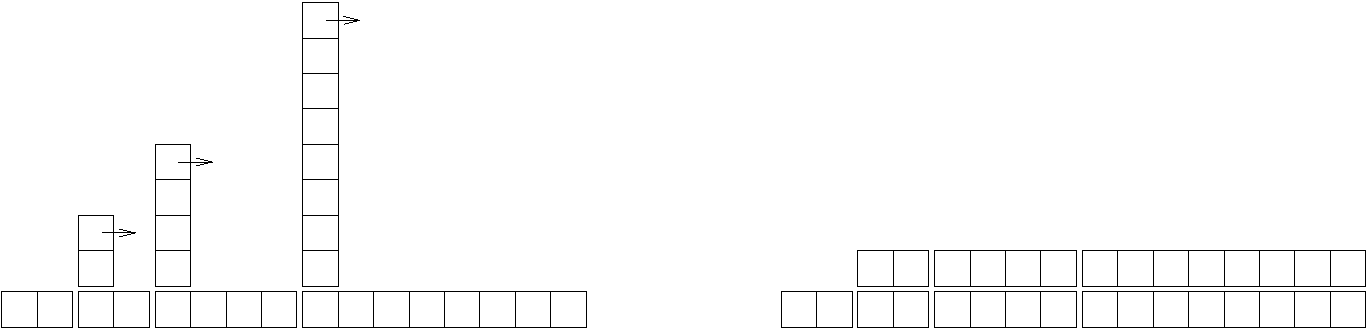
\includegraphics[width=5.5in]{figs/towers.pdf}}
\caption{ค่าใช้จ่ายของการเพิ่มแฮชเทเบิล\label{fig.hash}}
\end{figure}

% The extra work of rehashing appears as a sequence of increasingly
% tall towers with increasing space between them.  Now if you knock
% over the towers, spreading the cost of resizing over all
% adds, you can see graphically that the total cost after $n$
% adds is $2n - 2$.
งานพิเศษของการรีแฮชจะปรากฏเป็นลำดับของหอคอยที่สูงขึ้นเรื่อยๆ พร้อมช่องว่างระหว่างพวกเขาที่เพิ่มขึ้น 
ตอนนี้ถ้าคุณเคาะเหนือหอคอย กระจายค่าใช้จ่ายในการปรับขนาดไปยังการเพิ่มทั้งหมด 
คุณจะเห็นภาพกราฟิกว่าค่าใช้จ่ายทั้งหมดหลังจาก $n$ ครั้งเป็น $2n - 2$


% An important feature of this algorithm is that when we resize the
% HashTable it grows geometrically; that is, we multiply the size by a
% constant.  If you increase the size
% arithmetically---adding a fixed number each time---the average time
% per {\tt add} is linear.
คุณลักษณะที่สำคัญของอัลกอริธึมนี้คือเมื่อเราปรับขนาดตารางแฮชมันจะเติบโตในเชิงเรขาคณิต 
นั่นคือเราคูณขนาดด้วยค่าคงที่ หากคุณเพิ่มขนาดทางคณิตศาสตร์ คือการบวกจำนวนคงที่ในแต่ละครั้ง เวลาเฉลี่ยต่อการ{\tt เพิ่ม}จึงเป็นเส้นตรง
\index{geometric resizing}

% You can download my implementation of HashMap from
% \url{http://thinkpython2.com/code/Map.py}, but remember that there
% is no reason to use it; if you want a map, just use a Python dictionary.

คุณสามารถดาวน์โหลด HashMap ของฉันได้จาก \url{http://thinkpython2.com/code/Map.py} 
แต่จำไว้ว่าไม่มีเหตุผลที่จะใช้มัน หากคุณต้องการแผนที่ให้ใช้ดิกชันนารีของไพธอน

%\section{Glossary}
\section{อภิธานศัพท์}

\begin{description}

% \item[analysis of algorithms:] A way to compare algorithms in terms of
% their run time and/or space requirements.
\item[การวิเคราะห์อัลกอริทึม (analysis of algorithms):] วิธีเปรียบเทียบอัลกอริทึมในแง่ของเวลาใช้งานและ/หรือข้อกำหนดด้านพื้นที่
\index{analysis of algorithms}

% \item[machine model:] A simplified representation of a computer used
% to describe algorithms.
\item[โมเดลของเครื่อง (machine model):] การแทนอย่างง่ายสำหรับคอมพิวเตอร์เพื่อใช้อธิบายอัลกอริทึม
\index{machine model}

% \item[worst case:] The input that makes a given algorithm run slowest (or
% require the most space.
\item[กรณีที่แย่ที่สุด (worst case):] อินพุตที่ทำให้อัลกอริทึมที่สนใจทำงานช้าที่สุด (หรือต้องการพื้นที่มากที่สุด)
\index{worst case}

% \item[leading term:] In a polynomial, the term with the highest exponent.
\item[พจน์นำ (leading term):] พจน์ที่มีเลขชี้กำลังสูงสุดในพหุนาม
\index{leading term}

% \item[crossover point:] The problem size where two algorithms require
% the same run time or space. 
\item[จุดเปลี่ยน (crossover point):] ขนาดปัญหาที่อัลกอริธึมสองตัวต้องใช้เวลาหรือพื้นที่ทำงานเท่ากัน
\index{crossover point}

% \item[order of growth:] A set of functions that all grow in a way
% considered equivalent for purposes of analysis of algorithms. 
% For example, all functions that grow linearly belong to the same
% order of growth.
\item[ลำดับการเติบโต (order of growth):] ชุดของฟังก์ชันที่เติบโตในลักษณะที่เทียบเท่ากับวัตถุประสงค์ของการวิเคราะห์อัลกอริธึม 
ตัวอย่างเช่น ฟังก์ชันทั้งหมดที่เติบโตเชิงเส้นอยู่ในลำดับการเติบโตเดียวกัน
\index{order of growth}

% \item[Big-Oh notation:] Notation for representing an order of growth;
% for example, $O(n)$ represents the set of functions that grow
% linearly. 
\item[สัญกรณ์บิ๊กโอ (Big-Oh notation):] สัญกรณ์สำหรับแสดงลำดับการเติบโต ตัวอย่างเช่น $O(n)$ แทนชุดของฟังก์ชันที่เติบโตเป็นเส้นตรง
\index{Big-Oh notation}

% \item[linear:] An algorithm whose run time is proportional to
% problem size, at least for large problem sizes.
\item[เชิงเส้น (linear):] อัลกอริธึมที่เวลาทำงานเป็นสัดส่วนกับขนาดของปัญหา อย่างน้อยก็สำหรับปัญหาขนาดใหญ่
\index{linear}

% \item[quadratic:] An algorithm whose run time is proportional to
% $n^2$, where $n$ is a measure of problem size.
\item[กำลังสอง (quadratic):] อัลกอริทึมที่มีเวลาทำงานเป็นสัดส่วนกับ $n^2$ โดยที่ $n$ คือขนาดของปัญหา
\index{quadratic}

% \item[search:] The problem of locating an element of a collection
% (like a list or dictionary) or determining that it is not present.
\item[การค้นหา (search):] ปัญหาในการหาตำแหน่งองค์ประกอบของกลุ่มหมู่ (เช่น ลิสต์หรือดิกชันนารี) หรือการพิจารณาว่าไม่มีองค์ประกอบนั้น
\index{search}

% \item[hashtable:] A data structure that represents a collection of
% key-value pairs and performs search in constant time.
\item[ตารางแฮช (hashtable):] โครงสร้างข้อมูลที่แสดงถึงชุดของคู่คีย์-ค่าและทำการค้นหาในเวลาคงที่
\index{hashtable}

\end{description}

\printindex

\clearemptydoublepage
%\blankpage
%\blankpage
%\blankpage


\end{document}
